\section{Service--Communication Trade-off Sweep}

\label{sec:service-sweep}

This section reports the complete public-score sensitivity sweep supplied with the reproducibility package. Nine completed threshold/cap combinations are evaluated; every combination contains 120 runs per method (60 OPSD and 60 UCI), or 720 policy runs across the six methods and 6,480 policy runs over the full sweep. The coverage, recall, fidelity, fairness, traffic, and privacy-accounting definitions are unchanged. The threshold controls the public release score and $M$ bounds private releases per endpoint. These are operating controls rather than coverage guarantees.

\subsection{The sweep exposes a continuous service--traffic frontier}

Increasing the release cap moves PRISM-XAI toward higher-traffic, higher-service operating points. Across the observed settings, mean PRISM-XAI traffic increases from 205.41--208.83~kbit at $M=8$ to 342.50--345.42~kbit at $M=16$ and 574.63--584.33~kbit at $M=32$. Coverage rises from 0.044--0.078 to 0.086--0.131 and then 0.140--0.206. Critical-event recall follows the same broad pattern, rising from 0.021--0.037 to 0.040--0.059 and then 0.064--0.085. Thus, the low-traffic result is not a claim of uniformly superior monitoring service; the cap selects a point on the communication--service frontier.

\begin{table*}[htbp]

\caption{Observed PRISM-XAI operating points in the public-score service sweep. Savings are the ratio of aggregate mean traffic relative to MAP-XAI-only; paired confidence intervals are reported in Table~\ref{tab:sweep-paired}.}

\label{tab:sweep-means}

\centering\scriptsize

\begin{tabular}{rrrrrrrr}

\toprule

$\tau$ & $M$ & PRISM kbit & MAP kbit & Saving & Coverage & Recall & $\epsilon_{\max}$\\

\midrule

0.5 & 8 & 208.83 & 243.80 & 14.35\% & 0.0444 & 0.0209 & 18.206\\

1 & 8 & 206.42 & 243.80 & 15.33\% & 0.0510 & 0.0230 & 18.206\\

2 & 8 & 205.41 & 243.37 & 15.60\% & 0.0737 & 0.0367 & 18.206\\

3 & 8 & 207.31 & 243.71 & 14.94\% & 0.0779 & 0.0366 & 18.206\\

1 & 16 & 342.50 & 407.81 & 16.01\% & 0.0856 & 0.0401 & 17.727\\

2 & 16 & 343.07 & 407.50 & 15.81\% & 0.1248 & 0.0594 & 17.745\\

3 & 16 & 345.42 & 407.78 & 15.29\% & 0.1312 & 0.0594 & 17.777\\

1 & 32 & 574.63 & 688.64 & 16.56\% & 0.1402 & 0.0638 & 17.196\\

3 & 32 & 584.33 & 688.42 & 15.12\% & 0.2064 & 0.0852 & 17.301\\

\bottomrule

\end{tabular}

\end{table*}

\begin{table*}[htbp]

\caption{Paired PRISM-XAI minus MAP-XAI-only results for the nine sweep settings ($n=120$ pairs per row). Coverage and recall are proportions; CI is the 95\% half-width.}

\label{tab:sweep-paired}

\centering\scriptsize

\begin{tabular}{rrrrrrrr}

\toprule

$\tau$ & $M$ & $\Delta$ kbit & CI & $\Delta$ coverage & CI & $\Delta$ recall & CI\\

\midrule

0.5 & 8 & -34.97 & 3.06 & -0.00026 & 0.00046 & -0.00049 & 0.00107\\

1 & 8 & -37.38 & 3.49 & -0.00082 & 0.00060 & -0.00086 & 0.00107\\

2 & 8 & -37.96 & 3.63 & -0.00053 & 0.00046 & -0.00061 & 0.00143\\

3 & 8 & -36.40 & 3.32 & -0.00010 & 0.00043 & -0.00083 & 0.00156\\

1 & 16 & -65.31 & 7.13 & -0.00075 & 0.00093 & 0.00082 & 0.00162\\

2 & 16 & -64.43 & 7.17 & -0.00024 & 0.00023 & 0.00076 & 0.00208\\

3 & 16 & -62.36 & 6.82 & -0.00010 & 0.00034 & 0.00244 & 0.00227\\

1 & 32 & -114.01 & 15.13 & -0.00060 & 0.00111 & 0.00153 & 0.00178\\

3 & 32 & -104.09 & 13.56 & -0.00010 & 0.00026 & 0.00124 & 0.00307\\

\bottomrule

\end{tabular}

\end{table*}

The paired comparisons show traffic reductions at every tested setting, while the service changes are small in absolute terms. However, the declared descriptive-overlap rule is satisfied by MAP-XAI-only in all 12 dataset/explainer/privacy cells only for the four $M=8$ settings. It is satisfied in 8 of 12 cells at $M=16$, and in 4 of 12 cells for $(\tau,M)=(1,32)$ and 5 of 12 for $(3,32)$. The larger-cap points therefore describe the broader service frontier and are not additional matched-service confirmations of the headline claim.

\begin{figure*}[htbp]

\centering

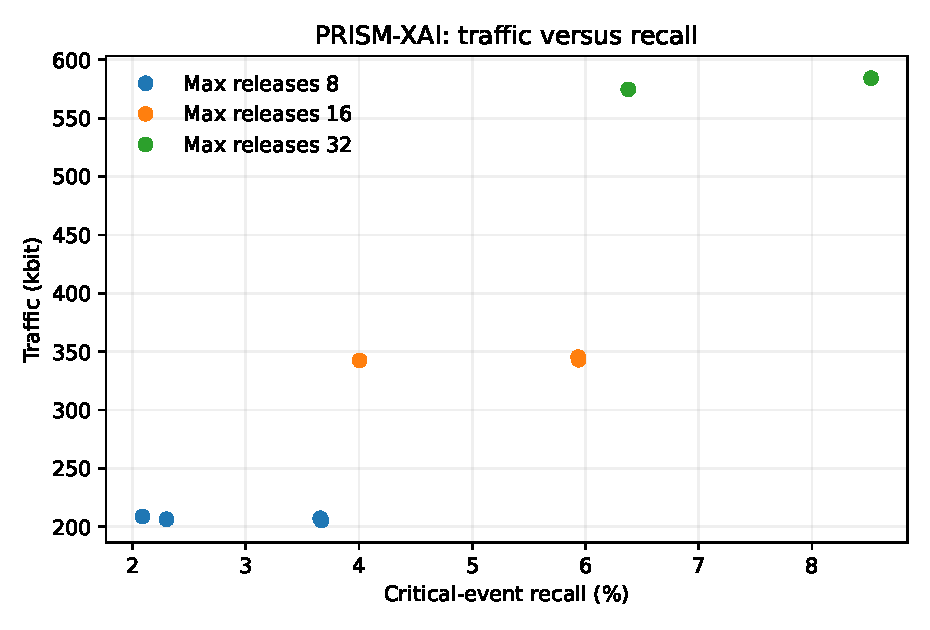
\includegraphics[width=.32\textwidth]{../../SERVICE_TRADEOFF_RESULTS/paper_evidence/traffic_vs_recall_prism.pdf}\hfill

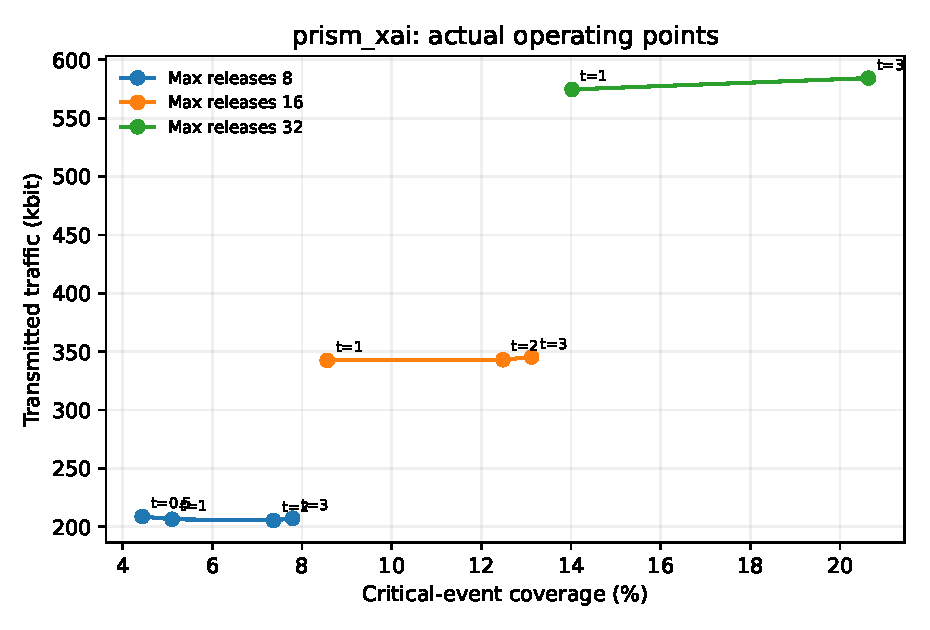
\includegraphics[width=.32\textwidth]{../../SERVICE_TRADEOFF_RESULTS/paper_evidence/traffic_vs_coverage_prism_xai.pdf}\hfill

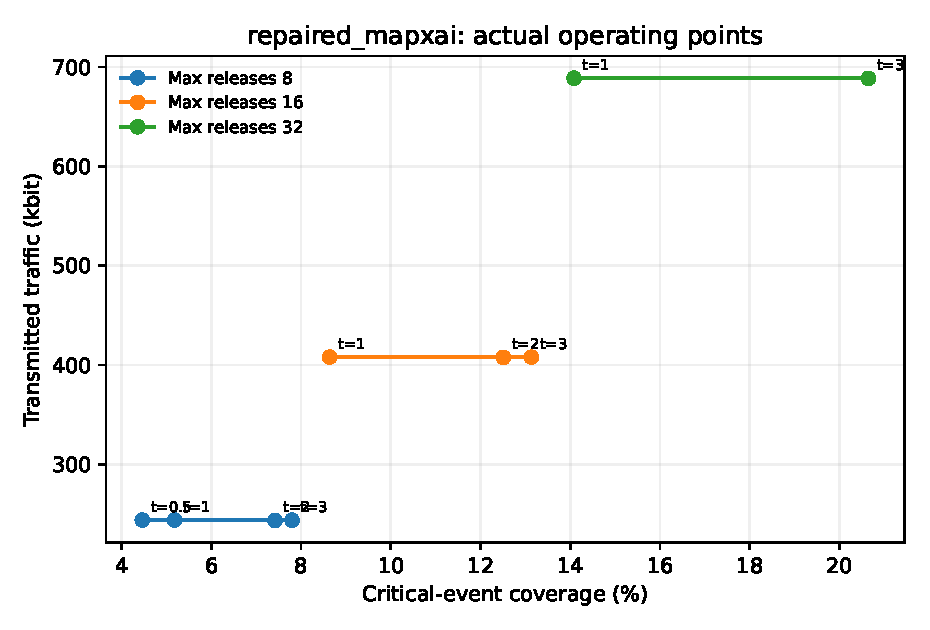
\includegraphics[width=.32\textwidth]{../../SERVICE_TRADEOFF_RESULTS/paper_evidence/traffic_vs_coverage_repaired_mapxai.pdf}

\caption{Service--communication frontier from all completed sweep settings. Left: PRISM-XAI traffic versus critical-event recall. Center: PRISM-XAI traffic versus intervention coverage. Right: MAP-XAI-only traffic versus coverage at the corresponding cap/threshold configurations. Moving to larger release caps increases both communication and the measured service proxies; the figures therefore support operating-point selection, not a traffic-only ranking.}

\label{fig:sweep-frontier}

\end{figure*}

\FloatBarrier

\subsection{Complete generated sweep evidence}

The following archive reproduces every generated vector figure and every generated LaTeX table for the nine settings at aggregate, OPSD, and UCI scope. Raster PNG counterparts, raw CSV files, JSON manifests, source hashes, and execution logs remain in the accompanying package. Each five-figure block is interpreted jointly: the trace shows temporal release behavior; fairness--reliability checks whether service is concentrated; privacy--fidelity relates recorded expenditure to attribution agreement; the Pareto plane displays communication cost against the fidelity proxy; and the ablation panel attributes changes to individual design elements. Tables preserve the complete method means, condition-level breakdowns, and paired contrasts.

\subsubsection{Public-score threshold $\tau=0.5$, release cap $M=8$}

At this operating point, PRISM-XAI transmits 208.83~kbit versus 243.80~kbit for MAP-XAI-only (aggregate-mean ratio saving 14.35\%). The paired difference is -34.97$\pm$3.06~kbit. PRISM coverage is 0.0444, critical-event recall is 0.0209, and maximum recorded expenditure is 18.206. Relative to MAP-XAI-only, the paired coverage change is -0.00026$\pm$0.00046 and recall change is -0.00049$\pm$0.00107. The descriptive overlap rule holds in 12 of 12 cells. Accordingly, this point is read as a matched-service scheduler comparison.

\paragraph{Combined datasets.} The three generated tables below report the full method means, all condition-level values, and paired differences. The five figures that follow provide the corresponding temporal, fairness, privacy, Pareto, and ablation views. Aggregate panels support the setting-level summary above; dataset panels reveal whether that summary is shared by OPSD and UCI rather than being driven by their different endpoint counts.

\begin{table*}[p]\centering\tiny

\caption{Public-score threshold $\tau=0.5$, release cap $M=8$, Combined datasets: complete generated method table.}

\label{tab:thr_0.5_cap_8:combined:main}

\resizebox{\linewidth}{!}{% Values are means with 95% Student-t confidence intervals across seeds.
\begin{tabular}{lccccccccccccccc}
\toprule
Dataset & Model & $\epsilon_{\max}$ & Method & Top-$K$ & Cosine & Decision & Recall & Prec. & Abst. & P95 ms & kbit & Spent $\epsilon$ & False int. & bit/correct & Fairness \\
\midrule
OPSD & Tree & 8 & AoX-aware fixed-DP & 0.234 $\pm$ 0.048 & -0.033 $\pm$ 0.028 & 0.119 $\pm$ 0.028 & 0.119 $\pm$ 0.028 & 0.198 $\pm$ 0.054 & 0.721 $\pm$ 0.005 & 6.903 $\pm$ 1.126 & 1560.564 $\pm$ 0.000 & 7.990 $\pm$ 0.000 & 0.183 $\pm$ 0.020 & 35567.482 $\pm$ 10569.818 & 0.999 $\pm$ 0.000 \\
OPSD & Tree & 8 & AoX-aware fixed-DP & 0.238 $\pm$ 0.049 & -0.026 $\pm$ 0.055 & 0.121 $\pm$ 0.026 & 0.121 $\pm$ 0.026 & 0.205 $\pm$ 0.053 & 0.721 $\pm$ 0.005 & 6.903 $\pm$ 1.126 & 1560.564 $\pm$ 0.000 & 7.990 $\pm$ 0.000 & 0.179 $\pm$ 0.023 & 34123.214 $\pm$ 8376.542 & 0.999 $\pm$ 0.000 \\
OPSD & Tree & 8 & Channel-aware fixed-DP & 0.292 $\pm$ 0.037 & -0.041 $\pm$ 0.051 & 0.107 $\pm$ 0.026 & 0.107 $\pm$ 0.026 & 0.217 $\pm$ 0.068 & 0.779 $\pm$ 0.011 & 5.571 $\pm$ 1.784 & 1560.564 $\pm$ 0.000 & 7.990 $\pm$ 0.000 & 0.154 $\pm$ 0.029 & 40860.756 $\pm$ 14126.920 & 0.999 $\pm$ 0.000 \\
OPSD & Tree & 8 & Channel-aware fixed-DP & 0.292 $\pm$ 0.054 & -0.049 $\pm$ 0.064 & 0.111 $\pm$ 0.023 & 0.111 $\pm$ 0.023 & 0.228 $\pm$ 0.066 & 0.779 $\pm$ 0.011 & 5.571 $\pm$ 1.784 & 1560.564 $\pm$ 0.000 & 7.990 $\pm$ 0.000 & 0.149 $\pm$ 0.026 & 37980.855 $\pm$ 12338.094 & 0.999 $\pm$ 0.000 \\
OPSD & Tree & 8 & Joint, no compression & 0.288 $\pm$ 0.064 & -0.030 $\pm$ 0.079 & 0.016 $\pm$ 0.005 & 0.016 $\pm$ 0.005 & 0.193 $\pm$ 0.059 & 0.957 $\pm$ 0.003 & 4.560 $\pm$ 1.811 & 189.900 $\pm$ 0.554 & 7.990 $\pm$ 0.000 & 0.027 $\pm$ 0.005 & 32490.357 $\pm$ 10149.755 & 0.996 $\pm$ 0.002 \\
OPSD & Tree & 8 & Joint, no compression & 0.258 $\pm$ 0.055 & 0.011 $\pm$ 0.094 & 0.019 $\pm$ 0.004 & 0.019 $\pm$ 0.004 & 0.224 $\pm$ 0.044 & 0.957 $\pm$ 0.003 & 4.562 $\pm$ 1.809 & 189.750 $\pm$ 0.566 & 7.990 $\pm$ 0.000 & 0.025 $\pm$ 0.003 & 26079.167 $\pm$ 6335.386 & 0.996 $\pm$ 0.002 \\
OPSD & Tree & 8 & Periodic fixed-DP & 0.241 $\pm$ 0.049 & -0.019 $\pm$ 0.061 & 0.125 $\pm$ 0.020 & 0.125 $\pm$ 0.020 & 0.209 $\pm$ 0.044 & 0.722 $\pm$ 0.006 & 6.303 $\pm$ 1.438 & 1560.564 $\pm$ 0.000 & 7.990 $\pm$ 0.000 & 0.181 $\pm$ 0.021 & 31183.082 $\pm$ 4356.378 & 0.999 $\pm$ 0.000 \\
OPSD & Tree & 8 & Periodic fixed-DP & 0.242 $\pm$ 0.048 & -0.026 $\pm$ 0.082 & 0.135 $\pm$ 0.016 & 0.135 $\pm$ 0.016 & 0.231 $\pm$ 0.037 & 0.722 $\pm$ 0.006 & 6.303 $\pm$ 1.438 & 1560.564 $\pm$ 0.000 & 7.990 $\pm$ 0.000 & 0.169 $\pm$ 0.017 & 28520.235 $\pm$ 3511.595 & 0.999 $\pm$ 0.000 \\
OPSD & Tree & 8 & PRISM-XAI & 0.227 $\pm$ 0.040 & -0.036 $\pm$ 0.078 & 0.013 $\pm$ 0.005 & 0.013 $\pm$ 0.005 & 0.218 $\pm$ 0.087 & 0.964 $\pm$ 0.002 & 4.341 $\pm$ 1.447 & 87.697 $\pm$ 0.388 & 7.823 $\pm$ 0.000 & 0.018 $\pm$ 0.005 & 24929.927 $\pm$ 17099.604 & 0.993 $\pm$ 0.004 \\
OPSD & Tree & 8 & PRISM-XAI & 0.198 $\pm$ 0.035 & -0.021 $\pm$ 0.089 & 0.013 $\pm$ 0.005 & 0.013 $\pm$ 0.005 & 0.210 $\pm$ 0.097 & 0.964 $\pm$ 0.002 & 4.332 $\pm$ 1.445 & 87.461 $\pm$ 0.318 & 7.823 $\pm$ 0.000 & 0.019 $\pm$ 0.005 & 25702.427 $\pm$ 16465.572 & 0.993 $\pm$ 0.004 \\
OPSD & Tree & 8 & MAP-XAI fallback & 0.254 $\pm$ 0.049 & -0.070 $\pm$ 0.094 & 0.015 $\pm$ 0.005 & 0.015 $\pm$ 0.005 & 0.263 $\pm$ 0.086 & 0.964 $\pm$ 0.002 & 4.453 $\pm$ 1.383 & 105.817 $\pm$ 0.049 & 7.823 $\pm$ 0.000 & 0.016 $\pm$ 0.004 & 21748.429 $\pm$ 9602.332 & 0.993 $\pm$ 0.004 \\
OPSD & Tree & 8 & MAP-XAI fallback & 0.237 $\pm$ 0.043 & -0.048 $\pm$ 0.094 & 0.013 $\pm$ 0.006 & 0.013 $\pm$ 0.006 & 0.226 $\pm$ 0.081 & 0.964 $\pm$ 0.002 & 4.453 $\pm$ 1.383 & 105.675 $\pm$ 0.049 & 7.823 $\pm$ 0.000 & 0.017 $\pm$ 0.003 & 26069.368 $\pm$ 11426.445 & 0.993 $\pm$ 0.004 \\
UCI & Tree & 8 & AoX-aware fixed-DP & 0.263 $\pm$ 0.041 & -0.007 $\pm$ 0.009 & 0.457 $\pm$ 0.031 & 0.457 $\pm$ 0.031 & 0.362 $\pm$ 0.024 & 0.003 $\pm$ 0.001 & 7.500 $\pm$ 0.000 & 5300.224 $\pm$ 0.000 & 7.990 $\pm$ 0.000 & 0.557 $\pm$ 0.025 & 14002.896 $\pm$ 1040.243 & 0.999 $\pm$ 0.000 \\
UCI & Tree & 8 & AoX-aware fixed-DP & 0.260 $\pm$ 0.022 & 0.010 $\pm$ 0.055 & 0.455 $\pm$ 0.047 & 0.455 $\pm$ 0.047 & 0.361 $\pm$ 0.038 & 0.003 $\pm$ 0.001 & 7.500 $\pm$ 0.000 & 5300.224 $\pm$ 0.000 & 7.990 $\pm$ 0.000 & 0.557 $\pm$ 0.048 & 14198.303 $\pm$ 1508.274 & 0.999 $\pm$ 0.000 \\
UCI & Tree & 8 & Channel-aware fixed-DP & 0.248 $\pm$ 0.031 & 0.004 $\pm$ 0.012 & 0.001 $\pm$ 0.001 & 0.001 $\pm$ 0.001 & 0.150 $\pm$ 0.151 & 0.999 $\pm$ 0.001 & 4.609 $\pm$ 1.781 & 5295.177 $\pm$ 3.740 & 7.990 $\pm$ 0.000 & 0.001 $\pm$ 0.001 & 4632196.500 $\pm$ 2102650.252 & 0.991 $\pm$ 0.001 \\
UCI & Tree & 8 & Channel-aware fixed-DP & 0.239 $\pm$ 0.030 & -0.020 $\pm$ 0.055 & 0.000 $\pm$ 0.000 & 0.000 $\pm$ 0.000 & 0.117 $\pm$ 0.225 & 0.999 $\pm$ 0.001 & 4.609 $\pm$ 1.781 & 5295.177 $\pm$ 3.740 & 7.990 $\pm$ 0.000 & 0.001 $\pm$ 0.001 & 5296989.000 $\pm$ 41104.572 & 0.991 $\pm$ 0.001 \\
UCI & Tree & 8 & Joint, no compression & 0.286 $\pm$ 0.045 & 0.004 $\pm$ 0.020 & 0.052 $\pm$ 0.005 & 0.052 $\pm$ 0.005 & 0.406 $\pm$ 0.037 & 0.875 $\pm$ 0.003 & 5.123 $\pm$ 1.792 & 672.300 $\pm$ 0.452 & 7.990 $\pm$ 0.000 & 0.053 $\pm$ 0.004 & 15676.175 $\pm$ 1475.621 & 0.994 $\pm$ 0.003 \\
UCI & Tree & 8 & Joint, no compression & 0.229 $\pm$ 0.052 & -0.032 $\pm$ 0.050 & 0.057 $\pm$ 0.007 & 0.057 $\pm$ 0.007 & 0.428 $\pm$ 0.041 & 0.875 $\pm$ 0.003 & 5.131 $\pm$ 1.787 & 672.300 $\pm$ 0.452 & 7.990 $\pm$ 0.000 & 0.052 $\pm$ 0.004 & 14702.786 $\pm$ 2334.488 & 0.994 $\pm$ 0.003 \\
UCI & Tree & 8 & Periodic fixed-DP & 0.259 $\pm$ 0.060 & -0.005 $\pm$ 0.008 & 0.006 $\pm$ 0.001 & 0.006 $\pm$ 0.001 & 0.244 $\pm$ 0.049 & 0.989 $\pm$ 0.001 & 4.596 $\pm$ 1.788 & 5299.318 $\pm$ 1.451 & 7.786 $\pm$ 0.000 & 0.013 $\pm$ 0.002 & 1215103.896 $\pm$ 390671.319 & 0.999 $\pm$ 0.000 \\
UCI & Tree & 8 & Periodic fixed-DP & 0.260 $\pm$ 0.044 & 0.022 $\pm$ 0.070 & 0.005 $\pm$ 0.001 & 0.005 $\pm$ 0.001 & 0.195 $\pm$ 0.050 & 0.989 $\pm$ 0.001 & 4.596 $\pm$ 1.788 & 5299.318 $\pm$ 1.451 & 7.786 $\pm$ 0.000 & 0.015 $\pm$ 0.002 & 1555837.203 $\pm$ 955472.503 & 0.999 $\pm$ 0.000 \\
UCI & Tree & 8 & PRISM-XAI & 0.238 $\pm$ 0.091 & 0.008 $\pm$ 0.022 & 0.028 $\pm$ 0.004 & 0.028 $\pm$ 0.004 & 0.465 $\pm$ 0.035 & 0.940 $\pm$ 0.003 & 4.723 $\pm$ 1.732 & 330.248 $\pm$ 1.899 & 7.823 $\pm$ 0.000 & 0.022 $\pm$ 0.002 & 14725.609 $\pm$ 2267.563 & 0.991 $\pm$ 0.003 \\
UCI & Tree & 8 & PRISM-XAI & 0.233 $\pm$ 0.050 & -0.032 $\pm$ 0.070 & 0.026 $\pm$ 0.003 & 0.026 $\pm$ 0.003 & 0.454 $\pm$ 0.085 & 0.945 $\pm$ 0.005 & 4.249 $\pm$ 1.633 & 327.398 $\pm$ 2.091 & 7.823 $\pm$ 0.000 & 0.022 $\pm$ 0.005 & 15910.590 $\pm$ 2766.316 & 0.991 $\pm$ 0.004 \\
UCI & Tree & 8 & MAP-XAI fallback & 0.224 $\pm$ 0.053 & 0.017 $\pm$ 0.017 & 0.027 $\pm$ 0.005 & 0.027 $\pm$ 0.005 & 0.459 $\pm$ 0.057 & 0.940 $\pm$ 0.003 & 4.895 $\pm$ 1.639 & 382.160 $\pm$ 0.072 & 7.823 $\pm$ 0.000 & 0.021 $\pm$ 0.002 & 17976.663 $\pm$ 3232.835 & 0.990 $\pm$ 0.003 \\
UCI & Tree & 8 & MAP-XAI fallback & 0.251 $\pm$ 0.037 & -0.011 $\pm$ 0.080 & 0.026 $\pm$ 0.006 & 0.026 $\pm$ 0.006 & 0.462 $\pm$ 0.081 & 0.943 $\pm$ 0.006 & 5.591 $\pm$ 1.764 & 381.645 $\pm$ 0.090 & 7.823 $\pm$ 0.000 & 0.021 $\pm$ 0.005 & 18792.055 $\pm$ 3629.218 & 0.989 $\pm$ 0.004 \\
\bottomrule
\end{tabular}
}

\end{table*}\clearpage

\begin{table*}[p]\centering\tiny

\caption{Public-score threshold $\tau=0.5$, release cap $M=8$, Combined datasets: complete condition-level generated table.}

\label{tab:thr_0.5_cap_8:combined:conditions}

\resizebox{\textwidth}{!}{\begin{tabular}{llllccccccccccc}
\toprule
Dataset & Model & $\epsilon_{\max}$ & Method & kbit & Top-$K$ & Random Top-$K$ & Cosine & Decision & Recall & Precision & Coverage & Abstain & False int. & Spent $\epsilon$ \\
\midrule
OPSD & Tree & 8 & Joint, no compression & 189.900 $\pm$ 0.554 & 0.288 $\pm$ 0.064 & 0.250 $\pm$ 0.000 & -0.030 $\pm$ 0.079 & 0.016 $\pm$ 0.005 & 0.016 $\pm$ 0.005 & 0.193 $\pm$ 0.059 & 0.043 $\pm$ 0.003 & 0.957 $\pm$ 0.003 & 0.027 $\pm$ 0.005 & 7.990 $\pm$ 0.000 \\
OPSD & Tree & 8 & Joint, no compression & 189.750 $\pm$ 0.566 & 0.258 $\pm$ 0.055 & 0.250 $\pm$ 0.000 & 0.011 $\pm$ 0.094 & 0.019 $\pm$ 0.004 & 0.019 $\pm$ 0.004 & 0.224 $\pm$ 0.044 & 0.043 $\pm$ 0.003 & 0.957 $\pm$ 0.003 & 0.025 $\pm$ 0.003 & 7.990 $\pm$ 0.000 \\
OPSD & Tree & 8 & Periodic fixed-DP & 1560.564 $\pm$ 0.000 & 0.241 $\pm$ 0.049 & 0.250 $\pm$ 0.000 & -0.019 $\pm$ 0.061 & 0.125 $\pm$ 0.020 & 0.125 $\pm$ 0.020 & 0.209 $\pm$ 0.044 & 0.278 $\pm$ 0.006 & 0.722 $\pm$ 0.006 & 0.181 $\pm$ 0.021 & 7.990 $\pm$ 0.000 \\
OPSD & Tree & 8 & Periodic fixed-DP & 1560.564 $\pm$ 0.000 & 0.242 $\pm$ 0.048 & 0.250 $\pm$ 0.000 & -0.026 $\pm$ 0.082 & 0.135 $\pm$ 0.016 & 0.135 $\pm$ 0.016 & 0.231 $\pm$ 0.037 & 0.278 $\pm$ 0.006 & 0.722 $\pm$ 0.006 & 0.169 $\pm$ 0.017 & 7.990 $\pm$ 0.000 \\
OPSD & Tree & 8 & PRISM-XAI & 87.697 $\pm$ 0.388 & 0.227 $\pm$ 0.040 & 0.250 $\pm$ 0.000 & -0.036 $\pm$ 0.078 & 0.013 $\pm$ 0.005 & 0.013 $\pm$ 0.005 & 0.218 $\pm$ 0.087 & 0.036 $\pm$ 0.002 & 0.964 $\pm$ 0.002 & 0.018 $\pm$ 0.005 & 7.823 $\pm$ 0.000 \\
OPSD & Tree & 8 & PRISM-XAI & 87.461 $\pm$ 0.318 & 0.198 $\pm$ 0.035 & 0.250 $\pm$ 0.000 & -0.021 $\pm$ 0.089 & 0.013 $\pm$ 0.005 & 0.013 $\pm$ 0.005 & 0.210 $\pm$ 0.097 & 0.036 $\pm$ 0.002 & 0.964 $\pm$ 0.002 & 0.019 $\pm$ 0.005 & 7.823 $\pm$ 0.000 \\
OPSD & Tree & 16 & Joint, no compression & 459.900 $\pm$ 0.750 & 0.232 $\pm$ 0.065 & 0.250 $\pm$ 0.000 & 0.059 $\pm$ 0.048 & 0.038 $\pm$ 0.009 & 0.038 $\pm$ 0.009 & 0.222 $\pm$ 0.049 & 0.088 $\pm$ 0.004 & 0.912 $\pm$ 0.004 & 0.049 $\pm$ 0.005 & 15.997 $\pm$ 0.000 \\
OPSD & Tree & 16 & Joint, no compression & 460.050 $\pm$ 0.724 & 0.241 $\pm$ 0.055 & 0.250 $\pm$ 0.000 & 0.061 $\pm$ 0.052 & 0.039 $\pm$ 0.008 & 0.039 $\pm$ 0.008 & 0.241 $\pm$ 0.042 & 0.088 $\pm$ 0.004 & 0.912 $\pm$ 0.004 & 0.045 $\pm$ 0.004 & 15.997 $\pm$ 0.000 \\
OPSD & Tree & 16 & Periodic fixed-DP & 5112.594 $\pm$ 0.000 & 0.249 $\pm$ 0.022 & 0.250 $\pm$ 0.000 & -0.009 $\pm$ 0.045 & 0.450 $\pm$ 0.062 & 0.450 $\pm$ 0.062 & 0.237 $\pm$ 0.042 & 0.985 $\pm$ 0.002 & 0.015 $\pm$ 0.002 & 0.551 $\pm$ 0.057 & 15.997 $\pm$ 0.000 \\
OPSD & Tree & 16 & Periodic fixed-DP & 5112.594 $\pm$ 0.000 & 0.243 $\pm$ 0.019 & 0.250 $\pm$ 0.000 & -0.012 $\pm$ 0.050 & 0.463 $\pm$ 0.047 & 0.463 $\pm$ 0.047 & 0.240 $\pm$ 0.028 & 0.985 $\pm$ 0.002 & 0.015 $\pm$ 0.002 & 0.547 $\pm$ 0.036 & 15.997 $\pm$ 0.000 \\
OPSD & Tree & 16 & PRISM-XAI & 87.635 $\pm$ 0.376 & 0.225 $\pm$ 0.047 & 0.250 $\pm$ 0.000 & 0.065 $\pm$ 0.050 & 0.016 $\pm$ 0.004 & 0.016 $\pm$ 0.004 & 0.293 $\pm$ 0.081 & 0.036 $\pm$ 0.002 & 0.964 $\pm$ 0.002 & 0.015 $\pm$ 0.004 & 15.620 $\pm$ 0.000 \\
OPSD & Tree & 16 & PRISM-XAI & 87.431 $\pm$ 0.305 & 0.188 $\pm$ 0.051 & 0.250 $\pm$ 0.000 & 0.103 $\pm$ 0.067 & 0.017 $\pm$ 0.005 & 0.017 $\pm$ 0.005 & 0.302 $\pm$ 0.076 & 0.036 $\pm$ 0.002 & 0.964 $\pm$ 0.002 & 0.015 $\pm$ 0.004 & 15.620 $\pm$ 0.000 \\
OPSD & Tree & 32 & Joint, no compression & 1140.900 $\pm$ 7.953 & 0.235 $\pm$ 0.064 & 0.250 $\pm$ 0.000 & -0.031 $\pm$ 0.089 & 0.074 $\pm$ 0.015 & 0.074 $\pm$ 0.015 & 0.205 $\pm$ 0.039 & 0.157 $\pm$ 0.006 & 0.843 $\pm$ 0.006 & 0.107 $\pm$ 0.009 & 31.999 $\pm$ 0.000 \\
OPSD & Tree & 32 & Joint, no compression & 1140.900 $\pm$ 7.953 & 0.282 $\pm$ 0.054 & 0.250 $\pm$ 0.000 & -0.044 $\pm$ 0.076 & 0.080 $\pm$ 0.011 & 0.080 $\pm$ 0.011 & 0.227 $\pm$ 0.052 & 0.158 $\pm$ 0.006 & 0.842 $\pm$ 0.006 & 0.105 $\pm$ 0.015 & 31.999 $\pm$ 0.000 \\
OPSD & Tree & 32 & Periodic fixed-DP & 5299.836 $\pm$ 0.625 & 0.249 $\pm$ 0.022 & 0.250 $\pm$ 0.000 & -0.009 $\pm$ 0.044 & 0.458 $\pm$ 0.066 & 0.458 $\pm$ 0.066 & 0.237 $\pm$ 0.045 & 1.000 $\pm$ 0.000 & 0.000 $\pm$ 0.000 & 0.562 $\pm$ 0.062 & 16.371 $\pm$ 0.000 \\
OPSD & Tree & 32 & Periodic fixed-DP & 5299.836 $\pm$ 0.625 & 0.244 $\pm$ 0.019 & 0.250 $\pm$ 0.000 & -0.012 $\pm$ 0.050 & 0.471 $\pm$ 0.049 & 0.471 $\pm$ 0.049 & 0.240 $\pm$ 0.029 & 1.000 $\pm$ 0.000 & 0.000 $\pm$ 0.000 & 0.559 $\pm$ 0.039 & 16.371 $\pm$ 0.000 \\
OPSD & Tree & 32 & PRISM-XAI & 87.574 $\pm$ 0.349 & 0.335 $\pm$ 0.044 & 0.250 $\pm$ 0.000 & 0.205 $\pm$ 0.062 & 0.020 $\pm$ 0.003 & 0.020 $\pm$ 0.003 & 0.478 $\pm$ 0.125 & 0.036 $\pm$ 0.002 & 0.964 $\pm$ 0.002 & 0.010 $\pm$ 0.004 & 31.175 $\pm$ 0.000 \\
OPSD & Tree & 32 & PRISM-XAI & 87.216 $\pm$ 0.281 & 0.311 $\pm$ 0.061 & 0.250 $\pm$ 0.000 & 0.292 $\pm$ 0.078 & 0.022 $\pm$ 0.004 & 0.022 $\pm$ 0.004 & 0.495 $\pm$ 0.133 & 0.036 $\pm$ 0.002 & 0.964 $\pm$ 0.002 & 0.009 $\pm$ 0.004 & 31.175 $\pm$ 0.000 \\
UCI & Tree & 8 & Joint, no compression & 672.300 $\pm$ 0.452 & 0.286 $\pm$ 0.045 & 0.250 $\pm$ 0.000 & 0.004 $\pm$ 0.020 & 0.052 $\pm$ 0.005 & 0.052 $\pm$ 0.005 & 0.406 $\pm$ 0.037 & 0.125 $\pm$ 0.003 & 0.875 $\pm$ 0.003 & 0.053 $\pm$ 0.004 & 7.990 $\pm$ 0.000 \\
UCI & Tree & 8 & Joint, no compression & 672.300 $\pm$ 0.452 & 0.229 $\pm$ 0.052 & 0.250 $\pm$ 0.000 & -0.032 $\pm$ 0.050 & 0.057 $\pm$ 0.007 & 0.057 $\pm$ 0.007 & 0.428 $\pm$ 0.041 & 0.125 $\pm$ 0.003 & 0.875 $\pm$ 0.003 & 0.052 $\pm$ 0.004 & 7.990 $\pm$ 0.000 \\
UCI & Tree & 8 & Periodic fixed-DP & 5299.318 $\pm$ 1.451 & 0.259 $\pm$ 0.060 & 0.250 $\pm$ 0.000 & -0.005 $\pm$ 0.008 & 0.006 $\pm$ 0.001 & 0.006 $\pm$ 0.001 & 0.244 $\pm$ 0.049 & 0.011 $\pm$ 0.001 & 0.989 $\pm$ 0.001 & 0.013 $\pm$ 0.002 & 7.786 $\pm$ 0.000 \\
UCI & Tree & 8 & Periodic fixed-DP & 5299.318 $\pm$ 1.451 & 0.260 $\pm$ 0.044 & 0.250 $\pm$ 0.000 & 0.022 $\pm$ 0.070 & 0.005 $\pm$ 0.001 & 0.005 $\pm$ 0.001 & 0.195 $\pm$ 0.050 & 0.011 $\pm$ 0.001 & 0.989 $\pm$ 0.001 & 0.015 $\pm$ 0.002 & 7.786 $\pm$ 0.000 \\
UCI & Tree & 8 & PRISM-XAI & 330.248 $\pm$ 1.899 & 0.238 $\pm$ 0.091 & 0.250 $\pm$ 0.000 & 0.008 $\pm$ 0.022 & 0.028 $\pm$ 0.004 & 0.028 $\pm$ 0.004 & 0.465 $\pm$ 0.035 & 0.060 $\pm$ 0.003 & 0.940 $\pm$ 0.003 & 0.022 $\pm$ 0.002 & 7.823 $\pm$ 0.000 \\
UCI & Tree & 8 & PRISM-XAI & 327.398 $\pm$ 2.091 & 0.233 $\pm$ 0.050 & 0.250 $\pm$ 0.000 & -0.032 $\pm$ 0.070 & 0.026 $\pm$ 0.003 & 0.026 $\pm$ 0.003 & 0.454 $\pm$ 0.085 & 0.055 $\pm$ 0.005 & 0.945 $\pm$ 0.005 & 0.022 $\pm$ 0.005 & 7.823 $\pm$ 0.000 \\
UCI & Tree & 16 & Joint, no compression & 1632.150 $\pm$ 0.339 & 0.216 $\pm$ 0.041 & 0.250 $\pm$ 0.000 & 0.001 $\pm$ 0.012 & 0.094 $\pm$ 0.005 & 0.094 $\pm$ 0.005 & 0.330 $\pm$ 0.024 & 0.228 $\pm$ 0.005 & 0.772 $\pm$ 0.005 & 0.133 $\pm$ 0.010 & 15.997 $\pm$ 0.000 \\
UCI & Tree & 16 & Joint, no compression & 1632.600 $\pm$ 0.554 & 0.204 $\pm$ 0.011 & 0.250 $\pm$ 0.000 & -0.021 $\pm$ 0.033 & 0.099 $\pm$ 0.016 & 0.099 $\pm$ 0.016 & 0.347 $\pm$ 0.054 & 0.228 $\pm$ 0.005 & 0.772 $\pm$ 0.005 & 0.128 $\pm$ 0.011 & 15.997 $\pm$ 0.000 \\
UCI & Tree & 16 & Periodic fixed-DP & 5299.318 $\pm$ 1.451 & 0.259 $\pm$ 0.060 & 0.250 $\pm$ 0.000 & -0.005 $\pm$ 0.008 & 0.006 $\pm$ 0.001 & 0.006 $\pm$ 0.001 & 0.244 $\pm$ 0.049 & 0.011 $\pm$ 0.001 & 0.989 $\pm$ 0.001 & 0.013 $\pm$ 0.002 & 7.786 $\pm$ 0.000 \\
UCI & Tree & 16 & Periodic fixed-DP & 5299.318 $\pm$ 1.451 & 0.260 $\pm$ 0.044 & 0.250 $\pm$ 0.000 & 0.022 $\pm$ 0.070 & 0.005 $\pm$ 0.001 & 0.005 $\pm$ 0.001 & 0.195 $\pm$ 0.050 & 0.011 $\pm$ 0.001 & 0.989 $\pm$ 0.001 & 0.015 $\pm$ 0.002 & 7.786 $\pm$ 0.000 \\
UCI & Tree & 16 & PRISM-XAI & 330.309 $\pm$ 1.645 & 0.201 $\pm$ 0.066 & 0.250 $\pm$ 0.000 & 0.022 $\pm$ 0.015 & 0.027 $\pm$ 0.005 & 0.027 $\pm$ 0.005 & 0.573 $\pm$ 0.085 & 0.058 $\pm$ 0.004 & 0.942 $\pm$ 0.004 & 0.015 $\pm$ 0.004 & 15.620 $\pm$ 0.000 \\
UCI & Tree & 16 & PRISM-XAI & 329.517 $\pm$ 1.193 & 0.267 $\pm$ 0.020 & 0.250 $\pm$ 0.000 & 0.044 $\pm$ 0.071 & 0.022 $\pm$ 0.003 & 0.022 $\pm$ 0.003 & 0.521 $\pm$ 0.092 & 0.048 $\pm$ 0.004 & 0.952 $\pm$ 0.004 & 0.015 $\pm$ 0.005 & 15.620 $\pm$ 0.000 \\
UCI & Tree & 32 & Joint, no compression & 4034.550 $\pm$ 5.034 & 0.246 $\pm$ 0.031 & 0.250 $\pm$ 0.000 & -0.002 $\pm$ 0.015 & 0.228 $\pm$ 0.013 & 0.228 $\pm$ 0.013 & 0.361 $\pm$ 0.028 & 0.537 $\pm$ 0.009 & 0.463 $\pm$ 0.009 & 0.279 $\pm$ 0.017 & 31.999 $\pm$ 0.000 \\
UCI & Tree & 32 & Joint, no compression & 4034.550 $\pm$ 5.034 & 0.241 $\pm$ 0.033 & 0.250 $\pm$ 0.000 & -0.012 $\pm$ 0.030 & 0.228 $\pm$ 0.028 & 0.228 $\pm$ 0.028 & 0.360 $\pm$ 0.047 & 0.530 $\pm$ 0.010 & 0.470 $\pm$ 0.010 & 0.280 $\pm$ 0.026 & 31.999 $\pm$ 0.000 \\
UCI & Tree & 32 & Periodic fixed-DP & 5299.318 $\pm$ 1.451 & 0.259 $\pm$ 0.060 & 0.250 $\pm$ 0.000 & -0.005 $\pm$ 0.008 & 0.006 $\pm$ 0.001 & 0.006 $\pm$ 0.001 & 0.244 $\pm$ 0.049 & 0.011 $\pm$ 0.001 & 0.989 $\pm$ 0.001 & 0.013 $\pm$ 0.002 & 7.786 $\pm$ 0.000 \\
UCI & Tree & 32 & Periodic fixed-DP & 5299.318 $\pm$ 1.451 & 0.260 $\pm$ 0.044 & 0.250 $\pm$ 0.000 & 0.022 $\pm$ 0.070 & 0.005 $\pm$ 0.001 & 0.005 $\pm$ 0.001 & 0.195 $\pm$ 0.050 & 0.011 $\pm$ 0.001 & 0.989 $\pm$ 0.001 & 0.015 $\pm$ 0.002 & 7.786 $\pm$ 0.000 \\
UCI & Tree & 32 & PRISM-XAI & 332.151 $\pm$ 1.868 & 0.356 $\pm$ 0.056 & 0.250 $\pm$ 0.000 & 0.033 $\pm$ 0.016 & 0.023 $\pm$ 0.005 & 0.023 $\pm$ 0.005 & 0.969 $\pm$ 0.031 & 0.053 $\pm$ 0.005 & 0.947 $\pm$ 0.005 & 0.000 $\pm$ 0.001 & 31.175 $\pm$ 0.000 \\
UCI & Tree & 32 & PRISM-XAI & 331.266 $\pm$ 1.432 & 0.321 $\pm$ 0.046 & 0.250 $\pm$ 0.000 & 0.200 $\pm$ 0.047 & 0.024 $\pm$ 0.004 & 0.024 $\pm$ 0.004 & 0.943 $\pm$ 0.048 & 0.046 $\pm$ 0.003 & 0.954 $\pm$ 0.003 & 0.001 $\pm$ 0.001 & 31.175 $\pm$ 0.000 \\
\bottomrule
\end{tabular}
}

\end{table*}\clearpage

\begin{table*}[p]\centering\tiny

\caption{Public-score threshold $\tau=0.5$, release cap $M=8$, Combined datasets: complete generated paired comparisons.}

\label{tab:thr_0.5_cap_8:combined:paired}

\resizebox{\textwidth}{!}{\begin{tabular}{llcccc}
\toprule
Dataset & Baseline & Delta kbit & Delta Top-$K$ & Delta recall & Delta fairness \\
\midrule
OPSD & AoX-aware fixed-DP & -1472.867 $\pm$ 0.388 & -0.007 $\pm$ 0.067 & -0.106 $\pm$ 0.030 & -0.007 $\pm$ 0.003 \\
OPSD & AoX-aware fixed-DP & -5012.277 $\pm$ 5.554 & -0.029 $\pm$ 0.038 & -0.385 $\pm$ 0.074 & -0.007 $\pm$ 0.004 \\
OPSD & AoX-aware fixed-DP & -5212.650 $\pm$ 0.349 & 0.082 $\pm$ 0.065 & -0.392 $\pm$ 0.079 & -0.007 $\pm$ 0.004 \\
OPSD & AoX-aware fixed-DP & -1473.103 $\pm$ 0.318 & -0.040 $\pm$ 0.037 & -0.108 $\pm$ 0.027 & -0.007 $\pm$ 0.003 \\
OPSD & AoX-aware fixed-DP & -5012.482 $\pm$ 5.458 & -0.064 $\pm$ 0.038 & -0.397 $\pm$ 0.056 & -0.007 $\pm$ 0.004 \\
OPSD & AoX-aware fixed-DP & -5213.008 $\pm$ 0.281 & 0.060 $\pm$ 0.073 & -0.403 $\pm$ 0.058 & -0.006 $\pm$ 0.004 \\
OPSD & Channel-aware fixed-DP & -1472.867 $\pm$ 0.388 & -0.066 $\pm$ 0.052 & -0.094 $\pm$ 0.027 & -0.007 $\pm$ 0.003 \\
OPSD & Channel-aware fixed-DP & -4598.974 $\pm$ 13.023 & -0.037 $\pm$ 0.042 & -0.385 $\pm$ 0.089 & 0.055 $\pm$ 0.005 \\
OPSD & Channel-aware fixed-DP & -5212.650 $\pm$ 0.349 & 0.077 $\pm$ 0.057 & -0.414 $\pm$ 0.099 & 0.086 $\pm$ 0.006 \\
OPSD & Channel-aware fixed-DP & -1473.103 $\pm$ 0.318 & -0.094 $\pm$ 0.052 & -0.098 $\pm$ 0.023 & -0.007 $\pm$ 0.003 \\
OPSD & Channel-aware fixed-DP & -4599.179 $\pm$ 12.890 & -0.070 $\pm$ 0.045 & -0.402 $\pm$ 0.087 & 0.056 $\pm$ 0.006 \\
OPSD & Channel-aware fixed-DP & -5213.008 $\pm$ 0.281 & 0.054 $\pm$ 0.072 & -0.434 $\pm$ 0.091 & 0.086 $\pm$ 0.007 \\
OPSD & Joint, no compression & -102.203 $\pm$ 0.557 & -0.061 $\pm$ 0.073 & -0.003 $\pm$ 0.004 & -0.003 $\pm$ 0.003 \\
OPSD & Joint, no compression & -372.265 $\pm$ 1.026 & -0.007 $\pm$ 0.078 & -0.022 $\pm$ 0.008 & -0.005 $\pm$ 0.004 \\
OPSD & Joint, no compression & -1053.326 $\pm$ 8.018 & 0.100 $\pm$ 0.086 & -0.053 $\pm$ 0.014 & -0.006 $\pm$ 0.004 \\
OPSD & Joint, no compression & -102.289 $\pm$ 0.585 & -0.060 $\pm$ 0.065 & -0.006 $\pm$ 0.004 & -0.003 $\pm$ 0.003 \\
OPSD & Joint, no compression & -372.619 $\pm$ 0.786 & -0.052 $\pm$ 0.062 & -0.022 $\pm$ 0.008 & -0.004 $\pm$ 0.004 \\
OPSD & Joint, no compression & -1053.684 $\pm$ 7.938 & 0.030 $\pm$ 0.075 & -0.058 $\pm$ 0.011 & -0.006 $\pm$ 0.004 \\
OPSD & Periodic fixed-DP & -1472.867 $\pm$ 0.388 & -0.014 $\pm$ 0.067 & -0.112 $\pm$ 0.022 & -0.007 $\pm$ 0.004 \\
OPSD & Periodic fixed-DP & -5024.959 $\pm$ 0.376 & -0.024 $\pm$ 0.047 & -0.434 $\pm$ 0.062 & -0.007 $\pm$ 0.004 \\
OPSD & Periodic fixed-DP & -5212.262 $\pm$ 0.599 & 0.086 $\pm$ 0.047 & -0.438 $\pm$ 0.067 & -0.007 $\pm$ 0.004 \\
OPSD & Periodic fixed-DP & -1473.103 $\pm$ 0.318 & -0.044 $\pm$ 0.028 & -0.122 $\pm$ 0.018 & -0.007 $\pm$ 0.004 \\
OPSD & Periodic fixed-DP & -5025.163 $\pm$ 0.305 & -0.055 $\pm$ 0.045 & -0.445 $\pm$ 0.049 & -0.007 $\pm$ 0.004 \\
OPSD & Periodic fixed-DP & -5212.620 $\pm$ 0.569 & 0.068 $\pm$ 0.064 & -0.449 $\pm$ 0.049 & -0.007 $\pm$ 0.004 \\
OPSD & MAP-XAI fallback & -18.120 $\pm$ 0.382 & -0.028 $\pm$ 0.044 & -0.002 $\pm$ 0.004 & 0.000 $\pm$ 0.000 \\
OPSD & MAP-XAI fallback & -18.181 $\pm$ 0.373 & -0.017 $\pm$ 0.079 & -0.000 $\pm$ 0.004 & 0.000 $\pm$ 0.000 \\
OPSD & MAP-XAI fallback & -18.243 $\pm$ 0.359 & -0.030 $\pm$ 0.076 & 0.001 $\pm$ 0.004 & -0.000 $\pm$ 0.000 \\
OPSD & MAP-XAI fallback & -18.214 $\pm$ 0.313 & -0.038 $\pm$ 0.052 & -0.001 $\pm$ 0.004 & 0.000 $\pm$ 0.000 \\
OPSD & MAP-XAI fallback & -18.203 $\pm$ 0.325 & -0.043 $\pm$ 0.051 & 0.001 $\pm$ 0.005 & 0.001 $\pm$ 0.001 \\
OPSD & MAP-XAI fallback & -18.315 $\pm$ 0.369 & -0.005 $\pm$ 0.066 & 0.002 $\pm$ 0.003 & 0.000 $\pm$ 0.000 \\
UCI & AoX-aware fixed-DP & -4969.976 $\pm$ 1.899 & -0.026 $\pm$ 0.105 & -0.429 $\pm$ 0.032 & -0.009 $\pm$ 0.003 \\
UCI & AoX-aware fixed-DP & -4969.915 $\pm$ 1.645 & -0.063 $\pm$ 0.055 & -0.430 $\pm$ 0.030 & -0.007 $\pm$ 0.003 \\
UCI & AoX-aware fixed-DP & -4968.073 $\pm$ 1.868 & 0.093 $\pm$ 0.060 & -0.434 $\pm$ 0.032 & -0.008 $\pm$ 0.003 \\
UCI & AoX-aware fixed-DP & -4972.825 $\pm$ 2.091 & -0.028 $\pm$ 0.058 & -0.430 $\pm$ 0.048 & -0.009 $\pm$ 0.004 \\
UCI & AoX-aware fixed-DP & -4970.707 $\pm$ 1.193 & 0.007 $\pm$ 0.032 & -0.433 $\pm$ 0.048 & -0.009 $\pm$ 0.003 \\
UCI & AoX-aware fixed-DP & -4968.958 $\pm$ 1.432 & 0.060 $\pm$ 0.058 & -0.430 $\pm$ 0.047 & -0.007 $\pm$ 0.002 \\
UCI & Channel-aware fixed-DP & -4964.930 $\pm$ 4.660 & -0.011 $\pm$ 0.100 & 0.027 $\pm$ 0.004 & -0.000 $\pm$ 0.003 \\
UCI & Channel-aware fixed-DP & -4969.915 $\pm$ 1.645 & -0.067 $\pm$ 0.076 & 0.027 $\pm$ 0.005 & 0.661 $\pm$ 0.003 \\
UCI & Channel-aware fixed-DP & -4968.073 $\pm$ 1.868 & 0.088 $\pm$ 0.077 & 0.022 $\pm$ 0.005 & 0.736 $\pm$ 0.003 \\
UCI & Channel-aware fixed-DP & -4967.779 $\pm$ 5.407 & -0.006 $\pm$ 0.053 & 0.025 $\pm$ 0.003 & -0.000 $\pm$ 0.004 \\
UCI & Channel-aware fixed-DP & -4970.707 $\pm$ 1.193 & 0.007 $\pm$ 0.032 & 0.021 $\pm$ 0.003 & 0.660 $\pm$ 0.003 \\
UCI & Channel-aware fixed-DP & -4968.958 $\pm$ 1.432 & 0.062 $\pm$ 0.059 & 0.024 $\pm$ 0.004 & 0.737 $\pm$ 0.002 \\
UCI & Joint, no compression & -342.052 $\pm$ 2.226 & -0.048 $\pm$ 0.116 & -0.024 $\pm$ 0.006 & -0.003 $\pm$ 0.005 \\
UCI & Joint, no compression & -1301.841 $\pm$ 1.666 & -0.016 $\pm$ 0.092 & -0.067 $\pm$ 0.007 & -0.006 $\pm$ 0.003 \\
UCI & Joint, no compression & -3702.399 $\pm$ 5.796 & 0.110 $\pm$ 0.070 & -0.205 $\pm$ 0.016 & -0.007 $\pm$ 0.003 \\
UCI & Joint, no compression & -344.902 $\pm$ 2.187 & 0.003 $\pm$ 0.081 & -0.031 $\pm$ 0.010 & -0.004 $\pm$ 0.004 \\
UCI & Joint, no compression & -1303.083 $\pm$ 1.214 & 0.063 $\pm$ 0.025 & -0.077 $\pm$ 0.017 & -0.007 $\pm$ 0.003 \\
UCI & Joint, no compression & -3703.284 $\pm$ 4.443 & 0.080 $\pm$ 0.051 & -0.203 $\pm$ 0.030 & -0.007 $\pm$ 0.002 \\
UCI & Periodic fixed-DP & -4969.071 $\pm$ 2.561 & -0.022 $\pm$ 0.097 & 0.022 $\pm$ 0.004 & -0.009 $\pm$ 0.003 \\
UCI & Periodic fixed-DP & -4969.009 $\pm$ 1.981 & -0.058 $\pm$ 0.055 & 0.021 $\pm$ 0.005 & -0.008 $\pm$ 0.003 \\
UCI & Periodic fixed-DP & -4967.167 $\pm$ 2.181 & 0.097 $\pm$ 0.070 & 0.017 $\pm$ 0.005 & -0.008 $\pm$ 0.002 \\
UCI & Periodic fixed-DP & -4971.920 $\pm$ 2.875 & -0.028 $\pm$ 0.074 & 0.020 $\pm$ 0.004 & -0.009 $\pm$ 0.004 \\
UCI & Periodic fixed-DP & -4969.801 $\pm$ 2.182 & 0.007 $\pm$ 0.049 & 0.016 $\pm$ 0.004 & -0.009 $\pm$ 0.003 \\
UCI & Periodic fixed-DP & -4968.052 $\pm$ 1.956 & 0.060 $\pm$ 0.059 & 0.019 $\pm$ 0.004 & -0.007 $\pm$ 0.002 \\
UCI & MAP-XAI fallback & -51.912 $\pm$ 1.888 & 0.014 $\pm$ 0.091 & 0.001 $\pm$ 0.004 & 0.000 $\pm$ 0.001 \\
UCI & MAP-XAI fallback & -51.851 $\pm$ 1.630 & -0.019 $\pm$ 0.059 & 0.000 $\pm$ 0.005 & 0.001 $\pm$ 0.001 \\
UCI & MAP-XAI fallback & -50.009 $\pm$ 1.863 & -0.014 $\pm$ 0.071 & -0.002 $\pm$ 0.004 & 0.001 $\pm$ 0.001 \\
UCI & MAP-XAI fallback & -54.246 $\pm$ 2.117 & -0.018 $\pm$ 0.061 & -0.001 $\pm$ 0.006 & 0.002 $\pm$ 0.003 \\
UCI & MAP-XAI fallback & -52.128 $\pm$ 1.236 & -0.012 $\pm$ 0.083 & -0.003 $\pm$ 0.003 & 0.000 $\pm$ 0.003 \\
UCI & MAP-XAI fallback & -50.276 $\pm$ 1.397 & -0.056 $\pm$ 0.050 & -0.002 $\pm$ 0.003 & 0.002 $\pm$ 0.002 \\
\bottomrule
\end{tabular}
}

\end{table*}\clearpage

\begin{figure*}[p]

\centering

\includegraphics[width=.96\textwidth,height=.82\textheight,keepaspectratio]{../../SERVICE_TRADEOFF_RESULTS/runs/thr_0.5_cap_8/regime_trace.pdf}

\caption{Public-score threshold $\tau=0.5$, release cap $M=8$, Combined datasets: representative regime trace. This panel should be read with the setting-level quantitative interpretation and the complete tables immediately preceding the figure block.}

\end{figure*}

\clearpage

\begin{figure*}[p]

\centering

\includegraphics[width=.96\textwidth,height=.82\textheight,keepaspectratio]{../../SERVICE_TRADEOFF_RESULTS/runs/thr_0.5_cap_8/fairness_reliability.pdf}

\caption{Public-score threshold $\tau=0.5$, release cap $M=8$, Combined datasets: fairness--reliability plane. This panel should be read with the setting-level quantitative interpretation and the complete tables immediately preceding the figure block.}

\end{figure*}

\clearpage

\begin{figure*}[p]

\centering

\includegraphics[width=.96\textwidth,height=.82\textheight,keepaspectratio]{../../SERVICE_TRADEOFF_RESULTS/runs/thr_0.5_cap_8/privacy_fidelity.pdf}

\caption{Public-score threshold $\tau=0.5$, release cap $M=8$, Combined datasets: privacy--fidelity plane. This panel should be read with the setting-level quantitative interpretation and the complete tables immediately preceding the figure block.}

\end{figure*}

\clearpage

\begin{figure*}[p]

\centering

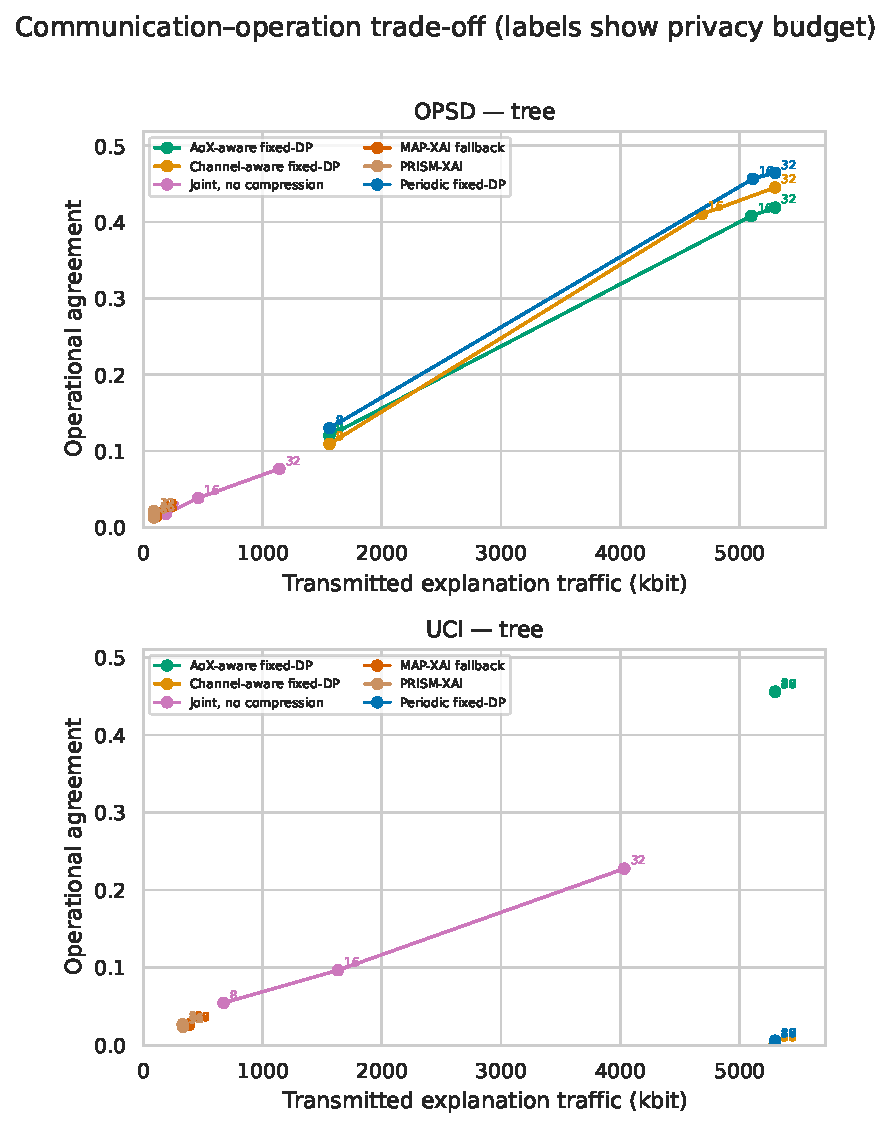
\includegraphics[width=.96\textwidth,height=.82\textheight,keepaspectratio]{../../SERVICE_TRADEOFF_RESULTS/runs/thr_0.5_cap_8/pareto_bits_fidelity.pdf}

\caption{Public-score threshold $\tau=0.5$, release cap $M=8$, Combined datasets: traffic--fidelity Pareto plane. This panel should be read with the setting-level quantitative interpretation and the complete tables immediately preceding the figure block.}

\end{figure*}

\clearpage

\begin{figure*}[p]

\centering

\includegraphics[width=.96\textwidth,height=.82\textheight,keepaspectratio]{../../SERVICE_TRADEOFF_RESULTS/runs/thr_0.5_cap_8/ablation_results.pdf}

\caption{Public-score threshold $\tau=0.5$, release cap $M=8$, Combined datasets: component ablation. This panel should be read with the setting-level quantitative interpretation and the complete tables immediately preceding the figure block.}

\end{figure*}

\clearpage

\paragraph{OPSD.} The three generated tables below report the full method means, all condition-level values, and paired differences. The five figures that follow provide the corresponding temporal, fairness, privacy, Pareto, and ablation views. Aggregate panels support the setting-level summary above; dataset panels reveal whether that summary is shared by OPSD and UCI rather than being driven by their different endpoint counts.

\begin{table*}[p]\centering\tiny

\caption{Public-score threshold $\tau=0.5$, release cap $M=8$, OPSD: complete generated method table.}

\label{tab:thr_0.5_cap_8:opsd:main}

\resizebox{\linewidth}{!}{% Values are means with 95% Student-t confidence intervals across seeds.
\begin{tabular}{lccccccccccccccc}
\toprule
Dataset & Model & $\epsilon_{\max}$ & Method & Top-$K$ & Cosine & Decision & Recall & Prec. & Abst. & P95 ms & kbit & Spent $\epsilon$ & False int. & bit/correct & Fairness \\
\midrule
OPSD & Tree & 8 & AoX-aware fixed-DP & 0.234 $\pm$ 0.048 & -0.033 $\pm$ 0.028 & 0.119 $\pm$ 0.028 & 0.119 $\pm$ 0.028 & 0.198 $\pm$ 0.054 & 0.721 $\pm$ 0.005 & 6.903 $\pm$ 1.126 & 1560.564 $\pm$ 0.000 & 7.990 $\pm$ 0.000 & 0.183 $\pm$ 0.020 & 35567.482 $\pm$ 10569.818 & 0.999 $\pm$ 0.000 \\
OPSD & Tree & 8 & AoX-aware fixed-DP & 0.238 $\pm$ 0.049 & -0.026 $\pm$ 0.055 & 0.121 $\pm$ 0.026 & 0.121 $\pm$ 0.026 & 0.205 $\pm$ 0.053 & 0.721 $\pm$ 0.005 & 6.903 $\pm$ 1.126 & 1560.564 $\pm$ 0.000 & 7.990 $\pm$ 0.000 & 0.179 $\pm$ 0.023 & 34123.214 $\pm$ 8376.542 & 0.999 $\pm$ 0.000 \\
OPSD & Tree & 8 & Channel-aware fixed-DP & 0.292 $\pm$ 0.037 & -0.041 $\pm$ 0.051 & 0.107 $\pm$ 0.026 & 0.107 $\pm$ 0.026 & 0.217 $\pm$ 0.068 & 0.779 $\pm$ 0.011 & 5.571 $\pm$ 1.784 & 1560.564 $\pm$ 0.000 & 7.990 $\pm$ 0.000 & 0.154 $\pm$ 0.029 & 40860.756 $\pm$ 14126.920 & 0.999 $\pm$ 0.000 \\
OPSD & Tree & 8 & Channel-aware fixed-DP & 0.292 $\pm$ 0.054 & -0.049 $\pm$ 0.064 & 0.111 $\pm$ 0.023 & 0.111 $\pm$ 0.023 & 0.228 $\pm$ 0.066 & 0.779 $\pm$ 0.011 & 5.571 $\pm$ 1.784 & 1560.564 $\pm$ 0.000 & 7.990 $\pm$ 0.000 & 0.149 $\pm$ 0.026 & 37980.855 $\pm$ 12338.094 & 0.999 $\pm$ 0.000 \\
OPSD & Tree & 8 & Joint, no compression & 0.288 $\pm$ 0.064 & -0.030 $\pm$ 0.079 & 0.016 $\pm$ 0.005 & 0.016 $\pm$ 0.005 & 0.193 $\pm$ 0.059 & 0.957 $\pm$ 0.003 & 4.560 $\pm$ 1.811 & 189.900 $\pm$ 0.554 & 7.990 $\pm$ 0.000 & 0.027 $\pm$ 0.005 & 32490.357 $\pm$ 10149.755 & 0.996 $\pm$ 0.002 \\
OPSD & Tree & 8 & Joint, no compression & 0.258 $\pm$ 0.055 & 0.011 $\pm$ 0.094 & 0.019 $\pm$ 0.004 & 0.019 $\pm$ 0.004 & 0.224 $\pm$ 0.044 & 0.957 $\pm$ 0.003 & 4.562 $\pm$ 1.809 & 189.750 $\pm$ 0.566 & 7.990 $\pm$ 0.000 & 0.025 $\pm$ 0.003 & 26079.167 $\pm$ 6335.386 & 0.996 $\pm$ 0.002 \\
OPSD & Tree & 8 & Periodic fixed-DP & 0.241 $\pm$ 0.049 & -0.019 $\pm$ 0.061 & 0.125 $\pm$ 0.020 & 0.125 $\pm$ 0.020 & 0.209 $\pm$ 0.044 & 0.722 $\pm$ 0.006 & 6.303 $\pm$ 1.438 & 1560.564 $\pm$ 0.000 & 7.990 $\pm$ 0.000 & 0.181 $\pm$ 0.021 & 31183.082 $\pm$ 4356.378 & 0.999 $\pm$ 0.000 \\
OPSD & Tree & 8 & Periodic fixed-DP & 0.242 $\pm$ 0.048 & -0.026 $\pm$ 0.082 & 0.135 $\pm$ 0.016 & 0.135 $\pm$ 0.016 & 0.231 $\pm$ 0.037 & 0.722 $\pm$ 0.006 & 6.303 $\pm$ 1.438 & 1560.564 $\pm$ 0.000 & 7.990 $\pm$ 0.000 & 0.169 $\pm$ 0.017 & 28520.235 $\pm$ 3511.595 & 0.999 $\pm$ 0.000 \\
OPSD & Tree & 8 & PRISM-XAI & 0.227 $\pm$ 0.040 & -0.036 $\pm$ 0.078 & 0.013 $\pm$ 0.005 & 0.013 $\pm$ 0.005 & 0.218 $\pm$ 0.087 & 0.964 $\pm$ 0.002 & 4.341 $\pm$ 1.447 & 87.697 $\pm$ 0.388 & 7.823 $\pm$ 0.000 & 0.018 $\pm$ 0.005 & 24929.927 $\pm$ 17099.604 & 0.993 $\pm$ 0.004 \\
OPSD & Tree & 8 & PRISM-XAI & 0.198 $\pm$ 0.035 & -0.021 $\pm$ 0.089 & 0.013 $\pm$ 0.005 & 0.013 $\pm$ 0.005 & 0.210 $\pm$ 0.097 & 0.964 $\pm$ 0.002 & 4.332 $\pm$ 1.445 & 87.461 $\pm$ 0.318 & 7.823 $\pm$ 0.000 & 0.019 $\pm$ 0.005 & 25702.427 $\pm$ 16465.572 & 0.993 $\pm$ 0.004 \\
OPSD & Tree & 8 & MAP-XAI fallback & 0.254 $\pm$ 0.049 & -0.070 $\pm$ 0.094 & 0.015 $\pm$ 0.005 & 0.015 $\pm$ 0.005 & 0.263 $\pm$ 0.086 & 0.964 $\pm$ 0.002 & 4.453 $\pm$ 1.383 & 105.817 $\pm$ 0.049 & 7.823 $\pm$ 0.000 & 0.016 $\pm$ 0.004 & 21748.429 $\pm$ 9602.332 & 0.993 $\pm$ 0.004 \\
OPSD & Tree & 8 & MAP-XAI fallback & 0.237 $\pm$ 0.043 & -0.048 $\pm$ 0.094 & 0.013 $\pm$ 0.006 & 0.013 $\pm$ 0.006 & 0.226 $\pm$ 0.081 & 0.964 $\pm$ 0.002 & 4.453 $\pm$ 1.383 & 105.675 $\pm$ 0.049 & 7.823 $\pm$ 0.000 & 0.017 $\pm$ 0.003 & 26069.368 $\pm$ 11426.445 & 0.993 $\pm$ 0.004 \\
\bottomrule
\end{tabular}
}

\end{table*}\clearpage

\begin{table*}[p]\centering\tiny

\caption{Public-score threshold $\tau=0.5$, release cap $M=8$, OPSD: complete condition-level generated table.}

\label{tab:thr_0.5_cap_8:opsd:conditions}

\resizebox{\textwidth}{!}{\begin{tabular}{llllccccccccccc}
\toprule
Dataset & Model & $\epsilon_{\max}$ & Method & kbit & Top-$K$ & Random Top-$K$ & Cosine & Decision & Recall & Precision & Coverage & Abstain & False int. & Spent $\epsilon$ \\
\midrule
OPSD & Tree & 8 & Joint, no compression & 189.900 $\pm$ 0.554 & 0.288 $\pm$ 0.064 & 0.250 $\pm$ 0.000 & -0.030 $\pm$ 0.079 & 0.016 $\pm$ 0.005 & 0.016 $\pm$ 0.005 & 0.193 $\pm$ 0.059 & 0.043 $\pm$ 0.003 & 0.957 $\pm$ 0.003 & 0.027 $\pm$ 0.005 & 7.990 $\pm$ 0.000 \\
OPSD & Tree & 8 & Joint, no compression & 189.750 $\pm$ 0.566 & 0.258 $\pm$ 0.055 & 0.250 $\pm$ 0.000 & 0.011 $\pm$ 0.094 & 0.019 $\pm$ 0.004 & 0.019 $\pm$ 0.004 & 0.224 $\pm$ 0.044 & 0.043 $\pm$ 0.003 & 0.957 $\pm$ 0.003 & 0.025 $\pm$ 0.003 & 7.990 $\pm$ 0.000 \\
OPSD & Tree & 8 & Periodic fixed-DP & 1560.564 $\pm$ 0.000 & 0.241 $\pm$ 0.049 & 0.250 $\pm$ 0.000 & -0.019 $\pm$ 0.061 & 0.125 $\pm$ 0.020 & 0.125 $\pm$ 0.020 & 0.209 $\pm$ 0.044 & 0.278 $\pm$ 0.006 & 0.722 $\pm$ 0.006 & 0.181 $\pm$ 0.021 & 7.990 $\pm$ 0.000 \\
OPSD & Tree & 8 & Periodic fixed-DP & 1560.564 $\pm$ 0.000 & 0.242 $\pm$ 0.048 & 0.250 $\pm$ 0.000 & -0.026 $\pm$ 0.082 & 0.135 $\pm$ 0.016 & 0.135 $\pm$ 0.016 & 0.231 $\pm$ 0.037 & 0.278 $\pm$ 0.006 & 0.722 $\pm$ 0.006 & 0.169 $\pm$ 0.017 & 7.990 $\pm$ 0.000 \\
OPSD & Tree & 8 & PRISM-XAI & 87.697 $\pm$ 0.388 & 0.227 $\pm$ 0.040 & 0.250 $\pm$ 0.000 & -0.036 $\pm$ 0.078 & 0.013 $\pm$ 0.005 & 0.013 $\pm$ 0.005 & 0.218 $\pm$ 0.087 & 0.036 $\pm$ 0.002 & 0.964 $\pm$ 0.002 & 0.018 $\pm$ 0.005 & 7.823 $\pm$ 0.000 \\
OPSD & Tree & 8 & PRISM-XAI & 87.461 $\pm$ 0.318 & 0.198 $\pm$ 0.035 & 0.250 $\pm$ 0.000 & -0.021 $\pm$ 0.089 & 0.013 $\pm$ 0.005 & 0.013 $\pm$ 0.005 & 0.210 $\pm$ 0.097 & 0.036 $\pm$ 0.002 & 0.964 $\pm$ 0.002 & 0.019 $\pm$ 0.005 & 7.823 $\pm$ 0.000 \\
OPSD & Tree & 16 & Joint, no compression & 459.900 $\pm$ 0.750 & 0.232 $\pm$ 0.065 & 0.250 $\pm$ 0.000 & 0.059 $\pm$ 0.048 & 0.038 $\pm$ 0.009 & 0.038 $\pm$ 0.009 & 0.222 $\pm$ 0.049 & 0.088 $\pm$ 0.004 & 0.912 $\pm$ 0.004 & 0.049 $\pm$ 0.005 & 15.997 $\pm$ 0.000 \\
OPSD & Tree & 16 & Joint, no compression & 460.050 $\pm$ 0.724 & 0.241 $\pm$ 0.055 & 0.250 $\pm$ 0.000 & 0.061 $\pm$ 0.052 & 0.039 $\pm$ 0.008 & 0.039 $\pm$ 0.008 & 0.241 $\pm$ 0.042 & 0.088 $\pm$ 0.004 & 0.912 $\pm$ 0.004 & 0.045 $\pm$ 0.004 & 15.997 $\pm$ 0.000 \\
OPSD & Tree & 16 & Periodic fixed-DP & 5112.594 $\pm$ 0.000 & 0.249 $\pm$ 0.022 & 0.250 $\pm$ 0.000 & -0.009 $\pm$ 0.045 & 0.450 $\pm$ 0.062 & 0.450 $\pm$ 0.062 & 0.237 $\pm$ 0.042 & 0.985 $\pm$ 0.002 & 0.015 $\pm$ 0.002 & 0.551 $\pm$ 0.057 & 15.997 $\pm$ 0.000 \\
OPSD & Tree & 16 & Periodic fixed-DP & 5112.594 $\pm$ 0.000 & 0.243 $\pm$ 0.019 & 0.250 $\pm$ 0.000 & -0.012 $\pm$ 0.050 & 0.463 $\pm$ 0.047 & 0.463 $\pm$ 0.047 & 0.240 $\pm$ 0.028 & 0.985 $\pm$ 0.002 & 0.015 $\pm$ 0.002 & 0.547 $\pm$ 0.036 & 15.997 $\pm$ 0.000 \\
OPSD & Tree & 16 & PRISM-XAI & 87.635 $\pm$ 0.376 & 0.225 $\pm$ 0.047 & 0.250 $\pm$ 0.000 & 0.065 $\pm$ 0.050 & 0.016 $\pm$ 0.004 & 0.016 $\pm$ 0.004 & 0.293 $\pm$ 0.081 & 0.036 $\pm$ 0.002 & 0.964 $\pm$ 0.002 & 0.015 $\pm$ 0.004 & 15.620 $\pm$ 0.000 \\
OPSD & Tree & 16 & PRISM-XAI & 87.431 $\pm$ 0.305 & 0.188 $\pm$ 0.051 & 0.250 $\pm$ 0.000 & 0.103 $\pm$ 0.067 & 0.017 $\pm$ 0.005 & 0.017 $\pm$ 0.005 & 0.302 $\pm$ 0.076 & 0.036 $\pm$ 0.002 & 0.964 $\pm$ 0.002 & 0.015 $\pm$ 0.004 & 15.620 $\pm$ 0.000 \\
OPSD & Tree & 32 & Joint, no compression & 1140.900 $\pm$ 7.953 & 0.235 $\pm$ 0.064 & 0.250 $\pm$ 0.000 & -0.031 $\pm$ 0.089 & 0.074 $\pm$ 0.015 & 0.074 $\pm$ 0.015 & 0.205 $\pm$ 0.039 & 0.157 $\pm$ 0.006 & 0.843 $\pm$ 0.006 & 0.107 $\pm$ 0.009 & 31.999 $\pm$ 0.000 \\
OPSD & Tree & 32 & Joint, no compression & 1140.900 $\pm$ 7.953 & 0.282 $\pm$ 0.054 & 0.250 $\pm$ 0.000 & -0.044 $\pm$ 0.076 & 0.080 $\pm$ 0.011 & 0.080 $\pm$ 0.011 & 0.227 $\pm$ 0.052 & 0.158 $\pm$ 0.006 & 0.842 $\pm$ 0.006 & 0.105 $\pm$ 0.015 & 31.999 $\pm$ 0.000 \\
OPSD & Tree & 32 & Periodic fixed-DP & 5299.836 $\pm$ 0.625 & 0.249 $\pm$ 0.022 & 0.250 $\pm$ 0.000 & -0.009 $\pm$ 0.044 & 0.458 $\pm$ 0.066 & 0.458 $\pm$ 0.066 & 0.237 $\pm$ 0.045 & 1.000 $\pm$ 0.000 & 0.000 $\pm$ 0.000 & 0.562 $\pm$ 0.062 & 16.371 $\pm$ 0.000 \\
OPSD & Tree & 32 & Periodic fixed-DP & 5299.836 $\pm$ 0.625 & 0.244 $\pm$ 0.019 & 0.250 $\pm$ 0.000 & -0.012 $\pm$ 0.050 & 0.471 $\pm$ 0.049 & 0.471 $\pm$ 0.049 & 0.240 $\pm$ 0.029 & 1.000 $\pm$ 0.000 & 0.000 $\pm$ 0.000 & 0.559 $\pm$ 0.039 & 16.371 $\pm$ 0.000 \\
OPSD & Tree & 32 & PRISM-XAI & 87.574 $\pm$ 0.349 & 0.335 $\pm$ 0.044 & 0.250 $\pm$ 0.000 & 0.205 $\pm$ 0.062 & 0.020 $\pm$ 0.003 & 0.020 $\pm$ 0.003 & 0.478 $\pm$ 0.125 & 0.036 $\pm$ 0.002 & 0.964 $\pm$ 0.002 & 0.010 $\pm$ 0.004 & 31.175 $\pm$ 0.000 \\
OPSD & Tree & 32 & PRISM-XAI & 87.216 $\pm$ 0.281 & 0.311 $\pm$ 0.061 & 0.250 $\pm$ 0.000 & 0.292 $\pm$ 0.078 & 0.022 $\pm$ 0.004 & 0.022 $\pm$ 0.004 & 0.495 $\pm$ 0.133 & 0.036 $\pm$ 0.002 & 0.964 $\pm$ 0.002 & 0.009 $\pm$ 0.004 & 31.175 $\pm$ 0.000 \\
\bottomrule
\end{tabular}
}

\end{table*}\clearpage

\begin{table*}[p]\centering\tiny

\caption{Public-score threshold $\tau=0.5$, release cap $M=8$, OPSD: complete generated paired comparisons.}

\label{tab:thr_0.5_cap_8:opsd:paired}

\resizebox{\textwidth}{!}{\begin{tabular}{llcccc}
\toprule
Dataset & Baseline & Delta kbit & Delta Top-$K$ & Delta recall & Delta fairness \\
\midrule
OPSD & AoX-aware fixed-DP & -1472.867 $\pm$ 0.388 & -0.007 $\pm$ 0.067 & -0.106 $\pm$ 0.030 & -0.007 $\pm$ 0.003 \\
OPSD & AoX-aware fixed-DP & -5012.277 $\pm$ 5.554 & -0.029 $\pm$ 0.038 & -0.385 $\pm$ 0.074 & -0.007 $\pm$ 0.004 \\
OPSD & AoX-aware fixed-DP & -5212.650 $\pm$ 0.349 & 0.082 $\pm$ 0.065 & -0.392 $\pm$ 0.079 & -0.007 $\pm$ 0.004 \\
OPSD & AoX-aware fixed-DP & -1473.103 $\pm$ 0.318 & -0.040 $\pm$ 0.037 & -0.108 $\pm$ 0.027 & -0.007 $\pm$ 0.003 \\
OPSD & AoX-aware fixed-DP & -5012.482 $\pm$ 5.458 & -0.064 $\pm$ 0.038 & -0.397 $\pm$ 0.056 & -0.007 $\pm$ 0.004 \\
OPSD & AoX-aware fixed-DP & -5213.008 $\pm$ 0.281 & 0.060 $\pm$ 0.073 & -0.403 $\pm$ 0.058 & -0.006 $\pm$ 0.004 \\
OPSD & Channel-aware fixed-DP & -1472.867 $\pm$ 0.388 & -0.066 $\pm$ 0.052 & -0.094 $\pm$ 0.027 & -0.007 $\pm$ 0.003 \\
OPSD & Channel-aware fixed-DP & -4598.974 $\pm$ 13.023 & -0.037 $\pm$ 0.042 & -0.385 $\pm$ 0.089 & 0.055 $\pm$ 0.005 \\
OPSD & Channel-aware fixed-DP & -5212.650 $\pm$ 0.349 & 0.077 $\pm$ 0.057 & -0.414 $\pm$ 0.099 & 0.086 $\pm$ 0.006 \\
OPSD & Channel-aware fixed-DP & -1473.103 $\pm$ 0.318 & -0.094 $\pm$ 0.052 & -0.098 $\pm$ 0.023 & -0.007 $\pm$ 0.003 \\
OPSD & Channel-aware fixed-DP & -4599.179 $\pm$ 12.890 & -0.070 $\pm$ 0.045 & -0.402 $\pm$ 0.087 & 0.056 $\pm$ 0.006 \\
OPSD & Channel-aware fixed-DP & -5213.008 $\pm$ 0.281 & 0.054 $\pm$ 0.072 & -0.434 $\pm$ 0.091 & 0.086 $\pm$ 0.007 \\
OPSD & Joint, no compression & -102.203 $\pm$ 0.557 & -0.061 $\pm$ 0.073 & -0.003 $\pm$ 0.004 & -0.003 $\pm$ 0.003 \\
OPSD & Joint, no compression & -372.265 $\pm$ 1.026 & -0.007 $\pm$ 0.078 & -0.022 $\pm$ 0.008 & -0.005 $\pm$ 0.004 \\
OPSD & Joint, no compression & -1053.326 $\pm$ 8.018 & 0.100 $\pm$ 0.086 & -0.053 $\pm$ 0.014 & -0.006 $\pm$ 0.004 \\
OPSD & Joint, no compression & -102.289 $\pm$ 0.585 & -0.060 $\pm$ 0.065 & -0.006 $\pm$ 0.004 & -0.003 $\pm$ 0.003 \\
OPSD & Joint, no compression & -372.619 $\pm$ 0.786 & -0.052 $\pm$ 0.062 & -0.022 $\pm$ 0.008 & -0.004 $\pm$ 0.004 \\
OPSD & Joint, no compression & -1053.684 $\pm$ 7.938 & 0.030 $\pm$ 0.075 & -0.058 $\pm$ 0.011 & -0.006 $\pm$ 0.004 \\
OPSD & Periodic fixed-DP & -1472.867 $\pm$ 0.388 & -0.014 $\pm$ 0.067 & -0.112 $\pm$ 0.022 & -0.007 $\pm$ 0.004 \\
OPSD & Periodic fixed-DP & -5024.959 $\pm$ 0.376 & -0.024 $\pm$ 0.047 & -0.434 $\pm$ 0.062 & -0.007 $\pm$ 0.004 \\
OPSD & Periodic fixed-DP & -5212.262 $\pm$ 0.599 & 0.086 $\pm$ 0.047 & -0.438 $\pm$ 0.067 & -0.007 $\pm$ 0.004 \\
OPSD & Periodic fixed-DP & -1473.103 $\pm$ 0.318 & -0.044 $\pm$ 0.028 & -0.122 $\pm$ 0.018 & -0.007 $\pm$ 0.004 \\
OPSD & Periodic fixed-DP & -5025.163 $\pm$ 0.305 & -0.055 $\pm$ 0.045 & -0.445 $\pm$ 0.049 & -0.007 $\pm$ 0.004 \\
OPSD & Periodic fixed-DP & -5212.620 $\pm$ 0.569 & 0.068 $\pm$ 0.064 & -0.449 $\pm$ 0.049 & -0.007 $\pm$ 0.004 \\
OPSD & MAP-XAI fallback & -18.120 $\pm$ 0.382 & -0.028 $\pm$ 0.044 & -0.002 $\pm$ 0.004 & 0.000 $\pm$ 0.000 \\
OPSD & MAP-XAI fallback & -18.181 $\pm$ 0.373 & -0.017 $\pm$ 0.079 & -0.000 $\pm$ 0.004 & 0.000 $\pm$ 0.000 \\
OPSD & MAP-XAI fallback & -18.243 $\pm$ 0.359 & -0.030 $\pm$ 0.076 & 0.001 $\pm$ 0.004 & -0.000 $\pm$ 0.000 \\
OPSD & MAP-XAI fallback & -18.214 $\pm$ 0.313 & -0.038 $\pm$ 0.052 & -0.001 $\pm$ 0.004 & 0.000 $\pm$ 0.000 \\
OPSD & MAP-XAI fallback & -18.203 $\pm$ 0.325 & -0.043 $\pm$ 0.051 & 0.001 $\pm$ 0.005 & 0.001 $\pm$ 0.001 \\
OPSD & MAP-XAI fallback & -18.315 $\pm$ 0.369 & -0.005 $\pm$ 0.066 & 0.002 $\pm$ 0.003 & 0.000 $\pm$ 0.000 \\
\bottomrule
\end{tabular}
}

\end{table*}\clearpage

\begin{figure*}[p]

\centering

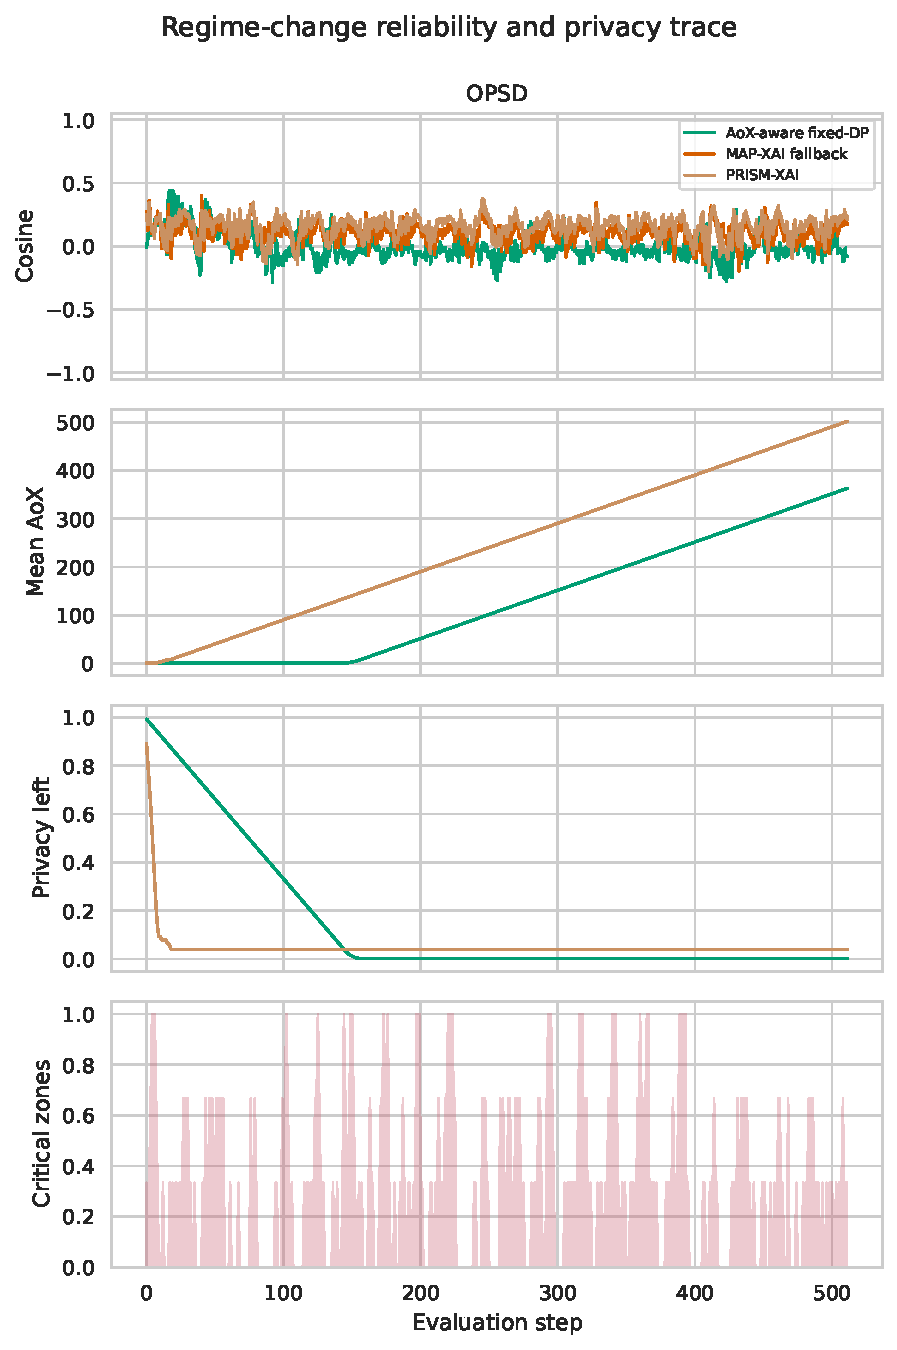
\includegraphics[width=.96\textwidth,height=.82\textheight,keepaspectratio]{../../SERVICE_TRADEOFF_RESULTS/runs/thr_0.5_cap_8/opsd/regime_trace.pdf}

\caption{Public-score threshold $\tau=0.5$, release cap $M=8$, OPSD: representative regime trace. This panel should be read with the setting-level quantitative interpretation and the complete tables immediately preceding the figure block.}

\end{figure*}

\clearpage

\begin{figure*}[p]

\centering

\includegraphics[width=.96\textwidth,height=.82\textheight,keepaspectratio]{../../SERVICE_TRADEOFF_RESULTS/runs/thr_0.5_cap_8/opsd/fairness_reliability.pdf}

\caption{Public-score threshold $\tau=0.5$, release cap $M=8$, OPSD: fairness--reliability plane. This panel should be read with the setting-level quantitative interpretation and the complete tables immediately preceding the figure block.}

\end{figure*}

\clearpage

\begin{figure*}[p]

\centering

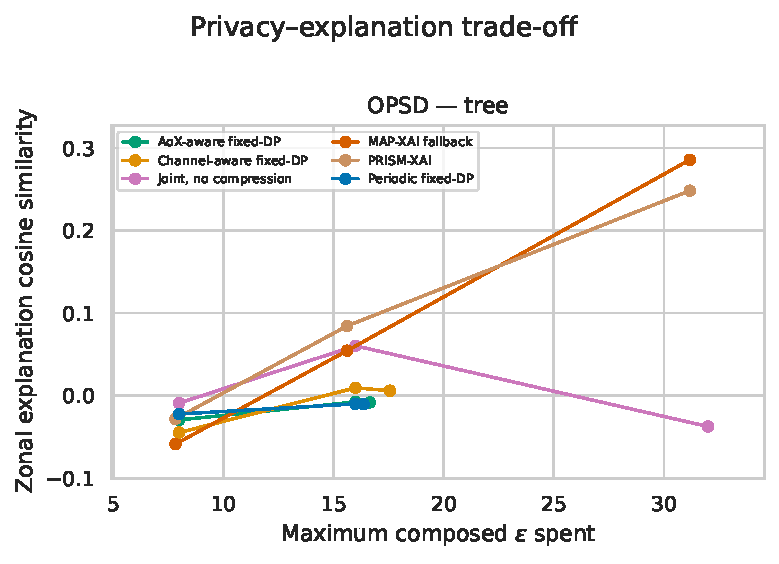
\includegraphics[width=.96\textwidth,height=.82\textheight,keepaspectratio]{../../SERVICE_TRADEOFF_RESULTS/runs/thr_0.5_cap_8/opsd/privacy_fidelity.pdf}

\caption{Public-score threshold $\tau=0.5$, release cap $M=8$, OPSD: privacy--fidelity plane. This panel should be read with the setting-level quantitative interpretation and the complete tables immediately preceding the figure block.}

\end{figure*}

\clearpage

\begin{figure*}[p]

\centering

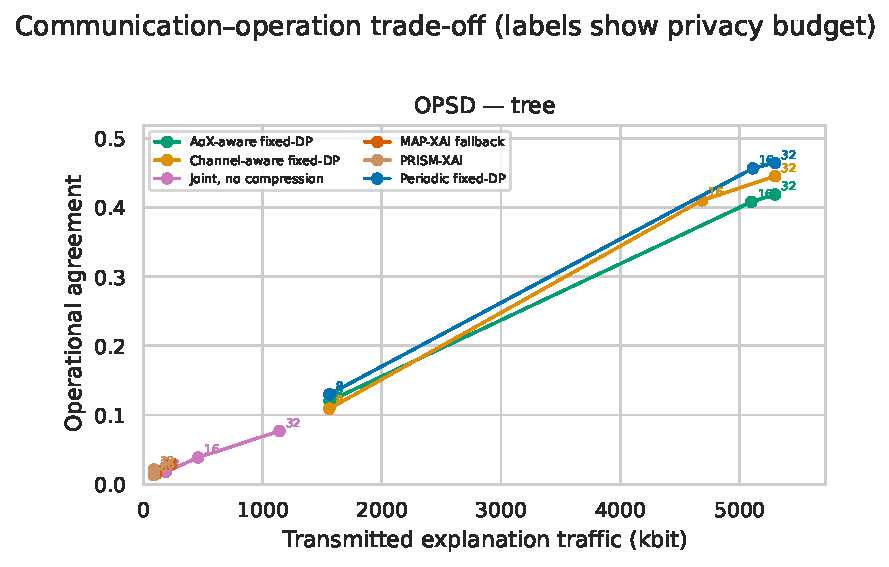
\includegraphics[width=.96\textwidth,height=.82\textheight,keepaspectratio]{../../SERVICE_TRADEOFF_RESULTS/runs/thr_0.5_cap_8/opsd/pareto_bits_fidelity.pdf}

\caption{Public-score threshold $\tau=0.5$, release cap $M=8$, OPSD: traffic--fidelity Pareto plane. This panel should be read with the setting-level quantitative interpretation and the complete tables immediately preceding the figure block.}

\end{figure*}

\clearpage

\begin{figure*}[p]

\centering

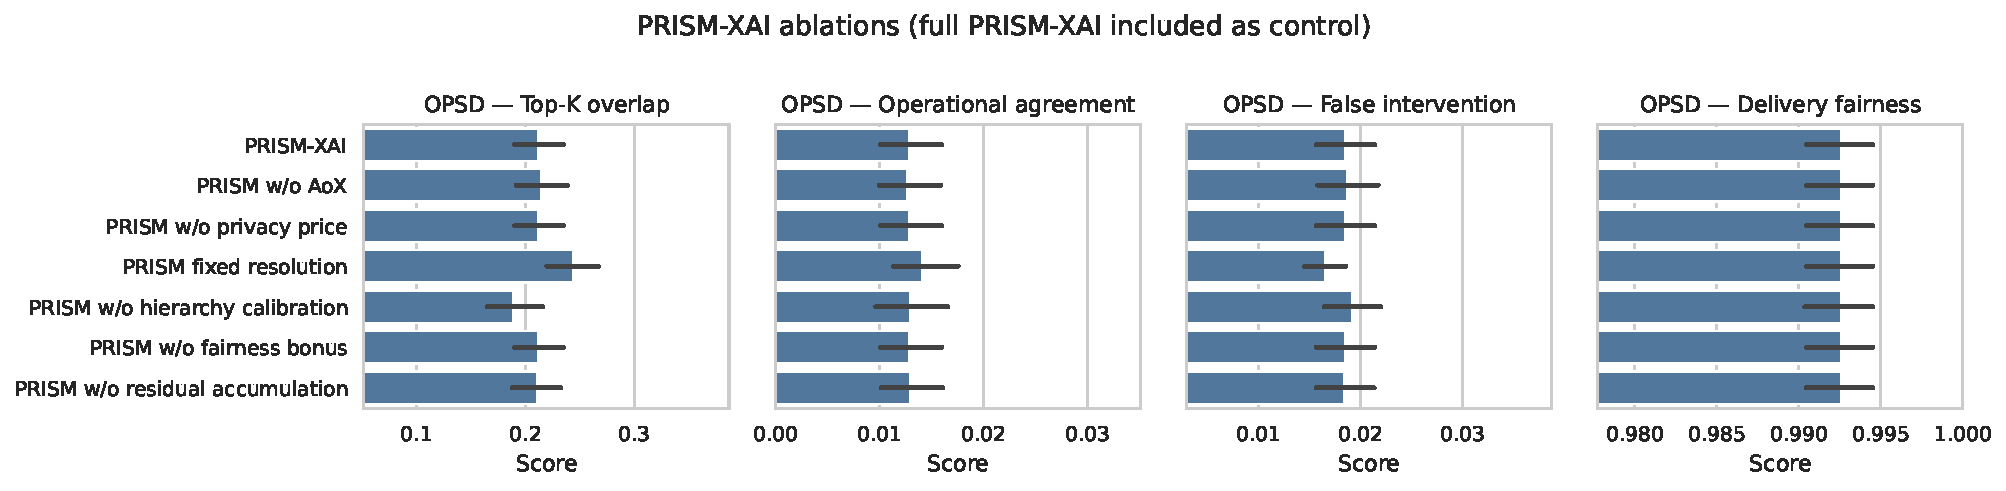
\includegraphics[width=.96\textwidth,height=.82\textheight,keepaspectratio]{../../SERVICE_TRADEOFF_RESULTS/runs/thr_0.5_cap_8/opsd/ablation_results.pdf}

\caption{Public-score threshold $\tau=0.5$, release cap $M=8$, OPSD: component ablation. This panel should be read with the setting-level quantitative interpretation and the complete tables immediately preceding the figure block.}

\end{figure*}

\clearpage

\paragraph{UCI.} The three generated tables below report the full method means, all condition-level values, and paired differences. The five figures that follow provide the corresponding temporal, fairness, privacy, Pareto, and ablation views. Aggregate panels support the setting-level summary above; dataset panels reveal whether that summary is shared by OPSD and UCI rather than being driven by their different endpoint counts.

\begin{table*}[p]\centering\tiny

\caption{Public-score threshold $\tau=0.5$, release cap $M=8$, UCI: complete generated method table.}

\label{tab:thr_0.5_cap_8:uci:main}

\resizebox{\linewidth}{!}{% Values are means with 95% Student-t confidence intervals across seeds.
\begin{tabular}{lccccccccccccccc}
\toprule
Dataset & Model & $\epsilon_{\max}$ & Method & Top-$K$ & Cosine & Decision & Recall & Prec. & Abst. & P95 ms & kbit & Spent $\epsilon$ & False int. & bit/correct & Fairness \\
\midrule
UCI & Tree & 8 & AoX-aware fixed-DP & 0.263 $\pm$ 0.041 & -0.007 $\pm$ 0.009 & 0.457 $\pm$ 0.031 & 0.457 $\pm$ 0.031 & 0.362 $\pm$ 0.024 & 0.003 $\pm$ 0.001 & 7.500 $\pm$ 0.000 & 5300.224 $\pm$ 0.000 & 7.990 $\pm$ 0.000 & 0.557 $\pm$ 0.025 & 14002.896 $\pm$ 1040.243 & 0.999 $\pm$ 0.000 \\
UCI & Tree & 8 & AoX-aware fixed-DP & 0.260 $\pm$ 0.022 & 0.010 $\pm$ 0.055 & 0.455 $\pm$ 0.047 & 0.455 $\pm$ 0.047 & 0.361 $\pm$ 0.038 & 0.003 $\pm$ 0.001 & 7.500 $\pm$ 0.000 & 5300.224 $\pm$ 0.000 & 7.990 $\pm$ 0.000 & 0.557 $\pm$ 0.048 & 14198.303 $\pm$ 1508.274 & 0.999 $\pm$ 0.000 \\
UCI & Tree & 8 & Channel-aware fixed-DP & 0.248 $\pm$ 0.031 & 0.004 $\pm$ 0.012 & 0.001 $\pm$ 0.001 & 0.001 $\pm$ 0.001 & 0.150 $\pm$ 0.151 & 0.999 $\pm$ 0.001 & 4.609 $\pm$ 1.781 & 5295.177 $\pm$ 3.740 & 7.990 $\pm$ 0.000 & 0.001 $\pm$ 0.001 & 4632196.500 $\pm$ 2102650.252 & 0.991 $\pm$ 0.001 \\
UCI & Tree & 8 & Channel-aware fixed-DP & 0.239 $\pm$ 0.030 & -0.020 $\pm$ 0.055 & 0.000 $\pm$ 0.000 & 0.000 $\pm$ 0.000 & 0.117 $\pm$ 0.225 & 0.999 $\pm$ 0.001 & 4.609 $\pm$ 1.781 & 5295.177 $\pm$ 3.740 & 7.990 $\pm$ 0.000 & 0.001 $\pm$ 0.001 & 5296989.000 $\pm$ 41104.572 & 0.991 $\pm$ 0.001 \\
UCI & Tree & 8 & Joint, no compression & 0.286 $\pm$ 0.045 & 0.004 $\pm$ 0.020 & 0.052 $\pm$ 0.005 & 0.052 $\pm$ 0.005 & 0.406 $\pm$ 0.037 & 0.875 $\pm$ 0.003 & 5.123 $\pm$ 1.792 & 672.300 $\pm$ 0.452 & 7.990 $\pm$ 0.000 & 0.053 $\pm$ 0.004 & 15676.175 $\pm$ 1475.621 & 0.994 $\pm$ 0.003 \\
UCI & Tree & 8 & Joint, no compression & 0.229 $\pm$ 0.052 & -0.032 $\pm$ 0.050 & 0.057 $\pm$ 0.007 & 0.057 $\pm$ 0.007 & 0.428 $\pm$ 0.041 & 0.875 $\pm$ 0.003 & 5.131 $\pm$ 1.787 & 672.300 $\pm$ 0.452 & 7.990 $\pm$ 0.000 & 0.052 $\pm$ 0.004 & 14702.786 $\pm$ 2334.488 & 0.994 $\pm$ 0.003 \\
UCI & Tree & 8 & Periodic fixed-DP & 0.259 $\pm$ 0.060 & -0.005 $\pm$ 0.008 & 0.006 $\pm$ 0.001 & 0.006 $\pm$ 0.001 & 0.244 $\pm$ 0.049 & 0.989 $\pm$ 0.001 & 4.596 $\pm$ 1.788 & 5299.318 $\pm$ 1.451 & 7.786 $\pm$ 0.000 & 0.013 $\pm$ 0.002 & 1215103.896 $\pm$ 390671.319 & 0.999 $\pm$ 0.000 \\
UCI & Tree & 8 & Periodic fixed-DP & 0.260 $\pm$ 0.044 & 0.022 $\pm$ 0.070 & 0.005 $\pm$ 0.001 & 0.005 $\pm$ 0.001 & 0.195 $\pm$ 0.050 & 0.989 $\pm$ 0.001 & 4.596 $\pm$ 1.788 & 5299.318 $\pm$ 1.451 & 7.786 $\pm$ 0.000 & 0.015 $\pm$ 0.002 & 1555837.203 $\pm$ 955472.503 & 0.999 $\pm$ 0.000 \\
UCI & Tree & 8 & PRISM-XAI & 0.238 $\pm$ 0.091 & 0.008 $\pm$ 0.022 & 0.028 $\pm$ 0.004 & 0.028 $\pm$ 0.004 & 0.465 $\pm$ 0.035 & 0.940 $\pm$ 0.003 & 4.723 $\pm$ 1.732 & 330.248 $\pm$ 1.899 & 7.823 $\pm$ 0.000 & 0.022 $\pm$ 0.002 & 14725.609 $\pm$ 2267.563 & 0.991 $\pm$ 0.003 \\
UCI & Tree & 8 & PRISM-XAI & 0.233 $\pm$ 0.050 & -0.032 $\pm$ 0.070 & 0.026 $\pm$ 0.003 & 0.026 $\pm$ 0.003 & 0.454 $\pm$ 0.085 & 0.945 $\pm$ 0.005 & 4.249 $\pm$ 1.633 & 327.398 $\pm$ 2.091 & 7.823 $\pm$ 0.000 & 0.022 $\pm$ 0.005 & 15910.590 $\pm$ 2766.316 & 0.991 $\pm$ 0.004 \\
UCI & Tree & 8 & MAP-XAI fallback & 0.224 $\pm$ 0.053 & 0.017 $\pm$ 0.017 & 0.027 $\pm$ 0.005 & 0.027 $\pm$ 0.005 & 0.459 $\pm$ 0.057 & 0.940 $\pm$ 0.003 & 4.895 $\pm$ 1.639 & 382.160 $\pm$ 0.072 & 7.823 $\pm$ 0.000 & 0.021 $\pm$ 0.002 & 17976.663 $\pm$ 3232.835 & 0.990 $\pm$ 0.003 \\
UCI & Tree & 8 & MAP-XAI fallback & 0.251 $\pm$ 0.037 & -0.011 $\pm$ 0.080 & 0.026 $\pm$ 0.006 & 0.026 $\pm$ 0.006 & 0.462 $\pm$ 0.081 & 0.943 $\pm$ 0.006 & 5.591 $\pm$ 1.764 & 381.645 $\pm$ 0.090 & 7.823 $\pm$ 0.000 & 0.021 $\pm$ 0.005 & 18792.055 $\pm$ 3629.218 & 0.989 $\pm$ 0.004 \\
\bottomrule
\end{tabular}
}

\end{table*}\clearpage

\begin{table*}[p]\centering\tiny

\caption{Public-score threshold $\tau=0.5$, release cap $M=8$, UCI: complete condition-level generated table.}

\label{tab:thr_0.5_cap_8:uci:conditions}

\resizebox{\textwidth}{!}{\begin{tabular}{llllccccccccccc}
\toprule
Dataset & Model & $\epsilon_{\max}$ & Method & kbit & Top-$K$ & Random Top-$K$ & Cosine & Decision & Recall & Precision & Coverage & Abstain & False int. & Spent $\epsilon$ \\
\midrule
UCI & Tree & 8 & Joint, no compression & 672.300 $\pm$ 0.452 & 0.286 $\pm$ 0.045 & 0.250 $\pm$ 0.000 & 0.004 $\pm$ 0.020 & 0.052 $\pm$ 0.005 & 0.052 $\pm$ 0.005 & 0.406 $\pm$ 0.037 & 0.125 $\pm$ 0.003 & 0.875 $\pm$ 0.003 & 0.053 $\pm$ 0.004 & 7.990 $\pm$ 0.000 \\
UCI & Tree & 8 & Joint, no compression & 672.300 $\pm$ 0.452 & 0.229 $\pm$ 0.052 & 0.250 $\pm$ 0.000 & -0.032 $\pm$ 0.050 & 0.057 $\pm$ 0.007 & 0.057 $\pm$ 0.007 & 0.428 $\pm$ 0.041 & 0.125 $\pm$ 0.003 & 0.875 $\pm$ 0.003 & 0.052 $\pm$ 0.004 & 7.990 $\pm$ 0.000 \\
UCI & Tree & 8 & Periodic fixed-DP & 5299.318 $\pm$ 1.451 & 0.259 $\pm$ 0.060 & 0.250 $\pm$ 0.000 & -0.005 $\pm$ 0.008 & 0.006 $\pm$ 0.001 & 0.006 $\pm$ 0.001 & 0.244 $\pm$ 0.049 & 0.011 $\pm$ 0.001 & 0.989 $\pm$ 0.001 & 0.013 $\pm$ 0.002 & 7.786 $\pm$ 0.000 \\
UCI & Tree & 8 & Periodic fixed-DP & 5299.318 $\pm$ 1.451 & 0.260 $\pm$ 0.044 & 0.250 $\pm$ 0.000 & 0.022 $\pm$ 0.070 & 0.005 $\pm$ 0.001 & 0.005 $\pm$ 0.001 & 0.195 $\pm$ 0.050 & 0.011 $\pm$ 0.001 & 0.989 $\pm$ 0.001 & 0.015 $\pm$ 0.002 & 7.786 $\pm$ 0.000 \\
UCI & Tree & 8 & PRISM-XAI & 330.248 $\pm$ 1.899 & 0.238 $\pm$ 0.091 & 0.250 $\pm$ 0.000 & 0.008 $\pm$ 0.022 & 0.028 $\pm$ 0.004 & 0.028 $\pm$ 0.004 & 0.465 $\pm$ 0.035 & 0.060 $\pm$ 0.003 & 0.940 $\pm$ 0.003 & 0.022 $\pm$ 0.002 & 7.823 $\pm$ 0.000 \\
UCI & Tree & 8 & PRISM-XAI & 327.398 $\pm$ 2.091 & 0.233 $\pm$ 0.050 & 0.250 $\pm$ 0.000 & -0.032 $\pm$ 0.070 & 0.026 $\pm$ 0.003 & 0.026 $\pm$ 0.003 & 0.454 $\pm$ 0.085 & 0.055 $\pm$ 0.005 & 0.945 $\pm$ 0.005 & 0.022 $\pm$ 0.005 & 7.823 $\pm$ 0.000 \\
UCI & Tree & 16 & Joint, no compression & 1632.150 $\pm$ 0.339 & 0.216 $\pm$ 0.041 & 0.250 $\pm$ 0.000 & 0.001 $\pm$ 0.012 & 0.094 $\pm$ 0.005 & 0.094 $\pm$ 0.005 & 0.330 $\pm$ 0.024 & 0.228 $\pm$ 0.005 & 0.772 $\pm$ 0.005 & 0.133 $\pm$ 0.010 & 15.997 $\pm$ 0.000 \\
UCI & Tree & 16 & Joint, no compression & 1632.600 $\pm$ 0.554 & 0.204 $\pm$ 0.011 & 0.250 $\pm$ 0.000 & -0.021 $\pm$ 0.033 & 0.099 $\pm$ 0.016 & 0.099 $\pm$ 0.016 & 0.347 $\pm$ 0.054 & 0.228 $\pm$ 0.005 & 0.772 $\pm$ 0.005 & 0.128 $\pm$ 0.011 & 15.997 $\pm$ 0.000 \\
UCI & Tree & 16 & Periodic fixed-DP & 5299.318 $\pm$ 1.451 & 0.259 $\pm$ 0.060 & 0.250 $\pm$ 0.000 & -0.005 $\pm$ 0.008 & 0.006 $\pm$ 0.001 & 0.006 $\pm$ 0.001 & 0.244 $\pm$ 0.049 & 0.011 $\pm$ 0.001 & 0.989 $\pm$ 0.001 & 0.013 $\pm$ 0.002 & 7.786 $\pm$ 0.000 \\
UCI & Tree & 16 & Periodic fixed-DP & 5299.318 $\pm$ 1.451 & 0.260 $\pm$ 0.044 & 0.250 $\pm$ 0.000 & 0.022 $\pm$ 0.070 & 0.005 $\pm$ 0.001 & 0.005 $\pm$ 0.001 & 0.195 $\pm$ 0.050 & 0.011 $\pm$ 0.001 & 0.989 $\pm$ 0.001 & 0.015 $\pm$ 0.002 & 7.786 $\pm$ 0.000 \\
UCI & Tree & 16 & PRISM-XAI & 330.309 $\pm$ 1.645 & 0.201 $\pm$ 0.066 & 0.250 $\pm$ 0.000 & 0.022 $\pm$ 0.015 & 0.027 $\pm$ 0.005 & 0.027 $\pm$ 0.005 & 0.573 $\pm$ 0.085 & 0.058 $\pm$ 0.004 & 0.942 $\pm$ 0.004 & 0.015 $\pm$ 0.004 & 15.620 $\pm$ 0.000 \\
UCI & Tree & 16 & PRISM-XAI & 329.517 $\pm$ 1.193 & 0.267 $\pm$ 0.020 & 0.250 $\pm$ 0.000 & 0.044 $\pm$ 0.071 & 0.022 $\pm$ 0.003 & 0.022 $\pm$ 0.003 & 0.521 $\pm$ 0.092 & 0.048 $\pm$ 0.004 & 0.952 $\pm$ 0.004 & 0.015 $\pm$ 0.005 & 15.620 $\pm$ 0.000 \\
UCI & Tree & 32 & Joint, no compression & 4034.550 $\pm$ 5.034 & 0.246 $\pm$ 0.031 & 0.250 $\pm$ 0.000 & -0.002 $\pm$ 0.015 & 0.228 $\pm$ 0.013 & 0.228 $\pm$ 0.013 & 0.361 $\pm$ 0.028 & 0.537 $\pm$ 0.009 & 0.463 $\pm$ 0.009 & 0.279 $\pm$ 0.017 & 31.999 $\pm$ 0.000 \\
UCI & Tree & 32 & Joint, no compression & 4034.550 $\pm$ 5.034 & 0.241 $\pm$ 0.033 & 0.250 $\pm$ 0.000 & -0.012 $\pm$ 0.030 & 0.228 $\pm$ 0.028 & 0.228 $\pm$ 0.028 & 0.360 $\pm$ 0.047 & 0.530 $\pm$ 0.010 & 0.470 $\pm$ 0.010 & 0.280 $\pm$ 0.026 & 31.999 $\pm$ 0.000 \\
UCI & Tree & 32 & Periodic fixed-DP & 5299.318 $\pm$ 1.451 & 0.259 $\pm$ 0.060 & 0.250 $\pm$ 0.000 & -0.005 $\pm$ 0.008 & 0.006 $\pm$ 0.001 & 0.006 $\pm$ 0.001 & 0.244 $\pm$ 0.049 & 0.011 $\pm$ 0.001 & 0.989 $\pm$ 0.001 & 0.013 $\pm$ 0.002 & 7.786 $\pm$ 0.000 \\
UCI & Tree & 32 & Periodic fixed-DP & 5299.318 $\pm$ 1.451 & 0.260 $\pm$ 0.044 & 0.250 $\pm$ 0.000 & 0.022 $\pm$ 0.070 & 0.005 $\pm$ 0.001 & 0.005 $\pm$ 0.001 & 0.195 $\pm$ 0.050 & 0.011 $\pm$ 0.001 & 0.989 $\pm$ 0.001 & 0.015 $\pm$ 0.002 & 7.786 $\pm$ 0.000 \\
UCI & Tree & 32 & PRISM-XAI & 332.151 $\pm$ 1.868 & 0.356 $\pm$ 0.056 & 0.250 $\pm$ 0.000 & 0.033 $\pm$ 0.016 & 0.023 $\pm$ 0.005 & 0.023 $\pm$ 0.005 & 0.969 $\pm$ 0.031 & 0.053 $\pm$ 0.005 & 0.947 $\pm$ 0.005 & 0.000 $\pm$ 0.001 & 31.175 $\pm$ 0.000 \\
UCI & Tree & 32 & PRISM-XAI & 331.266 $\pm$ 1.432 & 0.321 $\pm$ 0.046 & 0.250 $\pm$ 0.000 & 0.200 $\pm$ 0.047 & 0.024 $\pm$ 0.004 & 0.024 $\pm$ 0.004 & 0.943 $\pm$ 0.048 & 0.046 $\pm$ 0.003 & 0.954 $\pm$ 0.003 & 0.001 $\pm$ 0.001 & 31.175 $\pm$ 0.000 \\
\bottomrule
\end{tabular}
}

\end{table*}\clearpage

\begin{table*}[p]\centering\tiny

\caption{Public-score threshold $\tau=0.5$, release cap $M=8$, UCI: complete generated paired comparisons.}

\label{tab:thr_0.5_cap_8:uci:paired}

\resizebox{\textwidth}{!}{\begin{tabular}{llcccc}
\toprule
Dataset & Baseline & Delta kbit & Delta Top-$K$ & Delta recall & Delta fairness \\
\midrule
UCI & AoX-aware fixed-DP & -4969.976 $\pm$ 1.899 & -0.026 $\pm$ 0.105 & -0.429 $\pm$ 0.032 & -0.009 $\pm$ 0.003 \\
UCI & AoX-aware fixed-DP & -4969.915 $\pm$ 1.645 & -0.063 $\pm$ 0.055 & -0.430 $\pm$ 0.030 & -0.007 $\pm$ 0.003 \\
UCI & AoX-aware fixed-DP & -4968.073 $\pm$ 1.868 & 0.093 $\pm$ 0.060 & -0.434 $\pm$ 0.032 & -0.008 $\pm$ 0.003 \\
UCI & AoX-aware fixed-DP & -4972.825 $\pm$ 2.091 & -0.028 $\pm$ 0.058 & -0.430 $\pm$ 0.048 & -0.009 $\pm$ 0.004 \\
UCI & AoX-aware fixed-DP & -4970.707 $\pm$ 1.193 & 0.007 $\pm$ 0.032 & -0.433 $\pm$ 0.048 & -0.009 $\pm$ 0.003 \\
UCI & AoX-aware fixed-DP & -4968.958 $\pm$ 1.432 & 0.060 $\pm$ 0.058 & -0.430 $\pm$ 0.047 & -0.007 $\pm$ 0.002 \\
UCI & Channel-aware fixed-DP & -4964.930 $\pm$ 4.660 & -0.011 $\pm$ 0.100 & 0.027 $\pm$ 0.004 & -0.000 $\pm$ 0.003 \\
UCI & Channel-aware fixed-DP & -4969.915 $\pm$ 1.645 & -0.067 $\pm$ 0.076 & 0.027 $\pm$ 0.005 & 0.661 $\pm$ 0.003 \\
UCI & Channel-aware fixed-DP & -4968.073 $\pm$ 1.868 & 0.088 $\pm$ 0.077 & 0.022 $\pm$ 0.005 & 0.736 $\pm$ 0.003 \\
UCI & Channel-aware fixed-DP & -4967.779 $\pm$ 5.407 & -0.006 $\pm$ 0.053 & 0.025 $\pm$ 0.003 & -0.000 $\pm$ 0.004 \\
UCI & Channel-aware fixed-DP & -4970.707 $\pm$ 1.193 & 0.007 $\pm$ 0.032 & 0.021 $\pm$ 0.003 & 0.660 $\pm$ 0.003 \\
UCI & Channel-aware fixed-DP & -4968.958 $\pm$ 1.432 & 0.062 $\pm$ 0.059 & 0.024 $\pm$ 0.004 & 0.737 $\pm$ 0.002 \\
UCI & Joint, no compression & -342.052 $\pm$ 2.226 & -0.048 $\pm$ 0.116 & -0.024 $\pm$ 0.006 & -0.003 $\pm$ 0.005 \\
UCI & Joint, no compression & -1301.841 $\pm$ 1.666 & -0.016 $\pm$ 0.092 & -0.067 $\pm$ 0.007 & -0.006 $\pm$ 0.003 \\
UCI & Joint, no compression & -3702.399 $\pm$ 5.796 & 0.110 $\pm$ 0.070 & -0.205 $\pm$ 0.016 & -0.007 $\pm$ 0.003 \\
UCI & Joint, no compression & -344.902 $\pm$ 2.187 & 0.003 $\pm$ 0.081 & -0.031 $\pm$ 0.010 & -0.004 $\pm$ 0.004 \\
UCI & Joint, no compression & -1303.083 $\pm$ 1.214 & 0.063 $\pm$ 0.025 & -0.077 $\pm$ 0.017 & -0.007 $\pm$ 0.003 \\
UCI & Joint, no compression & -3703.284 $\pm$ 4.443 & 0.080 $\pm$ 0.051 & -0.203 $\pm$ 0.030 & -0.007 $\pm$ 0.002 \\
UCI & Periodic fixed-DP & -4969.071 $\pm$ 2.561 & -0.022 $\pm$ 0.097 & 0.022 $\pm$ 0.004 & -0.009 $\pm$ 0.003 \\
UCI & Periodic fixed-DP & -4969.009 $\pm$ 1.981 & -0.058 $\pm$ 0.055 & 0.021 $\pm$ 0.005 & -0.008 $\pm$ 0.003 \\
UCI & Periodic fixed-DP & -4967.167 $\pm$ 2.181 & 0.097 $\pm$ 0.070 & 0.017 $\pm$ 0.005 & -0.008 $\pm$ 0.002 \\
UCI & Periodic fixed-DP & -4971.920 $\pm$ 2.875 & -0.028 $\pm$ 0.074 & 0.020 $\pm$ 0.004 & -0.009 $\pm$ 0.004 \\
UCI & Periodic fixed-DP & -4969.801 $\pm$ 2.182 & 0.007 $\pm$ 0.049 & 0.016 $\pm$ 0.004 & -0.009 $\pm$ 0.003 \\
UCI & Periodic fixed-DP & -4968.052 $\pm$ 1.956 & 0.060 $\pm$ 0.059 & 0.019 $\pm$ 0.004 & -0.007 $\pm$ 0.002 \\
UCI & MAP-XAI fallback & -51.912 $\pm$ 1.888 & 0.014 $\pm$ 0.091 & 0.001 $\pm$ 0.004 & 0.000 $\pm$ 0.001 \\
UCI & MAP-XAI fallback & -51.851 $\pm$ 1.630 & -0.019 $\pm$ 0.059 & 0.000 $\pm$ 0.005 & 0.001 $\pm$ 0.001 \\
UCI & MAP-XAI fallback & -50.009 $\pm$ 1.863 & -0.014 $\pm$ 0.071 & -0.002 $\pm$ 0.004 & 0.001 $\pm$ 0.001 \\
UCI & MAP-XAI fallback & -54.246 $\pm$ 2.117 & -0.018 $\pm$ 0.061 & -0.001 $\pm$ 0.006 & 0.002 $\pm$ 0.003 \\
UCI & MAP-XAI fallback & -52.128 $\pm$ 1.236 & -0.012 $\pm$ 0.083 & -0.003 $\pm$ 0.003 & 0.000 $\pm$ 0.003 \\
UCI & MAP-XAI fallback & -50.276 $\pm$ 1.397 & -0.056 $\pm$ 0.050 & -0.002 $\pm$ 0.003 & 0.002 $\pm$ 0.002 \\
\bottomrule
\end{tabular}
}

\end{table*}\clearpage

\begin{figure*}[p]

\centering

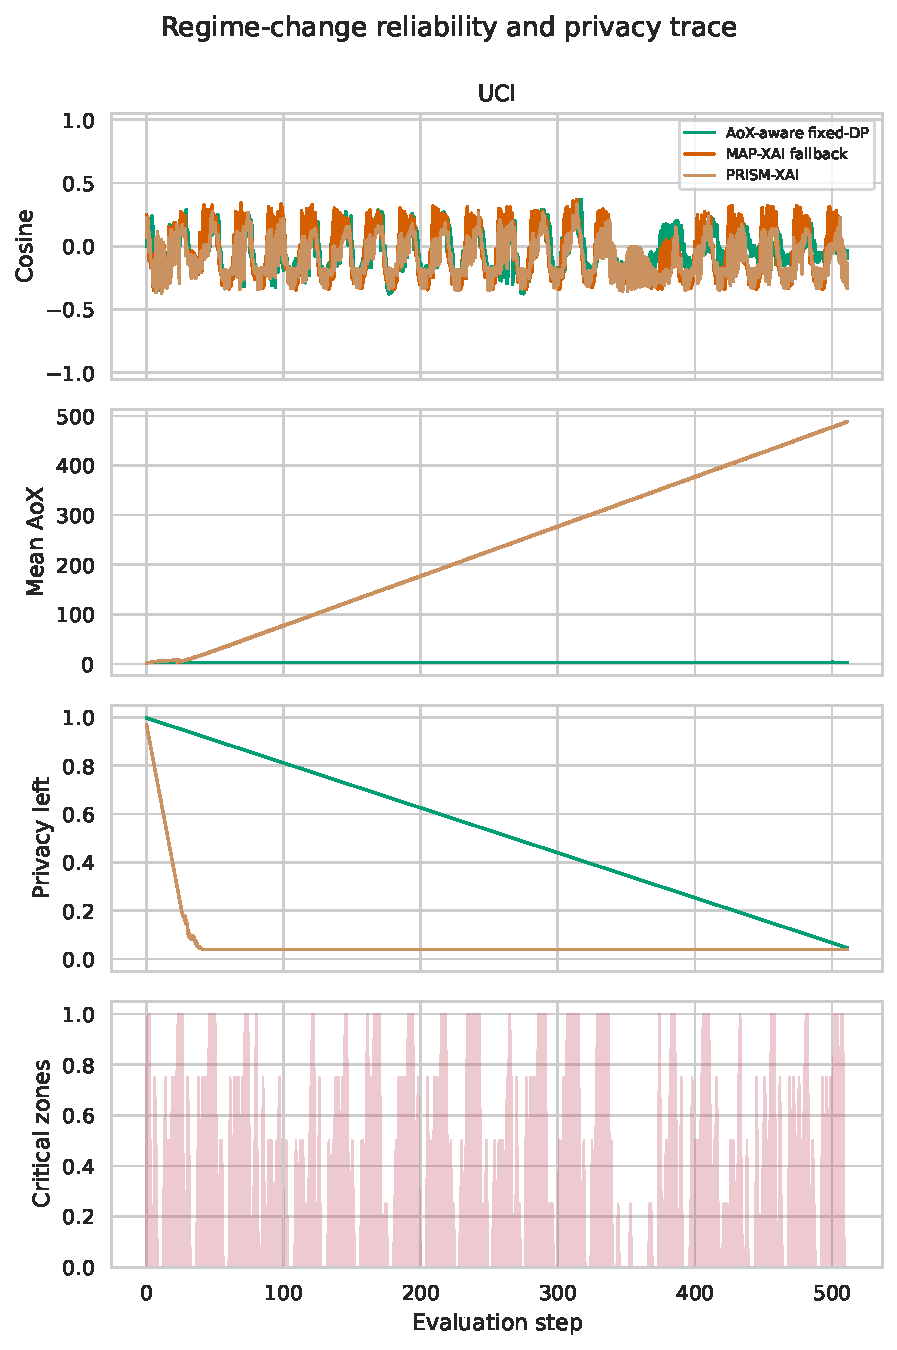
\includegraphics[width=.96\textwidth,height=.82\textheight,keepaspectratio]{../../SERVICE_TRADEOFF_RESULTS/runs/thr_0.5_cap_8/uci/regime_trace.pdf}

\caption{Public-score threshold $\tau=0.5$, release cap $M=8$, UCI: representative regime trace. This panel should be read with the setting-level quantitative interpretation and the complete tables immediately preceding the figure block.}

\end{figure*}

\clearpage

\begin{figure*}[p]

\centering

\includegraphics[width=.96\textwidth,height=.82\textheight,keepaspectratio]{../../SERVICE_TRADEOFF_RESULTS/runs/thr_0.5_cap_8/uci/fairness_reliability.pdf}

\caption{Public-score threshold $\tau=0.5$, release cap $M=8$, UCI: fairness--reliability plane. This panel should be read with the setting-level quantitative interpretation and the complete tables immediately preceding the figure block.}

\end{figure*}

\clearpage

\begin{figure*}[p]

\centering

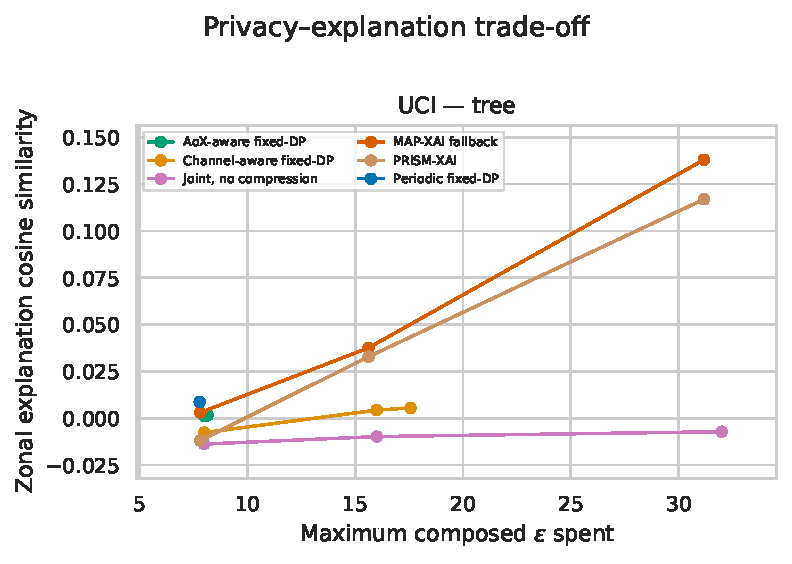
\includegraphics[width=.96\textwidth,height=.82\textheight,keepaspectratio]{../../SERVICE_TRADEOFF_RESULTS/runs/thr_0.5_cap_8/uci/privacy_fidelity.pdf}

\caption{Public-score threshold $\tau=0.5$, release cap $M=8$, UCI: privacy--fidelity plane. This panel should be read with the setting-level quantitative interpretation and the complete tables immediately preceding the figure block.}

\end{figure*}

\clearpage

\begin{figure*}[p]

\centering

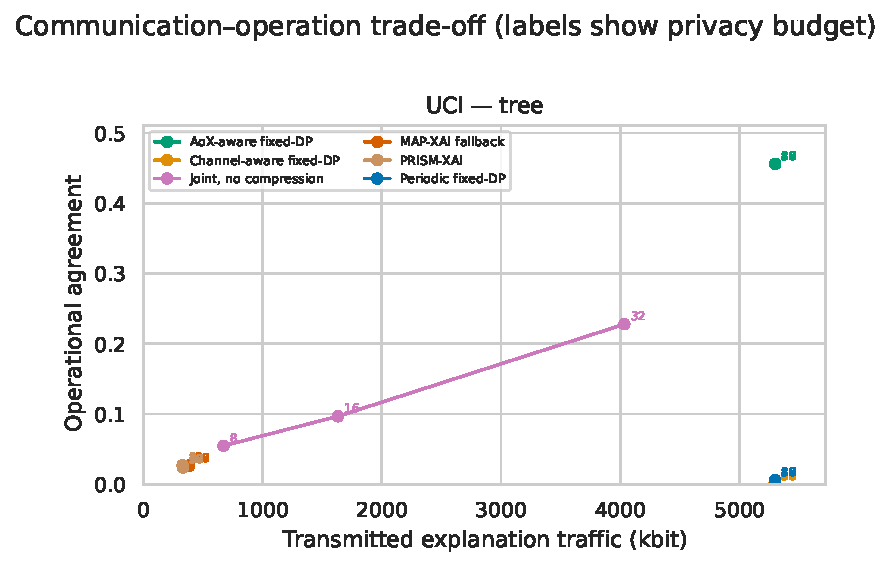
\includegraphics[width=.96\textwidth,height=.82\textheight,keepaspectratio]{../../SERVICE_TRADEOFF_RESULTS/runs/thr_0.5_cap_8/uci/pareto_bits_fidelity.pdf}

\caption{Public-score threshold $\tau=0.5$, release cap $M=8$, UCI: traffic--fidelity Pareto plane. This panel should be read with the setting-level quantitative interpretation and the complete tables immediately preceding the figure block.}

\end{figure*}

\clearpage

\begin{figure*}[p]

\centering

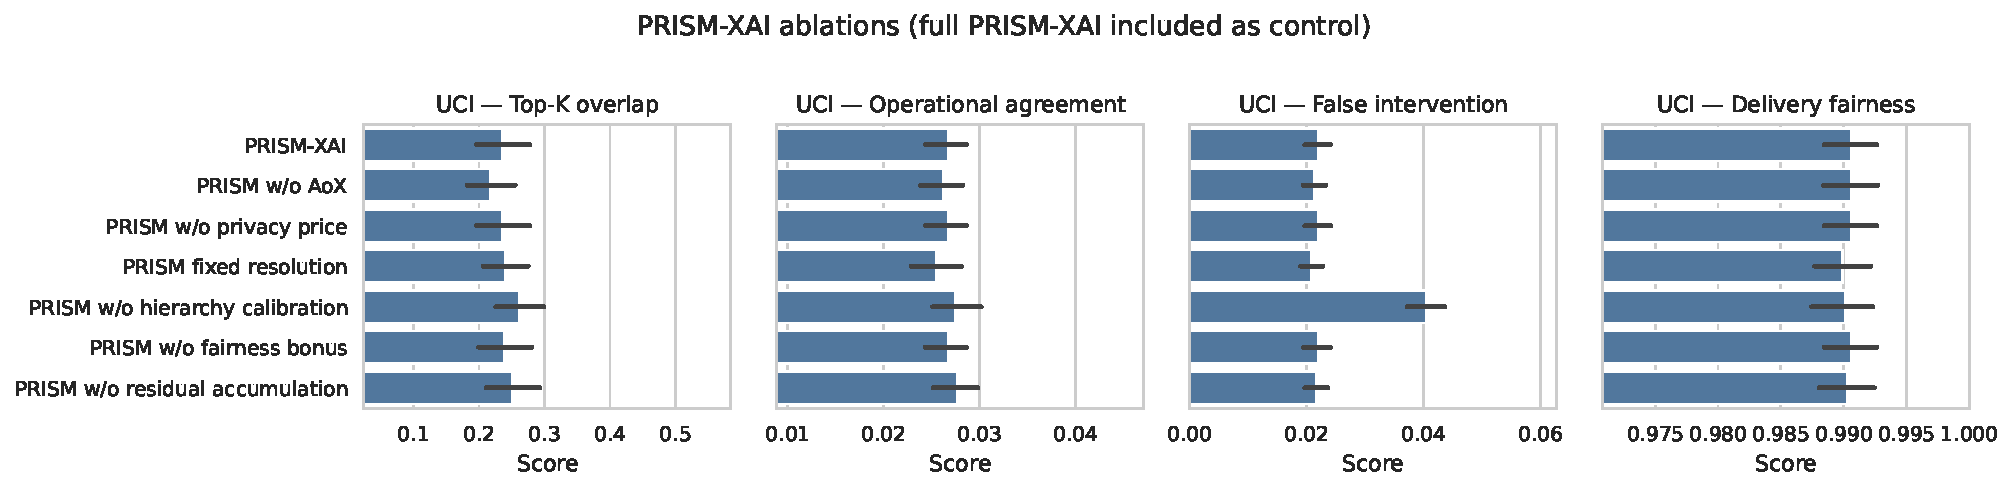
\includegraphics[width=.96\textwidth,height=.82\textheight,keepaspectratio]{../../SERVICE_TRADEOFF_RESULTS/runs/thr_0.5_cap_8/uci/ablation_results.pdf}

\caption{Public-score threshold $\tau=0.5$, release cap $M=8$, UCI: component ablation. This panel should be read with the setting-level quantitative interpretation and the complete tables immediately preceding the figure block.}

\end{figure*}

\clearpage

\subsubsection{Public-score threshold $\tau=1$, release cap $M=8$}

At this operating point, PRISM-XAI transmits 206.42~kbit versus 243.80~kbit for MAP-XAI-only (aggregate-mean ratio saving 15.33\%). The paired difference is -37.38$\pm$3.49~kbit. PRISM coverage is 0.0510, critical-event recall is 0.0230, and maximum recorded expenditure is 18.206. Relative to MAP-XAI-only, the paired coverage change is -0.00082$\pm$0.00060 and recall change is -0.00086$\pm$0.00107. The descriptive overlap rule holds in 12 of 12 cells. Accordingly, this point is read as a matched-service scheduler comparison.

\paragraph{Combined datasets.} The three generated tables below report the full method means, all condition-level values, and paired differences. The five figures that follow provide the corresponding temporal, fairness, privacy, Pareto, and ablation views. Aggregate panels support the setting-level summary above; dataset panels reveal whether that summary is shared by OPSD and UCI rather than being driven by their different endpoint counts.

\begin{table*}[p]\centering\tiny

\caption{Public-score threshold $\tau=1$, release cap $M=8$, Combined datasets: complete generated method table.}

\label{tab:thr_1_cap_8:combined:main}

\resizebox{\linewidth}{!}{% Values are means with 95% Student-t confidence intervals across seeds.
\begin{tabular}{lccccccccccccccc}
\toprule
Dataset & Model & $\epsilon_{\max}$ & Method & Top-$K$ & Cosine & Decision & Recall & Prec. & Abst. & P95 ms & kbit & Spent $\epsilon$ & False int. & bit/correct & Fairness \\
\midrule
OPSD & Tree & 8 & AoX-aware fixed-DP & 0.234 $\pm$ 0.048 & -0.033 $\pm$ 0.028 & 0.119 $\pm$ 0.028 & 0.119 $\pm$ 0.028 & 0.198 $\pm$ 0.054 & 0.721 $\pm$ 0.005 & 6.903 $\pm$ 1.126 & 1560.564 $\pm$ 0.000 & 7.990 $\pm$ 0.000 & 0.183 $\pm$ 0.020 & 35567.482 $\pm$ 10569.818 & 0.999 $\pm$ 0.000 \\
OPSD & Tree & 8 & AoX-aware fixed-DP & 0.238 $\pm$ 0.049 & -0.026 $\pm$ 0.055 & 0.121 $\pm$ 0.026 & 0.121 $\pm$ 0.026 & 0.205 $\pm$ 0.053 & 0.721 $\pm$ 0.005 & 6.903 $\pm$ 1.126 & 1560.564 $\pm$ 0.000 & 7.990 $\pm$ 0.000 & 0.179 $\pm$ 0.023 & 34123.214 $\pm$ 8376.542 & 0.999 $\pm$ 0.000 \\
OPSD & Tree & 8 & Channel-aware fixed-DP & 0.292 $\pm$ 0.037 & -0.041 $\pm$ 0.051 & 0.107 $\pm$ 0.026 & 0.107 $\pm$ 0.026 & 0.217 $\pm$ 0.068 & 0.779 $\pm$ 0.011 & 5.571 $\pm$ 1.784 & 1560.564 $\pm$ 0.000 & 7.990 $\pm$ 0.000 & 0.154 $\pm$ 0.029 & 40860.756 $\pm$ 14126.920 & 0.999 $\pm$ 0.000 \\
OPSD & Tree & 8 & Channel-aware fixed-DP & 0.292 $\pm$ 0.054 & -0.049 $\pm$ 0.064 & 0.111 $\pm$ 0.023 & 0.111 $\pm$ 0.023 & 0.228 $\pm$ 0.066 & 0.779 $\pm$ 0.011 & 5.571 $\pm$ 1.784 & 1560.564 $\pm$ 0.000 & 7.990 $\pm$ 0.000 & 0.149 $\pm$ 0.026 & 37980.855 $\pm$ 12338.094 & 0.999 $\pm$ 0.000 \\
OPSD & Tree & 8 & Joint, no compression & 0.288 $\pm$ 0.064 & -0.030 $\pm$ 0.079 & 0.016 $\pm$ 0.005 & 0.016 $\pm$ 0.005 & 0.193 $\pm$ 0.059 & 0.957 $\pm$ 0.003 & 4.560 $\pm$ 1.811 & 189.900 $\pm$ 0.554 & 7.990 $\pm$ 0.000 & 0.027 $\pm$ 0.005 & 32490.357 $\pm$ 10149.755 & 0.996 $\pm$ 0.002 \\
OPSD & Tree & 8 & Joint, no compression & 0.258 $\pm$ 0.055 & 0.011 $\pm$ 0.094 & 0.019 $\pm$ 0.004 & 0.019 $\pm$ 0.004 & 0.224 $\pm$ 0.044 & 0.957 $\pm$ 0.003 & 4.562 $\pm$ 1.809 & 189.750 $\pm$ 0.566 & 7.990 $\pm$ 0.000 & 0.025 $\pm$ 0.003 & 26079.167 $\pm$ 6335.386 & 0.996 $\pm$ 0.002 \\
OPSD & Tree & 8 & Periodic fixed-DP & 0.241 $\pm$ 0.049 & -0.019 $\pm$ 0.061 & 0.125 $\pm$ 0.020 & 0.125 $\pm$ 0.020 & 0.209 $\pm$ 0.044 & 0.722 $\pm$ 0.006 & 6.303 $\pm$ 1.438 & 1560.564 $\pm$ 0.000 & 7.990 $\pm$ 0.000 & 0.181 $\pm$ 0.021 & 31183.082 $\pm$ 4356.378 & 0.999 $\pm$ 0.000 \\
OPSD & Tree & 8 & Periodic fixed-DP & 0.242 $\pm$ 0.048 & -0.026 $\pm$ 0.082 & 0.135 $\pm$ 0.016 & 0.135 $\pm$ 0.016 & 0.231 $\pm$ 0.037 & 0.722 $\pm$ 0.006 & 6.303 $\pm$ 1.438 & 1560.564 $\pm$ 0.000 & 7.990 $\pm$ 0.000 & 0.169 $\pm$ 0.017 & 28520.235 $\pm$ 3511.595 & 0.999 $\pm$ 0.000 \\
OPSD & Tree & 8 & PRISM-XAI & 0.271 $\pm$ 0.064 & -0.008 $\pm$ 0.077 & 0.018 $\pm$ 0.004 & 0.018 $\pm$ 0.004 & 0.219 $\pm$ 0.073 & 0.956 $\pm$ 0.003 & 4.630 $\pm$ 1.839 & 87.543 $\pm$ 0.387 & 7.823 $\pm$ 0.000 & 0.026 $\pm$ 0.006 & 12978.492 $\pm$ 2874.959 & 0.993 $\pm$ 0.004 \\
OPSD & Tree & 8 & PRISM-XAI & 0.269 $\pm$ 0.071 & 0.002 $\pm$ 0.071 & 0.017 $\pm$ 0.005 & 0.017 $\pm$ 0.005 & 0.217 $\pm$ 0.065 & 0.956 $\pm$ 0.003 & 4.622 $\pm$ 1.845 & 87.369 $\pm$ 0.346 & 7.823 $\pm$ 0.000 & 0.024 $\pm$ 0.005 & 13859.274 $\pm$ 3369.246 & 0.994 $\pm$ 0.004 \\
OPSD & Tree & 8 & MAP-XAI fallback & 0.225 $\pm$ 0.063 & -0.029 $\pm$ 0.071 & 0.015 $\pm$ 0.006 & 0.015 $\pm$ 0.006 & 0.190 $\pm$ 0.076 & 0.956 $\pm$ 0.003 & 4.732 $\pm$ 1.776 & 105.817 $\pm$ 0.049 & 7.823 $\pm$ 0.000 & 0.026 $\pm$ 0.006 & 22620.844 $\pm$ 10124.929 & 0.993 $\pm$ 0.004 \\
OPSD & Tree & 8 & MAP-XAI fallback & 0.251 $\pm$ 0.064 & -0.005 $\pm$ 0.077 & 0.017 $\pm$ 0.006 & 0.017 $\pm$ 0.006 & 0.217 $\pm$ 0.076 & 0.956 $\pm$ 0.003 & 4.732 $\pm$ 1.776 & 105.675 $\pm$ 0.049 & 7.823 $\pm$ 0.000 & 0.024 $\pm$ 0.006 & 18265.481 $\pm$ 6339.471 & 0.993 $\pm$ 0.004 \\
UCI & Tree & 8 & AoX-aware fixed-DP & 0.263 $\pm$ 0.041 & -0.007 $\pm$ 0.009 & 0.457 $\pm$ 0.031 & 0.457 $\pm$ 0.031 & 0.362 $\pm$ 0.024 & 0.003 $\pm$ 0.001 & 7.500 $\pm$ 0.000 & 5300.224 $\pm$ 0.000 & 7.990 $\pm$ 0.000 & 0.557 $\pm$ 0.025 & 14002.896 $\pm$ 1040.243 & 0.999 $\pm$ 0.000 \\
UCI & Tree & 8 & AoX-aware fixed-DP & 0.260 $\pm$ 0.022 & 0.010 $\pm$ 0.055 & 0.455 $\pm$ 0.047 & 0.455 $\pm$ 0.047 & 0.361 $\pm$ 0.038 & 0.003 $\pm$ 0.001 & 7.500 $\pm$ 0.000 & 5300.224 $\pm$ 0.000 & 7.990 $\pm$ 0.000 & 0.557 $\pm$ 0.048 & 14198.303 $\pm$ 1508.274 & 0.999 $\pm$ 0.000 \\
UCI & Tree & 8 & Channel-aware fixed-DP & 0.248 $\pm$ 0.031 & 0.004 $\pm$ 0.012 & 0.001 $\pm$ 0.001 & 0.001 $\pm$ 0.001 & 0.150 $\pm$ 0.151 & 0.999 $\pm$ 0.001 & 4.609 $\pm$ 1.781 & 5295.177 $\pm$ 3.740 & 7.990 $\pm$ 0.000 & 0.001 $\pm$ 0.001 & 4632196.500 $\pm$ 2102650.252 & 0.991 $\pm$ 0.001 \\
UCI & Tree & 8 & Channel-aware fixed-DP & 0.239 $\pm$ 0.030 & -0.020 $\pm$ 0.055 & 0.000 $\pm$ 0.000 & 0.000 $\pm$ 0.000 & 0.117 $\pm$ 0.225 & 0.999 $\pm$ 0.001 & 4.609 $\pm$ 1.781 & 5295.177 $\pm$ 3.740 & 7.990 $\pm$ 0.000 & 0.001 $\pm$ 0.001 & 5296989.000 $\pm$ 41104.572 & 0.991 $\pm$ 0.001 \\
UCI & Tree & 8 & Joint, no compression & 0.286 $\pm$ 0.045 & 0.004 $\pm$ 0.020 & 0.052 $\pm$ 0.005 & 0.052 $\pm$ 0.005 & 0.406 $\pm$ 0.037 & 0.875 $\pm$ 0.003 & 5.123 $\pm$ 1.792 & 672.300 $\pm$ 0.452 & 7.990 $\pm$ 0.000 & 0.053 $\pm$ 0.004 & 15676.175 $\pm$ 1475.621 & 0.994 $\pm$ 0.003 \\
UCI & Tree & 8 & Joint, no compression & 0.229 $\pm$ 0.052 & -0.032 $\pm$ 0.050 & 0.057 $\pm$ 0.007 & 0.057 $\pm$ 0.007 & 0.428 $\pm$ 0.041 & 0.875 $\pm$ 0.003 & 5.131 $\pm$ 1.787 & 672.300 $\pm$ 0.452 & 7.990 $\pm$ 0.000 & 0.052 $\pm$ 0.004 & 14702.786 $\pm$ 2334.488 & 0.994 $\pm$ 0.003 \\
UCI & Tree & 8 & Periodic fixed-DP & 0.259 $\pm$ 0.060 & -0.005 $\pm$ 0.008 & 0.006 $\pm$ 0.001 & 0.006 $\pm$ 0.001 & 0.244 $\pm$ 0.049 & 0.989 $\pm$ 0.001 & 4.596 $\pm$ 1.788 & 5299.318 $\pm$ 1.451 & 7.786 $\pm$ 0.000 & 0.013 $\pm$ 0.002 & 1215103.896 $\pm$ 390671.319 & 0.999 $\pm$ 0.000 \\
UCI & Tree & 8 & Periodic fixed-DP & 0.260 $\pm$ 0.044 & 0.022 $\pm$ 0.070 & 0.005 $\pm$ 0.001 & 0.005 $\pm$ 0.001 & 0.195 $\pm$ 0.050 & 0.989 $\pm$ 0.001 & 4.596 $\pm$ 1.788 & 5299.318 $\pm$ 1.451 & 7.786 $\pm$ 0.000 & 0.015 $\pm$ 0.002 & 1555837.203 $\pm$ 955472.503 & 0.999 $\pm$ 0.000 \\
UCI & Tree & 8 & PRISM-XAI & 0.228 $\pm$ 0.051 & -0.001 $\pm$ 0.021 & 0.031 $\pm$ 0.005 & 0.031 $\pm$ 0.005 & 0.433 $\pm$ 0.052 & 0.933 $\pm$ 0.005 & 4.578 $\pm$ 1.800 & 323.463 $\pm$ 1.280 & 7.823 $\pm$ 0.000 & 0.029 $\pm$ 0.005 & 12910.343 $\pm$ 2005.939 & 0.992 $\pm$ 0.002 \\
UCI & Tree & 8 & PRISM-XAI & 0.219 $\pm$ 0.034 & -0.052 $\pm$ 0.048 & 0.025 $\pm$ 0.003 & 0.025 $\pm$ 0.003 & 0.390 $\pm$ 0.053 & 0.940 $\pm$ 0.005 & 4.798 $\pm$ 1.710 & 322.302 $\pm$ 1.580 & 7.823 $\pm$ 0.000 & 0.028 $\pm$ 0.004 & 15856.808 $\pm$ 2743.852 & 0.990 $\pm$ 0.005 \\
UCI & Tree & 8 & MAP-XAI fallback & 0.220 $\pm$ 0.055 & -0.006 $\pm$ 0.023 & 0.032 $\pm$ 0.005 & 0.032 $\pm$ 0.005 & 0.453 $\pm$ 0.058 & 0.932 $\pm$ 0.004 & 4.643 $\pm$ 1.763 & 382.099 $\pm$ 0.159 & 7.823 $\pm$ 0.000 & 0.027 $\pm$ 0.004 & 14883.660 $\pm$ 3313.232 & 0.992 $\pm$ 0.002 \\
UCI & Tree & 8 & MAP-XAI fallback & 0.250 $\pm$ 0.054 & 0.006 $\pm$ 0.060 & 0.030 $\pm$ 0.005 & 0.030 $\pm$ 0.005 & 0.453 $\pm$ 0.060 & 0.935 $\pm$ 0.006 & 5.564 $\pm$ 1.788 & 381.645 $\pm$ 0.090 & 7.823 $\pm$ 0.000 & 0.025 $\pm$ 0.004 & 15932.448 $\pm$ 2964.700 & 0.990 $\pm$ 0.005 \\
\bottomrule
\end{tabular}
}

\end{table*}\clearpage

\begin{table*}[p]\centering\tiny

\caption{Public-score threshold $\tau=1$, release cap $M=8$, Combined datasets: complete condition-level generated table.}

\label{tab:thr_1_cap_8:combined:conditions}

\resizebox{\textwidth}{!}{\begin{tabular}{llllccccccccccc}
\toprule
Dataset & Model & $\epsilon_{\max}$ & Method & kbit & Top-$K$ & Random Top-$K$ & Cosine & Decision & Recall & Precision & Coverage & Abstain & False int. & Spent $\epsilon$ \\
\midrule
OPSD & Tree & 8 & Joint, no compression & 189.900 $\pm$ 0.554 & 0.288 $\pm$ 0.064 & 0.250 $\pm$ 0.000 & -0.030 $\pm$ 0.079 & 0.016 $\pm$ 0.005 & 0.016 $\pm$ 0.005 & 0.193 $\pm$ 0.059 & 0.043 $\pm$ 0.003 & 0.957 $\pm$ 0.003 & 0.027 $\pm$ 0.005 & 7.990 $\pm$ 0.000 \\
OPSD & Tree & 8 & Joint, no compression & 189.750 $\pm$ 0.566 & 0.258 $\pm$ 0.055 & 0.250 $\pm$ 0.000 & 0.011 $\pm$ 0.094 & 0.019 $\pm$ 0.004 & 0.019 $\pm$ 0.004 & 0.224 $\pm$ 0.044 & 0.043 $\pm$ 0.003 & 0.957 $\pm$ 0.003 & 0.025 $\pm$ 0.003 & 7.990 $\pm$ 0.000 \\
OPSD & Tree & 8 & Periodic fixed-DP & 1560.564 $\pm$ 0.000 & 0.241 $\pm$ 0.049 & 0.250 $\pm$ 0.000 & -0.019 $\pm$ 0.061 & 0.125 $\pm$ 0.020 & 0.125 $\pm$ 0.020 & 0.209 $\pm$ 0.044 & 0.278 $\pm$ 0.006 & 0.722 $\pm$ 0.006 & 0.181 $\pm$ 0.021 & 7.990 $\pm$ 0.000 \\
OPSD & Tree & 8 & Periodic fixed-DP & 1560.564 $\pm$ 0.000 & 0.242 $\pm$ 0.048 & 0.250 $\pm$ 0.000 & -0.026 $\pm$ 0.082 & 0.135 $\pm$ 0.016 & 0.135 $\pm$ 0.016 & 0.231 $\pm$ 0.037 & 0.278 $\pm$ 0.006 & 0.722 $\pm$ 0.006 & 0.169 $\pm$ 0.017 & 7.990 $\pm$ 0.000 \\
OPSD & Tree & 8 & PRISM-XAI & 87.543 $\pm$ 0.387 & 0.271 $\pm$ 0.064 & 0.250 $\pm$ 0.000 & -0.008 $\pm$ 0.077 & 0.018 $\pm$ 0.004 & 0.018 $\pm$ 0.004 & 0.219 $\pm$ 0.073 & 0.044 $\pm$ 0.003 & 0.956 $\pm$ 0.003 & 0.026 $\pm$ 0.006 & 7.823 $\pm$ 0.000 \\
OPSD & Tree & 8 & PRISM-XAI & 87.369 $\pm$ 0.346 & 0.269 $\pm$ 0.071 & 0.250 $\pm$ 0.000 & 0.002 $\pm$ 0.071 & 0.017 $\pm$ 0.005 & 0.017 $\pm$ 0.005 & 0.217 $\pm$ 0.065 & 0.044 $\pm$ 0.003 & 0.956 $\pm$ 0.003 & 0.024 $\pm$ 0.005 & 7.823 $\pm$ 0.000 \\
OPSD & Tree & 16 & Joint, no compression & 459.900 $\pm$ 0.750 & 0.232 $\pm$ 0.065 & 0.250 $\pm$ 0.000 & 0.059 $\pm$ 0.048 & 0.038 $\pm$ 0.009 & 0.038 $\pm$ 0.009 & 0.222 $\pm$ 0.049 & 0.088 $\pm$ 0.004 & 0.912 $\pm$ 0.004 & 0.049 $\pm$ 0.005 & 15.997 $\pm$ 0.000 \\
OPSD & Tree & 16 & Joint, no compression & 460.050 $\pm$ 0.724 & 0.241 $\pm$ 0.055 & 0.250 $\pm$ 0.000 & 0.061 $\pm$ 0.052 & 0.039 $\pm$ 0.008 & 0.039 $\pm$ 0.008 & 0.241 $\pm$ 0.042 & 0.088 $\pm$ 0.004 & 0.912 $\pm$ 0.004 & 0.045 $\pm$ 0.004 & 15.997 $\pm$ 0.000 \\
OPSD & Tree & 16 & Periodic fixed-DP & 5112.594 $\pm$ 0.000 & 0.249 $\pm$ 0.022 & 0.250 $\pm$ 0.000 & -0.009 $\pm$ 0.045 & 0.450 $\pm$ 0.062 & 0.450 $\pm$ 0.062 & 0.237 $\pm$ 0.042 & 0.985 $\pm$ 0.002 & 0.015 $\pm$ 0.002 & 0.551 $\pm$ 0.057 & 15.997 $\pm$ 0.000 \\
OPSD & Tree & 16 & Periodic fixed-DP & 5112.594 $\pm$ 0.000 & 0.243 $\pm$ 0.019 & 0.250 $\pm$ 0.000 & -0.012 $\pm$ 0.050 & 0.463 $\pm$ 0.047 & 0.463 $\pm$ 0.047 & 0.240 $\pm$ 0.028 & 0.985 $\pm$ 0.002 & 0.015 $\pm$ 0.002 & 0.547 $\pm$ 0.036 & 15.997 $\pm$ 0.000 \\
OPSD & Tree & 16 & PRISM-XAI & 87.513 $\pm$ 0.398 & 0.282 $\pm$ 0.051 & 0.250 $\pm$ 0.000 & 0.088 $\pm$ 0.071 & 0.018 $\pm$ 0.005 & 0.018 $\pm$ 0.005 & 0.230 $\pm$ 0.080 & 0.044 $\pm$ 0.003 & 0.956 $\pm$ 0.003 & 0.024 $\pm$ 0.006 & 15.620 $\pm$ 0.000 \\
OPSD & Tree & 16 & PRISM-XAI & 87.369 $\pm$ 0.313 & 0.275 $\pm$ 0.076 & 0.250 $\pm$ 0.000 & 0.136 $\pm$ 0.053 & 0.018 $\pm$ 0.006 & 0.018 $\pm$ 0.006 & 0.236 $\pm$ 0.080 & 0.044 $\pm$ 0.003 & 0.956 $\pm$ 0.003 & 0.024 $\pm$ 0.006 & 15.620 $\pm$ 0.000 \\
OPSD & Tree & 32 & Joint, no compression & 1140.900 $\pm$ 7.953 & 0.235 $\pm$ 0.064 & 0.250 $\pm$ 0.000 & -0.031 $\pm$ 0.089 & 0.074 $\pm$ 0.015 & 0.074 $\pm$ 0.015 & 0.205 $\pm$ 0.039 & 0.157 $\pm$ 0.006 & 0.843 $\pm$ 0.006 & 0.107 $\pm$ 0.009 & 31.999 $\pm$ 0.000 \\
OPSD & Tree & 32 & Joint, no compression & 1140.900 $\pm$ 7.953 & 0.282 $\pm$ 0.054 & 0.250 $\pm$ 0.000 & -0.044 $\pm$ 0.076 & 0.080 $\pm$ 0.011 & 0.080 $\pm$ 0.011 & 0.227 $\pm$ 0.052 & 0.158 $\pm$ 0.006 & 0.842 $\pm$ 0.006 & 0.105 $\pm$ 0.015 & 31.999 $\pm$ 0.000 \\
OPSD & Tree & 32 & Periodic fixed-DP & 5299.836 $\pm$ 0.625 & 0.249 $\pm$ 0.022 & 0.250 $\pm$ 0.000 & -0.009 $\pm$ 0.044 & 0.458 $\pm$ 0.066 & 0.458 $\pm$ 0.066 & 0.237 $\pm$ 0.045 & 1.000 $\pm$ 0.000 & 0.000 $\pm$ 0.000 & 0.562 $\pm$ 0.062 & 16.371 $\pm$ 0.000 \\
OPSD & Tree & 32 & Periodic fixed-DP & 5299.836 $\pm$ 0.625 & 0.244 $\pm$ 0.019 & 0.250 $\pm$ 0.000 & -0.012 $\pm$ 0.050 & 0.471 $\pm$ 0.049 & 0.471 $\pm$ 0.049 & 0.240 $\pm$ 0.029 & 1.000 $\pm$ 0.000 & 0.000 $\pm$ 0.000 & 0.559 $\pm$ 0.039 & 16.371 $\pm$ 0.000 \\
OPSD & Tree & 32 & PRISM-XAI & 87.482 $\pm$ 0.366 & 0.365 $\pm$ 0.069 & 0.250 $\pm$ 0.000 & 0.225 $\pm$ 0.051 & 0.022 $\pm$ 0.005 & 0.022 $\pm$ 0.005 & 0.373 $\pm$ 0.132 & 0.044 $\pm$ 0.003 & 0.956 $\pm$ 0.003 & 0.015 $\pm$ 0.005 & 31.175 $\pm$ 0.000 \\
OPSD & Tree & 32 & PRISM-XAI & 87.185 $\pm$ 0.219 & 0.398 $\pm$ 0.060 & 0.250 $\pm$ 0.000 & 0.291 $\pm$ 0.044 & 0.022 $\pm$ 0.005 & 0.022 $\pm$ 0.005 & 0.365 $\pm$ 0.152 & 0.044 $\pm$ 0.003 & 0.956 $\pm$ 0.003 & 0.017 $\pm$ 0.006 & 31.175 $\pm$ 0.000 \\
UCI & Tree & 8 & Joint, no compression & 672.300 $\pm$ 0.452 & 0.286 $\pm$ 0.045 & 0.250 $\pm$ 0.000 & 0.004 $\pm$ 0.020 & 0.052 $\pm$ 0.005 & 0.052 $\pm$ 0.005 & 0.406 $\pm$ 0.037 & 0.125 $\pm$ 0.003 & 0.875 $\pm$ 0.003 & 0.053 $\pm$ 0.004 & 7.990 $\pm$ 0.000 \\
UCI & Tree & 8 & Joint, no compression & 672.300 $\pm$ 0.452 & 0.229 $\pm$ 0.052 & 0.250 $\pm$ 0.000 & -0.032 $\pm$ 0.050 & 0.057 $\pm$ 0.007 & 0.057 $\pm$ 0.007 & 0.428 $\pm$ 0.041 & 0.125 $\pm$ 0.003 & 0.875 $\pm$ 0.003 & 0.052 $\pm$ 0.004 & 7.990 $\pm$ 0.000 \\
UCI & Tree & 8 & Periodic fixed-DP & 5299.318 $\pm$ 1.451 & 0.259 $\pm$ 0.060 & 0.250 $\pm$ 0.000 & -0.005 $\pm$ 0.008 & 0.006 $\pm$ 0.001 & 0.006 $\pm$ 0.001 & 0.244 $\pm$ 0.049 & 0.011 $\pm$ 0.001 & 0.989 $\pm$ 0.001 & 0.013 $\pm$ 0.002 & 7.786 $\pm$ 0.000 \\
UCI & Tree & 8 & Periodic fixed-DP & 5299.318 $\pm$ 1.451 & 0.260 $\pm$ 0.044 & 0.250 $\pm$ 0.000 & 0.022 $\pm$ 0.070 & 0.005 $\pm$ 0.001 & 0.005 $\pm$ 0.001 & 0.195 $\pm$ 0.050 & 0.011 $\pm$ 0.001 & 0.989 $\pm$ 0.001 & 0.015 $\pm$ 0.002 & 7.786 $\pm$ 0.000 \\
UCI & Tree & 8 & PRISM-XAI & 323.463 $\pm$ 1.280 & 0.228 $\pm$ 0.051 & 0.250 $\pm$ 0.000 & -0.001 $\pm$ 0.021 & 0.031 $\pm$ 0.005 & 0.031 $\pm$ 0.005 & 0.433 $\pm$ 0.052 & 0.067 $\pm$ 0.005 & 0.933 $\pm$ 0.005 & 0.029 $\pm$ 0.005 & 7.823 $\pm$ 0.000 \\
UCI & Tree & 8 & PRISM-XAI & 322.302 $\pm$ 1.580 & 0.219 $\pm$ 0.034 & 0.250 $\pm$ 0.000 & -0.052 $\pm$ 0.048 & 0.025 $\pm$ 0.003 & 0.025 $\pm$ 0.003 & 0.390 $\pm$ 0.053 & 0.060 $\pm$ 0.005 & 0.940 $\pm$ 0.005 & 0.028 $\pm$ 0.004 & 7.823 $\pm$ 0.000 \\
UCI & Tree & 16 & Joint, no compression & 1632.150 $\pm$ 0.339 & 0.216 $\pm$ 0.041 & 0.250 $\pm$ 0.000 & 0.001 $\pm$ 0.012 & 0.094 $\pm$ 0.005 & 0.094 $\pm$ 0.005 & 0.330 $\pm$ 0.024 & 0.228 $\pm$ 0.005 & 0.772 $\pm$ 0.005 & 0.133 $\pm$ 0.010 & 15.997 $\pm$ 0.000 \\
UCI & Tree & 16 & Joint, no compression & 1632.600 $\pm$ 0.554 & 0.204 $\pm$ 0.011 & 0.250 $\pm$ 0.000 & -0.021 $\pm$ 0.033 & 0.099 $\pm$ 0.016 & 0.099 $\pm$ 0.016 & 0.347 $\pm$ 0.054 & 0.228 $\pm$ 0.005 & 0.772 $\pm$ 0.005 & 0.128 $\pm$ 0.011 & 15.997 $\pm$ 0.000 \\
UCI & Tree & 16 & Periodic fixed-DP & 5299.318 $\pm$ 1.451 & 0.259 $\pm$ 0.060 & 0.250 $\pm$ 0.000 & -0.005 $\pm$ 0.008 & 0.006 $\pm$ 0.001 & 0.006 $\pm$ 0.001 & 0.244 $\pm$ 0.049 & 0.011 $\pm$ 0.001 & 0.989 $\pm$ 0.001 & 0.013 $\pm$ 0.002 & 7.786 $\pm$ 0.000 \\
UCI & Tree & 16 & Periodic fixed-DP & 5299.318 $\pm$ 1.451 & 0.260 $\pm$ 0.044 & 0.250 $\pm$ 0.000 & 0.022 $\pm$ 0.070 & 0.005 $\pm$ 0.001 & 0.005 $\pm$ 0.001 & 0.195 $\pm$ 0.050 & 0.011 $\pm$ 0.001 & 0.989 $\pm$ 0.001 & 0.015 $\pm$ 0.002 & 7.786 $\pm$ 0.000 \\
UCI & Tree & 16 & PRISM-XAI & 323.309 $\pm$ 1.557 & 0.217 $\pm$ 0.067 & 0.250 $\pm$ 0.000 & 0.003 $\pm$ 0.026 & 0.032 $\pm$ 0.005 & 0.032 $\pm$ 0.005 & 0.526 $\pm$ 0.039 & 0.066 $\pm$ 0.005 & 0.934 $\pm$ 0.005 & 0.020 $\pm$ 0.005 & 15.620 $\pm$ 0.000 \\
UCI & Tree & 16 & PRISM-XAI & 326.600 $\pm$ 1.887 & 0.258 $\pm$ 0.051 & 0.250 $\pm$ 0.000 & 0.042 $\pm$ 0.057 & 0.024 $\pm$ 0.003 & 0.024 $\pm$ 0.003 & 0.530 $\pm$ 0.088 & 0.051 $\pm$ 0.004 & 0.949 $\pm$ 0.004 & 0.016 $\pm$ 0.005 & 15.620 $\pm$ 0.000 \\
UCI & Tree & 32 & Joint, no compression & 4034.550 $\pm$ 5.034 & 0.246 $\pm$ 0.031 & 0.250 $\pm$ 0.000 & -0.002 $\pm$ 0.015 & 0.228 $\pm$ 0.013 & 0.228 $\pm$ 0.013 & 0.361 $\pm$ 0.028 & 0.537 $\pm$ 0.009 & 0.463 $\pm$ 0.009 & 0.279 $\pm$ 0.017 & 31.999 $\pm$ 0.000 \\
UCI & Tree & 32 & Joint, no compression & 4034.550 $\pm$ 5.034 & 0.241 $\pm$ 0.033 & 0.250 $\pm$ 0.000 & -0.012 $\pm$ 0.030 & 0.228 $\pm$ 0.028 & 0.228 $\pm$ 0.028 & 0.360 $\pm$ 0.047 & 0.530 $\pm$ 0.010 & 0.470 $\pm$ 0.010 & 0.280 $\pm$ 0.026 & 31.999 $\pm$ 0.000 \\
UCI & Tree & 32 & Periodic fixed-DP & 5299.318 $\pm$ 1.451 & 0.259 $\pm$ 0.060 & 0.250 $\pm$ 0.000 & -0.005 $\pm$ 0.008 & 0.006 $\pm$ 0.001 & 0.006 $\pm$ 0.001 & 0.244 $\pm$ 0.049 & 0.011 $\pm$ 0.001 & 0.989 $\pm$ 0.001 & 0.013 $\pm$ 0.002 & 7.786 $\pm$ 0.000 \\
UCI & Tree & 32 & Periodic fixed-DP & 5299.318 $\pm$ 1.451 & 0.260 $\pm$ 0.044 & 0.250 $\pm$ 0.000 & 0.022 $\pm$ 0.070 & 0.005 $\pm$ 0.001 & 0.005 $\pm$ 0.001 & 0.195 $\pm$ 0.050 & 0.011 $\pm$ 0.001 & 0.989 $\pm$ 0.001 & 0.015 $\pm$ 0.002 & 7.786 $\pm$ 0.000 \\
UCI & Tree & 32 & PRISM-XAI & 328.006 $\pm$ 2.663 & 0.282 $\pm$ 0.083 & 0.250 $\pm$ 0.000 & 0.020 $\pm$ 0.013 & 0.026 $\pm$ 0.005 & 0.026 $\pm$ 0.005 & 0.974 $\pm$ 0.028 & 0.057 $\pm$ 0.006 & 0.943 $\pm$ 0.006 & 0.000 $\pm$ 0.001 & 31.175 $\pm$ 0.000 \\
UCI & Tree & 32 & PRISM-XAI & 328.933 $\pm$ 1.490 & 0.315 $\pm$ 0.048 & 0.250 $\pm$ 0.000 & 0.135 $\pm$ 0.042 & 0.023 $\pm$ 0.002 & 0.023 $\pm$ 0.002 & 0.909 $\pm$ 0.094 & 0.047 $\pm$ 0.002 & 0.953 $\pm$ 0.002 & 0.002 $\pm$ 0.002 & 31.175 $\pm$ 0.000 \\
\bottomrule
\end{tabular}
}

\end{table*}\clearpage

\begin{table*}[p]\centering\tiny

\caption{Public-score threshold $\tau=1$, release cap $M=8$, Combined datasets: complete generated paired comparisons.}

\label{tab:thr_1_cap_8:combined:paired}

\resizebox{\textwidth}{!}{\begin{tabular}{llcccc}
\toprule
Dataset & Baseline & Delta kbit & Delta Top-$K$ & Delta recall & Delta fairness \\
\midrule
OPSD & AoX-aware fixed-DP & -1473.021 $\pm$ 0.387 & 0.037 $\pm$ 0.076 & -0.102 $\pm$ 0.029 & -0.006 $\pm$ 0.004 \\
OPSD & AoX-aware fixed-DP & -5012.400 $\pm$ 5.552 & 0.029 $\pm$ 0.064 & -0.383 $\pm$ 0.074 & -0.006 $\pm$ 0.004 \\
OPSD & AoX-aware fixed-DP & -5212.742 $\pm$ 0.366 & 0.112 $\pm$ 0.088 & -0.391 $\pm$ 0.079 & -0.006 $\pm$ 0.005 \\
OPSD & AoX-aware fixed-DP & -1473.195 $\pm$ 0.346 & 0.030 $\pm$ 0.077 & -0.104 $\pm$ 0.026 & -0.006 $\pm$ 0.004 \\
OPSD & AoX-aware fixed-DP & -5012.544 $\pm$ 5.514 & 0.023 $\pm$ 0.077 & -0.396 $\pm$ 0.057 & -0.006 $\pm$ 0.004 \\
OPSD & AoX-aware fixed-DP & -5213.039 $\pm$ 0.219 & 0.147 $\pm$ 0.078 & -0.403 $\pm$ 0.059 & -0.006 $\pm$ 0.005 \\
OPSD & Channel-aware fixed-DP & -1473.021 $\pm$ 0.387 & -0.021 $\pm$ 0.081 & -0.089 $\pm$ 0.026 & -0.006 $\pm$ 0.004 \\
OPSD & Channel-aware fixed-DP & -4599.097 $\pm$ 12.954 & 0.021 $\pm$ 0.063 & -0.383 $\pm$ 0.090 & 0.056 $\pm$ 0.006 \\
OPSD & Channel-aware fixed-DP & -5212.742 $\pm$ 0.366 & 0.107 $\pm$ 0.084 & -0.413 $\pm$ 0.099 & 0.087 $\pm$ 0.007 \\
OPSD & Channel-aware fixed-DP & -1473.195 $\pm$ 0.346 & -0.024 $\pm$ 0.075 & -0.094 $\pm$ 0.023 & -0.006 $\pm$ 0.004 \\
OPSD & Channel-aware fixed-DP & -4599.240 $\pm$ 12.910 & 0.017 $\pm$ 0.079 & -0.401 $\pm$ 0.088 & 0.056 $\pm$ 0.006 \\
OPSD & Channel-aware fixed-DP & -5213.039 $\pm$ 0.219 & 0.141 $\pm$ 0.071 & -0.434 $\pm$ 0.092 & 0.087 $\pm$ 0.007 \\
OPSD & Joint, no compression & -102.357 $\pm$ 0.507 & -0.017 $\pm$ 0.096 & 0.001 $\pm$ 0.004 & -0.002 $\pm$ 0.003 \\
OPSD & Joint, no compression & -372.387 $\pm$ 1.050 & 0.051 $\pm$ 0.071 & -0.020 $\pm$ 0.010 & -0.004 $\pm$ 0.004 \\
OPSD & Joint, no compression & -1053.418 $\pm$ 7.970 & 0.129 $\pm$ 0.123 & -0.052 $\pm$ 0.014 & -0.005 $\pm$ 0.005 \\
OPSD & Joint, no compression & -102.381 $\pm$ 0.421 & 0.010 $\pm$ 0.097 & -0.002 $\pm$ 0.003 & -0.002 $\pm$ 0.003 \\
OPSD & Joint, no compression & -372.681 $\pm$ 0.901 & 0.035 $\pm$ 0.072 & -0.020 $\pm$ 0.008 & -0.004 $\pm$ 0.004 \\
OPSD & Joint, no compression & -1053.715 $\pm$ 7.867 & 0.116 $\pm$ 0.104 & -0.058 $\pm$ 0.012 & -0.005 $\pm$ 0.005 \\
OPSD & Periodic fixed-DP & -1473.021 $\pm$ 0.387 & 0.031 $\pm$ 0.076 & -0.107 $\pm$ 0.021 & -0.006 $\pm$ 0.004 \\
OPSD & Periodic fixed-DP & -5025.081 $\pm$ 0.398 & 0.033 $\pm$ 0.059 & -0.432 $\pm$ 0.063 & -0.006 $\pm$ 0.004 \\
OPSD & Periodic fixed-DP & -5212.354 $\pm$ 0.641 & 0.116 $\pm$ 0.083 & -0.436 $\pm$ 0.068 & -0.007 $\pm$ 0.005 \\
OPSD & Periodic fixed-DP & -1473.195 $\pm$ 0.346 & 0.027 $\pm$ 0.083 & -0.118 $\pm$ 0.016 & -0.006 $\pm$ 0.004 \\
OPSD & Periodic fixed-DP & -5025.225 $\pm$ 0.313 & 0.032 $\pm$ 0.072 & -0.444 $\pm$ 0.049 & -0.006 $\pm$ 0.004 \\
OPSD & Periodic fixed-DP & -5212.651 $\pm$ 0.592 & 0.155 $\pm$ 0.065 & -0.449 $\pm$ 0.050 & -0.007 $\pm$ 0.005 \\
OPSD & MAP-XAI fallback & -18.273 $\pm$ 0.401 & 0.046 $\pm$ 0.070 & 0.002 $\pm$ 0.003 & 0.000 $\pm$ 0.000 \\
OPSD & MAP-XAI fallback & -18.304 $\pm$ 0.409 & 0.038 $\pm$ 0.045 & 0.001 $\pm$ 0.006 & 0.000 $\pm$ 0.000 \\
OPSD & MAP-XAI fallback & -18.335 $\pm$ 0.374 & 0.013 $\pm$ 0.060 & -0.002 $\pm$ 0.005 & -0.000 $\pm$ 0.001 \\
OPSD & MAP-XAI fallback & -18.306 $\pm$ 0.346 & 0.018 $\pm$ 0.054 & 0.000 $\pm$ 0.004 & 0.000 $\pm$ 0.000 \\
OPSD & MAP-XAI fallback & -18.285 $\pm$ 0.309 & 0.011 $\pm$ 0.065 & -0.000 $\pm$ 0.005 & 0.000 $\pm$ 0.000 \\
OPSD & MAP-XAI fallback & -18.367 $\pm$ 0.250 & 0.022 $\pm$ 0.068 & -0.002 $\pm$ 0.003 & -0.000 $\pm$ 0.000 \\
UCI & AoX-aware fixed-DP & -4976.761 $\pm$ 1.280 & -0.036 $\pm$ 0.068 & -0.426 $\pm$ 0.033 & -0.008 $\pm$ 0.002 \\
UCI & AoX-aware fixed-DP & -4976.915 $\pm$ 1.557 & -0.047 $\pm$ 0.088 & -0.425 $\pm$ 0.031 & -0.007 $\pm$ 0.003 \\
UCI & AoX-aware fixed-DP & -4972.218 $\pm$ 2.663 & 0.018 $\pm$ 0.072 & -0.431 $\pm$ 0.033 & -0.008 $\pm$ 0.004 \\
UCI & AoX-aware fixed-DP & -4977.922 $\pm$ 1.580 & -0.041 $\pm$ 0.037 & -0.430 $\pm$ 0.047 & -0.009 $\pm$ 0.005 \\
UCI & AoX-aware fixed-DP & -4973.624 $\pm$ 1.887 & -0.002 $\pm$ 0.064 & -0.430 $\pm$ 0.047 & -0.008 $\pm$ 0.002 \\
UCI & AoX-aware fixed-DP & -4971.291 $\pm$ 1.490 & 0.054 $\pm$ 0.058 & -0.431 $\pm$ 0.047 & -0.007 $\pm$ 0.002 \\
UCI & Channel-aware fixed-DP & -4971.715 $\pm$ 4.160 & -0.020 $\pm$ 0.068 & 0.031 $\pm$ 0.005 & 0.001 $\pm$ 0.002 \\
UCI & Channel-aware fixed-DP & -4976.915 $\pm$ 1.557 & -0.051 $\pm$ 0.075 & 0.031 $\pm$ 0.005 & 0.662 $\pm$ 0.003 \\
UCI & Channel-aware fixed-DP & -4972.218 $\pm$ 2.663 & 0.013 $\pm$ 0.098 & 0.025 $\pm$ 0.005 & 0.736 $\pm$ 0.004 \\
UCI & Channel-aware fixed-DP & -4972.875 $\pm$ 4.681 & -0.020 $\pm$ 0.051 & 0.025 $\pm$ 0.003 & -0.001 $\pm$ 0.005 \\
UCI & Channel-aware fixed-DP & -4973.624 $\pm$ 1.887 & -0.002 $\pm$ 0.063 & 0.024 $\pm$ 0.003 & 0.661 $\pm$ 0.002 \\
UCI & Channel-aware fixed-DP & -4971.291 $\pm$ 1.490 & 0.055 $\pm$ 0.057 & 0.023 $\pm$ 0.002 & 0.737 $\pm$ 0.003 \\
UCI & Joint, no compression & -348.837 $\pm$ 1.583 & -0.058 $\pm$ 0.074 & -0.021 $\pm$ 0.005 & -0.002 $\pm$ 0.004 \\
UCI & Joint, no compression & -1308.841 $\pm$ 1.426 & 0.000 $\pm$ 0.093 & -0.062 $\pm$ 0.006 & -0.005 $\pm$ 0.003 \\
UCI & Joint, no compression & -3706.543 $\pm$ 6.544 & 0.035 $\pm$ 0.097 & -0.202 $\pm$ 0.016 & -0.008 $\pm$ 0.004 \\
UCI & Joint, no compression & -349.998 $\pm$ 1.687 & -0.010 $\pm$ 0.045 & -0.031 $\pm$ 0.008 & -0.004 $\pm$ 0.005 \\
UCI & Joint, no compression & -1306.000 $\pm$ 2.008 & 0.054 $\pm$ 0.052 & -0.075 $\pm$ 0.017 & -0.006 $\pm$ 0.002 \\
UCI & Joint, no compression & -3705.617 $\pm$ 4.600 & 0.073 $\pm$ 0.055 & -0.204 $\pm$ 0.029 & -0.007 $\pm$ 0.002 \\
UCI & Periodic fixed-DP & -4975.855 $\pm$ 1.998 & -0.032 $\pm$ 0.088 & 0.025 $\pm$ 0.005 & -0.008 $\pm$ 0.002 \\
UCI & Periodic fixed-DP & -4976.009 $\pm$ 2.472 & -0.043 $\pm$ 0.092 & 0.026 $\pm$ 0.005 & -0.007 $\pm$ 0.003 \\
UCI & Periodic fixed-DP & -4971.312 $\pm$ 3.350 & 0.022 $\pm$ 0.066 & 0.020 $\pm$ 0.005 & -0.008 $\pm$ 0.004 \\
UCI & Periodic fixed-DP & -4977.016 $\pm$ 2.100 & -0.041 $\pm$ 0.062 & 0.020 $\pm$ 0.004 & -0.009 $\pm$ 0.005 \\
UCI & Periodic fixed-DP & -4972.718 $\pm$ 2.453 & -0.002 $\pm$ 0.064 & 0.019 $\pm$ 0.005 & -0.008 $\pm$ 0.002 \\
UCI & Periodic fixed-DP & -4970.385 $\pm$ 1.709 & 0.054 $\pm$ 0.055 & 0.018 $\pm$ 0.002 & -0.008 $\pm$ 0.002 \\
UCI & MAP-XAI fallback & -58.636 $\pm$ 1.168 & 0.008 $\pm$ 0.063 & -0.001 $\pm$ 0.003 & -0.000 $\pm$ 0.001 \\
UCI & MAP-XAI fallback & -58.851 $\pm$ 1.541 & 0.016 $\pm$ 0.083 & 0.000 $\pm$ 0.005 & 0.001 $\pm$ 0.001 \\
UCI & MAP-XAI fallback & -54.154 $\pm$ 2.660 & -0.011 $\pm$ 0.130 & -0.000 $\pm$ 0.003 & 0.000 $\pm$ 0.002 \\
UCI & MAP-XAI fallback & -59.343 $\pm$ 1.639 & -0.031 $\pm$ 0.059 & -0.005 $\pm$ 0.004 & -0.000 $\pm$ 0.003 \\
UCI & MAP-XAI fallback & -55.045 $\pm$ 1.932 & 0.026 $\pm$ 0.053 & -0.000 $\pm$ 0.005 & 0.002 $\pm$ 0.003 \\
UCI & MAP-XAI fallback & -52.609 $\pm$ 1.452 & -0.000 $\pm$ 0.070 & -0.003 $\pm$ 0.003 & 0.001 $\pm$ 0.001 \\
\bottomrule
\end{tabular}
}

\end{table*}\clearpage

\begin{figure*}[p]

\centering

\includegraphics[width=.96\textwidth,height=.82\textheight,keepaspectratio]{../../SERVICE_TRADEOFF_RESULTS/runs/thr_1_cap_8/regime_trace.pdf}

\caption{Public-score threshold $\tau=1$, release cap $M=8$, Combined datasets: representative regime trace. This panel should be read with the setting-level quantitative interpretation and the complete tables immediately preceding the figure block.}

\end{figure*}

\clearpage

\begin{figure*}[p]

\centering

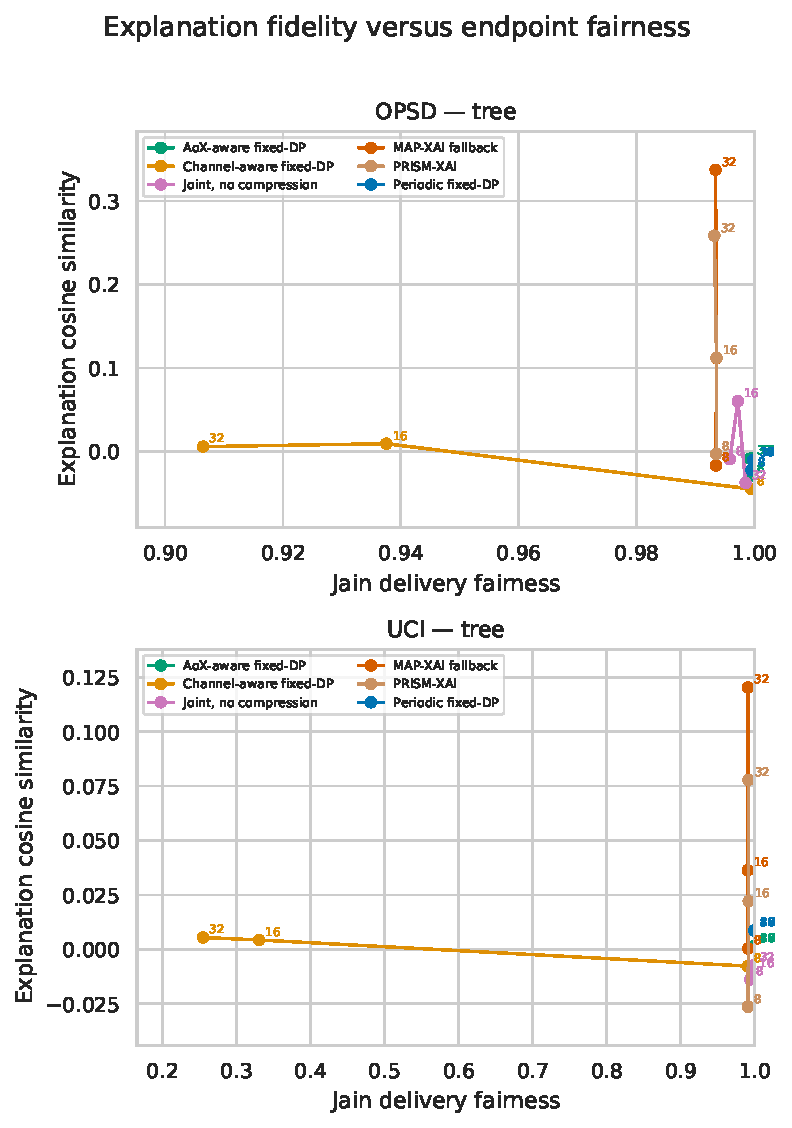
\includegraphics[width=.96\textwidth,height=.82\textheight,keepaspectratio]{../../SERVICE_TRADEOFF_RESULTS/runs/thr_1_cap_8/fairness_reliability.pdf}

\caption{Public-score threshold $\tau=1$, release cap $M=8$, Combined datasets: fairness--reliability plane. This panel should be read with the setting-level quantitative interpretation and the complete tables immediately preceding the figure block.}

\end{figure*}

\clearpage

\begin{figure*}[p]

\centering

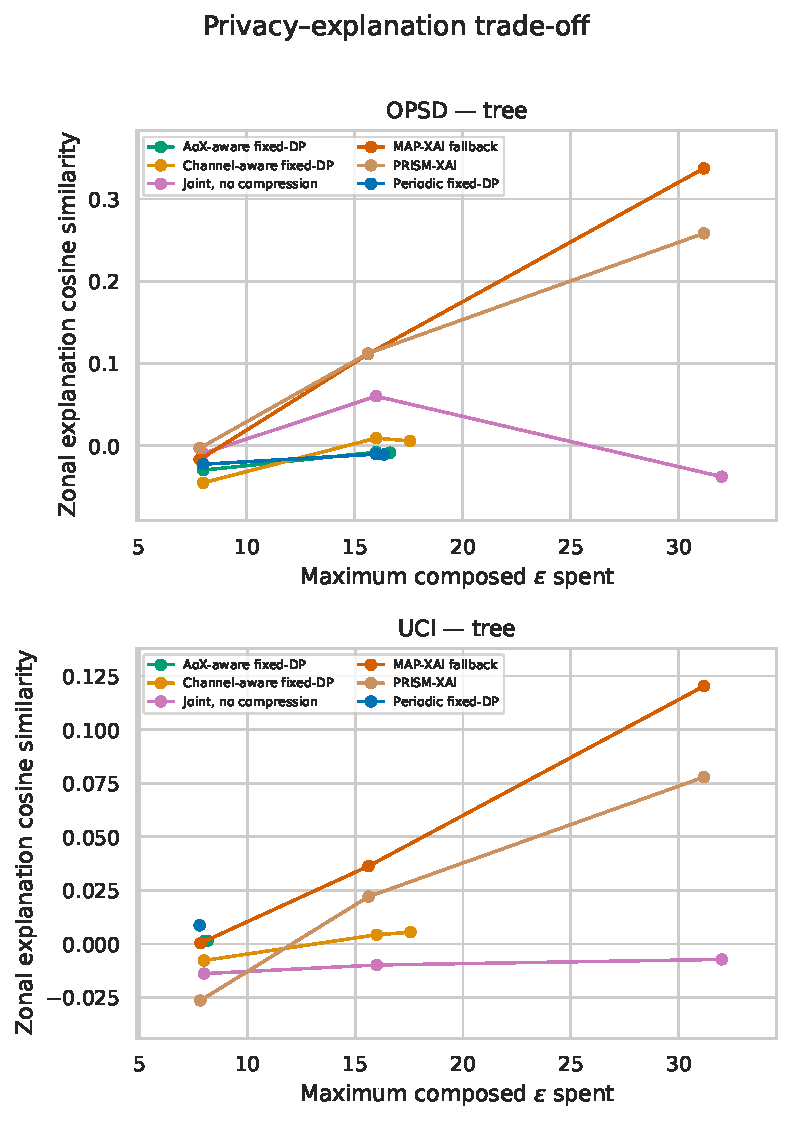
\includegraphics[width=.96\textwidth,height=.82\textheight,keepaspectratio]{../../SERVICE_TRADEOFF_RESULTS/runs/thr_1_cap_8/privacy_fidelity.pdf}

\caption{Public-score threshold $\tau=1$, release cap $M=8$, Combined datasets: privacy--fidelity plane. This panel should be read with the setting-level quantitative interpretation and the complete tables immediately preceding the figure block.}

\end{figure*}

\clearpage

\begin{figure*}[p]

\centering

\includegraphics[width=.96\textwidth,height=.82\textheight,keepaspectratio]{../../SERVICE_TRADEOFF_RESULTS/runs/thr_1_cap_8/pareto_bits_fidelity.pdf}

\caption{Public-score threshold $\tau=1$, release cap $M=8$, Combined datasets: traffic--fidelity Pareto plane. This panel should be read with the setting-level quantitative interpretation and the complete tables immediately preceding the figure block.}

\end{figure*}

\clearpage

\begin{figure*}[p]

\centering

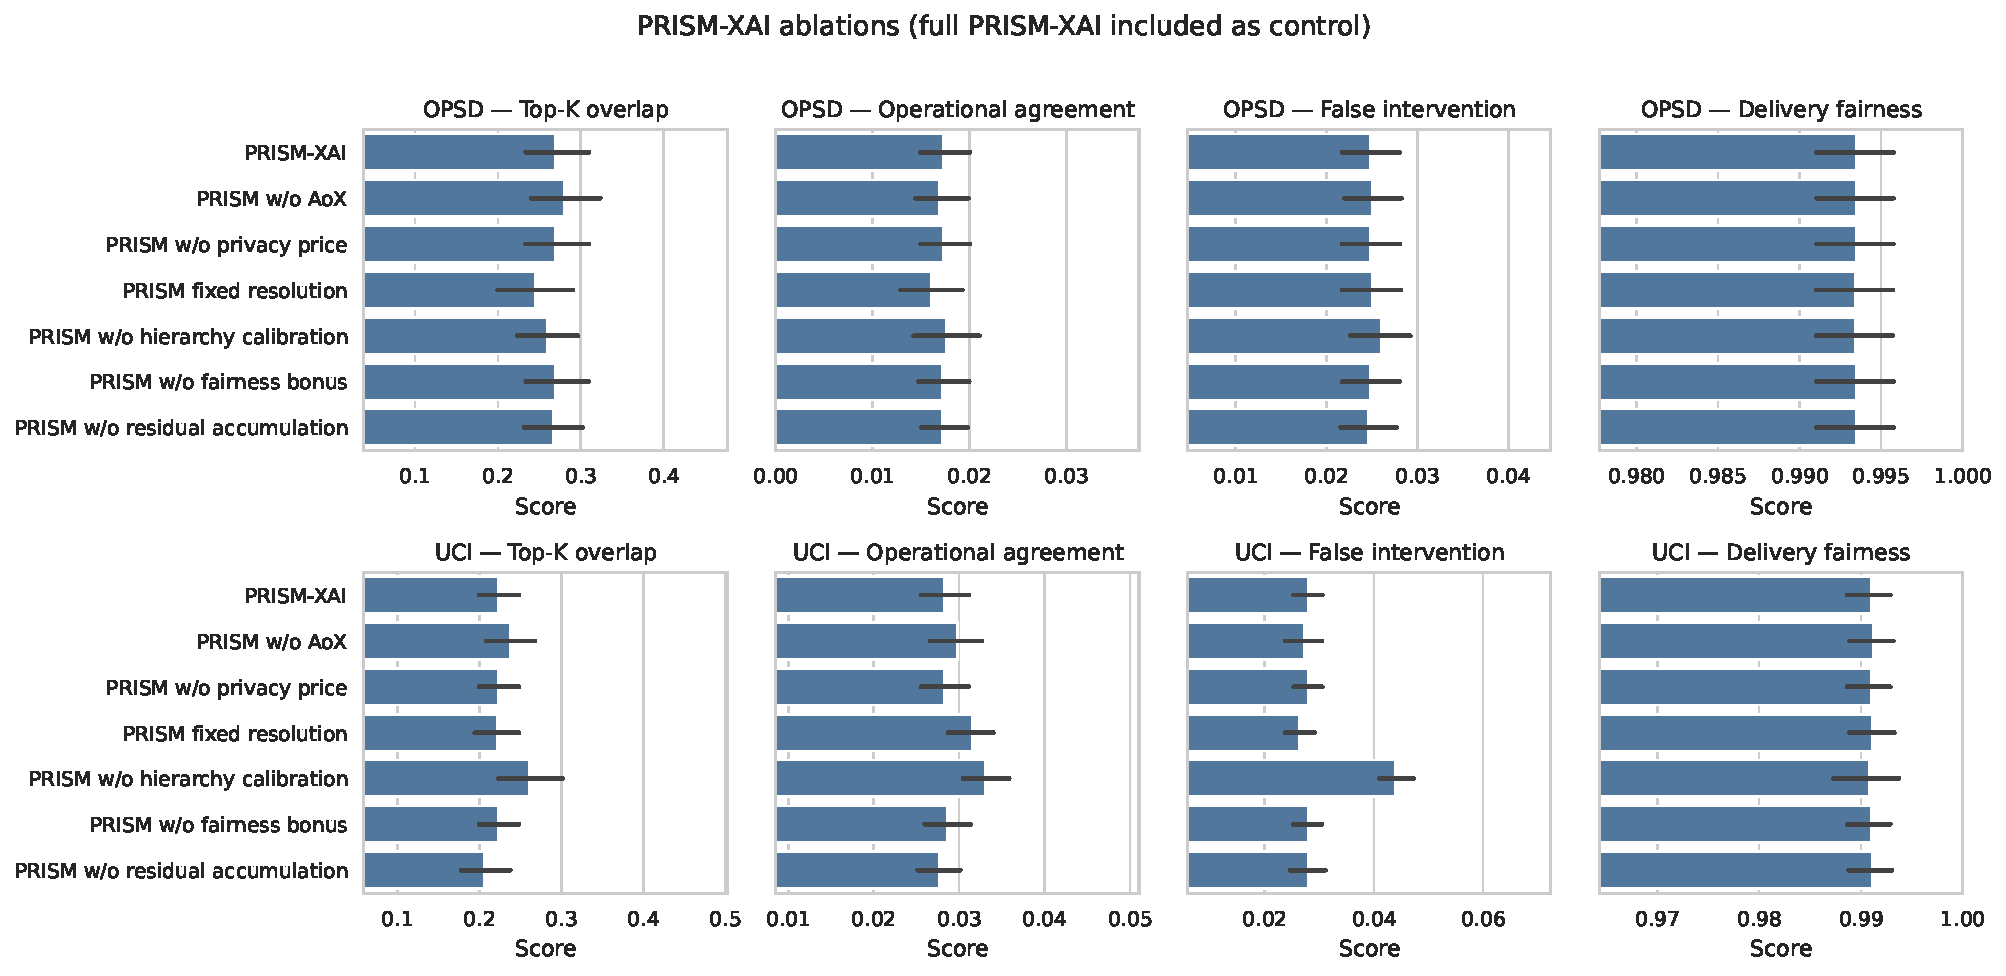
\includegraphics[width=.96\textwidth,height=.82\textheight,keepaspectratio]{../../SERVICE_TRADEOFF_RESULTS/runs/thr_1_cap_8/ablation_results.pdf}

\caption{Public-score threshold $\tau=1$, release cap $M=8$, Combined datasets: component ablation. This panel should be read with the setting-level quantitative interpretation and the complete tables immediately preceding the figure block.}

\end{figure*}

\clearpage

\paragraph{OPSD.} The three generated tables below report the full method means, all condition-level values, and paired differences. The five figures that follow provide the corresponding temporal, fairness, privacy, Pareto, and ablation views. Aggregate panels support the setting-level summary above; dataset panels reveal whether that summary is shared by OPSD and UCI rather than being driven by their different endpoint counts.

\begin{table*}[p]\centering\tiny

\caption{Public-score threshold $\tau=1$, release cap $M=8$, OPSD: complete generated method table.}

\label{tab:thr_1_cap_8:opsd:main}

\resizebox{\linewidth}{!}{% Values are means with 95% Student-t confidence intervals across seeds.
\begin{tabular}{lccccccccccccccc}
\toprule
Dataset & Model & $\epsilon_{\max}$ & Method & Top-$K$ & Cosine & Decision & Recall & Prec. & Abst. & P95 ms & kbit & Spent $\epsilon$ & False int. & bit/correct & Fairness \\
\midrule
OPSD & Tree & 8 & AoX-aware fixed-DP & 0.234 $\pm$ 0.048 & -0.033 $\pm$ 0.028 & 0.119 $\pm$ 0.028 & 0.119 $\pm$ 0.028 & 0.198 $\pm$ 0.054 & 0.721 $\pm$ 0.005 & 6.903 $\pm$ 1.126 & 1560.564 $\pm$ 0.000 & 7.990 $\pm$ 0.000 & 0.183 $\pm$ 0.020 & 35567.482 $\pm$ 10569.818 & 0.999 $\pm$ 0.000 \\
OPSD & Tree & 8 & AoX-aware fixed-DP & 0.238 $\pm$ 0.049 & -0.026 $\pm$ 0.055 & 0.121 $\pm$ 0.026 & 0.121 $\pm$ 0.026 & 0.205 $\pm$ 0.053 & 0.721 $\pm$ 0.005 & 6.903 $\pm$ 1.126 & 1560.564 $\pm$ 0.000 & 7.990 $\pm$ 0.000 & 0.179 $\pm$ 0.023 & 34123.214 $\pm$ 8376.542 & 0.999 $\pm$ 0.000 \\
OPSD & Tree & 8 & Channel-aware fixed-DP & 0.292 $\pm$ 0.037 & -0.041 $\pm$ 0.051 & 0.107 $\pm$ 0.026 & 0.107 $\pm$ 0.026 & 0.217 $\pm$ 0.068 & 0.779 $\pm$ 0.011 & 5.571 $\pm$ 1.784 & 1560.564 $\pm$ 0.000 & 7.990 $\pm$ 0.000 & 0.154 $\pm$ 0.029 & 40860.756 $\pm$ 14126.920 & 0.999 $\pm$ 0.000 \\
OPSD & Tree & 8 & Channel-aware fixed-DP & 0.292 $\pm$ 0.054 & -0.049 $\pm$ 0.064 & 0.111 $\pm$ 0.023 & 0.111 $\pm$ 0.023 & 0.228 $\pm$ 0.066 & 0.779 $\pm$ 0.011 & 5.571 $\pm$ 1.784 & 1560.564 $\pm$ 0.000 & 7.990 $\pm$ 0.000 & 0.149 $\pm$ 0.026 & 37980.855 $\pm$ 12338.094 & 0.999 $\pm$ 0.000 \\
OPSD & Tree & 8 & Joint, no compression & 0.288 $\pm$ 0.064 & -0.030 $\pm$ 0.079 & 0.016 $\pm$ 0.005 & 0.016 $\pm$ 0.005 & 0.193 $\pm$ 0.059 & 0.957 $\pm$ 0.003 & 4.560 $\pm$ 1.811 & 189.900 $\pm$ 0.554 & 7.990 $\pm$ 0.000 & 0.027 $\pm$ 0.005 & 32490.357 $\pm$ 10149.755 & 0.996 $\pm$ 0.002 \\
OPSD & Tree & 8 & Joint, no compression & 0.258 $\pm$ 0.055 & 0.011 $\pm$ 0.094 & 0.019 $\pm$ 0.004 & 0.019 $\pm$ 0.004 & 0.224 $\pm$ 0.044 & 0.957 $\pm$ 0.003 & 4.562 $\pm$ 1.809 & 189.750 $\pm$ 0.566 & 7.990 $\pm$ 0.000 & 0.025 $\pm$ 0.003 & 26079.167 $\pm$ 6335.386 & 0.996 $\pm$ 0.002 \\
OPSD & Tree & 8 & Periodic fixed-DP & 0.241 $\pm$ 0.049 & -0.019 $\pm$ 0.061 & 0.125 $\pm$ 0.020 & 0.125 $\pm$ 0.020 & 0.209 $\pm$ 0.044 & 0.722 $\pm$ 0.006 & 6.303 $\pm$ 1.438 & 1560.564 $\pm$ 0.000 & 7.990 $\pm$ 0.000 & 0.181 $\pm$ 0.021 & 31183.082 $\pm$ 4356.378 & 0.999 $\pm$ 0.000 \\
OPSD & Tree & 8 & Periodic fixed-DP & 0.242 $\pm$ 0.048 & -0.026 $\pm$ 0.082 & 0.135 $\pm$ 0.016 & 0.135 $\pm$ 0.016 & 0.231 $\pm$ 0.037 & 0.722 $\pm$ 0.006 & 6.303 $\pm$ 1.438 & 1560.564 $\pm$ 0.000 & 7.990 $\pm$ 0.000 & 0.169 $\pm$ 0.017 & 28520.235 $\pm$ 3511.595 & 0.999 $\pm$ 0.000 \\
OPSD & Tree & 8 & PRISM-XAI & 0.271 $\pm$ 0.064 & -0.008 $\pm$ 0.077 & 0.018 $\pm$ 0.004 & 0.018 $\pm$ 0.004 & 0.219 $\pm$ 0.073 & 0.956 $\pm$ 0.003 & 4.630 $\pm$ 1.839 & 87.543 $\pm$ 0.387 & 7.823 $\pm$ 0.000 & 0.026 $\pm$ 0.006 & 12978.492 $\pm$ 2874.959 & 0.993 $\pm$ 0.004 \\
OPSD & Tree & 8 & PRISM-XAI & 0.269 $\pm$ 0.071 & 0.002 $\pm$ 0.071 & 0.017 $\pm$ 0.005 & 0.017 $\pm$ 0.005 & 0.217 $\pm$ 0.065 & 0.956 $\pm$ 0.003 & 4.622 $\pm$ 1.845 & 87.369 $\pm$ 0.346 & 7.823 $\pm$ 0.000 & 0.024 $\pm$ 0.005 & 13859.274 $\pm$ 3369.246 & 0.994 $\pm$ 0.004 \\
OPSD & Tree & 8 & MAP-XAI fallback & 0.225 $\pm$ 0.063 & -0.029 $\pm$ 0.071 & 0.015 $\pm$ 0.006 & 0.015 $\pm$ 0.006 & 0.190 $\pm$ 0.076 & 0.956 $\pm$ 0.003 & 4.732 $\pm$ 1.776 & 105.817 $\pm$ 0.049 & 7.823 $\pm$ 0.000 & 0.026 $\pm$ 0.006 & 22620.844 $\pm$ 10124.929 & 0.993 $\pm$ 0.004 \\
OPSD & Tree & 8 & MAP-XAI fallback & 0.251 $\pm$ 0.064 & -0.005 $\pm$ 0.077 & 0.017 $\pm$ 0.006 & 0.017 $\pm$ 0.006 & 0.217 $\pm$ 0.076 & 0.956 $\pm$ 0.003 & 4.732 $\pm$ 1.776 & 105.675 $\pm$ 0.049 & 7.823 $\pm$ 0.000 & 0.024 $\pm$ 0.006 & 18265.481 $\pm$ 6339.471 & 0.993 $\pm$ 0.004 \\
\bottomrule
\end{tabular}
}

\end{table*}\clearpage

\begin{table*}[p]\centering\tiny

\caption{Public-score threshold $\tau=1$, release cap $M=8$, OPSD: complete condition-level generated table.}

\label{tab:thr_1_cap_8:opsd:conditions}

\resizebox{\textwidth}{!}{\begin{tabular}{llllccccccccccc}
\toprule
Dataset & Model & $\epsilon_{\max}$ & Method & kbit & Top-$K$ & Random Top-$K$ & Cosine & Decision & Recall & Precision & Coverage & Abstain & False int. & Spent $\epsilon$ \\
\midrule
OPSD & Tree & 8 & Joint, no compression & 189.900 $\pm$ 0.554 & 0.288 $\pm$ 0.064 & 0.250 $\pm$ 0.000 & -0.030 $\pm$ 0.079 & 0.016 $\pm$ 0.005 & 0.016 $\pm$ 0.005 & 0.193 $\pm$ 0.059 & 0.043 $\pm$ 0.003 & 0.957 $\pm$ 0.003 & 0.027 $\pm$ 0.005 & 7.990 $\pm$ 0.000 \\
OPSD & Tree & 8 & Joint, no compression & 189.750 $\pm$ 0.566 & 0.258 $\pm$ 0.055 & 0.250 $\pm$ 0.000 & 0.011 $\pm$ 0.094 & 0.019 $\pm$ 0.004 & 0.019 $\pm$ 0.004 & 0.224 $\pm$ 0.044 & 0.043 $\pm$ 0.003 & 0.957 $\pm$ 0.003 & 0.025 $\pm$ 0.003 & 7.990 $\pm$ 0.000 \\
OPSD & Tree & 8 & Periodic fixed-DP & 1560.564 $\pm$ 0.000 & 0.241 $\pm$ 0.049 & 0.250 $\pm$ 0.000 & -0.019 $\pm$ 0.061 & 0.125 $\pm$ 0.020 & 0.125 $\pm$ 0.020 & 0.209 $\pm$ 0.044 & 0.278 $\pm$ 0.006 & 0.722 $\pm$ 0.006 & 0.181 $\pm$ 0.021 & 7.990 $\pm$ 0.000 \\
OPSD & Tree & 8 & Periodic fixed-DP & 1560.564 $\pm$ 0.000 & 0.242 $\pm$ 0.048 & 0.250 $\pm$ 0.000 & -0.026 $\pm$ 0.082 & 0.135 $\pm$ 0.016 & 0.135 $\pm$ 0.016 & 0.231 $\pm$ 0.037 & 0.278 $\pm$ 0.006 & 0.722 $\pm$ 0.006 & 0.169 $\pm$ 0.017 & 7.990 $\pm$ 0.000 \\
OPSD & Tree & 8 & PRISM-XAI & 87.543 $\pm$ 0.387 & 0.271 $\pm$ 0.064 & 0.250 $\pm$ 0.000 & -0.008 $\pm$ 0.077 & 0.018 $\pm$ 0.004 & 0.018 $\pm$ 0.004 & 0.219 $\pm$ 0.073 & 0.044 $\pm$ 0.003 & 0.956 $\pm$ 0.003 & 0.026 $\pm$ 0.006 & 7.823 $\pm$ 0.000 \\
OPSD & Tree & 8 & PRISM-XAI & 87.369 $\pm$ 0.346 & 0.269 $\pm$ 0.071 & 0.250 $\pm$ 0.000 & 0.002 $\pm$ 0.071 & 0.017 $\pm$ 0.005 & 0.017 $\pm$ 0.005 & 0.217 $\pm$ 0.065 & 0.044 $\pm$ 0.003 & 0.956 $\pm$ 0.003 & 0.024 $\pm$ 0.005 & 7.823 $\pm$ 0.000 \\
OPSD & Tree & 16 & Joint, no compression & 459.900 $\pm$ 0.750 & 0.232 $\pm$ 0.065 & 0.250 $\pm$ 0.000 & 0.059 $\pm$ 0.048 & 0.038 $\pm$ 0.009 & 0.038 $\pm$ 0.009 & 0.222 $\pm$ 0.049 & 0.088 $\pm$ 0.004 & 0.912 $\pm$ 0.004 & 0.049 $\pm$ 0.005 & 15.997 $\pm$ 0.000 \\
OPSD & Tree & 16 & Joint, no compression & 460.050 $\pm$ 0.724 & 0.241 $\pm$ 0.055 & 0.250 $\pm$ 0.000 & 0.061 $\pm$ 0.052 & 0.039 $\pm$ 0.008 & 0.039 $\pm$ 0.008 & 0.241 $\pm$ 0.042 & 0.088 $\pm$ 0.004 & 0.912 $\pm$ 0.004 & 0.045 $\pm$ 0.004 & 15.997 $\pm$ 0.000 \\
OPSD & Tree & 16 & Periodic fixed-DP & 5112.594 $\pm$ 0.000 & 0.249 $\pm$ 0.022 & 0.250 $\pm$ 0.000 & -0.009 $\pm$ 0.045 & 0.450 $\pm$ 0.062 & 0.450 $\pm$ 0.062 & 0.237 $\pm$ 0.042 & 0.985 $\pm$ 0.002 & 0.015 $\pm$ 0.002 & 0.551 $\pm$ 0.057 & 15.997 $\pm$ 0.000 \\
OPSD & Tree & 16 & Periodic fixed-DP & 5112.594 $\pm$ 0.000 & 0.243 $\pm$ 0.019 & 0.250 $\pm$ 0.000 & -0.012 $\pm$ 0.050 & 0.463 $\pm$ 0.047 & 0.463 $\pm$ 0.047 & 0.240 $\pm$ 0.028 & 0.985 $\pm$ 0.002 & 0.015 $\pm$ 0.002 & 0.547 $\pm$ 0.036 & 15.997 $\pm$ 0.000 \\
OPSD & Tree & 16 & PRISM-XAI & 87.513 $\pm$ 0.398 & 0.282 $\pm$ 0.051 & 0.250 $\pm$ 0.000 & 0.088 $\pm$ 0.071 & 0.018 $\pm$ 0.005 & 0.018 $\pm$ 0.005 & 0.230 $\pm$ 0.080 & 0.044 $\pm$ 0.003 & 0.956 $\pm$ 0.003 & 0.024 $\pm$ 0.006 & 15.620 $\pm$ 0.000 \\
OPSD & Tree & 16 & PRISM-XAI & 87.369 $\pm$ 0.313 & 0.275 $\pm$ 0.076 & 0.250 $\pm$ 0.000 & 0.136 $\pm$ 0.053 & 0.018 $\pm$ 0.006 & 0.018 $\pm$ 0.006 & 0.236 $\pm$ 0.080 & 0.044 $\pm$ 0.003 & 0.956 $\pm$ 0.003 & 0.024 $\pm$ 0.006 & 15.620 $\pm$ 0.000 \\
OPSD & Tree & 32 & Joint, no compression & 1140.900 $\pm$ 7.953 & 0.235 $\pm$ 0.064 & 0.250 $\pm$ 0.000 & -0.031 $\pm$ 0.089 & 0.074 $\pm$ 0.015 & 0.074 $\pm$ 0.015 & 0.205 $\pm$ 0.039 & 0.157 $\pm$ 0.006 & 0.843 $\pm$ 0.006 & 0.107 $\pm$ 0.009 & 31.999 $\pm$ 0.000 \\
OPSD & Tree & 32 & Joint, no compression & 1140.900 $\pm$ 7.953 & 0.282 $\pm$ 0.054 & 0.250 $\pm$ 0.000 & -0.044 $\pm$ 0.076 & 0.080 $\pm$ 0.011 & 0.080 $\pm$ 0.011 & 0.227 $\pm$ 0.052 & 0.158 $\pm$ 0.006 & 0.842 $\pm$ 0.006 & 0.105 $\pm$ 0.015 & 31.999 $\pm$ 0.000 \\
OPSD & Tree & 32 & Periodic fixed-DP & 5299.836 $\pm$ 0.625 & 0.249 $\pm$ 0.022 & 0.250 $\pm$ 0.000 & -0.009 $\pm$ 0.044 & 0.458 $\pm$ 0.066 & 0.458 $\pm$ 0.066 & 0.237 $\pm$ 0.045 & 1.000 $\pm$ 0.000 & 0.000 $\pm$ 0.000 & 0.562 $\pm$ 0.062 & 16.371 $\pm$ 0.000 \\
OPSD & Tree & 32 & Periodic fixed-DP & 5299.836 $\pm$ 0.625 & 0.244 $\pm$ 0.019 & 0.250 $\pm$ 0.000 & -0.012 $\pm$ 0.050 & 0.471 $\pm$ 0.049 & 0.471 $\pm$ 0.049 & 0.240 $\pm$ 0.029 & 1.000 $\pm$ 0.000 & 0.000 $\pm$ 0.000 & 0.559 $\pm$ 0.039 & 16.371 $\pm$ 0.000 \\
OPSD & Tree & 32 & PRISM-XAI & 87.482 $\pm$ 0.366 & 0.365 $\pm$ 0.069 & 0.250 $\pm$ 0.000 & 0.225 $\pm$ 0.051 & 0.022 $\pm$ 0.005 & 0.022 $\pm$ 0.005 & 0.373 $\pm$ 0.132 & 0.044 $\pm$ 0.003 & 0.956 $\pm$ 0.003 & 0.015 $\pm$ 0.005 & 31.175 $\pm$ 0.000 \\
OPSD & Tree & 32 & PRISM-XAI & 87.185 $\pm$ 0.219 & 0.398 $\pm$ 0.060 & 0.250 $\pm$ 0.000 & 0.291 $\pm$ 0.044 & 0.022 $\pm$ 0.005 & 0.022 $\pm$ 0.005 & 0.365 $\pm$ 0.152 & 0.044 $\pm$ 0.003 & 0.956 $\pm$ 0.003 & 0.017 $\pm$ 0.006 & 31.175 $\pm$ 0.000 \\
\bottomrule
\end{tabular}
}

\end{table*}\clearpage

\begin{table*}[p]\centering\tiny

\caption{Public-score threshold $\tau=1$, release cap $M=8$, OPSD: complete generated paired comparisons.}

\label{tab:thr_1_cap_8:opsd:paired}

\resizebox{\textwidth}{!}{\begin{tabular}{llcccc}
\toprule
Dataset & Baseline & Delta kbit & Delta Top-$K$ & Delta recall & Delta fairness \\
\midrule
OPSD & AoX-aware fixed-DP & -1473.021 $\pm$ 0.387 & 0.037 $\pm$ 0.076 & -0.102 $\pm$ 0.029 & -0.006 $\pm$ 0.004 \\
OPSD & AoX-aware fixed-DP & -5012.400 $\pm$ 5.552 & 0.029 $\pm$ 0.064 & -0.383 $\pm$ 0.074 & -0.006 $\pm$ 0.004 \\
OPSD & AoX-aware fixed-DP & -5212.742 $\pm$ 0.366 & 0.112 $\pm$ 0.088 & -0.391 $\pm$ 0.079 & -0.006 $\pm$ 0.005 \\
OPSD & AoX-aware fixed-DP & -1473.195 $\pm$ 0.346 & 0.030 $\pm$ 0.077 & -0.104 $\pm$ 0.026 & -0.006 $\pm$ 0.004 \\
OPSD & AoX-aware fixed-DP & -5012.544 $\pm$ 5.514 & 0.023 $\pm$ 0.077 & -0.396 $\pm$ 0.057 & -0.006 $\pm$ 0.004 \\
OPSD & AoX-aware fixed-DP & -5213.039 $\pm$ 0.219 & 0.147 $\pm$ 0.078 & -0.403 $\pm$ 0.059 & -0.006 $\pm$ 0.005 \\
OPSD & Channel-aware fixed-DP & -1473.021 $\pm$ 0.387 & -0.021 $\pm$ 0.081 & -0.089 $\pm$ 0.026 & -0.006 $\pm$ 0.004 \\
OPSD & Channel-aware fixed-DP & -4599.097 $\pm$ 12.954 & 0.021 $\pm$ 0.063 & -0.383 $\pm$ 0.090 & 0.056 $\pm$ 0.006 \\
OPSD & Channel-aware fixed-DP & -5212.742 $\pm$ 0.366 & 0.107 $\pm$ 0.084 & -0.413 $\pm$ 0.099 & 0.087 $\pm$ 0.007 \\
OPSD & Channel-aware fixed-DP & -1473.195 $\pm$ 0.346 & -0.024 $\pm$ 0.075 & -0.094 $\pm$ 0.023 & -0.006 $\pm$ 0.004 \\
OPSD & Channel-aware fixed-DP & -4599.240 $\pm$ 12.910 & 0.017 $\pm$ 0.079 & -0.401 $\pm$ 0.088 & 0.056 $\pm$ 0.006 \\
OPSD & Channel-aware fixed-DP & -5213.039 $\pm$ 0.219 & 0.141 $\pm$ 0.071 & -0.434 $\pm$ 0.092 & 0.087 $\pm$ 0.007 \\
OPSD & Joint, no compression & -102.357 $\pm$ 0.507 & -0.017 $\pm$ 0.096 & 0.001 $\pm$ 0.004 & -0.002 $\pm$ 0.003 \\
OPSD & Joint, no compression & -372.387 $\pm$ 1.050 & 0.051 $\pm$ 0.071 & -0.020 $\pm$ 0.010 & -0.004 $\pm$ 0.004 \\
OPSD & Joint, no compression & -1053.418 $\pm$ 7.970 & 0.129 $\pm$ 0.123 & -0.052 $\pm$ 0.014 & -0.005 $\pm$ 0.005 \\
OPSD & Joint, no compression & -102.381 $\pm$ 0.421 & 0.010 $\pm$ 0.097 & -0.002 $\pm$ 0.003 & -0.002 $\pm$ 0.003 \\
OPSD & Joint, no compression & -372.681 $\pm$ 0.901 & 0.035 $\pm$ 0.072 & -0.020 $\pm$ 0.008 & -0.004 $\pm$ 0.004 \\
OPSD & Joint, no compression & -1053.715 $\pm$ 7.867 & 0.116 $\pm$ 0.104 & -0.058 $\pm$ 0.012 & -0.005 $\pm$ 0.005 \\
OPSD & Periodic fixed-DP & -1473.021 $\pm$ 0.387 & 0.031 $\pm$ 0.076 & -0.107 $\pm$ 0.021 & -0.006 $\pm$ 0.004 \\
OPSD & Periodic fixed-DP & -5025.081 $\pm$ 0.398 & 0.033 $\pm$ 0.059 & -0.432 $\pm$ 0.063 & -0.006 $\pm$ 0.004 \\
OPSD & Periodic fixed-DP & -5212.354 $\pm$ 0.641 & 0.116 $\pm$ 0.083 & -0.436 $\pm$ 0.068 & -0.007 $\pm$ 0.005 \\
OPSD & Periodic fixed-DP & -1473.195 $\pm$ 0.346 & 0.027 $\pm$ 0.083 & -0.118 $\pm$ 0.016 & -0.006 $\pm$ 0.004 \\
OPSD & Periodic fixed-DP & -5025.225 $\pm$ 0.313 & 0.032 $\pm$ 0.072 & -0.444 $\pm$ 0.049 & -0.006 $\pm$ 0.004 \\
OPSD & Periodic fixed-DP & -5212.651 $\pm$ 0.592 & 0.155 $\pm$ 0.065 & -0.449 $\pm$ 0.050 & -0.007 $\pm$ 0.005 \\
OPSD & MAP-XAI fallback & -18.273 $\pm$ 0.401 & 0.046 $\pm$ 0.070 & 0.002 $\pm$ 0.003 & 0.000 $\pm$ 0.000 \\
OPSD & MAP-XAI fallback & -18.304 $\pm$ 0.409 & 0.038 $\pm$ 0.045 & 0.001 $\pm$ 0.006 & 0.000 $\pm$ 0.000 \\
OPSD & MAP-XAI fallback & -18.335 $\pm$ 0.374 & 0.013 $\pm$ 0.060 & -0.002 $\pm$ 0.005 & -0.000 $\pm$ 0.001 \\
OPSD & MAP-XAI fallback & -18.306 $\pm$ 0.346 & 0.018 $\pm$ 0.054 & 0.000 $\pm$ 0.004 & 0.000 $\pm$ 0.000 \\
OPSD & MAP-XAI fallback & -18.285 $\pm$ 0.309 & 0.011 $\pm$ 0.065 & -0.000 $\pm$ 0.005 & 0.000 $\pm$ 0.000 \\
OPSD & MAP-XAI fallback & -18.367 $\pm$ 0.250 & 0.022 $\pm$ 0.068 & -0.002 $\pm$ 0.003 & -0.000 $\pm$ 0.000 \\
\bottomrule
\end{tabular}
}

\end{table*}\clearpage

\begin{figure*}[p]

\centering

\includegraphics[width=.96\textwidth,height=.82\textheight,keepaspectratio]{../../SERVICE_TRADEOFF_RESULTS/runs/thr_1_cap_8/opsd/regime_trace.pdf}

\caption{Public-score threshold $\tau=1$, release cap $M=8$, OPSD: representative regime trace. This panel should be read with the setting-level quantitative interpretation and the complete tables immediately preceding the figure block.}

\end{figure*}

\clearpage

\begin{figure*}[p]

\centering

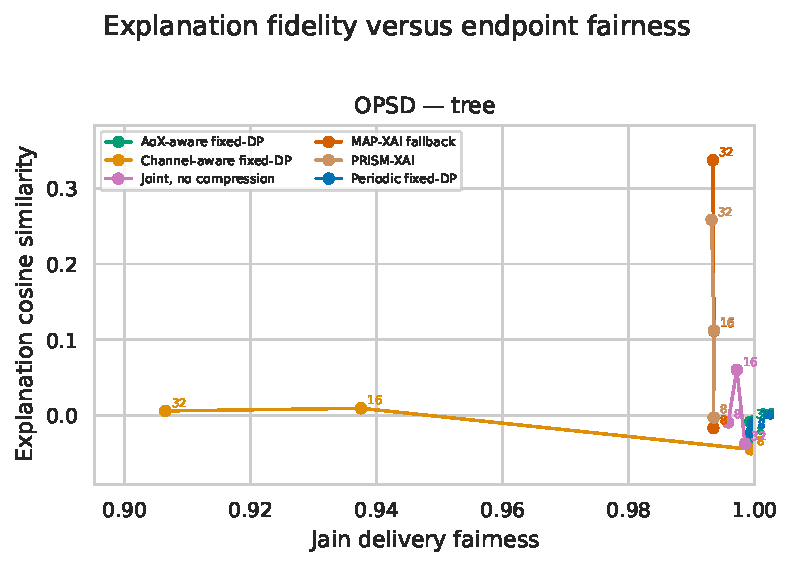
\includegraphics[width=.96\textwidth,height=.82\textheight,keepaspectratio]{../../SERVICE_TRADEOFF_RESULTS/runs/thr_1_cap_8/opsd/fairness_reliability.pdf}

\caption{Public-score threshold $\tau=1$, release cap $M=8$, OPSD: fairness--reliability plane. This panel should be read with the setting-level quantitative interpretation and the complete tables immediately preceding the figure block.}

\end{figure*}

\clearpage

\begin{figure*}[p]

\centering

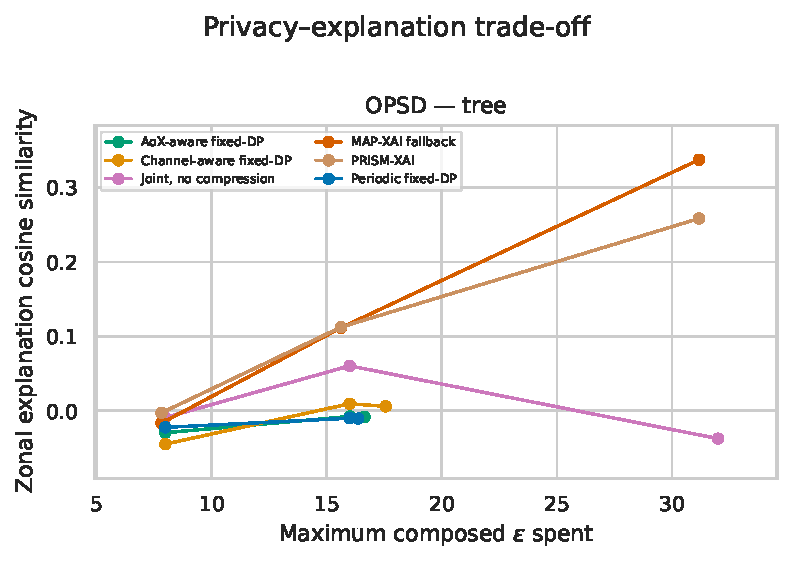
\includegraphics[width=.96\textwidth,height=.82\textheight,keepaspectratio]{../../SERVICE_TRADEOFF_RESULTS/runs/thr_1_cap_8/opsd/privacy_fidelity.pdf}

\caption{Public-score threshold $\tau=1$, release cap $M=8$, OPSD: privacy--fidelity plane. This panel should be read with the setting-level quantitative interpretation and the complete tables immediately preceding the figure block.}

\end{figure*}

\clearpage

\begin{figure*}[p]

\centering

\includegraphics[width=.96\textwidth,height=.82\textheight,keepaspectratio]{../../SERVICE_TRADEOFF_RESULTS/runs/thr_1_cap_8/opsd/pareto_bits_fidelity.pdf}

\caption{Public-score threshold $\tau=1$, release cap $M=8$, OPSD: traffic--fidelity Pareto plane. This panel should be read with the setting-level quantitative interpretation and the complete tables immediately preceding the figure block.}

\end{figure*}

\clearpage

\begin{figure*}[p]

\centering

\includegraphics[width=.96\textwidth,height=.82\textheight,keepaspectratio]{../../SERVICE_TRADEOFF_RESULTS/runs/thr_1_cap_8/opsd/ablation_results.pdf}

\caption{Public-score threshold $\tau=1$, release cap $M=8$, OPSD: component ablation. This panel should be read with the setting-level quantitative interpretation and the complete tables immediately preceding the figure block.}

\end{figure*}

\clearpage

\paragraph{UCI.} The three generated tables below report the full method means, all condition-level values, and paired differences. The five figures that follow provide the corresponding temporal, fairness, privacy, Pareto, and ablation views. Aggregate panels support the setting-level summary above; dataset panels reveal whether that summary is shared by OPSD and UCI rather than being driven by their different endpoint counts.

\begin{table*}[p]\centering\tiny

\caption{Public-score threshold $\tau=1$, release cap $M=8$, UCI: complete generated method table.}

\label{tab:thr_1_cap_8:uci:main}

\resizebox{\linewidth}{!}{% Values are means with 95% Student-t confidence intervals across seeds.
\begin{tabular}{lccccccccccccccc}
\toprule
Dataset & Model & $\epsilon_{\max}$ & Method & Top-$K$ & Cosine & Decision & Recall & Prec. & Abst. & P95 ms & kbit & Spent $\epsilon$ & False int. & bit/correct & Fairness \\
\midrule
UCI & Tree & 8 & AoX-aware fixed-DP & 0.263 $\pm$ 0.041 & -0.007 $\pm$ 0.009 & 0.457 $\pm$ 0.031 & 0.457 $\pm$ 0.031 & 0.362 $\pm$ 0.024 & 0.003 $\pm$ 0.001 & 7.500 $\pm$ 0.000 & 5300.224 $\pm$ 0.000 & 7.990 $\pm$ 0.000 & 0.557 $\pm$ 0.025 & 14002.896 $\pm$ 1040.243 & 0.999 $\pm$ 0.000 \\
UCI & Tree & 8 & AoX-aware fixed-DP & 0.260 $\pm$ 0.022 & 0.010 $\pm$ 0.055 & 0.455 $\pm$ 0.047 & 0.455 $\pm$ 0.047 & 0.361 $\pm$ 0.038 & 0.003 $\pm$ 0.001 & 7.500 $\pm$ 0.000 & 5300.224 $\pm$ 0.000 & 7.990 $\pm$ 0.000 & 0.557 $\pm$ 0.048 & 14198.303 $\pm$ 1508.274 & 0.999 $\pm$ 0.000 \\
UCI & Tree & 8 & Channel-aware fixed-DP & 0.248 $\pm$ 0.031 & 0.004 $\pm$ 0.012 & 0.001 $\pm$ 0.001 & 0.001 $\pm$ 0.001 & 0.150 $\pm$ 0.151 & 0.999 $\pm$ 0.001 & 4.609 $\pm$ 1.781 & 5295.177 $\pm$ 3.740 & 7.990 $\pm$ 0.000 & 0.001 $\pm$ 0.001 & 4632196.500 $\pm$ 2102650.252 & 0.991 $\pm$ 0.001 \\
UCI & Tree & 8 & Channel-aware fixed-DP & 0.239 $\pm$ 0.030 & -0.020 $\pm$ 0.055 & 0.000 $\pm$ 0.000 & 0.000 $\pm$ 0.000 & 0.117 $\pm$ 0.225 & 0.999 $\pm$ 0.001 & 4.609 $\pm$ 1.781 & 5295.177 $\pm$ 3.740 & 7.990 $\pm$ 0.000 & 0.001 $\pm$ 0.001 & 5296989.000 $\pm$ 41104.572 & 0.991 $\pm$ 0.001 \\
UCI & Tree & 8 & Joint, no compression & 0.286 $\pm$ 0.045 & 0.004 $\pm$ 0.020 & 0.052 $\pm$ 0.005 & 0.052 $\pm$ 0.005 & 0.406 $\pm$ 0.037 & 0.875 $\pm$ 0.003 & 5.123 $\pm$ 1.792 & 672.300 $\pm$ 0.452 & 7.990 $\pm$ 0.000 & 0.053 $\pm$ 0.004 & 15676.175 $\pm$ 1475.621 & 0.994 $\pm$ 0.003 \\
UCI & Tree & 8 & Joint, no compression & 0.229 $\pm$ 0.052 & -0.032 $\pm$ 0.050 & 0.057 $\pm$ 0.007 & 0.057 $\pm$ 0.007 & 0.428 $\pm$ 0.041 & 0.875 $\pm$ 0.003 & 5.131 $\pm$ 1.787 & 672.300 $\pm$ 0.452 & 7.990 $\pm$ 0.000 & 0.052 $\pm$ 0.004 & 14702.786 $\pm$ 2334.488 & 0.994 $\pm$ 0.003 \\
UCI & Tree & 8 & Periodic fixed-DP & 0.259 $\pm$ 0.060 & -0.005 $\pm$ 0.008 & 0.006 $\pm$ 0.001 & 0.006 $\pm$ 0.001 & 0.244 $\pm$ 0.049 & 0.989 $\pm$ 0.001 & 4.596 $\pm$ 1.788 & 5299.318 $\pm$ 1.451 & 7.786 $\pm$ 0.000 & 0.013 $\pm$ 0.002 & 1215103.896 $\pm$ 390671.319 & 0.999 $\pm$ 0.000 \\
UCI & Tree & 8 & Periodic fixed-DP & 0.260 $\pm$ 0.044 & 0.022 $\pm$ 0.070 & 0.005 $\pm$ 0.001 & 0.005 $\pm$ 0.001 & 0.195 $\pm$ 0.050 & 0.989 $\pm$ 0.001 & 4.596 $\pm$ 1.788 & 5299.318 $\pm$ 1.451 & 7.786 $\pm$ 0.000 & 0.015 $\pm$ 0.002 & 1555837.203 $\pm$ 955472.503 & 0.999 $\pm$ 0.000 \\
UCI & Tree & 8 & PRISM-XAI & 0.228 $\pm$ 0.051 & -0.001 $\pm$ 0.021 & 0.031 $\pm$ 0.005 & 0.031 $\pm$ 0.005 & 0.433 $\pm$ 0.052 & 0.933 $\pm$ 0.005 & 4.578 $\pm$ 1.800 & 323.463 $\pm$ 1.280 & 7.823 $\pm$ 0.000 & 0.029 $\pm$ 0.005 & 12910.343 $\pm$ 2005.939 & 0.992 $\pm$ 0.002 \\
UCI & Tree & 8 & PRISM-XAI & 0.219 $\pm$ 0.034 & -0.052 $\pm$ 0.048 & 0.025 $\pm$ 0.003 & 0.025 $\pm$ 0.003 & 0.390 $\pm$ 0.053 & 0.940 $\pm$ 0.005 & 4.798 $\pm$ 1.710 & 322.302 $\pm$ 1.580 & 7.823 $\pm$ 0.000 & 0.028 $\pm$ 0.004 & 15856.808 $\pm$ 2743.852 & 0.990 $\pm$ 0.005 \\
UCI & Tree & 8 & MAP-XAI fallback & 0.220 $\pm$ 0.055 & -0.006 $\pm$ 0.023 & 0.032 $\pm$ 0.005 & 0.032 $\pm$ 0.005 & 0.453 $\pm$ 0.058 & 0.932 $\pm$ 0.004 & 4.643 $\pm$ 1.763 & 382.099 $\pm$ 0.159 & 7.823 $\pm$ 0.000 & 0.027 $\pm$ 0.004 & 14883.660 $\pm$ 3313.232 & 0.992 $\pm$ 0.002 \\
UCI & Tree & 8 & MAP-XAI fallback & 0.250 $\pm$ 0.054 & 0.006 $\pm$ 0.060 & 0.030 $\pm$ 0.005 & 0.030 $\pm$ 0.005 & 0.453 $\pm$ 0.060 & 0.935 $\pm$ 0.006 & 5.564 $\pm$ 1.788 & 381.645 $\pm$ 0.090 & 7.823 $\pm$ 0.000 & 0.025 $\pm$ 0.004 & 15932.448 $\pm$ 2964.700 & 0.990 $\pm$ 0.005 \\
\bottomrule
\end{tabular}
}

\end{table*}\clearpage

\begin{table*}[p]\centering\tiny

\caption{Public-score threshold $\tau=1$, release cap $M=8$, UCI: complete condition-level generated table.}

\label{tab:thr_1_cap_8:uci:conditions}

\resizebox{\textwidth}{!}{\begin{tabular}{llllccccccccccc}
\toprule
Dataset & Model & $\epsilon_{\max}$ & Method & kbit & Top-$K$ & Random Top-$K$ & Cosine & Decision & Recall & Precision & Coverage & Abstain & False int. & Spent $\epsilon$ \\
\midrule
UCI & Tree & 8 & Joint, no compression & 672.300 $\pm$ 0.452 & 0.286 $\pm$ 0.045 & 0.250 $\pm$ 0.000 & 0.004 $\pm$ 0.020 & 0.052 $\pm$ 0.005 & 0.052 $\pm$ 0.005 & 0.406 $\pm$ 0.037 & 0.125 $\pm$ 0.003 & 0.875 $\pm$ 0.003 & 0.053 $\pm$ 0.004 & 7.990 $\pm$ 0.000 \\
UCI & Tree & 8 & Joint, no compression & 672.300 $\pm$ 0.452 & 0.229 $\pm$ 0.052 & 0.250 $\pm$ 0.000 & -0.032 $\pm$ 0.050 & 0.057 $\pm$ 0.007 & 0.057 $\pm$ 0.007 & 0.428 $\pm$ 0.041 & 0.125 $\pm$ 0.003 & 0.875 $\pm$ 0.003 & 0.052 $\pm$ 0.004 & 7.990 $\pm$ 0.000 \\
UCI & Tree & 8 & Periodic fixed-DP & 5299.318 $\pm$ 1.451 & 0.259 $\pm$ 0.060 & 0.250 $\pm$ 0.000 & -0.005 $\pm$ 0.008 & 0.006 $\pm$ 0.001 & 0.006 $\pm$ 0.001 & 0.244 $\pm$ 0.049 & 0.011 $\pm$ 0.001 & 0.989 $\pm$ 0.001 & 0.013 $\pm$ 0.002 & 7.786 $\pm$ 0.000 \\
UCI & Tree & 8 & Periodic fixed-DP & 5299.318 $\pm$ 1.451 & 0.260 $\pm$ 0.044 & 0.250 $\pm$ 0.000 & 0.022 $\pm$ 0.070 & 0.005 $\pm$ 0.001 & 0.005 $\pm$ 0.001 & 0.195 $\pm$ 0.050 & 0.011 $\pm$ 0.001 & 0.989 $\pm$ 0.001 & 0.015 $\pm$ 0.002 & 7.786 $\pm$ 0.000 \\
UCI & Tree & 8 & PRISM-XAI & 323.463 $\pm$ 1.280 & 0.228 $\pm$ 0.051 & 0.250 $\pm$ 0.000 & -0.001 $\pm$ 0.021 & 0.031 $\pm$ 0.005 & 0.031 $\pm$ 0.005 & 0.433 $\pm$ 0.052 & 0.067 $\pm$ 0.005 & 0.933 $\pm$ 0.005 & 0.029 $\pm$ 0.005 & 7.823 $\pm$ 0.000 \\
UCI & Tree & 8 & PRISM-XAI & 322.302 $\pm$ 1.580 & 0.219 $\pm$ 0.034 & 0.250 $\pm$ 0.000 & -0.052 $\pm$ 0.048 & 0.025 $\pm$ 0.003 & 0.025 $\pm$ 0.003 & 0.390 $\pm$ 0.053 & 0.060 $\pm$ 0.005 & 0.940 $\pm$ 0.005 & 0.028 $\pm$ 0.004 & 7.823 $\pm$ 0.000 \\
UCI & Tree & 16 & Joint, no compression & 1632.150 $\pm$ 0.339 & 0.216 $\pm$ 0.041 & 0.250 $\pm$ 0.000 & 0.001 $\pm$ 0.012 & 0.094 $\pm$ 0.005 & 0.094 $\pm$ 0.005 & 0.330 $\pm$ 0.024 & 0.228 $\pm$ 0.005 & 0.772 $\pm$ 0.005 & 0.133 $\pm$ 0.010 & 15.997 $\pm$ 0.000 \\
UCI & Tree & 16 & Joint, no compression & 1632.600 $\pm$ 0.554 & 0.204 $\pm$ 0.011 & 0.250 $\pm$ 0.000 & -0.021 $\pm$ 0.033 & 0.099 $\pm$ 0.016 & 0.099 $\pm$ 0.016 & 0.347 $\pm$ 0.054 & 0.228 $\pm$ 0.005 & 0.772 $\pm$ 0.005 & 0.128 $\pm$ 0.011 & 15.997 $\pm$ 0.000 \\
UCI & Tree & 16 & Periodic fixed-DP & 5299.318 $\pm$ 1.451 & 0.259 $\pm$ 0.060 & 0.250 $\pm$ 0.000 & -0.005 $\pm$ 0.008 & 0.006 $\pm$ 0.001 & 0.006 $\pm$ 0.001 & 0.244 $\pm$ 0.049 & 0.011 $\pm$ 0.001 & 0.989 $\pm$ 0.001 & 0.013 $\pm$ 0.002 & 7.786 $\pm$ 0.000 \\
UCI & Tree & 16 & Periodic fixed-DP & 5299.318 $\pm$ 1.451 & 0.260 $\pm$ 0.044 & 0.250 $\pm$ 0.000 & 0.022 $\pm$ 0.070 & 0.005 $\pm$ 0.001 & 0.005 $\pm$ 0.001 & 0.195 $\pm$ 0.050 & 0.011 $\pm$ 0.001 & 0.989 $\pm$ 0.001 & 0.015 $\pm$ 0.002 & 7.786 $\pm$ 0.000 \\
UCI & Tree & 16 & PRISM-XAI & 323.309 $\pm$ 1.557 & 0.217 $\pm$ 0.067 & 0.250 $\pm$ 0.000 & 0.003 $\pm$ 0.026 & 0.032 $\pm$ 0.005 & 0.032 $\pm$ 0.005 & 0.526 $\pm$ 0.039 & 0.066 $\pm$ 0.005 & 0.934 $\pm$ 0.005 & 0.020 $\pm$ 0.005 & 15.620 $\pm$ 0.000 \\
UCI & Tree & 16 & PRISM-XAI & 326.600 $\pm$ 1.887 & 0.258 $\pm$ 0.051 & 0.250 $\pm$ 0.000 & 0.042 $\pm$ 0.057 & 0.024 $\pm$ 0.003 & 0.024 $\pm$ 0.003 & 0.530 $\pm$ 0.088 & 0.051 $\pm$ 0.004 & 0.949 $\pm$ 0.004 & 0.016 $\pm$ 0.005 & 15.620 $\pm$ 0.000 \\
UCI & Tree & 32 & Joint, no compression & 4034.550 $\pm$ 5.034 & 0.246 $\pm$ 0.031 & 0.250 $\pm$ 0.000 & -0.002 $\pm$ 0.015 & 0.228 $\pm$ 0.013 & 0.228 $\pm$ 0.013 & 0.361 $\pm$ 0.028 & 0.537 $\pm$ 0.009 & 0.463 $\pm$ 0.009 & 0.279 $\pm$ 0.017 & 31.999 $\pm$ 0.000 \\
UCI & Tree & 32 & Joint, no compression & 4034.550 $\pm$ 5.034 & 0.241 $\pm$ 0.033 & 0.250 $\pm$ 0.000 & -0.012 $\pm$ 0.030 & 0.228 $\pm$ 0.028 & 0.228 $\pm$ 0.028 & 0.360 $\pm$ 0.047 & 0.530 $\pm$ 0.010 & 0.470 $\pm$ 0.010 & 0.280 $\pm$ 0.026 & 31.999 $\pm$ 0.000 \\
UCI & Tree & 32 & Periodic fixed-DP & 5299.318 $\pm$ 1.451 & 0.259 $\pm$ 0.060 & 0.250 $\pm$ 0.000 & -0.005 $\pm$ 0.008 & 0.006 $\pm$ 0.001 & 0.006 $\pm$ 0.001 & 0.244 $\pm$ 0.049 & 0.011 $\pm$ 0.001 & 0.989 $\pm$ 0.001 & 0.013 $\pm$ 0.002 & 7.786 $\pm$ 0.000 \\
UCI & Tree & 32 & Periodic fixed-DP & 5299.318 $\pm$ 1.451 & 0.260 $\pm$ 0.044 & 0.250 $\pm$ 0.000 & 0.022 $\pm$ 0.070 & 0.005 $\pm$ 0.001 & 0.005 $\pm$ 0.001 & 0.195 $\pm$ 0.050 & 0.011 $\pm$ 0.001 & 0.989 $\pm$ 0.001 & 0.015 $\pm$ 0.002 & 7.786 $\pm$ 0.000 \\
UCI & Tree & 32 & PRISM-XAI & 328.006 $\pm$ 2.663 & 0.282 $\pm$ 0.083 & 0.250 $\pm$ 0.000 & 0.020 $\pm$ 0.013 & 0.026 $\pm$ 0.005 & 0.026 $\pm$ 0.005 & 0.974 $\pm$ 0.028 & 0.057 $\pm$ 0.006 & 0.943 $\pm$ 0.006 & 0.000 $\pm$ 0.001 & 31.175 $\pm$ 0.000 \\
UCI & Tree & 32 & PRISM-XAI & 328.933 $\pm$ 1.490 & 0.315 $\pm$ 0.048 & 0.250 $\pm$ 0.000 & 0.135 $\pm$ 0.042 & 0.023 $\pm$ 0.002 & 0.023 $\pm$ 0.002 & 0.909 $\pm$ 0.094 & 0.047 $\pm$ 0.002 & 0.953 $\pm$ 0.002 & 0.002 $\pm$ 0.002 & 31.175 $\pm$ 0.000 \\
\bottomrule
\end{tabular}
}

\end{table*}\clearpage

\begin{table*}[p]\centering\tiny

\caption{Public-score threshold $\tau=1$, release cap $M=8$, UCI: complete generated paired comparisons.}

\label{tab:thr_1_cap_8:uci:paired}

\resizebox{\textwidth}{!}{\begin{tabular}{llcccc}
\toprule
Dataset & Baseline & Delta kbit & Delta Top-$K$ & Delta recall & Delta fairness \\
\midrule
UCI & AoX-aware fixed-DP & -4976.761 $\pm$ 1.280 & -0.036 $\pm$ 0.068 & -0.426 $\pm$ 0.033 & -0.008 $\pm$ 0.002 \\
UCI & AoX-aware fixed-DP & -4976.915 $\pm$ 1.557 & -0.047 $\pm$ 0.088 & -0.425 $\pm$ 0.031 & -0.007 $\pm$ 0.003 \\
UCI & AoX-aware fixed-DP & -4972.218 $\pm$ 2.663 & 0.018 $\pm$ 0.072 & -0.431 $\pm$ 0.033 & -0.008 $\pm$ 0.004 \\
UCI & AoX-aware fixed-DP & -4977.922 $\pm$ 1.580 & -0.041 $\pm$ 0.037 & -0.430 $\pm$ 0.047 & -0.009 $\pm$ 0.005 \\
UCI & AoX-aware fixed-DP & -4973.624 $\pm$ 1.887 & -0.002 $\pm$ 0.064 & -0.430 $\pm$ 0.047 & -0.008 $\pm$ 0.002 \\
UCI & AoX-aware fixed-DP & -4971.291 $\pm$ 1.490 & 0.054 $\pm$ 0.058 & -0.431 $\pm$ 0.047 & -0.007 $\pm$ 0.002 \\
UCI & Channel-aware fixed-DP & -4971.715 $\pm$ 4.160 & -0.020 $\pm$ 0.068 & 0.031 $\pm$ 0.005 & 0.001 $\pm$ 0.002 \\
UCI & Channel-aware fixed-DP & -4976.915 $\pm$ 1.557 & -0.051 $\pm$ 0.075 & 0.031 $\pm$ 0.005 & 0.662 $\pm$ 0.003 \\
UCI & Channel-aware fixed-DP & -4972.218 $\pm$ 2.663 & 0.013 $\pm$ 0.098 & 0.025 $\pm$ 0.005 & 0.736 $\pm$ 0.004 \\
UCI & Channel-aware fixed-DP & -4972.875 $\pm$ 4.681 & -0.020 $\pm$ 0.051 & 0.025 $\pm$ 0.003 & -0.001 $\pm$ 0.005 \\
UCI & Channel-aware fixed-DP & -4973.624 $\pm$ 1.887 & -0.002 $\pm$ 0.063 & 0.024 $\pm$ 0.003 & 0.661 $\pm$ 0.002 \\
UCI & Channel-aware fixed-DP & -4971.291 $\pm$ 1.490 & 0.055 $\pm$ 0.057 & 0.023 $\pm$ 0.002 & 0.737 $\pm$ 0.003 \\
UCI & Joint, no compression & -348.837 $\pm$ 1.583 & -0.058 $\pm$ 0.074 & -0.021 $\pm$ 0.005 & -0.002 $\pm$ 0.004 \\
UCI & Joint, no compression & -1308.841 $\pm$ 1.426 & 0.000 $\pm$ 0.093 & -0.062 $\pm$ 0.006 & -0.005 $\pm$ 0.003 \\
UCI & Joint, no compression & -3706.543 $\pm$ 6.544 & 0.035 $\pm$ 0.097 & -0.202 $\pm$ 0.016 & -0.008 $\pm$ 0.004 \\
UCI & Joint, no compression & -349.998 $\pm$ 1.687 & -0.010 $\pm$ 0.045 & -0.031 $\pm$ 0.008 & -0.004 $\pm$ 0.005 \\
UCI & Joint, no compression & -1306.000 $\pm$ 2.008 & 0.054 $\pm$ 0.052 & -0.075 $\pm$ 0.017 & -0.006 $\pm$ 0.002 \\
UCI & Joint, no compression & -3705.617 $\pm$ 4.600 & 0.073 $\pm$ 0.055 & -0.204 $\pm$ 0.029 & -0.007 $\pm$ 0.002 \\
UCI & Periodic fixed-DP & -4975.855 $\pm$ 1.998 & -0.032 $\pm$ 0.088 & 0.025 $\pm$ 0.005 & -0.008 $\pm$ 0.002 \\
UCI & Periodic fixed-DP & -4976.009 $\pm$ 2.472 & -0.043 $\pm$ 0.092 & 0.026 $\pm$ 0.005 & -0.007 $\pm$ 0.003 \\
UCI & Periodic fixed-DP & -4971.312 $\pm$ 3.350 & 0.022 $\pm$ 0.066 & 0.020 $\pm$ 0.005 & -0.008 $\pm$ 0.004 \\
UCI & Periodic fixed-DP & -4977.016 $\pm$ 2.100 & -0.041 $\pm$ 0.062 & 0.020 $\pm$ 0.004 & -0.009 $\pm$ 0.005 \\
UCI & Periodic fixed-DP & -4972.718 $\pm$ 2.453 & -0.002 $\pm$ 0.064 & 0.019 $\pm$ 0.005 & -0.008 $\pm$ 0.002 \\
UCI & Periodic fixed-DP & -4970.385 $\pm$ 1.709 & 0.054 $\pm$ 0.055 & 0.018 $\pm$ 0.002 & -0.008 $\pm$ 0.002 \\
UCI & MAP-XAI fallback & -58.636 $\pm$ 1.168 & 0.008 $\pm$ 0.063 & -0.001 $\pm$ 0.003 & -0.000 $\pm$ 0.001 \\
UCI & MAP-XAI fallback & -58.851 $\pm$ 1.541 & 0.016 $\pm$ 0.083 & 0.000 $\pm$ 0.005 & 0.001 $\pm$ 0.001 \\
UCI & MAP-XAI fallback & -54.154 $\pm$ 2.660 & -0.011 $\pm$ 0.130 & -0.000 $\pm$ 0.003 & 0.000 $\pm$ 0.002 \\
UCI & MAP-XAI fallback & -59.343 $\pm$ 1.639 & -0.031 $\pm$ 0.059 & -0.005 $\pm$ 0.004 & -0.000 $\pm$ 0.003 \\
UCI & MAP-XAI fallback & -55.045 $\pm$ 1.932 & 0.026 $\pm$ 0.053 & -0.000 $\pm$ 0.005 & 0.002 $\pm$ 0.003 \\
UCI & MAP-XAI fallback & -52.609 $\pm$ 1.452 & -0.000 $\pm$ 0.070 & -0.003 $\pm$ 0.003 & 0.001 $\pm$ 0.001 \\
\bottomrule
\end{tabular}
}

\end{table*}\clearpage

\begin{figure*}[p]

\centering

\includegraphics[width=.96\textwidth,height=.82\textheight,keepaspectratio]{../../SERVICE_TRADEOFF_RESULTS/runs/thr_1_cap_8/uci/regime_trace.pdf}

\caption{Public-score threshold $\tau=1$, release cap $M=8$, UCI: representative regime trace. This panel should be read with the setting-level quantitative interpretation and the complete tables immediately preceding the figure block.}

\end{figure*}

\clearpage

\begin{figure*}[p]

\centering

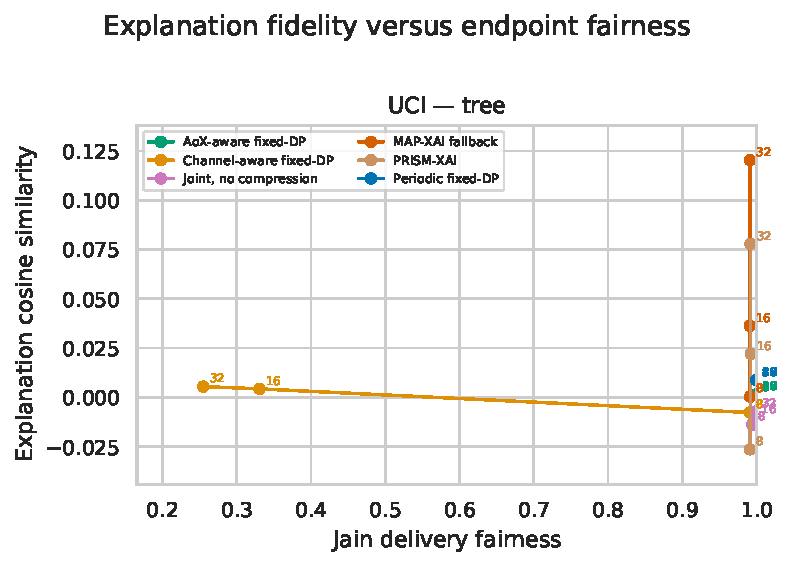
\includegraphics[width=.96\textwidth,height=.82\textheight,keepaspectratio]{../../SERVICE_TRADEOFF_RESULTS/runs/thr_1_cap_8/uci/fairness_reliability.pdf}

\caption{Public-score threshold $\tau=1$, release cap $M=8$, UCI: fairness--reliability plane. This panel should be read with the setting-level quantitative interpretation and the complete tables immediately preceding the figure block.}

\end{figure*}

\clearpage

\begin{figure*}[p]

\centering

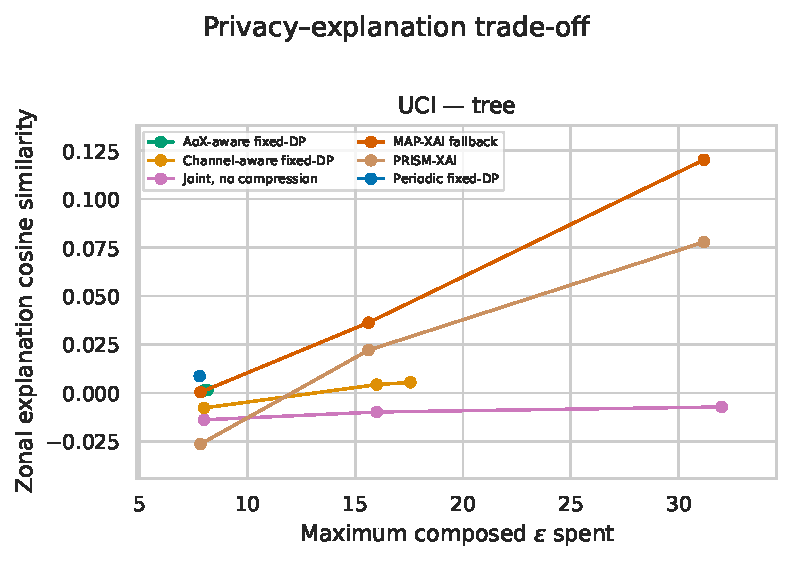
\includegraphics[width=.96\textwidth,height=.82\textheight,keepaspectratio]{../../SERVICE_TRADEOFF_RESULTS/runs/thr_1_cap_8/uci/privacy_fidelity.pdf}

\caption{Public-score threshold $\tau=1$, release cap $M=8$, UCI: privacy--fidelity plane. This panel should be read with the setting-level quantitative interpretation and the complete tables immediately preceding the figure block.}

\end{figure*}

\clearpage

\begin{figure*}[p]

\centering

\includegraphics[width=.96\textwidth,height=.82\textheight,keepaspectratio]{../../SERVICE_TRADEOFF_RESULTS/runs/thr_1_cap_8/uci/pareto_bits_fidelity.pdf}

\caption{Public-score threshold $\tau=1$, release cap $M=8$, UCI: traffic--fidelity Pareto plane. This panel should be read with the setting-level quantitative interpretation and the complete tables immediately preceding the figure block.}

\end{figure*}

\clearpage

\begin{figure*}[p]

\centering

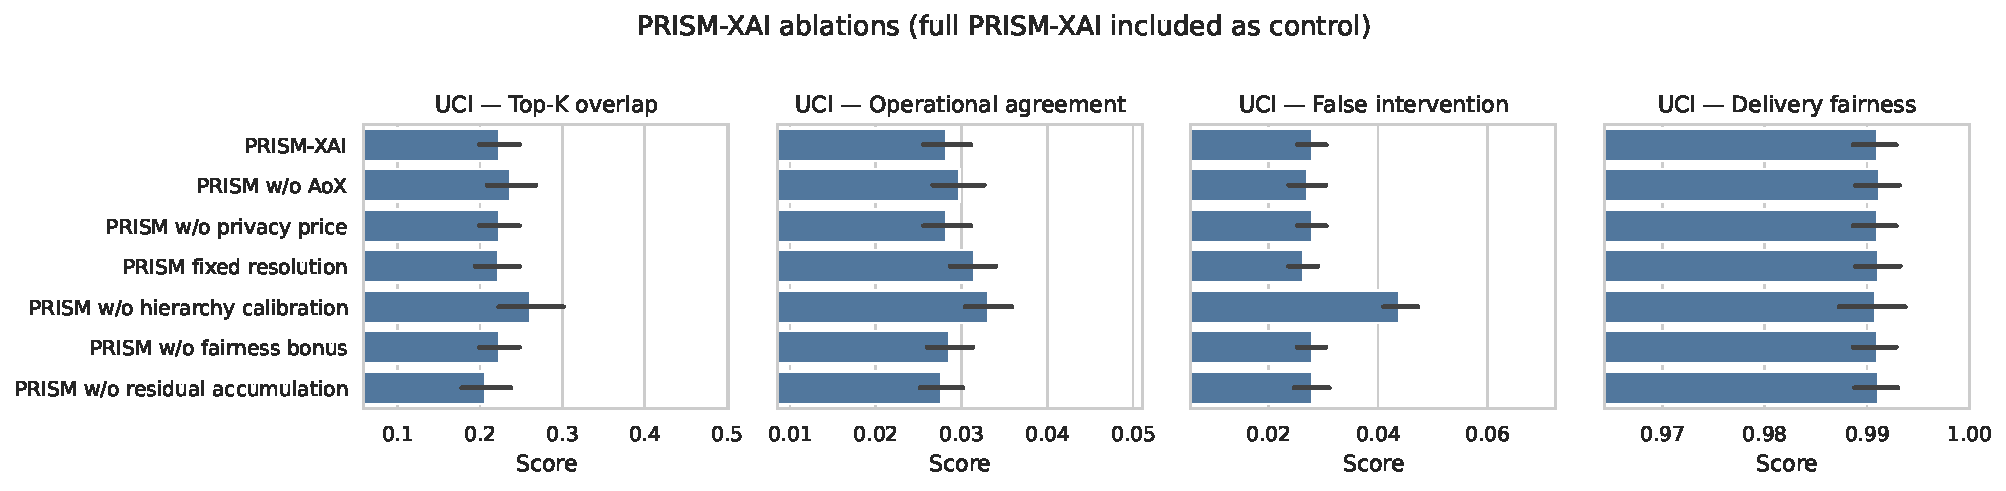
\includegraphics[width=.96\textwidth,height=.82\textheight,keepaspectratio]{../../SERVICE_TRADEOFF_RESULTS/runs/thr_1_cap_8/uci/ablation_results.pdf}

\caption{Public-score threshold $\tau=1$, release cap $M=8$, UCI: component ablation. This panel should be read with the setting-level quantitative interpretation and the complete tables immediately preceding the figure block.}

\end{figure*}

\clearpage

\subsubsection{Public-score threshold $\tau=2$, release cap $M=8$}

At this operating point, PRISM-XAI transmits 205.41~kbit versus 243.37~kbit for MAP-XAI-only (aggregate-mean ratio saving 15.60\%). The paired difference is -37.96$\pm$3.63~kbit. PRISM coverage is 0.0737, critical-event recall is 0.0367, and maximum recorded expenditure is 18.206. Relative to MAP-XAI-only, the paired coverage change is -0.00053$\pm$0.00046 and recall change is -0.00061$\pm$0.00143. The descriptive overlap rule holds in 12 of 12 cells. Accordingly, this point is read as a matched-service scheduler comparison.

\paragraph{Combined datasets.} The three generated tables below report the full method means, all condition-level values, and paired differences. The five figures that follow provide the corresponding temporal, fairness, privacy, Pareto, and ablation views. Aggregate panels support the setting-level summary above; dataset panels reveal whether that summary is shared by OPSD and UCI rather than being driven by their different endpoint counts.

\begin{table*}[p]\centering\tiny

\caption{Public-score threshold $\tau=2$, release cap $M=8$, Combined datasets: complete generated method table.}

\label{tab:thr_2_cap_8:combined:main}

\resizebox{\linewidth}{!}{% Values are means with 95% Student-t confidence intervals across seeds.
\begin{tabular}{lccccccccccccccc}
\toprule
Dataset & Model & $\epsilon_{\max}$ & Method & Top-$K$ & Cosine & Decision & Recall & Prec. & Abst. & P95 ms & kbit & Spent $\epsilon$ & False int. & bit/correct & Fairness \\
\midrule
OPSD & Tree & 8 & AoX-aware fixed-DP & 0.234 $\pm$ 0.048 & -0.033 $\pm$ 0.028 & 0.119 $\pm$ 0.028 & 0.119 $\pm$ 0.028 & 0.198 $\pm$ 0.054 & 0.721 $\pm$ 0.005 & 6.903 $\pm$ 1.126 & 1560.564 $\pm$ 0.000 & 7.990 $\pm$ 0.000 & 0.183 $\pm$ 0.020 & 35567.482 $\pm$ 10569.818 & 0.999 $\pm$ 0.000 \\
OPSD & Tree & 8 & AoX-aware fixed-DP & 0.238 $\pm$ 0.049 & -0.026 $\pm$ 0.055 & 0.121 $\pm$ 0.026 & 0.121 $\pm$ 0.026 & 0.205 $\pm$ 0.053 & 0.721 $\pm$ 0.005 & 6.903 $\pm$ 1.126 & 1560.564 $\pm$ 0.000 & 7.990 $\pm$ 0.000 & 0.179 $\pm$ 0.023 & 34123.214 $\pm$ 8376.542 & 0.999 $\pm$ 0.000 \\
OPSD & Tree & 8 & Channel-aware fixed-DP & 0.292 $\pm$ 0.037 & -0.041 $\pm$ 0.051 & 0.107 $\pm$ 0.026 & 0.107 $\pm$ 0.026 & 0.217 $\pm$ 0.068 & 0.779 $\pm$ 0.011 & 5.571 $\pm$ 1.784 & 1560.564 $\pm$ 0.000 & 7.990 $\pm$ 0.000 & 0.154 $\pm$ 0.029 & 40860.756 $\pm$ 14126.920 & 0.999 $\pm$ 0.000 \\
OPSD & Tree & 8 & Channel-aware fixed-DP & 0.292 $\pm$ 0.054 & -0.049 $\pm$ 0.064 & 0.111 $\pm$ 0.023 & 0.111 $\pm$ 0.023 & 0.228 $\pm$ 0.066 & 0.779 $\pm$ 0.011 & 5.571 $\pm$ 1.784 & 1560.564 $\pm$ 0.000 & 7.990 $\pm$ 0.000 & 0.149 $\pm$ 0.026 & 37980.855 $\pm$ 12338.094 & 0.999 $\pm$ 0.000 \\
OPSD & Tree & 8 & Joint, no compression & 0.288 $\pm$ 0.064 & -0.030 $\pm$ 0.079 & 0.016 $\pm$ 0.005 & 0.016 $\pm$ 0.005 & 0.193 $\pm$ 0.059 & 0.957 $\pm$ 0.003 & 4.560 $\pm$ 1.811 & 189.900 $\pm$ 0.554 & 7.990 $\pm$ 0.000 & 0.027 $\pm$ 0.005 & 32490.357 $\pm$ 10149.755 & 0.996 $\pm$ 0.002 \\
OPSD & Tree & 8 & Joint, no compression & 0.258 $\pm$ 0.055 & 0.011 $\pm$ 0.094 & 0.019 $\pm$ 0.004 & 0.019 $\pm$ 0.004 & 0.224 $\pm$ 0.044 & 0.957 $\pm$ 0.003 & 4.562 $\pm$ 1.809 & 189.750 $\pm$ 0.566 & 7.990 $\pm$ 0.000 & 0.025 $\pm$ 0.003 & 26079.167 $\pm$ 6335.386 & 0.996 $\pm$ 0.002 \\
OPSD & Tree & 8 & Periodic fixed-DP & 0.241 $\pm$ 0.049 & -0.019 $\pm$ 0.061 & 0.125 $\pm$ 0.020 & 0.125 $\pm$ 0.020 & 0.209 $\pm$ 0.044 & 0.722 $\pm$ 0.006 & 6.303 $\pm$ 1.438 & 1560.564 $\pm$ 0.000 & 7.990 $\pm$ 0.000 & 0.181 $\pm$ 0.021 & 31183.082 $\pm$ 4356.378 & 0.999 $\pm$ 0.000 \\
OPSD & Tree & 8 & Periodic fixed-DP & 0.242 $\pm$ 0.048 & -0.026 $\pm$ 0.082 & 0.135 $\pm$ 0.016 & 0.135 $\pm$ 0.016 & 0.231 $\pm$ 0.037 & 0.722 $\pm$ 0.006 & 6.303 $\pm$ 1.438 & 1560.564 $\pm$ 0.000 & 7.990 $\pm$ 0.000 & 0.169 $\pm$ 0.017 & 28520.235 $\pm$ 3511.595 & 0.999 $\pm$ 0.000 \\
OPSD & Tree & 8 & PRISM-XAI & 0.181 $\pm$ 0.038 & 0.036 $\pm$ 0.059 & 0.031 $\pm$ 0.010 & 0.031 $\pm$ 0.010 & 0.347 $\pm$ 0.128 & 0.938 $\pm$ 0.004 & 4.881 $\pm$ 1.730 & 87.922 $\pm$ 0.587 & 7.823 $\pm$ 0.000 & 0.023 $\pm$ 0.007 & 8276.543 $\pm$ 2832.262 & 0.991 $\pm$ 0.006 \\
OPSD & Tree & 8 & PRISM-XAI & 0.204 $\pm$ 0.062 & 0.043 $\pm$ 0.077 & 0.029 $\pm$ 0.009 & 0.029 $\pm$ 0.009 & 0.330 $\pm$ 0.128 & 0.938 $\pm$ 0.004 & 4.876 $\pm$ 1.737 & 87.707 $\pm$ 0.512 & 7.823 $\pm$ 0.000 & 0.025 $\pm$ 0.007 & 8335.040 $\pm$ 2320.748 & 0.991 $\pm$ 0.006 \\
OPSD & Tree & 8 & MAP-XAI fallback & 0.221 $\pm$ 0.065 & 0.030 $\pm$ 0.075 & 0.029 $\pm$ 0.009 & 0.029 $\pm$ 0.009 & 0.319 $\pm$ 0.121 & 0.938 $\pm$ 0.004 & 4.960 $\pm$ 1.678 & 105.889 $\pm$ 0.169 & 7.823 $\pm$ 0.000 & 0.024 $\pm$ 0.006 & 10646.987 $\pm$ 3613.342 & 0.991 $\pm$ 0.006 \\
OPSD & Tree & 8 & MAP-XAI fallback & 0.192 $\pm$ 0.066 & 0.031 $\pm$ 0.076 & 0.027 $\pm$ 0.007 & 0.027 $\pm$ 0.007 & 0.297 $\pm$ 0.095 & 0.938 $\pm$ 0.004 & 4.960 $\pm$ 1.678 & 105.737 $\pm$ 0.152 & 7.823 $\pm$ 0.000 & 0.026 $\pm$ 0.006 & 10712.923 $\pm$ 2768.192 & 0.991 $\pm$ 0.006 \\
UCI & Tree & 8 & AoX-aware fixed-DP & 0.263 $\pm$ 0.041 & -0.007 $\pm$ 0.009 & 0.457 $\pm$ 0.031 & 0.457 $\pm$ 0.031 & 0.362 $\pm$ 0.024 & 0.003 $\pm$ 0.001 & 7.500 $\pm$ 0.000 & 5300.224 $\pm$ 0.000 & 7.990 $\pm$ 0.000 & 0.557 $\pm$ 0.025 & 14002.896 $\pm$ 1040.243 & 0.999 $\pm$ 0.000 \\
UCI & Tree & 8 & AoX-aware fixed-DP & 0.260 $\pm$ 0.022 & 0.010 $\pm$ 0.055 & 0.455 $\pm$ 0.047 & 0.455 $\pm$ 0.047 & 0.361 $\pm$ 0.038 & 0.003 $\pm$ 0.001 & 7.500 $\pm$ 0.000 & 5300.224 $\pm$ 0.000 & 7.990 $\pm$ 0.000 & 0.557 $\pm$ 0.048 & 14198.303 $\pm$ 1508.274 & 0.999 $\pm$ 0.000 \\
UCI & Tree & 8 & Channel-aware fixed-DP & 0.248 $\pm$ 0.031 & 0.004 $\pm$ 0.012 & 0.001 $\pm$ 0.001 & 0.001 $\pm$ 0.001 & 0.150 $\pm$ 0.151 & 0.999 $\pm$ 0.001 & 4.609 $\pm$ 1.781 & 5295.177 $\pm$ 3.740 & 7.990 $\pm$ 0.000 & 0.001 $\pm$ 0.001 & 4632196.500 $\pm$ 2102650.252 & 0.991 $\pm$ 0.001 \\
UCI & Tree & 8 & Channel-aware fixed-DP & 0.239 $\pm$ 0.030 & -0.020 $\pm$ 0.055 & 0.000 $\pm$ 0.000 & 0.000 $\pm$ 0.000 & 0.117 $\pm$ 0.225 & 0.999 $\pm$ 0.001 & 4.609 $\pm$ 1.781 & 5295.177 $\pm$ 3.740 & 7.990 $\pm$ 0.000 & 0.001 $\pm$ 0.001 & 5296989.000 $\pm$ 41104.572 & 0.991 $\pm$ 0.001 \\
UCI & Tree & 8 & Joint, no compression & 0.286 $\pm$ 0.045 & 0.004 $\pm$ 0.020 & 0.052 $\pm$ 0.005 & 0.052 $\pm$ 0.005 & 0.406 $\pm$ 0.037 & 0.875 $\pm$ 0.003 & 5.123 $\pm$ 1.792 & 672.300 $\pm$ 0.452 & 7.990 $\pm$ 0.000 & 0.053 $\pm$ 0.004 & 15676.175 $\pm$ 1475.621 & 0.994 $\pm$ 0.003 \\
UCI & Tree & 8 & Joint, no compression & 0.229 $\pm$ 0.052 & -0.032 $\pm$ 0.050 & 0.057 $\pm$ 0.007 & 0.057 $\pm$ 0.007 & 0.428 $\pm$ 0.041 & 0.875 $\pm$ 0.003 & 5.131 $\pm$ 1.787 & 672.300 $\pm$ 0.452 & 7.990 $\pm$ 0.000 & 0.052 $\pm$ 0.004 & 14702.786 $\pm$ 2334.488 & 0.994 $\pm$ 0.003 \\
UCI & Tree & 8 & Periodic fixed-DP & 0.259 $\pm$ 0.060 & -0.005 $\pm$ 0.008 & 0.006 $\pm$ 0.001 & 0.006 $\pm$ 0.001 & 0.244 $\pm$ 0.049 & 0.989 $\pm$ 0.001 & 4.596 $\pm$ 1.788 & 5299.318 $\pm$ 1.451 & 7.786 $\pm$ 0.000 & 0.013 $\pm$ 0.002 & 1215103.896 $\pm$ 390671.319 & 0.999 $\pm$ 0.000 \\
UCI & Tree & 8 & Periodic fixed-DP & 0.260 $\pm$ 0.044 & 0.022 $\pm$ 0.070 & 0.005 $\pm$ 0.001 & 0.005 $\pm$ 0.001 & 0.195 $\pm$ 0.050 & 0.989 $\pm$ 0.001 & 4.596 $\pm$ 1.788 & 5299.318 $\pm$ 1.451 & 7.786 $\pm$ 0.000 & 0.015 $\pm$ 0.002 & 1555837.203 $\pm$ 955472.503 & 0.999 $\pm$ 0.000 \\
UCI & Tree & 8 & PRISM-XAI & 0.226 $\pm$ 0.039 & -0.007 $\pm$ 0.014 & 0.045 $\pm$ 0.006 & 0.045 $\pm$ 0.006 & 0.448 $\pm$ 0.069 & 0.907 $\pm$ 0.003 & 4.627 $\pm$ 1.490 & 325.204 $\pm$ 1.099 & 7.823 $\pm$ 0.000 & 0.038 $\pm$ 0.006 & 9052.203 $\pm$ 1462.054 & 0.991 $\pm$ 0.002 \\
UCI & Tree & 8 & PRISM-XAI & 0.218 $\pm$ 0.040 & -0.021 $\pm$ 0.077 & 0.041 $\pm$ 0.008 & 0.041 $\pm$ 0.008 & 0.442 $\pm$ 0.091 & 0.912 $\pm$ 0.003 & 4.663 $\pm$ 1.766 & 322.006 $\pm$ 0.783 & 7.823 $\pm$ 0.000 & 0.036 $\pm$ 0.008 & 10546.447 $\pm$ 3413.298 & 0.991 $\pm$ 0.003 \\
UCI & Tree & 8 & MAP-XAI fallback & 0.167 $\pm$ 0.072 & -0.002 $\pm$ 0.015 & 0.047 $\pm$ 0.007 & 0.047 $\pm$ 0.007 & 0.444 $\pm$ 0.055 & 0.907 $\pm$ 0.003 & 4.955 $\pm$ 1.626 & 381.383 $\pm$ 0.421 & 7.823 $\pm$ 0.000 & 0.040 $\pm$ 0.005 & 10267.244 $\pm$ 1941.397 & 0.991 $\pm$ 0.002 \\
UCI & Tree & 8 & MAP-XAI fallback & 0.241 $\pm$ 0.074 & 0.039 $\pm$ 0.065 & 0.046 $\pm$ 0.006 & 0.046 $\pm$ 0.006 & 0.475 $\pm$ 0.053 & 0.909 $\pm$ 0.003 & 5.078 $\pm$ 1.827 & 381.010 $\pm$ 0.445 & 7.823 $\pm$ 0.000 & 0.035 $\pm$ 0.005 & 10274.502 $\pm$ 1367.610 & 0.991 $\pm$ 0.003 \\
\bottomrule
\end{tabular}
}

\end{table*}\clearpage

\begin{table*}[p]\centering\tiny

\caption{Public-score threshold $\tau=2$, release cap $M=8$, Combined datasets: complete condition-level generated table.}

\label{tab:thr_2_cap_8:combined:conditions}

\resizebox{\textwidth}{!}{\begin{tabular}{llllccccccccccc}
\toprule
Dataset & Model & $\epsilon_{\max}$ & Method & kbit & Top-$K$ & Random Top-$K$ & Cosine & Decision & Recall & Precision & Coverage & Abstain & False int. & Spent $\epsilon$ \\
\midrule
OPSD & Tree & 8 & Joint, no compression & 189.900 $\pm$ 0.554 & 0.288 $\pm$ 0.064 & 0.250 $\pm$ 0.000 & -0.030 $\pm$ 0.079 & 0.016 $\pm$ 0.005 & 0.016 $\pm$ 0.005 & 0.193 $\pm$ 0.059 & 0.043 $\pm$ 0.003 & 0.957 $\pm$ 0.003 & 0.027 $\pm$ 0.005 & 7.990 $\pm$ 0.000 \\
OPSD & Tree & 8 & Joint, no compression & 189.750 $\pm$ 0.566 & 0.258 $\pm$ 0.055 & 0.250 $\pm$ 0.000 & 0.011 $\pm$ 0.094 & 0.019 $\pm$ 0.004 & 0.019 $\pm$ 0.004 & 0.224 $\pm$ 0.044 & 0.043 $\pm$ 0.003 & 0.957 $\pm$ 0.003 & 0.025 $\pm$ 0.003 & 7.990 $\pm$ 0.000 \\
OPSD & Tree & 8 & Periodic fixed-DP & 1560.564 $\pm$ 0.000 & 0.241 $\pm$ 0.049 & 0.250 $\pm$ 0.000 & -0.019 $\pm$ 0.061 & 0.125 $\pm$ 0.020 & 0.125 $\pm$ 0.020 & 0.209 $\pm$ 0.044 & 0.278 $\pm$ 0.006 & 0.722 $\pm$ 0.006 & 0.181 $\pm$ 0.021 & 7.990 $\pm$ 0.000 \\
OPSD & Tree & 8 & Periodic fixed-DP & 1560.564 $\pm$ 0.000 & 0.242 $\pm$ 0.048 & 0.250 $\pm$ 0.000 & -0.026 $\pm$ 0.082 & 0.135 $\pm$ 0.016 & 0.135 $\pm$ 0.016 & 0.231 $\pm$ 0.037 & 0.278 $\pm$ 0.006 & 0.722 $\pm$ 0.006 & 0.169 $\pm$ 0.017 & 7.990 $\pm$ 0.000 \\
OPSD & Tree & 8 & PRISM-XAI & 87.922 $\pm$ 0.587 & 0.181 $\pm$ 0.038 & 0.250 $\pm$ 0.000 & 0.036 $\pm$ 0.059 & 0.031 $\pm$ 0.010 & 0.031 $\pm$ 0.010 & 0.347 $\pm$ 0.128 & 0.062 $\pm$ 0.004 & 0.938 $\pm$ 0.004 & 0.023 $\pm$ 0.007 & 7.823 $\pm$ 0.000 \\
OPSD & Tree & 8 & PRISM-XAI & 87.707 $\pm$ 0.512 & 0.204 $\pm$ 0.062 & 0.250 $\pm$ 0.000 & 0.043 $\pm$ 0.077 & 0.029 $\pm$ 0.009 & 0.029 $\pm$ 0.009 & 0.330 $\pm$ 0.128 & 0.062 $\pm$ 0.004 & 0.938 $\pm$ 0.004 & 0.025 $\pm$ 0.007 & 7.823 $\pm$ 0.000 \\
OPSD & Tree & 16 & Joint, no compression & 459.900 $\pm$ 0.750 & 0.232 $\pm$ 0.065 & 0.250 $\pm$ 0.000 & 0.059 $\pm$ 0.048 & 0.038 $\pm$ 0.009 & 0.038 $\pm$ 0.009 & 0.222 $\pm$ 0.049 & 0.088 $\pm$ 0.004 & 0.912 $\pm$ 0.004 & 0.049 $\pm$ 0.005 & 15.997 $\pm$ 0.000 \\
OPSD & Tree & 16 & Joint, no compression & 460.050 $\pm$ 0.724 & 0.241 $\pm$ 0.055 & 0.250 $\pm$ 0.000 & 0.061 $\pm$ 0.052 & 0.039 $\pm$ 0.008 & 0.039 $\pm$ 0.008 & 0.241 $\pm$ 0.042 & 0.088 $\pm$ 0.004 & 0.912 $\pm$ 0.004 & 0.045 $\pm$ 0.004 & 15.997 $\pm$ 0.000 \\
OPSD & Tree & 16 & Periodic fixed-DP & 5112.594 $\pm$ 0.000 & 0.249 $\pm$ 0.022 & 0.250 $\pm$ 0.000 & -0.009 $\pm$ 0.045 & 0.450 $\pm$ 0.062 & 0.450 $\pm$ 0.062 & 0.237 $\pm$ 0.042 & 0.985 $\pm$ 0.002 & 0.015 $\pm$ 0.002 & 0.551 $\pm$ 0.057 & 15.997 $\pm$ 0.000 \\
OPSD & Tree & 16 & Periodic fixed-DP & 5112.594 $\pm$ 0.000 & 0.243 $\pm$ 0.019 & 0.250 $\pm$ 0.000 & -0.012 $\pm$ 0.050 & 0.463 $\pm$ 0.047 & 0.463 $\pm$ 0.047 & 0.240 $\pm$ 0.028 & 0.985 $\pm$ 0.002 & 0.015 $\pm$ 0.002 & 0.547 $\pm$ 0.036 & 15.997 $\pm$ 0.000 \\
OPSD & Tree & 16 & PRISM-XAI & 87.922 $\pm$ 0.597 & 0.221 $\pm$ 0.066 & 0.250 $\pm$ 0.000 & 0.141 $\pm$ 0.056 & 0.029 $\pm$ 0.010 & 0.029 $\pm$ 0.010 & 0.385 $\pm$ 0.148 & 0.062 $\pm$ 0.004 & 0.938 $\pm$ 0.004 & 0.020 $\pm$ 0.007 & 15.620 $\pm$ 0.000 \\
OPSD & Tree & 16 & PRISM-XAI & 87.585 $\pm$ 0.454 & 0.246 $\pm$ 0.046 & 0.250 $\pm$ 0.000 & 0.149 $\pm$ 0.072 & 0.030 $\pm$ 0.008 & 0.030 $\pm$ 0.008 & 0.354 $\pm$ 0.120 & 0.062 $\pm$ 0.004 & 0.938 $\pm$ 0.004 & 0.022 $\pm$ 0.006 & 15.620 $\pm$ 0.000 \\
OPSD & Tree & 32 & Joint, no compression & 1140.900 $\pm$ 7.953 & 0.235 $\pm$ 0.064 & 0.250 $\pm$ 0.000 & -0.031 $\pm$ 0.089 & 0.074 $\pm$ 0.015 & 0.074 $\pm$ 0.015 & 0.205 $\pm$ 0.039 & 0.157 $\pm$ 0.006 & 0.843 $\pm$ 0.006 & 0.107 $\pm$ 0.009 & 31.999 $\pm$ 0.000 \\
OPSD & Tree & 32 & Joint, no compression & 1140.900 $\pm$ 7.953 & 0.282 $\pm$ 0.054 & 0.250 $\pm$ 0.000 & -0.044 $\pm$ 0.076 & 0.080 $\pm$ 0.011 & 0.080 $\pm$ 0.011 & 0.227 $\pm$ 0.052 & 0.158 $\pm$ 0.006 & 0.842 $\pm$ 0.006 & 0.105 $\pm$ 0.015 & 31.999 $\pm$ 0.000 \\
OPSD & Tree & 32 & Periodic fixed-DP & 5299.836 $\pm$ 0.625 & 0.249 $\pm$ 0.022 & 0.250 $\pm$ 0.000 & -0.009 $\pm$ 0.044 & 0.458 $\pm$ 0.066 & 0.458 $\pm$ 0.066 & 0.237 $\pm$ 0.045 & 1.000 $\pm$ 0.000 & 0.000 $\pm$ 0.000 & 0.562 $\pm$ 0.062 & 16.371 $\pm$ 0.000 \\
OPSD & Tree & 32 & Periodic fixed-DP & 5299.836 $\pm$ 0.625 & 0.244 $\pm$ 0.019 & 0.250 $\pm$ 0.000 & -0.012 $\pm$ 0.050 & 0.471 $\pm$ 0.049 & 0.471 $\pm$ 0.049 & 0.240 $\pm$ 0.029 & 1.000 $\pm$ 0.000 & 0.000 $\pm$ 0.000 & 0.559 $\pm$ 0.039 & 16.371 $\pm$ 0.000 \\
OPSD & Tree & 32 & PRISM-XAI & 87.891 $\pm$ 0.540 & 0.397 $\pm$ 0.067 & 0.250 $\pm$ 0.000 & 0.306 $\pm$ 0.044 & 0.040 $\pm$ 0.008 & 0.040 $\pm$ 0.008 & 0.627 $\pm$ 0.190 & 0.063 $\pm$ 0.004 & 0.937 $\pm$ 0.004 & 0.011 $\pm$ 0.007 & 31.175 $\pm$ 0.000 \\
OPSD & Tree & 32 & PRISM-XAI & 87.431 $\pm$ 0.439 & 0.369 $\pm$ 0.054 & 0.250 $\pm$ 0.000 & 0.347 $\pm$ 0.057 & 0.041 $\pm$ 0.006 & 0.041 $\pm$ 0.006 & 0.574 $\pm$ 0.099 & 0.062 $\pm$ 0.004 & 0.938 $\pm$ 0.004 & 0.012 $\pm$ 0.004 & 31.175 $\pm$ 0.000 \\
UCI & Tree & 8 & Joint, no compression & 672.300 $\pm$ 0.452 & 0.286 $\pm$ 0.045 & 0.250 $\pm$ 0.000 & 0.004 $\pm$ 0.020 & 0.052 $\pm$ 0.005 & 0.052 $\pm$ 0.005 & 0.406 $\pm$ 0.037 & 0.125 $\pm$ 0.003 & 0.875 $\pm$ 0.003 & 0.053 $\pm$ 0.004 & 7.990 $\pm$ 0.000 \\
UCI & Tree & 8 & Joint, no compression & 672.300 $\pm$ 0.452 & 0.229 $\pm$ 0.052 & 0.250 $\pm$ 0.000 & -0.032 $\pm$ 0.050 & 0.057 $\pm$ 0.007 & 0.057 $\pm$ 0.007 & 0.428 $\pm$ 0.041 & 0.125 $\pm$ 0.003 & 0.875 $\pm$ 0.003 & 0.052 $\pm$ 0.004 & 7.990 $\pm$ 0.000 \\
UCI & Tree & 8 & Periodic fixed-DP & 5299.318 $\pm$ 1.451 & 0.259 $\pm$ 0.060 & 0.250 $\pm$ 0.000 & -0.005 $\pm$ 0.008 & 0.006 $\pm$ 0.001 & 0.006 $\pm$ 0.001 & 0.244 $\pm$ 0.049 & 0.011 $\pm$ 0.001 & 0.989 $\pm$ 0.001 & 0.013 $\pm$ 0.002 & 7.786 $\pm$ 0.000 \\
UCI & Tree & 8 & Periodic fixed-DP & 5299.318 $\pm$ 1.451 & 0.260 $\pm$ 0.044 & 0.250 $\pm$ 0.000 & 0.022 $\pm$ 0.070 & 0.005 $\pm$ 0.001 & 0.005 $\pm$ 0.001 & 0.195 $\pm$ 0.050 & 0.011 $\pm$ 0.001 & 0.989 $\pm$ 0.001 & 0.015 $\pm$ 0.002 & 7.786 $\pm$ 0.000 \\
UCI & Tree & 8 & PRISM-XAI & 325.204 $\pm$ 1.099 & 0.226 $\pm$ 0.039 & 0.250 $\pm$ 0.000 & -0.007 $\pm$ 0.014 & 0.045 $\pm$ 0.006 & 0.045 $\pm$ 0.006 & 0.448 $\pm$ 0.069 & 0.093 $\pm$ 0.003 & 0.907 $\pm$ 0.003 & 0.038 $\pm$ 0.006 & 7.823 $\pm$ 0.000 \\
UCI & Tree & 8 & PRISM-XAI & 322.006 $\pm$ 0.783 & 0.218 $\pm$ 0.040 & 0.250 $\pm$ 0.000 & -0.021 $\pm$ 0.077 & 0.041 $\pm$ 0.008 & 0.041 $\pm$ 0.008 & 0.442 $\pm$ 0.091 & 0.088 $\pm$ 0.003 & 0.912 $\pm$ 0.003 & 0.036 $\pm$ 0.008 & 7.823 $\pm$ 0.000 \\
UCI & Tree & 16 & Joint, no compression & 1632.150 $\pm$ 0.339 & 0.216 $\pm$ 0.041 & 0.250 $\pm$ 0.000 & 0.001 $\pm$ 0.012 & 0.094 $\pm$ 0.005 & 0.094 $\pm$ 0.005 & 0.330 $\pm$ 0.024 & 0.228 $\pm$ 0.005 & 0.772 $\pm$ 0.005 & 0.133 $\pm$ 0.010 & 15.997 $\pm$ 0.000 \\
UCI & Tree & 16 & Joint, no compression & 1632.600 $\pm$ 0.554 & 0.204 $\pm$ 0.011 & 0.250 $\pm$ 0.000 & -0.021 $\pm$ 0.033 & 0.099 $\pm$ 0.016 & 0.099 $\pm$ 0.016 & 0.347 $\pm$ 0.054 & 0.228 $\pm$ 0.005 & 0.772 $\pm$ 0.005 & 0.128 $\pm$ 0.011 & 15.997 $\pm$ 0.000 \\
UCI & Tree & 16 & Periodic fixed-DP & 5299.318 $\pm$ 1.451 & 0.259 $\pm$ 0.060 & 0.250 $\pm$ 0.000 & -0.005 $\pm$ 0.008 & 0.006 $\pm$ 0.001 & 0.006 $\pm$ 0.001 & 0.244 $\pm$ 0.049 & 0.011 $\pm$ 0.001 & 0.989 $\pm$ 0.001 & 0.013 $\pm$ 0.002 & 7.786 $\pm$ 0.000 \\
UCI & Tree & 16 & Periodic fixed-DP & 5299.318 $\pm$ 1.451 & 0.260 $\pm$ 0.044 & 0.250 $\pm$ 0.000 & 0.022 $\pm$ 0.070 & 0.005 $\pm$ 0.001 & 0.005 $\pm$ 0.001 & 0.195 $\pm$ 0.050 & 0.011 $\pm$ 0.001 & 0.989 $\pm$ 0.001 & 0.015 $\pm$ 0.002 & 7.786 $\pm$ 0.000 \\
UCI & Tree & 16 & PRISM-XAI & 324.692 $\pm$ 0.734 & 0.260 $\pm$ 0.069 & 0.250 $\pm$ 0.000 & -0.003 $\pm$ 0.016 & 0.041 $\pm$ 0.006 & 0.041 $\pm$ 0.006 & 0.561 $\pm$ 0.104 & 0.090 $\pm$ 0.004 & 0.910 $\pm$ 0.004 & 0.023 $\pm$ 0.006 & 15.620 $\pm$ 0.000 \\
UCI & Tree & 16 & PRISM-XAI & 321.197 $\pm$ 1.037 & 0.247 $\pm$ 0.060 & 0.250 $\pm$ 0.000 & -0.017 $\pm$ 0.061 & 0.038 $\pm$ 0.007 & 0.038 $\pm$ 0.007 & 0.561 $\pm$ 0.070 & 0.081 $\pm$ 0.003 & 0.919 $\pm$ 0.003 & 0.021 $\pm$ 0.004 & 15.620 $\pm$ 0.000 \\
UCI & Tree & 32 & Joint, no compression & 4034.550 $\pm$ 5.034 & 0.246 $\pm$ 0.031 & 0.250 $\pm$ 0.000 & -0.002 $\pm$ 0.015 & 0.228 $\pm$ 0.013 & 0.228 $\pm$ 0.013 & 0.361 $\pm$ 0.028 & 0.537 $\pm$ 0.009 & 0.463 $\pm$ 0.009 & 0.279 $\pm$ 0.017 & 31.999 $\pm$ 0.000 \\
UCI & Tree & 32 & Joint, no compression & 4034.550 $\pm$ 5.034 & 0.241 $\pm$ 0.033 & 0.250 $\pm$ 0.000 & -0.012 $\pm$ 0.030 & 0.228 $\pm$ 0.028 & 0.228 $\pm$ 0.028 & 0.360 $\pm$ 0.047 & 0.530 $\pm$ 0.010 & 0.470 $\pm$ 0.010 & 0.280 $\pm$ 0.026 & 31.999 $\pm$ 0.000 \\
UCI & Tree & 32 & Periodic fixed-DP & 5299.318 $\pm$ 1.451 & 0.259 $\pm$ 0.060 & 0.250 $\pm$ 0.000 & -0.005 $\pm$ 0.008 & 0.006 $\pm$ 0.001 & 0.006 $\pm$ 0.001 & 0.244 $\pm$ 0.049 & 0.011 $\pm$ 0.001 & 0.989 $\pm$ 0.001 & 0.013 $\pm$ 0.002 & 7.786 $\pm$ 0.000 \\
UCI & Tree & 32 & Periodic fixed-DP & 5299.318 $\pm$ 1.451 & 0.260 $\pm$ 0.044 & 0.250 $\pm$ 0.000 & 0.022 $\pm$ 0.070 & 0.005 $\pm$ 0.001 & 0.005 $\pm$ 0.001 & 0.195 $\pm$ 0.050 & 0.011 $\pm$ 0.001 & 0.989 $\pm$ 0.001 & 0.015 $\pm$ 0.002 & 7.786 $\pm$ 0.000 \\
UCI & Tree & 32 & PRISM-XAI & 324.272 $\pm$ 0.853 & 0.285 $\pm$ 0.057 & 0.250 $\pm$ 0.000 & 0.008 $\pm$ 0.016 & 0.039 $\pm$ 0.004 & 0.039 $\pm$ 0.004 & 0.892 $\pm$ 0.052 & 0.081 $\pm$ 0.003 & 0.919 $\pm$ 0.003 & 0.004 $\pm$ 0.002 & 31.175 $\pm$ 0.000 \\
UCI & Tree & 32 & PRISM-XAI & 321.095 $\pm$ 0.887 & 0.246 $\pm$ 0.074 & 0.250 $\pm$ 0.000 & 0.042 $\pm$ 0.069 & 0.036 $\pm$ 0.005 & 0.036 $\pm$ 0.005 & 0.872 $\pm$ 0.111 & 0.076 $\pm$ 0.004 & 0.924 $\pm$ 0.004 & 0.004 $\pm$ 0.004 & 31.175 $\pm$ 0.000 \\
\bottomrule
\end{tabular}
}

\end{table*}\clearpage

\begin{table*}[p]\centering\tiny

\caption{Public-score threshold $\tau=2$, release cap $M=8$, Combined datasets: complete generated paired comparisons.}

\label{tab:thr_2_cap_8:combined:paired}

\resizebox{\textwidth}{!}{\begin{tabular}{llcccc}
\toprule
Dataset & Baseline & Delta kbit & Delta Top-$K$ & Delta recall & Delta fairness \\
\midrule
OPSD & AoX-aware fixed-DP & -1472.642 $\pm$ 0.587 & -0.052 $\pm$ 0.056 & -0.089 $\pm$ 0.033 & -0.008 $\pm$ 0.006 \\
OPSD & AoX-aware fixed-DP & -5011.991 $\pm$ 5.546 & -0.033 $\pm$ 0.086 & -0.372 $\pm$ 0.079 & -0.009 $\pm$ 0.006 \\
OPSD & AoX-aware fixed-DP & -5212.333 $\pm$ 0.540 & 0.144 $\pm$ 0.080 & -0.373 $\pm$ 0.080 & -0.009 $\pm$ 0.006 \\
OPSD & AoX-aware fixed-DP & -1472.857 $\pm$ 0.512 & -0.034 $\pm$ 0.064 & -0.091 $\pm$ 0.028 & -0.008 $\pm$ 0.006 \\
OPSD & AoX-aware fixed-DP & -5012.328 $\pm$ 5.478 & -0.006 $\pm$ 0.062 & -0.385 $\pm$ 0.059 & -0.009 $\pm$ 0.006 \\
OPSD & AoX-aware fixed-DP & -5212.793 $\pm$ 0.439 & 0.117 $\pm$ 0.064 & -0.384 $\pm$ 0.059 & -0.008 $\pm$ 0.006 \\
OPSD & Channel-aware fixed-DP & -1472.642 $\pm$ 0.587 & -0.111 $\pm$ 0.049 & -0.076 $\pm$ 0.029 & -0.008 $\pm$ 0.006 \\
OPSD & Channel-aware fixed-DP & -4598.687 $\pm$ 12.788 & -0.041 $\pm$ 0.083 & -0.372 $\pm$ 0.091 & 0.054 $\pm$ 0.008 \\
OPSD & Channel-aware fixed-DP & -5212.333 $\pm$ 0.540 & 0.139 $\pm$ 0.074 & -0.394 $\pm$ 0.099 & 0.083 $\pm$ 0.008 \\
OPSD & Channel-aware fixed-DP & -1472.857 $\pm$ 0.512 & -0.088 $\pm$ 0.072 & -0.082 $\pm$ 0.026 & -0.008 $\pm$ 0.006 \\
OPSD & Channel-aware fixed-DP & -4599.025 $\pm$ 12.782 & -0.012 $\pm$ 0.057 & -0.389 $\pm$ 0.089 & 0.054 $\pm$ 0.008 \\
OPSD & Channel-aware fixed-DP & -5212.793 $\pm$ 0.439 & 0.112 $\pm$ 0.064 & -0.415 $\pm$ 0.091 & 0.085 $\pm$ 0.008 \\
OPSD & Joint, no compression & -101.978 $\pm$ 0.649 & -0.106 $\pm$ 0.082 & 0.014 $\pm$ 0.009 & -0.005 $\pm$ 0.005 \\
OPSD & Joint, no compression & -371.978 $\pm$ 1.235 & -0.011 $\pm$ 0.086 & -0.009 $\pm$ 0.014 & -0.006 $\pm$ 0.006 \\
OPSD & Joint, no compression & -1053.008 $\pm$ 7.902 & 0.162 $\pm$ 0.100 & -0.034 $\pm$ 0.017 & -0.009 $\pm$ 0.006 \\
OPSD & Joint, no compression & -102.043 $\pm$ 0.542 & -0.054 $\pm$ 0.092 & 0.010 $\pm$ 0.008 & -0.005 $\pm$ 0.005 \\
OPSD & Joint, no compression & -372.466 $\pm$ 0.983 & 0.006 $\pm$ 0.073 & -0.009 $\pm$ 0.011 & -0.006 $\pm$ 0.006 \\
OPSD & Joint, no compression & -1053.469 $\pm$ 8.014 & 0.087 $\pm$ 0.081 & -0.039 $\pm$ 0.013 & -0.007 $\pm$ 0.006 \\
OPSD & Periodic fixed-DP & -1472.642 $\pm$ 0.587 & -0.059 $\pm$ 0.047 & -0.094 $\pm$ 0.024 & -0.008 $\pm$ 0.006 \\
OPSD & Periodic fixed-DP & -5024.672 $\pm$ 0.597 & -0.028 $\pm$ 0.077 & -0.421 $\pm$ 0.066 & -0.009 $\pm$ 0.006 \\
OPSD & Periodic fixed-DP & -5211.944 $\pm$ 0.546 & 0.148 $\pm$ 0.067 & -0.418 $\pm$ 0.066 & -0.010 $\pm$ 0.006 \\
OPSD & Periodic fixed-DP & -1472.857 $\pm$ 0.512 & -0.038 $\pm$ 0.054 & -0.105 $\pm$ 0.018 & -0.008 $\pm$ 0.006 \\
OPSD & Periodic fixed-DP & -5025.010 $\pm$ 0.454 & 0.003 $\pm$ 0.052 & -0.433 $\pm$ 0.050 & -0.009 $\pm$ 0.006 \\
OPSD & Periodic fixed-DP & -5212.405 $\pm$ 0.471 & 0.125 $\pm$ 0.063 & -0.430 $\pm$ 0.050 & -0.009 $\pm$ 0.006 \\
OPSD & MAP-XAI fallback & -17.966 $\pm$ 0.682 & -0.040 $\pm$ 0.046 & 0.002 $\pm$ 0.004 & 0.000 $\pm$ 0.000 \\
OPSD & MAP-XAI fallback & -17.966 $\pm$ 0.687 & -0.043 $\pm$ 0.089 & 0.000 $\pm$ 0.006 & 0.000 $\pm$ 0.000 \\
OPSD & MAP-XAI fallback & -17.997 $\pm$ 0.643 & -0.000 $\pm$ 0.067 & -0.002 $\pm$ 0.005 & -0.001 $\pm$ 0.003 \\
OPSD & MAP-XAI fallback & -18.030 $\pm$ 0.583 & 0.013 $\pm$ 0.040 & 0.003 $\pm$ 0.006 & 0.000 $\pm$ 0.000 \\
OPSD & MAP-XAI fallback & -18.153 $\pm$ 0.544 & 0.003 $\pm$ 0.052 & 0.002 $\pm$ 0.005 & 0.000 $\pm$ 0.000 \\
OPSD & MAP-XAI fallback & -18.121 $\pm$ 0.487 & 0.009 $\pm$ 0.066 & 0.004 $\pm$ 0.005 & 0.000 $\pm$ 0.000 \\
UCI & AoX-aware fixed-DP & -4975.020 $\pm$ 1.099 & -0.037 $\pm$ 0.046 & -0.412 $\pm$ 0.033 & -0.008 $\pm$ 0.002 \\
UCI & AoX-aware fixed-DP & -4975.532 $\pm$ 0.734 & -0.003 $\pm$ 0.089 & -0.416 $\pm$ 0.028 & -0.007 $\pm$ 0.003 \\
UCI & AoX-aware fixed-DP & -4975.952 $\pm$ 0.853 & 0.021 $\pm$ 0.068 & -0.418 $\pm$ 0.031 & -0.007 $\pm$ 0.002 \\
UCI & AoX-aware fixed-DP & -4978.218 $\pm$ 0.783 & -0.043 $\pm$ 0.038 & -0.414 $\pm$ 0.047 & -0.009 $\pm$ 0.003 \\
UCI & AoX-aware fixed-DP & -4979.027 $\pm$ 1.037 & -0.013 $\pm$ 0.061 & -0.416 $\pm$ 0.044 & -0.007 $\pm$ 0.002 \\
UCI & AoX-aware fixed-DP & -4979.130 $\pm$ 0.887 & -0.014 $\pm$ 0.081 & -0.419 $\pm$ 0.045 & -0.008 $\pm$ 0.002 \\
UCI & Channel-aware fixed-DP & -4969.974 $\pm$ 3.637 & -0.022 $\pm$ 0.056 & 0.044 $\pm$ 0.006 & 0.001 $\pm$ 0.002 \\
UCI & Channel-aware fixed-DP & -4975.532 $\pm$ 0.734 & -0.007 $\pm$ 0.079 & 0.040 $\pm$ 0.006 & 0.661 $\pm$ 0.003 \\
UCI & Channel-aware fixed-DP & -4975.952 $\pm$ 0.853 & 0.016 $\pm$ 0.078 & 0.039 $\pm$ 0.004 & 0.737 $\pm$ 0.002 \\
UCI & Channel-aware fixed-DP & -4973.172 $\pm$ 3.993 & -0.022 $\pm$ 0.051 & 0.041 $\pm$ 0.008 & -0.000 $\pm$ 0.003 \\
UCI & Channel-aware fixed-DP & -4979.027 $\pm$ 1.037 & -0.013 $\pm$ 0.056 & 0.038 $\pm$ 0.007 & 0.661 $\pm$ 0.002 \\
UCI & Channel-aware fixed-DP & -4979.130 $\pm$ 0.887 & -0.013 $\pm$ 0.077 & 0.035 $\pm$ 0.005 & 0.736 $\pm$ 0.002 \\
UCI & Joint, no compression & -347.096 $\pm$ 1.294 & -0.060 $\pm$ 0.070 & -0.007 $\pm$ 0.008 & -0.002 $\pm$ 0.003 \\
UCI & Joint, no compression & -1307.458 $\pm$ 0.943 & 0.044 $\pm$ 0.088 & -0.053 $\pm$ 0.006 & -0.006 $\pm$ 0.002 \\
UCI & Joint, no compression & -3710.278 $\pm$ 4.537 & 0.038 $\pm$ 0.072 & -0.188 $\pm$ 0.014 & -0.007 $\pm$ 0.002 \\
UCI & Joint, no compression & -350.294 $\pm$ 0.927 & -0.012 $\pm$ 0.080 & -0.016 $\pm$ 0.011 & -0.004 $\pm$ 0.004 \\
UCI & Joint, no compression & -1311.403 $\pm$ 0.582 & 0.044 $\pm$ 0.058 & -0.061 $\pm$ 0.019 & -0.006 $\pm$ 0.002 \\
UCI & Joint, no compression & -3713.455 $\pm$ 5.127 & 0.005 $\pm$ 0.053 & -0.192 $\pm$ 0.027 & -0.007 $\pm$ 0.002 \\
UCI & Periodic fixed-DP & -4974.114 $\pm$ 1.995 & -0.033 $\pm$ 0.077 & 0.039 $\pm$ 0.007 & -0.008 $\pm$ 0.002 \\
UCI & Periodic fixed-DP & -4974.626 $\pm$ 1.848 & 0.001 $\pm$ 0.099 & 0.035 $\pm$ 0.007 & -0.008 $\pm$ 0.003 \\
UCI & Periodic fixed-DP & -4975.046 $\pm$ 1.596 & 0.025 $\pm$ 0.092 & 0.033 $\pm$ 0.005 & -0.008 $\pm$ 0.002 \\
UCI & Periodic fixed-DP & -4977.312 $\pm$ 1.437 & -0.043 $\pm$ 0.073 & 0.036 $\pm$ 0.007 & -0.009 $\pm$ 0.003 \\
UCI & Periodic fixed-DP & -4978.121 $\pm$ 1.405 & -0.013 $\pm$ 0.077 & 0.033 $\pm$ 0.007 & -0.007 $\pm$ 0.002 \\
UCI & Periodic fixed-DP & -4978.224 $\pm$ 1.527 & -0.014 $\pm$ 0.101 & 0.030 $\pm$ 0.005 & -0.008 $\pm$ 0.002 \\
UCI & MAP-XAI fallback & -56.179 $\pm$ 0.880 & 0.059 $\pm$ 0.050 & -0.002 $\pm$ 0.004 & 0.000 $\pm$ 0.000 \\
UCI & MAP-XAI fallback & -56.609 $\pm$ 0.650 & 0.023 $\pm$ 0.053 & -0.001 $\pm$ 0.006 & 0.000 $\pm$ 0.001 \\
UCI & MAP-XAI fallback & -56.864 $\pm$ 0.771 & 0.066 $\pm$ 0.045 & -0.003 $\pm$ 0.005 & -0.000 $\pm$ 0.001 \\
UCI & MAP-XAI fallback & -59.004 $\pm$ 0.825 & -0.024 $\pm$ 0.054 & -0.005 $\pm$ 0.004 & -0.000 $\pm$ 0.001 \\
UCI & MAP-XAI fallback & -59.566 $\pm$ 1.156 & 0.043 $\pm$ 0.054 & -0.003 $\pm$ 0.007 & -0.000 $\pm$ 0.001 \\
UCI & MAP-XAI fallback & -59.092 $\pm$ 1.030 & 0.025 $\pm$ 0.105 & -0.002 $\pm$ 0.007 & 0.001 $\pm$ 0.001 \\
\bottomrule
\end{tabular}
}

\end{table*}\clearpage

\begin{figure*}[p]

\centering

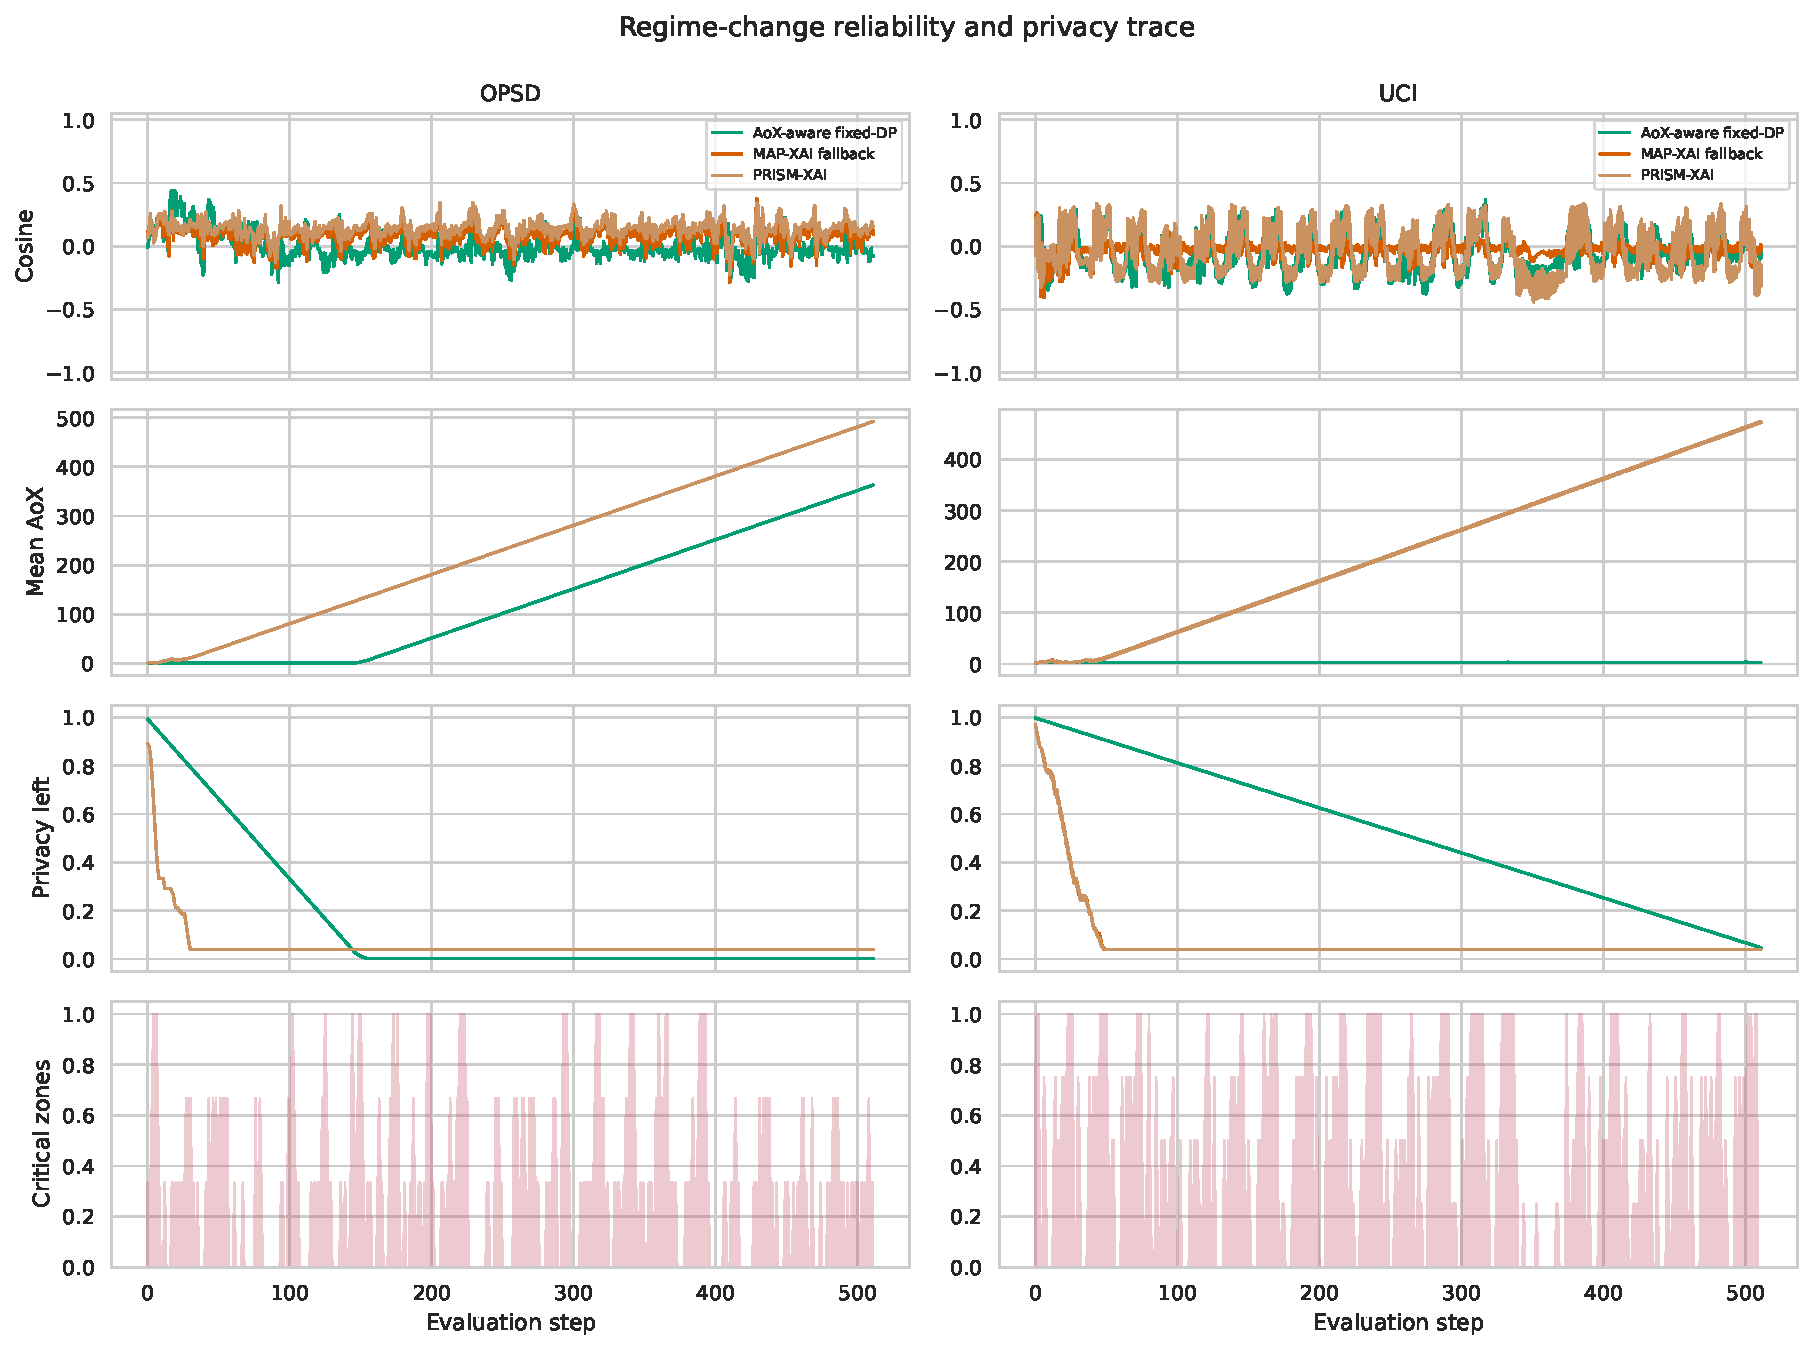
\includegraphics[width=.96\textwidth,height=.82\textheight,keepaspectratio]{../../SERVICE_TRADEOFF_RESULTS/runs/thr_2_cap_8/regime_trace.pdf}

\caption{Public-score threshold $\tau=2$, release cap $M=8$, Combined datasets: representative regime trace. This panel should be read with the setting-level quantitative interpretation and the complete tables immediately preceding the figure block.}

\end{figure*}

\clearpage

\begin{figure*}[p]

\centering

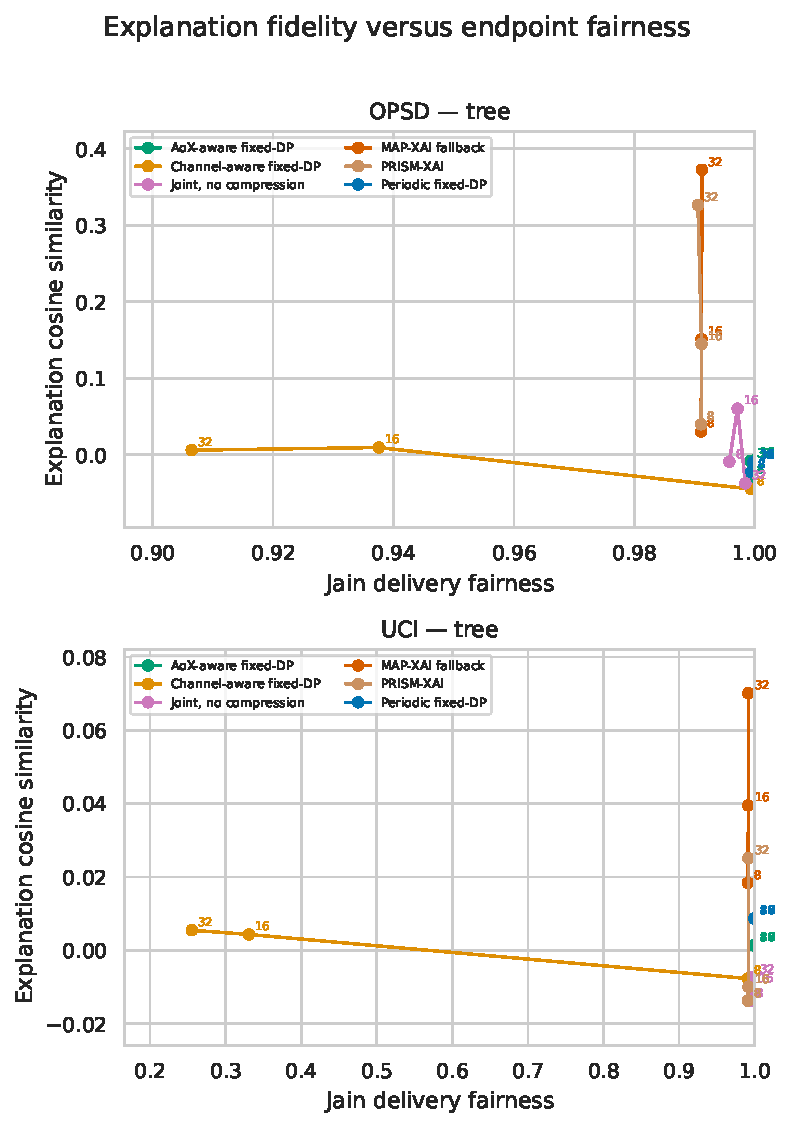
\includegraphics[width=.96\textwidth,height=.82\textheight,keepaspectratio]{../../SERVICE_TRADEOFF_RESULTS/runs/thr_2_cap_8/fairness_reliability.pdf}

\caption{Public-score threshold $\tau=2$, release cap $M=8$, Combined datasets: fairness--reliability plane. This panel should be read with the setting-level quantitative interpretation and the complete tables immediately preceding the figure block.}

\end{figure*}

\clearpage

\begin{figure*}[p]

\centering

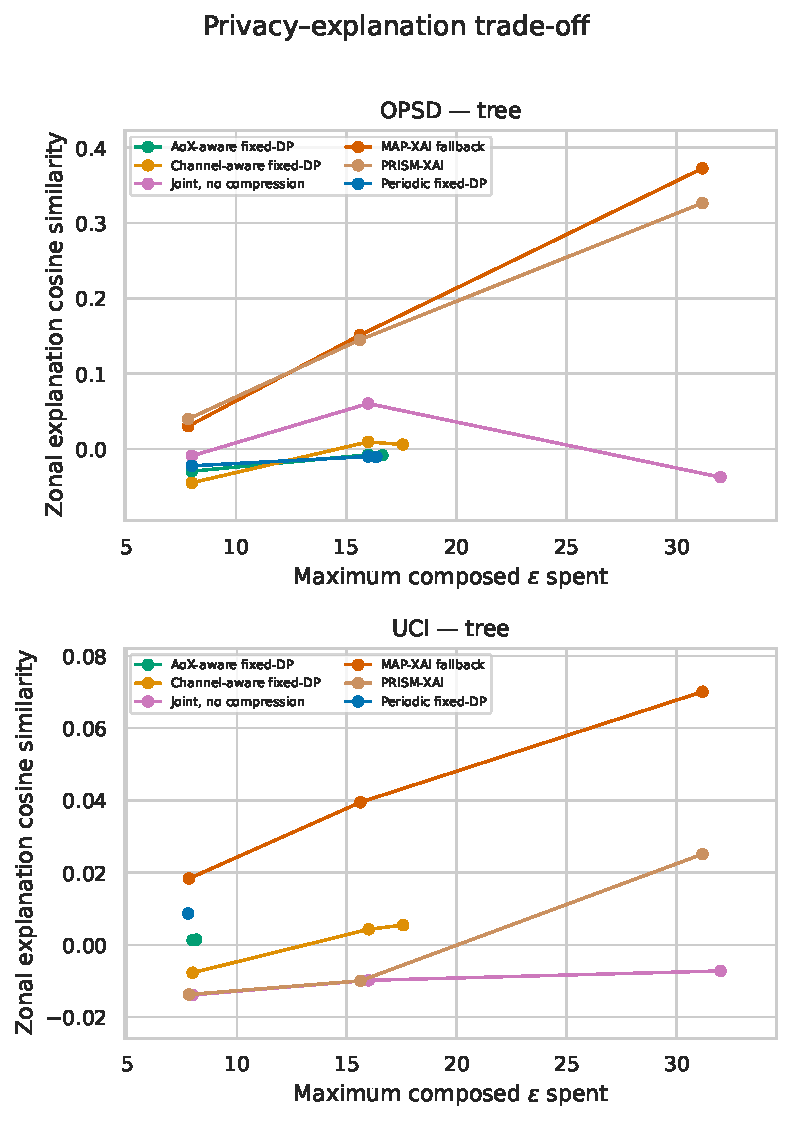
\includegraphics[width=.96\textwidth,height=.82\textheight,keepaspectratio]{../../SERVICE_TRADEOFF_RESULTS/runs/thr_2_cap_8/privacy_fidelity.pdf}

\caption{Public-score threshold $\tau=2$, release cap $M=8$, Combined datasets: privacy--fidelity plane. This panel should be read with the setting-level quantitative interpretation and the complete tables immediately preceding the figure block.}

\end{figure*}

\clearpage

\begin{figure*}[p]

\centering

\includegraphics[width=.96\textwidth,height=.82\textheight,keepaspectratio]{../../SERVICE_TRADEOFF_RESULTS/runs/thr_2_cap_8/pareto_bits_fidelity.pdf}

\caption{Public-score threshold $\tau=2$, release cap $M=8$, Combined datasets: traffic--fidelity Pareto plane. This panel should be read with the setting-level quantitative interpretation and the complete tables immediately preceding the figure block.}

\end{figure*}

\clearpage

\begin{figure*}[p]

\centering

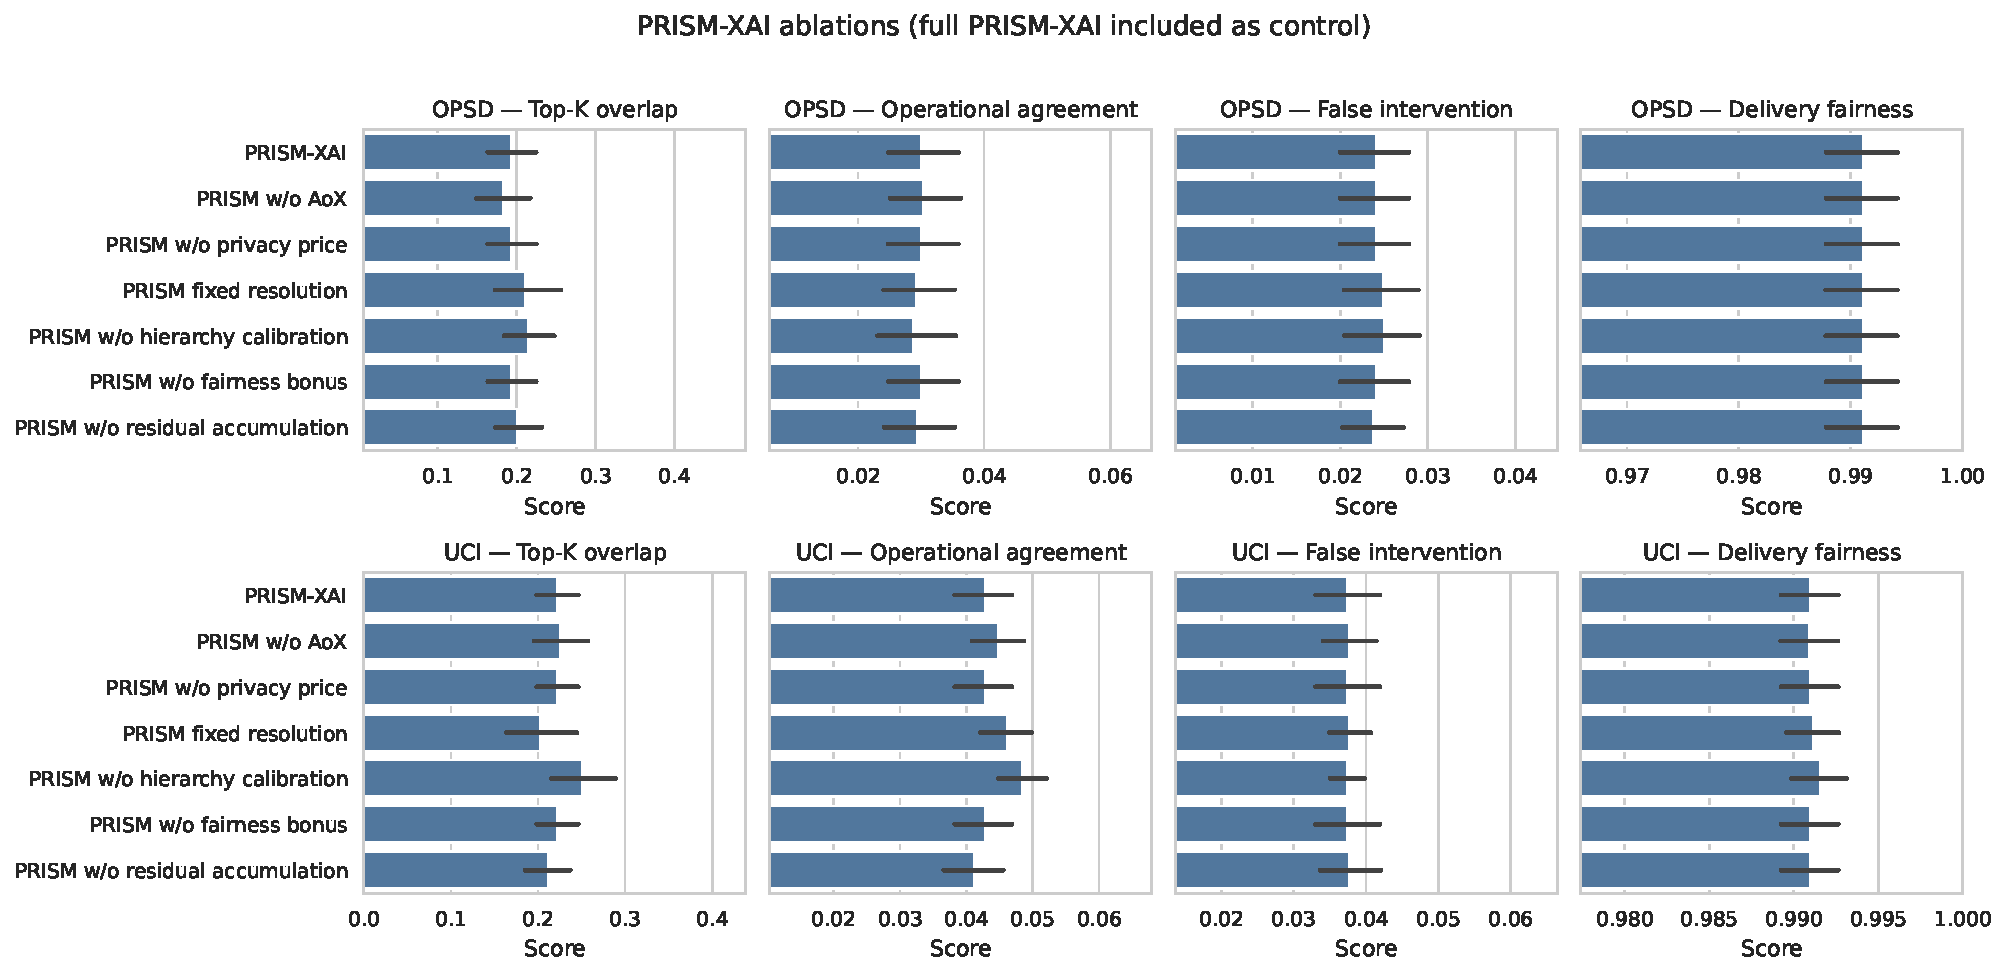
\includegraphics[width=.96\textwidth,height=.82\textheight,keepaspectratio]{../../SERVICE_TRADEOFF_RESULTS/runs/thr_2_cap_8/ablation_results.pdf}

\caption{Public-score threshold $\tau=2$, release cap $M=8$, Combined datasets: component ablation. This panel should be read with the setting-level quantitative interpretation and the complete tables immediately preceding the figure block.}

\end{figure*}

\clearpage

\paragraph{OPSD.} The three generated tables below report the full method means, all condition-level values, and paired differences. The five figures that follow provide the corresponding temporal, fairness, privacy, Pareto, and ablation views. Aggregate panels support the setting-level summary above; dataset panels reveal whether that summary is shared by OPSD and UCI rather than being driven by their different endpoint counts.

\begin{table*}[p]\centering\tiny

\caption{Public-score threshold $\tau=2$, release cap $M=8$, OPSD: complete generated method table.}

\label{tab:thr_2_cap_8:opsd:main}

\resizebox{\linewidth}{!}{% Values are means with 95% Student-t confidence intervals across seeds.
\begin{tabular}{lccccccccccccccc}
\toprule
Dataset & Model & $\epsilon_{\max}$ & Method & Top-$K$ & Cosine & Decision & Recall & Prec. & Abst. & P95 ms & kbit & Spent $\epsilon$ & False int. & bit/correct & Fairness \\
\midrule
OPSD & Tree & 8 & AoX-aware fixed-DP & 0.234 $\pm$ 0.048 & -0.033 $\pm$ 0.028 & 0.119 $\pm$ 0.028 & 0.119 $\pm$ 0.028 & 0.198 $\pm$ 0.054 & 0.721 $\pm$ 0.005 & 6.903 $\pm$ 1.126 & 1560.564 $\pm$ 0.000 & 7.990 $\pm$ 0.000 & 0.183 $\pm$ 0.020 & 35567.482 $\pm$ 10569.818 & 0.999 $\pm$ 0.000 \\
OPSD & Tree & 8 & AoX-aware fixed-DP & 0.238 $\pm$ 0.049 & -0.026 $\pm$ 0.055 & 0.121 $\pm$ 0.026 & 0.121 $\pm$ 0.026 & 0.205 $\pm$ 0.053 & 0.721 $\pm$ 0.005 & 6.903 $\pm$ 1.126 & 1560.564 $\pm$ 0.000 & 7.990 $\pm$ 0.000 & 0.179 $\pm$ 0.023 & 34123.214 $\pm$ 8376.542 & 0.999 $\pm$ 0.000 \\
OPSD & Tree & 8 & Channel-aware fixed-DP & 0.292 $\pm$ 0.037 & -0.041 $\pm$ 0.051 & 0.107 $\pm$ 0.026 & 0.107 $\pm$ 0.026 & 0.217 $\pm$ 0.068 & 0.779 $\pm$ 0.011 & 5.571 $\pm$ 1.784 & 1560.564 $\pm$ 0.000 & 7.990 $\pm$ 0.000 & 0.154 $\pm$ 0.029 & 40860.756 $\pm$ 14126.920 & 0.999 $\pm$ 0.000 \\
OPSD & Tree & 8 & Channel-aware fixed-DP & 0.292 $\pm$ 0.054 & -0.049 $\pm$ 0.064 & 0.111 $\pm$ 0.023 & 0.111 $\pm$ 0.023 & 0.228 $\pm$ 0.066 & 0.779 $\pm$ 0.011 & 5.571 $\pm$ 1.784 & 1560.564 $\pm$ 0.000 & 7.990 $\pm$ 0.000 & 0.149 $\pm$ 0.026 & 37980.855 $\pm$ 12338.094 & 0.999 $\pm$ 0.000 \\
OPSD & Tree & 8 & Joint, no compression & 0.288 $\pm$ 0.064 & -0.030 $\pm$ 0.079 & 0.016 $\pm$ 0.005 & 0.016 $\pm$ 0.005 & 0.193 $\pm$ 0.059 & 0.957 $\pm$ 0.003 & 4.560 $\pm$ 1.811 & 189.900 $\pm$ 0.554 & 7.990 $\pm$ 0.000 & 0.027 $\pm$ 0.005 & 32490.357 $\pm$ 10149.755 & 0.996 $\pm$ 0.002 \\
OPSD & Tree & 8 & Joint, no compression & 0.258 $\pm$ 0.055 & 0.011 $\pm$ 0.094 & 0.019 $\pm$ 0.004 & 0.019 $\pm$ 0.004 & 0.224 $\pm$ 0.044 & 0.957 $\pm$ 0.003 & 4.562 $\pm$ 1.809 & 189.750 $\pm$ 0.566 & 7.990 $\pm$ 0.000 & 0.025 $\pm$ 0.003 & 26079.167 $\pm$ 6335.386 & 0.996 $\pm$ 0.002 \\
OPSD & Tree & 8 & Periodic fixed-DP & 0.241 $\pm$ 0.049 & -0.019 $\pm$ 0.061 & 0.125 $\pm$ 0.020 & 0.125 $\pm$ 0.020 & 0.209 $\pm$ 0.044 & 0.722 $\pm$ 0.006 & 6.303 $\pm$ 1.438 & 1560.564 $\pm$ 0.000 & 7.990 $\pm$ 0.000 & 0.181 $\pm$ 0.021 & 31183.082 $\pm$ 4356.378 & 0.999 $\pm$ 0.000 \\
OPSD & Tree & 8 & Periodic fixed-DP & 0.242 $\pm$ 0.048 & -0.026 $\pm$ 0.082 & 0.135 $\pm$ 0.016 & 0.135 $\pm$ 0.016 & 0.231 $\pm$ 0.037 & 0.722 $\pm$ 0.006 & 6.303 $\pm$ 1.438 & 1560.564 $\pm$ 0.000 & 7.990 $\pm$ 0.000 & 0.169 $\pm$ 0.017 & 28520.235 $\pm$ 3511.595 & 0.999 $\pm$ 0.000 \\
OPSD & Tree & 8 & PRISM-XAI & 0.181 $\pm$ 0.038 & 0.036 $\pm$ 0.059 & 0.031 $\pm$ 0.010 & 0.031 $\pm$ 0.010 & 0.347 $\pm$ 0.128 & 0.938 $\pm$ 0.004 & 4.881 $\pm$ 1.730 & 87.922 $\pm$ 0.587 & 7.823 $\pm$ 0.000 & 0.023 $\pm$ 0.007 & 8276.543 $\pm$ 2832.262 & 0.991 $\pm$ 0.006 \\
OPSD & Tree & 8 & PRISM-XAI & 0.204 $\pm$ 0.062 & 0.043 $\pm$ 0.077 & 0.029 $\pm$ 0.009 & 0.029 $\pm$ 0.009 & 0.330 $\pm$ 0.128 & 0.938 $\pm$ 0.004 & 4.876 $\pm$ 1.737 & 87.707 $\pm$ 0.512 & 7.823 $\pm$ 0.000 & 0.025 $\pm$ 0.007 & 8335.040 $\pm$ 2320.748 & 0.991 $\pm$ 0.006 \\
OPSD & Tree & 8 & MAP-XAI fallback & 0.221 $\pm$ 0.065 & 0.030 $\pm$ 0.075 & 0.029 $\pm$ 0.009 & 0.029 $\pm$ 0.009 & 0.319 $\pm$ 0.121 & 0.938 $\pm$ 0.004 & 4.960 $\pm$ 1.678 & 105.889 $\pm$ 0.169 & 7.823 $\pm$ 0.000 & 0.024 $\pm$ 0.006 & 10646.987 $\pm$ 3613.342 & 0.991 $\pm$ 0.006 \\
OPSD & Tree & 8 & MAP-XAI fallback & 0.192 $\pm$ 0.066 & 0.031 $\pm$ 0.076 & 0.027 $\pm$ 0.007 & 0.027 $\pm$ 0.007 & 0.297 $\pm$ 0.095 & 0.938 $\pm$ 0.004 & 4.960 $\pm$ 1.678 & 105.737 $\pm$ 0.152 & 7.823 $\pm$ 0.000 & 0.026 $\pm$ 0.006 & 10712.923 $\pm$ 2768.192 & 0.991 $\pm$ 0.006 \\
\bottomrule
\end{tabular}
}

\end{table*}\clearpage

\begin{table*}[p]\centering\tiny

\caption{Public-score threshold $\tau=2$, release cap $M=8$, OPSD: complete condition-level generated table.}

\label{tab:thr_2_cap_8:opsd:conditions}

\resizebox{\textwidth}{!}{\begin{tabular}{llllccccccccccc}
\toprule
Dataset & Model & $\epsilon_{\max}$ & Method & kbit & Top-$K$ & Random Top-$K$ & Cosine & Decision & Recall & Precision & Coverage & Abstain & False int. & Spent $\epsilon$ \\
\midrule
OPSD & Tree & 8 & Joint, no compression & 189.900 $\pm$ 0.554 & 0.288 $\pm$ 0.064 & 0.250 $\pm$ 0.000 & -0.030 $\pm$ 0.079 & 0.016 $\pm$ 0.005 & 0.016 $\pm$ 0.005 & 0.193 $\pm$ 0.059 & 0.043 $\pm$ 0.003 & 0.957 $\pm$ 0.003 & 0.027 $\pm$ 0.005 & 7.990 $\pm$ 0.000 \\
OPSD & Tree & 8 & Joint, no compression & 189.750 $\pm$ 0.566 & 0.258 $\pm$ 0.055 & 0.250 $\pm$ 0.000 & 0.011 $\pm$ 0.094 & 0.019 $\pm$ 0.004 & 0.019 $\pm$ 0.004 & 0.224 $\pm$ 0.044 & 0.043 $\pm$ 0.003 & 0.957 $\pm$ 0.003 & 0.025 $\pm$ 0.003 & 7.990 $\pm$ 0.000 \\
OPSD & Tree & 8 & Periodic fixed-DP & 1560.564 $\pm$ 0.000 & 0.241 $\pm$ 0.049 & 0.250 $\pm$ 0.000 & -0.019 $\pm$ 0.061 & 0.125 $\pm$ 0.020 & 0.125 $\pm$ 0.020 & 0.209 $\pm$ 0.044 & 0.278 $\pm$ 0.006 & 0.722 $\pm$ 0.006 & 0.181 $\pm$ 0.021 & 7.990 $\pm$ 0.000 \\
OPSD & Tree & 8 & Periodic fixed-DP & 1560.564 $\pm$ 0.000 & 0.242 $\pm$ 0.048 & 0.250 $\pm$ 0.000 & -0.026 $\pm$ 0.082 & 0.135 $\pm$ 0.016 & 0.135 $\pm$ 0.016 & 0.231 $\pm$ 0.037 & 0.278 $\pm$ 0.006 & 0.722 $\pm$ 0.006 & 0.169 $\pm$ 0.017 & 7.990 $\pm$ 0.000 \\
OPSD & Tree & 8 & PRISM-XAI & 87.922 $\pm$ 0.587 & 0.181 $\pm$ 0.038 & 0.250 $\pm$ 0.000 & 0.036 $\pm$ 0.059 & 0.031 $\pm$ 0.010 & 0.031 $\pm$ 0.010 & 0.347 $\pm$ 0.128 & 0.062 $\pm$ 0.004 & 0.938 $\pm$ 0.004 & 0.023 $\pm$ 0.007 & 7.823 $\pm$ 0.000 \\
OPSD & Tree & 8 & PRISM-XAI & 87.707 $\pm$ 0.512 & 0.204 $\pm$ 0.062 & 0.250 $\pm$ 0.000 & 0.043 $\pm$ 0.077 & 0.029 $\pm$ 0.009 & 0.029 $\pm$ 0.009 & 0.330 $\pm$ 0.128 & 0.062 $\pm$ 0.004 & 0.938 $\pm$ 0.004 & 0.025 $\pm$ 0.007 & 7.823 $\pm$ 0.000 \\
OPSD & Tree & 16 & Joint, no compression & 459.900 $\pm$ 0.750 & 0.232 $\pm$ 0.065 & 0.250 $\pm$ 0.000 & 0.059 $\pm$ 0.048 & 0.038 $\pm$ 0.009 & 0.038 $\pm$ 0.009 & 0.222 $\pm$ 0.049 & 0.088 $\pm$ 0.004 & 0.912 $\pm$ 0.004 & 0.049 $\pm$ 0.005 & 15.997 $\pm$ 0.000 \\
OPSD & Tree & 16 & Joint, no compression & 460.050 $\pm$ 0.724 & 0.241 $\pm$ 0.055 & 0.250 $\pm$ 0.000 & 0.061 $\pm$ 0.052 & 0.039 $\pm$ 0.008 & 0.039 $\pm$ 0.008 & 0.241 $\pm$ 0.042 & 0.088 $\pm$ 0.004 & 0.912 $\pm$ 0.004 & 0.045 $\pm$ 0.004 & 15.997 $\pm$ 0.000 \\
OPSD & Tree & 16 & Periodic fixed-DP & 5112.594 $\pm$ 0.000 & 0.249 $\pm$ 0.022 & 0.250 $\pm$ 0.000 & -0.009 $\pm$ 0.045 & 0.450 $\pm$ 0.062 & 0.450 $\pm$ 0.062 & 0.237 $\pm$ 0.042 & 0.985 $\pm$ 0.002 & 0.015 $\pm$ 0.002 & 0.551 $\pm$ 0.057 & 15.997 $\pm$ 0.000 \\
OPSD & Tree & 16 & Periodic fixed-DP & 5112.594 $\pm$ 0.000 & 0.243 $\pm$ 0.019 & 0.250 $\pm$ 0.000 & -0.012 $\pm$ 0.050 & 0.463 $\pm$ 0.047 & 0.463 $\pm$ 0.047 & 0.240 $\pm$ 0.028 & 0.985 $\pm$ 0.002 & 0.015 $\pm$ 0.002 & 0.547 $\pm$ 0.036 & 15.997 $\pm$ 0.000 \\
OPSD & Tree & 16 & PRISM-XAI & 87.922 $\pm$ 0.597 & 0.221 $\pm$ 0.066 & 0.250 $\pm$ 0.000 & 0.141 $\pm$ 0.056 & 0.029 $\pm$ 0.010 & 0.029 $\pm$ 0.010 & 0.385 $\pm$ 0.148 & 0.062 $\pm$ 0.004 & 0.938 $\pm$ 0.004 & 0.020 $\pm$ 0.007 & 15.620 $\pm$ 0.000 \\
OPSD & Tree & 16 & PRISM-XAI & 87.585 $\pm$ 0.454 & 0.246 $\pm$ 0.046 & 0.250 $\pm$ 0.000 & 0.149 $\pm$ 0.072 & 0.030 $\pm$ 0.008 & 0.030 $\pm$ 0.008 & 0.354 $\pm$ 0.120 & 0.062 $\pm$ 0.004 & 0.938 $\pm$ 0.004 & 0.022 $\pm$ 0.006 & 15.620 $\pm$ 0.000 \\
OPSD & Tree & 32 & Joint, no compression & 1140.900 $\pm$ 7.953 & 0.235 $\pm$ 0.064 & 0.250 $\pm$ 0.000 & -0.031 $\pm$ 0.089 & 0.074 $\pm$ 0.015 & 0.074 $\pm$ 0.015 & 0.205 $\pm$ 0.039 & 0.157 $\pm$ 0.006 & 0.843 $\pm$ 0.006 & 0.107 $\pm$ 0.009 & 31.999 $\pm$ 0.000 \\
OPSD & Tree & 32 & Joint, no compression & 1140.900 $\pm$ 7.953 & 0.282 $\pm$ 0.054 & 0.250 $\pm$ 0.000 & -0.044 $\pm$ 0.076 & 0.080 $\pm$ 0.011 & 0.080 $\pm$ 0.011 & 0.227 $\pm$ 0.052 & 0.158 $\pm$ 0.006 & 0.842 $\pm$ 0.006 & 0.105 $\pm$ 0.015 & 31.999 $\pm$ 0.000 \\
OPSD & Tree & 32 & Periodic fixed-DP & 5299.836 $\pm$ 0.625 & 0.249 $\pm$ 0.022 & 0.250 $\pm$ 0.000 & -0.009 $\pm$ 0.044 & 0.458 $\pm$ 0.066 & 0.458 $\pm$ 0.066 & 0.237 $\pm$ 0.045 & 1.000 $\pm$ 0.000 & 0.000 $\pm$ 0.000 & 0.562 $\pm$ 0.062 & 16.371 $\pm$ 0.000 \\
OPSD & Tree & 32 & Periodic fixed-DP & 5299.836 $\pm$ 0.625 & 0.244 $\pm$ 0.019 & 0.250 $\pm$ 0.000 & -0.012 $\pm$ 0.050 & 0.471 $\pm$ 0.049 & 0.471 $\pm$ 0.049 & 0.240 $\pm$ 0.029 & 1.000 $\pm$ 0.000 & 0.000 $\pm$ 0.000 & 0.559 $\pm$ 0.039 & 16.371 $\pm$ 0.000 \\
OPSD & Tree & 32 & PRISM-XAI & 87.891 $\pm$ 0.540 & 0.397 $\pm$ 0.067 & 0.250 $\pm$ 0.000 & 0.306 $\pm$ 0.044 & 0.040 $\pm$ 0.008 & 0.040 $\pm$ 0.008 & 0.627 $\pm$ 0.190 & 0.063 $\pm$ 0.004 & 0.937 $\pm$ 0.004 & 0.011 $\pm$ 0.007 & 31.175 $\pm$ 0.000 \\
OPSD & Tree & 32 & PRISM-XAI & 87.431 $\pm$ 0.439 & 0.369 $\pm$ 0.054 & 0.250 $\pm$ 0.000 & 0.347 $\pm$ 0.057 & 0.041 $\pm$ 0.006 & 0.041 $\pm$ 0.006 & 0.574 $\pm$ 0.099 & 0.062 $\pm$ 0.004 & 0.938 $\pm$ 0.004 & 0.012 $\pm$ 0.004 & 31.175 $\pm$ 0.000 \\
\bottomrule
\end{tabular}
}

\end{table*}\clearpage

\begin{table*}[p]\centering\tiny

\caption{Public-score threshold $\tau=2$, release cap $M=8$, OPSD: complete generated paired comparisons.}

\label{tab:thr_2_cap_8:opsd:paired}

\resizebox{\textwidth}{!}{\begin{tabular}{llcccc}
\toprule
Dataset & Baseline & Delta kbit & Delta Top-$K$ & Delta recall & Delta fairness \\
\midrule
OPSD & AoX-aware fixed-DP & -1472.642 $\pm$ 0.587 & -0.052 $\pm$ 0.056 & -0.089 $\pm$ 0.033 & -0.008 $\pm$ 0.006 \\
OPSD & AoX-aware fixed-DP & -5011.991 $\pm$ 5.546 & -0.033 $\pm$ 0.086 & -0.372 $\pm$ 0.079 & -0.009 $\pm$ 0.006 \\
OPSD & AoX-aware fixed-DP & -5212.333 $\pm$ 0.540 & 0.144 $\pm$ 0.080 & -0.373 $\pm$ 0.080 & -0.009 $\pm$ 0.006 \\
OPSD & AoX-aware fixed-DP & -1472.857 $\pm$ 0.512 & -0.034 $\pm$ 0.064 & -0.091 $\pm$ 0.028 & -0.008 $\pm$ 0.006 \\
OPSD & AoX-aware fixed-DP & -5012.328 $\pm$ 5.478 & -0.006 $\pm$ 0.062 & -0.385 $\pm$ 0.059 & -0.009 $\pm$ 0.006 \\
OPSD & AoX-aware fixed-DP & -5212.793 $\pm$ 0.439 & 0.117 $\pm$ 0.064 & -0.384 $\pm$ 0.059 & -0.008 $\pm$ 0.006 \\
OPSD & Channel-aware fixed-DP & -1472.642 $\pm$ 0.587 & -0.111 $\pm$ 0.049 & -0.076 $\pm$ 0.029 & -0.008 $\pm$ 0.006 \\
OPSD & Channel-aware fixed-DP & -4598.687 $\pm$ 12.788 & -0.041 $\pm$ 0.083 & -0.372 $\pm$ 0.091 & 0.054 $\pm$ 0.008 \\
OPSD & Channel-aware fixed-DP & -5212.333 $\pm$ 0.540 & 0.139 $\pm$ 0.074 & -0.394 $\pm$ 0.099 & 0.083 $\pm$ 0.008 \\
OPSD & Channel-aware fixed-DP & -1472.857 $\pm$ 0.512 & -0.088 $\pm$ 0.072 & -0.082 $\pm$ 0.026 & -0.008 $\pm$ 0.006 \\
OPSD & Channel-aware fixed-DP & -4599.025 $\pm$ 12.782 & -0.012 $\pm$ 0.057 & -0.389 $\pm$ 0.089 & 0.054 $\pm$ 0.008 \\
OPSD & Channel-aware fixed-DP & -5212.793 $\pm$ 0.439 & 0.112 $\pm$ 0.064 & -0.415 $\pm$ 0.091 & 0.085 $\pm$ 0.008 \\
OPSD & Joint, no compression & -101.978 $\pm$ 0.649 & -0.106 $\pm$ 0.082 & 0.014 $\pm$ 0.009 & -0.005 $\pm$ 0.005 \\
OPSD & Joint, no compression & -371.978 $\pm$ 1.235 & -0.011 $\pm$ 0.086 & -0.009 $\pm$ 0.014 & -0.006 $\pm$ 0.006 \\
OPSD & Joint, no compression & -1053.008 $\pm$ 7.902 & 0.162 $\pm$ 0.100 & -0.034 $\pm$ 0.017 & -0.009 $\pm$ 0.006 \\
OPSD & Joint, no compression & -102.043 $\pm$ 0.542 & -0.054 $\pm$ 0.092 & 0.010 $\pm$ 0.008 & -0.005 $\pm$ 0.005 \\
OPSD & Joint, no compression & -372.466 $\pm$ 0.983 & 0.006 $\pm$ 0.073 & -0.009 $\pm$ 0.011 & -0.006 $\pm$ 0.006 \\
OPSD & Joint, no compression & -1053.469 $\pm$ 8.014 & 0.087 $\pm$ 0.081 & -0.039 $\pm$ 0.013 & -0.007 $\pm$ 0.006 \\
OPSD & Periodic fixed-DP & -1472.642 $\pm$ 0.587 & -0.059 $\pm$ 0.047 & -0.094 $\pm$ 0.024 & -0.008 $\pm$ 0.006 \\
OPSD & Periodic fixed-DP & -5024.672 $\pm$ 0.597 & -0.028 $\pm$ 0.077 & -0.421 $\pm$ 0.066 & -0.009 $\pm$ 0.006 \\
OPSD & Periodic fixed-DP & -5211.944 $\pm$ 0.546 & 0.148 $\pm$ 0.067 & -0.418 $\pm$ 0.066 & -0.010 $\pm$ 0.006 \\
OPSD & Periodic fixed-DP & -1472.857 $\pm$ 0.512 & -0.038 $\pm$ 0.054 & -0.105 $\pm$ 0.018 & -0.008 $\pm$ 0.006 \\
OPSD & Periodic fixed-DP & -5025.010 $\pm$ 0.454 & 0.003 $\pm$ 0.052 & -0.433 $\pm$ 0.050 & -0.009 $\pm$ 0.006 \\
OPSD & Periodic fixed-DP & -5212.405 $\pm$ 0.471 & 0.125 $\pm$ 0.063 & -0.430 $\pm$ 0.050 & -0.009 $\pm$ 0.006 \\
OPSD & MAP-XAI fallback & -17.966 $\pm$ 0.682 & -0.040 $\pm$ 0.046 & 0.002 $\pm$ 0.004 & 0.000 $\pm$ 0.000 \\
OPSD & MAP-XAI fallback & -17.966 $\pm$ 0.687 & -0.043 $\pm$ 0.089 & 0.000 $\pm$ 0.006 & 0.000 $\pm$ 0.000 \\
OPSD & MAP-XAI fallback & -17.997 $\pm$ 0.643 & -0.000 $\pm$ 0.067 & -0.002 $\pm$ 0.005 & -0.001 $\pm$ 0.003 \\
OPSD & MAP-XAI fallback & -18.030 $\pm$ 0.583 & 0.013 $\pm$ 0.040 & 0.003 $\pm$ 0.006 & 0.000 $\pm$ 0.000 \\
OPSD & MAP-XAI fallback & -18.153 $\pm$ 0.544 & 0.003 $\pm$ 0.052 & 0.002 $\pm$ 0.005 & 0.000 $\pm$ 0.000 \\
OPSD & MAP-XAI fallback & -18.121 $\pm$ 0.487 & 0.009 $\pm$ 0.066 & 0.004 $\pm$ 0.005 & 0.000 $\pm$ 0.000 \\
\bottomrule
\end{tabular}
}

\end{table*}\clearpage

\begin{figure*}[p]

\centering

\includegraphics[width=.96\textwidth,height=.82\textheight,keepaspectratio]{../../SERVICE_TRADEOFF_RESULTS/runs/thr_2_cap_8/opsd/regime_trace.pdf}

\caption{Public-score threshold $\tau=2$, release cap $M=8$, OPSD: representative regime trace. This panel should be read with the setting-level quantitative interpretation and the complete tables immediately preceding the figure block.}

\end{figure*}

\clearpage

\begin{figure*}[p]

\centering

\includegraphics[width=.96\textwidth,height=.82\textheight,keepaspectratio]{../../SERVICE_TRADEOFF_RESULTS/runs/thr_2_cap_8/opsd/fairness_reliability.pdf}

\caption{Public-score threshold $\tau=2$, release cap $M=8$, OPSD: fairness--reliability plane. This panel should be read with the setting-level quantitative interpretation and the complete tables immediately preceding the figure block.}

\end{figure*}

\clearpage

\begin{figure*}[p]

\centering

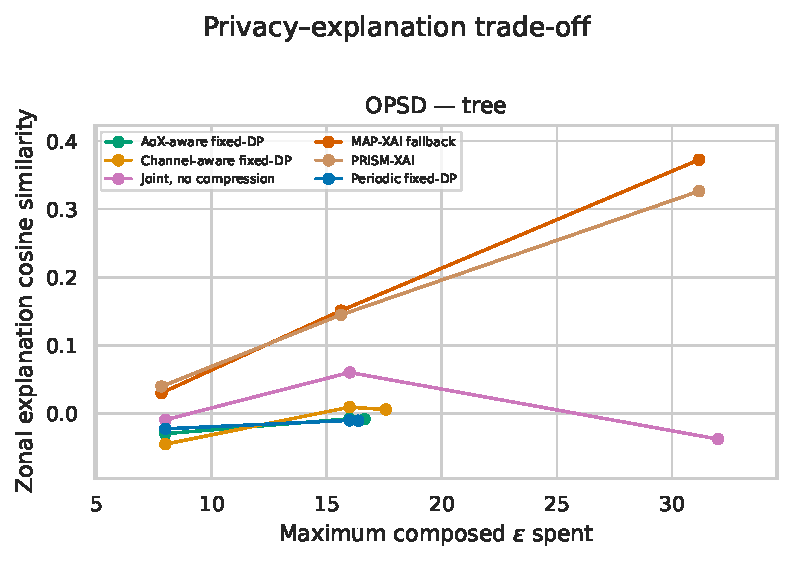
\includegraphics[width=.96\textwidth,height=.82\textheight,keepaspectratio]{../../SERVICE_TRADEOFF_RESULTS/runs/thr_2_cap_8/opsd/privacy_fidelity.pdf}

\caption{Public-score threshold $\tau=2$, release cap $M=8$, OPSD: privacy--fidelity plane. This panel should be read with the setting-level quantitative interpretation and the complete tables immediately preceding the figure block.}

\end{figure*}

\clearpage

\begin{figure*}[p]

\centering

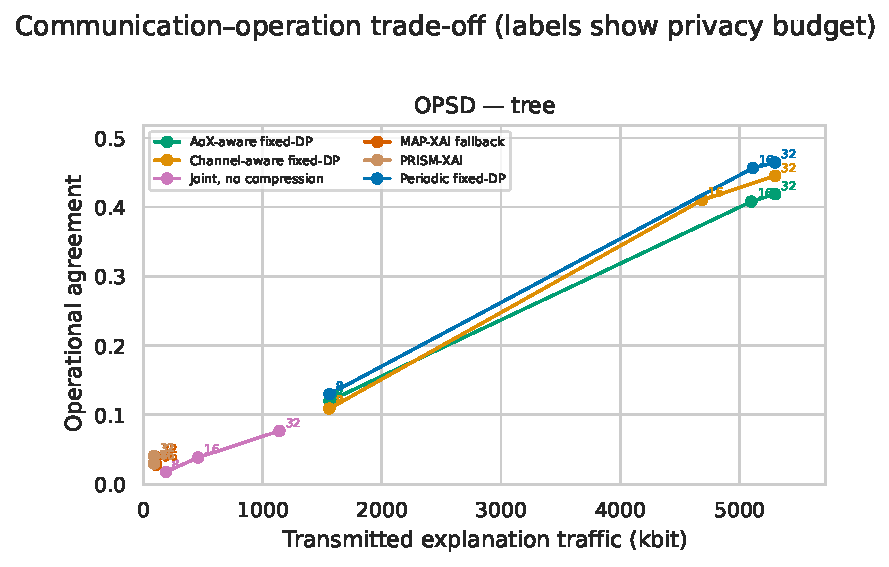
\includegraphics[width=.96\textwidth,height=.82\textheight,keepaspectratio]{../../SERVICE_TRADEOFF_RESULTS/runs/thr_2_cap_8/opsd/pareto_bits_fidelity.pdf}

\caption{Public-score threshold $\tau=2$, release cap $M=8$, OPSD: traffic--fidelity Pareto plane. This panel should be read with the setting-level quantitative interpretation and the complete tables immediately preceding the figure block.}

\end{figure*}

\clearpage

\begin{figure*}[p]

\centering

\includegraphics[width=.96\textwidth,height=.82\textheight,keepaspectratio]{../../SERVICE_TRADEOFF_RESULTS/runs/thr_2_cap_8/opsd/ablation_results.pdf}

\caption{Public-score threshold $\tau=2$, release cap $M=8$, OPSD: component ablation. This panel should be read with the setting-level quantitative interpretation and the complete tables immediately preceding the figure block.}

\end{figure*}

\clearpage

\paragraph{UCI.} The three generated tables below report the full method means, all condition-level values, and paired differences. The five figures that follow provide the corresponding temporal, fairness, privacy, Pareto, and ablation views. Aggregate panels support the setting-level summary above; dataset panels reveal whether that summary is shared by OPSD and UCI rather than being driven by their different endpoint counts.

\begin{table*}[p]\centering\tiny

\caption{Public-score threshold $\tau=2$, release cap $M=8$, UCI: complete generated method table.}

\label{tab:thr_2_cap_8:uci:main}

\resizebox{\linewidth}{!}{% Values are means with 95% Student-t confidence intervals across seeds.
\begin{tabular}{lccccccccccccccc}
\toprule
Dataset & Model & $\epsilon_{\max}$ & Method & Top-$K$ & Cosine & Decision & Recall & Prec. & Abst. & P95 ms & kbit & Spent $\epsilon$ & False int. & bit/correct & Fairness \\
\midrule
UCI & Tree & 8 & AoX-aware fixed-DP & 0.263 $\pm$ 0.041 & -0.007 $\pm$ 0.009 & 0.457 $\pm$ 0.031 & 0.457 $\pm$ 0.031 & 0.362 $\pm$ 0.024 & 0.003 $\pm$ 0.001 & 7.500 $\pm$ 0.000 & 5300.224 $\pm$ 0.000 & 7.990 $\pm$ 0.000 & 0.557 $\pm$ 0.025 & 14002.896 $\pm$ 1040.243 & 0.999 $\pm$ 0.000 \\
UCI & Tree & 8 & AoX-aware fixed-DP & 0.260 $\pm$ 0.022 & 0.010 $\pm$ 0.055 & 0.455 $\pm$ 0.047 & 0.455 $\pm$ 0.047 & 0.361 $\pm$ 0.038 & 0.003 $\pm$ 0.001 & 7.500 $\pm$ 0.000 & 5300.224 $\pm$ 0.000 & 7.990 $\pm$ 0.000 & 0.557 $\pm$ 0.048 & 14198.303 $\pm$ 1508.274 & 0.999 $\pm$ 0.000 \\
UCI & Tree & 8 & Channel-aware fixed-DP & 0.248 $\pm$ 0.031 & 0.004 $\pm$ 0.012 & 0.001 $\pm$ 0.001 & 0.001 $\pm$ 0.001 & 0.150 $\pm$ 0.151 & 0.999 $\pm$ 0.001 & 4.609 $\pm$ 1.781 & 5295.177 $\pm$ 3.740 & 7.990 $\pm$ 0.000 & 0.001 $\pm$ 0.001 & 4632196.500 $\pm$ 2102650.252 & 0.991 $\pm$ 0.001 \\
UCI & Tree & 8 & Channel-aware fixed-DP & 0.239 $\pm$ 0.030 & -0.020 $\pm$ 0.055 & 0.000 $\pm$ 0.000 & 0.000 $\pm$ 0.000 & 0.117 $\pm$ 0.225 & 0.999 $\pm$ 0.001 & 4.609 $\pm$ 1.781 & 5295.177 $\pm$ 3.740 & 7.990 $\pm$ 0.000 & 0.001 $\pm$ 0.001 & 5296989.000 $\pm$ 41104.572 & 0.991 $\pm$ 0.001 \\
UCI & Tree & 8 & Joint, no compression & 0.286 $\pm$ 0.045 & 0.004 $\pm$ 0.020 & 0.052 $\pm$ 0.005 & 0.052 $\pm$ 0.005 & 0.406 $\pm$ 0.037 & 0.875 $\pm$ 0.003 & 5.123 $\pm$ 1.792 & 672.300 $\pm$ 0.452 & 7.990 $\pm$ 0.000 & 0.053 $\pm$ 0.004 & 15676.175 $\pm$ 1475.621 & 0.994 $\pm$ 0.003 \\
UCI & Tree & 8 & Joint, no compression & 0.229 $\pm$ 0.052 & -0.032 $\pm$ 0.050 & 0.057 $\pm$ 0.007 & 0.057 $\pm$ 0.007 & 0.428 $\pm$ 0.041 & 0.875 $\pm$ 0.003 & 5.131 $\pm$ 1.787 & 672.300 $\pm$ 0.452 & 7.990 $\pm$ 0.000 & 0.052 $\pm$ 0.004 & 14702.786 $\pm$ 2334.488 & 0.994 $\pm$ 0.003 \\
UCI & Tree & 8 & Periodic fixed-DP & 0.259 $\pm$ 0.060 & -0.005 $\pm$ 0.008 & 0.006 $\pm$ 0.001 & 0.006 $\pm$ 0.001 & 0.244 $\pm$ 0.049 & 0.989 $\pm$ 0.001 & 4.596 $\pm$ 1.788 & 5299.318 $\pm$ 1.451 & 7.786 $\pm$ 0.000 & 0.013 $\pm$ 0.002 & 1215103.896 $\pm$ 390671.319 & 0.999 $\pm$ 0.000 \\
UCI & Tree & 8 & Periodic fixed-DP & 0.260 $\pm$ 0.044 & 0.022 $\pm$ 0.070 & 0.005 $\pm$ 0.001 & 0.005 $\pm$ 0.001 & 0.195 $\pm$ 0.050 & 0.989 $\pm$ 0.001 & 4.596 $\pm$ 1.788 & 5299.318 $\pm$ 1.451 & 7.786 $\pm$ 0.000 & 0.015 $\pm$ 0.002 & 1555837.203 $\pm$ 955472.503 & 0.999 $\pm$ 0.000 \\
UCI & Tree & 8 & PRISM-XAI & 0.226 $\pm$ 0.039 & -0.007 $\pm$ 0.014 & 0.045 $\pm$ 0.006 & 0.045 $\pm$ 0.006 & 0.448 $\pm$ 0.069 & 0.907 $\pm$ 0.003 & 4.627 $\pm$ 1.490 & 325.204 $\pm$ 1.099 & 7.823 $\pm$ 0.000 & 0.038 $\pm$ 0.006 & 9052.203 $\pm$ 1462.054 & 0.991 $\pm$ 0.002 \\
UCI & Tree & 8 & PRISM-XAI & 0.218 $\pm$ 0.040 & -0.021 $\pm$ 0.077 & 0.041 $\pm$ 0.008 & 0.041 $\pm$ 0.008 & 0.442 $\pm$ 0.091 & 0.912 $\pm$ 0.003 & 4.663 $\pm$ 1.766 & 322.006 $\pm$ 0.783 & 7.823 $\pm$ 0.000 & 0.036 $\pm$ 0.008 & 10546.447 $\pm$ 3413.298 & 0.991 $\pm$ 0.003 \\
UCI & Tree & 8 & MAP-XAI fallback & 0.167 $\pm$ 0.072 & -0.002 $\pm$ 0.015 & 0.047 $\pm$ 0.007 & 0.047 $\pm$ 0.007 & 0.444 $\pm$ 0.055 & 0.907 $\pm$ 0.003 & 4.955 $\pm$ 1.626 & 381.383 $\pm$ 0.421 & 7.823 $\pm$ 0.000 & 0.040 $\pm$ 0.005 & 10267.244 $\pm$ 1941.397 & 0.991 $\pm$ 0.002 \\
UCI & Tree & 8 & MAP-XAI fallback & 0.241 $\pm$ 0.074 & 0.039 $\pm$ 0.065 & 0.046 $\pm$ 0.006 & 0.046 $\pm$ 0.006 & 0.475 $\pm$ 0.053 & 0.909 $\pm$ 0.003 & 5.078 $\pm$ 1.827 & 381.010 $\pm$ 0.445 & 7.823 $\pm$ 0.000 & 0.035 $\pm$ 0.005 & 10274.502 $\pm$ 1367.610 & 0.991 $\pm$ 0.003 \\
\bottomrule
\end{tabular}
}

\end{table*}\clearpage

\begin{table*}[p]\centering\tiny

\caption{Public-score threshold $\tau=2$, release cap $M=8$, UCI: complete condition-level generated table.}

\label{tab:thr_2_cap_8:uci:conditions}

\resizebox{\textwidth}{!}{\begin{tabular}{llllccccccccccc}
\toprule
Dataset & Model & $\epsilon_{\max}$ & Method & kbit & Top-$K$ & Random Top-$K$ & Cosine & Decision & Recall & Precision & Coverage & Abstain & False int. & Spent $\epsilon$ \\
\midrule
UCI & Tree & 8 & Joint, no compression & 672.300 $\pm$ 0.452 & 0.286 $\pm$ 0.045 & 0.250 $\pm$ 0.000 & 0.004 $\pm$ 0.020 & 0.052 $\pm$ 0.005 & 0.052 $\pm$ 0.005 & 0.406 $\pm$ 0.037 & 0.125 $\pm$ 0.003 & 0.875 $\pm$ 0.003 & 0.053 $\pm$ 0.004 & 7.990 $\pm$ 0.000 \\
UCI & Tree & 8 & Joint, no compression & 672.300 $\pm$ 0.452 & 0.229 $\pm$ 0.052 & 0.250 $\pm$ 0.000 & -0.032 $\pm$ 0.050 & 0.057 $\pm$ 0.007 & 0.057 $\pm$ 0.007 & 0.428 $\pm$ 0.041 & 0.125 $\pm$ 0.003 & 0.875 $\pm$ 0.003 & 0.052 $\pm$ 0.004 & 7.990 $\pm$ 0.000 \\
UCI & Tree & 8 & Periodic fixed-DP & 5299.318 $\pm$ 1.451 & 0.259 $\pm$ 0.060 & 0.250 $\pm$ 0.000 & -0.005 $\pm$ 0.008 & 0.006 $\pm$ 0.001 & 0.006 $\pm$ 0.001 & 0.244 $\pm$ 0.049 & 0.011 $\pm$ 0.001 & 0.989 $\pm$ 0.001 & 0.013 $\pm$ 0.002 & 7.786 $\pm$ 0.000 \\
UCI & Tree & 8 & Periodic fixed-DP & 5299.318 $\pm$ 1.451 & 0.260 $\pm$ 0.044 & 0.250 $\pm$ 0.000 & 0.022 $\pm$ 0.070 & 0.005 $\pm$ 0.001 & 0.005 $\pm$ 0.001 & 0.195 $\pm$ 0.050 & 0.011 $\pm$ 0.001 & 0.989 $\pm$ 0.001 & 0.015 $\pm$ 0.002 & 7.786 $\pm$ 0.000 \\
UCI & Tree & 8 & PRISM-XAI & 325.204 $\pm$ 1.099 & 0.226 $\pm$ 0.039 & 0.250 $\pm$ 0.000 & -0.007 $\pm$ 0.014 & 0.045 $\pm$ 0.006 & 0.045 $\pm$ 0.006 & 0.448 $\pm$ 0.069 & 0.093 $\pm$ 0.003 & 0.907 $\pm$ 0.003 & 0.038 $\pm$ 0.006 & 7.823 $\pm$ 0.000 \\
UCI & Tree & 8 & PRISM-XAI & 322.006 $\pm$ 0.783 & 0.218 $\pm$ 0.040 & 0.250 $\pm$ 0.000 & -0.021 $\pm$ 0.077 & 0.041 $\pm$ 0.008 & 0.041 $\pm$ 0.008 & 0.442 $\pm$ 0.091 & 0.088 $\pm$ 0.003 & 0.912 $\pm$ 0.003 & 0.036 $\pm$ 0.008 & 7.823 $\pm$ 0.000 \\
UCI & Tree & 16 & Joint, no compression & 1632.150 $\pm$ 0.339 & 0.216 $\pm$ 0.041 & 0.250 $\pm$ 0.000 & 0.001 $\pm$ 0.012 & 0.094 $\pm$ 0.005 & 0.094 $\pm$ 0.005 & 0.330 $\pm$ 0.024 & 0.228 $\pm$ 0.005 & 0.772 $\pm$ 0.005 & 0.133 $\pm$ 0.010 & 15.997 $\pm$ 0.000 \\
UCI & Tree & 16 & Joint, no compression & 1632.600 $\pm$ 0.554 & 0.204 $\pm$ 0.011 & 0.250 $\pm$ 0.000 & -0.021 $\pm$ 0.033 & 0.099 $\pm$ 0.016 & 0.099 $\pm$ 0.016 & 0.347 $\pm$ 0.054 & 0.228 $\pm$ 0.005 & 0.772 $\pm$ 0.005 & 0.128 $\pm$ 0.011 & 15.997 $\pm$ 0.000 \\
UCI & Tree & 16 & Periodic fixed-DP & 5299.318 $\pm$ 1.451 & 0.259 $\pm$ 0.060 & 0.250 $\pm$ 0.000 & -0.005 $\pm$ 0.008 & 0.006 $\pm$ 0.001 & 0.006 $\pm$ 0.001 & 0.244 $\pm$ 0.049 & 0.011 $\pm$ 0.001 & 0.989 $\pm$ 0.001 & 0.013 $\pm$ 0.002 & 7.786 $\pm$ 0.000 \\
UCI & Tree & 16 & Periodic fixed-DP & 5299.318 $\pm$ 1.451 & 0.260 $\pm$ 0.044 & 0.250 $\pm$ 0.000 & 0.022 $\pm$ 0.070 & 0.005 $\pm$ 0.001 & 0.005 $\pm$ 0.001 & 0.195 $\pm$ 0.050 & 0.011 $\pm$ 0.001 & 0.989 $\pm$ 0.001 & 0.015 $\pm$ 0.002 & 7.786 $\pm$ 0.000 \\
UCI & Tree & 16 & PRISM-XAI & 324.692 $\pm$ 0.734 & 0.260 $\pm$ 0.069 & 0.250 $\pm$ 0.000 & -0.003 $\pm$ 0.016 & 0.041 $\pm$ 0.006 & 0.041 $\pm$ 0.006 & 0.561 $\pm$ 0.104 & 0.090 $\pm$ 0.004 & 0.910 $\pm$ 0.004 & 0.023 $\pm$ 0.006 & 15.620 $\pm$ 0.000 \\
UCI & Tree & 16 & PRISM-XAI & 321.197 $\pm$ 1.037 & 0.247 $\pm$ 0.060 & 0.250 $\pm$ 0.000 & -0.017 $\pm$ 0.061 & 0.038 $\pm$ 0.007 & 0.038 $\pm$ 0.007 & 0.561 $\pm$ 0.070 & 0.081 $\pm$ 0.003 & 0.919 $\pm$ 0.003 & 0.021 $\pm$ 0.004 & 15.620 $\pm$ 0.000 \\
UCI & Tree & 32 & Joint, no compression & 4034.550 $\pm$ 5.034 & 0.246 $\pm$ 0.031 & 0.250 $\pm$ 0.000 & -0.002 $\pm$ 0.015 & 0.228 $\pm$ 0.013 & 0.228 $\pm$ 0.013 & 0.361 $\pm$ 0.028 & 0.537 $\pm$ 0.009 & 0.463 $\pm$ 0.009 & 0.279 $\pm$ 0.017 & 31.999 $\pm$ 0.000 \\
UCI & Tree & 32 & Joint, no compression & 4034.550 $\pm$ 5.034 & 0.241 $\pm$ 0.033 & 0.250 $\pm$ 0.000 & -0.012 $\pm$ 0.030 & 0.228 $\pm$ 0.028 & 0.228 $\pm$ 0.028 & 0.360 $\pm$ 0.047 & 0.530 $\pm$ 0.010 & 0.470 $\pm$ 0.010 & 0.280 $\pm$ 0.026 & 31.999 $\pm$ 0.000 \\
UCI & Tree & 32 & Periodic fixed-DP & 5299.318 $\pm$ 1.451 & 0.259 $\pm$ 0.060 & 0.250 $\pm$ 0.000 & -0.005 $\pm$ 0.008 & 0.006 $\pm$ 0.001 & 0.006 $\pm$ 0.001 & 0.244 $\pm$ 0.049 & 0.011 $\pm$ 0.001 & 0.989 $\pm$ 0.001 & 0.013 $\pm$ 0.002 & 7.786 $\pm$ 0.000 \\
UCI & Tree & 32 & Periodic fixed-DP & 5299.318 $\pm$ 1.451 & 0.260 $\pm$ 0.044 & 0.250 $\pm$ 0.000 & 0.022 $\pm$ 0.070 & 0.005 $\pm$ 0.001 & 0.005 $\pm$ 0.001 & 0.195 $\pm$ 0.050 & 0.011 $\pm$ 0.001 & 0.989 $\pm$ 0.001 & 0.015 $\pm$ 0.002 & 7.786 $\pm$ 0.000 \\
UCI & Tree & 32 & PRISM-XAI & 324.272 $\pm$ 0.853 & 0.285 $\pm$ 0.057 & 0.250 $\pm$ 0.000 & 0.008 $\pm$ 0.016 & 0.039 $\pm$ 0.004 & 0.039 $\pm$ 0.004 & 0.892 $\pm$ 0.052 & 0.081 $\pm$ 0.003 & 0.919 $\pm$ 0.003 & 0.004 $\pm$ 0.002 & 31.175 $\pm$ 0.000 \\
UCI & Tree & 32 & PRISM-XAI & 321.095 $\pm$ 0.887 & 0.246 $\pm$ 0.074 & 0.250 $\pm$ 0.000 & 0.042 $\pm$ 0.069 & 0.036 $\pm$ 0.005 & 0.036 $\pm$ 0.005 & 0.872 $\pm$ 0.111 & 0.076 $\pm$ 0.004 & 0.924 $\pm$ 0.004 & 0.004 $\pm$ 0.004 & 31.175 $\pm$ 0.000 \\
\bottomrule
\end{tabular}
}

\end{table*}\clearpage

\begin{table*}[p]\centering\tiny

\caption{Public-score threshold $\tau=2$, release cap $M=8$, UCI: complete generated paired comparisons.}

\label{tab:thr_2_cap_8:uci:paired}

\resizebox{\textwidth}{!}{\begin{tabular}{llcccc}
\toprule
Dataset & Baseline & Delta kbit & Delta Top-$K$ & Delta recall & Delta fairness \\
\midrule
UCI & AoX-aware fixed-DP & -4975.020 $\pm$ 1.099 & -0.037 $\pm$ 0.046 & -0.412 $\pm$ 0.033 & -0.008 $\pm$ 0.002 \\
UCI & AoX-aware fixed-DP & -4975.532 $\pm$ 0.734 & -0.003 $\pm$ 0.089 & -0.416 $\pm$ 0.028 & -0.007 $\pm$ 0.003 \\
UCI & AoX-aware fixed-DP & -4975.952 $\pm$ 0.853 & 0.021 $\pm$ 0.068 & -0.418 $\pm$ 0.031 & -0.007 $\pm$ 0.002 \\
UCI & AoX-aware fixed-DP & -4978.218 $\pm$ 0.783 & -0.043 $\pm$ 0.038 & -0.414 $\pm$ 0.047 & -0.009 $\pm$ 0.003 \\
UCI & AoX-aware fixed-DP & -4979.027 $\pm$ 1.037 & -0.013 $\pm$ 0.061 & -0.416 $\pm$ 0.044 & -0.007 $\pm$ 0.002 \\
UCI & AoX-aware fixed-DP & -4979.130 $\pm$ 0.887 & -0.014 $\pm$ 0.081 & -0.419 $\pm$ 0.045 & -0.008 $\pm$ 0.002 \\
UCI & Channel-aware fixed-DP & -4969.974 $\pm$ 3.637 & -0.022 $\pm$ 0.056 & 0.044 $\pm$ 0.006 & 0.001 $\pm$ 0.002 \\
UCI & Channel-aware fixed-DP & -4975.532 $\pm$ 0.734 & -0.007 $\pm$ 0.079 & 0.040 $\pm$ 0.006 & 0.661 $\pm$ 0.003 \\
UCI & Channel-aware fixed-DP & -4975.952 $\pm$ 0.853 & 0.016 $\pm$ 0.078 & 0.039 $\pm$ 0.004 & 0.737 $\pm$ 0.002 \\
UCI & Channel-aware fixed-DP & -4973.172 $\pm$ 3.993 & -0.022 $\pm$ 0.051 & 0.041 $\pm$ 0.008 & -0.000 $\pm$ 0.003 \\
UCI & Channel-aware fixed-DP & -4979.027 $\pm$ 1.037 & -0.013 $\pm$ 0.056 & 0.038 $\pm$ 0.007 & 0.661 $\pm$ 0.002 \\
UCI & Channel-aware fixed-DP & -4979.130 $\pm$ 0.887 & -0.013 $\pm$ 0.077 & 0.035 $\pm$ 0.005 & 0.736 $\pm$ 0.002 \\
UCI & Joint, no compression & -347.096 $\pm$ 1.294 & -0.060 $\pm$ 0.070 & -0.007 $\pm$ 0.008 & -0.002 $\pm$ 0.003 \\
UCI & Joint, no compression & -1307.458 $\pm$ 0.943 & 0.044 $\pm$ 0.088 & -0.053 $\pm$ 0.006 & -0.006 $\pm$ 0.002 \\
UCI & Joint, no compression & -3710.278 $\pm$ 4.537 & 0.038 $\pm$ 0.072 & -0.188 $\pm$ 0.014 & -0.007 $\pm$ 0.002 \\
UCI & Joint, no compression & -350.294 $\pm$ 0.927 & -0.012 $\pm$ 0.080 & -0.016 $\pm$ 0.011 & -0.004 $\pm$ 0.004 \\
UCI & Joint, no compression & -1311.403 $\pm$ 0.582 & 0.044 $\pm$ 0.058 & -0.061 $\pm$ 0.019 & -0.006 $\pm$ 0.002 \\
UCI & Joint, no compression & -3713.455 $\pm$ 5.127 & 0.005 $\pm$ 0.053 & -0.192 $\pm$ 0.027 & -0.007 $\pm$ 0.002 \\
UCI & Periodic fixed-DP & -4974.114 $\pm$ 1.995 & -0.033 $\pm$ 0.077 & 0.039 $\pm$ 0.007 & -0.008 $\pm$ 0.002 \\
UCI & Periodic fixed-DP & -4974.626 $\pm$ 1.848 & 0.001 $\pm$ 0.099 & 0.035 $\pm$ 0.007 & -0.008 $\pm$ 0.003 \\
UCI & Periodic fixed-DP & -4975.046 $\pm$ 1.596 & 0.025 $\pm$ 0.092 & 0.033 $\pm$ 0.005 & -0.008 $\pm$ 0.002 \\
UCI & Periodic fixed-DP & -4977.312 $\pm$ 1.437 & -0.043 $\pm$ 0.073 & 0.036 $\pm$ 0.007 & -0.009 $\pm$ 0.003 \\
UCI & Periodic fixed-DP & -4978.121 $\pm$ 1.405 & -0.013 $\pm$ 0.077 & 0.033 $\pm$ 0.007 & -0.007 $\pm$ 0.002 \\
UCI & Periodic fixed-DP & -4978.224 $\pm$ 1.527 & -0.014 $\pm$ 0.101 & 0.030 $\pm$ 0.005 & -0.008 $\pm$ 0.002 \\
UCI & MAP-XAI fallback & -56.179 $\pm$ 0.880 & 0.059 $\pm$ 0.050 & -0.002 $\pm$ 0.004 & 0.000 $\pm$ 0.000 \\
UCI & MAP-XAI fallback & -56.609 $\pm$ 0.650 & 0.023 $\pm$ 0.053 & -0.001 $\pm$ 0.006 & 0.000 $\pm$ 0.001 \\
UCI & MAP-XAI fallback & -56.864 $\pm$ 0.771 & 0.066 $\pm$ 0.045 & -0.003 $\pm$ 0.005 & -0.000 $\pm$ 0.001 \\
UCI & MAP-XAI fallback & -59.004 $\pm$ 0.825 & -0.024 $\pm$ 0.054 & -0.005 $\pm$ 0.004 & -0.000 $\pm$ 0.001 \\
UCI & MAP-XAI fallback & -59.566 $\pm$ 1.156 & 0.043 $\pm$ 0.054 & -0.003 $\pm$ 0.007 & -0.000 $\pm$ 0.001 \\
UCI & MAP-XAI fallback & -59.092 $\pm$ 1.030 & 0.025 $\pm$ 0.105 & -0.002 $\pm$ 0.007 & 0.001 $\pm$ 0.001 \\
\bottomrule
\end{tabular}
}

\end{table*}\clearpage

\begin{figure*}[p]

\centering

\includegraphics[width=.96\textwidth,height=.82\textheight,keepaspectratio]{../../SERVICE_TRADEOFF_RESULTS/runs/thr_2_cap_8/uci/regime_trace.pdf}

\caption{Public-score threshold $\tau=2$, release cap $M=8$, UCI: representative regime trace. This panel should be read with the setting-level quantitative interpretation and the complete tables immediately preceding the figure block.}

\end{figure*}

\clearpage

\begin{figure*}[p]

\centering

\includegraphics[width=.96\textwidth,height=.82\textheight,keepaspectratio]{../../SERVICE_TRADEOFF_RESULTS/runs/thr_2_cap_8/uci/fairness_reliability.pdf}

\caption{Public-score threshold $\tau=2$, release cap $M=8$, UCI: fairness--reliability plane. This panel should be read with the setting-level quantitative interpretation and the complete tables immediately preceding the figure block.}

\end{figure*}

\clearpage

\begin{figure*}[p]

\centering

\includegraphics[width=.96\textwidth,height=.82\textheight,keepaspectratio]{../../SERVICE_TRADEOFF_RESULTS/runs/thr_2_cap_8/uci/privacy_fidelity.pdf}

\caption{Public-score threshold $\tau=2$, release cap $M=8$, UCI: privacy--fidelity plane. This panel should be read with the setting-level quantitative interpretation and the complete tables immediately preceding the figure block.}

\end{figure*}

\clearpage

\begin{figure*}[p]

\centering

\includegraphics[width=.96\textwidth,height=.82\textheight,keepaspectratio]{../../SERVICE_TRADEOFF_RESULTS/runs/thr_2_cap_8/uci/pareto_bits_fidelity.pdf}

\caption{Public-score threshold $\tau=2$, release cap $M=8$, UCI: traffic--fidelity Pareto plane. This panel should be read with the setting-level quantitative interpretation and the complete tables immediately preceding the figure block.}

\end{figure*}

\clearpage

\begin{figure*}[p]

\centering

\includegraphics[width=.96\textwidth,height=.82\textheight,keepaspectratio]{../../SERVICE_TRADEOFF_RESULTS/runs/thr_2_cap_8/uci/ablation_results.pdf}

\caption{Public-score threshold $\tau=2$, release cap $M=8$, UCI: component ablation. This panel should be read with the setting-level quantitative interpretation and the complete tables immediately preceding the figure block.}

\end{figure*}

\clearpage

\subsubsection{Public-score threshold $\tau=3$, release cap $M=8$}

At this operating point, PRISM-XAI transmits 207.31~kbit versus 243.71~kbit for MAP-XAI-only (aggregate-mean ratio saving 14.94\%). The paired difference is -36.40$\pm$3.32~kbit. PRISM coverage is 0.0779, critical-event recall is 0.0366, and maximum recorded expenditure is 18.206. Relative to MAP-XAI-only, the paired coverage change is -0.00010$\pm$0.00043 and recall change is -0.00083$\pm$0.00156. The descriptive overlap rule holds in 12 of 12 cells. Accordingly, this point is read as a matched-service scheduler comparison.

\paragraph{Combined datasets.} The three generated tables below report the full method means, all condition-level values, and paired differences. The five figures that follow provide the corresponding temporal, fairness, privacy, Pareto, and ablation views. Aggregate panels support the setting-level summary above; dataset panels reveal whether that summary is shared by OPSD and UCI rather than being driven by their different endpoint counts.

\begin{table*}[p]\centering\tiny

\caption{Public-score threshold $\tau=3$, release cap $M=8$, Combined datasets: complete generated method table.}

\label{tab:thr_3_cap_8:combined:main}

\resizebox{\linewidth}{!}{% Values are means with 95% Student-t confidence intervals across seeds.
\begin{tabular}{lccccccccccccccc}
\toprule
Dataset & Model & $\epsilon_{\max}$ & Method & Top-$K$ & Cosine & Decision & Recall & Prec. & Abst. & P95 ms & kbit & Spent $\epsilon$ & False int. & bit/correct & Fairness \\
\midrule
OPSD & Tree & 8 & AoX-aware fixed-DP & 0.234 $\pm$ 0.048 & -0.033 $\pm$ 0.028 & 0.119 $\pm$ 0.028 & 0.119 $\pm$ 0.028 & 0.198 $\pm$ 0.054 & 0.721 $\pm$ 0.005 & 6.903 $\pm$ 1.126 & 1560.564 $\pm$ 0.000 & 7.990 $\pm$ 0.000 & 0.183 $\pm$ 0.020 & 35567.482 $\pm$ 10569.818 & 0.999 $\pm$ 0.000 \\
OPSD & Tree & 8 & AoX-aware fixed-DP & 0.238 $\pm$ 0.049 & -0.026 $\pm$ 0.055 & 0.121 $\pm$ 0.026 & 0.121 $\pm$ 0.026 & 0.205 $\pm$ 0.053 & 0.721 $\pm$ 0.005 & 6.903 $\pm$ 1.126 & 1560.564 $\pm$ 0.000 & 7.990 $\pm$ 0.000 & 0.179 $\pm$ 0.023 & 34123.214 $\pm$ 8376.542 & 0.999 $\pm$ 0.000 \\
OPSD & Tree & 8 & Channel-aware fixed-DP & 0.292 $\pm$ 0.037 & -0.041 $\pm$ 0.051 & 0.107 $\pm$ 0.026 & 0.107 $\pm$ 0.026 & 0.217 $\pm$ 0.068 & 0.779 $\pm$ 0.011 & 5.571 $\pm$ 1.784 & 1560.564 $\pm$ 0.000 & 7.990 $\pm$ 0.000 & 0.154 $\pm$ 0.029 & 40860.756 $\pm$ 14126.920 & 0.999 $\pm$ 0.000 \\
OPSD & Tree & 8 & Channel-aware fixed-DP & 0.292 $\pm$ 0.054 & -0.049 $\pm$ 0.064 & 0.111 $\pm$ 0.023 & 0.111 $\pm$ 0.023 & 0.228 $\pm$ 0.066 & 0.779 $\pm$ 0.011 & 5.571 $\pm$ 1.784 & 1560.564 $\pm$ 0.000 & 7.990 $\pm$ 0.000 & 0.149 $\pm$ 0.026 & 37980.855 $\pm$ 12338.094 & 0.999 $\pm$ 0.000 \\
OPSD & Tree & 8 & Joint, no compression & 0.288 $\pm$ 0.064 & -0.030 $\pm$ 0.079 & 0.016 $\pm$ 0.005 & 0.016 $\pm$ 0.005 & 0.193 $\pm$ 0.059 & 0.957 $\pm$ 0.003 & 4.560 $\pm$ 1.811 & 189.900 $\pm$ 0.554 & 7.990 $\pm$ 0.000 & 0.027 $\pm$ 0.005 & 32490.357 $\pm$ 10149.755 & 0.996 $\pm$ 0.002 \\
OPSD & Tree & 8 & Joint, no compression & 0.258 $\pm$ 0.055 & 0.011 $\pm$ 0.094 & 0.019 $\pm$ 0.004 & 0.019 $\pm$ 0.004 & 0.224 $\pm$ 0.044 & 0.957 $\pm$ 0.003 & 4.562 $\pm$ 1.809 & 189.750 $\pm$ 0.566 & 7.990 $\pm$ 0.000 & 0.025 $\pm$ 0.003 & 26079.167 $\pm$ 6335.386 & 0.996 $\pm$ 0.002 \\
OPSD & Tree & 8 & Periodic fixed-DP & 0.241 $\pm$ 0.049 & -0.019 $\pm$ 0.061 & 0.125 $\pm$ 0.020 & 0.125 $\pm$ 0.020 & 0.209 $\pm$ 0.044 & 0.722 $\pm$ 0.006 & 6.303 $\pm$ 1.438 & 1560.564 $\pm$ 0.000 & 7.990 $\pm$ 0.000 & 0.181 $\pm$ 0.021 & 31183.082 $\pm$ 4356.378 & 0.999 $\pm$ 0.000 \\
OPSD & Tree & 8 & Periodic fixed-DP & 0.242 $\pm$ 0.048 & -0.026 $\pm$ 0.082 & 0.135 $\pm$ 0.016 & 0.135 $\pm$ 0.016 & 0.231 $\pm$ 0.037 & 0.722 $\pm$ 0.006 & 6.303 $\pm$ 1.438 & 1560.564 $\pm$ 0.000 & 7.990 $\pm$ 0.000 & 0.169 $\pm$ 0.017 & 28520.235 $\pm$ 3511.595 & 0.999 $\pm$ 0.000 \\
OPSD & Tree & 8 & PRISM-XAI & 0.229 $\pm$ 0.033 & 0.036 $\pm$ 0.077 & 0.027 $\pm$ 0.010 & 0.027 $\pm$ 0.010 & 0.299 $\pm$ 0.119 & 0.929 $\pm$ 0.005 & 4.879 $\pm$ 1.736 & 88.291 $\pm$ 0.526 & 7.823 $\pm$ 0.000 & 0.024 $\pm$ 0.005 & 9900.309 $\pm$ 3435.464 & 0.990 $\pm$ 0.006 \\
OPSD & Tree & 8 & PRISM-XAI & 0.220 $\pm$ 0.042 & 0.038 $\pm$ 0.084 & 0.029 $\pm$ 0.011 & 0.029 $\pm$ 0.011 & 0.301 $\pm$ 0.126 & 0.929 $\pm$ 0.004 & 5.164 $\pm$ 1.832 & 87.953 $\pm$ 0.538 & 7.823 $\pm$ 0.000 & 0.026 $\pm$ 0.006 & 10259.898 $\pm$ 5527.518 & 0.990 $\pm$ 0.006 \\
OPSD & Tree & 8 & MAP-XAI fallback & 0.286 $\pm$ 0.074 & 0.022 $\pm$ 0.080 & 0.028 $\pm$ 0.007 & 0.028 $\pm$ 0.007 & 0.313 $\pm$ 0.084 & 0.929 $\pm$ 0.005 & 4.945 $\pm$ 1.699 & 106.298 $\pm$ 0.291 & 7.823 $\pm$ 0.000 & 0.023 $\pm$ 0.004 & 10008.188 $\pm$ 1905.763 & 0.990 $\pm$ 0.006 \\
OPSD & Tree & 8 & MAP-XAI fallback & 0.232 $\pm$ 0.058 & 0.033 $\pm$ 0.078 & 0.028 $\pm$ 0.007 & 0.028 $\pm$ 0.007 & 0.293 $\pm$ 0.078 & 0.929 $\pm$ 0.004 & 5.230 $\pm$ 1.785 & 106.157 $\pm$ 0.283 & 7.823 $\pm$ 0.000 & 0.026 $\pm$ 0.004 & 9811.388 $\pm$ 1913.898 & 0.990 $\pm$ 0.006 \\
UCI & Tree & 8 & AoX-aware fixed-DP & 0.263 $\pm$ 0.041 & -0.007 $\pm$ 0.009 & 0.457 $\pm$ 0.031 & 0.457 $\pm$ 0.031 & 0.362 $\pm$ 0.024 & 0.003 $\pm$ 0.001 & 7.500 $\pm$ 0.000 & 5300.224 $\pm$ 0.000 & 7.990 $\pm$ 0.000 & 0.557 $\pm$ 0.025 & 14002.896 $\pm$ 1040.243 & 0.999 $\pm$ 0.000 \\
UCI & Tree & 8 & AoX-aware fixed-DP & 0.260 $\pm$ 0.022 & 0.010 $\pm$ 0.055 & 0.455 $\pm$ 0.047 & 0.455 $\pm$ 0.047 & 0.361 $\pm$ 0.038 & 0.003 $\pm$ 0.001 & 7.500 $\pm$ 0.000 & 5300.224 $\pm$ 0.000 & 7.990 $\pm$ 0.000 & 0.557 $\pm$ 0.048 & 14198.303 $\pm$ 1508.274 & 0.999 $\pm$ 0.000 \\
UCI & Tree & 8 & Channel-aware fixed-DP & 0.248 $\pm$ 0.031 & 0.004 $\pm$ 0.012 & 0.001 $\pm$ 0.001 & 0.001 $\pm$ 0.001 & 0.150 $\pm$ 0.151 & 0.999 $\pm$ 0.001 & 4.609 $\pm$ 1.781 & 5295.177 $\pm$ 3.740 & 7.990 $\pm$ 0.000 & 0.001 $\pm$ 0.001 & 4632196.500 $\pm$ 2102650.252 & 0.991 $\pm$ 0.001 \\
UCI & Tree & 8 & Channel-aware fixed-DP & 0.239 $\pm$ 0.030 & -0.020 $\pm$ 0.055 & 0.000 $\pm$ 0.000 & 0.000 $\pm$ 0.000 & 0.117 $\pm$ 0.225 & 0.999 $\pm$ 0.001 & 4.609 $\pm$ 1.781 & 5295.177 $\pm$ 3.740 & 7.990 $\pm$ 0.000 & 0.001 $\pm$ 0.001 & 5296989.000 $\pm$ 41104.572 & 0.991 $\pm$ 0.001 \\
UCI & Tree & 8 & Joint, no compression & 0.286 $\pm$ 0.045 & 0.004 $\pm$ 0.020 & 0.052 $\pm$ 0.005 & 0.052 $\pm$ 0.005 & 0.406 $\pm$ 0.037 & 0.875 $\pm$ 0.003 & 5.123 $\pm$ 1.792 & 672.300 $\pm$ 0.452 & 7.990 $\pm$ 0.000 & 0.053 $\pm$ 0.004 & 15676.175 $\pm$ 1475.621 & 0.994 $\pm$ 0.003 \\
UCI & Tree & 8 & Joint, no compression & 0.229 $\pm$ 0.052 & -0.032 $\pm$ 0.050 & 0.057 $\pm$ 0.007 & 0.057 $\pm$ 0.007 & 0.428 $\pm$ 0.041 & 0.875 $\pm$ 0.003 & 5.131 $\pm$ 1.787 & 672.300 $\pm$ 0.452 & 7.990 $\pm$ 0.000 & 0.052 $\pm$ 0.004 & 14702.786 $\pm$ 2334.488 & 0.994 $\pm$ 0.003 \\
UCI & Tree & 8 & Periodic fixed-DP & 0.259 $\pm$ 0.060 & -0.005 $\pm$ 0.008 & 0.006 $\pm$ 0.001 & 0.006 $\pm$ 0.001 & 0.244 $\pm$ 0.049 & 0.989 $\pm$ 0.001 & 4.596 $\pm$ 1.788 & 5299.318 $\pm$ 1.451 & 7.786 $\pm$ 0.000 & 0.013 $\pm$ 0.002 & 1215103.896 $\pm$ 390671.319 & 0.999 $\pm$ 0.000 \\
UCI & Tree & 8 & Periodic fixed-DP & 0.260 $\pm$ 0.044 & 0.022 $\pm$ 0.070 & 0.005 $\pm$ 0.001 & 0.005 $\pm$ 0.001 & 0.195 $\pm$ 0.050 & 0.989 $\pm$ 0.001 & 4.596 $\pm$ 1.788 & 5299.318 $\pm$ 1.451 & 7.786 $\pm$ 0.000 & 0.015 $\pm$ 0.002 & 1555837.203 $\pm$ 955472.503 & 0.999 $\pm$ 0.000 \\
UCI & Tree & 8 & PRISM-XAI & 0.224 $\pm$ 0.051 & -0.005 $\pm$ 0.014 & 0.040 $\pm$ 0.007 & 0.040 $\pm$ 0.007 & 0.469 $\pm$ 0.065 & 0.910 $\pm$ 0.005 & 5.647 $\pm$ 1.735 & 328.571 $\pm$ 1.335 & 7.823 $\pm$ 0.000 & 0.031 $\pm$ 0.005 & 10347.978 $\pm$ 1665.157 & 0.991 $\pm$ 0.002 \\
UCI & Tree & 8 & PRISM-XAI & 0.228 $\pm$ 0.055 & -0.004 $\pm$ 0.076 & 0.044 $\pm$ 0.009 & 0.044 $\pm$ 0.009 & 0.477 $\pm$ 0.093 & 0.911 $\pm$ 0.005 & 4.164 $\pm$ 1.674 & 325.598 $\pm$ 1.298 & 7.823 $\pm$ 0.000 & 0.033 $\pm$ 0.006 & 9624.204 $\pm$ 2175.413 & 0.992 $\pm$ 0.001 \\
UCI & Tree & 8 & MAP-XAI fallback & 0.178 $\pm$ 0.062 & 0.011 $\pm$ 0.013 & 0.040 $\pm$ 0.005 & 0.040 $\pm$ 0.005 & 0.458 $\pm$ 0.054 & 0.910 $\pm$ 0.005 & 5.670 $\pm$ 1.711 & 381.640 $\pm$ 0.105 & 7.823 $\pm$ 0.000 & 0.033 $\pm$ 0.004 & 11809.010 $\pm$ 1479.313 & 0.991 $\pm$ 0.002 \\
UCI & Tree & 8 & MAP-XAI fallback & 0.211 $\pm$ 0.046 & 0.055 $\pm$ 0.046 & 0.048 $\pm$ 0.009 & 0.048 $\pm$ 0.009 & 0.519 $\pm$ 0.078 & 0.910 $\pm$ 0.005 & 5.202 $\pm$ 1.753 & 381.153 $\pm$ 0.449 & 7.823 $\pm$ 0.000 & 0.031 $\pm$ 0.005 & 10053.490 $\pm$ 2134.182 & 0.992 $\pm$ 0.002 \\
\bottomrule
\end{tabular}
}

\end{table*}\clearpage

\begin{table*}[p]\centering\tiny

\caption{Public-score threshold $\tau=3$, release cap $M=8$, Combined datasets: complete condition-level generated table.}

\label{tab:thr_3_cap_8:combined:conditions}

\resizebox{\textwidth}{!}{\begin{tabular}{llllccccccccccc}
\toprule
Dataset & Model & $\epsilon_{\max}$ & Method & kbit & Top-$K$ & Random Top-$K$ & Cosine & Decision & Recall & Precision & Coverage & Abstain & False int. & Spent $\epsilon$ \\
\midrule
OPSD & Tree & 8 & Joint, no compression & 189.900 $\pm$ 0.554 & 0.288 $\pm$ 0.064 & 0.250 $\pm$ 0.000 & -0.030 $\pm$ 0.079 & 0.016 $\pm$ 0.005 & 0.016 $\pm$ 0.005 & 0.193 $\pm$ 0.059 & 0.043 $\pm$ 0.003 & 0.957 $\pm$ 0.003 & 0.027 $\pm$ 0.005 & 7.990 $\pm$ 0.000 \\
OPSD & Tree & 8 & Joint, no compression & 189.750 $\pm$ 0.566 & 0.258 $\pm$ 0.055 & 0.250 $\pm$ 0.000 & 0.011 $\pm$ 0.094 & 0.019 $\pm$ 0.004 & 0.019 $\pm$ 0.004 & 0.224 $\pm$ 0.044 & 0.043 $\pm$ 0.003 & 0.957 $\pm$ 0.003 & 0.025 $\pm$ 0.003 & 7.990 $\pm$ 0.000 \\
OPSD & Tree & 8 & Periodic fixed-DP & 1560.564 $\pm$ 0.000 & 0.241 $\pm$ 0.049 & 0.250 $\pm$ 0.000 & -0.019 $\pm$ 0.061 & 0.125 $\pm$ 0.020 & 0.125 $\pm$ 0.020 & 0.209 $\pm$ 0.044 & 0.278 $\pm$ 0.006 & 0.722 $\pm$ 0.006 & 0.181 $\pm$ 0.021 & 7.990 $\pm$ 0.000 \\
OPSD & Tree & 8 & Periodic fixed-DP & 1560.564 $\pm$ 0.000 & 0.242 $\pm$ 0.048 & 0.250 $\pm$ 0.000 & -0.026 $\pm$ 0.082 & 0.135 $\pm$ 0.016 & 0.135 $\pm$ 0.016 & 0.231 $\pm$ 0.037 & 0.278 $\pm$ 0.006 & 0.722 $\pm$ 0.006 & 0.169 $\pm$ 0.017 & 7.990 $\pm$ 0.000 \\
OPSD & Tree & 8 & PRISM-XAI & 88.291 $\pm$ 0.526 & 0.229 $\pm$ 0.033 & 0.250 $\pm$ 0.000 & 0.036 $\pm$ 0.077 & 0.027 $\pm$ 0.010 & 0.027 $\pm$ 0.010 & 0.299 $\pm$ 0.119 & 0.071 $\pm$ 0.005 & 0.929 $\pm$ 0.005 & 0.024 $\pm$ 0.005 & 7.823 $\pm$ 0.000 \\
OPSD & Tree & 8 & PRISM-XAI & 87.953 $\pm$ 0.538 & 0.220 $\pm$ 0.042 & 0.250 $\pm$ 0.000 & 0.038 $\pm$ 0.084 & 0.029 $\pm$ 0.011 & 0.029 $\pm$ 0.011 & 0.301 $\pm$ 0.126 & 0.071 $\pm$ 0.004 & 0.929 $\pm$ 0.004 & 0.026 $\pm$ 0.006 & 7.823 $\pm$ 0.000 \\
OPSD & Tree & 16 & Joint, no compression & 459.900 $\pm$ 0.750 & 0.232 $\pm$ 0.065 & 0.250 $\pm$ 0.000 & 0.059 $\pm$ 0.048 & 0.038 $\pm$ 0.009 & 0.038 $\pm$ 0.009 & 0.222 $\pm$ 0.049 & 0.088 $\pm$ 0.004 & 0.912 $\pm$ 0.004 & 0.049 $\pm$ 0.005 & 15.997 $\pm$ 0.000 \\
OPSD & Tree & 16 & Joint, no compression & 460.050 $\pm$ 0.724 & 0.241 $\pm$ 0.055 & 0.250 $\pm$ 0.000 & 0.061 $\pm$ 0.052 & 0.039 $\pm$ 0.008 & 0.039 $\pm$ 0.008 & 0.241 $\pm$ 0.042 & 0.088 $\pm$ 0.004 & 0.912 $\pm$ 0.004 & 0.045 $\pm$ 0.004 & 15.997 $\pm$ 0.000 \\
OPSD & Tree & 16 & Periodic fixed-DP & 5112.594 $\pm$ 0.000 & 0.249 $\pm$ 0.022 & 0.250 $\pm$ 0.000 & -0.009 $\pm$ 0.045 & 0.450 $\pm$ 0.062 & 0.450 $\pm$ 0.062 & 0.237 $\pm$ 0.042 & 0.985 $\pm$ 0.002 & 0.015 $\pm$ 0.002 & 0.551 $\pm$ 0.057 & 15.997 $\pm$ 0.000 \\
OPSD & Tree & 16 & Periodic fixed-DP & 5112.594 $\pm$ 0.000 & 0.243 $\pm$ 0.019 & 0.250 $\pm$ 0.000 & -0.012 $\pm$ 0.050 & 0.463 $\pm$ 0.047 & 0.463 $\pm$ 0.047 & 0.240 $\pm$ 0.028 & 0.985 $\pm$ 0.002 & 0.015 $\pm$ 0.002 & 0.547 $\pm$ 0.036 & 15.997 $\pm$ 0.000 \\
OPSD & Tree & 16 & PRISM-XAI & 88.198 $\pm$ 0.520 & 0.240 $\pm$ 0.048 & 0.250 $\pm$ 0.000 & 0.143 $\pm$ 0.061 & 0.028 $\pm$ 0.008 & 0.028 $\pm$ 0.008 & 0.339 $\pm$ 0.094 & 0.071 $\pm$ 0.004 & 0.929 $\pm$ 0.004 & 0.021 $\pm$ 0.004 & 15.620 $\pm$ 0.000 \\
OPSD & Tree & 16 & PRISM-XAI & 87.769 $\pm$ 0.479 & 0.284 $\pm$ 0.040 & 0.250 $\pm$ 0.000 & 0.171 $\pm$ 0.069 & 0.030 $\pm$ 0.009 & 0.030 $\pm$ 0.009 & 0.339 $\pm$ 0.095 & 0.071 $\pm$ 0.004 & 0.929 $\pm$ 0.004 & 0.022 $\pm$ 0.004 & 15.620 $\pm$ 0.000 \\
OPSD & Tree & 32 & Joint, no compression & 1140.900 $\pm$ 7.953 & 0.235 $\pm$ 0.064 & 0.250 $\pm$ 0.000 & -0.031 $\pm$ 0.089 & 0.074 $\pm$ 0.015 & 0.074 $\pm$ 0.015 & 0.205 $\pm$ 0.039 & 0.157 $\pm$ 0.006 & 0.843 $\pm$ 0.006 & 0.107 $\pm$ 0.009 & 31.999 $\pm$ 0.000 \\
OPSD & Tree & 32 & Joint, no compression & 1140.900 $\pm$ 7.953 & 0.282 $\pm$ 0.054 & 0.250 $\pm$ 0.000 & -0.044 $\pm$ 0.076 & 0.080 $\pm$ 0.011 & 0.080 $\pm$ 0.011 & 0.227 $\pm$ 0.052 & 0.158 $\pm$ 0.006 & 0.842 $\pm$ 0.006 & 0.105 $\pm$ 0.015 & 31.999 $\pm$ 0.000 \\
OPSD & Tree & 32 & Periodic fixed-DP & 5299.836 $\pm$ 0.625 & 0.249 $\pm$ 0.022 & 0.250 $\pm$ 0.000 & -0.009 $\pm$ 0.044 & 0.458 $\pm$ 0.066 & 0.458 $\pm$ 0.066 & 0.237 $\pm$ 0.045 & 1.000 $\pm$ 0.000 & 0.000 $\pm$ 0.000 & 0.562 $\pm$ 0.062 & 16.371 $\pm$ 0.000 \\
OPSD & Tree & 32 & Periodic fixed-DP & 5299.836 $\pm$ 0.625 & 0.244 $\pm$ 0.019 & 0.250 $\pm$ 0.000 & -0.012 $\pm$ 0.050 & 0.471 $\pm$ 0.049 & 0.471 $\pm$ 0.049 & 0.240 $\pm$ 0.029 & 1.000 $\pm$ 0.000 & 0.000 $\pm$ 0.000 & 0.559 $\pm$ 0.039 & 16.371 $\pm$ 0.000 \\
OPSD & Tree & 32 & PRISM-XAI & 88.137 $\pm$ 0.486 & 0.399 $\pm$ 0.059 & 0.250 $\pm$ 0.000 & 0.306 $\pm$ 0.070 & 0.039 $\pm$ 0.009 & 0.039 $\pm$ 0.009 & 0.559 $\pm$ 0.157 & 0.071 $\pm$ 0.004 & 0.929 $\pm$ 0.004 & 0.013 $\pm$ 0.005 & 31.175 $\pm$ 0.000 \\
OPSD & Tree & 32 & PRISM-XAI & 87.554 $\pm$ 0.429 & 0.388 $\pm$ 0.030 & 0.250 $\pm$ 0.000 & 0.359 $\pm$ 0.065 & 0.041 $\pm$ 0.007 & 0.041 $\pm$ 0.007 & 0.531 $\pm$ 0.102 & 0.071 $\pm$ 0.004 & 0.929 $\pm$ 0.004 & 0.014 $\pm$ 0.004 & 31.175 $\pm$ 0.000 \\
UCI & Tree & 8 & Joint, no compression & 672.300 $\pm$ 0.452 & 0.286 $\pm$ 0.045 & 0.250 $\pm$ 0.000 & 0.004 $\pm$ 0.020 & 0.052 $\pm$ 0.005 & 0.052 $\pm$ 0.005 & 0.406 $\pm$ 0.037 & 0.125 $\pm$ 0.003 & 0.875 $\pm$ 0.003 & 0.053 $\pm$ 0.004 & 7.990 $\pm$ 0.000 \\
UCI & Tree & 8 & Joint, no compression & 672.300 $\pm$ 0.452 & 0.229 $\pm$ 0.052 & 0.250 $\pm$ 0.000 & -0.032 $\pm$ 0.050 & 0.057 $\pm$ 0.007 & 0.057 $\pm$ 0.007 & 0.428 $\pm$ 0.041 & 0.125 $\pm$ 0.003 & 0.875 $\pm$ 0.003 & 0.052 $\pm$ 0.004 & 7.990 $\pm$ 0.000 \\
UCI & Tree & 8 & Periodic fixed-DP & 5299.318 $\pm$ 1.451 & 0.259 $\pm$ 0.060 & 0.250 $\pm$ 0.000 & -0.005 $\pm$ 0.008 & 0.006 $\pm$ 0.001 & 0.006 $\pm$ 0.001 & 0.244 $\pm$ 0.049 & 0.011 $\pm$ 0.001 & 0.989 $\pm$ 0.001 & 0.013 $\pm$ 0.002 & 7.786 $\pm$ 0.000 \\
UCI & Tree & 8 & Periodic fixed-DP & 5299.318 $\pm$ 1.451 & 0.260 $\pm$ 0.044 & 0.250 $\pm$ 0.000 & 0.022 $\pm$ 0.070 & 0.005 $\pm$ 0.001 & 0.005 $\pm$ 0.001 & 0.195 $\pm$ 0.050 & 0.011 $\pm$ 0.001 & 0.989 $\pm$ 0.001 & 0.015 $\pm$ 0.002 & 7.786 $\pm$ 0.000 \\
UCI & Tree & 8 & PRISM-XAI & 328.571 $\pm$ 1.335 & 0.224 $\pm$ 0.051 & 0.250 $\pm$ 0.000 & -0.005 $\pm$ 0.014 & 0.040 $\pm$ 0.007 & 0.040 $\pm$ 0.007 & 0.469 $\pm$ 0.065 & 0.090 $\pm$ 0.005 & 0.910 $\pm$ 0.005 & 0.031 $\pm$ 0.005 & 7.823 $\pm$ 0.000 \\
UCI & Tree & 8 & PRISM-XAI & 325.598 $\pm$ 1.298 & 0.228 $\pm$ 0.055 & 0.250 $\pm$ 0.000 & -0.004 $\pm$ 0.076 & 0.044 $\pm$ 0.009 & 0.044 $\pm$ 0.009 & 0.477 $\pm$ 0.093 & 0.089 $\pm$ 0.005 & 0.911 $\pm$ 0.005 & 0.033 $\pm$ 0.006 & 7.823 $\pm$ 0.000 \\
UCI & Tree & 16 & Joint, no compression & 1632.150 $\pm$ 0.339 & 0.216 $\pm$ 0.041 & 0.250 $\pm$ 0.000 & 0.001 $\pm$ 0.012 & 0.094 $\pm$ 0.005 & 0.094 $\pm$ 0.005 & 0.330 $\pm$ 0.024 & 0.228 $\pm$ 0.005 & 0.772 $\pm$ 0.005 & 0.133 $\pm$ 0.010 & 15.997 $\pm$ 0.000 \\
UCI & Tree & 16 & Joint, no compression & 1632.600 $\pm$ 0.554 & 0.204 $\pm$ 0.011 & 0.250 $\pm$ 0.000 & -0.021 $\pm$ 0.033 & 0.099 $\pm$ 0.016 & 0.099 $\pm$ 0.016 & 0.347 $\pm$ 0.054 & 0.228 $\pm$ 0.005 & 0.772 $\pm$ 0.005 & 0.128 $\pm$ 0.011 & 15.997 $\pm$ 0.000 \\
UCI & Tree & 16 & Periodic fixed-DP & 5299.318 $\pm$ 1.451 & 0.259 $\pm$ 0.060 & 0.250 $\pm$ 0.000 & -0.005 $\pm$ 0.008 & 0.006 $\pm$ 0.001 & 0.006 $\pm$ 0.001 & 0.244 $\pm$ 0.049 & 0.011 $\pm$ 0.001 & 0.989 $\pm$ 0.001 & 0.013 $\pm$ 0.002 & 7.786 $\pm$ 0.000 \\
UCI & Tree & 16 & Periodic fixed-DP & 5299.318 $\pm$ 1.451 & 0.260 $\pm$ 0.044 & 0.250 $\pm$ 0.000 & 0.022 $\pm$ 0.070 & 0.005 $\pm$ 0.001 & 0.005 $\pm$ 0.001 & 0.195 $\pm$ 0.050 & 0.011 $\pm$ 0.001 & 0.989 $\pm$ 0.001 & 0.015 $\pm$ 0.002 & 7.786 $\pm$ 0.000 \\
UCI & Tree & 16 & PRISM-XAI & 327.906 $\pm$ 1.114 & 0.246 $\pm$ 0.072 & 0.250 $\pm$ 0.000 & 0.001 $\pm$ 0.014 & 0.043 $\pm$ 0.005 & 0.043 $\pm$ 0.005 & 0.544 $\pm$ 0.057 & 0.090 $\pm$ 0.005 & 0.910 $\pm$ 0.005 & 0.025 $\pm$ 0.004 & 15.620 $\pm$ 0.000 \\
UCI & Tree & 16 & PRISM-XAI & 324.636 $\pm$ 1.010 & 0.225 $\pm$ 0.054 & 0.250 $\pm$ 0.000 & -0.001 $\pm$ 0.073 & 0.043 $\pm$ 0.008 & 0.043 $\pm$ 0.008 & 0.586 $\pm$ 0.085 & 0.084 $\pm$ 0.004 & 0.916 $\pm$ 0.004 & 0.021 $\pm$ 0.005 & 15.620 $\pm$ 0.000 \\
UCI & Tree & 32 & Joint, no compression & 4034.550 $\pm$ 5.034 & 0.246 $\pm$ 0.031 & 0.250 $\pm$ 0.000 & -0.002 $\pm$ 0.015 & 0.228 $\pm$ 0.013 & 0.228 $\pm$ 0.013 & 0.361 $\pm$ 0.028 & 0.537 $\pm$ 0.009 & 0.463 $\pm$ 0.009 & 0.279 $\pm$ 0.017 & 31.999 $\pm$ 0.000 \\
UCI & Tree & 32 & Joint, no compression & 4034.550 $\pm$ 5.034 & 0.241 $\pm$ 0.033 & 0.250 $\pm$ 0.000 & -0.012 $\pm$ 0.030 & 0.228 $\pm$ 0.028 & 0.228 $\pm$ 0.028 & 0.360 $\pm$ 0.047 & 0.530 $\pm$ 0.010 & 0.470 $\pm$ 0.010 & 0.280 $\pm$ 0.026 & 31.999 $\pm$ 0.000 \\
UCI & Tree & 32 & Periodic fixed-DP & 5299.318 $\pm$ 1.451 & 0.259 $\pm$ 0.060 & 0.250 $\pm$ 0.000 & -0.005 $\pm$ 0.008 & 0.006 $\pm$ 0.001 & 0.006 $\pm$ 0.001 & 0.244 $\pm$ 0.049 & 0.011 $\pm$ 0.001 & 0.989 $\pm$ 0.001 & 0.013 $\pm$ 0.002 & 7.786 $\pm$ 0.000 \\
UCI & Tree & 32 & Periodic fixed-DP & 5299.318 $\pm$ 1.451 & 0.260 $\pm$ 0.044 & 0.250 $\pm$ 0.000 & 0.022 $\pm$ 0.070 & 0.005 $\pm$ 0.001 & 0.005 $\pm$ 0.001 & 0.195 $\pm$ 0.050 & 0.011 $\pm$ 0.001 & 0.989 $\pm$ 0.001 & 0.015 $\pm$ 0.002 & 7.786 $\pm$ 0.000 \\
UCI & Tree & 32 & PRISM-XAI & 328.131 $\pm$ 1.290 & 0.274 $\pm$ 0.061 & 0.250 $\pm$ 0.000 & 0.011 $\pm$ 0.017 & 0.038 $\pm$ 0.004 & 0.038 $\pm$ 0.004 & 0.873 $\pm$ 0.070 & 0.083 $\pm$ 0.003 & 0.917 $\pm$ 0.003 & 0.004 $\pm$ 0.003 & 31.175 $\pm$ 0.000 \\
UCI & Tree & 32 & PRISM-XAI & 324.963 $\pm$ 1.575 & 0.273 $\pm$ 0.067 & 0.250 $\pm$ 0.000 & 0.016 $\pm$ 0.096 & 0.037 $\pm$ 0.005 & 0.037 $\pm$ 0.005 & 0.936 $\pm$ 0.069 & 0.073 $\pm$ 0.003 & 0.927 $\pm$ 0.003 & 0.002 $\pm$ 0.003 & 31.175 $\pm$ 0.000 \\
\bottomrule
\end{tabular}
}

\end{table*}\clearpage

\begin{table*}[p]\centering\tiny

\caption{Public-score threshold $\tau=3$, release cap $M=8$, Combined datasets: complete generated paired comparisons.}

\label{tab:thr_3_cap_8:combined:paired}

\resizebox{\textwidth}{!}{\begin{tabular}{llcccc}
\toprule
Dataset & Baseline & Delta kbit & Delta Top-$K$ & Delta recall & Delta fairness \\
\midrule
OPSD & AoX-aware fixed-DP & -1472.273 $\pm$ 0.526 & -0.004 $\pm$ 0.050 & -0.092 $\pm$ 0.035 & -0.009 $\pm$ 0.005 \\
OPSD & AoX-aware fixed-DP & -5011.714 $\pm$ 5.451 & -0.013 $\pm$ 0.080 & -0.373 $\pm$ 0.076 & -0.010 $\pm$ 0.006 \\
OPSD & AoX-aware fixed-DP & -5212.087 $\pm$ 0.486 & 0.146 $\pm$ 0.079 & -0.373 $\pm$ 0.080 & -0.010 $\pm$ 0.006 \\
OPSD & AoX-aware fixed-DP & -1472.611 $\pm$ 0.538 & -0.018 $\pm$ 0.064 & -0.091 $\pm$ 0.034 & -0.009 $\pm$ 0.006 \\
OPSD & AoX-aware fixed-DP & -5012.144 $\pm$ 5.460 & 0.032 $\pm$ 0.058 & -0.384 $\pm$ 0.058 & -0.010 $\pm$ 0.006 \\
OPSD & AoX-aware fixed-DP & -5212.670 $\pm$ 0.429 & 0.136 $\pm$ 0.044 & -0.384 $\pm$ 0.058 & -0.009 $\pm$ 0.006 \\
OPSD & Channel-aware fixed-DP & -1472.273 $\pm$ 0.526 & -0.063 $\pm$ 0.047 & -0.080 $\pm$ 0.032 & -0.009 $\pm$ 0.006 \\
OPSD & Channel-aware fixed-DP & -4598.411 $\pm$ 12.815 & -0.021 $\pm$ 0.068 & -0.373 $\pm$ 0.089 & 0.053 $\pm$ 0.007 \\
OPSD & Channel-aware fixed-DP & -5212.087 $\pm$ 0.486 & 0.141 $\pm$ 0.068 & -0.395 $\pm$ 0.100 & 0.083 $\pm$ 0.007 \\
OPSD & Channel-aware fixed-DP & -1472.611 $\pm$ 0.538 & -0.072 $\pm$ 0.070 & -0.082 $\pm$ 0.030 & -0.009 $\pm$ 0.006 \\
OPSD & Channel-aware fixed-DP & -4598.841 $\pm$ 12.832 & 0.026 $\pm$ 0.054 & -0.389 $\pm$ 0.088 & 0.053 $\pm$ 0.007 \\
OPSD & Channel-aware fixed-DP & -5212.670 $\pm$ 0.429 & 0.131 $\pm$ 0.041 & -0.415 $\pm$ 0.091 & 0.084 $\pm$ 0.008 \\
OPSD & Joint, no compression & -101.609 $\pm$ 0.684 & -0.058 $\pm$ 0.082 & 0.011 $\pm$ 0.010 & -0.005 $\pm$ 0.005 \\
OPSD & Joint, no compression & -371.702 $\pm$ 1.119 & 0.009 $\pm$ 0.094 & -0.010 $\pm$ 0.013 & -0.007 $\pm$ 0.006 \\
OPSD & Joint, no compression & -1052.763 $\pm$ 7.970 & 0.164 $\pm$ 0.086 & -0.035 $\pm$ 0.021 & -0.009 $\pm$ 0.006 \\
OPSD & Joint, no compression & -101.797 $\pm$ 0.692 & -0.038 $\pm$ 0.066 & 0.010 $\pm$ 0.011 & -0.006 $\pm$ 0.005 \\
OPSD & Joint, no compression & -372.281 $\pm$ 1.026 & 0.044 $\pm$ 0.067 & -0.008 $\pm$ 0.013 & -0.007 $\pm$ 0.006 \\
OPSD & Joint, no compression & -1053.346 $\pm$ 8.125 & 0.106 $\pm$ 0.065 & -0.039 $\pm$ 0.016 & -0.008 $\pm$ 0.006 \\
OPSD & Periodic fixed-DP & -1472.273 $\pm$ 0.526 & -0.011 $\pm$ 0.046 & -0.098 $\pm$ 0.026 & -0.009 $\pm$ 0.006 \\
OPSD & Periodic fixed-DP & -5024.396 $\pm$ 0.520 & -0.009 $\pm$ 0.063 & -0.422 $\pm$ 0.063 & -0.009 $\pm$ 0.006 \\
OPSD & Periodic fixed-DP & -5211.699 $\pm$ 0.561 & 0.150 $\pm$ 0.058 & -0.419 $\pm$ 0.067 & -0.010 $\pm$ 0.006 \\
OPSD & Periodic fixed-DP & -1472.611 $\pm$ 0.538 & -0.022 $\pm$ 0.072 & -0.106 $\pm$ 0.022 & -0.009 $\pm$ 0.006 \\
OPSD & Periodic fixed-DP & -5024.825 $\pm$ 0.479 & 0.041 $\pm$ 0.045 & -0.432 $\pm$ 0.050 & -0.010 $\pm$ 0.006 \\
OPSD & Periodic fixed-DP & -5212.282 $\pm$ 0.583 & 0.144 $\pm$ 0.042 & -0.430 $\pm$ 0.050 & -0.010 $\pm$ 0.006 \\
OPSD & MAP-XAI fallback & -18.008 $\pm$ 0.539 & -0.057 $\pm$ 0.060 & -0.001 $\pm$ 0.008 & 0.000 $\pm$ 0.000 \\
OPSD & MAP-XAI fallback & -18.100 $\pm$ 0.509 & -0.057 $\pm$ 0.073 & -0.001 $\pm$ 0.006 & 0.000 $\pm$ 0.000 \\
OPSD & MAP-XAI fallback & -18.058 $\pm$ 0.492 & 0.014 $\pm$ 0.057 & -0.003 $\pm$ 0.007 & -0.001 $\pm$ 0.002 \\
OPSD & MAP-XAI fallback & -18.204 $\pm$ 0.553 & -0.012 $\pm$ 0.070 & 0.001 $\pm$ 0.008 & 0.000 $\pm$ 0.000 \\
OPSD & MAP-XAI fallback & -18.367 $\pm$ 0.475 & 0.029 $\pm$ 0.046 & 0.002 $\pm$ 0.007 & 0.000 $\pm$ 0.000 \\
OPSD & MAP-XAI fallback & -18.273 $\pm$ 0.432 & 0.033 $\pm$ 0.045 & -0.001 $\pm$ 0.006 & 0.000 $\pm$ 0.000 \\
UCI & AoX-aware fixed-DP & -4971.653 $\pm$ 1.335 & -0.039 $\pm$ 0.084 & -0.417 $\pm$ 0.031 & -0.009 $\pm$ 0.002 \\
UCI & AoX-aware fixed-DP & -4972.318 $\pm$ 1.114 & -0.018 $\pm$ 0.091 & -0.415 $\pm$ 0.030 & -0.008 $\pm$ 0.002 \\
UCI & AoX-aware fixed-DP & -4972.093 $\pm$ 1.290 & 0.010 $\pm$ 0.061 & -0.419 $\pm$ 0.032 & -0.008 $\pm$ 0.002 \\
UCI & AoX-aware fixed-DP & -4974.626 $\pm$ 1.298 & -0.032 $\pm$ 0.056 & -0.411 $\pm$ 0.049 & -0.007 $\pm$ 0.001 \\
UCI & AoX-aware fixed-DP & -4975.588 $\pm$ 1.010 & -0.035 $\pm$ 0.047 & -0.411 $\pm$ 0.047 & -0.006 $\pm$ 0.002 \\
UCI & AoX-aware fixed-DP & -4975.261 $\pm$ 1.575 & 0.013 $\pm$ 0.058 & -0.417 $\pm$ 0.047 & -0.006 $\pm$ 0.002 \\
UCI & Channel-aware fixed-DP & -4966.606 $\pm$ 3.827 & -0.024 $\pm$ 0.060 & 0.039 $\pm$ 0.006 & -0.000 $\pm$ 0.002 \\
UCI & Channel-aware fixed-DP & -4972.318 $\pm$ 1.114 & -0.022 $\pm$ 0.079 & 0.042 $\pm$ 0.005 & 0.661 $\pm$ 0.002 \\
UCI & Channel-aware fixed-DP & -4972.093 $\pm$ 1.290 & 0.006 $\pm$ 0.063 & 0.037 $\pm$ 0.005 & 0.736 $\pm$ 0.002 \\
UCI & Channel-aware fixed-DP & -4969.580 $\pm$ 4.222 & -0.011 $\pm$ 0.068 & 0.044 $\pm$ 0.010 & 0.001 $\pm$ 0.001 \\
UCI & Channel-aware fixed-DP & -4975.588 $\pm$ 1.010 & -0.035 $\pm$ 0.050 & 0.043 $\pm$ 0.008 & 0.662 $\pm$ 0.002 \\
UCI & Channel-aware fixed-DP & -4975.261 $\pm$ 1.575 & 0.014 $\pm$ 0.069 & 0.037 $\pm$ 0.005 & 0.738 $\pm$ 0.003 \\
UCI & Joint, no compression & -343.729 $\pm$ 1.578 & -0.061 $\pm$ 0.086 & -0.012 $\pm$ 0.008 & -0.003 $\pm$ 0.003 \\
UCI & Joint, no compression & -1304.244 $\pm$ 1.271 & 0.029 $\pm$ 0.092 & -0.052 $\pm$ 0.006 & -0.006 $\pm$ 0.002 \\
UCI & Joint, no compression & -3706.419 $\pm$ 4.695 & 0.028 $\pm$ 0.058 & -0.190 $\pm$ 0.013 & -0.007 $\pm$ 0.002 \\
UCI & Joint, no compression & -346.702 $\pm$ 1.528 & -0.002 $\pm$ 0.075 & -0.013 $\pm$ 0.012 & -0.002 $\pm$ 0.003 \\
UCI & Joint, no compression & -1307.964 $\pm$ 0.799 & 0.021 $\pm$ 0.051 & -0.056 $\pm$ 0.018 & -0.005 $\pm$ 0.002 \\
UCI & Joint, no compression & -3709.587 $\pm$ 5.063 & 0.032 $\pm$ 0.078 & -0.191 $\pm$ 0.030 & -0.006 $\pm$ 0.002 \\
UCI & Periodic fixed-DP & -4970.747 $\pm$ 1.956 & -0.035 $\pm$ 0.082 & 0.034 $\pm$ 0.007 & -0.009 $\pm$ 0.002 \\
UCI & Periodic fixed-DP & -4971.412 $\pm$ 1.872 & -0.014 $\pm$ 0.077 & 0.037 $\pm$ 0.006 & -0.008 $\pm$ 0.002 \\
UCI & Periodic fixed-DP & -4971.187 $\pm$ 1.698 & 0.015 $\pm$ 0.099 & 0.032 $\pm$ 0.004 & -0.008 $\pm$ 0.002 \\
UCI & Periodic fixed-DP & -4973.721 $\pm$ 1.578 & -0.033 $\pm$ 0.093 & 0.039 $\pm$ 0.008 & -0.007 $\pm$ 0.002 \\
UCI & Periodic fixed-DP & -4974.682 $\pm$ 1.543 & -0.035 $\pm$ 0.074 & 0.038 $\pm$ 0.007 & -0.007 $\pm$ 0.002 \\
UCI & Periodic fixed-DP & -4974.355 $\pm$ 1.546 & 0.013 $\pm$ 0.096 & 0.032 $\pm$ 0.005 & -0.006 $\pm$ 0.002 \\
UCI & MAP-XAI fallback & -53.069 $\pm$ 1.324 & 0.047 $\pm$ 0.064 & 0.000 $\pm$ 0.005 & 0.000 $\pm$ 0.000 \\
UCI & MAP-XAI fallback & -53.673 $\pm$ 1.109 & 0.023 $\pm$ 0.057 & 0.001 $\pm$ 0.004 & -0.000 $\pm$ 0.001 \\
UCI & MAP-XAI fallback & -53.427 $\pm$ 1.194 & 0.041 $\pm$ 0.046 & -0.004 $\pm$ 0.004 & -0.000 $\pm$ 0.001 \\
UCI & MAP-XAI fallback & -55.556 $\pm$ 1.430 & 0.017 $\pm$ 0.054 & -0.004 $\pm$ 0.007 & 0.000 $\pm$ 0.000 \\
UCI & MAP-XAI fallback & -56.375 $\pm$ 1.113 & -0.005 $\pm$ 0.048 & 0.001 $\pm$ 0.007 & 0.001 $\pm$ 0.002 \\
UCI & MAP-XAI fallback & -55.666 $\pm$ 1.169 & -0.026 $\pm$ 0.079 & -0.001 $\pm$ 0.006 & 0.000 $\pm$ 0.001 \\
\bottomrule
\end{tabular}
}

\end{table*}\clearpage

\begin{figure*}[p]

\centering

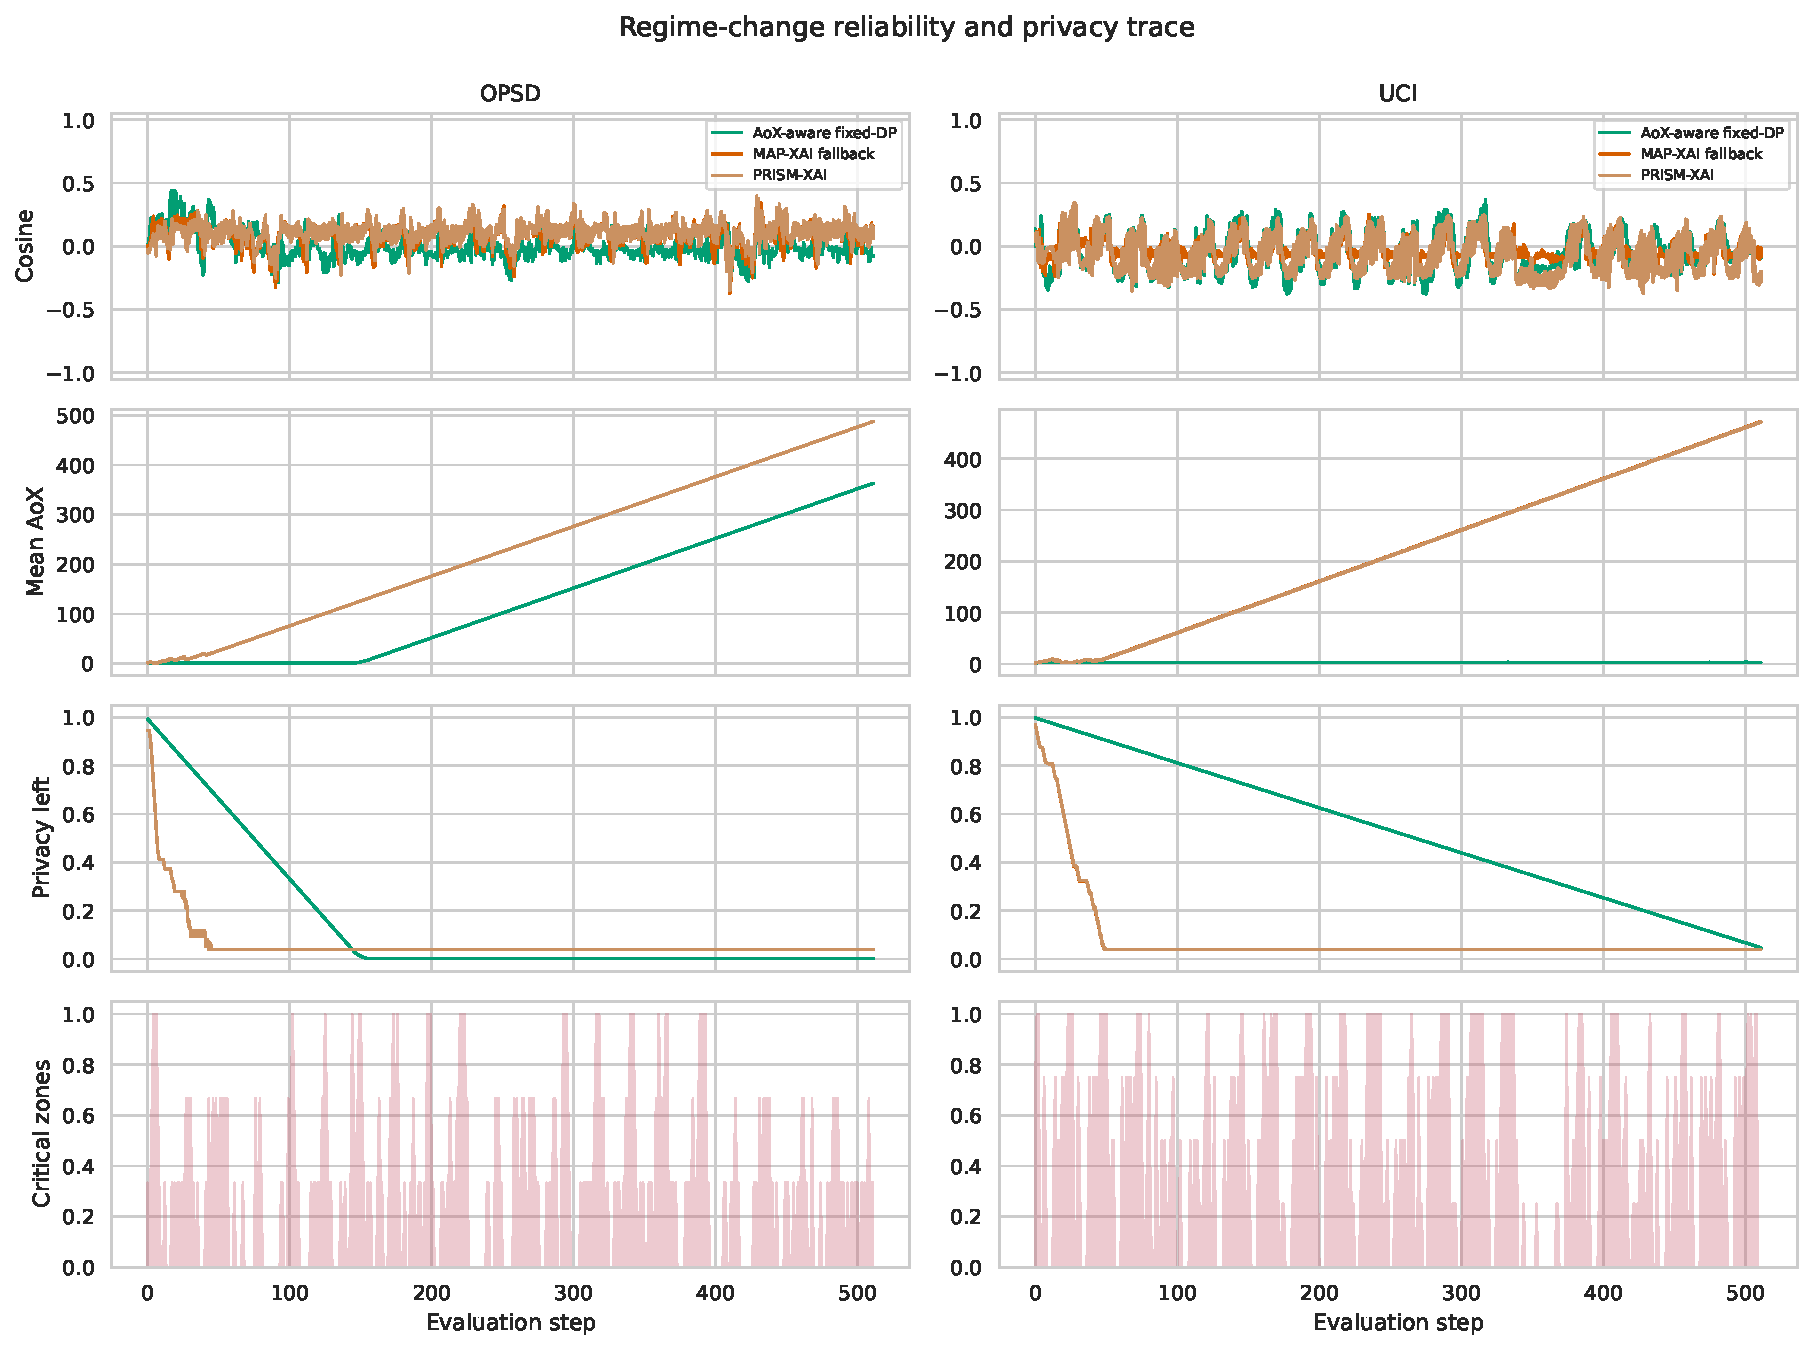
\includegraphics[width=.96\textwidth,height=.82\textheight,keepaspectratio]{../../SERVICE_TRADEOFF_RESULTS/runs/thr_3_cap_8/regime_trace.pdf}

\caption{Public-score threshold $\tau=3$, release cap $M=8$, Combined datasets: representative regime trace. This panel should be read with the setting-level quantitative interpretation and the complete tables immediately preceding the figure block.}

\end{figure*}

\clearpage

\begin{figure*}[p]

\centering

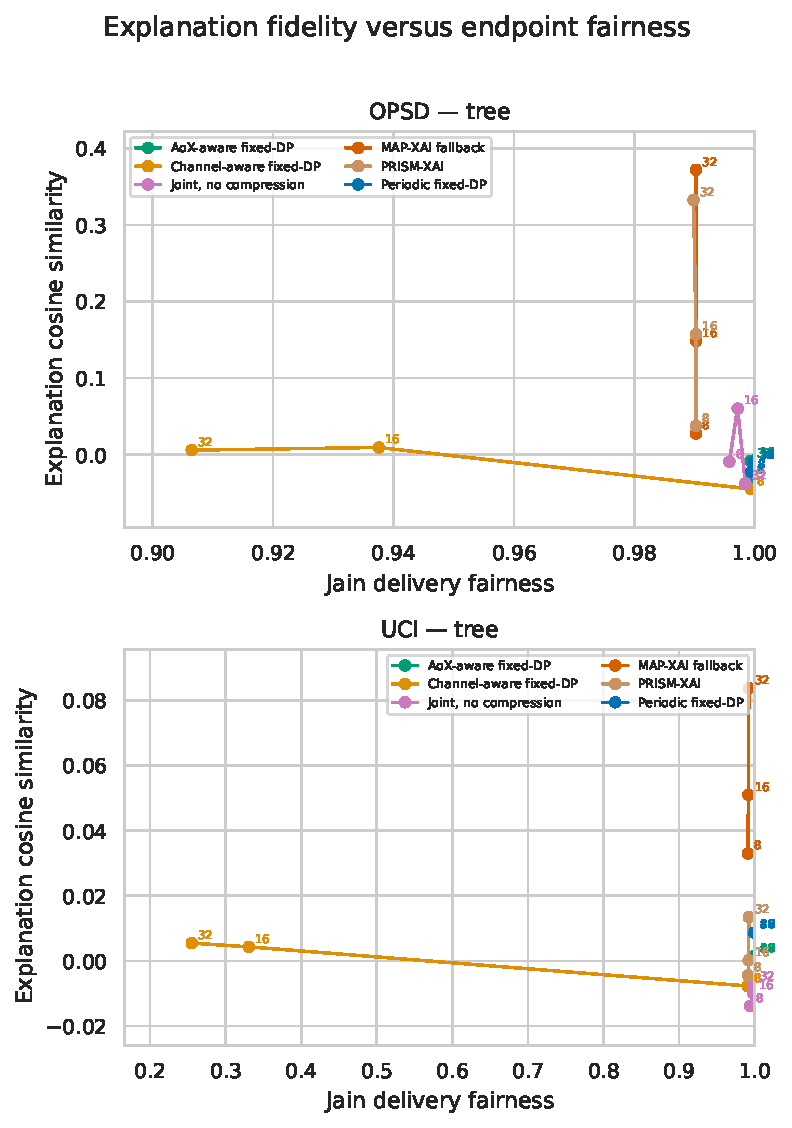
\includegraphics[width=.96\textwidth,height=.82\textheight,keepaspectratio]{../../SERVICE_TRADEOFF_RESULTS/runs/thr_3_cap_8/fairness_reliability.pdf}

\caption{Public-score threshold $\tau=3$, release cap $M=8$, Combined datasets: fairness--reliability plane. This panel should be read with the setting-level quantitative interpretation and the complete tables immediately preceding the figure block.}

\end{figure*}

\clearpage

\begin{figure*}[p]

\centering

\includegraphics[width=.96\textwidth,height=.82\textheight,keepaspectratio]{../../SERVICE_TRADEOFF_RESULTS/runs/thr_3_cap_8/privacy_fidelity.pdf}

\caption{Public-score threshold $\tau=3$, release cap $M=8$, Combined datasets: privacy--fidelity plane. This panel should be read with the setting-level quantitative interpretation and the complete tables immediately preceding the figure block.}

\end{figure*}

\clearpage

\begin{figure*}[p]

\centering

\includegraphics[width=.96\textwidth,height=.82\textheight,keepaspectratio]{../../SERVICE_TRADEOFF_RESULTS/runs/thr_3_cap_8/pareto_bits_fidelity.pdf}

\caption{Public-score threshold $\tau=3$, release cap $M=8$, Combined datasets: traffic--fidelity Pareto plane. This panel should be read with the setting-level quantitative interpretation and the complete tables immediately preceding the figure block.}

\end{figure*}

\clearpage

\begin{figure*}[p]

\centering

\includegraphics[width=.96\textwidth,height=.82\textheight,keepaspectratio]{../../SERVICE_TRADEOFF_RESULTS/runs/thr_3_cap_8/ablation_results.pdf}

\caption{Public-score threshold $\tau=3$, release cap $M=8$, Combined datasets: component ablation. This panel should be read with the setting-level quantitative interpretation and the complete tables immediately preceding the figure block.}

\end{figure*}

\clearpage

\paragraph{OPSD.} The three generated tables below report the full method means, all condition-level values, and paired differences. The five figures that follow provide the corresponding temporal, fairness, privacy, Pareto, and ablation views. Aggregate panels support the setting-level summary above; dataset panels reveal whether that summary is shared by OPSD and UCI rather than being driven by their different endpoint counts.

\begin{table*}[p]\centering\tiny

\caption{Public-score threshold $\tau=3$, release cap $M=8$, OPSD: complete generated method table.}

\label{tab:thr_3_cap_8:opsd:main}

\resizebox{\linewidth}{!}{% Values are means with 95% Student-t confidence intervals across seeds.
\begin{tabular}{lccccccccccccccc}
\toprule
Dataset & Model & $\epsilon_{\max}$ & Method & Top-$K$ & Cosine & Decision & Recall & Prec. & Abst. & P95 ms & kbit & Spent $\epsilon$ & False int. & bit/correct & Fairness \\
\midrule
OPSD & Tree & 8 & AoX-aware fixed-DP & 0.234 $\pm$ 0.048 & -0.033 $\pm$ 0.028 & 0.119 $\pm$ 0.028 & 0.119 $\pm$ 0.028 & 0.198 $\pm$ 0.054 & 0.721 $\pm$ 0.005 & 6.903 $\pm$ 1.126 & 1560.564 $\pm$ 0.000 & 7.990 $\pm$ 0.000 & 0.183 $\pm$ 0.020 & 35567.482 $\pm$ 10569.818 & 0.999 $\pm$ 0.000 \\
OPSD & Tree & 8 & AoX-aware fixed-DP & 0.238 $\pm$ 0.049 & -0.026 $\pm$ 0.055 & 0.121 $\pm$ 0.026 & 0.121 $\pm$ 0.026 & 0.205 $\pm$ 0.053 & 0.721 $\pm$ 0.005 & 6.903 $\pm$ 1.126 & 1560.564 $\pm$ 0.000 & 7.990 $\pm$ 0.000 & 0.179 $\pm$ 0.023 & 34123.214 $\pm$ 8376.542 & 0.999 $\pm$ 0.000 \\
OPSD & Tree & 8 & Channel-aware fixed-DP & 0.292 $\pm$ 0.037 & -0.041 $\pm$ 0.051 & 0.107 $\pm$ 0.026 & 0.107 $\pm$ 0.026 & 0.217 $\pm$ 0.068 & 0.779 $\pm$ 0.011 & 5.571 $\pm$ 1.784 & 1560.564 $\pm$ 0.000 & 7.990 $\pm$ 0.000 & 0.154 $\pm$ 0.029 & 40860.756 $\pm$ 14126.920 & 0.999 $\pm$ 0.000 \\
OPSD & Tree & 8 & Channel-aware fixed-DP & 0.292 $\pm$ 0.054 & -0.049 $\pm$ 0.064 & 0.111 $\pm$ 0.023 & 0.111 $\pm$ 0.023 & 0.228 $\pm$ 0.066 & 0.779 $\pm$ 0.011 & 5.571 $\pm$ 1.784 & 1560.564 $\pm$ 0.000 & 7.990 $\pm$ 0.000 & 0.149 $\pm$ 0.026 & 37980.855 $\pm$ 12338.094 & 0.999 $\pm$ 0.000 \\
OPSD & Tree & 8 & Joint, no compression & 0.288 $\pm$ 0.064 & -0.030 $\pm$ 0.079 & 0.016 $\pm$ 0.005 & 0.016 $\pm$ 0.005 & 0.193 $\pm$ 0.059 & 0.957 $\pm$ 0.003 & 4.560 $\pm$ 1.811 & 189.900 $\pm$ 0.554 & 7.990 $\pm$ 0.000 & 0.027 $\pm$ 0.005 & 32490.357 $\pm$ 10149.755 & 0.996 $\pm$ 0.002 \\
OPSD & Tree & 8 & Joint, no compression & 0.258 $\pm$ 0.055 & 0.011 $\pm$ 0.094 & 0.019 $\pm$ 0.004 & 0.019 $\pm$ 0.004 & 0.224 $\pm$ 0.044 & 0.957 $\pm$ 0.003 & 4.562 $\pm$ 1.809 & 189.750 $\pm$ 0.566 & 7.990 $\pm$ 0.000 & 0.025 $\pm$ 0.003 & 26079.167 $\pm$ 6335.386 & 0.996 $\pm$ 0.002 \\
OPSD & Tree & 8 & Periodic fixed-DP & 0.241 $\pm$ 0.049 & -0.019 $\pm$ 0.061 & 0.125 $\pm$ 0.020 & 0.125 $\pm$ 0.020 & 0.209 $\pm$ 0.044 & 0.722 $\pm$ 0.006 & 6.303 $\pm$ 1.438 & 1560.564 $\pm$ 0.000 & 7.990 $\pm$ 0.000 & 0.181 $\pm$ 0.021 & 31183.082 $\pm$ 4356.378 & 0.999 $\pm$ 0.000 \\
OPSD & Tree & 8 & Periodic fixed-DP & 0.242 $\pm$ 0.048 & -0.026 $\pm$ 0.082 & 0.135 $\pm$ 0.016 & 0.135 $\pm$ 0.016 & 0.231 $\pm$ 0.037 & 0.722 $\pm$ 0.006 & 6.303 $\pm$ 1.438 & 1560.564 $\pm$ 0.000 & 7.990 $\pm$ 0.000 & 0.169 $\pm$ 0.017 & 28520.235 $\pm$ 3511.595 & 0.999 $\pm$ 0.000 \\
OPSD & Tree & 8 & PRISM-XAI & 0.229 $\pm$ 0.033 & 0.036 $\pm$ 0.077 & 0.027 $\pm$ 0.010 & 0.027 $\pm$ 0.010 & 0.299 $\pm$ 0.119 & 0.929 $\pm$ 0.005 & 4.879 $\pm$ 1.736 & 88.291 $\pm$ 0.526 & 7.823 $\pm$ 0.000 & 0.024 $\pm$ 0.005 & 9900.309 $\pm$ 3435.464 & 0.990 $\pm$ 0.006 \\
OPSD & Tree & 8 & PRISM-XAI & 0.220 $\pm$ 0.042 & 0.038 $\pm$ 0.084 & 0.029 $\pm$ 0.011 & 0.029 $\pm$ 0.011 & 0.301 $\pm$ 0.126 & 0.929 $\pm$ 0.004 & 5.164 $\pm$ 1.832 & 87.953 $\pm$ 0.538 & 7.823 $\pm$ 0.000 & 0.026 $\pm$ 0.006 & 10259.898 $\pm$ 5527.518 & 0.990 $\pm$ 0.006 \\
OPSD & Tree & 8 & MAP-XAI fallback & 0.286 $\pm$ 0.074 & 0.022 $\pm$ 0.080 & 0.028 $\pm$ 0.007 & 0.028 $\pm$ 0.007 & 0.313 $\pm$ 0.084 & 0.929 $\pm$ 0.005 & 4.945 $\pm$ 1.699 & 106.298 $\pm$ 0.291 & 7.823 $\pm$ 0.000 & 0.023 $\pm$ 0.004 & 10008.188 $\pm$ 1905.763 & 0.990 $\pm$ 0.006 \\
OPSD & Tree & 8 & MAP-XAI fallback & 0.232 $\pm$ 0.058 & 0.033 $\pm$ 0.078 & 0.028 $\pm$ 0.007 & 0.028 $\pm$ 0.007 & 0.293 $\pm$ 0.078 & 0.929 $\pm$ 0.004 & 5.230 $\pm$ 1.785 & 106.157 $\pm$ 0.283 & 7.823 $\pm$ 0.000 & 0.026 $\pm$ 0.004 & 9811.388 $\pm$ 1913.898 & 0.990 $\pm$ 0.006 \\
\bottomrule
\end{tabular}
}

\end{table*}\clearpage

\begin{table*}[p]\centering\tiny

\caption{Public-score threshold $\tau=3$, release cap $M=8$, OPSD: complete condition-level generated table.}

\label{tab:thr_3_cap_8:opsd:conditions}

\resizebox{\textwidth}{!}{\begin{tabular}{llllccccccccccc}
\toprule
Dataset & Model & $\epsilon_{\max}$ & Method & kbit & Top-$K$ & Random Top-$K$ & Cosine & Decision & Recall & Precision & Coverage & Abstain & False int. & Spent $\epsilon$ \\
\midrule
OPSD & Tree & 8 & Joint, no compression & 189.900 $\pm$ 0.554 & 0.288 $\pm$ 0.064 & 0.250 $\pm$ 0.000 & -0.030 $\pm$ 0.079 & 0.016 $\pm$ 0.005 & 0.016 $\pm$ 0.005 & 0.193 $\pm$ 0.059 & 0.043 $\pm$ 0.003 & 0.957 $\pm$ 0.003 & 0.027 $\pm$ 0.005 & 7.990 $\pm$ 0.000 \\
OPSD & Tree & 8 & Joint, no compression & 189.750 $\pm$ 0.566 & 0.258 $\pm$ 0.055 & 0.250 $\pm$ 0.000 & 0.011 $\pm$ 0.094 & 0.019 $\pm$ 0.004 & 0.019 $\pm$ 0.004 & 0.224 $\pm$ 0.044 & 0.043 $\pm$ 0.003 & 0.957 $\pm$ 0.003 & 0.025 $\pm$ 0.003 & 7.990 $\pm$ 0.000 \\
OPSD & Tree & 8 & Periodic fixed-DP & 1560.564 $\pm$ 0.000 & 0.241 $\pm$ 0.049 & 0.250 $\pm$ 0.000 & -0.019 $\pm$ 0.061 & 0.125 $\pm$ 0.020 & 0.125 $\pm$ 0.020 & 0.209 $\pm$ 0.044 & 0.278 $\pm$ 0.006 & 0.722 $\pm$ 0.006 & 0.181 $\pm$ 0.021 & 7.990 $\pm$ 0.000 \\
OPSD & Tree & 8 & Periodic fixed-DP & 1560.564 $\pm$ 0.000 & 0.242 $\pm$ 0.048 & 0.250 $\pm$ 0.000 & -0.026 $\pm$ 0.082 & 0.135 $\pm$ 0.016 & 0.135 $\pm$ 0.016 & 0.231 $\pm$ 0.037 & 0.278 $\pm$ 0.006 & 0.722 $\pm$ 0.006 & 0.169 $\pm$ 0.017 & 7.990 $\pm$ 0.000 \\
OPSD & Tree & 8 & PRISM-XAI & 88.291 $\pm$ 0.526 & 0.229 $\pm$ 0.033 & 0.250 $\pm$ 0.000 & 0.036 $\pm$ 0.077 & 0.027 $\pm$ 0.010 & 0.027 $\pm$ 0.010 & 0.299 $\pm$ 0.119 & 0.071 $\pm$ 0.005 & 0.929 $\pm$ 0.005 & 0.024 $\pm$ 0.005 & 7.823 $\pm$ 0.000 \\
OPSD & Tree & 8 & PRISM-XAI & 87.953 $\pm$ 0.538 & 0.220 $\pm$ 0.042 & 0.250 $\pm$ 0.000 & 0.038 $\pm$ 0.084 & 0.029 $\pm$ 0.011 & 0.029 $\pm$ 0.011 & 0.301 $\pm$ 0.126 & 0.071 $\pm$ 0.004 & 0.929 $\pm$ 0.004 & 0.026 $\pm$ 0.006 & 7.823 $\pm$ 0.000 \\
OPSD & Tree & 16 & Joint, no compression & 459.900 $\pm$ 0.750 & 0.232 $\pm$ 0.065 & 0.250 $\pm$ 0.000 & 0.059 $\pm$ 0.048 & 0.038 $\pm$ 0.009 & 0.038 $\pm$ 0.009 & 0.222 $\pm$ 0.049 & 0.088 $\pm$ 0.004 & 0.912 $\pm$ 0.004 & 0.049 $\pm$ 0.005 & 15.997 $\pm$ 0.000 \\
OPSD & Tree & 16 & Joint, no compression & 460.050 $\pm$ 0.724 & 0.241 $\pm$ 0.055 & 0.250 $\pm$ 0.000 & 0.061 $\pm$ 0.052 & 0.039 $\pm$ 0.008 & 0.039 $\pm$ 0.008 & 0.241 $\pm$ 0.042 & 0.088 $\pm$ 0.004 & 0.912 $\pm$ 0.004 & 0.045 $\pm$ 0.004 & 15.997 $\pm$ 0.000 \\
OPSD & Tree & 16 & Periodic fixed-DP & 5112.594 $\pm$ 0.000 & 0.249 $\pm$ 0.022 & 0.250 $\pm$ 0.000 & -0.009 $\pm$ 0.045 & 0.450 $\pm$ 0.062 & 0.450 $\pm$ 0.062 & 0.237 $\pm$ 0.042 & 0.985 $\pm$ 0.002 & 0.015 $\pm$ 0.002 & 0.551 $\pm$ 0.057 & 15.997 $\pm$ 0.000 \\
OPSD & Tree & 16 & Periodic fixed-DP & 5112.594 $\pm$ 0.000 & 0.243 $\pm$ 0.019 & 0.250 $\pm$ 0.000 & -0.012 $\pm$ 0.050 & 0.463 $\pm$ 0.047 & 0.463 $\pm$ 0.047 & 0.240 $\pm$ 0.028 & 0.985 $\pm$ 0.002 & 0.015 $\pm$ 0.002 & 0.547 $\pm$ 0.036 & 15.997 $\pm$ 0.000 \\
OPSD & Tree & 16 & PRISM-XAI & 88.198 $\pm$ 0.520 & 0.240 $\pm$ 0.048 & 0.250 $\pm$ 0.000 & 0.143 $\pm$ 0.061 & 0.028 $\pm$ 0.008 & 0.028 $\pm$ 0.008 & 0.339 $\pm$ 0.094 & 0.071 $\pm$ 0.004 & 0.929 $\pm$ 0.004 & 0.021 $\pm$ 0.004 & 15.620 $\pm$ 0.000 \\
OPSD & Tree & 16 & PRISM-XAI & 87.769 $\pm$ 0.479 & 0.284 $\pm$ 0.040 & 0.250 $\pm$ 0.000 & 0.171 $\pm$ 0.069 & 0.030 $\pm$ 0.009 & 0.030 $\pm$ 0.009 & 0.339 $\pm$ 0.095 & 0.071 $\pm$ 0.004 & 0.929 $\pm$ 0.004 & 0.022 $\pm$ 0.004 & 15.620 $\pm$ 0.000 \\
OPSD & Tree & 32 & Joint, no compression & 1140.900 $\pm$ 7.953 & 0.235 $\pm$ 0.064 & 0.250 $\pm$ 0.000 & -0.031 $\pm$ 0.089 & 0.074 $\pm$ 0.015 & 0.074 $\pm$ 0.015 & 0.205 $\pm$ 0.039 & 0.157 $\pm$ 0.006 & 0.843 $\pm$ 0.006 & 0.107 $\pm$ 0.009 & 31.999 $\pm$ 0.000 \\
OPSD & Tree & 32 & Joint, no compression & 1140.900 $\pm$ 7.953 & 0.282 $\pm$ 0.054 & 0.250 $\pm$ 0.000 & -0.044 $\pm$ 0.076 & 0.080 $\pm$ 0.011 & 0.080 $\pm$ 0.011 & 0.227 $\pm$ 0.052 & 0.158 $\pm$ 0.006 & 0.842 $\pm$ 0.006 & 0.105 $\pm$ 0.015 & 31.999 $\pm$ 0.000 \\
OPSD & Tree & 32 & Periodic fixed-DP & 5299.836 $\pm$ 0.625 & 0.249 $\pm$ 0.022 & 0.250 $\pm$ 0.000 & -0.009 $\pm$ 0.044 & 0.458 $\pm$ 0.066 & 0.458 $\pm$ 0.066 & 0.237 $\pm$ 0.045 & 1.000 $\pm$ 0.000 & 0.000 $\pm$ 0.000 & 0.562 $\pm$ 0.062 & 16.371 $\pm$ 0.000 \\
OPSD & Tree & 32 & Periodic fixed-DP & 5299.836 $\pm$ 0.625 & 0.244 $\pm$ 0.019 & 0.250 $\pm$ 0.000 & -0.012 $\pm$ 0.050 & 0.471 $\pm$ 0.049 & 0.471 $\pm$ 0.049 & 0.240 $\pm$ 0.029 & 1.000 $\pm$ 0.000 & 0.000 $\pm$ 0.000 & 0.559 $\pm$ 0.039 & 16.371 $\pm$ 0.000 \\
OPSD & Tree & 32 & PRISM-XAI & 88.137 $\pm$ 0.486 & 0.399 $\pm$ 0.059 & 0.250 $\pm$ 0.000 & 0.306 $\pm$ 0.070 & 0.039 $\pm$ 0.009 & 0.039 $\pm$ 0.009 & 0.559 $\pm$ 0.157 & 0.071 $\pm$ 0.004 & 0.929 $\pm$ 0.004 & 0.013 $\pm$ 0.005 & 31.175 $\pm$ 0.000 \\
OPSD & Tree & 32 & PRISM-XAI & 87.554 $\pm$ 0.429 & 0.388 $\pm$ 0.030 & 0.250 $\pm$ 0.000 & 0.359 $\pm$ 0.065 & 0.041 $\pm$ 0.007 & 0.041 $\pm$ 0.007 & 0.531 $\pm$ 0.102 & 0.071 $\pm$ 0.004 & 0.929 $\pm$ 0.004 & 0.014 $\pm$ 0.004 & 31.175 $\pm$ 0.000 \\
\bottomrule
\end{tabular}
}

\end{table*}\clearpage

\begin{table*}[p]\centering\tiny

\caption{Public-score threshold $\tau=3$, release cap $M=8$, OPSD: complete generated paired comparisons.}

\label{tab:thr_3_cap_8:opsd:paired}

\resizebox{\textwidth}{!}{\begin{tabular}{llcccc}
\toprule
Dataset & Baseline & Delta kbit & Delta Top-$K$ & Delta recall & Delta fairness \\
\midrule
OPSD & AoX-aware fixed-DP & -1472.273 $\pm$ 0.526 & -0.004 $\pm$ 0.050 & -0.092 $\pm$ 0.035 & -0.009 $\pm$ 0.005 \\
OPSD & AoX-aware fixed-DP & -5011.714 $\pm$ 5.451 & -0.013 $\pm$ 0.080 & -0.373 $\pm$ 0.076 & -0.010 $\pm$ 0.006 \\
OPSD & AoX-aware fixed-DP & -5212.087 $\pm$ 0.486 & 0.146 $\pm$ 0.079 & -0.373 $\pm$ 0.080 & -0.010 $\pm$ 0.006 \\
OPSD & AoX-aware fixed-DP & -1472.611 $\pm$ 0.538 & -0.018 $\pm$ 0.064 & -0.091 $\pm$ 0.034 & -0.009 $\pm$ 0.006 \\
OPSD & AoX-aware fixed-DP & -5012.144 $\pm$ 5.460 & 0.032 $\pm$ 0.058 & -0.384 $\pm$ 0.058 & -0.010 $\pm$ 0.006 \\
OPSD & AoX-aware fixed-DP & -5212.670 $\pm$ 0.429 & 0.136 $\pm$ 0.044 & -0.384 $\pm$ 0.058 & -0.009 $\pm$ 0.006 \\
OPSD & Channel-aware fixed-DP & -1472.273 $\pm$ 0.526 & -0.063 $\pm$ 0.047 & -0.080 $\pm$ 0.032 & -0.009 $\pm$ 0.006 \\
OPSD & Channel-aware fixed-DP & -4598.411 $\pm$ 12.815 & -0.021 $\pm$ 0.068 & -0.373 $\pm$ 0.089 & 0.053 $\pm$ 0.007 \\
OPSD & Channel-aware fixed-DP & -5212.087 $\pm$ 0.486 & 0.141 $\pm$ 0.068 & -0.395 $\pm$ 0.100 & 0.083 $\pm$ 0.007 \\
OPSD & Channel-aware fixed-DP & -1472.611 $\pm$ 0.538 & -0.072 $\pm$ 0.070 & -0.082 $\pm$ 0.030 & -0.009 $\pm$ 0.006 \\
OPSD & Channel-aware fixed-DP & -4598.841 $\pm$ 12.832 & 0.026 $\pm$ 0.054 & -0.389 $\pm$ 0.088 & 0.053 $\pm$ 0.007 \\
OPSD & Channel-aware fixed-DP & -5212.670 $\pm$ 0.429 & 0.131 $\pm$ 0.041 & -0.415 $\pm$ 0.091 & 0.084 $\pm$ 0.008 \\
OPSD & Joint, no compression & -101.609 $\pm$ 0.684 & -0.058 $\pm$ 0.082 & 0.011 $\pm$ 0.010 & -0.005 $\pm$ 0.005 \\
OPSD & Joint, no compression & -371.702 $\pm$ 1.119 & 0.009 $\pm$ 0.094 & -0.010 $\pm$ 0.013 & -0.007 $\pm$ 0.006 \\
OPSD & Joint, no compression & -1052.763 $\pm$ 7.970 & 0.164 $\pm$ 0.086 & -0.035 $\pm$ 0.021 & -0.009 $\pm$ 0.006 \\
OPSD & Joint, no compression & -101.797 $\pm$ 0.692 & -0.038 $\pm$ 0.066 & 0.010 $\pm$ 0.011 & -0.006 $\pm$ 0.005 \\
OPSD & Joint, no compression & -372.281 $\pm$ 1.026 & 0.044 $\pm$ 0.067 & -0.008 $\pm$ 0.013 & -0.007 $\pm$ 0.006 \\
OPSD & Joint, no compression & -1053.346 $\pm$ 8.125 & 0.106 $\pm$ 0.065 & -0.039 $\pm$ 0.016 & -0.008 $\pm$ 0.006 \\
OPSD & Periodic fixed-DP & -1472.273 $\pm$ 0.526 & -0.011 $\pm$ 0.046 & -0.098 $\pm$ 0.026 & -0.009 $\pm$ 0.006 \\
OPSD & Periodic fixed-DP & -5024.396 $\pm$ 0.520 & -0.009 $\pm$ 0.063 & -0.422 $\pm$ 0.063 & -0.009 $\pm$ 0.006 \\
OPSD & Periodic fixed-DP & -5211.699 $\pm$ 0.561 & 0.150 $\pm$ 0.058 & -0.419 $\pm$ 0.067 & -0.010 $\pm$ 0.006 \\
OPSD & Periodic fixed-DP & -1472.611 $\pm$ 0.538 & -0.022 $\pm$ 0.072 & -0.106 $\pm$ 0.022 & -0.009 $\pm$ 0.006 \\
OPSD & Periodic fixed-DP & -5024.825 $\pm$ 0.479 & 0.041 $\pm$ 0.045 & -0.432 $\pm$ 0.050 & -0.010 $\pm$ 0.006 \\
OPSD & Periodic fixed-DP & -5212.282 $\pm$ 0.583 & 0.144 $\pm$ 0.042 & -0.430 $\pm$ 0.050 & -0.010 $\pm$ 0.006 \\
OPSD & MAP-XAI fallback & -18.008 $\pm$ 0.539 & -0.057 $\pm$ 0.060 & -0.001 $\pm$ 0.008 & 0.000 $\pm$ 0.000 \\
OPSD & MAP-XAI fallback & -18.100 $\pm$ 0.509 & -0.057 $\pm$ 0.073 & -0.001 $\pm$ 0.006 & 0.000 $\pm$ 0.000 \\
OPSD & MAP-XAI fallback & -18.058 $\pm$ 0.492 & 0.014 $\pm$ 0.057 & -0.003 $\pm$ 0.007 & -0.001 $\pm$ 0.002 \\
OPSD & MAP-XAI fallback & -18.204 $\pm$ 0.553 & -0.012 $\pm$ 0.070 & 0.001 $\pm$ 0.008 & 0.000 $\pm$ 0.000 \\
OPSD & MAP-XAI fallback & -18.367 $\pm$ 0.475 & 0.029 $\pm$ 0.046 & 0.002 $\pm$ 0.007 & 0.000 $\pm$ 0.000 \\
OPSD & MAP-XAI fallback & -18.273 $\pm$ 0.432 & 0.033 $\pm$ 0.045 & -0.001 $\pm$ 0.006 & 0.000 $\pm$ 0.000 \\
\bottomrule
\end{tabular}
}

\end{table*}\clearpage

\begin{figure*}[p]

\centering

\includegraphics[width=.96\textwidth,height=.82\textheight,keepaspectratio]{../../SERVICE_TRADEOFF_RESULTS/runs/thr_3_cap_8/opsd/regime_trace.pdf}

\caption{Public-score threshold $\tau=3$, release cap $M=8$, OPSD: representative regime trace. This panel should be read with the setting-level quantitative interpretation and the complete tables immediately preceding the figure block.}

\end{figure*}

\clearpage

\begin{figure*}[p]

\centering

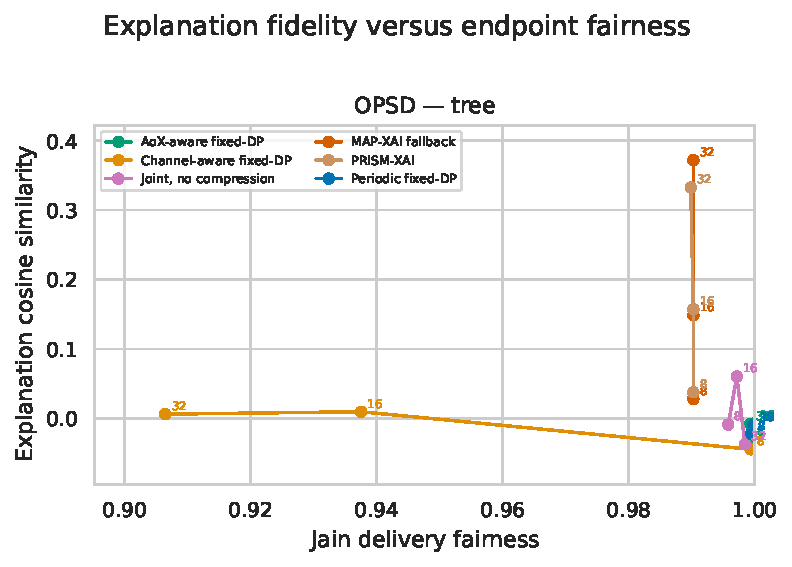
\includegraphics[width=.96\textwidth,height=.82\textheight,keepaspectratio]{../../SERVICE_TRADEOFF_RESULTS/runs/thr_3_cap_8/opsd/fairness_reliability.pdf}

\caption{Public-score threshold $\tau=3$, release cap $M=8$, OPSD: fairness--reliability plane. This panel should be read with the setting-level quantitative interpretation and the complete tables immediately preceding the figure block.}

\end{figure*}

\clearpage

\begin{figure*}[p]

\centering

\includegraphics[width=.96\textwidth,height=.82\textheight,keepaspectratio]{../../SERVICE_TRADEOFF_RESULTS/runs/thr_3_cap_8/opsd/privacy_fidelity.pdf}

\caption{Public-score threshold $\tau=3$, release cap $M=8$, OPSD: privacy--fidelity plane. This panel should be read with the setting-level quantitative interpretation and the complete tables immediately preceding the figure block.}

\end{figure*}

\clearpage

\begin{figure*}[p]

\centering

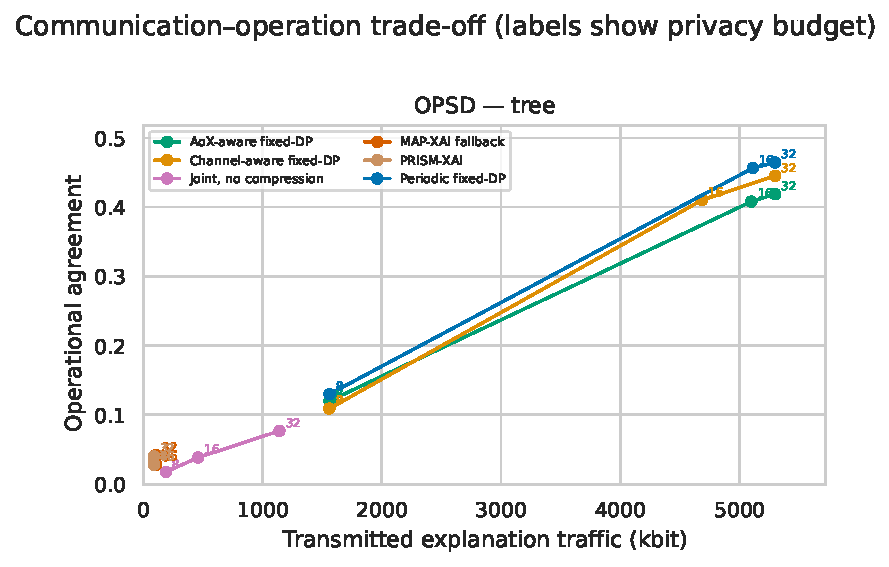
\includegraphics[width=.96\textwidth,height=.82\textheight,keepaspectratio]{../../SERVICE_TRADEOFF_RESULTS/runs/thr_3_cap_8/opsd/pareto_bits_fidelity.pdf}

\caption{Public-score threshold $\tau=3$, release cap $M=8$, OPSD: traffic--fidelity Pareto plane. This panel should be read with the setting-level quantitative interpretation and the complete tables immediately preceding the figure block.}

\end{figure*}

\clearpage

\begin{figure*}[p]

\centering

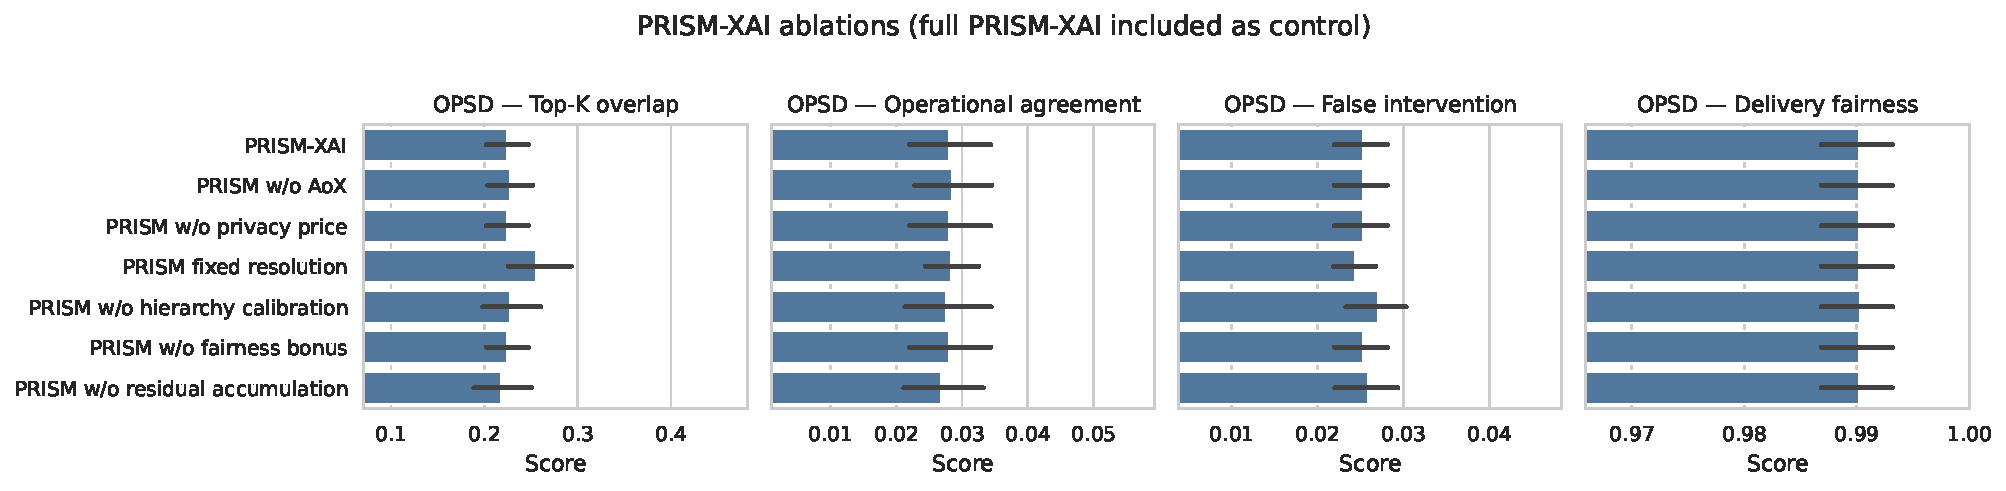
\includegraphics[width=.96\textwidth,height=.82\textheight,keepaspectratio]{../../SERVICE_TRADEOFF_RESULTS/runs/thr_3_cap_8/opsd/ablation_results.pdf}

\caption{Public-score threshold $\tau=3$, release cap $M=8$, OPSD: component ablation. This panel should be read with the setting-level quantitative interpretation and the complete tables immediately preceding the figure block.}

\end{figure*}

\clearpage

\paragraph{UCI.} The three generated tables below report the full method means, all condition-level values, and paired differences. The five figures that follow provide the corresponding temporal, fairness, privacy, Pareto, and ablation views. Aggregate panels support the setting-level summary above; dataset panels reveal whether that summary is shared by OPSD and UCI rather than being driven by their different endpoint counts.

\begin{table*}[p]\centering\tiny

\caption{Public-score threshold $\tau=3$, release cap $M=8$, UCI: complete generated method table.}

\label{tab:thr_3_cap_8:uci:main}

\resizebox{\linewidth}{!}{% Values are means with 95% Student-t confidence intervals across seeds.
\begin{tabular}{lccccccccccccccc}
\toprule
Dataset & Model & $\epsilon_{\max}$ & Method & Top-$K$ & Cosine & Decision & Recall & Prec. & Abst. & P95 ms & kbit & Spent $\epsilon$ & False int. & bit/correct & Fairness \\
\midrule
UCI & Tree & 8 & AoX-aware fixed-DP & 0.263 $\pm$ 0.041 & -0.007 $\pm$ 0.009 & 0.457 $\pm$ 0.031 & 0.457 $\pm$ 0.031 & 0.362 $\pm$ 0.024 & 0.003 $\pm$ 0.001 & 7.500 $\pm$ 0.000 & 5300.224 $\pm$ 0.000 & 7.990 $\pm$ 0.000 & 0.557 $\pm$ 0.025 & 14002.896 $\pm$ 1040.243 & 0.999 $\pm$ 0.000 \\
UCI & Tree & 8 & AoX-aware fixed-DP & 0.260 $\pm$ 0.022 & 0.010 $\pm$ 0.055 & 0.455 $\pm$ 0.047 & 0.455 $\pm$ 0.047 & 0.361 $\pm$ 0.038 & 0.003 $\pm$ 0.001 & 7.500 $\pm$ 0.000 & 5300.224 $\pm$ 0.000 & 7.990 $\pm$ 0.000 & 0.557 $\pm$ 0.048 & 14198.303 $\pm$ 1508.274 & 0.999 $\pm$ 0.000 \\
UCI & Tree & 8 & Channel-aware fixed-DP & 0.248 $\pm$ 0.031 & 0.004 $\pm$ 0.012 & 0.001 $\pm$ 0.001 & 0.001 $\pm$ 0.001 & 0.150 $\pm$ 0.151 & 0.999 $\pm$ 0.001 & 4.609 $\pm$ 1.781 & 5295.177 $\pm$ 3.740 & 7.990 $\pm$ 0.000 & 0.001 $\pm$ 0.001 & 4632196.500 $\pm$ 2102650.252 & 0.991 $\pm$ 0.001 \\
UCI & Tree & 8 & Channel-aware fixed-DP & 0.239 $\pm$ 0.030 & -0.020 $\pm$ 0.055 & 0.000 $\pm$ 0.000 & 0.000 $\pm$ 0.000 & 0.117 $\pm$ 0.225 & 0.999 $\pm$ 0.001 & 4.609 $\pm$ 1.781 & 5295.177 $\pm$ 3.740 & 7.990 $\pm$ 0.000 & 0.001 $\pm$ 0.001 & 5296989.000 $\pm$ 41104.572 & 0.991 $\pm$ 0.001 \\
UCI & Tree & 8 & Joint, no compression & 0.286 $\pm$ 0.045 & 0.004 $\pm$ 0.020 & 0.052 $\pm$ 0.005 & 0.052 $\pm$ 0.005 & 0.406 $\pm$ 0.037 & 0.875 $\pm$ 0.003 & 5.123 $\pm$ 1.792 & 672.300 $\pm$ 0.452 & 7.990 $\pm$ 0.000 & 0.053 $\pm$ 0.004 & 15676.175 $\pm$ 1475.621 & 0.994 $\pm$ 0.003 \\
UCI & Tree & 8 & Joint, no compression & 0.229 $\pm$ 0.052 & -0.032 $\pm$ 0.050 & 0.057 $\pm$ 0.007 & 0.057 $\pm$ 0.007 & 0.428 $\pm$ 0.041 & 0.875 $\pm$ 0.003 & 5.131 $\pm$ 1.787 & 672.300 $\pm$ 0.452 & 7.990 $\pm$ 0.000 & 0.052 $\pm$ 0.004 & 14702.786 $\pm$ 2334.488 & 0.994 $\pm$ 0.003 \\
UCI & Tree & 8 & Periodic fixed-DP & 0.259 $\pm$ 0.060 & -0.005 $\pm$ 0.008 & 0.006 $\pm$ 0.001 & 0.006 $\pm$ 0.001 & 0.244 $\pm$ 0.049 & 0.989 $\pm$ 0.001 & 4.596 $\pm$ 1.788 & 5299.318 $\pm$ 1.451 & 7.786 $\pm$ 0.000 & 0.013 $\pm$ 0.002 & 1215103.896 $\pm$ 390671.319 & 0.999 $\pm$ 0.000 \\
UCI & Tree & 8 & Periodic fixed-DP & 0.260 $\pm$ 0.044 & 0.022 $\pm$ 0.070 & 0.005 $\pm$ 0.001 & 0.005 $\pm$ 0.001 & 0.195 $\pm$ 0.050 & 0.989 $\pm$ 0.001 & 4.596 $\pm$ 1.788 & 5299.318 $\pm$ 1.451 & 7.786 $\pm$ 0.000 & 0.015 $\pm$ 0.002 & 1555837.203 $\pm$ 955472.503 & 0.999 $\pm$ 0.000 \\
UCI & Tree & 8 & PRISM-XAI & 0.224 $\pm$ 0.051 & -0.005 $\pm$ 0.014 & 0.040 $\pm$ 0.007 & 0.040 $\pm$ 0.007 & 0.469 $\pm$ 0.065 & 0.910 $\pm$ 0.005 & 5.647 $\pm$ 1.735 & 328.571 $\pm$ 1.335 & 7.823 $\pm$ 0.000 & 0.031 $\pm$ 0.005 & 10347.978 $\pm$ 1665.157 & 0.991 $\pm$ 0.002 \\
UCI & Tree & 8 & PRISM-XAI & 0.228 $\pm$ 0.055 & -0.004 $\pm$ 0.076 & 0.044 $\pm$ 0.009 & 0.044 $\pm$ 0.009 & 0.477 $\pm$ 0.093 & 0.911 $\pm$ 0.005 & 4.164 $\pm$ 1.674 & 325.598 $\pm$ 1.298 & 7.823 $\pm$ 0.000 & 0.033 $\pm$ 0.006 & 9624.204 $\pm$ 2175.413 & 0.992 $\pm$ 0.001 \\
UCI & Tree & 8 & MAP-XAI fallback & 0.178 $\pm$ 0.062 & 0.011 $\pm$ 0.013 & 0.040 $\pm$ 0.005 & 0.040 $\pm$ 0.005 & 0.458 $\pm$ 0.054 & 0.910 $\pm$ 0.005 & 5.670 $\pm$ 1.711 & 381.640 $\pm$ 0.105 & 7.823 $\pm$ 0.000 & 0.033 $\pm$ 0.004 & 11809.010 $\pm$ 1479.313 & 0.991 $\pm$ 0.002 \\
UCI & Tree & 8 & MAP-XAI fallback & 0.211 $\pm$ 0.046 & 0.055 $\pm$ 0.046 & 0.048 $\pm$ 0.009 & 0.048 $\pm$ 0.009 & 0.519 $\pm$ 0.078 & 0.910 $\pm$ 0.005 & 5.202 $\pm$ 1.753 & 381.153 $\pm$ 0.449 & 7.823 $\pm$ 0.000 & 0.031 $\pm$ 0.005 & 10053.490 $\pm$ 2134.182 & 0.992 $\pm$ 0.002 \\
\bottomrule
\end{tabular}
}

\end{table*}\clearpage

\begin{table*}[p]\centering\tiny

\caption{Public-score threshold $\tau=3$, release cap $M=8$, UCI: complete condition-level generated table.}

\label{tab:thr_3_cap_8:uci:conditions}

\resizebox{\textwidth}{!}{\begin{tabular}{llllccccccccccc}
\toprule
Dataset & Model & $\epsilon_{\max}$ & Method & kbit & Top-$K$ & Random Top-$K$ & Cosine & Decision & Recall & Precision & Coverage & Abstain & False int. & Spent $\epsilon$ \\
\midrule
UCI & Tree & 8 & Joint, no compression & 672.300 $\pm$ 0.452 & 0.286 $\pm$ 0.045 & 0.250 $\pm$ 0.000 & 0.004 $\pm$ 0.020 & 0.052 $\pm$ 0.005 & 0.052 $\pm$ 0.005 & 0.406 $\pm$ 0.037 & 0.125 $\pm$ 0.003 & 0.875 $\pm$ 0.003 & 0.053 $\pm$ 0.004 & 7.990 $\pm$ 0.000 \\
UCI & Tree & 8 & Joint, no compression & 672.300 $\pm$ 0.452 & 0.229 $\pm$ 0.052 & 0.250 $\pm$ 0.000 & -0.032 $\pm$ 0.050 & 0.057 $\pm$ 0.007 & 0.057 $\pm$ 0.007 & 0.428 $\pm$ 0.041 & 0.125 $\pm$ 0.003 & 0.875 $\pm$ 0.003 & 0.052 $\pm$ 0.004 & 7.990 $\pm$ 0.000 \\
UCI & Tree & 8 & Periodic fixed-DP & 5299.318 $\pm$ 1.451 & 0.259 $\pm$ 0.060 & 0.250 $\pm$ 0.000 & -0.005 $\pm$ 0.008 & 0.006 $\pm$ 0.001 & 0.006 $\pm$ 0.001 & 0.244 $\pm$ 0.049 & 0.011 $\pm$ 0.001 & 0.989 $\pm$ 0.001 & 0.013 $\pm$ 0.002 & 7.786 $\pm$ 0.000 \\
UCI & Tree & 8 & Periodic fixed-DP & 5299.318 $\pm$ 1.451 & 0.260 $\pm$ 0.044 & 0.250 $\pm$ 0.000 & 0.022 $\pm$ 0.070 & 0.005 $\pm$ 0.001 & 0.005 $\pm$ 0.001 & 0.195 $\pm$ 0.050 & 0.011 $\pm$ 0.001 & 0.989 $\pm$ 0.001 & 0.015 $\pm$ 0.002 & 7.786 $\pm$ 0.000 \\
UCI & Tree & 8 & PRISM-XAI & 328.571 $\pm$ 1.335 & 0.224 $\pm$ 0.051 & 0.250 $\pm$ 0.000 & -0.005 $\pm$ 0.014 & 0.040 $\pm$ 0.007 & 0.040 $\pm$ 0.007 & 0.469 $\pm$ 0.065 & 0.090 $\pm$ 0.005 & 0.910 $\pm$ 0.005 & 0.031 $\pm$ 0.005 & 7.823 $\pm$ 0.000 \\
UCI & Tree & 8 & PRISM-XAI & 325.598 $\pm$ 1.298 & 0.228 $\pm$ 0.055 & 0.250 $\pm$ 0.000 & -0.004 $\pm$ 0.076 & 0.044 $\pm$ 0.009 & 0.044 $\pm$ 0.009 & 0.477 $\pm$ 0.093 & 0.089 $\pm$ 0.005 & 0.911 $\pm$ 0.005 & 0.033 $\pm$ 0.006 & 7.823 $\pm$ 0.000 \\
UCI & Tree & 16 & Joint, no compression & 1632.150 $\pm$ 0.339 & 0.216 $\pm$ 0.041 & 0.250 $\pm$ 0.000 & 0.001 $\pm$ 0.012 & 0.094 $\pm$ 0.005 & 0.094 $\pm$ 0.005 & 0.330 $\pm$ 0.024 & 0.228 $\pm$ 0.005 & 0.772 $\pm$ 0.005 & 0.133 $\pm$ 0.010 & 15.997 $\pm$ 0.000 \\
UCI & Tree & 16 & Joint, no compression & 1632.600 $\pm$ 0.554 & 0.204 $\pm$ 0.011 & 0.250 $\pm$ 0.000 & -0.021 $\pm$ 0.033 & 0.099 $\pm$ 0.016 & 0.099 $\pm$ 0.016 & 0.347 $\pm$ 0.054 & 0.228 $\pm$ 0.005 & 0.772 $\pm$ 0.005 & 0.128 $\pm$ 0.011 & 15.997 $\pm$ 0.000 \\
UCI & Tree & 16 & Periodic fixed-DP & 5299.318 $\pm$ 1.451 & 0.259 $\pm$ 0.060 & 0.250 $\pm$ 0.000 & -0.005 $\pm$ 0.008 & 0.006 $\pm$ 0.001 & 0.006 $\pm$ 0.001 & 0.244 $\pm$ 0.049 & 0.011 $\pm$ 0.001 & 0.989 $\pm$ 0.001 & 0.013 $\pm$ 0.002 & 7.786 $\pm$ 0.000 \\
UCI & Tree & 16 & Periodic fixed-DP & 5299.318 $\pm$ 1.451 & 0.260 $\pm$ 0.044 & 0.250 $\pm$ 0.000 & 0.022 $\pm$ 0.070 & 0.005 $\pm$ 0.001 & 0.005 $\pm$ 0.001 & 0.195 $\pm$ 0.050 & 0.011 $\pm$ 0.001 & 0.989 $\pm$ 0.001 & 0.015 $\pm$ 0.002 & 7.786 $\pm$ 0.000 \\
UCI & Tree & 16 & PRISM-XAI & 327.906 $\pm$ 1.114 & 0.246 $\pm$ 0.072 & 0.250 $\pm$ 0.000 & 0.001 $\pm$ 0.014 & 0.043 $\pm$ 0.005 & 0.043 $\pm$ 0.005 & 0.544 $\pm$ 0.057 & 0.090 $\pm$ 0.005 & 0.910 $\pm$ 0.005 & 0.025 $\pm$ 0.004 & 15.620 $\pm$ 0.000 \\
UCI & Tree & 16 & PRISM-XAI & 324.636 $\pm$ 1.010 & 0.225 $\pm$ 0.054 & 0.250 $\pm$ 0.000 & -0.001 $\pm$ 0.073 & 0.043 $\pm$ 0.008 & 0.043 $\pm$ 0.008 & 0.586 $\pm$ 0.085 & 0.084 $\pm$ 0.004 & 0.916 $\pm$ 0.004 & 0.021 $\pm$ 0.005 & 15.620 $\pm$ 0.000 \\
UCI & Tree & 32 & Joint, no compression & 4034.550 $\pm$ 5.034 & 0.246 $\pm$ 0.031 & 0.250 $\pm$ 0.000 & -0.002 $\pm$ 0.015 & 0.228 $\pm$ 0.013 & 0.228 $\pm$ 0.013 & 0.361 $\pm$ 0.028 & 0.537 $\pm$ 0.009 & 0.463 $\pm$ 0.009 & 0.279 $\pm$ 0.017 & 31.999 $\pm$ 0.000 \\
UCI & Tree & 32 & Joint, no compression & 4034.550 $\pm$ 5.034 & 0.241 $\pm$ 0.033 & 0.250 $\pm$ 0.000 & -0.012 $\pm$ 0.030 & 0.228 $\pm$ 0.028 & 0.228 $\pm$ 0.028 & 0.360 $\pm$ 0.047 & 0.530 $\pm$ 0.010 & 0.470 $\pm$ 0.010 & 0.280 $\pm$ 0.026 & 31.999 $\pm$ 0.000 \\
UCI & Tree & 32 & Periodic fixed-DP & 5299.318 $\pm$ 1.451 & 0.259 $\pm$ 0.060 & 0.250 $\pm$ 0.000 & -0.005 $\pm$ 0.008 & 0.006 $\pm$ 0.001 & 0.006 $\pm$ 0.001 & 0.244 $\pm$ 0.049 & 0.011 $\pm$ 0.001 & 0.989 $\pm$ 0.001 & 0.013 $\pm$ 0.002 & 7.786 $\pm$ 0.000 \\
UCI & Tree & 32 & Periodic fixed-DP & 5299.318 $\pm$ 1.451 & 0.260 $\pm$ 0.044 & 0.250 $\pm$ 0.000 & 0.022 $\pm$ 0.070 & 0.005 $\pm$ 0.001 & 0.005 $\pm$ 0.001 & 0.195 $\pm$ 0.050 & 0.011 $\pm$ 0.001 & 0.989 $\pm$ 0.001 & 0.015 $\pm$ 0.002 & 7.786 $\pm$ 0.000 \\
UCI & Tree & 32 & PRISM-XAI & 328.131 $\pm$ 1.290 & 0.274 $\pm$ 0.061 & 0.250 $\pm$ 0.000 & 0.011 $\pm$ 0.017 & 0.038 $\pm$ 0.004 & 0.038 $\pm$ 0.004 & 0.873 $\pm$ 0.070 & 0.083 $\pm$ 0.003 & 0.917 $\pm$ 0.003 & 0.004 $\pm$ 0.003 & 31.175 $\pm$ 0.000 \\
UCI & Tree & 32 & PRISM-XAI & 324.963 $\pm$ 1.575 & 0.273 $\pm$ 0.067 & 0.250 $\pm$ 0.000 & 0.016 $\pm$ 0.096 & 0.037 $\pm$ 0.005 & 0.037 $\pm$ 0.005 & 0.936 $\pm$ 0.069 & 0.073 $\pm$ 0.003 & 0.927 $\pm$ 0.003 & 0.002 $\pm$ 0.003 & 31.175 $\pm$ 0.000 \\
\bottomrule
\end{tabular}
}

\end{table*}\clearpage

\begin{table*}[p]\centering\tiny

\caption{Public-score threshold $\tau=3$, release cap $M=8$, UCI: complete generated paired comparisons.}

\label{tab:thr_3_cap_8:uci:paired}

\resizebox{\textwidth}{!}{\begin{tabular}{llcccc}
\toprule
Dataset & Baseline & Delta kbit & Delta Top-$K$ & Delta recall & Delta fairness \\
\midrule
UCI & AoX-aware fixed-DP & -4971.653 $\pm$ 1.335 & -0.039 $\pm$ 0.084 & -0.417 $\pm$ 0.031 & -0.009 $\pm$ 0.002 \\
UCI & AoX-aware fixed-DP & -4972.318 $\pm$ 1.114 & -0.018 $\pm$ 0.091 & -0.415 $\pm$ 0.030 & -0.008 $\pm$ 0.002 \\
UCI & AoX-aware fixed-DP & -4972.093 $\pm$ 1.290 & 0.010 $\pm$ 0.061 & -0.419 $\pm$ 0.032 & -0.008 $\pm$ 0.002 \\
UCI & AoX-aware fixed-DP & -4974.626 $\pm$ 1.298 & -0.032 $\pm$ 0.056 & -0.411 $\pm$ 0.049 & -0.007 $\pm$ 0.001 \\
UCI & AoX-aware fixed-DP & -4975.588 $\pm$ 1.010 & -0.035 $\pm$ 0.047 & -0.411 $\pm$ 0.047 & -0.006 $\pm$ 0.002 \\
UCI & AoX-aware fixed-DP & -4975.261 $\pm$ 1.575 & 0.013 $\pm$ 0.058 & -0.417 $\pm$ 0.047 & -0.006 $\pm$ 0.002 \\
UCI & Channel-aware fixed-DP & -4966.606 $\pm$ 3.827 & -0.024 $\pm$ 0.060 & 0.039 $\pm$ 0.006 & -0.000 $\pm$ 0.002 \\
UCI & Channel-aware fixed-DP & -4972.318 $\pm$ 1.114 & -0.022 $\pm$ 0.079 & 0.042 $\pm$ 0.005 & 0.661 $\pm$ 0.002 \\
UCI & Channel-aware fixed-DP & -4972.093 $\pm$ 1.290 & 0.006 $\pm$ 0.063 & 0.037 $\pm$ 0.005 & 0.736 $\pm$ 0.002 \\
UCI & Channel-aware fixed-DP & -4969.580 $\pm$ 4.222 & -0.011 $\pm$ 0.068 & 0.044 $\pm$ 0.010 & 0.001 $\pm$ 0.001 \\
UCI & Channel-aware fixed-DP & -4975.588 $\pm$ 1.010 & -0.035 $\pm$ 0.050 & 0.043 $\pm$ 0.008 & 0.662 $\pm$ 0.002 \\
UCI & Channel-aware fixed-DP & -4975.261 $\pm$ 1.575 & 0.014 $\pm$ 0.069 & 0.037 $\pm$ 0.005 & 0.738 $\pm$ 0.003 \\
UCI & Joint, no compression & -343.729 $\pm$ 1.578 & -0.061 $\pm$ 0.086 & -0.012 $\pm$ 0.008 & -0.003 $\pm$ 0.003 \\
UCI & Joint, no compression & -1304.244 $\pm$ 1.271 & 0.029 $\pm$ 0.092 & -0.052 $\pm$ 0.006 & -0.006 $\pm$ 0.002 \\
UCI & Joint, no compression & -3706.419 $\pm$ 4.695 & 0.028 $\pm$ 0.058 & -0.190 $\pm$ 0.013 & -0.007 $\pm$ 0.002 \\
UCI & Joint, no compression & -346.702 $\pm$ 1.528 & -0.002 $\pm$ 0.075 & -0.013 $\pm$ 0.012 & -0.002 $\pm$ 0.003 \\
UCI & Joint, no compression & -1307.964 $\pm$ 0.799 & 0.021 $\pm$ 0.051 & -0.056 $\pm$ 0.018 & -0.005 $\pm$ 0.002 \\
UCI & Joint, no compression & -3709.587 $\pm$ 5.063 & 0.032 $\pm$ 0.078 & -0.191 $\pm$ 0.030 & -0.006 $\pm$ 0.002 \\
UCI & Periodic fixed-DP & -4970.747 $\pm$ 1.956 & -0.035 $\pm$ 0.082 & 0.034 $\pm$ 0.007 & -0.009 $\pm$ 0.002 \\
UCI & Periodic fixed-DP & -4971.412 $\pm$ 1.872 & -0.014 $\pm$ 0.077 & 0.037 $\pm$ 0.006 & -0.008 $\pm$ 0.002 \\
UCI & Periodic fixed-DP & -4971.187 $\pm$ 1.698 & 0.015 $\pm$ 0.099 & 0.032 $\pm$ 0.004 & -0.008 $\pm$ 0.002 \\
UCI & Periodic fixed-DP & -4973.721 $\pm$ 1.578 & -0.033 $\pm$ 0.093 & 0.039 $\pm$ 0.008 & -0.007 $\pm$ 0.002 \\
UCI & Periodic fixed-DP & -4974.682 $\pm$ 1.543 & -0.035 $\pm$ 0.074 & 0.038 $\pm$ 0.007 & -0.007 $\pm$ 0.002 \\
UCI & Periodic fixed-DP & -4974.355 $\pm$ 1.546 & 0.013 $\pm$ 0.096 & 0.032 $\pm$ 0.005 & -0.006 $\pm$ 0.002 \\
UCI & MAP-XAI fallback & -53.069 $\pm$ 1.324 & 0.047 $\pm$ 0.064 & 0.000 $\pm$ 0.005 & 0.000 $\pm$ 0.000 \\
UCI & MAP-XAI fallback & -53.673 $\pm$ 1.109 & 0.023 $\pm$ 0.057 & 0.001 $\pm$ 0.004 & -0.000 $\pm$ 0.001 \\
UCI & MAP-XAI fallback & -53.427 $\pm$ 1.194 & 0.041 $\pm$ 0.046 & -0.004 $\pm$ 0.004 & -0.000 $\pm$ 0.001 \\
UCI & MAP-XAI fallback & -55.556 $\pm$ 1.430 & 0.017 $\pm$ 0.054 & -0.004 $\pm$ 0.007 & 0.000 $\pm$ 0.000 \\
UCI & MAP-XAI fallback & -56.375 $\pm$ 1.113 & -0.005 $\pm$ 0.048 & 0.001 $\pm$ 0.007 & 0.001 $\pm$ 0.002 \\
UCI & MAP-XAI fallback & -55.666 $\pm$ 1.169 & -0.026 $\pm$ 0.079 & -0.001 $\pm$ 0.006 & 0.000 $\pm$ 0.001 \\
\bottomrule
\end{tabular}
}

\end{table*}\clearpage

\begin{figure*}[p]

\centering

\includegraphics[width=.96\textwidth,height=.82\textheight,keepaspectratio]{../../SERVICE_TRADEOFF_RESULTS/runs/thr_3_cap_8/uci/regime_trace.pdf}

\caption{Public-score threshold $\tau=3$, release cap $M=8$, UCI: representative regime trace. This panel should be read with the setting-level quantitative interpretation and the complete tables immediately preceding the figure block.}

\end{figure*}

\clearpage

\begin{figure*}[p]

\centering

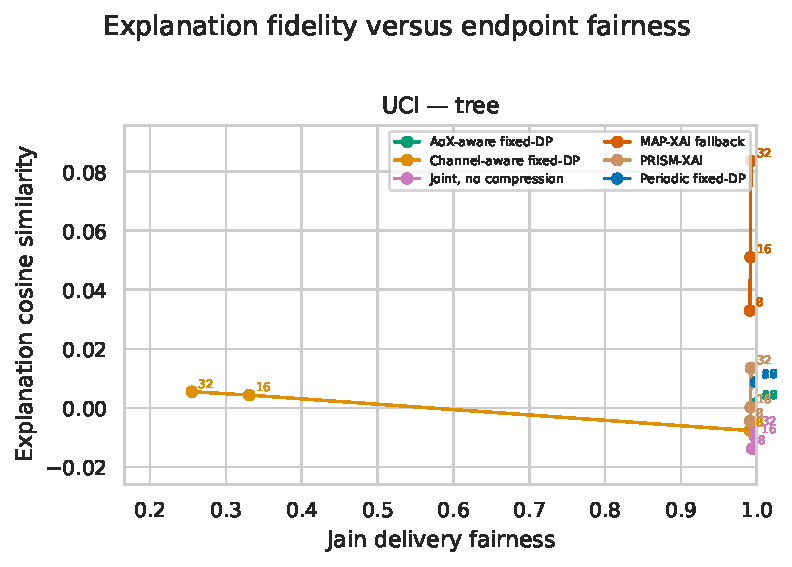
\includegraphics[width=.96\textwidth,height=.82\textheight,keepaspectratio]{../../SERVICE_TRADEOFF_RESULTS/runs/thr_3_cap_8/uci/fairness_reliability.pdf}

\caption{Public-score threshold $\tau=3$, release cap $M=8$, UCI: fairness--reliability plane. This panel should be read with the setting-level quantitative interpretation and the complete tables immediately preceding the figure block.}

\end{figure*}

\clearpage

\begin{figure*}[p]

\centering

\includegraphics[width=.96\textwidth,height=.82\textheight,keepaspectratio]{../../SERVICE_TRADEOFF_RESULTS/runs/thr_3_cap_8/uci/privacy_fidelity.pdf}

\caption{Public-score threshold $\tau=3$, release cap $M=8$, UCI: privacy--fidelity plane. This panel should be read with the setting-level quantitative interpretation and the complete tables immediately preceding the figure block.}

\end{figure*}

\clearpage

\begin{figure*}[p]

\centering

\includegraphics[width=.96\textwidth,height=.82\textheight,keepaspectratio]{../../SERVICE_TRADEOFF_RESULTS/runs/thr_3_cap_8/uci/pareto_bits_fidelity.pdf}

\caption{Public-score threshold $\tau=3$, release cap $M=8$, UCI: traffic--fidelity Pareto plane. This panel should be read with the setting-level quantitative interpretation and the complete tables immediately preceding the figure block.}

\end{figure*}

\clearpage

\begin{figure*}[p]

\centering

\includegraphics[width=.96\textwidth,height=.82\textheight,keepaspectratio]{../../SERVICE_TRADEOFF_RESULTS/runs/thr_3_cap_8/uci/ablation_results.pdf}

\caption{Public-score threshold $\tau=3$, release cap $M=8$, UCI: component ablation. This panel should be read with the setting-level quantitative interpretation and the complete tables immediately preceding the figure block.}

\end{figure*}

\clearpage

\subsubsection{Public-score threshold $\tau=1$, release cap $M=16$}

At this operating point, PRISM-XAI transmits 342.50~kbit versus 407.81~kbit for MAP-XAI-only (aggregate-mean ratio saving 16.01\%). The paired difference is -65.31$\pm$7.13~kbit. PRISM coverage is 0.0856, critical-event recall is 0.0401, and maximum recorded expenditure is 17.727. Relative to MAP-XAI-only, the paired coverage change is -0.00075$\pm$0.00093 and recall change is +0.00082$\pm$0.00162. The descriptive overlap rule holds in 8 of 12 cells. Accordingly, this point is read as a sensitivity point on the service frontier, not a complete matched-service confirmation.

\paragraph{Combined datasets.} The three generated tables below report the full method means, all condition-level values, and paired differences. The five figures that follow provide the corresponding temporal, fairness, privacy, Pareto, and ablation views. Aggregate panels support the setting-level summary above; dataset panels reveal whether that summary is shared by OPSD and UCI rather than being driven by their different endpoint counts.

\begin{table*}[p]\centering\tiny

\caption{Public-score threshold $\tau=1$, release cap $M=16$, Combined datasets: complete generated method table.}

\label{tab:thr_1_cap_16:combined:main}

\resizebox{\linewidth}{!}{% Values are means with 95% Student-t confidence intervals across seeds.
\begin{tabular}{lccccccccccccccc}
\toprule
Dataset & Model & $\epsilon_{\max}$ & Method & Top-$K$ & Cosine & Decision & Recall & Prec. & Abst. & P95 ms & kbit & Spent $\epsilon$ & False int. & bit/correct & Fairness \\
\midrule
OPSD & Tree & 8 & AoX-aware fixed-DP & 0.234 $\pm$ 0.048 & -0.033 $\pm$ 0.028 & 0.119 $\pm$ 0.028 & 0.119 $\pm$ 0.028 & 0.198 $\pm$ 0.054 & 0.721 $\pm$ 0.005 & 6.903 $\pm$ 1.126 & 1560.564 $\pm$ 0.000 & 7.990 $\pm$ 0.000 & 0.183 $\pm$ 0.020 & 35567.482 $\pm$ 10569.818 & 0.999 $\pm$ 0.000 \\
OPSD & Tree & 8 & AoX-aware fixed-DP & 0.238 $\pm$ 0.049 & -0.026 $\pm$ 0.055 & 0.121 $\pm$ 0.026 & 0.121 $\pm$ 0.026 & 0.205 $\pm$ 0.053 & 0.721 $\pm$ 0.005 & 6.903 $\pm$ 1.126 & 1560.564 $\pm$ 0.000 & 7.990 $\pm$ 0.000 & 0.179 $\pm$ 0.023 & 34123.214 $\pm$ 8376.542 & 0.999 $\pm$ 0.000 \\
OPSD & Tree & 8 & Channel-aware fixed-DP & 0.292 $\pm$ 0.037 & -0.041 $\pm$ 0.051 & 0.107 $\pm$ 0.026 & 0.107 $\pm$ 0.026 & 0.217 $\pm$ 0.068 & 0.779 $\pm$ 0.011 & 5.571 $\pm$ 1.784 & 1560.564 $\pm$ 0.000 & 7.990 $\pm$ 0.000 & 0.154 $\pm$ 0.029 & 40860.756 $\pm$ 14126.920 & 0.999 $\pm$ 0.000 \\
OPSD & Tree & 8 & Channel-aware fixed-DP & 0.292 $\pm$ 0.054 & -0.049 $\pm$ 0.064 & 0.111 $\pm$ 0.023 & 0.111 $\pm$ 0.023 & 0.228 $\pm$ 0.066 & 0.779 $\pm$ 0.011 & 5.571 $\pm$ 1.784 & 1560.564 $\pm$ 0.000 & 7.990 $\pm$ 0.000 & 0.149 $\pm$ 0.026 & 37980.855 $\pm$ 12338.094 & 0.999 $\pm$ 0.000 \\
OPSD & Tree & 8 & Joint, no compression & 0.288 $\pm$ 0.064 & -0.030 $\pm$ 0.079 & 0.016 $\pm$ 0.005 & 0.016 $\pm$ 0.005 & 0.193 $\pm$ 0.059 & 0.957 $\pm$ 0.003 & 4.560 $\pm$ 1.811 & 189.900 $\pm$ 0.554 & 7.990 $\pm$ 0.000 & 0.027 $\pm$ 0.005 & 32490.357 $\pm$ 10149.755 & 0.996 $\pm$ 0.002 \\
OPSD & Tree & 8 & Joint, no compression & 0.258 $\pm$ 0.055 & 0.011 $\pm$ 0.094 & 0.019 $\pm$ 0.004 & 0.019 $\pm$ 0.004 & 0.224 $\pm$ 0.044 & 0.957 $\pm$ 0.003 & 4.562 $\pm$ 1.809 & 189.750 $\pm$ 0.566 & 7.990 $\pm$ 0.000 & 0.025 $\pm$ 0.003 & 26079.167 $\pm$ 6335.386 & 0.996 $\pm$ 0.002 \\
OPSD & Tree & 8 & Periodic fixed-DP & 0.241 $\pm$ 0.049 & -0.019 $\pm$ 0.061 & 0.125 $\pm$ 0.020 & 0.125 $\pm$ 0.020 & 0.209 $\pm$ 0.044 & 0.722 $\pm$ 0.006 & 6.303 $\pm$ 1.438 & 1560.564 $\pm$ 0.000 & 7.990 $\pm$ 0.000 & 0.181 $\pm$ 0.021 & 31183.082 $\pm$ 4356.378 & 0.999 $\pm$ 0.000 \\
OPSD & Tree & 8 & Periodic fixed-DP & 0.242 $\pm$ 0.048 & -0.026 $\pm$ 0.082 & 0.135 $\pm$ 0.016 & 0.135 $\pm$ 0.016 & 0.231 $\pm$ 0.037 & 0.722 $\pm$ 0.006 & 6.303 $\pm$ 1.438 & 1560.564 $\pm$ 0.000 & 7.990 $\pm$ 0.000 & 0.169 $\pm$ 0.017 & 28520.235 $\pm$ 3511.595 & 0.999 $\pm$ 0.000 \\
OPSD & Tree & 8 & PRISM-XAI & 0.270 $\pm$ 0.066 & -0.025 $\pm$ 0.093 & 0.015 $\pm$ 0.004 & 0.015 $\pm$ 0.004 & 0.200 $\pm$ 0.078 & 0.956 $\pm$ 0.003 & 4.630 $\pm$ 1.839 & 87.697 $\pm$ 0.410 & 6.034 $\pm$ 0.230 & 0.025 $\pm$ 0.005 & 15451.736 $\pm$ 3728.991 & 0.993 $\pm$ 0.004 \\
OPSD & Tree & 8 & PRISM-XAI & 0.283 $\pm$ 0.054 & -0.005 $\pm$ 0.086 & 0.017 $\pm$ 0.005 & 0.017 $\pm$ 0.005 & 0.222 $\pm$ 0.080 & 0.956 $\pm$ 0.003 & 4.630 $\pm$ 1.839 & 87.431 $\pm$ 0.364 & 5.936 $\pm$ 0.213 & 0.024 $\pm$ 0.005 & 14279.307 $\pm$ 3768.065 & 0.993 $\pm$ 0.004 \\
OPSD & Tree & 8 & MAP-XAI fallback & 0.234 $\pm$ 0.073 & -0.037 $\pm$ 0.075 & 0.016 $\pm$ 0.005 & 0.016 $\pm$ 0.005 & 0.191 $\pm$ 0.080 & 0.956 $\pm$ 0.003 & 4.732 $\pm$ 1.776 & 105.817 $\pm$ 0.049 & 7.786 $\pm$ 0.000 & 0.027 $\pm$ 0.006 & 21385.963 $\pm$ 9729.377 & 0.993 $\pm$ 0.004 \\
OPSD & Tree & 8 & MAP-XAI fallback & 0.230 $\pm$ 0.067 & -0.012 $\pm$ 0.085 & 0.017 $\pm$ 0.005 & 0.017 $\pm$ 0.005 & 0.219 $\pm$ 0.073 & 0.956 $\pm$ 0.003 & 4.732 $\pm$ 1.776 & 105.675 $\pm$ 0.049 & 7.786 $\pm$ 0.000 & 0.024 $\pm$ 0.006 & 19083.433 $\pm$ 9057.454 & 0.993 $\pm$ 0.004 \\
UCI & Tree & 8 & AoX-aware fixed-DP & 0.263 $\pm$ 0.041 & -0.007 $\pm$ 0.009 & 0.457 $\pm$ 0.031 & 0.457 $\pm$ 0.031 & 0.362 $\pm$ 0.024 & 0.003 $\pm$ 0.001 & 7.500 $\pm$ 0.000 & 5300.224 $\pm$ 0.000 & 7.990 $\pm$ 0.000 & 0.557 $\pm$ 0.025 & 14002.896 $\pm$ 1040.243 & 0.999 $\pm$ 0.000 \\
UCI & Tree & 8 & AoX-aware fixed-DP & 0.260 $\pm$ 0.022 & 0.010 $\pm$ 0.055 & 0.455 $\pm$ 0.047 & 0.455 $\pm$ 0.047 & 0.361 $\pm$ 0.038 & 0.003 $\pm$ 0.001 & 7.500 $\pm$ 0.000 & 5300.224 $\pm$ 0.000 & 7.990 $\pm$ 0.000 & 0.557 $\pm$ 0.048 & 14198.303 $\pm$ 1508.274 & 0.999 $\pm$ 0.000 \\
UCI & Tree & 8 & Channel-aware fixed-DP & 0.248 $\pm$ 0.031 & 0.004 $\pm$ 0.012 & 0.001 $\pm$ 0.001 & 0.001 $\pm$ 0.001 & 0.150 $\pm$ 0.151 & 0.999 $\pm$ 0.001 & 4.609 $\pm$ 1.781 & 5295.177 $\pm$ 3.740 & 7.990 $\pm$ 0.000 & 0.001 $\pm$ 0.001 & 4632196.500 $\pm$ 2102650.252 & 0.991 $\pm$ 0.001 \\
UCI & Tree & 8 & Channel-aware fixed-DP & 0.239 $\pm$ 0.030 & -0.020 $\pm$ 0.055 & 0.000 $\pm$ 0.000 & 0.000 $\pm$ 0.000 & 0.117 $\pm$ 0.225 & 0.999 $\pm$ 0.001 & 4.609 $\pm$ 1.781 & 5295.177 $\pm$ 3.740 & 7.990 $\pm$ 0.000 & 0.001 $\pm$ 0.001 & 5296989.000 $\pm$ 41104.572 & 0.991 $\pm$ 0.001 \\
UCI & Tree & 8 & Joint, no compression & 0.286 $\pm$ 0.045 & 0.004 $\pm$ 0.020 & 0.052 $\pm$ 0.005 & 0.052 $\pm$ 0.005 & 0.406 $\pm$ 0.037 & 0.875 $\pm$ 0.003 & 5.123 $\pm$ 1.792 & 672.300 $\pm$ 0.452 & 7.990 $\pm$ 0.000 & 0.053 $\pm$ 0.004 & 15676.175 $\pm$ 1475.621 & 0.994 $\pm$ 0.003 \\
UCI & Tree & 8 & Joint, no compression & 0.229 $\pm$ 0.052 & -0.032 $\pm$ 0.050 & 0.057 $\pm$ 0.007 & 0.057 $\pm$ 0.007 & 0.428 $\pm$ 0.041 & 0.875 $\pm$ 0.003 & 5.131 $\pm$ 1.787 & 672.300 $\pm$ 0.452 & 7.990 $\pm$ 0.000 & 0.052 $\pm$ 0.004 & 14702.786 $\pm$ 2334.488 & 0.994 $\pm$ 0.003 \\
UCI & Tree & 8 & Periodic fixed-DP & 0.259 $\pm$ 0.060 & -0.005 $\pm$ 0.008 & 0.006 $\pm$ 0.001 & 0.006 $\pm$ 0.001 & 0.244 $\pm$ 0.049 & 0.989 $\pm$ 0.001 & 4.596 $\pm$ 1.788 & 5299.318 $\pm$ 1.451 & 7.786 $\pm$ 0.000 & 0.013 $\pm$ 0.002 & 1215103.896 $\pm$ 390671.319 & 0.999 $\pm$ 0.000 \\
UCI & Tree & 8 & Periodic fixed-DP & 0.260 $\pm$ 0.044 & 0.022 $\pm$ 0.070 & 0.005 $\pm$ 0.001 & 0.005 $\pm$ 0.001 & 0.195 $\pm$ 0.050 & 0.989 $\pm$ 0.001 & 4.596 $\pm$ 1.788 & 5299.318 $\pm$ 1.451 & 7.786 $\pm$ 0.000 & 0.015 $\pm$ 0.002 & 1555837.203 $\pm$ 955472.503 & 0.999 $\pm$ 0.000 \\
UCI & Tree & 8 & PRISM-XAI & 0.240 $\pm$ 0.089 & -0.008 $\pm$ 0.019 & 0.031 $\pm$ 0.004 & 0.031 $\pm$ 0.004 & 0.422 $\pm$ 0.039 & 0.931 $\pm$ 0.004 & 6.267 $\pm$ 1.448 & 323.739 $\pm$ 1.239 & 6.844 $\pm$ 0.203 & 0.030 $\pm$ 0.005 & 13090.115 $\pm$ 2761.149 & 0.990 $\pm$ 0.003 \\
UCI & Tree & 8 & PRISM-XAI & 0.264 $\pm$ 0.044 & -0.056 $\pm$ 0.057 & 0.027 $\pm$ 0.005 & 0.027 $\pm$ 0.005 & 0.404 $\pm$ 0.063 & 0.938 $\pm$ 0.003 & 4.814 $\pm$ 1.710 & 321.228 $\pm$ 1.066 & 6.726 $\pm$ 0.146 & 0.027 $\pm$ 0.004 & 15136.774 $\pm$ 2629.908 & 0.989 $\pm$ 0.006 \\
UCI & Tree & 8 & MAP-XAI fallback & 0.240 $\pm$ 0.077 & -0.011 $\pm$ 0.019 & 0.032 $\pm$ 0.005 & 0.032 $\pm$ 0.005 & 0.446 $\pm$ 0.058 & 0.931 $\pm$ 0.004 & 5.672 $\pm$ 1.709 & 382.099 $\pm$ 0.159 & 7.786 $\pm$ 0.000 & 0.027 $\pm$ 0.003 & 15488.351 $\pm$ 4957.026 & 0.991 $\pm$ 0.003 \\
UCI & Tree & 8 & MAP-XAI fallback & 0.265 $\pm$ 0.046 & -0.009 $\pm$ 0.057 & 0.029 $\pm$ 0.005 & 0.029 $\pm$ 0.005 & 0.424 $\pm$ 0.053 & 0.937 $\pm$ 0.004 & 5.276 $\pm$ 1.728 & 381.645 $\pm$ 0.090 & 7.786 $\pm$ 0.000 & 0.027 $\pm$ 0.005 & 16573.020 $\pm$ 2779.080 & 0.990 $\pm$ 0.004 \\
\bottomrule
\end{tabular}
}

\end{table*}\clearpage

\begin{table*}[p]\centering\tiny

\caption{Public-score threshold $\tau=1$, release cap $M=16$, Combined datasets: complete condition-level generated table.}

\label{tab:thr_1_cap_16:combined:conditions}

\resizebox{\textwidth}{!}{\begin{tabular}{llllccccccccccc}
\toprule
Dataset & Model & $\epsilon_{\max}$ & Method & kbit & Top-$K$ & Random Top-$K$ & Cosine & Decision & Recall & Precision & Coverage & Abstain & False int. & Spent $\epsilon$ \\
\midrule
OPSD & Tree & 8 & Joint, no compression & 189.900 $\pm$ 0.554 & 0.288 $\pm$ 0.064 & 0.250 $\pm$ 0.000 & -0.030 $\pm$ 0.079 & 0.016 $\pm$ 0.005 & 0.016 $\pm$ 0.005 & 0.193 $\pm$ 0.059 & 0.043 $\pm$ 0.003 & 0.957 $\pm$ 0.003 & 0.027 $\pm$ 0.005 & 7.990 $\pm$ 0.000 \\
OPSD & Tree & 8 & Joint, no compression & 189.750 $\pm$ 0.566 & 0.258 $\pm$ 0.055 & 0.250 $\pm$ 0.000 & 0.011 $\pm$ 0.094 & 0.019 $\pm$ 0.004 & 0.019 $\pm$ 0.004 & 0.224 $\pm$ 0.044 & 0.043 $\pm$ 0.003 & 0.957 $\pm$ 0.003 & 0.025 $\pm$ 0.003 & 7.990 $\pm$ 0.000 \\
OPSD & Tree & 8 & Periodic fixed-DP & 1560.564 $\pm$ 0.000 & 0.241 $\pm$ 0.049 & 0.250 $\pm$ 0.000 & -0.019 $\pm$ 0.061 & 0.125 $\pm$ 0.020 & 0.125 $\pm$ 0.020 & 0.209 $\pm$ 0.044 & 0.278 $\pm$ 0.006 & 0.722 $\pm$ 0.006 & 0.181 $\pm$ 0.021 & 7.990 $\pm$ 0.000 \\
OPSD & Tree & 8 & Periodic fixed-DP & 1560.564 $\pm$ 0.000 & 0.242 $\pm$ 0.048 & 0.250 $\pm$ 0.000 & -0.026 $\pm$ 0.082 & 0.135 $\pm$ 0.016 & 0.135 $\pm$ 0.016 & 0.231 $\pm$ 0.037 & 0.278 $\pm$ 0.006 & 0.722 $\pm$ 0.006 & 0.169 $\pm$ 0.017 & 7.990 $\pm$ 0.000 \\
OPSD & Tree & 8 & PRISM-XAI & 87.697 $\pm$ 0.410 & 0.270 $\pm$ 0.066 & 0.250 $\pm$ 0.000 & -0.025 $\pm$ 0.093 & 0.015 $\pm$ 0.004 & 0.015 $\pm$ 0.004 & 0.200 $\pm$ 0.078 & 0.044 $\pm$ 0.003 & 0.956 $\pm$ 0.003 & 0.025 $\pm$ 0.005 & 6.034 $\pm$ 0.230 \\
OPSD & Tree & 8 & PRISM-XAI & 87.431 $\pm$ 0.364 & 0.283 $\pm$ 0.054 & 0.250 $\pm$ 0.000 & -0.005 $\pm$ 0.086 & 0.017 $\pm$ 0.005 & 0.017 $\pm$ 0.005 & 0.222 $\pm$ 0.080 & 0.044 $\pm$ 0.003 & 0.956 $\pm$ 0.003 & 0.024 $\pm$ 0.005 & 5.936 $\pm$ 0.213 \\
OPSD & Tree & 16 & Joint, no compression & 459.900 $\pm$ 0.750 & 0.232 $\pm$ 0.065 & 0.250 $\pm$ 0.000 & 0.059 $\pm$ 0.048 & 0.038 $\pm$ 0.009 & 0.038 $\pm$ 0.009 & 0.222 $\pm$ 0.049 & 0.088 $\pm$ 0.004 & 0.912 $\pm$ 0.004 & 0.049 $\pm$ 0.005 & 15.997 $\pm$ 0.000 \\
OPSD & Tree & 16 & Joint, no compression & 460.050 $\pm$ 0.724 & 0.241 $\pm$ 0.055 & 0.250 $\pm$ 0.000 & 0.061 $\pm$ 0.052 & 0.039 $\pm$ 0.008 & 0.039 $\pm$ 0.008 & 0.241 $\pm$ 0.042 & 0.088 $\pm$ 0.004 & 0.912 $\pm$ 0.004 & 0.045 $\pm$ 0.004 & 15.997 $\pm$ 0.000 \\
OPSD & Tree & 16 & Periodic fixed-DP & 5112.594 $\pm$ 0.000 & 0.249 $\pm$ 0.022 & 0.250 $\pm$ 0.000 & -0.009 $\pm$ 0.045 & 0.450 $\pm$ 0.062 & 0.450 $\pm$ 0.062 & 0.237 $\pm$ 0.042 & 0.985 $\pm$ 0.002 & 0.015 $\pm$ 0.002 & 0.551 $\pm$ 0.057 & 15.997 $\pm$ 0.000 \\
OPSD & Tree & 16 & Periodic fixed-DP & 5112.594 $\pm$ 0.000 & 0.243 $\pm$ 0.019 & 0.250 $\pm$ 0.000 & -0.012 $\pm$ 0.050 & 0.463 $\pm$ 0.047 & 0.463 $\pm$ 0.047 & 0.240 $\pm$ 0.028 & 0.985 $\pm$ 0.002 & 0.015 $\pm$ 0.002 & 0.547 $\pm$ 0.036 & 15.997 $\pm$ 0.000 \\
OPSD & Tree & 16 & PRISM-XAI & 175.005 $\pm$ 0.564 & 0.242 $\pm$ 0.064 & 0.250 $\pm$ 0.000 & 0.085 $\pm$ 0.083 & 0.039 $\pm$ 0.008 & 0.039 $\pm$ 0.008 & 0.287 $\pm$ 0.077 & 0.081 $\pm$ 0.003 & 0.919 $\pm$ 0.003 & 0.038 $\pm$ 0.008 & 15.620 $\pm$ 0.000 \\
OPSD & Tree & 16 & PRISM-XAI & 174.493 $\pm$ 0.509 & 0.213 $\pm$ 0.052 & 0.250 $\pm$ 0.000 & 0.102 $\pm$ 0.085 & 0.037 $\pm$ 0.009 & 0.037 $\pm$ 0.009 & 0.264 $\pm$ 0.059 & 0.081 $\pm$ 0.003 & 0.919 $\pm$ 0.003 & 0.039 $\pm$ 0.007 & 15.620 $\pm$ 0.000 \\
OPSD & Tree & 32 & Joint, no compression & 1140.900 $\pm$ 7.953 & 0.235 $\pm$ 0.064 & 0.250 $\pm$ 0.000 & -0.031 $\pm$ 0.089 & 0.074 $\pm$ 0.015 & 0.074 $\pm$ 0.015 & 0.205 $\pm$ 0.039 & 0.157 $\pm$ 0.006 & 0.843 $\pm$ 0.006 & 0.107 $\pm$ 0.009 & 31.999 $\pm$ 0.000 \\
OPSD & Tree & 32 & Joint, no compression & 1140.900 $\pm$ 7.953 & 0.282 $\pm$ 0.054 & 0.250 $\pm$ 0.000 & -0.044 $\pm$ 0.076 & 0.080 $\pm$ 0.011 & 0.080 $\pm$ 0.011 & 0.227 $\pm$ 0.052 & 0.158 $\pm$ 0.006 & 0.842 $\pm$ 0.006 & 0.105 $\pm$ 0.015 & 31.999 $\pm$ 0.000 \\
OPSD & Tree & 32 & Periodic fixed-DP & 5299.836 $\pm$ 0.625 & 0.249 $\pm$ 0.022 & 0.250 $\pm$ 0.000 & -0.009 $\pm$ 0.044 & 0.458 $\pm$ 0.066 & 0.458 $\pm$ 0.066 & 0.237 $\pm$ 0.045 & 1.000 $\pm$ 0.000 & 0.000 $\pm$ 0.000 & 0.562 $\pm$ 0.062 & 16.371 $\pm$ 0.000 \\
OPSD & Tree & 32 & Periodic fixed-DP & 5299.836 $\pm$ 0.625 & 0.244 $\pm$ 0.019 & 0.250 $\pm$ 0.000 & -0.012 $\pm$ 0.050 & 0.471 $\pm$ 0.049 & 0.471 $\pm$ 0.049 & 0.240 $\pm$ 0.029 & 1.000 $\pm$ 0.000 & 0.000 $\pm$ 0.000 & 0.559 $\pm$ 0.039 & 16.371 $\pm$ 0.000 \\
OPSD & Tree & 32 & PRISM-XAI & 174.944 $\pm$ 0.552 & 0.309 $\pm$ 0.062 & 0.250 $\pm$ 0.000 & 0.203 $\pm$ 0.080 & 0.043 $\pm$ 0.009 & 0.043 $\pm$ 0.009 & 0.336 $\pm$ 0.099 & 0.081 $\pm$ 0.003 & 0.919 $\pm$ 0.003 & 0.033 $\pm$ 0.008 & 31.175 $\pm$ 0.000 \\
OPSD & Tree & 32 & PRISM-XAI & 174.309 $\pm$ 0.461 & 0.326 $\pm$ 0.085 & 0.250 $\pm$ 0.000 & 0.247 $\pm$ 0.077 & 0.042 $\pm$ 0.009 & 0.042 $\pm$ 0.009 & 0.294 $\pm$ 0.073 & 0.081 $\pm$ 0.003 & 0.919 $\pm$ 0.003 & 0.039 $\pm$ 0.007 & 31.175 $\pm$ 0.000 \\
UCI & Tree & 8 & Joint, no compression & 672.300 $\pm$ 0.452 & 0.286 $\pm$ 0.045 & 0.250 $\pm$ 0.000 & 0.004 $\pm$ 0.020 & 0.052 $\pm$ 0.005 & 0.052 $\pm$ 0.005 & 0.406 $\pm$ 0.037 & 0.125 $\pm$ 0.003 & 0.875 $\pm$ 0.003 & 0.053 $\pm$ 0.004 & 7.990 $\pm$ 0.000 \\
UCI & Tree & 8 & Joint, no compression & 672.300 $\pm$ 0.452 & 0.229 $\pm$ 0.052 & 0.250 $\pm$ 0.000 & -0.032 $\pm$ 0.050 & 0.057 $\pm$ 0.007 & 0.057 $\pm$ 0.007 & 0.428 $\pm$ 0.041 & 0.125 $\pm$ 0.003 & 0.875 $\pm$ 0.003 & 0.052 $\pm$ 0.004 & 7.990 $\pm$ 0.000 \\
UCI & Tree & 8 & Periodic fixed-DP & 5299.318 $\pm$ 1.451 & 0.259 $\pm$ 0.060 & 0.250 $\pm$ 0.000 & -0.005 $\pm$ 0.008 & 0.006 $\pm$ 0.001 & 0.006 $\pm$ 0.001 & 0.244 $\pm$ 0.049 & 0.011 $\pm$ 0.001 & 0.989 $\pm$ 0.001 & 0.013 $\pm$ 0.002 & 7.786 $\pm$ 0.000 \\
UCI & Tree & 8 & Periodic fixed-DP & 5299.318 $\pm$ 1.451 & 0.260 $\pm$ 0.044 & 0.250 $\pm$ 0.000 & 0.022 $\pm$ 0.070 & 0.005 $\pm$ 0.001 & 0.005 $\pm$ 0.001 & 0.195 $\pm$ 0.050 & 0.011 $\pm$ 0.001 & 0.989 $\pm$ 0.001 & 0.015 $\pm$ 0.002 & 7.786 $\pm$ 0.000 \\
UCI & Tree & 8 & PRISM-XAI & 323.739 $\pm$ 1.239 & 0.240 $\pm$ 0.089 & 0.250 $\pm$ 0.000 & -0.008 $\pm$ 0.019 & 0.031 $\pm$ 0.004 & 0.031 $\pm$ 0.004 & 0.422 $\pm$ 0.039 & 0.069 $\pm$ 0.004 & 0.931 $\pm$ 0.004 & 0.030 $\pm$ 0.005 & 6.844 $\pm$ 0.203 \\
UCI & Tree & 8 & PRISM-XAI & 321.228 $\pm$ 1.066 & 0.264 $\pm$ 0.044 & 0.250 $\pm$ 0.000 & -0.056 $\pm$ 0.057 & 0.027 $\pm$ 0.005 & 0.027 $\pm$ 0.005 & 0.404 $\pm$ 0.063 & 0.062 $\pm$ 0.003 & 0.938 $\pm$ 0.003 & 0.027 $\pm$ 0.004 & 6.726 $\pm$ 0.146 \\
UCI & Tree & 16 & Joint, no compression & 1632.150 $\pm$ 0.339 & 0.216 $\pm$ 0.041 & 0.250 $\pm$ 0.000 & 0.001 $\pm$ 0.012 & 0.094 $\pm$ 0.005 & 0.094 $\pm$ 0.005 & 0.330 $\pm$ 0.024 & 0.228 $\pm$ 0.005 & 0.772 $\pm$ 0.005 & 0.133 $\pm$ 0.010 & 15.997 $\pm$ 0.000 \\
UCI & Tree & 16 & Joint, no compression & 1632.600 $\pm$ 0.554 & 0.204 $\pm$ 0.011 & 0.250 $\pm$ 0.000 & -0.021 $\pm$ 0.033 & 0.099 $\pm$ 0.016 & 0.099 $\pm$ 0.016 & 0.347 $\pm$ 0.054 & 0.228 $\pm$ 0.005 & 0.772 $\pm$ 0.005 & 0.128 $\pm$ 0.011 & 15.997 $\pm$ 0.000 \\
UCI & Tree & 16 & Periodic fixed-DP & 5299.318 $\pm$ 1.451 & 0.259 $\pm$ 0.060 & 0.250 $\pm$ 0.000 & -0.005 $\pm$ 0.008 & 0.006 $\pm$ 0.001 & 0.006 $\pm$ 0.001 & 0.244 $\pm$ 0.049 & 0.011 $\pm$ 0.001 & 0.989 $\pm$ 0.001 & 0.013 $\pm$ 0.002 & 7.786 $\pm$ 0.000 \\
UCI & Tree & 16 & Periodic fixed-DP & 5299.318 $\pm$ 1.451 & 0.260 $\pm$ 0.044 & 0.250 $\pm$ 0.000 & 0.022 $\pm$ 0.070 & 0.005 $\pm$ 0.001 & 0.005 $\pm$ 0.001 & 0.195 $\pm$ 0.050 & 0.011 $\pm$ 0.001 & 0.989 $\pm$ 0.001 & 0.015 $\pm$ 0.002 & 7.786 $\pm$ 0.000 \\
UCI & Tree & 16 & PRISM-XAI & 647.230 $\pm$ 2.247 & 0.247 $\pm$ 0.082 & 0.250 $\pm$ 0.000 & 0.013 $\pm$ 0.024 & 0.064 $\pm$ 0.006 & 0.064 $\pm$ 0.006 & 0.454 $\pm$ 0.035 & 0.138 $\pm$ 0.010 & 0.862 $\pm$ 0.010 & 0.054 $\pm$ 0.009 & 15.620 $\pm$ 0.000 \\
UCI & Tree & 16 & PRISM-XAI & 644.319 $\pm$ 3.516 & 0.227 $\pm$ 0.040 & 0.250 $\pm$ 0.000 & -0.008 $\pm$ 0.057 & 0.055 $\pm$ 0.012 & 0.055 $\pm$ 0.012 & 0.428 $\pm$ 0.061 & 0.123 $\pm$ 0.012 & 0.877 $\pm$ 0.012 & 0.051 $\pm$ 0.012 & 15.620 $\pm$ 0.000 \\
UCI & Tree & 32 & Joint, no compression & 4034.550 $\pm$ 5.034 & 0.246 $\pm$ 0.031 & 0.250 $\pm$ 0.000 & -0.002 $\pm$ 0.015 & 0.228 $\pm$ 0.013 & 0.228 $\pm$ 0.013 & 0.361 $\pm$ 0.028 & 0.537 $\pm$ 0.009 & 0.463 $\pm$ 0.009 & 0.279 $\pm$ 0.017 & 31.999 $\pm$ 0.000 \\
UCI & Tree & 32 & Joint, no compression & 4034.550 $\pm$ 5.034 & 0.241 $\pm$ 0.033 & 0.250 $\pm$ 0.000 & -0.012 $\pm$ 0.030 & 0.228 $\pm$ 0.028 & 0.228 $\pm$ 0.028 & 0.360 $\pm$ 0.047 & 0.530 $\pm$ 0.010 & 0.470 $\pm$ 0.010 & 0.280 $\pm$ 0.026 & 31.999 $\pm$ 0.000 \\
UCI & Tree & 32 & Periodic fixed-DP & 5299.318 $\pm$ 1.451 & 0.259 $\pm$ 0.060 & 0.250 $\pm$ 0.000 & -0.005 $\pm$ 0.008 & 0.006 $\pm$ 0.001 & 0.006 $\pm$ 0.001 & 0.244 $\pm$ 0.049 & 0.011 $\pm$ 0.001 & 0.989 $\pm$ 0.001 & 0.013 $\pm$ 0.002 & 7.786 $\pm$ 0.000 \\
UCI & Tree & 32 & Periodic fixed-DP & 5299.318 $\pm$ 1.451 & 0.260 $\pm$ 0.044 & 0.250 $\pm$ 0.000 & 0.022 $\pm$ 0.070 & 0.005 $\pm$ 0.001 & 0.005 $\pm$ 0.001 & 0.195 $\pm$ 0.050 & 0.011 $\pm$ 0.001 & 0.989 $\pm$ 0.001 & 0.015 $\pm$ 0.002 & 7.786 $\pm$ 0.000 \\
UCI & Tree & 32 & PRISM-XAI & 649.317 $\pm$ 2.732 & 0.249 $\pm$ 0.061 & 0.250 $\pm$ 0.000 & 0.022 $\pm$ 0.019 & 0.063 $\pm$ 0.009 & 0.063 $\pm$ 0.009 & 0.602 $\pm$ 0.060 & 0.128 $\pm$ 0.016 & 0.872 $\pm$ 0.016 & 0.030 $\pm$ 0.009 & 31.175 $\pm$ 0.000 \\
UCI & Tree & 32 & PRISM-XAI & 650.306 $\pm$ 2.517 & 0.221 $\pm$ 0.026 & 0.250 $\pm$ 0.000 & 0.064 $\pm$ 0.065 & 0.048 $\pm$ 0.007 & 0.048 $\pm$ 0.007 & 0.624 $\pm$ 0.077 & 0.095 $\pm$ 0.011 & 0.905 $\pm$ 0.011 & 0.021 $\pm$ 0.006 & 31.175 $\pm$ 0.000 \\
\bottomrule
\end{tabular}
}

\end{table*}\clearpage

\begin{table*}[p]\centering\tiny

\caption{Public-score threshold $\tau=1$, release cap $M=16$, Combined datasets: complete generated paired comparisons.}

\label{tab:thr_1_cap_16:combined:paired}

\resizebox{\textwidth}{!}{\begin{tabular}{llcccc}
\toprule
Dataset & Baseline & Delta kbit & Delta Top-$K$ & Delta recall & Delta fairness \\
\midrule
OPSD & AoX-aware fixed-DP & -1472.867 $\pm$ 0.410 & 0.036 $\pm$ 0.086 & -0.104 $\pm$ 0.029 & -0.006 $\pm$ 0.004 \\
OPSD & AoX-aware fixed-DP & -4924.908 $\pm$ 5.576 & -0.011 $\pm$ 0.052 & -0.362 $\pm$ 0.075 & -0.004 $\pm$ 0.002 \\
OPSD & AoX-aware fixed-DP & -5125.280 $\pm$ 0.552 & 0.056 $\pm$ 0.077 & -0.370 $\pm$ 0.075 & -0.003 $\pm$ 0.002 \\
OPSD & AoX-aware fixed-DP & -1473.133 $\pm$ 0.364 & 0.045 $\pm$ 0.066 & -0.104 $\pm$ 0.027 & -0.006 $\pm$ 0.004 \\
OPSD & AoX-aware fixed-DP & -4925.420 $\pm$ 5.602 & -0.039 $\pm$ 0.045 & -0.378 $\pm$ 0.056 & -0.004 $\pm$ 0.002 \\
OPSD & AoX-aware fixed-DP & -5125.915 $\pm$ 0.461 & 0.074 $\pm$ 0.085 & -0.384 $\pm$ 0.056 & -0.004 $\pm$ 0.002 \\
OPSD & Channel-aware fixed-DP & -1472.867 $\pm$ 0.410 & -0.023 $\pm$ 0.091 & -0.092 $\pm$ 0.025 & -0.006 $\pm$ 0.004 \\
OPSD & Channel-aware fixed-DP & -4511.604 $\pm$ 12.966 & -0.019 $\pm$ 0.055 & -0.362 $\pm$ 0.090 & 0.058 $\pm$ 0.005 \\
OPSD & Channel-aware fixed-DP & -5125.280 $\pm$ 0.552 & 0.051 $\pm$ 0.072 & -0.392 $\pm$ 0.096 & 0.089 $\pm$ 0.006 \\
OPSD & Channel-aware fixed-DP & -1473.133 $\pm$ 0.364 & -0.010 $\pm$ 0.076 & -0.094 $\pm$ 0.024 & -0.006 $\pm$ 0.004 \\
OPSD & Channel-aware fixed-DP & -4512.116 $\pm$ 12.805 & -0.045 $\pm$ 0.039 & -0.382 $\pm$ 0.087 & 0.058 $\pm$ 0.005 \\
OPSD & Channel-aware fixed-DP & -5125.915 $\pm$ 0.461 & 0.069 $\pm$ 0.081 & -0.414 $\pm$ 0.089 & 0.089 $\pm$ 0.006 \\
OPSD & Joint, no compression & -102.203 $\pm$ 0.525 & -0.018 $\pm$ 0.097 & -0.001 $\pm$ 0.004 & -0.002 $\pm$ 0.003 \\
OPSD & Joint, no compression & -284.895 $\pm$ 1.260 & 0.011 $\pm$ 0.071 & 0.001 $\pm$ 0.011 & -0.001 $\pm$ 0.002 \\
OPSD & Joint, no compression & -965.956 $\pm$ 8.155 & 0.073 $\pm$ 0.062 & -0.031 $\pm$ 0.015 & -0.003 $\pm$ 0.002 \\
OPSD & Joint, no compression & -102.319 $\pm$ 0.436 & 0.024 $\pm$ 0.089 & -0.002 $\pm$ 0.003 & -0.002 $\pm$ 0.003 \\
OPSD & Joint, no compression & -285.557 $\pm$ 1.134 & -0.027 $\pm$ 0.062 & -0.002 $\pm$ 0.012 & -0.001 $\pm$ 0.002 \\
OPSD & Joint, no compression & -966.591 $\pm$ 8.036 & 0.044 $\pm$ 0.085 & -0.038 $\pm$ 0.011 & -0.003 $\pm$ 0.002 \\
OPSD & Periodic fixed-DP & -1472.867 $\pm$ 0.410 & 0.029 $\pm$ 0.092 & -0.110 $\pm$ 0.020 & -0.006 $\pm$ 0.004 \\
OPSD & Periodic fixed-DP & -4937.589 $\pm$ 0.564 & -0.007 $\pm$ 0.060 & -0.411 $\pm$ 0.063 & -0.004 $\pm$ 0.002 \\
OPSD & Periodic fixed-DP & -5124.892 $\pm$ 0.754 & 0.060 $\pm$ 0.073 & -0.415 $\pm$ 0.064 & -0.004 $\pm$ 0.002 \\
OPSD & Periodic fixed-DP & -1473.133 $\pm$ 0.364 & 0.041 $\pm$ 0.073 & -0.118 $\pm$ 0.016 & -0.006 $\pm$ 0.004 \\
OPSD & Periodic fixed-DP & -4938.101 $\pm$ 0.509 & -0.029 $\pm$ 0.052 & -0.426 $\pm$ 0.048 & -0.004 $\pm$ 0.002 \\
OPSD & Periodic fixed-DP & -5125.527 $\pm$ 0.718 & 0.082 $\pm$ 0.090 & -0.429 $\pm$ 0.048 & -0.004 $\pm$ 0.002 \\
OPSD & MAP-XAI fallback & -18.120 $\pm$ 0.422 & 0.035 $\pm$ 0.088 & -0.000 $\pm$ 0.003 & 0.000 $\pm$ 0.000 \\
OPSD & MAP-XAI fallback & -38.812 $\pm$ 0.567 & -0.011 $\pm$ 0.064 & 0.004 $\pm$ 0.008 & 0.000 $\pm$ 0.000 \\
OPSD & MAP-XAI fallback & -38.873 $\pm$ 0.554 & -0.004 $\pm$ 0.061 & 0.003 $\pm$ 0.006 & 0.000 $\pm$ 0.000 \\
OPSD & MAP-XAI fallback & -18.245 $\pm$ 0.372 & 0.053 $\pm$ 0.042 & -0.000 $\pm$ 0.004 & 0.000 $\pm$ 0.000 \\
OPSD & MAP-XAI fallback & -39.182 $\pm$ 0.498 & -0.034 $\pm$ 0.034 & 0.004 $\pm$ 0.009 & 0.000 $\pm$ 0.000 \\
OPSD & MAP-XAI fallback & -39.346 $\pm$ 0.444 & 0.055 $\pm$ 0.050 & 0.001 $\pm$ 0.005 & -0.000 $\pm$ 0.001 \\
UCI & AoX-aware fixed-DP & -4976.485 $\pm$ 1.239 & -0.023 $\pm$ 0.103 & -0.426 $\pm$ 0.034 & -0.009 $\pm$ 0.003 \\
UCI & AoX-aware fixed-DP & -4652.994 $\pm$ 2.247 & -0.017 $\pm$ 0.102 & -0.393 $\pm$ 0.032 & -0.005 $\pm$ 0.002 \\
UCI & AoX-aware fixed-DP & -4650.907 $\pm$ 2.732 & -0.015 $\pm$ 0.080 & -0.394 $\pm$ 0.036 & -0.004 $\pm$ 0.001 \\
UCI & AoX-aware fixed-DP & -4978.996 $\pm$ 1.066 & 0.003 $\pm$ 0.059 & -0.428 $\pm$ 0.050 & -0.011 $\pm$ 0.006 \\
UCI & AoX-aware fixed-DP & -4655.905 $\pm$ 3.516 & -0.034 $\pm$ 0.057 & -0.399 $\pm$ 0.048 & -0.004 $\pm$ 0.002 \\
UCI & AoX-aware fixed-DP & -4649.918 $\pm$ 2.517 & -0.039 $\pm$ 0.038 & -0.407 $\pm$ 0.047 & -0.004 $\pm$ 0.001 \\
UCI & Channel-aware fixed-DP & -4971.438 $\pm$ 4.206 & -0.008 $\pm$ 0.107 & 0.031 $\pm$ 0.005 & -0.001 $\pm$ 0.002 \\
UCI & Channel-aware fixed-DP & -4652.994 $\pm$ 2.247 & -0.020 $\pm$ 0.100 & 0.064 $\pm$ 0.006 & 0.664 $\pm$ 0.002 \\
UCI & Channel-aware fixed-DP & -4650.907 $\pm$ 2.732 & -0.020 $\pm$ 0.069 & 0.062 $\pm$ 0.009 & 0.740 $\pm$ 0.001 \\
UCI & Channel-aware fixed-DP & -4973.950 $\pm$ 4.295 & 0.024 $\pm$ 0.064 & 0.027 $\pm$ 0.005 & -0.002 $\pm$ 0.006 \\
UCI & Channel-aware fixed-DP & -4655.905 $\pm$ 3.516 & -0.034 $\pm$ 0.053 & 0.055 $\pm$ 0.012 & 0.664 $\pm$ 0.002 \\
UCI & Channel-aware fixed-DP & -4649.918 $\pm$ 2.517 & -0.038 $\pm$ 0.034 & 0.048 $\pm$ 0.007 & 0.740 $\pm$ 0.002 \\
UCI & Joint, no compression & -348.561 $\pm$ 1.547 & -0.045 $\pm$ 0.099 & -0.021 $\pm$ 0.006 & -0.004 $\pm$ 0.004 \\
UCI & Joint, no compression & -984.920 $\pm$ 2.348 & 0.031 $\pm$ 0.081 & -0.030 $\pm$ 0.007 & -0.003 $\pm$ 0.002 \\
UCI & Joint, no compression & -3385.233 $\pm$ 6.863 & 0.002 $\pm$ 0.071 & -0.165 $\pm$ 0.019 & -0.004 $\pm$ 0.001 \\
UCI & Joint, no compression & -351.072 $\pm$ 1.196 & 0.034 $\pm$ 0.062 & -0.030 $\pm$ 0.008 & -0.006 $\pm$ 0.006 \\
UCI & Joint, no compression & -988.281 $\pm$ 3.390 & 0.023 $\pm$ 0.047 & -0.044 $\pm$ 0.018 & -0.003 $\pm$ 0.002 \\
UCI & Joint, no compression & -3384.244 $\pm$ 6.390 & -0.020 $\pm$ 0.038 & -0.180 $\pm$ 0.031 & -0.004 $\pm$ 0.001 \\
UCI & Periodic fixed-DP & -4975.579 $\pm$ 1.762 & -0.019 $\pm$ 0.103 & 0.025 $\pm$ 0.005 & -0.009 $\pm$ 0.003 \\
UCI & Periodic fixed-DP & -4652.089 $\pm$ 3.147 & -0.012 $\pm$ 0.080 & 0.058 $\pm$ 0.005 & -0.005 $\pm$ 0.002 \\
UCI & Periodic fixed-DP & -4650.001 $\pm$ 3.755 & -0.011 $\pm$ 0.060 & 0.057 $\pm$ 0.009 & -0.004 $\pm$ 0.001 \\
UCI & Periodic fixed-DP & -4978.090 $\pm$ 1.619 & 0.003 $\pm$ 0.071 & 0.022 $\pm$ 0.005 & -0.011 $\pm$ 0.006 \\
UCI & Periodic fixed-DP & -4654.999 $\pm$ 3.804 & -0.034 $\pm$ 0.048 & 0.050 $\pm$ 0.012 & -0.005 $\pm$ 0.002 \\
UCI & Periodic fixed-DP & -4649.013 $\pm$ 3.233 & -0.039 $\pm$ 0.037 & 0.042 $\pm$ 0.008 & -0.004 $\pm$ 0.001 \\
UCI & MAP-XAI fallback & -58.359 $\pm$ 1.137 & -0.000 $\pm$ 0.105 & -0.001 $\pm$ 0.002 & -0.001 $\pm$ 0.001 \\
UCI & MAP-XAI fallback & -118.869 $\pm$ 2.191 & 0.006 $\pm$ 0.053 & 0.004 $\pm$ 0.008 & -0.000 $\pm$ 0.001 \\
UCI & MAP-XAI fallback & -116.843 $\pm$ 2.730 & 0.009 $\pm$ 0.084 & 0.003 $\pm$ 0.004 & 0.000 $\pm$ 0.001 \\
UCI & MAP-XAI fallback & -60.417 $\pm$ 1.098 & -0.002 $\pm$ 0.046 & -0.002 $\pm$ 0.006 & -0.001 $\pm$ 0.002 \\
UCI & MAP-XAI fallback & -121.326 $\pm$ 3.553 & 0.006 $\pm$ 0.056 & -0.004 $\pm$ 0.010 & -0.000 $\pm$ 0.001 \\
UCI & MAP-XAI fallback & -115.339 $\pm$ 2.574 & -0.015 $\pm$ 0.037 & -0.002 $\pm$ 0.008 & 0.000 $\pm$ 0.001 \\
\bottomrule
\end{tabular}
}

\end{table*}\clearpage

\begin{figure*}[p]

\centering

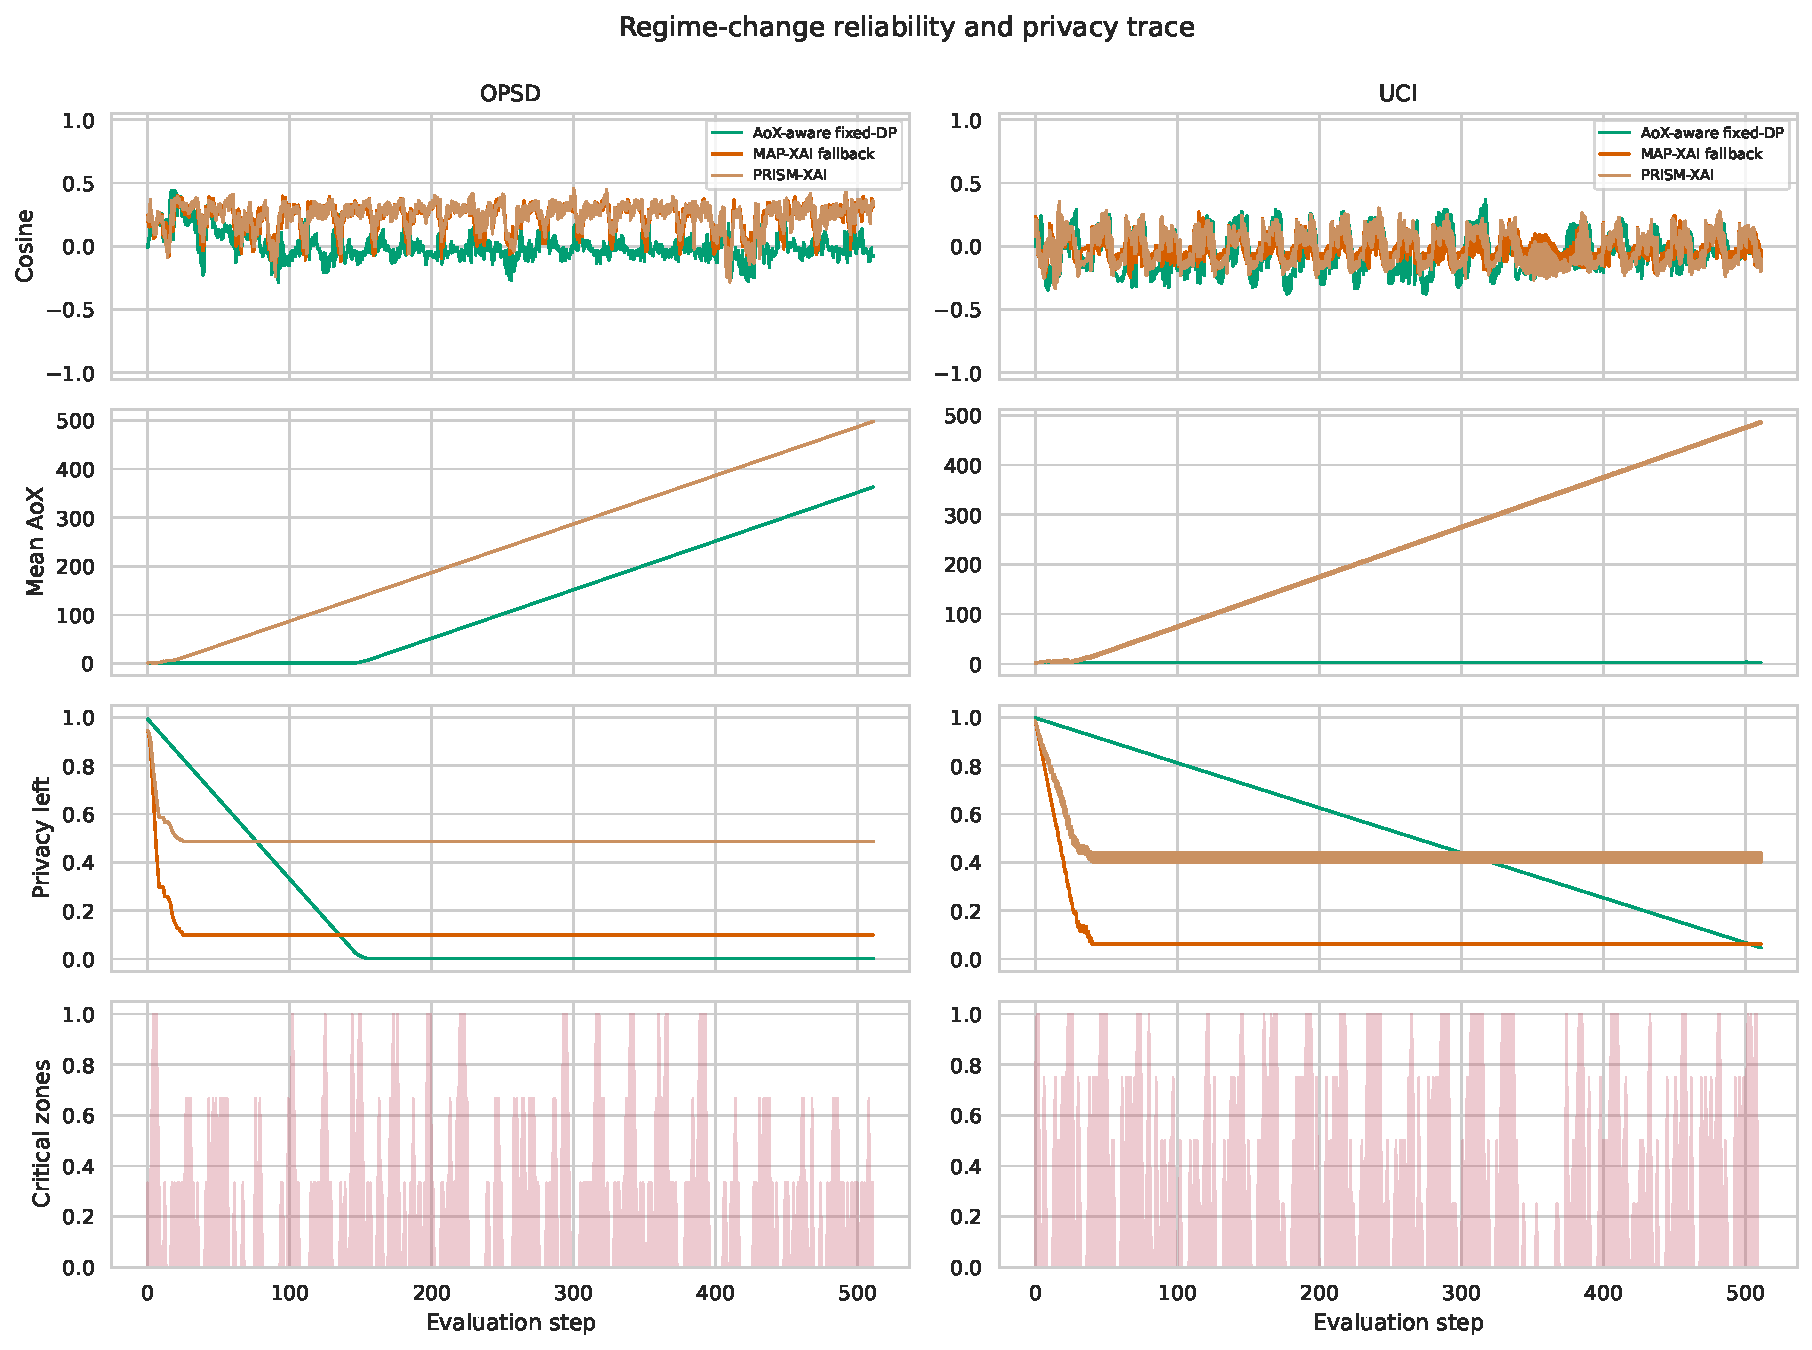
\includegraphics[width=.96\textwidth,height=.82\textheight,keepaspectratio]{../../SERVICE_TRADEOFF_RESULTS/runs/thr_1_cap_16/regime_trace.pdf}

\caption{Public-score threshold $\tau=1$, release cap $M=16$, Combined datasets: representative regime trace. This panel should be read with the setting-level quantitative interpretation and the complete tables immediately preceding the figure block.}

\end{figure*}

\clearpage

\begin{figure*}[p]

\centering

\includegraphics[width=.96\textwidth,height=.82\textheight,keepaspectratio]{../../SERVICE_TRADEOFF_RESULTS/runs/thr_1_cap_16/fairness_reliability.pdf}

\caption{Public-score threshold $\tau=1$, release cap $M=16$, Combined datasets: fairness--reliability plane. This panel should be read with the setting-level quantitative interpretation and the complete tables immediately preceding the figure block.}

\end{figure*}

\clearpage

\begin{figure*}[p]

\centering

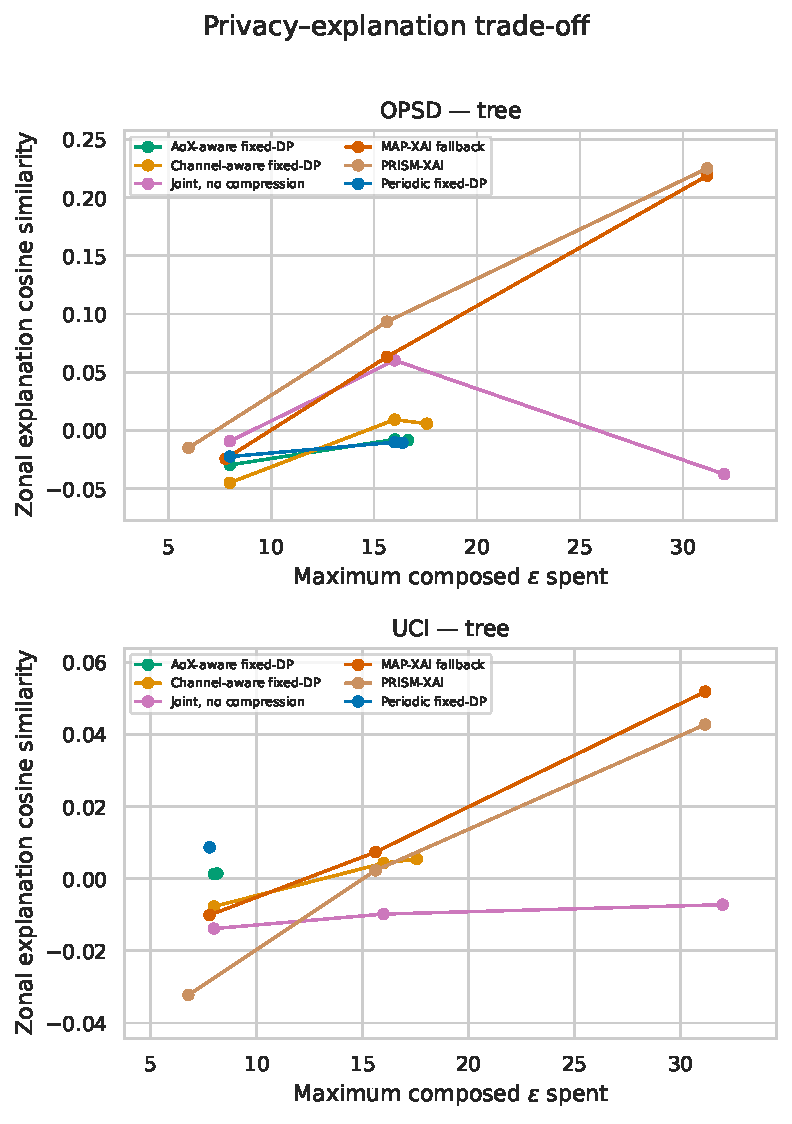
\includegraphics[width=.96\textwidth,height=.82\textheight,keepaspectratio]{../../SERVICE_TRADEOFF_RESULTS/runs/thr_1_cap_16/privacy_fidelity.pdf}

\caption{Public-score threshold $\tau=1$, release cap $M=16$, Combined datasets: privacy--fidelity plane. This panel should be read with the setting-level quantitative interpretation and the complete tables immediately preceding the figure block.}

\end{figure*}

\clearpage

\begin{figure*}[p]

\centering

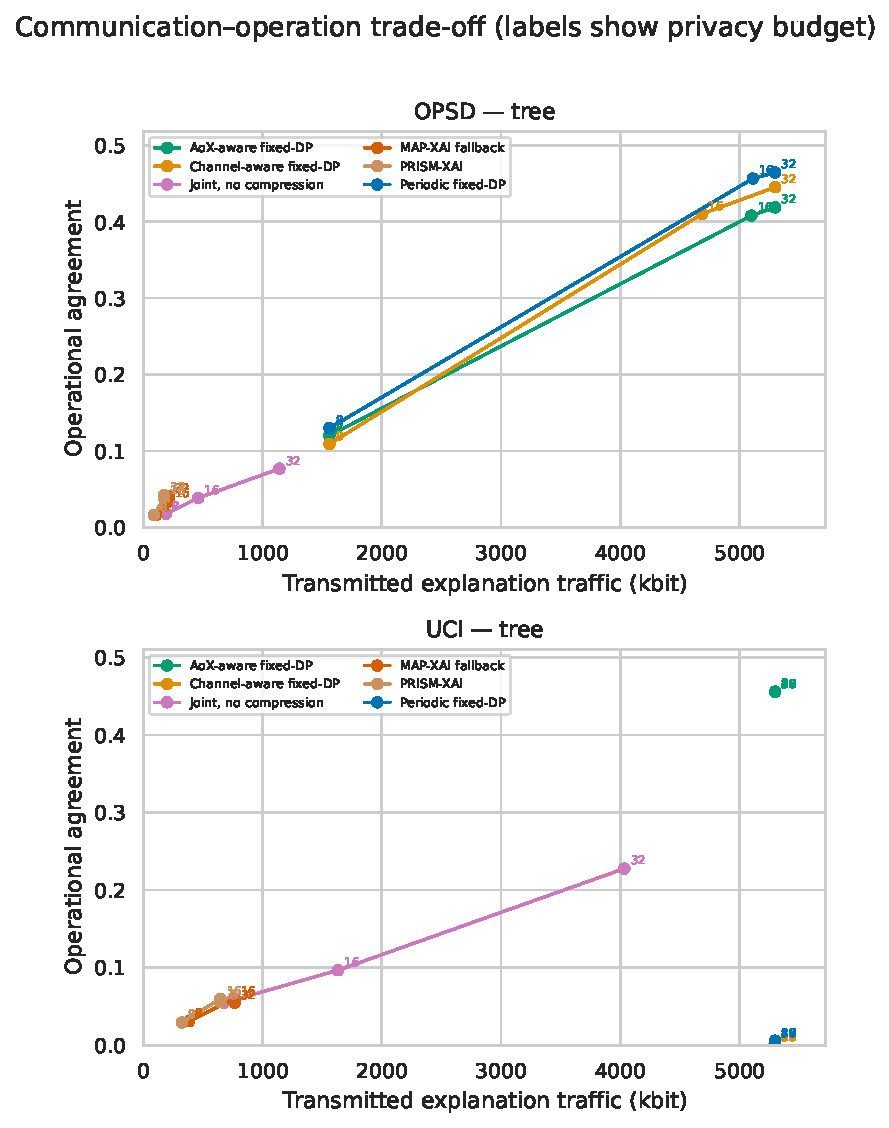
\includegraphics[width=.96\textwidth,height=.82\textheight,keepaspectratio]{../../SERVICE_TRADEOFF_RESULTS/runs/thr_1_cap_16/pareto_bits_fidelity.pdf}

\caption{Public-score threshold $\tau=1$, release cap $M=16$, Combined datasets: traffic--fidelity Pareto plane. This panel should be read with the setting-level quantitative interpretation and the complete tables immediately preceding the figure block.}

\end{figure*}

\clearpage

\begin{figure*}[p]

\centering

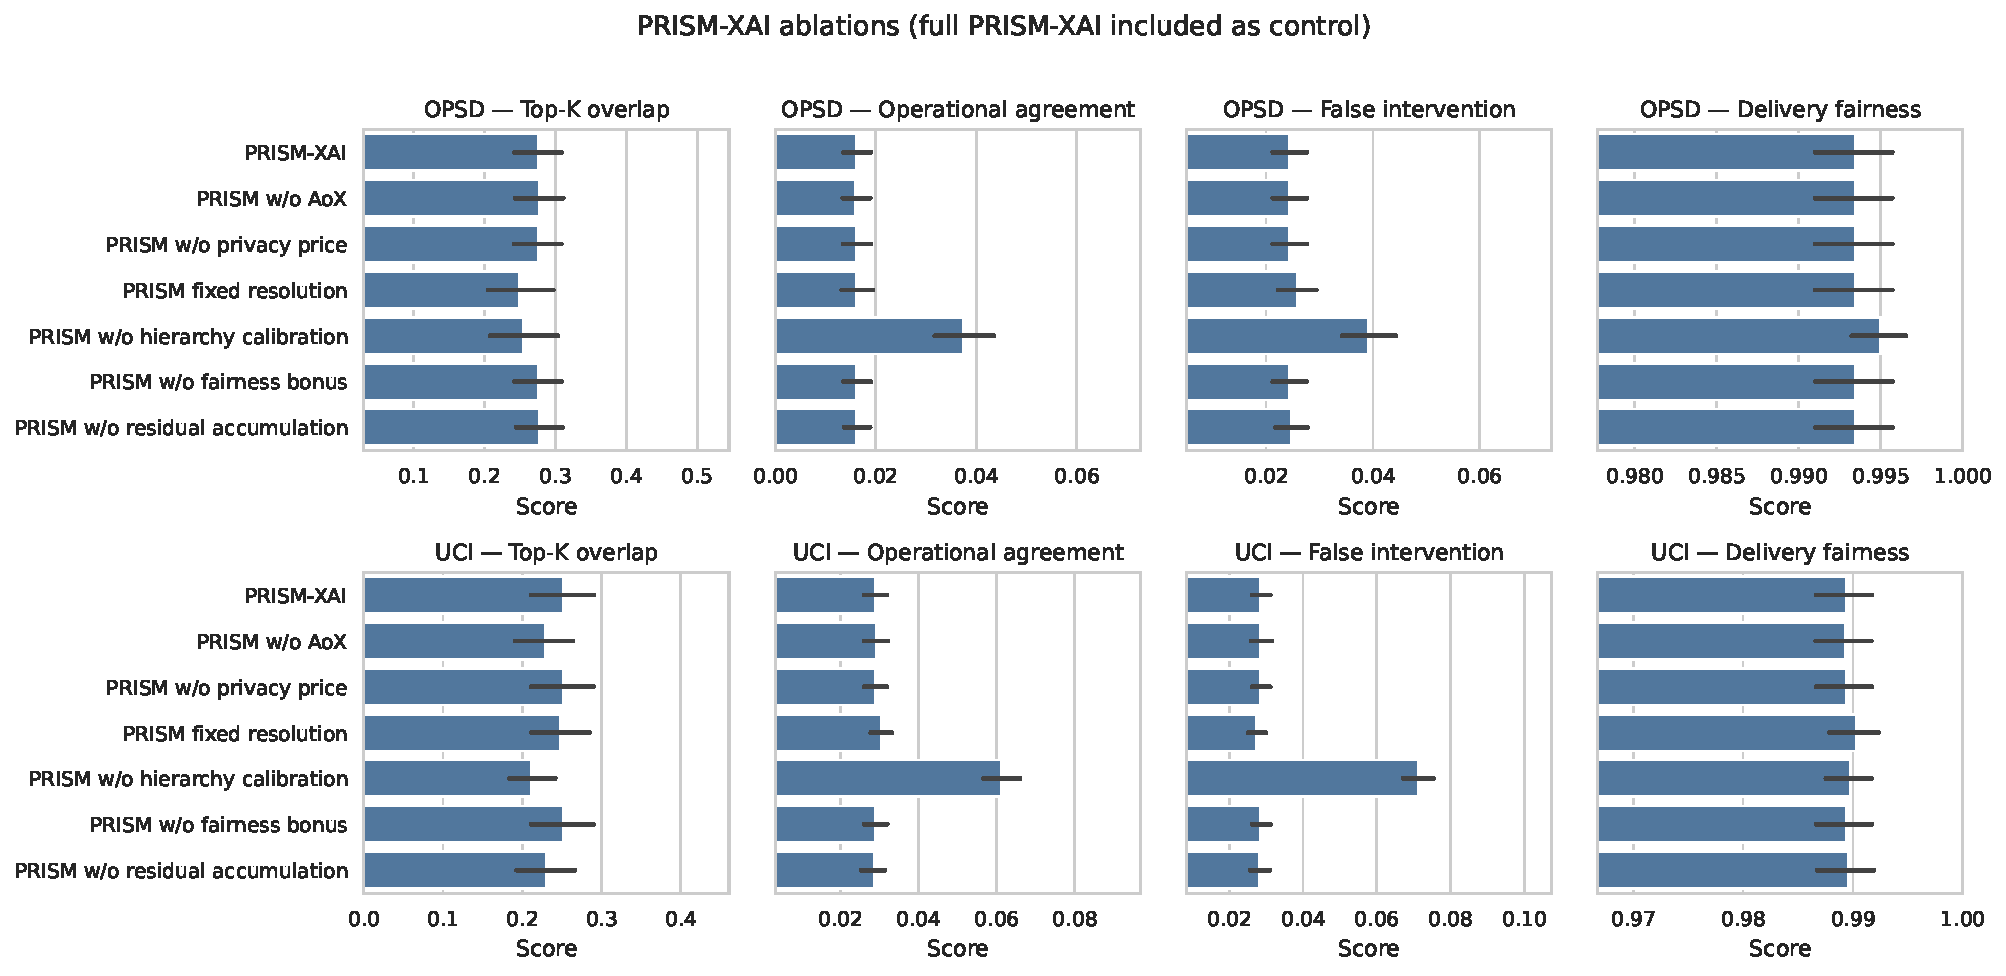
\includegraphics[width=.96\textwidth,height=.82\textheight,keepaspectratio]{../../SERVICE_TRADEOFF_RESULTS/runs/thr_1_cap_16/ablation_results.pdf}

\caption{Public-score threshold $\tau=1$, release cap $M=16$, Combined datasets: component ablation. This panel should be read with the setting-level quantitative interpretation and the complete tables immediately preceding the figure block.}

\end{figure*}

\clearpage

\paragraph{OPSD.} The three generated tables below report the full method means, all condition-level values, and paired differences. The five figures that follow provide the corresponding temporal, fairness, privacy, Pareto, and ablation views. Aggregate panels support the setting-level summary above; dataset panels reveal whether that summary is shared by OPSD and UCI rather than being driven by their different endpoint counts.

\begin{table*}[p]\centering\tiny

\caption{Public-score threshold $\tau=1$, release cap $M=16$, OPSD: complete generated method table.}

\label{tab:thr_1_cap_16:opsd:main}

\resizebox{\linewidth}{!}{% Values are means with 95% Student-t confidence intervals across seeds.
\begin{tabular}{lccccccccccccccc}
\toprule
Dataset & Model & $\epsilon_{\max}$ & Method & Top-$K$ & Cosine & Decision & Recall & Prec. & Abst. & P95 ms & kbit & Spent $\epsilon$ & False int. & bit/correct & Fairness \\
\midrule
OPSD & Tree & 8 & AoX-aware fixed-DP & 0.234 $\pm$ 0.048 & -0.033 $\pm$ 0.028 & 0.119 $\pm$ 0.028 & 0.119 $\pm$ 0.028 & 0.198 $\pm$ 0.054 & 0.721 $\pm$ 0.005 & 6.903 $\pm$ 1.126 & 1560.564 $\pm$ 0.000 & 7.990 $\pm$ 0.000 & 0.183 $\pm$ 0.020 & 35567.482 $\pm$ 10569.818 & 0.999 $\pm$ 0.000 \\
OPSD & Tree & 8 & AoX-aware fixed-DP & 0.238 $\pm$ 0.049 & -0.026 $\pm$ 0.055 & 0.121 $\pm$ 0.026 & 0.121 $\pm$ 0.026 & 0.205 $\pm$ 0.053 & 0.721 $\pm$ 0.005 & 6.903 $\pm$ 1.126 & 1560.564 $\pm$ 0.000 & 7.990 $\pm$ 0.000 & 0.179 $\pm$ 0.023 & 34123.214 $\pm$ 8376.542 & 0.999 $\pm$ 0.000 \\
OPSD & Tree & 8 & Channel-aware fixed-DP & 0.292 $\pm$ 0.037 & -0.041 $\pm$ 0.051 & 0.107 $\pm$ 0.026 & 0.107 $\pm$ 0.026 & 0.217 $\pm$ 0.068 & 0.779 $\pm$ 0.011 & 5.571 $\pm$ 1.784 & 1560.564 $\pm$ 0.000 & 7.990 $\pm$ 0.000 & 0.154 $\pm$ 0.029 & 40860.756 $\pm$ 14126.920 & 0.999 $\pm$ 0.000 \\
OPSD & Tree & 8 & Channel-aware fixed-DP & 0.292 $\pm$ 0.054 & -0.049 $\pm$ 0.064 & 0.111 $\pm$ 0.023 & 0.111 $\pm$ 0.023 & 0.228 $\pm$ 0.066 & 0.779 $\pm$ 0.011 & 5.571 $\pm$ 1.784 & 1560.564 $\pm$ 0.000 & 7.990 $\pm$ 0.000 & 0.149 $\pm$ 0.026 & 37980.855 $\pm$ 12338.094 & 0.999 $\pm$ 0.000 \\
OPSD & Tree & 8 & Joint, no compression & 0.288 $\pm$ 0.064 & -0.030 $\pm$ 0.079 & 0.016 $\pm$ 0.005 & 0.016 $\pm$ 0.005 & 0.193 $\pm$ 0.059 & 0.957 $\pm$ 0.003 & 4.560 $\pm$ 1.811 & 189.900 $\pm$ 0.554 & 7.990 $\pm$ 0.000 & 0.027 $\pm$ 0.005 & 32490.357 $\pm$ 10149.755 & 0.996 $\pm$ 0.002 \\
OPSD & Tree & 8 & Joint, no compression & 0.258 $\pm$ 0.055 & 0.011 $\pm$ 0.094 & 0.019 $\pm$ 0.004 & 0.019 $\pm$ 0.004 & 0.224 $\pm$ 0.044 & 0.957 $\pm$ 0.003 & 4.562 $\pm$ 1.809 & 189.750 $\pm$ 0.566 & 7.990 $\pm$ 0.000 & 0.025 $\pm$ 0.003 & 26079.167 $\pm$ 6335.386 & 0.996 $\pm$ 0.002 \\
OPSD & Tree & 8 & Periodic fixed-DP & 0.241 $\pm$ 0.049 & -0.019 $\pm$ 0.061 & 0.125 $\pm$ 0.020 & 0.125 $\pm$ 0.020 & 0.209 $\pm$ 0.044 & 0.722 $\pm$ 0.006 & 6.303 $\pm$ 1.438 & 1560.564 $\pm$ 0.000 & 7.990 $\pm$ 0.000 & 0.181 $\pm$ 0.021 & 31183.082 $\pm$ 4356.378 & 0.999 $\pm$ 0.000 \\
OPSD & Tree & 8 & Periodic fixed-DP & 0.242 $\pm$ 0.048 & -0.026 $\pm$ 0.082 & 0.135 $\pm$ 0.016 & 0.135 $\pm$ 0.016 & 0.231 $\pm$ 0.037 & 0.722 $\pm$ 0.006 & 6.303 $\pm$ 1.438 & 1560.564 $\pm$ 0.000 & 7.990 $\pm$ 0.000 & 0.169 $\pm$ 0.017 & 28520.235 $\pm$ 3511.595 & 0.999 $\pm$ 0.000 \\
OPSD & Tree & 8 & PRISM-XAI & 0.270 $\pm$ 0.066 & -0.025 $\pm$ 0.093 & 0.015 $\pm$ 0.004 & 0.015 $\pm$ 0.004 & 0.200 $\pm$ 0.078 & 0.956 $\pm$ 0.003 & 4.630 $\pm$ 1.839 & 87.697 $\pm$ 0.410 & 6.034 $\pm$ 0.230 & 0.025 $\pm$ 0.005 & 15451.736 $\pm$ 3728.991 & 0.993 $\pm$ 0.004 \\
OPSD & Tree & 8 & PRISM-XAI & 0.283 $\pm$ 0.054 & -0.005 $\pm$ 0.086 & 0.017 $\pm$ 0.005 & 0.017 $\pm$ 0.005 & 0.222 $\pm$ 0.080 & 0.956 $\pm$ 0.003 & 4.630 $\pm$ 1.839 & 87.431 $\pm$ 0.364 & 5.936 $\pm$ 0.213 & 0.024 $\pm$ 0.005 & 14279.307 $\pm$ 3768.065 & 0.993 $\pm$ 0.004 \\
OPSD & Tree & 8 & MAP-XAI fallback & 0.234 $\pm$ 0.073 & -0.037 $\pm$ 0.075 & 0.016 $\pm$ 0.005 & 0.016 $\pm$ 0.005 & 0.191 $\pm$ 0.080 & 0.956 $\pm$ 0.003 & 4.732 $\pm$ 1.776 & 105.817 $\pm$ 0.049 & 7.786 $\pm$ 0.000 & 0.027 $\pm$ 0.006 & 21385.963 $\pm$ 9729.377 & 0.993 $\pm$ 0.004 \\
OPSD & Tree & 8 & MAP-XAI fallback & 0.230 $\pm$ 0.067 & -0.012 $\pm$ 0.085 & 0.017 $\pm$ 0.005 & 0.017 $\pm$ 0.005 & 0.219 $\pm$ 0.073 & 0.956 $\pm$ 0.003 & 4.732 $\pm$ 1.776 & 105.675 $\pm$ 0.049 & 7.786 $\pm$ 0.000 & 0.024 $\pm$ 0.006 & 19083.433 $\pm$ 9057.454 & 0.993 $\pm$ 0.004 \\
\bottomrule
\end{tabular}
}

\end{table*}\clearpage

\begin{table*}[p]\centering\tiny

\caption{Public-score threshold $\tau=1$, release cap $M=16$, OPSD: complete condition-level generated table.}

\label{tab:thr_1_cap_16:opsd:conditions}

\resizebox{\textwidth}{!}{\begin{tabular}{llllccccccccccc}
\toprule
Dataset & Model & $\epsilon_{\max}$ & Method & kbit & Top-$K$ & Random Top-$K$ & Cosine & Decision & Recall & Precision & Coverage & Abstain & False int. & Spent $\epsilon$ \\
\midrule
OPSD & Tree & 8 & Joint, no compression & 189.900 $\pm$ 0.554 & 0.288 $\pm$ 0.064 & 0.250 $\pm$ 0.000 & -0.030 $\pm$ 0.079 & 0.016 $\pm$ 0.005 & 0.016 $\pm$ 0.005 & 0.193 $\pm$ 0.059 & 0.043 $\pm$ 0.003 & 0.957 $\pm$ 0.003 & 0.027 $\pm$ 0.005 & 7.990 $\pm$ 0.000 \\
OPSD & Tree & 8 & Joint, no compression & 189.750 $\pm$ 0.566 & 0.258 $\pm$ 0.055 & 0.250 $\pm$ 0.000 & 0.011 $\pm$ 0.094 & 0.019 $\pm$ 0.004 & 0.019 $\pm$ 0.004 & 0.224 $\pm$ 0.044 & 0.043 $\pm$ 0.003 & 0.957 $\pm$ 0.003 & 0.025 $\pm$ 0.003 & 7.990 $\pm$ 0.000 \\
OPSD & Tree & 8 & Periodic fixed-DP & 1560.564 $\pm$ 0.000 & 0.241 $\pm$ 0.049 & 0.250 $\pm$ 0.000 & -0.019 $\pm$ 0.061 & 0.125 $\pm$ 0.020 & 0.125 $\pm$ 0.020 & 0.209 $\pm$ 0.044 & 0.278 $\pm$ 0.006 & 0.722 $\pm$ 0.006 & 0.181 $\pm$ 0.021 & 7.990 $\pm$ 0.000 \\
OPSD & Tree & 8 & Periodic fixed-DP & 1560.564 $\pm$ 0.000 & 0.242 $\pm$ 0.048 & 0.250 $\pm$ 0.000 & -0.026 $\pm$ 0.082 & 0.135 $\pm$ 0.016 & 0.135 $\pm$ 0.016 & 0.231 $\pm$ 0.037 & 0.278 $\pm$ 0.006 & 0.722 $\pm$ 0.006 & 0.169 $\pm$ 0.017 & 7.990 $\pm$ 0.000 \\
OPSD & Tree & 8 & PRISM-XAI & 87.697 $\pm$ 0.410 & 0.270 $\pm$ 0.066 & 0.250 $\pm$ 0.000 & -0.025 $\pm$ 0.093 & 0.015 $\pm$ 0.004 & 0.015 $\pm$ 0.004 & 0.200 $\pm$ 0.078 & 0.044 $\pm$ 0.003 & 0.956 $\pm$ 0.003 & 0.025 $\pm$ 0.005 & 6.034 $\pm$ 0.230 \\
OPSD & Tree & 8 & PRISM-XAI & 87.431 $\pm$ 0.364 & 0.283 $\pm$ 0.054 & 0.250 $\pm$ 0.000 & -0.005 $\pm$ 0.086 & 0.017 $\pm$ 0.005 & 0.017 $\pm$ 0.005 & 0.222 $\pm$ 0.080 & 0.044 $\pm$ 0.003 & 0.956 $\pm$ 0.003 & 0.024 $\pm$ 0.005 & 5.936 $\pm$ 0.213 \\
OPSD & Tree & 16 & Joint, no compression & 459.900 $\pm$ 0.750 & 0.232 $\pm$ 0.065 & 0.250 $\pm$ 0.000 & 0.059 $\pm$ 0.048 & 0.038 $\pm$ 0.009 & 0.038 $\pm$ 0.009 & 0.222 $\pm$ 0.049 & 0.088 $\pm$ 0.004 & 0.912 $\pm$ 0.004 & 0.049 $\pm$ 0.005 & 15.997 $\pm$ 0.000 \\
OPSD & Tree & 16 & Joint, no compression & 460.050 $\pm$ 0.724 & 0.241 $\pm$ 0.055 & 0.250 $\pm$ 0.000 & 0.061 $\pm$ 0.052 & 0.039 $\pm$ 0.008 & 0.039 $\pm$ 0.008 & 0.241 $\pm$ 0.042 & 0.088 $\pm$ 0.004 & 0.912 $\pm$ 0.004 & 0.045 $\pm$ 0.004 & 15.997 $\pm$ 0.000 \\
OPSD & Tree & 16 & Periodic fixed-DP & 5112.594 $\pm$ 0.000 & 0.249 $\pm$ 0.022 & 0.250 $\pm$ 0.000 & -0.009 $\pm$ 0.045 & 0.450 $\pm$ 0.062 & 0.450 $\pm$ 0.062 & 0.237 $\pm$ 0.042 & 0.985 $\pm$ 0.002 & 0.015 $\pm$ 0.002 & 0.551 $\pm$ 0.057 & 15.997 $\pm$ 0.000 \\
OPSD & Tree & 16 & Periodic fixed-DP & 5112.594 $\pm$ 0.000 & 0.243 $\pm$ 0.019 & 0.250 $\pm$ 0.000 & -0.012 $\pm$ 0.050 & 0.463 $\pm$ 0.047 & 0.463 $\pm$ 0.047 & 0.240 $\pm$ 0.028 & 0.985 $\pm$ 0.002 & 0.015 $\pm$ 0.002 & 0.547 $\pm$ 0.036 & 15.997 $\pm$ 0.000 \\
OPSD & Tree & 16 & PRISM-XAI & 175.005 $\pm$ 0.564 & 0.242 $\pm$ 0.064 & 0.250 $\pm$ 0.000 & 0.085 $\pm$ 0.083 & 0.039 $\pm$ 0.008 & 0.039 $\pm$ 0.008 & 0.287 $\pm$ 0.077 & 0.081 $\pm$ 0.003 & 0.919 $\pm$ 0.003 & 0.038 $\pm$ 0.008 & 15.620 $\pm$ 0.000 \\
OPSD & Tree & 16 & PRISM-XAI & 174.493 $\pm$ 0.509 & 0.213 $\pm$ 0.052 & 0.250 $\pm$ 0.000 & 0.102 $\pm$ 0.085 & 0.037 $\pm$ 0.009 & 0.037 $\pm$ 0.009 & 0.264 $\pm$ 0.059 & 0.081 $\pm$ 0.003 & 0.919 $\pm$ 0.003 & 0.039 $\pm$ 0.007 & 15.620 $\pm$ 0.000 \\
OPSD & Tree & 32 & Joint, no compression & 1140.900 $\pm$ 7.953 & 0.235 $\pm$ 0.064 & 0.250 $\pm$ 0.000 & -0.031 $\pm$ 0.089 & 0.074 $\pm$ 0.015 & 0.074 $\pm$ 0.015 & 0.205 $\pm$ 0.039 & 0.157 $\pm$ 0.006 & 0.843 $\pm$ 0.006 & 0.107 $\pm$ 0.009 & 31.999 $\pm$ 0.000 \\
OPSD & Tree & 32 & Joint, no compression & 1140.900 $\pm$ 7.953 & 0.282 $\pm$ 0.054 & 0.250 $\pm$ 0.000 & -0.044 $\pm$ 0.076 & 0.080 $\pm$ 0.011 & 0.080 $\pm$ 0.011 & 0.227 $\pm$ 0.052 & 0.158 $\pm$ 0.006 & 0.842 $\pm$ 0.006 & 0.105 $\pm$ 0.015 & 31.999 $\pm$ 0.000 \\
OPSD & Tree & 32 & Periodic fixed-DP & 5299.836 $\pm$ 0.625 & 0.249 $\pm$ 0.022 & 0.250 $\pm$ 0.000 & -0.009 $\pm$ 0.044 & 0.458 $\pm$ 0.066 & 0.458 $\pm$ 0.066 & 0.237 $\pm$ 0.045 & 1.000 $\pm$ 0.000 & 0.000 $\pm$ 0.000 & 0.562 $\pm$ 0.062 & 16.371 $\pm$ 0.000 \\
OPSD & Tree & 32 & Periodic fixed-DP & 5299.836 $\pm$ 0.625 & 0.244 $\pm$ 0.019 & 0.250 $\pm$ 0.000 & -0.012 $\pm$ 0.050 & 0.471 $\pm$ 0.049 & 0.471 $\pm$ 0.049 & 0.240 $\pm$ 0.029 & 1.000 $\pm$ 0.000 & 0.000 $\pm$ 0.000 & 0.559 $\pm$ 0.039 & 16.371 $\pm$ 0.000 \\
OPSD & Tree & 32 & PRISM-XAI & 174.944 $\pm$ 0.552 & 0.309 $\pm$ 0.062 & 0.250 $\pm$ 0.000 & 0.203 $\pm$ 0.080 & 0.043 $\pm$ 0.009 & 0.043 $\pm$ 0.009 & 0.336 $\pm$ 0.099 & 0.081 $\pm$ 0.003 & 0.919 $\pm$ 0.003 & 0.033 $\pm$ 0.008 & 31.175 $\pm$ 0.000 \\
OPSD & Tree & 32 & PRISM-XAI & 174.309 $\pm$ 0.461 & 0.326 $\pm$ 0.085 & 0.250 $\pm$ 0.000 & 0.247 $\pm$ 0.077 & 0.042 $\pm$ 0.009 & 0.042 $\pm$ 0.009 & 0.294 $\pm$ 0.073 & 0.081 $\pm$ 0.003 & 0.919 $\pm$ 0.003 & 0.039 $\pm$ 0.007 & 31.175 $\pm$ 0.000 \\
\bottomrule
\end{tabular}
}

\end{table*}\clearpage

\begin{table*}[p]\centering\tiny

\caption{Public-score threshold $\tau=1$, release cap $M=16$, OPSD: complete generated paired comparisons.}

\label{tab:thr_1_cap_16:opsd:paired}

\resizebox{\textwidth}{!}{\begin{tabular}{llcccc}
\toprule
Dataset & Baseline & Delta kbit & Delta Top-$K$ & Delta recall & Delta fairness \\
\midrule
OPSD & AoX-aware fixed-DP & -1472.867 $\pm$ 0.410 & 0.036 $\pm$ 0.086 & -0.104 $\pm$ 0.029 & -0.006 $\pm$ 0.004 \\
OPSD & AoX-aware fixed-DP & -4924.908 $\pm$ 5.576 & -0.011 $\pm$ 0.052 & -0.362 $\pm$ 0.075 & -0.004 $\pm$ 0.002 \\
OPSD & AoX-aware fixed-DP & -5125.280 $\pm$ 0.552 & 0.056 $\pm$ 0.077 & -0.370 $\pm$ 0.075 & -0.003 $\pm$ 0.002 \\
OPSD & AoX-aware fixed-DP & -1473.133 $\pm$ 0.364 & 0.045 $\pm$ 0.066 & -0.104 $\pm$ 0.027 & -0.006 $\pm$ 0.004 \\
OPSD & AoX-aware fixed-DP & -4925.420 $\pm$ 5.602 & -0.039 $\pm$ 0.045 & -0.378 $\pm$ 0.056 & -0.004 $\pm$ 0.002 \\
OPSD & AoX-aware fixed-DP & -5125.915 $\pm$ 0.461 & 0.074 $\pm$ 0.085 & -0.384 $\pm$ 0.056 & -0.004 $\pm$ 0.002 \\
OPSD & Channel-aware fixed-DP & -1472.867 $\pm$ 0.410 & -0.023 $\pm$ 0.091 & -0.092 $\pm$ 0.025 & -0.006 $\pm$ 0.004 \\
OPSD & Channel-aware fixed-DP & -4511.604 $\pm$ 12.966 & -0.019 $\pm$ 0.055 & -0.362 $\pm$ 0.090 & 0.058 $\pm$ 0.005 \\
OPSD & Channel-aware fixed-DP & -5125.280 $\pm$ 0.552 & 0.051 $\pm$ 0.072 & -0.392 $\pm$ 0.096 & 0.089 $\pm$ 0.006 \\
OPSD & Channel-aware fixed-DP & -1473.133 $\pm$ 0.364 & -0.010 $\pm$ 0.076 & -0.094 $\pm$ 0.024 & -0.006 $\pm$ 0.004 \\
OPSD & Channel-aware fixed-DP & -4512.116 $\pm$ 12.805 & -0.045 $\pm$ 0.039 & -0.382 $\pm$ 0.087 & 0.058 $\pm$ 0.005 \\
OPSD & Channel-aware fixed-DP & -5125.915 $\pm$ 0.461 & 0.069 $\pm$ 0.081 & -0.414 $\pm$ 0.089 & 0.089 $\pm$ 0.006 \\
OPSD & Joint, no compression & -102.203 $\pm$ 0.525 & -0.018 $\pm$ 0.097 & -0.001 $\pm$ 0.004 & -0.002 $\pm$ 0.003 \\
OPSD & Joint, no compression & -284.895 $\pm$ 1.260 & 0.011 $\pm$ 0.071 & 0.001 $\pm$ 0.011 & -0.001 $\pm$ 0.002 \\
OPSD & Joint, no compression & -965.956 $\pm$ 8.155 & 0.073 $\pm$ 0.062 & -0.031 $\pm$ 0.015 & -0.003 $\pm$ 0.002 \\
OPSD & Joint, no compression & -102.319 $\pm$ 0.436 & 0.024 $\pm$ 0.089 & -0.002 $\pm$ 0.003 & -0.002 $\pm$ 0.003 \\
OPSD & Joint, no compression & -285.557 $\pm$ 1.134 & -0.027 $\pm$ 0.062 & -0.002 $\pm$ 0.012 & -0.001 $\pm$ 0.002 \\
OPSD & Joint, no compression & -966.591 $\pm$ 8.036 & 0.044 $\pm$ 0.085 & -0.038 $\pm$ 0.011 & -0.003 $\pm$ 0.002 \\
OPSD & Periodic fixed-DP & -1472.867 $\pm$ 0.410 & 0.029 $\pm$ 0.092 & -0.110 $\pm$ 0.020 & -0.006 $\pm$ 0.004 \\
OPSD & Periodic fixed-DP & -4937.589 $\pm$ 0.564 & -0.007 $\pm$ 0.060 & -0.411 $\pm$ 0.063 & -0.004 $\pm$ 0.002 \\
OPSD & Periodic fixed-DP & -5124.892 $\pm$ 0.754 & 0.060 $\pm$ 0.073 & -0.415 $\pm$ 0.064 & -0.004 $\pm$ 0.002 \\
OPSD & Periodic fixed-DP & -1473.133 $\pm$ 0.364 & 0.041 $\pm$ 0.073 & -0.118 $\pm$ 0.016 & -0.006 $\pm$ 0.004 \\
OPSD & Periodic fixed-DP & -4938.101 $\pm$ 0.509 & -0.029 $\pm$ 0.052 & -0.426 $\pm$ 0.048 & -0.004 $\pm$ 0.002 \\
OPSD & Periodic fixed-DP & -5125.527 $\pm$ 0.718 & 0.082 $\pm$ 0.090 & -0.429 $\pm$ 0.048 & -0.004 $\pm$ 0.002 \\
OPSD & MAP-XAI fallback & -18.120 $\pm$ 0.422 & 0.035 $\pm$ 0.088 & -0.000 $\pm$ 0.003 & 0.000 $\pm$ 0.000 \\
OPSD & MAP-XAI fallback & -38.812 $\pm$ 0.567 & -0.011 $\pm$ 0.064 & 0.004 $\pm$ 0.008 & 0.000 $\pm$ 0.000 \\
OPSD & MAP-XAI fallback & -38.873 $\pm$ 0.554 & -0.004 $\pm$ 0.061 & 0.003 $\pm$ 0.006 & 0.000 $\pm$ 0.000 \\
OPSD & MAP-XAI fallback & -18.245 $\pm$ 0.372 & 0.053 $\pm$ 0.042 & -0.000 $\pm$ 0.004 & 0.000 $\pm$ 0.000 \\
OPSD & MAP-XAI fallback & -39.182 $\pm$ 0.498 & -0.034 $\pm$ 0.034 & 0.004 $\pm$ 0.009 & 0.000 $\pm$ 0.000 \\
OPSD & MAP-XAI fallback & -39.346 $\pm$ 0.444 & 0.055 $\pm$ 0.050 & 0.001 $\pm$ 0.005 & -0.000 $\pm$ 0.001 \\
\bottomrule
\end{tabular}
}

\end{table*}\clearpage

\begin{figure*}[p]

\centering

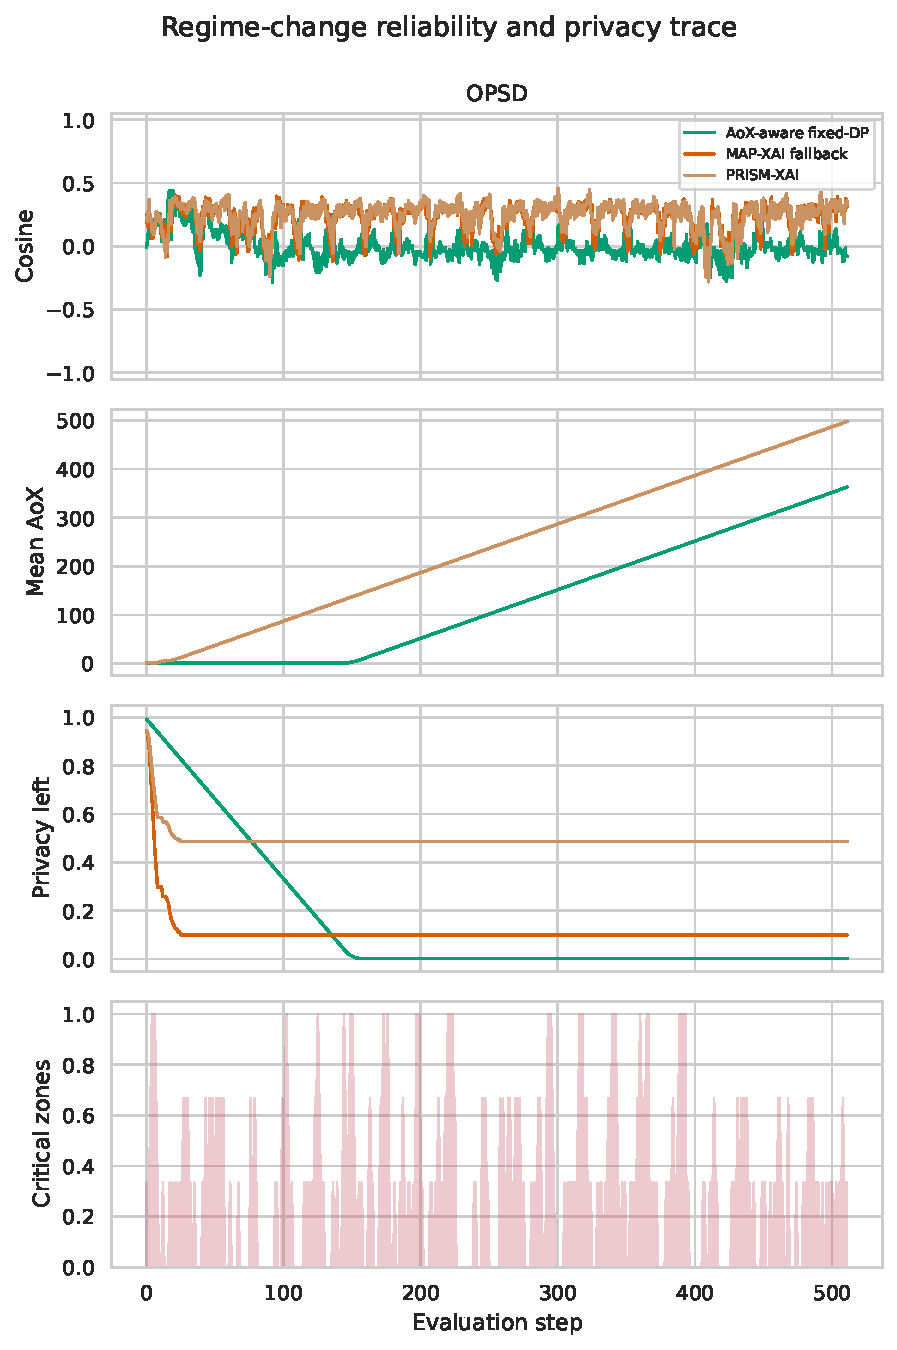
\includegraphics[width=.96\textwidth,height=.82\textheight,keepaspectratio]{../../SERVICE_TRADEOFF_RESULTS/runs/thr_1_cap_16/opsd/regime_trace.pdf}

\caption{Public-score threshold $\tau=1$, release cap $M=16$, OPSD: representative regime trace. This panel should be read with the setting-level quantitative interpretation and the complete tables immediately preceding the figure block.}

\end{figure*}

\clearpage

\begin{figure*}[p]

\centering

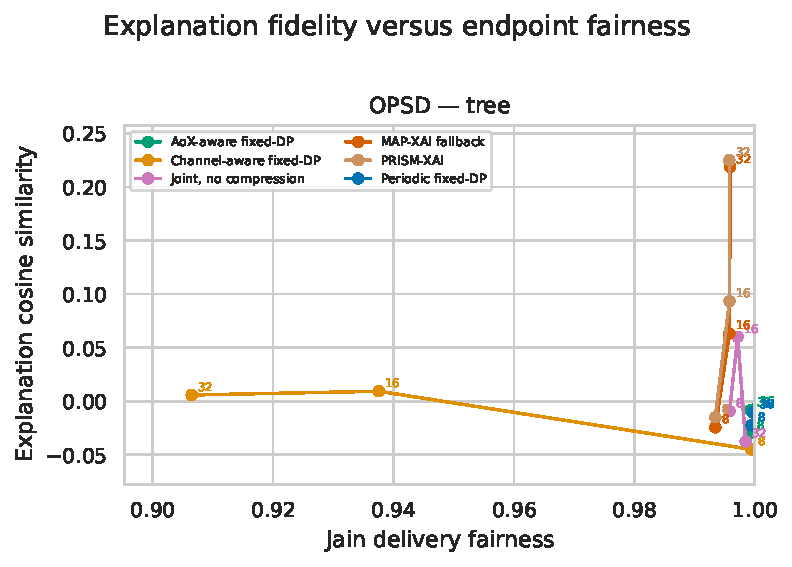
\includegraphics[width=.96\textwidth,height=.82\textheight,keepaspectratio]{../../SERVICE_TRADEOFF_RESULTS/runs/thr_1_cap_16/opsd/fairness_reliability.pdf}

\caption{Public-score threshold $\tau=1$, release cap $M=16$, OPSD: fairness--reliability plane. This panel should be read with the setting-level quantitative interpretation and the complete tables immediately preceding the figure block.}

\end{figure*}

\clearpage

\begin{figure*}[p]

\centering

\includegraphics[width=.96\textwidth,height=.82\textheight,keepaspectratio]{../../SERVICE_TRADEOFF_RESULTS/runs/thr_1_cap_16/opsd/privacy_fidelity.pdf}

\caption{Public-score threshold $\tau=1$, release cap $M=16$, OPSD: privacy--fidelity plane. This panel should be read with the setting-level quantitative interpretation and the complete tables immediately preceding the figure block.}

\end{figure*}

\clearpage

\begin{figure*}[p]

\centering

\includegraphics[width=.96\textwidth,height=.82\textheight,keepaspectratio]{../../SERVICE_TRADEOFF_RESULTS/runs/thr_1_cap_16/opsd/pareto_bits_fidelity.pdf}

\caption{Public-score threshold $\tau=1$, release cap $M=16$, OPSD: traffic--fidelity Pareto plane. This panel should be read with the setting-level quantitative interpretation and the complete tables immediately preceding the figure block.}

\end{figure*}

\clearpage

\begin{figure*}[p]

\centering

\includegraphics[width=.96\textwidth,height=.82\textheight,keepaspectratio]{../../SERVICE_TRADEOFF_RESULTS/runs/thr_1_cap_16/opsd/ablation_results.pdf}

\caption{Public-score threshold $\tau=1$, release cap $M=16$, OPSD: component ablation. This panel should be read with the setting-level quantitative interpretation and the complete tables immediately preceding the figure block.}

\end{figure*}

\clearpage

\paragraph{UCI.} The three generated tables below report the full method means, all condition-level values, and paired differences. The five figures that follow provide the corresponding temporal, fairness, privacy, Pareto, and ablation views. Aggregate panels support the setting-level summary above; dataset panels reveal whether that summary is shared by OPSD and UCI rather than being driven by their different endpoint counts.

\begin{table*}[p]\centering\tiny

\caption{Public-score threshold $\tau=1$, release cap $M=16$, UCI: complete generated method table.}

\label{tab:thr_1_cap_16:uci:main}

\resizebox{\linewidth}{!}{% Values are means with 95% Student-t confidence intervals across seeds.
\begin{tabular}{lccccccccccccccc}
\toprule
Dataset & Model & $\epsilon_{\max}$ & Method & Top-$K$ & Cosine & Decision & Recall & Prec. & Abst. & P95 ms & kbit & Spent $\epsilon$ & False int. & bit/correct & Fairness \\
\midrule
UCI & Tree & 8 & AoX-aware fixed-DP & 0.263 $\pm$ 0.041 & -0.007 $\pm$ 0.009 & 0.457 $\pm$ 0.031 & 0.457 $\pm$ 0.031 & 0.362 $\pm$ 0.024 & 0.003 $\pm$ 0.001 & 7.500 $\pm$ 0.000 & 5300.224 $\pm$ 0.000 & 7.990 $\pm$ 0.000 & 0.557 $\pm$ 0.025 & 14002.896 $\pm$ 1040.243 & 0.999 $\pm$ 0.000 \\
UCI & Tree & 8 & AoX-aware fixed-DP & 0.260 $\pm$ 0.022 & 0.010 $\pm$ 0.055 & 0.455 $\pm$ 0.047 & 0.455 $\pm$ 0.047 & 0.361 $\pm$ 0.038 & 0.003 $\pm$ 0.001 & 7.500 $\pm$ 0.000 & 5300.224 $\pm$ 0.000 & 7.990 $\pm$ 0.000 & 0.557 $\pm$ 0.048 & 14198.303 $\pm$ 1508.274 & 0.999 $\pm$ 0.000 \\
UCI & Tree & 8 & Channel-aware fixed-DP & 0.248 $\pm$ 0.031 & 0.004 $\pm$ 0.012 & 0.001 $\pm$ 0.001 & 0.001 $\pm$ 0.001 & 0.150 $\pm$ 0.151 & 0.999 $\pm$ 0.001 & 4.609 $\pm$ 1.781 & 5295.177 $\pm$ 3.740 & 7.990 $\pm$ 0.000 & 0.001 $\pm$ 0.001 & 4632196.500 $\pm$ 2102650.252 & 0.991 $\pm$ 0.001 \\
UCI & Tree & 8 & Channel-aware fixed-DP & 0.239 $\pm$ 0.030 & -0.020 $\pm$ 0.055 & 0.000 $\pm$ 0.000 & 0.000 $\pm$ 0.000 & 0.117 $\pm$ 0.225 & 0.999 $\pm$ 0.001 & 4.609 $\pm$ 1.781 & 5295.177 $\pm$ 3.740 & 7.990 $\pm$ 0.000 & 0.001 $\pm$ 0.001 & 5296989.000 $\pm$ 41104.572 & 0.991 $\pm$ 0.001 \\
UCI & Tree & 8 & Joint, no compression & 0.286 $\pm$ 0.045 & 0.004 $\pm$ 0.020 & 0.052 $\pm$ 0.005 & 0.052 $\pm$ 0.005 & 0.406 $\pm$ 0.037 & 0.875 $\pm$ 0.003 & 5.123 $\pm$ 1.792 & 672.300 $\pm$ 0.452 & 7.990 $\pm$ 0.000 & 0.053 $\pm$ 0.004 & 15676.175 $\pm$ 1475.621 & 0.994 $\pm$ 0.003 \\
UCI & Tree & 8 & Joint, no compression & 0.229 $\pm$ 0.052 & -0.032 $\pm$ 0.050 & 0.057 $\pm$ 0.007 & 0.057 $\pm$ 0.007 & 0.428 $\pm$ 0.041 & 0.875 $\pm$ 0.003 & 5.131 $\pm$ 1.787 & 672.300 $\pm$ 0.452 & 7.990 $\pm$ 0.000 & 0.052 $\pm$ 0.004 & 14702.786 $\pm$ 2334.488 & 0.994 $\pm$ 0.003 \\
UCI & Tree & 8 & Periodic fixed-DP & 0.259 $\pm$ 0.060 & -0.005 $\pm$ 0.008 & 0.006 $\pm$ 0.001 & 0.006 $\pm$ 0.001 & 0.244 $\pm$ 0.049 & 0.989 $\pm$ 0.001 & 4.596 $\pm$ 1.788 & 5299.318 $\pm$ 1.451 & 7.786 $\pm$ 0.000 & 0.013 $\pm$ 0.002 & 1215103.896 $\pm$ 390671.319 & 0.999 $\pm$ 0.000 \\
UCI & Tree & 8 & Periodic fixed-DP & 0.260 $\pm$ 0.044 & 0.022 $\pm$ 0.070 & 0.005 $\pm$ 0.001 & 0.005 $\pm$ 0.001 & 0.195 $\pm$ 0.050 & 0.989 $\pm$ 0.001 & 4.596 $\pm$ 1.788 & 5299.318 $\pm$ 1.451 & 7.786 $\pm$ 0.000 & 0.015 $\pm$ 0.002 & 1555837.203 $\pm$ 955472.503 & 0.999 $\pm$ 0.000 \\
UCI & Tree & 8 & PRISM-XAI & 0.240 $\pm$ 0.089 & -0.008 $\pm$ 0.019 & 0.031 $\pm$ 0.004 & 0.031 $\pm$ 0.004 & 0.422 $\pm$ 0.039 & 0.931 $\pm$ 0.004 & 6.267 $\pm$ 1.448 & 323.739 $\pm$ 1.239 & 6.844 $\pm$ 0.203 & 0.030 $\pm$ 0.005 & 13090.115 $\pm$ 2761.149 & 0.990 $\pm$ 0.003 \\
UCI & Tree & 8 & PRISM-XAI & 0.264 $\pm$ 0.044 & -0.056 $\pm$ 0.057 & 0.027 $\pm$ 0.005 & 0.027 $\pm$ 0.005 & 0.404 $\pm$ 0.063 & 0.938 $\pm$ 0.003 & 4.814 $\pm$ 1.710 & 321.228 $\pm$ 1.066 & 6.726 $\pm$ 0.146 & 0.027 $\pm$ 0.004 & 15136.774 $\pm$ 2629.908 & 0.989 $\pm$ 0.006 \\
UCI & Tree & 8 & MAP-XAI fallback & 0.240 $\pm$ 0.077 & -0.011 $\pm$ 0.019 & 0.032 $\pm$ 0.005 & 0.032 $\pm$ 0.005 & 0.446 $\pm$ 0.058 & 0.931 $\pm$ 0.004 & 5.672 $\pm$ 1.709 & 382.099 $\pm$ 0.159 & 7.786 $\pm$ 0.000 & 0.027 $\pm$ 0.003 & 15488.351 $\pm$ 4957.026 & 0.991 $\pm$ 0.003 \\
UCI & Tree & 8 & MAP-XAI fallback & 0.265 $\pm$ 0.046 & -0.009 $\pm$ 0.057 & 0.029 $\pm$ 0.005 & 0.029 $\pm$ 0.005 & 0.424 $\pm$ 0.053 & 0.937 $\pm$ 0.004 & 5.276 $\pm$ 1.728 & 381.645 $\pm$ 0.090 & 7.786 $\pm$ 0.000 & 0.027 $\pm$ 0.005 & 16573.020 $\pm$ 2779.080 & 0.990 $\pm$ 0.004 \\
\bottomrule
\end{tabular}
}

\end{table*}\clearpage

\begin{table*}[p]\centering\tiny

\caption{Public-score threshold $\tau=1$, release cap $M=16$, UCI: complete condition-level generated table.}

\label{tab:thr_1_cap_16:uci:conditions}

\resizebox{\textwidth}{!}{\begin{tabular}{llllccccccccccc}
\toprule
Dataset & Model & $\epsilon_{\max}$ & Method & kbit & Top-$K$ & Random Top-$K$ & Cosine & Decision & Recall & Precision & Coverage & Abstain & False int. & Spent $\epsilon$ \\
\midrule
UCI & Tree & 8 & Joint, no compression & 672.300 $\pm$ 0.452 & 0.286 $\pm$ 0.045 & 0.250 $\pm$ 0.000 & 0.004 $\pm$ 0.020 & 0.052 $\pm$ 0.005 & 0.052 $\pm$ 0.005 & 0.406 $\pm$ 0.037 & 0.125 $\pm$ 0.003 & 0.875 $\pm$ 0.003 & 0.053 $\pm$ 0.004 & 7.990 $\pm$ 0.000 \\
UCI & Tree & 8 & Joint, no compression & 672.300 $\pm$ 0.452 & 0.229 $\pm$ 0.052 & 0.250 $\pm$ 0.000 & -0.032 $\pm$ 0.050 & 0.057 $\pm$ 0.007 & 0.057 $\pm$ 0.007 & 0.428 $\pm$ 0.041 & 0.125 $\pm$ 0.003 & 0.875 $\pm$ 0.003 & 0.052 $\pm$ 0.004 & 7.990 $\pm$ 0.000 \\
UCI & Tree & 8 & Periodic fixed-DP & 5299.318 $\pm$ 1.451 & 0.259 $\pm$ 0.060 & 0.250 $\pm$ 0.000 & -0.005 $\pm$ 0.008 & 0.006 $\pm$ 0.001 & 0.006 $\pm$ 0.001 & 0.244 $\pm$ 0.049 & 0.011 $\pm$ 0.001 & 0.989 $\pm$ 0.001 & 0.013 $\pm$ 0.002 & 7.786 $\pm$ 0.000 \\
UCI & Tree & 8 & Periodic fixed-DP & 5299.318 $\pm$ 1.451 & 0.260 $\pm$ 0.044 & 0.250 $\pm$ 0.000 & 0.022 $\pm$ 0.070 & 0.005 $\pm$ 0.001 & 0.005 $\pm$ 0.001 & 0.195 $\pm$ 0.050 & 0.011 $\pm$ 0.001 & 0.989 $\pm$ 0.001 & 0.015 $\pm$ 0.002 & 7.786 $\pm$ 0.000 \\
UCI & Tree & 8 & PRISM-XAI & 323.739 $\pm$ 1.239 & 0.240 $\pm$ 0.089 & 0.250 $\pm$ 0.000 & -0.008 $\pm$ 0.019 & 0.031 $\pm$ 0.004 & 0.031 $\pm$ 0.004 & 0.422 $\pm$ 0.039 & 0.069 $\pm$ 0.004 & 0.931 $\pm$ 0.004 & 0.030 $\pm$ 0.005 & 6.844 $\pm$ 0.203 \\
UCI & Tree & 8 & PRISM-XAI & 321.228 $\pm$ 1.066 & 0.264 $\pm$ 0.044 & 0.250 $\pm$ 0.000 & -0.056 $\pm$ 0.057 & 0.027 $\pm$ 0.005 & 0.027 $\pm$ 0.005 & 0.404 $\pm$ 0.063 & 0.062 $\pm$ 0.003 & 0.938 $\pm$ 0.003 & 0.027 $\pm$ 0.004 & 6.726 $\pm$ 0.146 \\
UCI & Tree & 16 & Joint, no compression & 1632.150 $\pm$ 0.339 & 0.216 $\pm$ 0.041 & 0.250 $\pm$ 0.000 & 0.001 $\pm$ 0.012 & 0.094 $\pm$ 0.005 & 0.094 $\pm$ 0.005 & 0.330 $\pm$ 0.024 & 0.228 $\pm$ 0.005 & 0.772 $\pm$ 0.005 & 0.133 $\pm$ 0.010 & 15.997 $\pm$ 0.000 \\
UCI & Tree & 16 & Joint, no compression & 1632.600 $\pm$ 0.554 & 0.204 $\pm$ 0.011 & 0.250 $\pm$ 0.000 & -0.021 $\pm$ 0.033 & 0.099 $\pm$ 0.016 & 0.099 $\pm$ 0.016 & 0.347 $\pm$ 0.054 & 0.228 $\pm$ 0.005 & 0.772 $\pm$ 0.005 & 0.128 $\pm$ 0.011 & 15.997 $\pm$ 0.000 \\
UCI & Tree & 16 & Periodic fixed-DP & 5299.318 $\pm$ 1.451 & 0.259 $\pm$ 0.060 & 0.250 $\pm$ 0.000 & -0.005 $\pm$ 0.008 & 0.006 $\pm$ 0.001 & 0.006 $\pm$ 0.001 & 0.244 $\pm$ 0.049 & 0.011 $\pm$ 0.001 & 0.989 $\pm$ 0.001 & 0.013 $\pm$ 0.002 & 7.786 $\pm$ 0.000 \\
UCI & Tree & 16 & Periodic fixed-DP & 5299.318 $\pm$ 1.451 & 0.260 $\pm$ 0.044 & 0.250 $\pm$ 0.000 & 0.022 $\pm$ 0.070 & 0.005 $\pm$ 0.001 & 0.005 $\pm$ 0.001 & 0.195 $\pm$ 0.050 & 0.011 $\pm$ 0.001 & 0.989 $\pm$ 0.001 & 0.015 $\pm$ 0.002 & 7.786 $\pm$ 0.000 \\
UCI & Tree & 16 & PRISM-XAI & 647.230 $\pm$ 2.247 & 0.247 $\pm$ 0.082 & 0.250 $\pm$ 0.000 & 0.013 $\pm$ 0.024 & 0.064 $\pm$ 0.006 & 0.064 $\pm$ 0.006 & 0.454 $\pm$ 0.035 & 0.138 $\pm$ 0.010 & 0.862 $\pm$ 0.010 & 0.054 $\pm$ 0.009 & 15.620 $\pm$ 0.000 \\
UCI & Tree & 16 & PRISM-XAI & 644.319 $\pm$ 3.516 & 0.227 $\pm$ 0.040 & 0.250 $\pm$ 0.000 & -0.008 $\pm$ 0.057 & 0.055 $\pm$ 0.012 & 0.055 $\pm$ 0.012 & 0.428 $\pm$ 0.061 & 0.123 $\pm$ 0.012 & 0.877 $\pm$ 0.012 & 0.051 $\pm$ 0.012 & 15.620 $\pm$ 0.000 \\
UCI & Tree & 32 & Joint, no compression & 4034.550 $\pm$ 5.034 & 0.246 $\pm$ 0.031 & 0.250 $\pm$ 0.000 & -0.002 $\pm$ 0.015 & 0.228 $\pm$ 0.013 & 0.228 $\pm$ 0.013 & 0.361 $\pm$ 0.028 & 0.537 $\pm$ 0.009 & 0.463 $\pm$ 0.009 & 0.279 $\pm$ 0.017 & 31.999 $\pm$ 0.000 \\
UCI & Tree & 32 & Joint, no compression & 4034.550 $\pm$ 5.034 & 0.241 $\pm$ 0.033 & 0.250 $\pm$ 0.000 & -0.012 $\pm$ 0.030 & 0.228 $\pm$ 0.028 & 0.228 $\pm$ 0.028 & 0.360 $\pm$ 0.047 & 0.530 $\pm$ 0.010 & 0.470 $\pm$ 0.010 & 0.280 $\pm$ 0.026 & 31.999 $\pm$ 0.000 \\
UCI & Tree & 32 & Periodic fixed-DP & 5299.318 $\pm$ 1.451 & 0.259 $\pm$ 0.060 & 0.250 $\pm$ 0.000 & -0.005 $\pm$ 0.008 & 0.006 $\pm$ 0.001 & 0.006 $\pm$ 0.001 & 0.244 $\pm$ 0.049 & 0.011 $\pm$ 0.001 & 0.989 $\pm$ 0.001 & 0.013 $\pm$ 0.002 & 7.786 $\pm$ 0.000 \\
UCI & Tree & 32 & Periodic fixed-DP & 5299.318 $\pm$ 1.451 & 0.260 $\pm$ 0.044 & 0.250 $\pm$ 0.000 & 0.022 $\pm$ 0.070 & 0.005 $\pm$ 0.001 & 0.005 $\pm$ 0.001 & 0.195 $\pm$ 0.050 & 0.011 $\pm$ 0.001 & 0.989 $\pm$ 0.001 & 0.015 $\pm$ 0.002 & 7.786 $\pm$ 0.000 \\
UCI & Tree & 32 & PRISM-XAI & 649.317 $\pm$ 2.732 & 0.249 $\pm$ 0.061 & 0.250 $\pm$ 0.000 & 0.022 $\pm$ 0.019 & 0.063 $\pm$ 0.009 & 0.063 $\pm$ 0.009 & 0.602 $\pm$ 0.060 & 0.128 $\pm$ 0.016 & 0.872 $\pm$ 0.016 & 0.030 $\pm$ 0.009 & 31.175 $\pm$ 0.000 \\
UCI & Tree & 32 & PRISM-XAI & 650.306 $\pm$ 2.517 & 0.221 $\pm$ 0.026 & 0.250 $\pm$ 0.000 & 0.064 $\pm$ 0.065 & 0.048 $\pm$ 0.007 & 0.048 $\pm$ 0.007 & 0.624 $\pm$ 0.077 & 0.095 $\pm$ 0.011 & 0.905 $\pm$ 0.011 & 0.021 $\pm$ 0.006 & 31.175 $\pm$ 0.000 \\
\bottomrule
\end{tabular}
}

\end{table*}\clearpage

\begin{table*}[p]\centering\tiny

\caption{Public-score threshold $\tau=1$, release cap $M=16$, UCI: complete generated paired comparisons.}

\label{tab:thr_1_cap_16:uci:paired}

\resizebox{\textwidth}{!}{\begin{tabular}{llcccc}
\toprule
Dataset & Baseline & Delta kbit & Delta Top-$K$ & Delta recall & Delta fairness \\
\midrule
UCI & AoX-aware fixed-DP & -4976.485 $\pm$ 1.239 & -0.023 $\pm$ 0.103 & -0.426 $\pm$ 0.034 & -0.009 $\pm$ 0.003 \\
UCI & AoX-aware fixed-DP & -4652.994 $\pm$ 2.247 & -0.017 $\pm$ 0.102 & -0.393 $\pm$ 0.032 & -0.005 $\pm$ 0.002 \\
UCI & AoX-aware fixed-DP & -4650.907 $\pm$ 2.732 & -0.015 $\pm$ 0.080 & -0.394 $\pm$ 0.036 & -0.004 $\pm$ 0.001 \\
UCI & AoX-aware fixed-DP & -4978.996 $\pm$ 1.066 & 0.003 $\pm$ 0.059 & -0.428 $\pm$ 0.050 & -0.011 $\pm$ 0.006 \\
UCI & AoX-aware fixed-DP & -4655.905 $\pm$ 3.516 & -0.034 $\pm$ 0.057 & -0.399 $\pm$ 0.048 & -0.004 $\pm$ 0.002 \\
UCI & AoX-aware fixed-DP & -4649.918 $\pm$ 2.517 & -0.039 $\pm$ 0.038 & -0.407 $\pm$ 0.047 & -0.004 $\pm$ 0.001 \\
UCI & Channel-aware fixed-DP & -4971.438 $\pm$ 4.206 & -0.008 $\pm$ 0.107 & 0.031 $\pm$ 0.005 & -0.001 $\pm$ 0.002 \\
UCI & Channel-aware fixed-DP & -4652.994 $\pm$ 2.247 & -0.020 $\pm$ 0.100 & 0.064 $\pm$ 0.006 & 0.664 $\pm$ 0.002 \\
UCI & Channel-aware fixed-DP & -4650.907 $\pm$ 2.732 & -0.020 $\pm$ 0.069 & 0.062 $\pm$ 0.009 & 0.740 $\pm$ 0.001 \\
UCI & Channel-aware fixed-DP & -4973.950 $\pm$ 4.295 & 0.024 $\pm$ 0.064 & 0.027 $\pm$ 0.005 & -0.002 $\pm$ 0.006 \\
UCI & Channel-aware fixed-DP & -4655.905 $\pm$ 3.516 & -0.034 $\pm$ 0.053 & 0.055 $\pm$ 0.012 & 0.664 $\pm$ 0.002 \\
UCI & Channel-aware fixed-DP & -4649.918 $\pm$ 2.517 & -0.038 $\pm$ 0.034 & 0.048 $\pm$ 0.007 & 0.740 $\pm$ 0.002 \\
UCI & Joint, no compression & -348.561 $\pm$ 1.547 & -0.045 $\pm$ 0.099 & -0.021 $\pm$ 0.006 & -0.004 $\pm$ 0.004 \\
UCI & Joint, no compression & -984.920 $\pm$ 2.348 & 0.031 $\pm$ 0.081 & -0.030 $\pm$ 0.007 & -0.003 $\pm$ 0.002 \\
UCI & Joint, no compression & -3385.233 $\pm$ 6.863 & 0.002 $\pm$ 0.071 & -0.165 $\pm$ 0.019 & -0.004 $\pm$ 0.001 \\
UCI & Joint, no compression & -351.072 $\pm$ 1.196 & 0.034 $\pm$ 0.062 & -0.030 $\pm$ 0.008 & -0.006 $\pm$ 0.006 \\
UCI & Joint, no compression & -988.281 $\pm$ 3.390 & 0.023 $\pm$ 0.047 & -0.044 $\pm$ 0.018 & -0.003 $\pm$ 0.002 \\
UCI & Joint, no compression & -3384.244 $\pm$ 6.390 & -0.020 $\pm$ 0.038 & -0.180 $\pm$ 0.031 & -0.004 $\pm$ 0.001 \\
UCI & Periodic fixed-DP & -4975.579 $\pm$ 1.762 & -0.019 $\pm$ 0.103 & 0.025 $\pm$ 0.005 & -0.009 $\pm$ 0.003 \\
UCI & Periodic fixed-DP & -4652.089 $\pm$ 3.147 & -0.012 $\pm$ 0.080 & 0.058 $\pm$ 0.005 & -0.005 $\pm$ 0.002 \\
UCI & Periodic fixed-DP & -4650.001 $\pm$ 3.755 & -0.011 $\pm$ 0.060 & 0.057 $\pm$ 0.009 & -0.004 $\pm$ 0.001 \\
UCI & Periodic fixed-DP & -4978.090 $\pm$ 1.619 & 0.003 $\pm$ 0.071 & 0.022 $\pm$ 0.005 & -0.011 $\pm$ 0.006 \\
UCI & Periodic fixed-DP & -4654.999 $\pm$ 3.804 & -0.034 $\pm$ 0.048 & 0.050 $\pm$ 0.012 & -0.005 $\pm$ 0.002 \\
UCI & Periodic fixed-DP & -4649.013 $\pm$ 3.233 & -0.039 $\pm$ 0.037 & 0.042 $\pm$ 0.008 & -0.004 $\pm$ 0.001 \\
UCI & MAP-XAI fallback & -58.359 $\pm$ 1.137 & -0.000 $\pm$ 0.105 & -0.001 $\pm$ 0.002 & -0.001 $\pm$ 0.001 \\
UCI & MAP-XAI fallback & -118.869 $\pm$ 2.191 & 0.006 $\pm$ 0.053 & 0.004 $\pm$ 0.008 & -0.000 $\pm$ 0.001 \\
UCI & MAP-XAI fallback & -116.843 $\pm$ 2.730 & 0.009 $\pm$ 0.084 & 0.003 $\pm$ 0.004 & 0.000 $\pm$ 0.001 \\
UCI & MAP-XAI fallback & -60.417 $\pm$ 1.098 & -0.002 $\pm$ 0.046 & -0.002 $\pm$ 0.006 & -0.001 $\pm$ 0.002 \\
UCI & MAP-XAI fallback & -121.326 $\pm$ 3.553 & 0.006 $\pm$ 0.056 & -0.004 $\pm$ 0.010 & -0.000 $\pm$ 0.001 \\
UCI & MAP-XAI fallback & -115.339 $\pm$ 2.574 & -0.015 $\pm$ 0.037 & -0.002 $\pm$ 0.008 & 0.000 $\pm$ 0.001 \\
\bottomrule
\end{tabular}
}

\end{table*}\clearpage

\begin{figure*}[p]

\centering

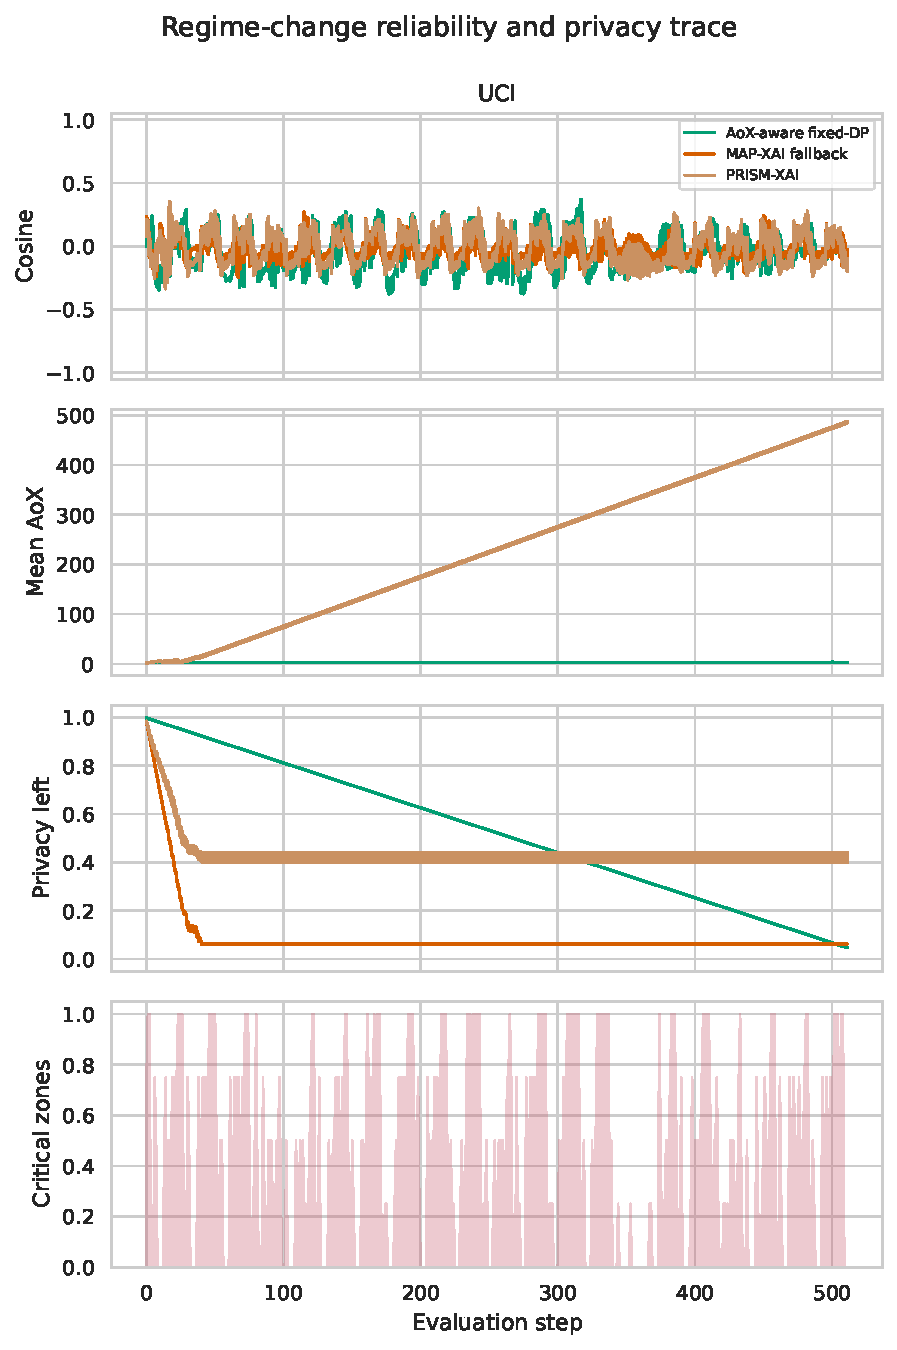
\includegraphics[width=.96\textwidth,height=.82\textheight,keepaspectratio]{../../SERVICE_TRADEOFF_RESULTS/runs/thr_1_cap_16/uci/regime_trace.pdf}

\caption{Public-score threshold $\tau=1$, release cap $M=16$, UCI: representative regime trace. This panel should be read with the setting-level quantitative interpretation and the complete tables immediately preceding the figure block.}

\end{figure*}

\clearpage

\begin{figure*}[p]

\centering

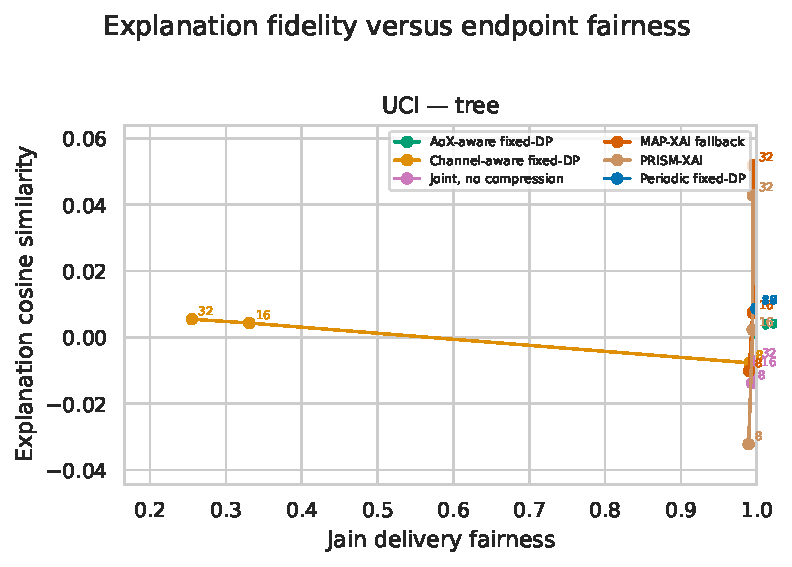
\includegraphics[width=.96\textwidth,height=.82\textheight,keepaspectratio]{../../SERVICE_TRADEOFF_RESULTS/runs/thr_1_cap_16/uci/fairness_reliability.pdf}

\caption{Public-score threshold $\tau=1$, release cap $M=16$, UCI: fairness--reliability plane. This panel should be read with the setting-level quantitative interpretation and the complete tables immediately preceding the figure block.}

\end{figure*}

\clearpage

\begin{figure*}[p]

\centering

\includegraphics[width=.96\textwidth,height=.82\textheight,keepaspectratio]{../../SERVICE_TRADEOFF_RESULTS/runs/thr_1_cap_16/uci/privacy_fidelity.pdf}

\caption{Public-score threshold $\tau=1$, release cap $M=16$, UCI: privacy--fidelity plane. This panel should be read with the setting-level quantitative interpretation and the complete tables immediately preceding the figure block.}

\end{figure*}

\clearpage

\begin{figure*}[p]

\centering

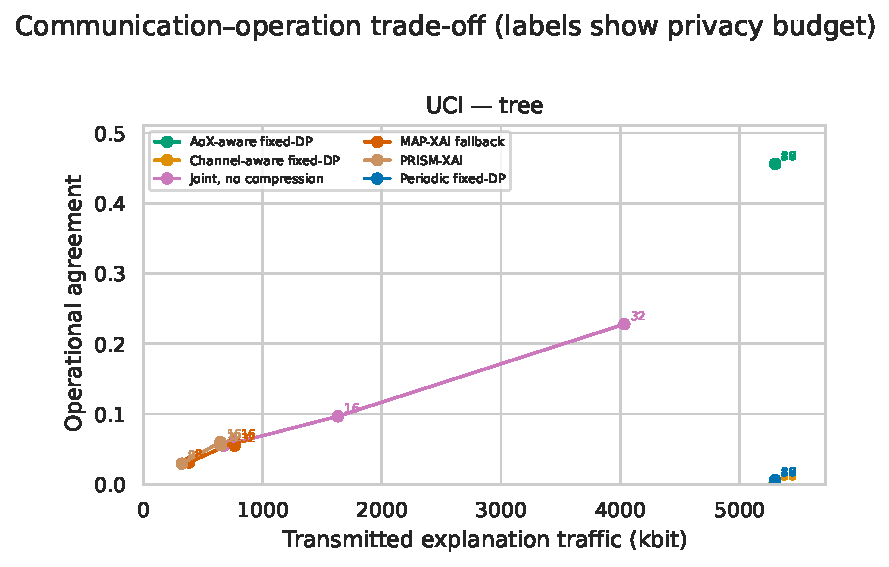
\includegraphics[width=.96\textwidth,height=.82\textheight,keepaspectratio]{../../SERVICE_TRADEOFF_RESULTS/runs/thr_1_cap_16/uci/pareto_bits_fidelity.pdf}

\caption{Public-score threshold $\tau=1$, release cap $M=16$, UCI: traffic--fidelity Pareto plane. This panel should be read with the setting-level quantitative interpretation and the complete tables immediately preceding the figure block.}

\end{figure*}

\clearpage

\begin{figure*}[p]

\centering

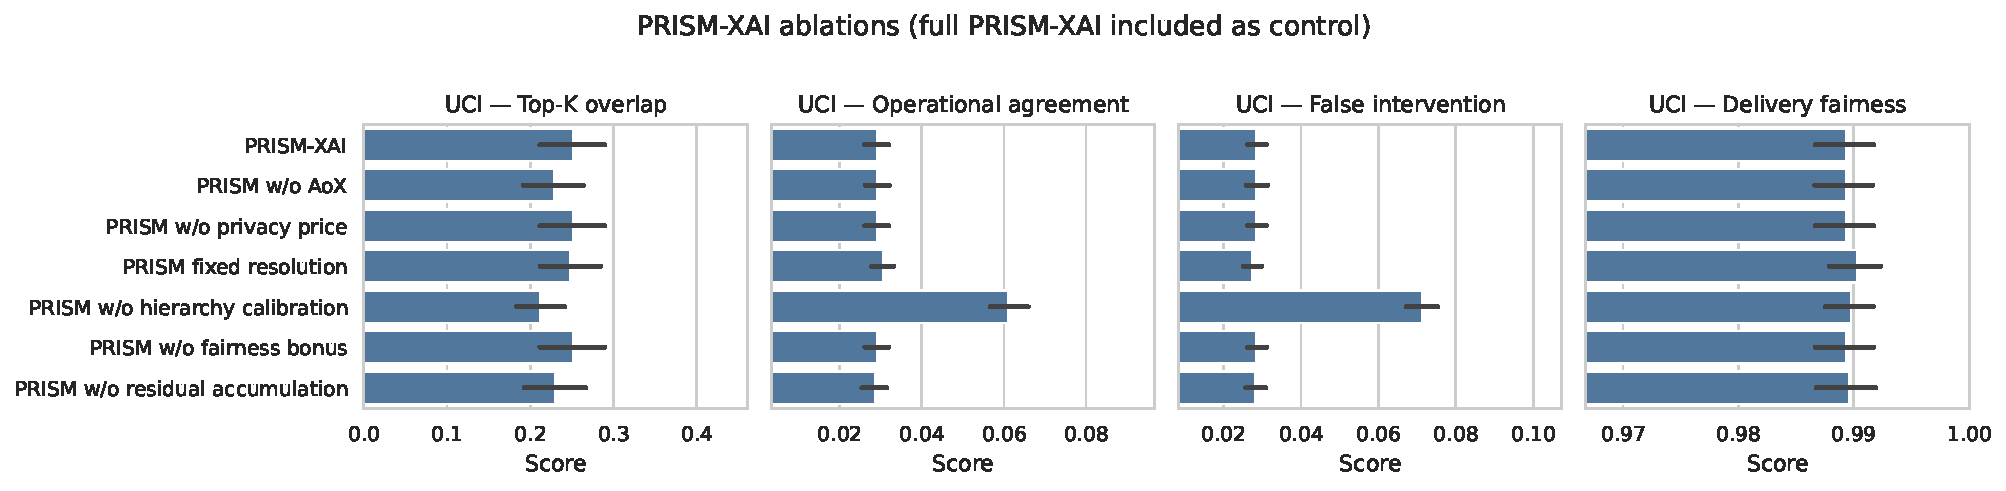
\includegraphics[width=.96\textwidth,height=.82\textheight,keepaspectratio]{../../SERVICE_TRADEOFF_RESULTS/runs/thr_1_cap_16/uci/ablation_results.pdf}

\caption{Public-score threshold $\tau=1$, release cap $M=16$, UCI: component ablation. This panel should be read with the setting-level quantitative interpretation and the complete tables immediately preceding the figure block.}

\end{figure*}

\clearpage

\subsubsection{Public-score threshold $\tau=2$, release cap $M=16$}

At this operating point, PRISM-XAI transmits 343.07~kbit versus 407.50~kbit for MAP-XAI-only (aggregate-mean ratio saving 15.81\%). The paired difference is -64.43$\pm$7.17~kbit. PRISM coverage is 0.1248, critical-event recall is 0.0594, and maximum recorded expenditure is 17.745. Relative to MAP-XAI-only, the paired coverage change is -0.00024$\pm$0.00023 and recall change is +0.00076$\pm$0.00208. The descriptive overlap rule holds in 8 of 12 cells. Accordingly, this point is read as a sensitivity point on the service frontier, not a complete matched-service confirmation.

\paragraph{Combined datasets.} The three generated tables below report the full method means, all condition-level values, and paired differences. The five figures that follow provide the corresponding temporal, fairness, privacy, Pareto, and ablation views. Aggregate panels support the setting-level summary above; dataset panels reveal whether that summary is shared by OPSD and UCI rather than being driven by their different endpoint counts.

\begin{table*}[p]\centering\tiny

\caption{Public-score threshold $\tau=2$, release cap $M=16$, Combined datasets: complete generated method table.}

\label{tab:thr_2_cap_16:combined:main}

\resizebox{\linewidth}{!}{% Values are means with 95% Student-t confidence intervals across seeds.
\begin{tabular}{lccccccccccccccc}
\toprule
Dataset & Model & $\epsilon_{\max}$ & Method & Top-$K$ & Cosine & Decision & Recall & Prec. & Abst. & P95 ms & kbit & Spent $\epsilon$ & False int. & bit/correct & Fairness \\
\midrule
OPSD & Tree & 8 & AoX-aware fixed-DP & 0.234 $\pm$ 0.048 & -0.033 $\pm$ 0.028 & 0.119 $\pm$ 0.028 & 0.119 $\pm$ 0.028 & 0.198 $\pm$ 0.054 & 0.721 $\pm$ 0.005 & 6.903 $\pm$ 1.126 & 1560.564 $\pm$ 0.000 & 7.990 $\pm$ 0.000 & 0.183 $\pm$ 0.020 & 35567.482 $\pm$ 10569.818 & 0.999 $\pm$ 0.000 \\
OPSD & Tree & 8 & AoX-aware fixed-DP & 0.238 $\pm$ 0.049 & -0.026 $\pm$ 0.055 & 0.121 $\pm$ 0.026 & 0.121 $\pm$ 0.026 & 0.205 $\pm$ 0.053 & 0.721 $\pm$ 0.005 & 6.903 $\pm$ 1.126 & 1560.564 $\pm$ 0.000 & 7.990 $\pm$ 0.000 & 0.179 $\pm$ 0.023 & 34123.214 $\pm$ 8376.542 & 0.999 $\pm$ 0.000 \\
OPSD & Tree & 8 & Channel-aware fixed-DP & 0.292 $\pm$ 0.037 & -0.041 $\pm$ 0.051 & 0.107 $\pm$ 0.026 & 0.107 $\pm$ 0.026 & 0.217 $\pm$ 0.068 & 0.779 $\pm$ 0.011 & 5.571 $\pm$ 1.784 & 1560.564 $\pm$ 0.000 & 7.990 $\pm$ 0.000 & 0.154 $\pm$ 0.029 & 40860.756 $\pm$ 14126.920 & 0.999 $\pm$ 0.000 \\
OPSD & Tree & 8 & Channel-aware fixed-DP & 0.292 $\pm$ 0.054 & -0.049 $\pm$ 0.064 & 0.111 $\pm$ 0.023 & 0.111 $\pm$ 0.023 & 0.228 $\pm$ 0.066 & 0.779 $\pm$ 0.011 & 5.571 $\pm$ 1.784 & 1560.564 $\pm$ 0.000 & 7.990 $\pm$ 0.000 & 0.149 $\pm$ 0.026 & 37980.855 $\pm$ 12338.094 & 0.999 $\pm$ 0.000 \\
OPSD & Tree & 8 & Joint, no compression & 0.288 $\pm$ 0.064 & -0.030 $\pm$ 0.079 & 0.016 $\pm$ 0.005 & 0.016 $\pm$ 0.005 & 0.193 $\pm$ 0.059 & 0.957 $\pm$ 0.003 & 4.560 $\pm$ 1.811 & 189.900 $\pm$ 0.554 & 7.990 $\pm$ 0.000 & 0.027 $\pm$ 0.005 & 32490.357 $\pm$ 10149.755 & 0.996 $\pm$ 0.002 \\
OPSD & Tree & 8 & Joint, no compression & 0.258 $\pm$ 0.055 & 0.011 $\pm$ 0.094 & 0.019 $\pm$ 0.004 & 0.019 $\pm$ 0.004 & 0.224 $\pm$ 0.044 & 0.957 $\pm$ 0.003 & 4.562 $\pm$ 1.809 & 189.750 $\pm$ 0.566 & 7.990 $\pm$ 0.000 & 0.025 $\pm$ 0.003 & 26079.167 $\pm$ 6335.386 & 0.996 $\pm$ 0.002 \\
OPSD & Tree & 8 & Periodic fixed-DP & 0.241 $\pm$ 0.049 & -0.019 $\pm$ 0.061 & 0.125 $\pm$ 0.020 & 0.125 $\pm$ 0.020 & 0.209 $\pm$ 0.044 & 0.722 $\pm$ 0.006 & 6.303 $\pm$ 1.438 & 1560.564 $\pm$ 0.000 & 7.990 $\pm$ 0.000 & 0.181 $\pm$ 0.021 & 31183.082 $\pm$ 4356.378 & 0.999 $\pm$ 0.000 \\
OPSD & Tree & 8 & Periodic fixed-DP & 0.242 $\pm$ 0.048 & -0.026 $\pm$ 0.082 & 0.135 $\pm$ 0.016 & 0.135 $\pm$ 0.016 & 0.231 $\pm$ 0.037 & 0.722 $\pm$ 0.006 & 6.303 $\pm$ 1.438 & 1560.564 $\pm$ 0.000 & 7.990 $\pm$ 0.000 & 0.169 $\pm$ 0.017 & 28520.235 $\pm$ 3511.595 & 0.999 $\pm$ 0.000 \\
OPSD & Tree & 8 & PRISM-XAI & 0.170 $\pm$ 0.039 & 0.027 $\pm$ 0.072 & 0.029 $\pm$ 0.012 & 0.029 $\pm$ 0.012 & 0.326 $\pm$ 0.147 & 0.938 $\pm$ 0.004 & 4.881 $\pm$ 1.730 & 88.137 $\pm$ 0.577 & 6.066 $\pm$ 0.239 & 0.024 $\pm$ 0.007 & 10754.619 $\pm$ 5615.749 & 0.991 $\pm$ 0.006 \\
OPSD & Tree & 8 & PRISM-XAI & 0.171 $\pm$ 0.046 & 0.026 $\pm$ 0.082 & 0.031 $\pm$ 0.010 & 0.031 $\pm$ 0.010 & 0.343 $\pm$ 0.130 & 0.938 $\pm$ 0.004 & 4.873 $\pm$ 1.737 & 87.707 $\pm$ 0.532 & 5.936 $\pm$ 0.213 & 0.024 $\pm$ 0.007 & 8388.650 $\pm$ 2960.712 & 0.991 $\pm$ 0.006 \\
OPSD & Tree & 8 & MAP-XAI fallback & 0.203 $\pm$ 0.058 & 0.019 $\pm$ 0.075 & 0.029 $\pm$ 0.011 & 0.029 $\pm$ 0.011 & 0.324 $\pm$ 0.148 & 0.938 $\pm$ 0.004 & 4.960 $\pm$ 1.678 & 105.889 $\pm$ 0.169 & 7.786 $\pm$ 0.000 & 0.026 $\pm$ 0.008 & 11344.761 $\pm$ 4319.900 & 0.991 $\pm$ 0.006 \\
OPSD & Tree & 8 & MAP-XAI fallback & 0.181 $\pm$ 0.054 & 0.025 $\pm$ 0.081 & 0.029 $\pm$ 0.009 & 0.029 $\pm$ 0.009 & 0.310 $\pm$ 0.118 & 0.938 $\pm$ 0.004 & 4.960 $\pm$ 1.678 & 105.737 $\pm$ 0.152 & 7.786 $\pm$ 0.000 & 0.026 $\pm$ 0.007 & 10402.432 $\pm$ 2994.804 & 0.991 $\pm$ 0.006 \\
UCI & Tree & 8 & AoX-aware fixed-DP & 0.263 $\pm$ 0.041 & -0.007 $\pm$ 0.009 & 0.457 $\pm$ 0.031 & 0.457 $\pm$ 0.031 & 0.362 $\pm$ 0.024 & 0.003 $\pm$ 0.001 & 7.500 $\pm$ 0.000 & 5300.224 $\pm$ 0.000 & 7.990 $\pm$ 0.000 & 0.557 $\pm$ 0.025 & 14002.896 $\pm$ 1040.243 & 0.999 $\pm$ 0.000 \\
UCI & Tree & 8 & AoX-aware fixed-DP & 0.260 $\pm$ 0.022 & 0.010 $\pm$ 0.055 & 0.455 $\pm$ 0.047 & 0.455 $\pm$ 0.047 & 0.361 $\pm$ 0.038 & 0.003 $\pm$ 0.001 & 7.500 $\pm$ 0.000 & 5300.224 $\pm$ 0.000 & 7.990 $\pm$ 0.000 & 0.557 $\pm$ 0.048 & 14198.303 $\pm$ 1508.274 & 0.999 $\pm$ 0.000 \\
UCI & Tree & 8 & Channel-aware fixed-DP & 0.248 $\pm$ 0.031 & 0.004 $\pm$ 0.012 & 0.001 $\pm$ 0.001 & 0.001 $\pm$ 0.001 & 0.150 $\pm$ 0.151 & 0.999 $\pm$ 0.001 & 4.609 $\pm$ 1.781 & 5295.177 $\pm$ 3.740 & 7.990 $\pm$ 0.000 & 0.001 $\pm$ 0.001 & 4632196.500 $\pm$ 2102650.252 & 0.991 $\pm$ 0.001 \\
UCI & Tree & 8 & Channel-aware fixed-DP & 0.239 $\pm$ 0.030 & -0.020 $\pm$ 0.055 & 0.000 $\pm$ 0.000 & 0.000 $\pm$ 0.000 & 0.117 $\pm$ 0.225 & 0.999 $\pm$ 0.001 & 4.609 $\pm$ 1.781 & 5295.177 $\pm$ 3.740 & 7.990 $\pm$ 0.000 & 0.001 $\pm$ 0.001 & 5296989.000 $\pm$ 41104.572 & 0.991 $\pm$ 0.001 \\
UCI & Tree & 8 & Joint, no compression & 0.286 $\pm$ 0.045 & 0.004 $\pm$ 0.020 & 0.052 $\pm$ 0.005 & 0.052 $\pm$ 0.005 & 0.406 $\pm$ 0.037 & 0.875 $\pm$ 0.003 & 5.123 $\pm$ 1.792 & 672.300 $\pm$ 0.452 & 7.990 $\pm$ 0.000 & 0.053 $\pm$ 0.004 & 15676.175 $\pm$ 1475.621 & 0.994 $\pm$ 0.003 \\
UCI & Tree & 8 & Joint, no compression & 0.229 $\pm$ 0.052 & -0.032 $\pm$ 0.050 & 0.057 $\pm$ 0.007 & 0.057 $\pm$ 0.007 & 0.428 $\pm$ 0.041 & 0.875 $\pm$ 0.003 & 5.131 $\pm$ 1.787 & 672.300 $\pm$ 0.452 & 7.990 $\pm$ 0.000 & 0.052 $\pm$ 0.004 & 14702.786 $\pm$ 2334.488 & 0.994 $\pm$ 0.003 \\
UCI & Tree & 8 & Periodic fixed-DP & 0.259 $\pm$ 0.060 & -0.005 $\pm$ 0.008 & 0.006 $\pm$ 0.001 & 0.006 $\pm$ 0.001 & 0.244 $\pm$ 0.049 & 0.989 $\pm$ 0.001 & 4.596 $\pm$ 1.788 & 5299.318 $\pm$ 1.451 & 7.786 $\pm$ 0.000 & 0.013 $\pm$ 0.002 & 1215103.896 $\pm$ 390671.319 & 0.999 $\pm$ 0.000 \\
UCI & Tree & 8 & Periodic fixed-DP & 0.260 $\pm$ 0.044 & 0.022 $\pm$ 0.070 & 0.005 $\pm$ 0.001 & 0.005 $\pm$ 0.001 & 0.195 $\pm$ 0.050 & 0.989 $\pm$ 0.001 & 4.596 $\pm$ 1.788 & 5299.318 $\pm$ 1.451 & 7.786 $\pm$ 0.000 & 0.015 $\pm$ 0.002 & 1555837.203 $\pm$ 955472.503 & 0.999 $\pm$ 0.000 \\
UCI & Tree & 8 & PRISM-XAI & 0.220 $\pm$ 0.061 & -0.009 $\pm$ 0.015 & 0.045 $\pm$ 0.006 & 0.045 $\pm$ 0.006 & 0.442 $\pm$ 0.072 & 0.906 $\pm$ 0.004 & 4.504 $\pm$ 1.537 & 325.842 $\pm$ 1.091 & 6.877 $\pm$ 0.090 & 0.040 $\pm$ 0.007 & 8917.519 $\pm$ 1309.048 & 0.992 $\pm$ 0.002 \\
UCI & Tree & 8 & PRISM-XAI & 0.217 $\pm$ 0.043 & -0.008 $\pm$ 0.077 & 0.045 $\pm$ 0.007 & 0.045 $\pm$ 0.007 & 0.447 $\pm$ 0.078 & 0.908 $\pm$ 0.002 & 5.058 $\pm$ 1.846 & 322.524 $\pm$ 0.793 & 6.877 $\pm$ 0.090 & 0.039 $\pm$ 0.008 & 9128.968 $\pm$ 1604.303 & 0.991 $\pm$ 0.004 \\
UCI & Tree & 8 & MAP-XAI fallback & 0.155 $\pm$ 0.082 & 0.000 $\pm$ 0.016 & 0.047 $\pm$ 0.007 & 0.047 $\pm$ 0.007 & 0.456 $\pm$ 0.051 & 0.905 $\pm$ 0.004 & 4.584 $\pm$ 1.508 & 381.745 $\pm$ 0.387 & 7.787 $\pm$ 0.001 & 0.038 $\pm$ 0.003 & 10122.948 $\pm$ 1695.832 & 0.992 $\pm$ 0.002 \\
UCI & Tree & 8 & MAP-XAI fallback & 0.221 $\pm$ 0.054 & 0.040 $\pm$ 0.080 & 0.046 $\pm$ 0.008 & 0.046 $\pm$ 0.008 & 0.469 $\pm$ 0.072 & 0.907 $\pm$ 0.003 & 4.763 $\pm$ 1.714 & 381.283 $\pm$ 0.251 & 7.787 $\pm$ 0.001 & 0.036 $\pm$ 0.006 & 10525.744 $\pm$ 1825.173 & 0.991 $\pm$ 0.004 \\
\bottomrule
\end{tabular}
}

\end{table*}\clearpage

\begin{table*}[p]\centering\tiny

\caption{Public-score threshold $\tau=2$, release cap $M=16$, Combined datasets: complete condition-level generated table.}

\label{tab:thr_2_cap_16:combined:conditions}

\resizebox{\textwidth}{!}{\begin{tabular}{llllccccccccccc}
\toprule
Dataset & Model & $\epsilon_{\max}$ & Method & kbit & Top-$K$ & Random Top-$K$ & Cosine & Decision & Recall & Precision & Coverage & Abstain & False int. & Spent $\epsilon$ \\
\midrule
OPSD & Tree & 8 & Joint, no compression & 189.900 $\pm$ 0.554 & 0.288 $\pm$ 0.064 & 0.250 $\pm$ 0.000 & -0.030 $\pm$ 0.079 & 0.016 $\pm$ 0.005 & 0.016 $\pm$ 0.005 & 0.193 $\pm$ 0.059 & 0.043 $\pm$ 0.003 & 0.957 $\pm$ 0.003 & 0.027 $\pm$ 0.005 & 7.990 $\pm$ 0.000 \\
OPSD & Tree & 8 & Joint, no compression & 189.750 $\pm$ 0.566 & 0.258 $\pm$ 0.055 & 0.250 $\pm$ 0.000 & 0.011 $\pm$ 0.094 & 0.019 $\pm$ 0.004 & 0.019 $\pm$ 0.004 & 0.224 $\pm$ 0.044 & 0.043 $\pm$ 0.003 & 0.957 $\pm$ 0.003 & 0.025 $\pm$ 0.003 & 7.990 $\pm$ 0.000 \\
OPSD & Tree & 8 & Periodic fixed-DP & 1560.564 $\pm$ 0.000 & 0.241 $\pm$ 0.049 & 0.250 $\pm$ 0.000 & -0.019 $\pm$ 0.061 & 0.125 $\pm$ 0.020 & 0.125 $\pm$ 0.020 & 0.209 $\pm$ 0.044 & 0.278 $\pm$ 0.006 & 0.722 $\pm$ 0.006 & 0.181 $\pm$ 0.021 & 7.990 $\pm$ 0.000 \\
OPSD & Tree & 8 & Periodic fixed-DP & 1560.564 $\pm$ 0.000 & 0.242 $\pm$ 0.048 & 0.250 $\pm$ 0.000 & -0.026 $\pm$ 0.082 & 0.135 $\pm$ 0.016 & 0.135 $\pm$ 0.016 & 0.231 $\pm$ 0.037 & 0.278 $\pm$ 0.006 & 0.722 $\pm$ 0.006 & 0.169 $\pm$ 0.017 & 7.990 $\pm$ 0.000 \\
OPSD & Tree & 8 & PRISM-XAI & 88.137 $\pm$ 0.577 & 0.170 $\pm$ 0.039 & 0.250 $\pm$ 0.000 & 0.027 $\pm$ 0.072 & 0.029 $\pm$ 0.012 & 0.029 $\pm$ 0.012 & 0.326 $\pm$ 0.147 & 0.062 $\pm$ 0.004 & 0.938 $\pm$ 0.004 & 0.024 $\pm$ 0.007 & 6.066 $\pm$ 0.239 \\
OPSD & Tree & 8 & PRISM-XAI & 87.707 $\pm$ 0.532 & 0.171 $\pm$ 0.046 & 0.250 $\pm$ 0.000 & 0.026 $\pm$ 0.082 & 0.031 $\pm$ 0.010 & 0.031 $\pm$ 0.010 & 0.343 $\pm$ 0.130 & 0.062 $\pm$ 0.004 & 0.938 $\pm$ 0.004 & 0.024 $\pm$ 0.007 & 5.936 $\pm$ 0.213 \\
OPSD & Tree & 16 & Joint, no compression & 459.900 $\pm$ 0.750 & 0.232 $\pm$ 0.065 & 0.250 $\pm$ 0.000 & 0.059 $\pm$ 0.048 & 0.038 $\pm$ 0.009 & 0.038 $\pm$ 0.009 & 0.222 $\pm$ 0.049 & 0.088 $\pm$ 0.004 & 0.912 $\pm$ 0.004 & 0.049 $\pm$ 0.005 & 15.997 $\pm$ 0.000 \\
OPSD & Tree & 16 & Joint, no compression & 460.050 $\pm$ 0.724 & 0.241 $\pm$ 0.055 & 0.250 $\pm$ 0.000 & 0.061 $\pm$ 0.052 & 0.039 $\pm$ 0.008 & 0.039 $\pm$ 0.008 & 0.241 $\pm$ 0.042 & 0.088 $\pm$ 0.004 & 0.912 $\pm$ 0.004 & 0.045 $\pm$ 0.004 & 15.997 $\pm$ 0.000 \\
OPSD & Tree & 16 & Periodic fixed-DP & 5112.594 $\pm$ 0.000 & 0.249 $\pm$ 0.022 & 0.250 $\pm$ 0.000 & -0.009 $\pm$ 0.045 & 0.450 $\pm$ 0.062 & 0.450 $\pm$ 0.062 & 0.237 $\pm$ 0.042 & 0.985 $\pm$ 0.002 & 0.015 $\pm$ 0.002 & 0.551 $\pm$ 0.057 & 15.997 $\pm$ 0.000 \\
OPSD & Tree & 16 & Periodic fixed-DP & 5112.594 $\pm$ 0.000 & 0.243 $\pm$ 0.019 & 0.250 $\pm$ 0.000 & -0.012 $\pm$ 0.050 & 0.463 $\pm$ 0.047 & 0.463 $\pm$ 0.047 & 0.240 $\pm$ 0.028 & 0.985 $\pm$ 0.002 & 0.015 $\pm$ 0.002 & 0.547 $\pm$ 0.036 & 15.997 $\pm$ 0.000 \\
OPSD & Tree & 16 & PRISM-XAI & 176.428 $\pm$ 0.771 & 0.259 $\pm$ 0.050 & 0.250 $\pm$ 0.000 & 0.054 $\pm$ 0.064 & 0.053 $\pm$ 0.015 & 0.053 $\pm$ 0.015 & 0.339 $\pm$ 0.133 & 0.120 $\pm$ 0.006 & 0.880 $\pm$ 0.006 & 0.042 $\pm$ 0.011 & 15.620 $\pm$ 0.000 \\
OPSD & Tree & 16 & PRISM-XAI & 175.629 $\pm$ 0.704 & 0.256 $\pm$ 0.054 & 0.250 $\pm$ 0.000 & 0.071 $\pm$ 0.073 & 0.050 $\pm$ 0.013 & 0.050 $\pm$ 0.013 & 0.291 $\pm$ 0.104 & 0.120 $\pm$ 0.006 & 0.880 $\pm$ 0.006 & 0.049 $\pm$ 0.010 & 15.620 $\pm$ 0.000 \\
OPSD & Tree & 32 & Joint, no compression & 1140.900 $\pm$ 7.953 & 0.235 $\pm$ 0.064 & 0.250 $\pm$ 0.000 & -0.031 $\pm$ 0.089 & 0.074 $\pm$ 0.015 & 0.074 $\pm$ 0.015 & 0.205 $\pm$ 0.039 & 0.157 $\pm$ 0.006 & 0.843 $\pm$ 0.006 & 0.107 $\pm$ 0.009 & 31.999 $\pm$ 0.000 \\
OPSD & Tree & 32 & Joint, no compression & 1140.900 $\pm$ 7.953 & 0.282 $\pm$ 0.054 & 0.250 $\pm$ 0.000 & -0.044 $\pm$ 0.076 & 0.080 $\pm$ 0.011 & 0.080 $\pm$ 0.011 & 0.227 $\pm$ 0.052 & 0.158 $\pm$ 0.006 & 0.842 $\pm$ 0.006 & 0.105 $\pm$ 0.015 & 31.999 $\pm$ 0.000 \\
OPSD & Tree & 32 & Periodic fixed-DP & 5299.836 $\pm$ 0.625 & 0.249 $\pm$ 0.022 & 0.250 $\pm$ 0.000 & -0.009 $\pm$ 0.044 & 0.458 $\pm$ 0.066 & 0.458 $\pm$ 0.066 & 0.237 $\pm$ 0.045 & 1.000 $\pm$ 0.000 & 0.000 $\pm$ 0.000 & 0.562 $\pm$ 0.062 & 16.371 $\pm$ 0.000 \\
OPSD & Tree & 32 & Periodic fixed-DP & 5299.836 $\pm$ 0.625 & 0.244 $\pm$ 0.019 & 0.250 $\pm$ 0.000 & -0.012 $\pm$ 0.050 & 0.471 $\pm$ 0.049 & 0.471 $\pm$ 0.049 & 0.240 $\pm$ 0.029 & 1.000 $\pm$ 0.000 & 0.000 $\pm$ 0.000 & 0.559 $\pm$ 0.039 & 16.371 $\pm$ 0.000 \\
OPSD & Tree & 32 & PRISM-XAI & 176.336 $\pm$ 0.759 & 0.315 $\pm$ 0.088 & 0.250 $\pm$ 0.000 & 0.193 $\pm$ 0.062 & 0.061 $\pm$ 0.013 & 0.061 $\pm$ 0.013 & 0.397 $\pm$ 0.114 & 0.120 $\pm$ 0.006 & 0.880 $\pm$ 0.006 & 0.037 $\pm$ 0.010 & 31.175 $\pm$ 0.000 \\
OPSD & Tree & 32 & PRISM-XAI & 175.415 $\pm$ 0.593 & 0.314 $\pm$ 0.062 & 0.250 $\pm$ 0.000 & 0.240 $\pm$ 0.062 & 0.060 $\pm$ 0.013 & 0.060 $\pm$ 0.013 & 0.365 $\pm$ 0.089 & 0.120 $\pm$ 0.006 & 0.880 $\pm$ 0.006 & 0.040 $\pm$ 0.008 & 31.175 $\pm$ 0.000 \\
UCI & Tree & 8 & Joint, no compression & 672.300 $\pm$ 0.452 & 0.286 $\pm$ 0.045 & 0.250 $\pm$ 0.000 & 0.004 $\pm$ 0.020 & 0.052 $\pm$ 0.005 & 0.052 $\pm$ 0.005 & 0.406 $\pm$ 0.037 & 0.125 $\pm$ 0.003 & 0.875 $\pm$ 0.003 & 0.053 $\pm$ 0.004 & 7.990 $\pm$ 0.000 \\
UCI & Tree & 8 & Joint, no compression & 672.300 $\pm$ 0.452 & 0.229 $\pm$ 0.052 & 0.250 $\pm$ 0.000 & -0.032 $\pm$ 0.050 & 0.057 $\pm$ 0.007 & 0.057 $\pm$ 0.007 & 0.428 $\pm$ 0.041 & 0.125 $\pm$ 0.003 & 0.875 $\pm$ 0.003 & 0.052 $\pm$ 0.004 & 7.990 $\pm$ 0.000 \\
UCI & Tree & 8 & Periodic fixed-DP & 5299.318 $\pm$ 1.451 & 0.259 $\pm$ 0.060 & 0.250 $\pm$ 0.000 & -0.005 $\pm$ 0.008 & 0.006 $\pm$ 0.001 & 0.006 $\pm$ 0.001 & 0.244 $\pm$ 0.049 & 0.011 $\pm$ 0.001 & 0.989 $\pm$ 0.001 & 0.013 $\pm$ 0.002 & 7.786 $\pm$ 0.000 \\
UCI & Tree & 8 & Periodic fixed-DP & 5299.318 $\pm$ 1.451 & 0.260 $\pm$ 0.044 & 0.250 $\pm$ 0.000 & 0.022 $\pm$ 0.070 & 0.005 $\pm$ 0.001 & 0.005 $\pm$ 0.001 & 0.195 $\pm$ 0.050 & 0.011 $\pm$ 0.001 & 0.989 $\pm$ 0.001 & 0.015 $\pm$ 0.002 & 7.786 $\pm$ 0.000 \\
UCI & Tree & 8 & PRISM-XAI & 325.842 $\pm$ 1.091 & 0.220 $\pm$ 0.061 & 0.250 $\pm$ 0.000 & -0.009 $\pm$ 0.015 & 0.045 $\pm$ 0.006 & 0.045 $\pm$ 0.006 & 0.442 $\pm$ 0.072 & 0.094 $\pm$ 0.004 & 0.906 $\pm$ 0.004 & 0.040 $\pm$ 0.007 & 6.877 $\pm$ 0.090 \\
UCI & Tree & 8 & PRISM-XAI & 322.524 $\pm$ 0.793 & 0.217 $\pm$ 0.043 & 0.250 $\pm$ 0.000 & -0.008 $\pm$ 0.077 & 0.045 $\pm$ 0.007 & 0.045 $\pm$ 0.007 & 0.447 $\pm$ 0.078 & 0.092 $\pm$ 0.002 & 0.908 $\pm$ 0.002 & 0.039 $\pm$ 0.008 & 6.877 $\pm$ 0.090 \\
UCI & Tree & 16 & Joint, no compression & 1632.150 $\pm$ 0.339 & 0.216 $\pm$ 0.041 & 0.250 $\pm$ 0.000 & 0.001 $\pm$ 0.012 & 0.094 $\pm$ 0.005 & 0.094 $\pm$ 0.005 & 0.330 $\pm$ 0.024 & 0.228 $\pm$ 0.005 & 0.772 $\pm$ 0.005 & 0.133 $\pm$ 0.010 & 15.997 $\pm$ 0.000 \\
UCI & Tree & 16 & Joint, no compression & 1632.600 $\pm$ 0.554 & 0.204 $\pm$ 0.011 & 0.250 $\pm$ 0.000 & -0.021 $\pm$ 0.033 & 0.099 $\pm$ 0.016 & 0.099 $\pm$ 0.016 & 0.347 $\pm$ 0.054 & 0.228 $\pm$ 0.005 & 0.772 $\pm$ 0.005 & 0.128 $\pm$ 0.011 & 15.997 $\pm$ 0.000 \\
UCI & Tree & 16 & Periodic fixed-DP & 5299.318 $\pm$ 1.451 & 0.259 $\pm$ 0.060 & 0.250 $\pm$ 0.000 & -0.005 $\pm$ 0.008 & 0.006 $\pm$ 0.001 & 0.006 $\pm$ 0.001 & 0.244 $\pm$ 0.049 & 0.011 $\pm$ 0.001 & 0.989 $\pm$ 0.001 & 0.013 $\pm$ 0.002 & 7.786 $\pm$ 0.000 \\
UCI & Tree & 16 & Periodic fixed-DP & 5299.318 $\pm$ 1.451 & 0.260 $\pm$ 0.044 & 0.250 $\pm$ 0.000 & 0.022 $\pm$ 0.070 & 0.005 $\pm$ 0.001 & 0.005 $\pm$ 0.001 & 0.195 $\pm$ 0.050 & 0.011 $\pm$ 0.001 & 0.989 $\pm$ 0.001 & 0.015 $\pm$ 0.002 & 7.786 $\pm$ 0.000 \\
UCI & Tree & 16 & PRISM-XAI & 650.843 $\pm$ 1.226 & 0.297 $\pm$ 0.062 & 0.250 $\pm$ 0.000 & 0.008 $\pm$ 0.020 & 0.087 $\pm$ 0.008 & 0.087 $\pm$ 0.008 & 0.454 $\pm$ 0.046 & 0.180 $\pm$ 0.003 & 0.820 $\pm$ 0.003 & 0.073 $\pm$ 0.007 & 15.620 $\pm$ 0.000 \\
UCI & Tree & 16 & PRISM-XAI & 644.135 $\pm$ 1.590 & 0.251 $\pm$ 0.053 & 0.250 $\pm$ 0.000 & 0.011 $\pm$ 0.046 & 0.084 $\pm$ 0.009 & 0.084 $\pm$ 0.009 & 0.463 $\pm$ 0.061 & 0.177 $\pm$ 0.004 & 0.823 $\pm$ 0.004 & 0.069 $\pm$ 0.011 & 15.620 $\pm$ 0.000 \\
UCI & Tree & 32 & Joint, no compression & 4034.550 $\pm$ 5.034 & 0.246 $\pm$ 0.031 & 0.250 $\pm$ 0.000 & -0.002 $\pm$ 0.015 & 0.228 $\pm$ 0.013 & 0.228 $\pm$ 0.013 & 0.361 $\pm$ 0.028 & 0.537 $\pm$ 0.009 & 0.463 $\pm$ 0.009 & 0.279 $\pm$ 0.017 & 31.999 $\pm$ 0.000 \\
UCI & Tree & 32 & Joint, no compression & 4034.550 $\pm$ 5.034 & 0.241 $\pm$ 0.033 & 0.250 $\pm$ 0.000 & -0.012 $\pm$ 0.030 & 0.228 $\pm$ 0.028 & 0.228 $\pm$ 0.028 & 0.360 $\pm$ 0.047 & 0.530 $\pm$ 0.010 & 0.470 $\pm$ 0.010 & 0.280 $\pm$ 0.026 & 31.999 $\pm$ 0.000 \\
UCI & Tree & 32 & Periodic fixed-DP & 5299.318 $\pm$ 1.451 & 0.259 $\pm$ 0.060 & 0.250 $\pm$ 0.000 & -0.005 $\pm$ 0.008 & 0.006 $\pm$ 0.001 & 0.006 $\pm$ 0.001 & 0.244 $\pm$ 0.049 & 0.011 $\pm$ 0.001 & 0.989 $\pm$ 0.001 & 0.013 $\pm$ 0.002 & 7.786 $\pm$ 0.000 \\
UCI & Tree & 32 & Periodic fixed-DP & 5299.318 $\pm$ 1.451 & 0.260 $\pm$ 0.044 & 0.250 $\pm$ 0.000 & 0.022 $\pm$ 0.070 & 0.005 $\pm$ 0.001 & 0.005 $\pm$ 0.001 & 0.195 $\pm$ 0.050 & 0.011 $\pm$ 0.001 & 0.989 $\pm$ 0.001 & 0.015 $\pm$ 0.002 & 7.786 $\pm$ 0.000 \\
UCI & Tree & 32 & PRISM-XAI & 649.871 $\pm$ 1.443 & 0.332 $\pm$ 0.056 & 0.250 $\pm$ 0.000 & 0.010 $\pm$ 0.024 & 0.085 $\pm$ 0.007 & 0.085 $\pm$ 0.007 & 0.572 $\pm$ 0.040 & 0.177 $\pm$ 0.004 & 0.823 $\pm$ 0.004 & 0.044 $\pm$ 0.006 & 31.175 $\pm$ 0.000 \\
UCI & Tree & 32 & PRISM-XAI & 644.002 $\pm$ 1.573 & 0.310 $\pm$ 0.057 & 0.250 $\pm$ 0.000 & 0.016 $\pm$ 0.064 & 0.083 $\pm$ 0.012 & 0.083 $\pm$ 0.012 & 0.561 $\pm$ 0.063 & 0.173 $\pm$ 0.006 & 0.827 $\pm$ 0.006 & 0.045 $\pm$ 0.010 & 31.175 $\pm$ 0.000 \\
\bottomrule
\end{tabular}
}

\end{table*}\clearpage

\begin{table*}[p]\centering\tiny

\caption{Public-score threshold $\tau=2$, release cap $M=16$, Combined datasets: complete generated paired comparisons.}

\label{tab:thr_2_cap_16:combined:paired}

\resizebox{\textwidth}{!}{\begin{tabular}{llcccc}
\toprule
Dataset & Baseline & Delta kbit & Delta Top-$K$ & Delta recall & Delta fairness \\
\midrule
OPSD & AoX-aware fixed-DP & -1472.427 $\pm$ 0.577 & -0.064 $\pm$ 0.057 & -0.091 $\pm$ 0.033 & -0.008 $\pm$ 0.006 \\
OPSD & AoX-aware fixed-DP & -4923.485 $\pm$ 5.595 & 0.006 $\pm$ 0.053 & -0.349 $\pm$ 0.082 & -0.004 $\pm$ 0.002 \\
OPSD & AoX-aware fixed-DP & -5123.888 $\pm$ 0.759 & 0.062 $\pm$ 0.093 & -0.351 $\pm$ 0.083 & -0.004 $\pm$ 0.002 \\
OPSD & AoX-aware fixed-DP & -1472.857 $\pm$ 0.532 & -0.068 $\pm$ 0.063 & -0.090 $\pm$ 0.028 & -0.008 $\pm$ 0.006 \\
OPSD & AoX-aware fixed-DP & -4924.283 $\pm$ 5.582 & 0.004 $\pm$ 0.062 & -0.364 $\pm$ 0.062 & -0.004 $\pm$ 0.002 \\
OPSD & AoX-aware fixed-DP & -5124.809 $\pm$ 0.593 & 0.062 $\pm$ 0.071 & -0.366 $\pm$ 0.060 & -0.004 $\pm$ 0.002 \\
OPSD & Channel-aware fixed-DP & -1472.427 $\pm$ 0.577 & -0.122 $\pm$ 0.049 & -0.078 $\pm$ 0.029 & -0.008 $\pm$ 0.006 \\
OPSD & Channel-aware fixed-DP & -4510.181 $\pm$ 12.999 & -0.002 $\pm$ 0.048 & -0.349 $\pm$ 0.095 & 0.058 $\pm$ 0.005 \\
OPSD & Channel-aware fixed-DP & -5123.888 $\pm$ 0.759 & 0.057 $\pm$ 0.093 & -0.373 $\pm$ 0.102 & 0.089 $\pm$ 0.006 \\
OPSD & Channel-aware fixed-DP & -1472.857 $\pm$ 0.532 & -0.122 $\pm$ 0.074 & -0.080 $\pm$ 0.025 & -0.008 $\pm$ 0.006 \\
OPSD & Channel-aware fixed-DP & -4510.980 $\pm$ 13.099 & -0.002 $\pm$ 0.051 & -0.369 $\pm$ 0.093 & 0.058 $\pm$ 0.005 \\
OPSD & Channel-aware fixed-DP & -5124.809 $\pm$ 0.593 & 0.057 $\pm$ 0.070 & -0.396 $\pm$ 0.090 & 0.089 $\pm$ 0.006 \\
OPSD & Joint, no compression & -101.763 $\pm$ 0.687 & -0.118 $\pm$ 0.078 & 0.012 $\pm$ 0.011 & -0.005 $\pm$ 0.005 \\
OPSD & Joint, no compression & -283.472 $\pm$ 1.424 & 0.028 $\pm$ 0.096 & 0.015 $\pm$ 0.017 & -0.002 $\pm$ 0.002 \\
OPSD & Joint, no compression & -964.564 $\pm$ 8.170 & 0.080 $\pm$ 0.106 & -0.013 $\pm$ 0.022 & -0.003 $\pm$ 0.002 \\
OPSD & Joint, no compression & -102.043 $\pm$ 0.513 & -0.088 $\pm$ 0.080 & 0.012 $\pm$ 0.009 & -0.005 $\pm$ 0.005 \\
OPSD & Joint, no compression & -284.421 $\pm$ 1.294 & 0.015 $\pm$ 0.063 & 0.011 $\pm$ 0.014 & -0.002 $\pm$ 0.002 \\
OPSD & Joint, no compression & -965.485 $\pm$ 8.153 & 0.032 $\pm$ 0.101 & -0.020 $\pm$ 0.016 & -0.003 $\pm$ 0.002 \\
OPSD & Periodic fixed-DP & -1472.427 $\pm$ 0.577 & -0.070 $\pm$ 0.050 & -0.096 $\pm$ 0.024 & -0.008 $\pm$ 0.006 \\
OPSD & Periodic fixed-DP & -4936.166 $\pm$ 0.771 & 0.010 $\pm$ 0.060 & -0.398 $\pm$ 0.067 & -0.004 $\pm$ 0.002 \\
OPSD & Periodic fixed-DP & -5123.500 $\pm$ 0.672 & 0.066 $\pm$ 0.097 & -0.397 $\pm$ 0.070 & -0.004 $\pm$ 0.002 \\
OPSD & Periodic fixed-DP & -1472.857 $\pm$ 0.532 & -0.071 $\pm$ 0.050 & -0.104 $\pm$ 0.018 & -0.008 $\pm$ 0.006 \\
OPSD & Periodic fixed-DP & -4936.965 $\pm$ 0.704 & 0.013 $\pm$ 0.062 & -0.412 $\pm$ 0.051 & -0.004 $\pm$ 0.002 \\
OPSD & Periodic fixed-DP & -5124.421 $\pm$ 0.602 & 0.070 $\pm$ 0.071 & -0.411 $\pm$ 0.048 & -0.004 $\pm$ 0.002 \\
OPSD & MAP-XAI fallback & -17.751 $\pm$ 0.664 & -0.033 $\pm$ 0.057 & -0.000 $\pm$ 0.007 & 0.000 $\pm$ 0.000 \\
OPSD & MAP-XAI fallback & -37.461 $\pm$ 0.817 & 0.030 $\pm$ 0.036 & 0.009 $\pm$ 0.010 & 0.000 $\pm$ 0.000 \\
OPSD & MAP-XAI fallback & -37.553 $\pm$ 0.814 & 0.025 $\pm$ 0.073 & 0.005 $\pm$ 0.009 & 0.000 $\pm$ 0.000 \\
OPSD & MAP-XAI fallback & -18.030 $\pm$ 0.589 & -0.010 $\pm$ 0.051 & 0.002 $\pm$ 0.006 & 0.000 $\pm$ 0.000 \\
OPSD & MAP-XAI fallback & -38.108 $\pm$ 0.765 & 0.032 $\pm$ 0.027 & 0.007 $\pm$ 0.006 & 0.000 $\pm$ 0.000 \\
OPSD & MAP-XAI fallback & -38.323 $\pm$ 0.668 & 0.046 $\pm$ 0.040 & 0.003 $\pm$ 0.008 & 0.000 $\pm$ 0.000 \\
UCI & AoX-aware fixed-DP & -4974.382 $\pm$ 1.091 & -0.043 $\pm$ 0.084 & -0.411 $\pm$ 0.033 & -0.007 $\pm$ 0.002 \\
UCI & AoX-aware fixed-DP & -4649.381 $\pm$ 1.226 & 0.034 $\pm$ 0.071 & -0.370 $\pm$ 0.032 & -0.003 $\pm$ 0.001 \\
UCI & AoX-aware fixed-DP & -4650.353 $\pm$ 1.443 & 0.069 $\pm$ 0.077 & -0.372 $\pm$ 0.035 & -0.004 $\pm$ 0.002 \\
UCI & AoX-aware fixed-DP & -4977.700 $\pm$ 0.793 & -0.043 $\pm$ 0.042 & -0.411 $\pm$ 0.047 & -0.008 $\pm$ 0.004 \\
UCI & AoX-aware fixed-DP & -4656.089 $\pm$ 1.590 & -0.009 $\pm$ 0.054 & -0.370 $\pm$ 0.044 & -0.004 $\pm$ 0.001 \\
UCI & AoX-aware fixed-DP & -4656.222 $\pm$ 1.573 & 0.050 $\pm$ 0.050 & -0.371 $\pm$ 0.047 & -0.003 $\pm$ 0.001 \\
UCI & Channel-aware fixed-DP & -4969.336 $\pm$ 3.532 & -0.028 $\pm$ 0.075 & 0.045 $\pm$ 0.006 & 0.001 $\pm$ 0.002 \\
UCI & Channel-aware fixed-DP & -4649.381 $\pm$ 1.226 & 0.030 $\pm$ 0.079 & 0.087 $\pm$ 0.009 & 0.665 $\pm$ 0.001 \\
UCI & Channel-aware fixed-DP & -4650.353 $\pm$ 1.443 & 0.064 $\pm$ 0.076 & 0.084 $\pm$ 0.007 & 0.740 $\pm$ 0.002 \\
UCI & Channel-aware fixed-DP & -4972.653 $\pm$ 4.225 & -0.022 $\pm$ 0.057 & 0.044 $\pm$ 0.008 & 0.000 $\pm$ 0.004 \\
UCI & Channel-aware fixed-DP & -4656.089 $\pm$ 1.590 & -0.009 $\pm$ 0.072 & 0.084 $\pm$ 0.009 & 0.665 $\pm$ 0.002 \\
UCI & Channel-aware fixed-DP & -4656.222 $\pm$ 1.573 & 0.051 $\pm$ 0.058 & 0.083 $\pm$ 0.012 & 0.741 $\pm$ 0.002 \\
UCI & Joint, no compression & -346.458 $\pm$ 1.330 & -0.065 $\pm$ 0.094 & -0.007 $\pm$ 0.008 & -0.002 $\pm$ 0.002 \\
UCI & Joint, no compression & -981.307 $\pm$ 1.189 & 0.081 $\pm$ 0.077 & -0.007 $\pm$ 0.007 & -0.002 $\pm$ 0.001 \\
UCI & Joint, no compression & -3384.679 $\pm$ 5.661 & 0.086 $\pm$ 0.072 & -0.143 $\pm$ 0.011 & -0.004 $\pm$ 0.001 \\
UCI & Joint, no compression & -349.776 $\pm$ 1.051 & -0.012 $\pm$ 0.075 & -0.012 $\pm$ 0.009 & -0.003 $\pm$ 0.004 \\
UCI & Joint, no compression & -988.465 $\pm$ 1.244 & 0.048 $\pm$ 0.054 & -0.015 $\pm$ 0.021 & -0.002 $\pm$ 0.001 \\
UCI & Joint, no compression & -3390.548 $\pm$ 4.834 & 0.069 $\pm$ 0.071 & -0.144 $\pm$ 0.034 & -0.003 $\pm$ 0.001 \\
UCI & Periodic fixed-DP & -4973.477 $\pm$ 1.902 & -0.039 $\pm$ 0.091 & 0.039 $\pm$ 0.007 & -0.007 $\pm$ 0.002 \\
UCI & Periodic fixed-DP & -4648.475 $\pm$ 2.065 & 0.038 $\pm$ 0.074 & 0.081 $\pm$ 0.009 & -0.004 $\pm$ 0.001 \\
UCI & Periodic fixed-DP & -4649.447 $\pm$ 2.451 & 0.073 $\pm$ 0.052 & 0.079 $\pm$ 0.007 & -0.004 $\pm$ 0.001 \\
UCI & Periodic fixed-DP & -4976.794 $\pm$ 1.677 & -0.043 $\pm$ 0.067 & 0.039 $\pm$ 0.006 & -0.009 $\pm$ 0.004 \\
UCI & Periodic fixed-DP & -4655.183 $\pm$ 2.320 & -0.009 $\pm$ 0.059 & 0.079 $\pm$ 0.009 & -0.004 $\pm$ 0.001 \\
UCI & Periodic fixed-DP & -4655.316 $\pm$ 2.411 & 0.050 $\pm$ 0.049 & 0.078 $\pm$ 0.011 & -0.004 $\pm$ 0.001 \\
UCI & MAP-XAI fallback & -55.904 $\pm$ 0.864 & 0.065 $\pm$ 0.067 & -0.002 $\pm$ 0.005 & 0.000 $\pm$ 0.000 \\
UCI & MAP-XAI fallback & -114.499 $\pm$ 1.474 & 0.053 $\pm$ 0.062 & 0.001 $\pm$ 0.009 & -0.000 $\pm$ 0.000 \\
UCI & MAP-XAI fallback & -115.399 $\pm$ 1.659 & 0.042 $\pm$ 0.048 & -0.007 $\pm$ 0.007 & -0.000 $\pm$ 0.001 \\
UCI & MAP-XAI fallback & -58.759 $\pm$ 0.856 & -0.003 $\pm$ 0.033 & -0.001 $\pm$ 0.006 & 0.000 $\pm$ 0.001 \\
UCI & MAP-XAI fallback & -120.762 $\pm$ 1.805 & 0.010 $\pm$ 0.056 & -0.006 $\pm$ 0.013 & 0.000 $\pm$ 0.001 \\
UCI & MAP-XAI fallback & -120.556 $\pm$ 1.752 & 0.001 $\pm$ 0.070 & -0.003 $\pm$ 0.007 & 0.000 $\pm$ 0.000 \\
\bottomrule
\end{tabular}
}

\end{table*}\clearpage

\begin{figure*}[p]

\centering

\includegraphics[width=.96\textwidth,height=.82\textheight,keepaspectratio]{../../SERVICE_TRADEOFF_RESULTS/runs/thr_2_cap_16/regime_trace.pdf}

\caption{Public-score threshold $\tau=2$, release cap $M=16$, Combined datasets: representative regime trace. This panel should be read with the setting-level quantitative interpretation and the complete tables immediately preceding the figure block.}

\end{figure*}

\clearpage

\begin{figure*}[p]

\centering

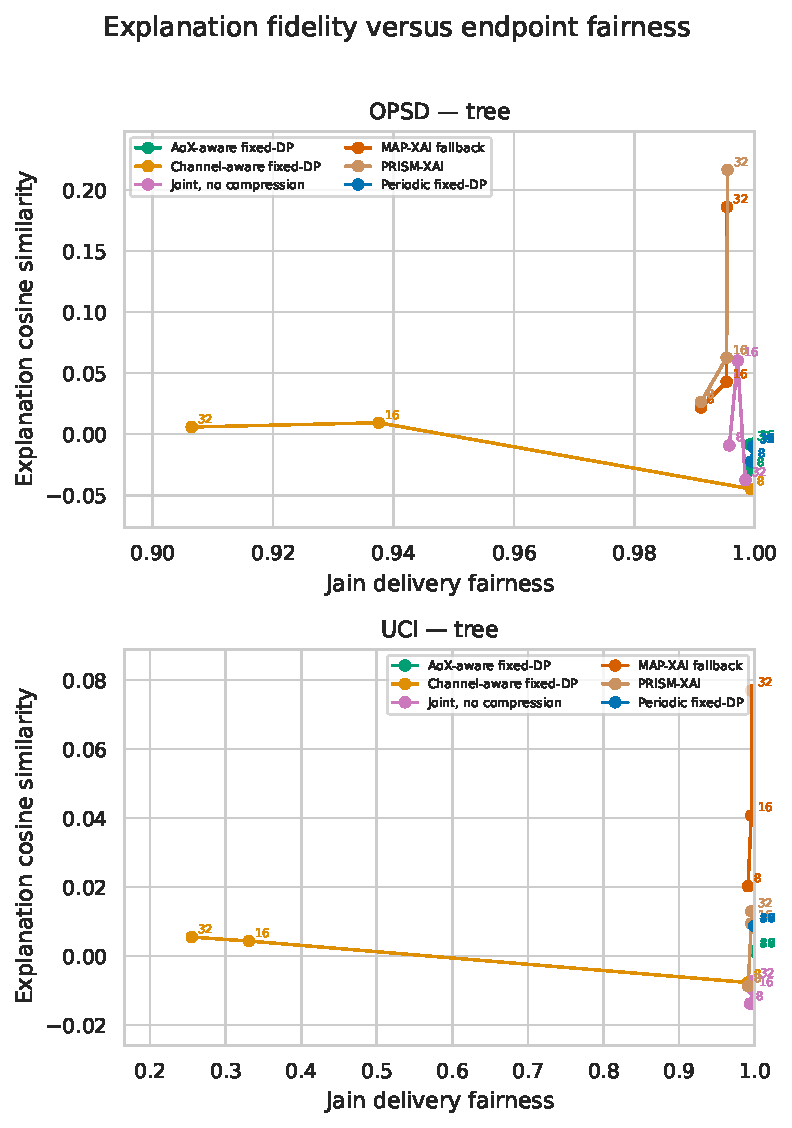
\includegraphics[width=.96\textwidth,height=.82\textheight,keepaspectratio]{../../SERVICE_TRADEOFF_RESULTS/runs/thr_2_cap_16/fairness_reliability.pdf}

\caption{Public-score threshold $\tau=2$, release cap $M=16$, Combined datasets: fairness--reliability plane. This panel should be read with the setting-level quantitative interpretation and the complete tables immediately preceding the figure block.}

\end{figure*}

\clearpage

\begin{figure*}[p]

\centering

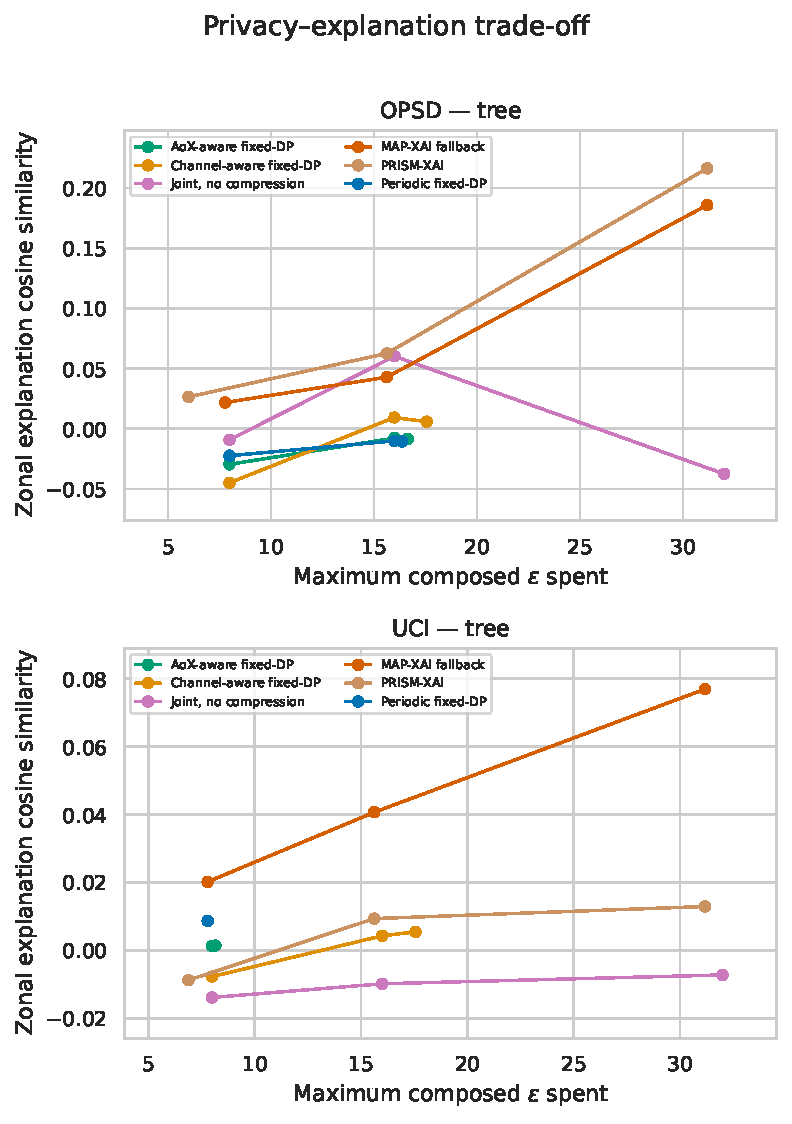
\includegraphics[width=.96\textwidth,height=.82\textheight,keepaspectratio]{../../SERVICE_TRADEOFF_RESULTS/runs/thr_2_cap_16/privacy_fidelity.pdf}

\caption{Public-score threshold $\tau=2$, release cap $M=16$, Combined datasets: privacy--fidelity plane. This panel should be read with the setting-level quantitative interpretation and the complete tables immediately preceding the figure block.}

\end{figure*}

\clearpage

\begin{figure*}[p]

\centering

\includegraphics[width=.96\textwidth,height=.82\textheight,keepaspectratio]{../../SERVICE_TRADEOFF_RESULTS/runs/thr_2_cap_16/pareto_bits_fidelity.pdf}

\caption{Public-score threshold $\tau=2$, release cap $M=16$, Combined datasets: traffic--fidelity Pareto plane. This panel should be read with the setting-level quantitative interpretation and the complete tables immediately preceding the figure block.}

\end{figure*}

\clearpage

\begin{figure*}[p]

\centering

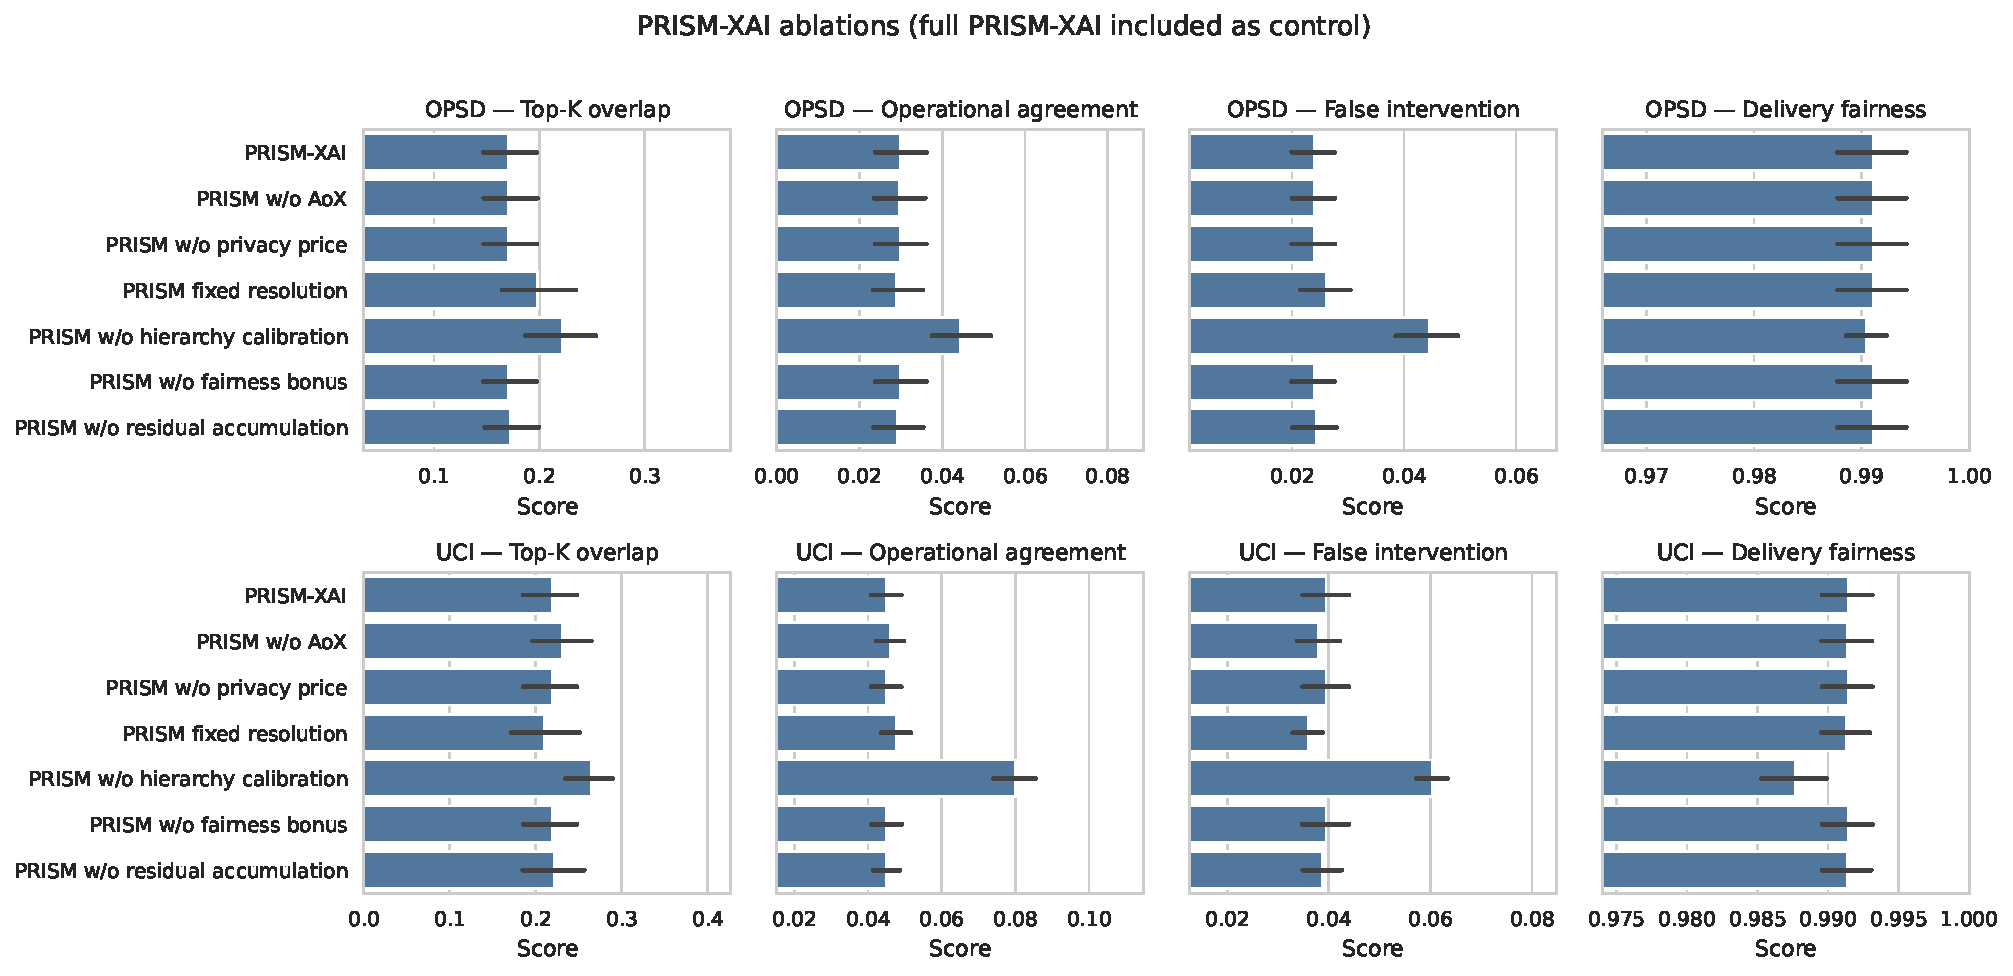
\includegraphics[width=.96\textwidth,height=.82\textheight,keepaspectratio]{../../SERVICE_TRADEOFF_RESULTS/runs/thr_2_cap_16/ablation_results.pdf}

\caption{Public-score threshold $\tau=2$, release cap $M=16$, Combined datasets: component ablation. This panel should be read with the setting-level quantitative interpretation and the complete tables immediately preceding the figure block.}

\end{figure*}

\clearpage

\paragraph{OPSD.} The three generated tables below report the full method means, all condition-level values, and paired differences. The five figures that follow provide the corresponding temporal, fairness, privacy, Pareto, and ablation views. Aggregate panels support the setting-level summary above; dataset panels reveal whether that summary is shared by OPSD and UCI rather than being driven by their different endpoint counts.

\begin{table*}[p]\centering\tiny

\caption{Public-score threshold $\tau=2$, release cap $M=16$, OPSD: complete generated method table.}

\label{tab:thr_2_cap_16:opsd:main}

\resizebox{\linewidth}{!}{% Values are means with 95% Student-t confidence intervals across seeds.
\begin{tabular}{lccccccccccccccc}
\toprule
Dataset & Model & $\epsilon_{\max}$ & Method & Top-$K$ & Cosine & Decision & Recall & Prec. & Abst. & P95 ms & kbit & Spent $\epsilon$ & False int. & bit/correct & Fairness \\
\midrule
OPSD & Tree & 8 & AoX-aware fixed-DP & 0.234 $\pm$ 0.048 & -0.033 $\pm$ 0.028 & 0.119 $\pm$ 0.028 & 0.119 $\pm$ 0.028 & 0.198 $\pm$ 0.054 & 0.721 $\pm$ 0.005 & 6.903 $\pm$ 1.126 & 1560.564 $\pm$ 0.000 & 7.990 $\pm$ 0.000 & 0.183 $\pm$ 0.020 & 35567.482 $\pm$ 10569.818 & 0.999 $\pm$ 0.000 \\
OPSD & Tree & 8 & AoX-aware fixed-DP & 0.238 $\pm$ 0.049 & -0.026 $\pm$ 0.055 & 0.121 $\pm$ 0.026 & 0.121 $\pm$ 0.026 & 0.205 $\pm$ 0.053 & 0.721 $\pm$ 0.005 & 6.903 $\pm$ 1.126 & 1560.564 $\pm$ 0.000 & 7.990 $\pm$ 0.000 & 0.179 $\pm$ 0.023 & 34123.214 $\pm$ 8376.542 & 0.999 $\pm$ 0.000 \\
OPSD & Tree & 8 & Channel-aware fixed-DP & 0.292 $\pm$ 0.037 & -0.041 $\pm$ 0.051 & 0.107 $\pm$ 0.026 & 0.107 $\pm$ 0.026 & 0.217 $\pm$ 0.068 & 0.779 $\pm$ 0.011 & 5.571 $\pm$ 1.784 & 1560.564 $\pm$ 0.000 & 7.990 $\pm$ 0.000 & 0.154 $\pm$ 0.029 & 40860.756 $\pm$ 14126.920 & 0.999 $\pm$ 0.000 \\
OPSD & Tree & 8 & Channel-aware fixed-DP & 0.292 $\pm$ 0.054 & -0.049 $\pm$ 0.064 & 0.111 $\pm$ 0.023 & 0.111 $\pm$ 0.023 & 0.228 $\pm$ 0.066 & 0.779 $\pm$ 0.011 & 5.571 $\pm$ 1.784 & 1560.564 $\pm$ 0.000 & 7.990 $\pm$ 0.000 & 0.149 $\pm$ 0.026 & 37980.855 $\pm$ 12338.094 & 0.999 $\pm$ 0.000 \\
OPSD & Tree & 8 & Joint, no compression & 0.288 $\pm$ 0.064 & -0.030 $\pm$ 0.079 & 0.016 $\pm$ 0.005 & 0.016 $\pm$ 0.005 & 0.193 $\pm$ 0.059 & 0.957 $\pm$ 0.003 & 4.560 $\pm$ 1.811 & 189.900 $\pm$ 0.554 & 7.990 $\pm$ 0.000 & 0.027 $\pm$ 0.005 & 32490.357 $\pm$ 10149.755 & 0.996 $\pm$ 0.002 \\
OPSD & Tree & 8 & Joint, no compression & 0.258 $\pm$ 0.055 & 0.011 $\pm$ 0.094 & 0.019 $\pm$ 0.004 & 0.019 $\pm$ 0.004 & 0.224 $\pm$ 0.044 & 0.957 $\pm$ 0.003 & 4.562 $\pm$ 1.809 & 189.750 $\pm$ 0.566 & 7.990 $\pm$ 0.000 & 0.025 $\pm$ 0.003 & 26079.167 $\pm$ 6335.386 & 0.996 $\pm$ 0.002 \\
OPSD & Tree & 8 & Periodic fixed-DP & 0.241 $\pm$ 0.049 & -0.019 $\pm$ 0.061 & 0.125 $\pm$ 0.020 & 0.125 $\pm$ 0.020 & 0.209 $\pm$ 0.044 & 0.722 $\pm$ 0.006 & 6.303 $\pm$ 1.438 & 1560.564 $\pm$ 0.000 & 7.990 $\pm$ 0.000 & 0.181 $\pm$ 0.021 & 31183.082 $\pm$ 4356.378 & 0.999 $\pm$ 0.000 \\
OPSD & Tree & 8 & Periodic fixed-DP & 0.242 $\pm$ 0.048 & -0.026 $\pm$ 0.082 & 0.135 $\pm$ 0.016 & 0.135 $\pm$ 0.016 & 0.231 $\pm$ 0.037 & 0.722 $\pm$ 0.006 & 6.303 $\pm$ 1.438 & 1560.564 $\pm$ 0.000 & 7.990 $\pm$ 0.000 & 0.169 $\pm$ 0.017 & 28520.235 $\pm$ 3511.595 & 0.999 $\pm$ 0.000 \\
OPSD & Tree & 8 & PRISM-XAI & 0.170 $\pm$ 0.039 & 0.027 $\pm$ 0.072 & 0.029 $\pm$ 0.012 & 0.029 $\pm$ 0.012 & 0.326 $\pm$ 0.147 & 0.938 $\pm$ 0.004 & 4.881 $\pm$ 1.730 & 88.137 $\pm$ 0.577 & 6.066 $\pm$ 0.239 & 0.024 $\pm$ 0.007 & 10754.619 $\pm$ 5615.749 & 0.991 $\pm$ 0.006 \\
OPSD & Tree & 8 & PRISM-XAI & 0.171 $\pm$ 0.046 & 0.026 $\pm$ 0.082 & 0.031 $\pm$ 0.010 & 0.031 $\pm$ 0.010 & 0.343 $\pm$ 0.130 & 0.938 $\pm$ 0.004 & 4.873 $\pm$ 1.737 & 87.707 $\pm$ 0.532 & 5.936 $\pm$ 0.213 & 0.024 $\pm$ 0.007 & 8388.650 $\pm$ 2960.712 & 0.991 $\pm$ 0.006 \\
OPSD & Tree & 8 & MAP-XAI fallback & 0.203 $\pm$ 0.058 & 0.019 $\pm$ 0.075 & 0.029 $\pm$ 0.011 & 0.029 $\pm$ 0.011 & 0.324 $\pm$ 0.148 & 0.938 $\pm$ 0.004 & 4.960 $\pm$ 1.678 & 105.889 $\pm$ 0.169 & 7.786 $\pm$ 0.000 & 0.026 $\pm$ 0.008 & 11344.761 $\pm$ 4319.900 & 0.991 $\pm$ 0.006 \\
OPSD & Tree & 8 & MAP-XAI fallback & 0.181 $\pm$ 0.054 & 0.025 $\pm$ 0.081 & 0.029 $\pm$ 0.009 & 0.029 $\pm$ 0.009 & 0.310 $\pm$ 0.118 & 0.938 $\pm$ 0.004 & 4.960 $\pm$ 1.678 & 105.737 $\pm$ 0.152 & 7.786 $\pm$ 0.000 & 0.026 $\pm$ 0.007 & 10402.432 $\pm$ 2994.804 & 0.991 $\pm$ 0.006 \\
\bottomrule
\end{tabular}
}

\end{table*}\clearpage

\begin{table*}[p]\centering\tiny

\caption{Public-score threshold $\tau=2$, release cap $M=16$, OPSD: complete condition-level generated table.}

\label{tab:thr_2_cap_16:opsd:conditions}

\resizebox{\textwidth}{!}{\begin{tabular}{llllccccccccccc}
\toprule
Dataset & Model & $\epsilon_{\max}$ & Method & kbit & Top-$K$ & Random Top-$K$ & Cosine & Decision & Recall & Precision & Coverage & Abstain & False int. & Spent $\epsilon$ \\
\midrule
OPSD & Tree & 8 & Joint, no compression & 189.900 $\pm$ 0.554 & 0.288 $\pm$ 0.064 & 0.250 $\pm$ 0.000 & -0.030 $\pm$ 0.079 & 0.016 $\pm$ 0.005 & 0.016 $\pm$ 0.005 & 0.193 $\pm$ 0.059 & 0.043 $\pm$ 0.003 & 0.957 $\pm$ 0.003 & 0.027 $\pm$ 0.005 & 7.990 $\pm$ 0.000 \\
OPSD & Tree & 8 & Joint, no compression & 189.750 $\pm$ 0.566 & 0.258 $\pm$ 0.055 & 0.250 $\pm$ 0.000 & 0.011 $\pm$ 0.094 & 0.019 $\pm$ 0.004 & 0.019 $\pm$ 0.004 & 0.224 $\pm$ 0.044 & 0.043 $\pm$ 0.003 & 0.957 $\pm$ 0.003 & 0.025 $\pm$ 0.003 & 7.990 $\pm$ 0.000 \\
OPSD & Tree & 8 & Periodic fixed-DP & 1560.564 $\pm$ 0.000 & 0.241 $\pm$ 0.049 & 0.250 $\pm$ 0.000 & -0.019 $\pm$ 0.061 & 0.125 $\pm$ 0.020 & 0.125 $\pm$ 0.020 & 0.209 $\pm$ 0.044 & 0.278 $\pm$ 0.006 & 0.722 $\pm$ 0.006 & 0.181 $\pm$ 0.021 & 7.990 $\pm$ 0.000 \\
OPSD & Tree & 8 & Periodic fixed-DP & 1560.564 $\pm$ 0.000 & 0.242 $\pm$ 0.048 & 0.250 $\pm$ 0.000 & -0.026 $\pm$ 0.082 & 0.135 $\pm$ 0.016 & 0.135 $\pm$ 0.016 & 0.231 $\pm$ 0.037 & 0.278 $\pm$ 0.006 & 0.722 $\pm$ 0.006 & 0.169 $\pm$ 0.017 & 7.990 $\pm$ 0.000 \\
OPSD & Tree & 8 & PRISM-XAI & 88.137 $\pm$ 0.577 & 0.170 $\pm$ 0.039 & 0.250 $\pm$ 0.000 & 0.027 $\pm$ 0.072 & 0.029 $\pm$ 0.012 & 0.029 $\pm$ 0.012 & 0.326 $\pm$ 0.147 & 0.062 $\pm$ 0.004 & 0.938 $\pm$ 0.004 & 0.024 $\pm$ 0.007 & 6.066 $\pm$ 0.239 \\
OPSD & Tree & 8 & PRISM-XAI & 87.707 $\pm$ 0.532 & 0.171 $\pm$ 0.046 & 0.250 $\pm$ 0.000 & 0.026 $\pm$ 0.082 & 0.031 $\pm$ 0.010 & 0.031 $\pm$ 0.010 & 0.343 $\pm$ 0.130 & 0.062 $\pm$ 0.004 & 0.938 $\pm$ 0.004 & 0.024 $\pm$ 0.007 & 5.936 $\pm$ 0.213 \\
OPSD & Tree & 16 & Joint, no compression & 459.900 $\pm$ 0.750 & 0.232 $\pm$ 0.065 & 0.250 $\pm$ 0.000 & 0.059 $\pm$ 0.048 & 0.038 $\pm$ 0.009 & 0.038 $\pm$ 0.009 & 0.222 $\pm$ 0.049 & 0.088 $\pm$ 0.004 & 0.912 $\pm$ 0.004 & 0.049 $\pm$ 0.005 & 15.997 $\pm$ 0.000 \\
OPSD & Tree & 16 & Joint, no compression & 460.050 $\pm$ 0.724 & 0.241 $\pm$ 0.055 & 0.250 $\pm$ 0.000 & 0.061 $\pm$ 0.052 & 0.039 $\pm$ 0.008 & 0.039 $\pm$ 0.008 & 0.241 $\pm$ 0.042 & 0.088 $\pm$ 0.004 & 0.912 $\pm$ 0.004 & 0.045 $\pm$ 0.004 & 15.997 $\pm$ 0.000 \\
OPSD & Tree & 16 & Periodic fixed-DP & 5112.594 $\pm$ 0.000 & 0.249 $\pm$ 0.022 & 0.250 $\pm$ 0.000 & -0.009 $\pm$ 0.045 & 0.450 $\pm$ 0.062 & 0.450 $\pm$ 0.062 & 0.237 $\pm$ 0.042 & 0.985 $\pm$ 0.002 & 0.015 $\pm$ 0.002 & 0.551 $\pm$ 0.057 & 15.997 $\pm$ 0.000 \\
OPSD & Tree & 16 & Periodic fixed-DP & 5112.594 $\pm$ 0.000 & 0.243 $\pm$ 0.019 & 0.250 $\pm$ 0.000 & -0.012 $\pm$ 0.050 & 0.463 $\pm$ 0.047 & 0.463 $\pm$ 0.047 & 0.240 $\pm$ 0.028 & 0.985 $\pm$ 0.002 & 0.015 $\pm$ 0.002 & 0.547 $\pm$ 0.036 & 15.997 $\pm$ 0.000 \\
OPSD & Tree & 16 & PRISM-XAI & 176.428 $\pm$ 0.771 & 0.259 $\pm$ 0.050 & 0.250 $\pm$ 0.000 & 0.054 $\pm$ 0.064 & 0.053 $\pm$ 0.015 & 0.053 $\pm$ 0.015 & 0.339 $\pm$ 0.133 & 0.120 $\pm$ 0.006 & 0.880 $\pm$ 0.006 & 0.042 $\pm$ 0.011 & 15.620 $\pm$ 0.000 \\
OPSD & Tree & 16 & PRISM-XAI & 175.629 $\pm$ 0.704 & 0.256 $\pm$ 0.054 & 0.250 $\pm$ 0.000 & 0.071 $\pm$ 0.073 & 0.050 $\pm$ 0.013 & 0.050 $\pm$ 0.013 & 0.291 $\pm$ 0.104 & 0.120 $\pm$ 0.006 & 0.880 $\pm$ 0.006 & 0.049 $\pm$ 0.010 & 15.620 $\pm$ 0.000 \\
OPSD & Tree & 32 & Joint, no compression & 1140.900 $\pm$ 7.953 & 0.235 $\pm$ 0.064 & 0.250 $\pm$ 0.000 & -0.031 $\pm$ 0.089 & 0.074 $\pm$ 0.015 & 0.074 $\pm$ 0.015 & 0.205 $\pm$ 0.039 & 0.157 $\pm$ 0.006 & 0.843 $\pm$ 0.006 & 0.107 $\pm$ 0.009 & 31.999 $\pm$ 0.000 \\
OPSD & Tree & 32 & Joint, no compression & 1140.900 $\pm$ 7.953 & 0.282 $\pm$ 0.054 & 0.250 $\pm$ 0.000 & -0.044 $\pm$ 0.076 & 0.080 $\pm$ 0.011 & 0.080 $\pm$ 0.011 & 0.227 $\pm$ 0.052 & 0.158 $\pm$ 0.006 & 0.842 $\pm$ 0.006 & 0.105 $\pm$ 0.015 & 31.999 $\pm$ 0.000 \\
OPSD & Tree & 32 & Periodic fixed-DP & 5299.836 $\pm$ 0.625 & 0.249 $\pm$ 0.022 & 0.250 $\pm$ 0.000 & -0.009 $\pm$ 0.044 & 0.458 $\pm$ 0.066 & 0.458 $\pm$ 0.066 & 0.237 $\pm$ 0.045 & 1.000 $\pm$ 0.000 & 0.000 $\pm$ 0.000 & 0.562 $\pm$ 0.062 & 16.371 $\pm$ 0.000 \\
OPSD & Tree & 32 & Periodic fixed-DP & 5299.836 $\pm$ 0.625 & 0.244 $\pm$ 0.019 & 0.250 $\pm$ 0.000 & -0.012 $\pm$ 0.050 & 0.471 $\pm$ 0.049 & 0.471 $\pm$ 0.049 & 0.240 $\pm$ 0.029 & 1.000 $\pm$ 0.000 & 0.000 $\pm$ 0.000 & 0.559 $\pm$ 0.039 & 16.371 $\pm$ 0.000 \\
OPSD & Tree & 32 & PRISM-XAI & 176.336 $\pm$ 0.759 & 0.315 $\pm$ 0.088 & 0.250 $\pm$ 0.000 & 0.193 $\pm$ 0.062 & 0.061 $\pm$ 0.013 & 0.061 $\pm$ 0.013 & 0.397 $\pm$ 0.114 & 0.120 $\pm$ 0.006 & 0.880 $\pm$ 0.006 & 0.037 $\pm$ 0.010 & 31.175 $\pm$ 0.000 \\
OPSD & Tree & 32 & PRISM-XAI & 175.415 $\pm$ 0.593 & 0.314 $\pm$ 0.062 & 0.250 $\pm$ 0.000 & 0.240 $\pm$ 0.062 & 0.060 $\pm$ 0.013 & 0.060 $\pm$ 0.013 & 0.365 $\pm$ 0.089 & 0.120 $\pm$ 0.006 & 0.880 $\pm$ 0.006 & 0.040 $\pm$ 0.008 & 31.175 $\pm$ 0.000 \\
\bottomrule
\end{tabular}
}

\end{table*}\clearpage

\begin{table*}[p]\centering\tiny

\caption{Public-score threshold $\tau=2$, release cap $M=16$, OPSD: complete generated paired comparisons.}

\label{tab:thr_2_cap_16:opsd:paired}

\resizebox{\textwidth}{!}{\begin{tabular}{llcccc}
\toprule
Dataset & Baseline & Delta kbit & Delta Top-$K$ & Delta recall & Delta fairness \\
\midrule
OPSD & AoX-aware fixed-DP & -1472.427 $\pm$ 0.577 & -0.064 $\pm$ 0.057 & -0.091 $\pm$ 0.033 & -0.008 $\pm$ 0.006 \\
OPSD & AoX-aware fixed-DP & -4923.485 $\pm$ 5.595 & 0.006 $\pm$ 0.053 & -0.349 $\pm$ 0.082 & -0.004 $\pm$ 0.002 \\
OPSD & AoX-aware fixed-DP & -5123.888 $\pm$ 0.759 & 0.062 $\pm$ 0.093 & -0.351 $\pm$ 0.083 & -0.004 $\pm$ 0.002 \\
OPSD & AoX-aware fixed-DP & -1472.857 $\pm$ 0.532 & -0.068 $\pm$ 0.063 & -0.090 $\pm$ 0.028 & -0.008 $\pm$ 0.006 \\
OPSD & AoX-aware fixed-DP & -4924.283 $\pm$ 5.582 & 0.004 $\pm$ 0.062 & -0.364 $\pm$ 0.062 & -0.004 $\pm$ 0.002 \\
OPSD & AoX-aware fixed-DP & -5124.809 $\pm$ 0.593 & 0.062 $\pm$ 0.071 & -0.366 $\pm$ 0.060 & -0.004 $\pm$ 0.002 \\
OPSD & Channel-aware fixed-DP & -1472.427 $\pm$ 0.577 & -0.122 $\pm$ 0.049 & -0.078 $\pm$ 0.029 & -0.008 $\pm$ 0.006 \\
OPSD & Channel-aware fixed-DP & -4510.181 $\pm$ 12.999 & -0.002 $\pm$ 0.048 & -0.349 $\pm$ 0.095 & 0.058 $\pm$ 0.005 \\
OPSD & Channel-aware fixed-DP & -5123.888 $\pm$ 0.759 & 0.057 $\pm$ 0.093 & -0.373 $\pm$ 0.102 & 0.089 $\pm$ 0.006 \\
OPSD & Channel-aware fixed-DP & -1472.857 $\pm$ 0.532 & -0.122 $\pm$ 0.074 & -0.080 $\pm$ 0.025 & -0.008 $\pm$ 0.006 \\
OPSD & Channel-aware fixed-DP & -4510.980 $\pm$ 13.099 & -0.002 $\pm$ 0.051 & -0.369 $\pm$ 0.093 & 0.058 $\pm$ 0.005 \\
OPSD & Channel-aware fixed-DP & -5124.809 $\pm$ 0.593 & 0.057 $\pm$ 0.070 & -0.396 $\pm$ 0.090 & 0.089 $\pm$ 0.006 \\
OPSD & Joint, no compression & -101.763 $\pm$ 0.687 & -0.118 $\pm$ 0.078 & 0.012 $\pm$ 0.011 & -0.005 $\pm$ 0.005 \\
OPSD & Joint, no compression & -283.472 $\pm$ 1.424 & 0.028 $\pm$ 0.096 & 0.015 $\pm$ 0.017 & -0.002 $\pm$ 0.002 \\
OPSD & Joint, no compression & -964.564 $\pm$ 8.170 & 0.080 $\pm$ 0.106 & -0.013 $\pm$ 0.022 & -0.003 $\pm$ 0.002 \\
OPSD & Joint, no compression & -102.043 $\pm$ 0.513 & -0.088 $\pm$ 0.080 & 0.012 $\pm$ 0.009 & -0.005 $\pm$ 0.005 \\
OPSD & Joint, no compression & -284.421 $\pm$ 1.294 & 0.015 $\pm$ 0.063 & 0.011 $\pm$ 0.014 & -0.002 $\pm$ 0.002 \\
OPSD & Joint, no compression & -965.485 $\pm$ 8.153 & 0.032 $\pm$ 0.101 & -0.020 $\pm$ 0.016 & -0.003 $\pm$ 0.002 \\
OPSD & Periodic fixed-DP & -1472.427 $\pm$ 0.577 & -0.070 $\pm$ 0.050 & -0.096 $\pm$ 0.024 & -0.008 $\pm$ 0.006 \\
OPSD & Periodic fixed-DP & -4936.166 $\pm$ 0.771 & 0.010 $\pm$ 0.060 & -0.398 $\pm$ 0.067 & -0.004 $\pm$ 0.002 \\
OPSD & Periodic fixed-DP & -5123.500 $\pm$ 0.672 & 0.066 $\pm$ 0.097 & -0.397 $\pm$ 0.070 & -0.004 $\pm$ 0.002 \\
OPSD & Periodic fixed-DP & -1472.857 $\pm$ 0.532 & -0.071 $\pm$ 0.050 & -0.104 $\pm$ 0.018 & -0.008 $\pm$ 0.006 \\
OPSD & Periodic fixed-DP & -4936.965 $\pm$ 0.704 & 0.013 $\pm$ 0.062 & -0.412 $\pm$ 0.051 & -0.004 $\pm$ 0.002 \\
OPSD & Periodic fixed-DP & -5124.421 $\pm$ 0.602 & 0.070 $\pm$ 0.071 & -0.411 $\pm$ 0.048 & -0.004 $\pm$ 0.002 \\
OPSD & MAP-XAI fallback & -17.751 $\pm$ 0.664 & -0.033 $\pm$ 0.057 & -0.000 $\pm$ 0.007 & 0.000 $\pm$ 0.000 \\
OPSD & MAP-XAI fallback & -37.461 $\pm$ 0.817 & 0.030 $\pm$ 0.036 & 0.009 $\pm$ 0.010 & 0.000 $\pm$ 0.000 \\
OPSD & MAP-XAI fallback & -37.553 $\pm$ 0.814 & 0.025 $\pm$ 0.073 & 0.005 $\pm$ 0.009 & 0.000 $\pm$ 0.000 \\
OPSD & MAP-XAI fallback & -18.030 $\pm$ 0.589 & -0.010 $\pm$ 0.051 & 0.002 $\pm$ 0.006 & 0.000 $\pm$ 0.000 \\
OPSD & MAP-XAI fallback & -38.108 $\pm$ 0.765 & 0.032 $\pm$ 0.027 & 0.007 $\pm$ 0.006 & 0.000 $\pm$ 0.000 \\
OPSD & MAP-XAI fallback & -38.323 $\pm$ 0.668 & 0.046 $\pm$ 0.040 & 0.003 $\pm$ 0.008 & 0.000 $\pm$ 0.000 \\
\bottomrule
\end{tabular}
}

\end{table*}\clearpage

\begin{figure*}[p]

\centering

\includegraphics[width=.96\textwidth,height=.82\textheight,keepaspectratio]{../../SERVICE_TRADEOFF_RESULTS/runs/thr_2_cap_16/opsd/regime_trace.pdf}

\caption{Public-score threshold $\tau=2$, release cap $M=16$, OPSD: representative regime trace. This panel should be read with the setting-level quantitative interpretation and the complete tables immediately preceding the figure block.}

\end{figure*}

\clearpage

\begin{figure*}[p]

\centering

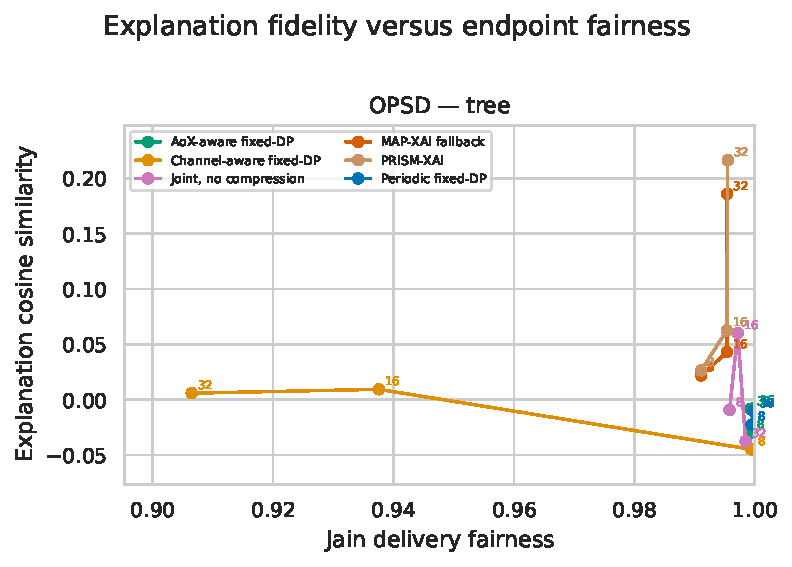
\includegraphics[width=.96\textwidth,height=.82\textheight,keepaspectratio]{../../SERVICE_TRADEOFF_RESULTS/runs/thr_2_cap_16/opsd/fairness_reliability.pdf}

\caption{Public-score threshold $\tau=2$, release cap $M=16$, OPSD: fairness--reliability plane. This panel should be read with the setting-level quantitative interpretation and the complete tables immediately preceding the figure block.}

\end{figure*}

\clearpage

\begin{figure*}[p]

\centering

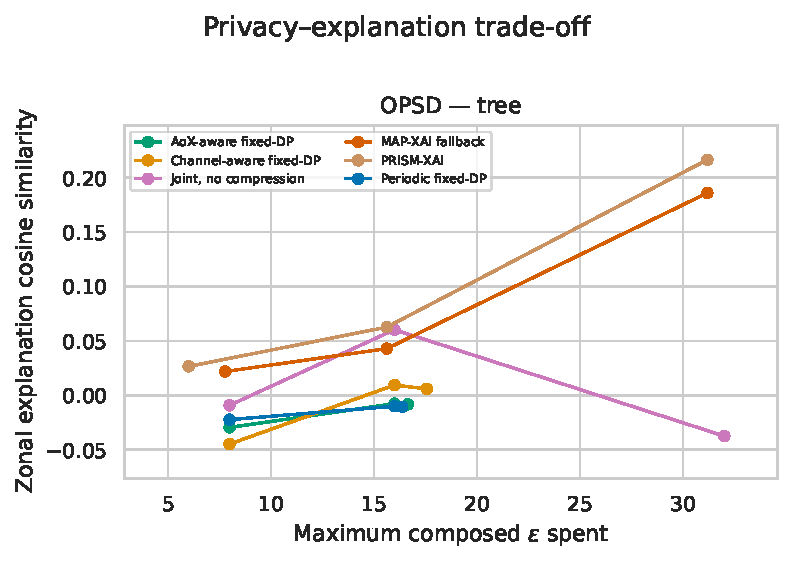
\includegraphics[width=.96\textwidth,height=.82\textheight,keepaspectratio]{../../SERVICE_TRADEOFF_RESULTS/runs/thr_2_cap_16/opsd/privacy_fidelity.pdf}

\caption{Public-score threshold $\tau=2$, release cap $M=16$, OPSD: privacy--fidelity plane. This panel should be read with the setting-level quantitative interpretation and the complete tables immediately preceding the figure block.}

\end{figure*}

\clearpage

\begin{figure*}[p]

\centering

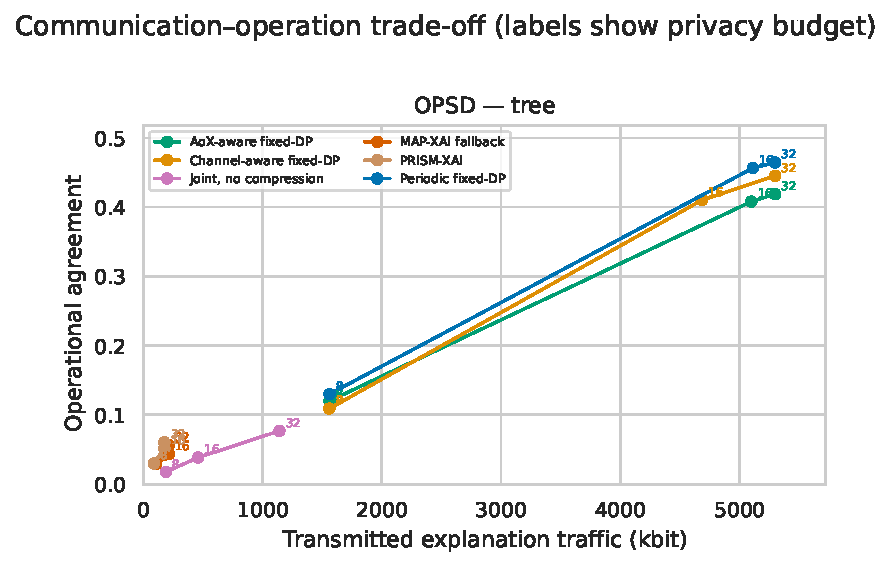
\includegraphics[width=.96\textwidth,height=.82\textheight,keepaspectratio]{../../SERVICE_TRADEOFF_RESULTS/runs/thr_2_cap_16/opsd/pareto_bits_fidelity.pdf}

\caption{Public-score threshold $\tau=2$, release cap $M=16$, OPSD: traffic--fidelity Pareto plane. This panel should be read with the setting-level quantitative interpretation and the complete tables immediately preceding the figure block.}

\end{figure*}

\clearpage

\begin{figure*}[p]

\centering

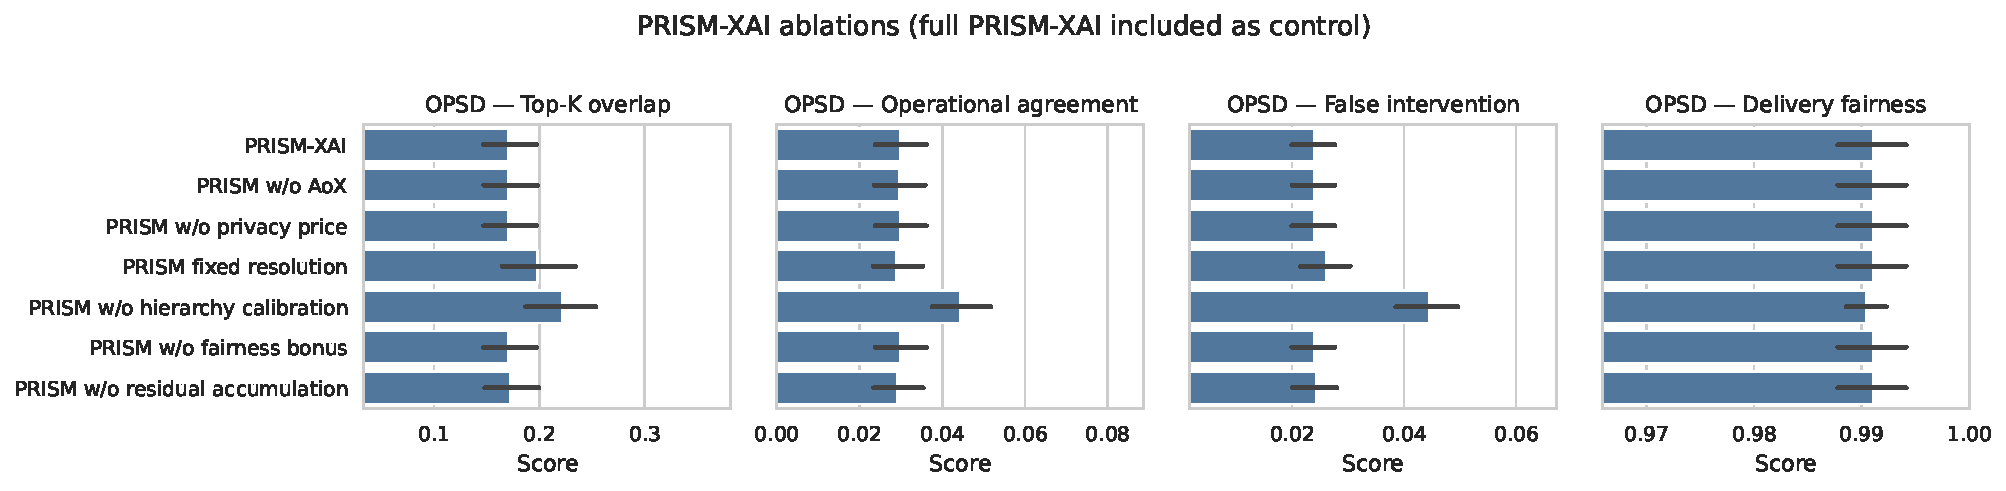
\includegraphics[width=.96\textwidth,height=.82\textheight,keepaspectratio]{../../SERVICE_TRADEOFF_RESULTS/runs/thr_2_cap_16/opsd/ablation_results.pdf}

\caption{Public-score threshold $\tau=2$, release cap $M=16$, OPSD: component ablation. This panel should be read with the setting-level quantitative interpretation and the complete tables immediately preceding the figure block.}

\end{figure*}

\clearpage

\paragraph{UCI.} The three generated tables below report the full method means, all condition-level values, and paired differences. The five figures that follow provide the corresponding temporal, fairness, privacy, Pareto, and ablation views. Aggregate panels support the setting-level summary above; dataset panels reveal whether that summary is shared by OPSD and UCI rather than being driven by their different endpoint counts.

\begin{table*}[p]\centering\tiny

\caption{Public-score threshold $\tau=2$, release cap $M=16$, UCI: complete generated method table.}

\label{tab:thr_2_cap_16:uci:main}

\resizebox{\linewidth}{!}{% Values are means with 95% Student-t confidence intervals across seeds.
\begin{tabular}{lccccccccccccccc}
\toprule
Dataset & Model & $\epsilon_{\max}$ & Method & Top-$K$ & Cosine & Decision & Recall & Prec. & Abst. & P95 ms & kbit & Spent $\epsilon$ & False int. & bit/correct & Fairness \\
\midrule
UCI & Tree & 8 & AoX-aware fixed-DP & 0.263 $\pm$ 0.041 & -0.007 $\pm$ 0.009 & 0.457 $\pm$ 0.031 & 0.457 $\pm$ 0.031 & 0.362 $\pm$ 0.024 & 0.003 $\pm$ 0.001 & 7.500 $\pm$ 0.000 & 5300.224 $\pm$ 0.000 & 7.990 $\pm$ 0.000 & 0.557 $\pm$ 0.025 & 14002.896 $\pm$ 1040.243 & 0.999 $\pm$ 0.000 \\
UCI & Tree & 8 & AoX-aware fixed-DP & 0.260 $\pm$ 0.022 & 0.010 $\pm$ 0.055 & 0.455 $\pm$ 0.047 & 0.455 $\pm$ 0.047 & 0.361 $\pm$ 0.038 & 0.003 $\pm$ 0.001 & 7.500 $\pm$ 0.000 & 5300.224 $\pm$ 0.000 & 7.990 $\pm$ 0.000 & 0.557 $\pm$ 0.048 & 14198.303 $\pm$ 1508.274 & 0.999 $\pm$ 0.000 \\
UCI & Tree & 8 & Channel-aware fixed-DP & 0.248 $\pm$ 0.031 & 0.004 $\pm$ 0.012 & 0.001 $\pm$ 0.001 & 0.001 $\pm$ 0.001 & 0.150 $\pm$ 0.151 & 0.999 $\pm$ 0.001 & 4.609 $\pm$ 1.781 & 5295.177 $\pm$ 3.740 & 7.990 $\pm$ 0.000 & 0.001 $\pm$ 0.001 & 4632196.500 $\pm$ 2102650.252 & 0.991 $\pm$ 0.001 \\
UCI & Tree & 8 & Channel-aware fixed-DP & 0.239 $\pm$ 0.030 & -0.020 $\pm$ 0.055 & 0.000 $\pm$ 0.000 & 0.000 $\pm$ 0.000 & 0.117 $\pm$ 0.225 & 0.999 $\pm$ 0.001 & 4.609 $\pm$ 1.781 & 5295.177 $\pm$ 3.740 & 7.990 $\pm$ 0.000 & 0.001 $\pm$ 0.001 & 5296989.000 $\pm$ 41104.572 & 0.991 $\pm$ 0.001 \\
UCI & Tree & 8 & Joint, no compression & 0.286 $\pm$ 0.045 & 0.004 $\pm$ 0.020 & 0.052 $\pm$ 0.005 & 0.052 $\pm$ 0.005 & 0.406 $\pm$ 0.037 & 0.875 $\pm$ 0.003 & 5.123 $\pm$ 1.792 & 672.300 $\pm$ 0.452 & 7.990 $\pm$ 0.000 & 0.053 $\pm$ 0.004 & 15676.175 $\pm$ 1475.621 & 0.994 $\pm$ 0.003 \\
UCI & Tree & 8 & Joint, no compression & 0.229 $\pm$ 0.052 & -0.032 $\pm$ 0.050 & 0.057 $\pm$ 0.007 & 0.057 $\pm$ 0.007 & 0.428 $\pm$ 0.041 & 0.875 $\pm$ 0.003 & 5.131 $\pm$ 1.787 & 672.300 $\pm$ 0.452 & 7.990 $\pm$ 0.000 & 0.052 $\pm$ 0.004 & 14702.786 $\pm$ 2334.488 & 0.994 $\pm$ 0.003 \\
UCI & Tree & 8 & Periodic fixed-DP & 0.259 $\pm$ 0.060 & -0.005 $\pm$ 0.008 & 0.006 $\pm$ 0.001 & 0.006 $\pm$ 0.001 & 0.244 $\pm$ 0.049 & 0.989 $\pm$ 0.001 & 4.596 $\pm$ 1.788 & 5299.318 $\pm$ 1.451 & 7.786 $\pm$ 0.000 & 0.013 $\pm$ 0.002 & 1215103.896 $\pm$ 390671.319 & 0.999 $\pm$ 0.000 \\
UCI & Tree & 8 & Periodic fixed-DP & 0.260 $\pm$ 0.044 & 0.022 $\pm$ 0.070 & 0.005 $\pm$ 0.001 & 0.005 $\pm$ 0.001 & 0.195 $\pm$ 0.050 & 0.989 $\pm$ 0.001 & 4.596 $\pm$ 1.788 & 5299.318 $\pm$ 1.451 & 7.786 $\pm$ 0.000 & 0.015 $\pm$ 0.002 & 1555837.203 $\pm$ 955472.503 & 0.999 $\pm$ 0.000 \\
UCI & Tree & 8 & PRISM-XAI & 0.220 $\pm$ 0.061 & -0.009 $\pm$ 0.015 & 0.045 $\pm$ 0.006 & 0.045 $\pm$ 0.006 & 0.442 $\pm$ 0.072 & 0.906 $\pm$ 0.004 & 4.504 $\pm$ 1.537 & 325.842 $\pm$ 1.091 & 6.877 $\pm$ 0.090 & 0.040 $\pm$ 0.007 & 8917.519 $\pm$ 1309.048 & 0.992 $\pm$ 0.002 \\
UCI & Tree & 8 & PRISM-XAI & 0.217 $\pm$ 0.043 & -0.008 $\pm$ 0.077 & 0.045 $\pm$ 0.007 & 0.045 $\pm$ 0.007 & 0.447 $\pm$ 0.078 & 0.908 $\pm$ 0.002 & 5.058 $\pm$ 1.846 & 322.524 $\pm$ 0.793 & 6.877 $\pm$ 0.090 & 0.039 $\pm$ 0.008 & 9128.968 $\pm$ 1604.303 & 0.991 $\pm$ 0.004 \\
UCI & Tree & 8 & MAP-XAI fallback & 0.155 $\pm$ 0.082 & 0.000 $\pm$ 0.016 & 0.047 $\pm$ 0.007 & 0.047 $\pm$ 0.007 & 0.456 $\pm$ 0.051 & 0.905 $\pm$ 0.004 & 4.584 $\pm$ 1.508 & 381.745 $\pm$ 0.387 & 7.787 $\pm$ 0.001 & 0.038 $\pm$ 0.003 & 10122.948 $\pm$ 1695.832 & 0.992 $\pm$ 0.002 \\
UCI & Tree & 8 & MAP-XAI fallback & 0.221 $\pm$ 0.054 & 0.040 $\pm$ 0.080 & 0.046 $\pm$ 0.008 & 0.046 $\pm$ 0.008 & 0.469 $\pm$ 0.072 & 0.907 $\pm$ 0.003 & 4.763 $\pm$ 1.714 & 381.283 $\pm$ 0.251 & 7.787 $\pm$ 0.001 & 0.036 $\pm$ 0.006 & 10525.744 $\pm$ 1825.173 & 0.991 $\pm$ 0.004 \\
\bottomrule
\end{tabular}
}

\end{table*}\clearpage

\begin{table*}[p]\centering\tiny

\caption{Public-score threshold $\tau=2$, release cap $M=16$, UCI: complete condition-level generated table.}

\label{tab:thr_2_cap_16:uci:conditions}

\resizebox{\textwidth}{!}{\begin{tabular}{llllccccccccccc}
\toprule
Dataset & Model & $\epsilon_{\max}$ & Method & kbit & Top-$K$ & Random Top-$K$ & Cosine & Decision & Recall & Precision & Coverage & Abstain & False int. & Spent $\epsilon$ \\
\midrule
UCI & Tree & 8 & Joint, no compression & 672.300 $\pm$ 0.452 & 0.286 $\pm$ 0.045 & 0.250 $\pm$ 0.000 & 0.004 $\pm$ 0.020 & 0.052 $\pm$ 0.005 & 0.052 $\pm$ 0.005 & 0.406 $\pm$ 0.037 & 0.125 $\pm$ 0.003 & 0.875 $\pm$ 0.003 & 0.053 $\pm$ 0.004 & 7.990 $\pm$ 0.000 \\
UCI & Tree & 8 & Joint, no compression & 672.300 $\pm$ 0.452 & 0.229 $\pm$ 0.052 & 0.250 $\pm$ 0.000 & -0.032 $\pm$ 0.050 & 0.057 $\pm$ 0.007 & 0.057 $\pm$ 0.007 & 0.428 $\pm$ 0.041 & 0.125 $\pm$ 0.003 & 0.875 $\pm$ 0.003 & 0.052 $\pm$ 0.004 & 7.990 $\pm$ 0.000 \\
UCI & Tree & 8 & Periodic fixed-DP & 5299.318 $\pm$ 1.451 & 0.259 $\pm$ 0.060 & 0.250 $\pm$ 0.000 & -0.005 $\pm$ 0.008 & 0.006 $\pm$ 0.001 & 0.006 $\pm$ 0.001 & 0.244 $\pm$ 0.049 & 0.011 $\pm$ 0.001 & 0.989 $\pm$ 0.001 & 0.013 $\pm$ 0.002 & 7.786 $\pm$ 0.000 \\
UCI & Tree & 8 & Periodic fixed-DP & 5299.318 $\pm$ 1.451 & 0.260 $\pm$ 0.044 & 0.250 $\pm$ 0.000 & 0.022 $\pm$ 0.070 & 0.005 $\pm$ 0.001 & 0.005 $\pm$ 0.001 & 0.195 $\pm$ 0.050 & 0.011 $\pm$ 0.001 & 0.989 $\pm$ 0.001 & 0.015 $\pm$ 0.002 & 7.786 $\pm$ 0.000 \\
UCI & Tree & 8 & PRISM-XAI & 325.842 $\pm$ 1.091 & 0.220 $\pm$ 0.061 & 0.250 $\pm$ 0.000 & -0.009 $\pm$ 0.015 & 0.045 $\pm$ 0.006 & 0.045 $\pm$ 0.006 & 0.442 $\pm$ 0.072 & 0.094 $\pm$ 0.004 & 0.906 $\pm$ 0.004 & 0.040 $\pm$ 0.007 & 6.877 $\pm$ 0.090 \\
UCI & Tree & 8 & PRISM-XAI & 322.524 $\pm$ 0.793 & 0.217 $\pm$ 0.043 & 0.250 $\pm$ 0.000 & -0.008 $\pm$ 0.077 & 0.045 $\pm$ 0.007 & 0.045 $\pm$ 0.007 & 0.447 $\pm$ 0.078 & 0.092 $\pm$ 0.002 & 0.908 $\pm$ 0.002 & 0.039 $\pm$ 0.008 & 6.877 $\pm$ 0.090 \\
UCI & Tree & 16 & Joint, no compression & 1632.150 $\pm$ 0.339 & 0.216 $\pm$ 0.041 & 0.250 $\pm$ 0.000 & 0.001 $\pm$ 0.012 & 0.094 $\pm$ 0.005 & 0.094 $\pm$ 0.005 & 0.330 $\pm$ 0.024 & 0.228 $\pm$ 0.005 & 0.772 $\pm$ 0.005 & 0.133 $\pm$ 0.010 & 15.997 $\pm$ 0.000 \\
UCI & Tree & 16 & Joint, no compression & 1632.600 $\pm$ 0.554 & 0.204 $\pm$ 0.011 & 0.250 $\pm$ 0.000 & -0.021 $\pm$ 0.033 & 0.099 $\pm$ 0.016 & 0.099 $\pm$ 0.016 & 0.347 $\pm$ 0.054 & 0.228 $\pm$ 0.005 & 0.772 $\pm$ 0.005 & 0.128 $\pm$ 0.011 & 15.997 $\pm$ 0.000 \\
UCI & Tree & 16 & Periodic fixed-DP & 5299.318 $\pm$ 1.451 & 0.259 $\pm$ 0.060 & 0.250 $\pm$ 0.000 & -0.005 $\pm$ 0.008 & 0.006 $\pm$ 0.001 & 0.006 $\pm$ 0.001 & 0.244 $\pm$ 0.049 & 0.011 $\pm$ 0.001 & 0.989 $\pm$ 0.001 & 0.013 $\pm$ 0.002 & 7.786 $\pm$ 0.000 \\
UCI & Tree & 16 & Periodic fixed-DP & 5299.318 $\pm$ 1.451 & 0.260 $\pm$ 0.044 & 0.250 $\pm$ 0.000 & 0.022 $\pm$ 0.070 & 0.005 $\pm$ 0.001 & 0.005 $\pm$ 0.001 & 0.195 $\pm$ 0.050 & 0.011 $\pm$ 0.001 & 0.989 $\pm$ 0.001 & 0.015 $\pm$ 0.002 & 7.786 $\pm$ 0.000 \\
UCI & Tree & 16 & PRISM-XAI & 650.843 $\pm$ 1.226 & 0.297 $\pm$ 0.062 & 0.250 $\pm$ 0.000 & 0.008 $\pm$ 0.020 & 0.087 $\pm$ 0.008 & 0.087 $\pm$ 0.008 & 0.454 $\pm$ 0.046 & 0.180 $\pm$ 0.003 & 0.820 $\pm$ 0.003 & 0.073 $\pm$ 0.007 & 15.620 $\pm$ 0.000 \\
UCI & Tree & 16 & PRISM-XAI & 644.135 $\pm$ 1.590 & 0.251 $\pm$ 0.053 & 0.250 $\pm$ 0.000 & 0.011 $\pm$ 0.046 & 0.084 $\pm$ 0.009 & 0.084 $\pm$ 0.009 & 0.463 $\pm$ 0.061 & 0.177 $\pm$ 0.004 & 0.823 $\pm$ 0.004 & 0.069 $\pm$ 0.011 & 15.620 $\pm$ 0.000 \\
UCI & Tree & 32 & Joint, no compression & 4034.550 $\pm$ 5.034 & 0.246 $\pm$ 0.031 & 0.250 $\pm$ 0.000 & -0.002 $\pm$ 0.015 & 0.228 $\pm$ 0.013 & 0.228 $\pm$ 0.013 & 0.361 $\pm$ 0.028 & 0.537 $\pm$ 0.009 & 0.463 $\pm$ 0.009 & 0.279 $\pm$ 0.017 & 31.999 $\pm$ 0.000 \\
UCI & Tree & 32 & Joint, no compression & 4034.550 $\pm$ 5.034 & 0.241 $\pm$ 0.033 & 0.250 $\pm$ 0.000 & -0.012 $\pm$ 0.030 & 0.228 $\pm$ 0.028 & 0.228 $\pm$ 0.028 & 0.360 $\pm$ 0.047 & 0.530 $\pm$ 0.010 & 0.470 $\pm$ 0.010 & 0.280 $\pm$ 0.026 & 31.999 $\pm$ 0.000 \\
UCI & Tree & 32 & Periodic fixed-DP & 5299.318 $\pm$ 1.451 & 0.259 $\pm$ 0.060 & 0.250 $\pm$ 0.000 & -0.005 $\pm$ 0.008 & 0.006 $\pm$ 0.001 & 0.006 $\pm$ 0.001 & 0.244 $\pm$ 0.049 & 0.011 $\pm$ 0.001 & 0.989 $\pm$ 0.001 & 0.013 $\pm$ 0.002 & 7.786 $\pm$ 0.000 \\
UCI & Tree & 32 & Periodic fixed-DP & 5299.318 $\pm$ 1.451 & 0.260 $\pm$ 0.044 & 0.250 $\pm$ 0.000 & 0.022 $\pm$ 0.070 & 0.005 $\pm$ 0.001 & 0.005 $\pm$ 0.001 & 0.195 $\pm$ 0.050 & 0.011 $\pm$ 0.001 & 0.989 $\pm$ 0.001 & 0.015 $\pm$ 0.002 & 7.786 $\pm$ 0.000 \\
UCI & Tree & 32 & PRISM-XAI & 649.871 $\pm$ 1.443 & 0.332 $\pm$ 0.056 & 0.250 $\pm$ 0.000 & 0.010 $\pm$ 0.024 & 0.085 $\pm$ 0.007 & 0.085 $\pm$ 0.007 & 0.572 $\pm$ 0.040 & 0.177 $\pm$ 0.004 & 0.823 $\pm$ 0.004 & 0.044 $\pm$ 0.006 & 31.175 $\pm$ 0.000 \\
UCI & Tree & 32 & PRISM-XAI & 644.002 $\pm$ 1.573 & 0.310 $\pm$ 0.057 & 0.250 $\pm$ 0.000 & 0.016 $\pm$ 0.064 & 0.083 $\pm$ 0.012 & 0.083 $\pm$ 0.012 & 0.561 $\pm$ 0.063 & 0.173 $\pm$ 0.006 & 0.827 $\pm$ 0.006 & 0.045 $\pm$ 0.010 & 31.175 $\pm$ 0.000 \\
\bottomrule
\end{tabular}
}

\end{table*}\clearpage

\begin{table*}[p]\centering\tiny

\caption{Public-score threshold $\tau=2$, release cap $M=16$, UCI: complete generated paired comparisons.}

\label{tab:thr_2_cap_16:uci:paired}

\resizebox{\textwidth}{!}{\begin{tabular}{llcccc}
\toprule
Dataset & Baseline & Delta kbit & Delta Top-$K$ & Delta recall & Delta fairness \\
\midrule
UCI & AoX-aware fixed-DP & -4974.382 $\pm$ 1.091 & -0.043 $\pm$ 0.084 & -0.411 $\pm$ 0.033 & -0.007 $\pm$ 0.002 \\
UCI & AoX-aware fixed-DP & -4649.381 $\pm$ 1.226 & 0.034 $\pm$ 0.071 & -0.370 $\pm$ 0.032 & -0.003 $\pm$ 0.001 \\
UCI & AoX-aware fixed-DP & -4650.353 $\pm$ 1.443 & 0.069 $\pm$ 0.077 & -0.372 $\pm$ 0.035 & -0.004 $\pm$ 0.002 \\
UCI & AoX-aware fixed-DP & -4977.700 $\pm$ 0.793 & -0.043 $\pm$ 0.042 & -0.411 $\pm$ 0.047 & -0.008 $\pm$ 0.004 \\
UCI & AoX-aware fixed-DP & -4656.089 $\pm$ 1.590 & -0.009 $\pm$ 0.054 & -0.370 $\pm$ 0.044 & -0.004 $\pm$ 0.001 \\
UCI & AoX-aware fixed-DP & -4656.222 $\pm$ 1.573 & 0.050 $\pm$ 0.050 & -0.371 $\pm$ 0.047 & -0.003 $\pm$ 0.001 \\
UCI & Channel-aware fixed-DP & -4969.336 $\pm$ 3.532 & -0.028 $\pm$ 0.075 & 0.045 $\pm$ 0.006 & 0.001 $\pm$ 0.002 \\
UCI & Channel-aware fixed-DP & -4649.381 $\pm$ 1.226 & 0.030 $\pm$ 0.079 & 0.087 $\pm$ 0.009 & 0.665 $\pm$ 0.001 \\
UCI & Channel-aware fixed-DP & -4650.353 $\pm$ 1.443 & 0.064 $\pm$ 0.076 & 0.084 $\pm$ 0.007 & 0.740 $\pm$ 0.002 \\
UCI & Channel-aware fixed-DP & -4972.653 $\pm$ 4.225 & -0.022 $\pm$ 0.057 & 0.044 $\pm$ 0.008 & 0.000 $\pm$ 0.004 \\
UCI & Channel-aware fixed-DP & -4656.089 $\pm$ 1.590 & -0.009 $\pm$ 0.072 & 0.084 $\pm$ 0.009 & 0.665 $\pm$ 0.002 \\
UCI & Channel-aware fixed-DP & -4656.222 $\pm$ 1.573 & 0.051 $\pm$ 0.058 & 0.083 $\pm$ 0.012 & 0.741 $\pm$ 0.002 \\
UCI & Joint, no compression & -346.458 $\pm$ 1.330 & -0.065 $\pm$ 0.094 & -0.007 $\pm$ 0.008 & -0.002 $\pm$ 0.002 \\
UCI & Joint, no compression & -981.307 $\pm$ 1.189 & 0.081 $\pm$ 0.077 & -0.007 $\pm$ 0.007 & -0.002 $\pm$ 0.001 \\
UCI & Joint, no compression & -3384.679 $\pm$ 5.661 & 0.086 $\pm$ 0.072 & -0.143 $\pm$ 0.011 & -0.004 $\pm$ 0.001 \\
UCI & Joint, no compression & -349.776 $\pm$ 1.051 & -0.012 $\pm$ 0.075 & -0.012 $\pm$ 0.009 & -0.003 $\pm$ 0.004 \\
UCI & Joint, no compression & -988.465 $\pm$ 1.244 & 0.048 $\pm$ 0.054 & -0.015 $\pm$ 0.021 & -0.002 $\pm$ 0.001 \\
UCI & Joint, no compression & -3390.548 $\pm$ 4.834 & 0.069 $\pm$ 0.071 & -0.144 $\pm$ 0.034 & -0.003 $\pm$ 0.001 \\
UCI & Periodic fixed-DP & -4973.477 $\pm$ 1.902 & -0.039 $\pm$ 0.091 & 0.039 $\pm$ 0.007 & -0.007 $\pm$ 0.002 \\
UCI & Periodic fixed-DP & -4648.475 $\pm$ 2.065 & 0.038 $\pm$ 0.074 & 0.081 $\pm$ 0.009 & -0.004 $\pm$ 0.001 \\
UCI & Periodic fixed-DP & -4649.447 $\pm$ 2.451 & 0.073 $\pm$ 0.052 & 0.079 $\pm$ 0.007 & -0.004 $\pm$ 0.001 \\
UCI & Periodic fixed-DP & -4976.794 $\pm$ 1.677 & -0.043 $\pm$ 0.067 & 0.039 $\pm$ 0.006 & -0.009 $\pm$ 0.004 \\
UCI & Periodic fixed-DP & -4655.183 $\pm$ 2.320 & -0.009 $\pm$ 0.059 & 0.079 $\pm$ 0.009 & -0.004 $\pm$ 0.001 \\
UCI & Periodic fixed-DP & -4655.316 $\pm$ 2.411 & 0.050 $\pm$ 0.049 & 0.078 $\pm$ 0.011 & -0.004 $\pm$ 0.001 \\
UCI & MAP-XAI fallback & -55.904 $\pm$ 0.864 & 0.065 $\pm$ 0.067 & -0.002 $\pm$ 0.005 & 0.000 $\pm$ 0.000 \\
UCI & MAP-XAI fallback & -114.499 $\pm$ 1.474 & 0.053 $\pm$ 0.062 & 0.001 $\pm$ 0.009 & -0.000 $\pm$ 0.000 \\
UCI & MAP-XAI fallback & -115.399 $\pm$ 1.659 & 0.042 $\pm$ 0.048 & -0.007 $\pm$ 0.007 & -0.000 $\pm$ 0.001 \\
UCI & MAP-XAI fallback & -58.759 $\pm$ 0.856 & -0.003 $\pm$ 0.033 & -0.001 $\pm$ 0.006 & 0.000 $\pm$ 0.001 \\
UCI & MAP-XAI fallback & -120.762 $\pm$ 1.805 & 0.010 $\pm$ 0.056 & -0.006 $\pm$ 0.013 & 0.000 $\pm$ 0.001 \\
UCI & MAP-XAI fallback & -120.556 $\pm$ 1.752 & 0.001 $\pm$ 0.070 & -0.003 $\pm$ 0.007 & 0.000 $\pm$ 0.000 \\
\bottomrule
\end{tabular}
}

\end{table*}\clearpage

\begin{figure*}[p]

\centering

\includegraphics[width=.96\textwidth,height=.82\textheight,keepaspectratio]{../../SERVICE_TRADEOFF_RESULTS/runs/thr_2_cap_16/uci/regime_trace.pdf}

\caption{Public-score threshold $\tau=2$, release cap $M=16$, UCI: representative regime trace. This panel should be read with the setting-level quantitative interpretation and the complete tables immediately preceding the figure block.}

\end{figure*}

\clearpage

\begin{figure*}[p]

\centering

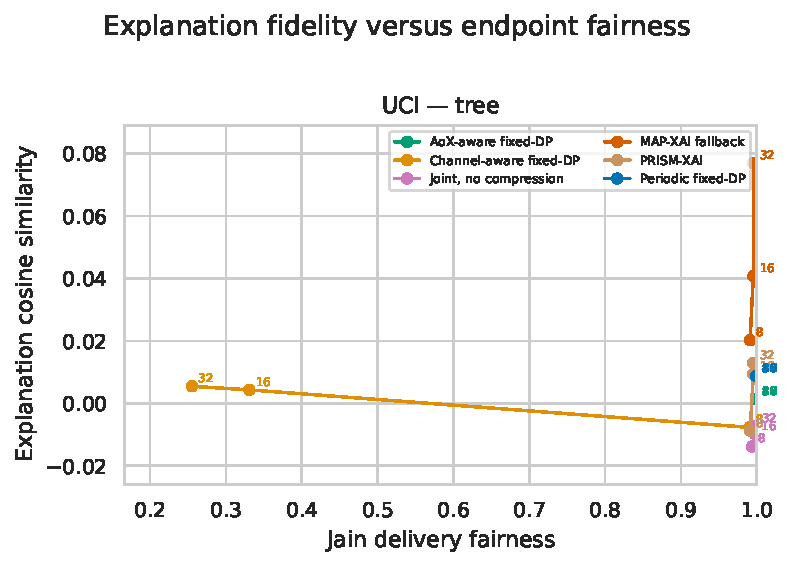
\includegraphics[width=.96\textwidth,height=.82\textheight,keepaspectratio]{../../SERVICE_TRADEOFF_RESULTS/runs/thr_2_cap_16/uci/fairness_reliability.pdf}

\caption{Public-score threshold $\tau=2$, release cap $M=16$, UCI: fairness--reliability plane. This panel should be read with the setting-level quantitative interpretation and the complete tables immediately preceding the figure block.}

\end{figure*}

\clearpage

\begin{figure*}[p]

\centering

\includegraphics[width=.96\textwidth,height=.82\textheight,keepaspectratio]{../../SERVICE_TRADEOFF_RESULTS/runs/thr_2_cap_16/uci/privacy_fidelity.pdf}

\caption{Public-score threshold $\tau=2$, release cap $M=16$, UCI: privacy--fidelity plane. This panel should be read with the setting-level quantitative interpretation and the complete tables immediately preceding the figure block.}

\end{figure*}

\clearpage

\begin{figure*}[p]

\centering

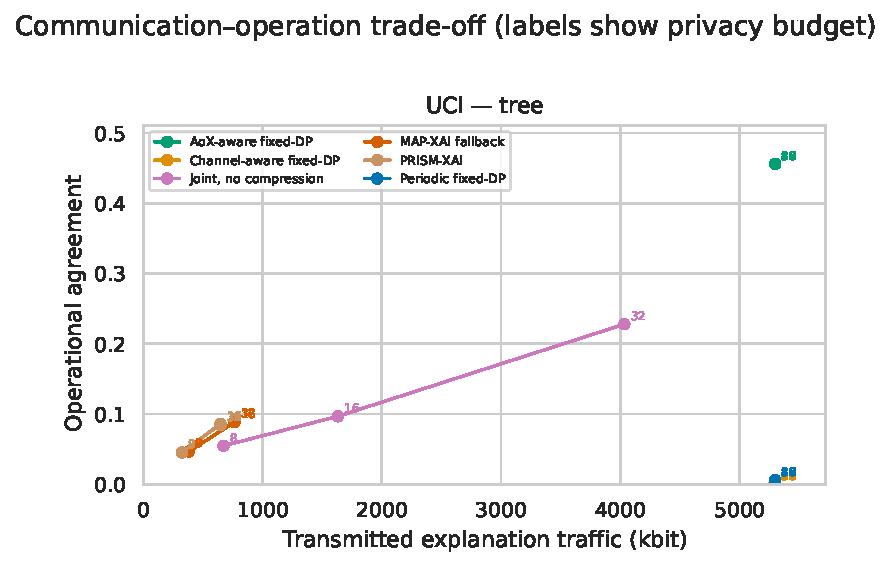
\includegraphics[width=.96\textwidth,height=.82\textheight,keepaspectratio]{../../SERVICE_TRADEOFF_RESULTS/runs/thr_2_cap_16/uci/pareto_bits_fidelity.pdf}

\caption{Public-score threshold $\tau=2$, release cap $M=16$, UCI: traffic--fidelity Pareto plane. This panel should be read with the setting-level quantitative interpretation and the complete tables immediately preceding the figure block.}

\end{figure*}

\clearpage

\begin{figure*}[p]

\centering

\includegraphics[width=.96\textwidth,height=.82\textheight,keepaspectratio]{../../SERVICE_TRADEOFF_RESULTS/runs/thr_2_cap_16/uci/ablation_results.pdf}

\caption{Public-score threshold $\tau=2$, release cap $M=16$, UCI: component ablation. This panel should be read with the setting-level quantitative interpretation and the complete tables immediately preceding the figure block.}

\end{figure*}

\clearpage

\subsubsection{Public-score threshold $\tau=3$, release cap $M=16$}

At this operating point, PRISM-XAI transmits 345.42~kbit versus 407.78~kbit for MAP-XAI-only (aggregate-mean ratio saving 15.29\%). The paired difference is -62.36$\pm$6.82~kbit. PRISM coverage is 0.1312, critical-event recall is 0.0594, and maximum recorded expenditure is 17.777. Relative to MAP-XAI-only, the paired coverage change is -0.00010$\pm$0.00034 and recall change is +0.00244$\pm$0.00227. The descriptive overlap rule holds in 8 of 12 cells. Accordingly, this point is read as a sensitivity point on the service frontier, not a complete matched-service confirmation.

\paragraph{Combined datasets.} The three generated tables below report the full method means, all condition-level values, and paired differences. The five figures that follow provide the corresponding temporal, fairness, privacy, Pareto, and ablation views. Aggregate panels support the setting-level summary above; dataset panels reveal whether that summary is shared by OPSD and UCI rather than being driven by their different endpoint counts.

\begin{table*}[p]\centering\tiny

\caption{Public-score threshold $\tau=3$, release cap $M=16$, Combined datasets: complete generated method table.}

\label{tab:thr_3_cap_16:combined:main}

\resizebox{\linewidth}{!}{% Values are means with 95% Student-t confidence intervals across seeds.
\begin{tabular}{lccccccccccccccc}
\toprule
Dataset & Model & $\epsilon_{\max}$ & Method & Top-$K$ & Cosine & Decision & Recall & Prec. & Abst. & P95 ms & kbit & Spent $\epsilon$ & False int. & bit/correct & Fairness \\
\midrule
OPSD & Tree & 8 & AoX-aware fixed-DP & 0.234 $\pm$ 0.048 & -0.033 $\pm$ 0.028 & 0.119 $\pm$ 0.028 & 0.119 $\pm$ 0.028 & 0.198 $\pm$ 0.054 & 0.721 $\pm$ 0.005 & 6.903 $\pm$ 1.126 & 1560.564 $\pm$ 0.000 & 7.990 $\pm$ 0.000 & 0.183 $\pm$ 0.020 & 35567.482 $\pm$ 10569.818 & 0.999 $\pm$ 0.000 \\
OPSD & Tree & 8 & AoX-aware fixed-DP & 0.238 $\pm$ 0.049 & -0.026 $\pm$ 0.055 & 0.121 $\pm$ 0.026 & 0.121 $\pm$ 0.026 & 0.205 $\pm$ 0.053 & 0.721 $\pm$ 0.005 & 6.903 $\pm$ 1.126 & 1560.564 $\pm$ 0.000 & 7.990 $\pm$ 0.000 & 0.179 $\pm$ 0.023 & 34123.214 $\pm$ 8376.542 & 0.999 $\pm$ 0.000 \\
OPSD & Tree & 8 & Channel-aware fixed-DP & 0.292 $\pm$ 0.037 & -0.041 $\pm$ 0.051 & 0.107 $\pm$ 0.026 & 0.107 $\pm$ 0.026 & 0.217 $\pm$ 0.068 & 0.779 $\pm$ 0.011 & 5.571 $\pm$ 1.784 & 1560.564 $\pm$ 0.000 & 7.990 $\pm$ 0.000 & 0.154 $\pm$ 0.029 & 40860.756 $\pm$ 14126.920 & 0.999 $\pm$ 0.000 \\
OPSD & Tree & 8 & Channel-aware fixed-DP & 0.292 $\pm$ 0.054 & -0.049 $\pm$ 0.064 & 0.111 $\pm$ 0.023 & 0.111 $\pm$ 0.023 & 0.228 $\pm$ 0.066 & 0.779 $\pm$ 0.011 & 5.571 $\pm$ 1.784 & 1560.564 $\pm$ 0.000 & 7.990 $\pm$ 0.000 & 0.149 $\pm$ 0.026 & 37980.855 $\pm$ 12338.094 & 0.999 $\pm$ 0.000 \\
OPSD & Tree & 8 & Joint, no compression & 0.288 $\pm$ 0.064 & -0.030 $\pm$ 0.079 & 0.016 $\pm$ 0.005 & 0.016 $\pm$ 0.005 & 0.193 $\pm$ 0.059 & 0.957 $\pm$ 0.003 & 4.560 $\pm$ 1.811 & 189.900 $\pm$ 0.554 & 7.990 $\pm$ 0.000 & 0.027 $\pm$ 0.005 & 32490.357 $\pm$ 10149.755 & 0.996 $\pm$ 0.002 \\
OPSD & Tree & 8 & Joint, no compression & 0.258 $\pm$ 0.055 & 0.011 $\pm$ 0.094 & 0.019 $\pm$ 0.004 & 0.019 $\pm$ 0.004 & 0.224 $\pm$ 0.044 & 0.957 $\pm$ 0.003 & 4.562 $\pm$ 1.809 & 189.750 $\pm$ 0.566 & 7.990 $\pm$ 0.000 & 0.025 $\pm$ 0.003 & 26079.167 $\pm$ 6335.386 & 0.996 $\pm$ 0.002 \\
OPSD & Tree & 8 & Periodic fixed-DP & 0.241 $\pm$ 0.049 & -0.019 $\pm$ 0.061 & 0.125 $\pm$ 0.020 & 0.125 $\pm$ 0.020 & 0.209 $\pm$ 0.044 & 0.722 $\pm$ 0.006 & 6.303 $\pm$ 1.438 & 1560.564 $\pm$ 0.000 & 7.990 $\pm$ 0.000 & 0.181 $\pm$ 0.021 & 31183.082 $\pm$ 4356.378 & 0.999 $\pm$ 0.000 \\
OPSD & Tree & 8 & Periodic fixed-DP & 0.242 $\pm$ 0.048 & -0.026 $\pm$ 0.082 & 0.135 $\pm$ 0.016 & 0.135 $\pm$ 0.016 & 0.231 $\pm$ 0.037 & 0.722 $\pm$ 0.006 & 6.303 $\pm$ 1.438 & 1560.564 $\pm$ 0.000 & 7.990 $\pm$ 0.000 & 0.169 $\pm$ 0.017 & 28520.235 $\pm$ 3511.595 & 0.999 $\pm$ 0.000 \\
OPSD & Tree & 8 & PRISM-XAI & 0.231 $\pm$ 0.042 & 0.028 $\pm$ 0.075 & 0.025 $\pm$ 0.011 & 0.025 $\pm$ 0.011 & 0.268 $\pm$ 0.127 & 0.929 $\pm$ 0.005 & 4.879 $\pm$ 1.736 & 88.444 $\pm$ 0.568 & 6.067 $\pm$ 0.212 & 0.026 $\pm$ 0.005 & 12196.035 $\pm$ 5705.209 & 0.990 $\pm$ 0.006 \\
OPSD & Tree & 8 & PRISM-XAI & 0.244 $\pm$ 0.039 & 0.030 $\pm$ 0.085 & 0.026 $\pm$ 0.012 & 0.026 $\pm$ 0.012 & 0.274 $\pm$ 0.138 & 0.929 $\pm$ 0.004 & 4.869 $\pm$ 1.744 & 87.922 $\pm$ 0.520 & 5.936 $\pm$ 0.213 & 0.027 $\pm$ 0.007 & 11503.042 $\pm$ 5462.280 & 0.990 $\pm$ 0.006 \\
OPSD & Tree & 8 & MAP-XAI fallback & 0.289 $\pm$ 0.065 & 0.023 $\pm$ 0.079 & 0.028 $\pm$ 0.008 & 0.028 $\pm$ 0.008 & 0.296 $\pm$ 0.082 & 0.929 $\pm$ 0.005 & 4.945 $\pm$ 1.699 & 106.298 $\pm$ 0.291 & 7.786 $\pm$ 0.000 & 0.025 $\pm$ 0.004 & 10222.108 $\pm$ 2661.883 & 0.990 $\pm$ 0.006 \\
OPSD & Tree & 8 & MAP-XAI fallback & 0.267 $\pm$ 0.070 & 0.045 $\pm$ 0.077 & 0.027 $\pm$ 0.007 & 0.027 $\pm$ 0.007 & 0.257 $\pm$ 0.051 & 0.929 $\pm$ 0.005 & 4.948 $\pm$ 1.696 & 106.157 $\pm$ 0.283 & 7.786 $\pm$ 0.000 & 0.028 $\pm$ 0.003 & 10802.437 $\pm$ 2867.714 & 0.990 $\pm$ 0.006 \\
UCI & Tree & 8 & AoX-aware fixed-DP & 0.263 $\pm$ 0.041 & -0.007 $\pm$ 0.009 & 0.457 $\pm$ 0.031 & 0.457 $\pm$ 0.031 & 0.362 $\pm$ 0.024 & 0.003 $\pm$ 0.001 & 7.500 $\pm$ 0.000 & 5300.224 $\pm$ 0.000 & 7.990 $\pm$ 0.000 & 0.557 $\pm$ 0.025 & 14002.896 $\pm$ 1040.243 & 0.999 $\pm$ 0.000 \\
UCI & Tree & 8 & AoX-aware fixed-DP & 0.260 $\pm$ 0.022 & 0.010 $\pm$ 0.055 & 0.455 $\pm$ 0.047 & 0.455 $\pm$ 0.047 & 0.361 $\pm$ 0.038 & 0.003 $\pm$ 0.001 & 7.500 $\pm$ 0.000 & 5300.224 $\pm$ 0.000 & 7.990 $\pm$ 0.000 & 0.557 $\pm$ 0.048 & 14198.303 $\pm$ 1508.274 & 0.999 $\pm$ 0.000 \\
UCI & Tree & 8 & Channel-aware fixed-DP & 0.248 $\pm$ 0.031 & 0.004 $\pm$ 0.012 & 0.001 $\pm$ 0.001 & 0.001 $\pm$ 0.001 & 0.150 $\pm$ 0.151 & 0.999 $\pm$ 0.001 & 4.609 $\pm$ 1.781 & 5295.177 $\pm$ 3.740 & 7.990 $\pm$ 0.000 & 0.001 $\pm$ 0.001 & 4632196.500 $\pm$ 2102650.252 & 0.991 $\pm$ 0.001 \\
UCI & Tree & 8 & Channel-aware fixed-DP & 0.239 $\pm$ 0.030 & -0.020 $\pm$ 0.055 & 0.000 $\pm$ 0.000 & 0.000 $\pm$ 0.000 & 0.117 $\pm$ 0.225 & 0.999 $\pm$ 0.001 & 4.609 $\pm$ 1.781 & 5295.177 $\pm$ 3.740 & 7.990 $\pm$ 0.000 & 0.001 $\pm$ 0.001 & 5296989.000 $\pm$ 41104.572 & 0.991 $\pm$ 0.001 \\
UCI & Tree & 8 & Joint, no compression & 0.286 $\pm$ 0.045 & 0.004 $\pm$ 0.020 & 0.052 $\pm$ 0.005 & 0.052 $\pm$ 0.005 & 0.406 $\pm$ 0.037 & 0.875 $\pm$ 0.003 & 5.123 $\pm$ 1.792 & 672.300 $\pm$ 0.452 & 7.990 $\pm$ 0.000 & 0.053 $\pm$ 0.004 & 15676.175 $\pm$ 1475.621 & 0.994 $\pm$ 0.003 \\
UCI & Tree & 8 & Joint, no compression & 0.229 $\pm$ 0.052 & -0.032 $\pm$ 0.050 & 0.057 $\pm$ 0.007 & 0.057 $\pm$ 0.007 & 0.428 $\pm$ 0.041 & 0.875 $\pm$ 0.003 & 5.131 $\pm$ 1.787 & 672.300 $\pm$ 0.452 & 7.990 $\pm$ 0.000 & 0.052 $\pm$ 0.004 & 14702.786 $\pm$ 2334.488 & 0.994 $\pm$ 0.003 \\
UCI & Tree & 8 & Periodic fixed-DP & 0.259 $\pm$ 0.060 & -0.005 $\pm$ 0.008 & 0.006 $\pm$ 0.001 & 0.006 $\pm$ 0.001 & 0.244 $\pm$ 0.049 & 0.989 $\pm$ 0.001 & 4.596 $\pm$ 1.788 & 5299.318 $\pm$ 1.451 & 7.786 $\pm$ 0.000 & 0.013 $\pm$ 0.002 & 1215103.896 $\pm$ 390671.319 & 0.999 $\pm$ 0.000 \\
UCI & Tree & 8 & Periodic fixed-DP & 0.260 $\pm$ 0.044 & 0.022 $\pm$ 0.070 & 0.005 $\pm$ 0.001 & 0.005 $\pm$ 0.001 & 0.195 $\pm$ 0.050 & 0.989 $\pm$ 0.001 & 4.596 $\pm$ 1.788 & 5299.318 $\pm$ 1.451 & 7.786 $\pm$ 0.000 & 0.015 $\pm$ 0.002 & 1555837.203 $\pm$ 955472.503 & 0.999 $\pm$ 0.000 \\
UCI & Tree & 8 & PRISM-XAI & 0.231 $\pm$ 0.061 & -0.001 $\pm$ 0.013 & 0.043 $\pm$ 0.009 & 0.043 $\pm$ 0.009 & 0.466 $\pm$ 0.081 & 0.909 $\pm$ 0.005 & 5.656 $\pm$ 1.725 & 328.663 $\pm$ 1.360 & 7.081 $\pm$ 0.177 & 0.033 $\pm$ 0.005 & 10019.834 $\pm$ 2488.756 & 0.990 $\pm$ 0.003 \\
UCI & Tree & 8 & PRISM-XAI & 0.245 $\pm$ 0.047 & -0.007 $\pm$ 0.082 & 0.045 $\pm$ 0.007 & 0.045 $\pm$ 0.007 & 0.507 $\pm$ 0.071 & 0.910 $\pm$ 0.005 & 5.163 $\pm$ 1.785 & 325.833 $\pm$ 1.364 & 7.052 $\pm$ 0.147 & 0.030 $\pm$ 0.006 & 9029.695 $\pm$ 1367.291 & 0.991 $\pm$ 0.002 \\
UCI & Tree & 8 & MAP-XAI fallback & 0.202 $\pm$ 0.058 & 0.011 $\pm$ 0.012 & 0.041 $\pm$ 0.005 & 0.041 $\pm$ 0.005 & 0.453 $\pm$ 0.045 & 0.909 $\pm$ 0.005 & 5.677 $\pm$ 1.704 & 381.702 $\pm$ 0.092 & 7.786 $\pm$ 0.000 & 0.034 $\pm$ 0.003 & 11391.295 $\pm$ 1487.072 & 0.990 $\pm$ 0.003 \\
UCI & Tree & 8 & MAP-XAI fallback & 0.206 $\pm$ 0.051 & 0.062 $\pm$ 0.058 & 0.048 $\pm$ 0.010 & 0.048 $\pm$ 0.010 & 0.505 $\pm$ 0.102 & 0.910 $\pm$ 0.005 & 4.861 $\pm$ 1.663 & 381.256 $\pm$ 0.293 & 7.786 $\pm$ 0.000 & 0.033 $\pm$ 0.007 & 10444.880 $\pm$ 2673.464 & 0.991 $\pm$ 0.002 \\
\bottomrule
\end{tabular}
}

\end{table*}\clearpage

\begin{table*}[p]\centering\tiny

\caption{Public-score threshold $\tau=3$, release cap $M=16$, Combined datasets: complete condition-level generated table.}

\label{tab:thr_3_cap_16:combined:conditions}

\resizebox{\textwidth}{!}{\begin{tabular}{llllccccccccccc}
\toprule
Dataset & Model & $\epsilon_{\max}$ & Method & kbit & Top-$K$ & Random Top-$K$ & Cosine & Decision & Recall & Precision & Coverage & Abstain & False int. & Spent $\epsilon$ \\
\midrule
OPSD & Tree & 8 & Joint, no compression & 189.900 $\pm$ 0.554 & 0.288 $\pm$ 0.064 & 0.250 $\pm$ 0.000 & -0.030 $\pm$ 0.079 & 0.016 $\pm$ 0.005 & 0.016 $\pm$ 0.005 & 0.193 $\pm$ 0.059 & 0.043 $\pm$ 0.003 & 0.957 $\pm$ 0.003 & 0.027 $\pm$ 0.005 & 7.990 $\pm$ 0.000 \\
OPSD & Tree & 8 & Joint, no compression & 189.750 $\pm$ 0.566 & 0.258 $\pm$ 0.055 & 0.250 $\pm$ 0.000 & 0.011 $\pm$ 0.094 & 0.019 $\pm$ 0.004 & 0.019 $\pm$ 0.004 & 0.224 $\pm$ 0.044 & 0.043 $\pm$ 0.003 & 0.957 $\pm$ 0.003 & 0.025 $\pm$ 0.003 & 7.990 $\pm$ 0.000 \\
OPSD & Tree & 8 & Periodic fixed-DP & 1560.564 $\pm$ 0.000 & 0.241 $\pm$ 0.049 & 0.250 $\pm$ 0.000 & -0.019 $\pm$ 0.061 & 0.125 $\pm$ 0.020 & 0.125 $\pm$ 0.020 & 0.209 $\pm$ 0.044 & 0.278 $\pm$ 0.006 & 0.722 $\pm$ 0.006 & 0.181 $\pm$ 0.021 & 7.990 $\pm$ 0.000 \\
OPSD & Tree & 8 & Periodic fixed-DP & 1560.564 $\pm$ 0.000 & 0.242 $\pm$ 0.048 & 0.250 $\pm$ 0.000 & -0.026 $\pm$ 0.082 & 0.135 $\pm$ 0.016 & 0.135 $\pm$ 0.016 & 0.231 $\pm$ 0.037 & 0.278 $\pm$ 0.006 & 0.722 $\pm$ 0.006 & 0.169 $\pm$ 0.017 & 7.990 $\pm$ 0.000 \\
OPSD & Tree & 8 & PRISM-XAI & 88.444 $\pm$ 0.568 & 0.231 $\pm$ 0.042 & 0.250 $\pm$ 0.000 & 0.028 $\pm$ 0.075 & 0.025 $\pm$ 0.011 & 0.025 $\pm$ 0.011 & 0.268 $\pm$ 0.127 & 0.071 $\pm$ 0.005 & 0.929 $\pm$ 0.005 & 0.026 $\pm$ 0.005 & 6.067 $\pm$ 0.212 \\
OPSD & Tree & 8 & PRISM-XAI & 87.922 $\pm$ 0.520 & 0.244 $\pm$ 0.039 & 0.250 $\pm$ 0.000 & 0.030 $\pm$ 0.085 & 0.026 $\pm$ 0.012 & 0.026 $\pm$ 0.012 & 0.274 $\pm$ 0.138 & 0.071 $\pm$ 0.004 & 0.929 $\pm$ 0.004 & 0.027 $\pm$ 0.007 & 5.936 $\pm$ 0.213 \\
OPSD & Tree & 16 & Joint, no compression & 459.900 $\pm$ 0.750 & 0.232 $\pm$ 0.065 & 0.250 $\pm$ 0.000 & 0.059 $\pm$ 0.048 & 0.038 $\pm$ 0.009 & 0.038 $\pm$ 0.009 & 0.222 $\pm$ 0.049 & 0.088 $\pm$ 0.004 & 0.912 $\pm$ 0.004 & 0.049 $\pm$ 0.005 & 15.997 $\pm$ 0.000 \\
OPSD & Tree & 16 & Joint, no compression & 460.050 $\pm$ 0.724 & 0.241 $\pm$ 0.055 & 0.250 $\pm$ 0.000 & 0.061 $\pm$ 0.052 & 0.039 $\pm$ 0.008 & 0.039 $\pm$ 0.008 & 0.241 $\pm$ 0.042 & 0.088 $\pm$ 0.004 & 0.912 $\pm$ 0.004 & 0.045 $\pm$ 0.004 & 15.997 $\pm$ 0.000 \\
OPSD & Tree & 16 & Periodic fixed-DP & 5112.594 $\pm$ 0.000 & 0.249 $\pm$ 0.022 & 0.250 $\pm$ 0.000 & -0.009 $\pm$ 0.045 & 0.450 $\pm$ 0.062 & 0.450 $\pm$ 0.062 & 0.237 $\pm$ 0.042 & 0.985 $\pm$ 0.002 & 0.015 $\pm$ 0.002 & 0.551 $\pm$ 0.057 & 15.997 $\pm$ 0.000 \\
OPSD & Tree & 16 & Periodic fixed-DP & 5112.594 $\pm$ 0.000 & 0.243 $\pm$ 0.019 & 0.250 $\pm$ 0.000 & -0.012 $\pm$ 0.050 & 0.463 $\pm$ 0.047 & 0.463 $\pm$ 0.047 & 0.240 $\pm$ 0.028 & 0.985 $\pm$ 0.002 & 0.015 $\pm$ 0.002 & 0.547 $\pm$ 0.036 & 15.997 $\pm$ 0.000 \\
OPSD & Tree & 16 & PRISM-XAI & 177.011 $\pm$ 0.621 & 0.255 $\pm$ 0.065 & 0.250 $\pm$ 0.000 & 0.062 $\pm$ 0.075 & 0.049 $\pm$ 0.016 & 0.049 $\pm$ 0.016 & 0.290 $\pm$ 0.110 & 0.133 $\pm$ 0.003 & 0.867 $\pm$ 0.003 & 0.047 $\pm$ 0.010 & 15.620 $\pm$ 0.000 \\
OPSD & Tree & 16 & PRISM-XAI & 176.182 $\pm$ 0.595 & 0.244 $\pm$ 0.039 & 0.250 $\pm$ 0.000 & 0.080 $\pm$ 0.081 & 0.049 $\pm$ 0.013 & 0.049 $\pm$ 0.013 & 0.287 $\pm$ 0.097 & 0.132 $\pm$ 0.004 & 0.868 $\pm$ 0.004 & 0.048 $\pm$ 0.009 & 15.620 $\pm$ 0.000 \\
OPSD & Tree & 32 & Joint, no compression & 1140.900 $\pm$ 7.953 & 0.235 $\pm$ 0.064 & 0.250 $\pm$ 0.000 & -0.031 $\pm$ 0.089 & 0.074 $\pm$ 0.015 & 0.074 $\pm$ 0.015 & 0.205 $\pm$ 0.039 & 0.157 $\pm$ 0.006 & 0.843 $\pm$ 0.006 & 0.107 $\pm$ 0.009 & 31.999 $\pm$ 0.000 \\
OPSD & Tree & 32 & Joint, no compression & 1140.900 $\pm$ 7.953 & 0.282 $\pm$ 0.054 & 0.250 $\pm$ 0.000 & -0.044 $\pm$ 0.076 & 0.080 $\pm$ 0.011 & 0.080 $\pm$ 0.011 & 0.227 $\pm$ 0.052 & 0.158 $\pm$ 0.006 & 0.842 $\pm$ 0.006 & 0.105 $\pm$ 0.015 & 31.999 $\pm$ 0.000 \\
OPSD & Tree & 32 & Periodic fixed-DP & 5299.836 $\pm$ 0.625 & 0.249 $\pm$ 0.022 & 0.250 $\pm$ 0.000 & -0.009 $\pm$ 0.044 & 0.458 $\pm$ 0.066 & 0.458 $\pm$ 0.066 & 0.237 $\pm$ 0.045 & 1.000 $\pm$ 0.000 & 0.000 $\pm$ 0.000 & 0.562 $\pm$ 0.062 & 16.371 $\pm$ 0.000 \\
OPSD & Tree & 32 & Periodic fixed-DP & 5299.836 $\pm$ 0.625 & 0.244 $\pm$ 0.019 & 0.250 $\pm$ 0.000 & -0.012 $\pm$ 0.050 & 0.471 $\pm$ 0.049 & 0.471 $\pm$ 0.049 & 0.240 $\pm$ 0.029 & 1.000 $\pm$ 0.000 & 0.000 $\pm$ 0.000 & 0.559 $\pm$ 0.039 & 16.371 $\pm$ 0.000 \\
OPSD & Tree & 32 & PRISM-XAI & 176.950 $\pm$ 0.602 & 0.317 $\pm$ 0.078 & 0.250 $\pm$ 0.000 & 0.217 $\pm$ 0.056 & 0.065 $\pm$ 0.016 & 0.065 $\pm$ 0.016 & 0.389 $\pm$ 0.094 & 0.133 $\pm$ 0.003 & 0.867 $\pm$ 0.003 & 0.038 $\pm$ 0.005 & 31.175 $\pm$ 0.000 \\
OPSD & Tree & 32 & PRISM-XAI & 175.967 $\pm$ 0.530 & 0.283 $\pm$ 0.060 & 0.250 $\pm$ 0.000 & 0.255 $\pm$ 0.060 & 0.069 $\pm$ 0.013 & 0.069 $\pm$ 0.013 & 0.404 $\pm$ 0.078 & 0.132 $\pm$ 0.004 & 0.868 $\pm$ 0.004 & 0.038 $\pm$ 0.006 & 31.175 $\pm$ 0.000 \\
UCI & Tree & 8 & Joint, no compression & 672.300 $\pm$ 0.452 & 0.286 $\pm$ 0.045 & 0.250 $\pm$ 0.000 & 0.004 $\pm$ 0.020 & 0.052 $\pm$ 0.005 & 0.052 $\pm$ 0.005 & 0.406 $\pm$ 0.037 & 0.125 $\pm$ 0.003 & 0.875 $\pm$ 0.003 & 0.053 $\pm$ 0.004 & 7.990 $\pm$ 0.000 \\
UCI & Tree & 8 & Joint, no compression & 672.300 $\pm$ 0.452 & 0.229 $\pm$ 0.052 & 0.250 $\pm$ 0.000 & -0.032 $\pm$ 0.050 & 0.057 $\pm$ 0.007 & 0.057 $\pm$ 0.007 & 0.428 $\pm$ 0.041 & 0.125 $\pm$ 0.003 & 0.875 $\pm$ 0.003 & 0.052 $\pm$ 0.004 & 7.990 $\pm$ 0.000 \\
UCI & Tree & 8 & Periodic fixed-DP & 5299.318 $\pm$ 1.451 & 0.259 $\pm$ 0.060 & 0.250 $\pm$ 0.000 & -0.005 $\pm$ 0.008 & 0.006 $\pm$ 0.001 & 0.006 $\pm$ 0.001 & 0.244 $\pm$ 0.049 & 0.011 $\pm$ 0.001 & 0.989 $\pm$ 0.001 & 0.013 $\pm$ 0.002 & 7.786 $\pm$ 0.000 \\
UCI & Tree & 8 & Periodic fixed-DP & 5299.318 $\pm$ 1.451 & 0.260 $\pm$ 0.044 & 0.250 $\pm$ 0.000 & 0.022 $\pm$ 0.070 & 0.005 $\pm$ 0.001 & 0.005 $\pm$ 0.001 & 0.195 $\pm$ 0.050 & 0.011 $\pm$ 0.001 & 0.989 $\pm$ 0.001 & 0.015 $\pm$ 0.002 & 7.786 $\pm$ 0.000 \\
UCI & Tree & 8 & PRISM-XAI & 328.663 $\pm$ 1.360 & 0.231 $\pm$ 0.061 & 0.250 $\pm$ 0.000 & -0.001 $\pm$ 0.013 & 0.043 $\pm$ 0.009 & 0.043 $\pm$ 0.009 & 0.466 $\pm$ 0.081 & 0.091 $\pm$ 0.005 & 0.909 $\pm$ 0.005 & 0.033 $\pm$ 0.005 & 7.081 $\pm$ 0.177 \\
UCI & Tree & 8 & PRISM-XAI & 325.833 $\pm$ 1.364 & 0.245 $\pm$ 0.047 & 0.250 $\pm$ 0.000 & -0.007 $\pm$ 0.082 & 0.045 $\pm$ 0.007 & 0.045 $\pm$ 0.007 & 0.507 $\pm$ 0.071 & 0.090 $\pm$ 0.005 & 0.910 $\pm$ 0.005 & 0.030 $\pm$ 0.006 & 7.052 $\pm$ 0.147 \\
UCI & Tree & 16 & Joint, no compression & 1632.150 $\pm$ 0.339 & 0.216 $\pm$ 0.041 & 0.250 $\pm$ 0.000 & 0.001 $\pm$ 0.012 & 0.094 $\pm$ 0.005 & 0.094 $\pm$ 0.005 & 0.330 $\pm$ 0.024 & 0.228 $\pm$ 0.005 & 0.772 $\pm$ 0.005 & 0.133 $\pm$ 0.010 & 15.997 $\pm$ 0.000 \\
UCI & Tree & 16 & Joint, no compression & 1632.600 $\pm$ 0.554 & 0.204 $\pm$ 0.011 & 0.250 $\pm$ 0.000 & -0.021 $\pm$ 0.033 & 0.099 $\pm$ 0.016 & 0.099 $\pm$ 0.016 & 0.347 $\pm$ 0.054 & 0.228 $\pm$ 0.005 & 0.772 $\pm$ 0.005 & 0.128 $\pm$ 0.011 & 15.997 $\pm$ 0.000 \\
UCI & Tree & 16 & Periodic fixed-DP & 5299.318 $\pm$ 1.451 & 0.259 $\pm$ 0.060 & 0.250 $\pm$ 0.000 & -0.005 $\pm$ 0.008 & 0.006 $\pm$ 0.001 & 0.006 $\pm$ 0.001 & 0.244 $\pm$ 0.049 & 0.011 $\pm$ 0.001 & 0.989 $\pm$ 0.001 & 0.013 $\pm$ 0.002 & 7.786 $\pm$ 0.000 \\
UCI & Tree & 16 & Periodic fixed-DP & 5299.318 $\pm$ 1.451 & 0.260 $\pm$ 0.044 & 0.250 $\pm$ 0.000 & 0.022 $\pm$ 0.070 & 0.005 $\pm$ 0.001 & 0.005 $\pm$ 0.001 & 0.195 $\pm$ 0.050 & 0.011 $\pm$ 0.001 & 0.989 $\pm$ 0.001 & 0.015 $\pm$ 0.002 & 7.786 $\pm$ 0.000 \\
UCI & Tree & 16 & PRISM-XAI & 656.329 $\pm$ 1.493 & 0.313 $\pm$ 0.040 & 0.250 $\pm$ 0.000 & 0.015 $\pm$ 0.023 & 0.081 $\pm$ 0.007 & 0.081 $\pm$ 0.007 & 0.445 $\pm$ 0.042 & 0.183 $\pm$ 0.005 & 0.817 $\pm$ 0.005 & 0.070 $\pm$ 0.007 & 15.620 $\pm$ 0.000 \\
UCI & Tree & 16 & PRISM-XAI & 648.965 $\pm$ 1.563 & 0.238 $\pm$ 0.050 & 0.250 $\pm$ 0.000 & -0.027 $\pm$ 0.047 & 0.082 $\pm$ 0.013 & 0.082 $\pm$ 0.013 & 0.471 $\pm$ 0.071 & 0.182 $\pm$ 0.004 & 0.818 $\pm$ 0.004 & 0.064 $\pm$ 0.010 & 15.620 $\pm$ 0.000 \\
UCI & Tree & 32 & Joint, no compression & 4034.550 $\pm$ 5.034 & 0.246 $\pm$ 0.031 & 0.250 $\pm$ 0.000 & -0.002 $\pm$ 0.015 & 0.228 $\pm$ 0.013 & 0.228 $\pm$ 0.013 & 0.361 $\pm$ 0.028 & 0.537 $\pm$ 0.009 & 0.463 $\pm$ 0.009 & 0.279 $\pm$ 0.017 & 31.999 $\pm$ 0.000 \\
UCI & Tree & 32 & Joint, no compression & 4034.550 $\pm$ 5.034 & 0.241 $\pm$ 0.033 & 0.250 $\pm$ 0.000 & -0.012 $\pm$ 0.030 & 0.228 $\pm$ 0.028 & 0.228 $\pm$ 0.028 & 0.360 $\pm$ 0.047 & 0.530 $\pm$ 0.010 & 0.470 $\pm$ 0.010 & 0.280 $\pm$ 0.026 & 31.999 $\pm$ 0.000 \\
UCI & Tree & 32 & Periodic fixed-DP & 5299.318 $\pm$ 1.451 & 0.259 $\pm$ 0.060 & 0.250 $\pm$ 0.000 & -0.005 $\pm$ 0.008 & 0.006 $\pm$ 0.001 & 0.006 $\pm$ 0.001 & 0.244 $\pm$ 0.049 & 0.011 $\pm$ 0.001 & 0.989 $\pm$ 0.001 & 0.013 $\pm$ 0.002 & 7.786 $\pm$ 0.000 \\
UCI & Tree & 32 & Periodic fixed-DP & 5299.318 $\pm$ 1.451 & 0.260 $\pm$ 0.044 & 0.250 $\pm$ 0.000 & 0.022 $\pm$ 0.070 & 0.005 $\pm$ 0.001 & 0.005 $\pm$ 0.001 & 0.195 $\pm$ 0.050 & 0.011 $\pm$ 0.001 & 0.989 $\pm$ 0.001 & 0.015 $\pm$ 0.002 & 7.786 $\pm$ 0.000 \\
UCI & Tree & 32 & PRISM-XAI & 654.773 $\pm$ 1.193 & 0.343 $\pm$ 0.070 & 0.250 $\pm$ 0.000 & 0.019 $\pm$ 0.021 & 0.085 $\pm$ 0.008 & 0.085 $\pm$ 0.008 & 0.556 $\pm$ 0.045 & 0.181 $\pm$ 0.003 & 0.819 $\pm$ 0.003 & 0.048 $\pm$ 0.007 & 31.175 $\pm$ 0.000 \\
UCI & Tree & 32 & PRISM-XAI & 648.024 $\pm$ 1.912 & 0.281 $\pm$ 0.061 & 0.250 $\pm$ 0.000 & -0.049 $\pm$ 0.057 & 0.092 $\pm$ 0.010 & 0.092 $\pm$ 0.010 & 0.595 $\pm$ 0.069 & 0.176 $\pm$ 0.005 & 0.824 $\pm$ 0.005 & 0.044 $\pm$ 0.009 & 31.175 $\pm$ 0.000 \\
\bottomrule
\end{tabular}
}

\end{table*}\clearpage

\begin{table*}[p]\centering\tiny

\caption{Public-score threshold $\tau=3$, release cap $M=16$, Combined datasets: complete generated paired comparisons.}

\label{tab:thr_3_cap_16:combined:paired}

\resizebox{\textwidth}{!}{\begin{tabular}{llcccc}
\toprule
Dataset & Baseline & Delta kbit & Delta Top-$K$ & Delta recall & Delta fairness \\
\midrule
OPSD & AoX-aware fixed-DP & -1472.120 $\pm$ 0.568 & -0.002 $\pm$ 0.037 & -0.094 $\pm$ 0.036 & -0.009 $\pm$ 0.005 \\
OPSD & AoX-aware fixed-DP & -4922.902 $\pm$ 5.453 & 0.002 $\pm$ 0.065 & -0.353 $\pm$ 0.085 & -0.004 $\pm$ 0.002 \\
OPSD & AoX-aware fixed-DP & -5123.274 $\pm$ 0.602 & 0.064 $\pm$ 0.095 & -0.348 $\pm$ 0.082 & -0.004 $\pm$ 0.002 \\
OPSD & AoX-aware fixed-DP & -1472.642 $\pm$ 0.520 & 0.006 $\pm$ 0.074 & -0.094 $\pm$ 0.032 & -0.009 $\pm$ 0.005 \\
OPSD & AoX-aware fixed-DP & -4923.731 $\pm$ 5.465 & -0.009 $\pm$ 0.028 & -0.365 $\pm$ 0.064 & -0.004 $\pm$ 0.002 \\
OPSD & AoX-aware fixed-DP & -5124.257 $\pm$ 0.530 & 0.031 $\pm$ 0.068 & -0.356 $\pm$ 0.063 & -0.004 $\pm$ 0.002 \\
OPSD & Channel-aware fixed-DP & -1472.120 $\pm$ 0.568 & -0.061 $\pm$ 0.040 & -0.082 $\pm$ 0.032 & -0.009 $\pm$ 0.006 \\
OPSD & Channel-aware fixed-DP & -4509.598 $\pm$ 13.076 & -0.006 $\pm$ 0.066 & -0.353 $\pm$ 0.099 & 0.058 $\pm$ 0.005 \\
OPSD & Channel-aware fixed-DP & -5123.274 $\pm$ 0.602 & 0.059 $\pm$ 0.086 & -0.370 $\pm$ 0.105 & 0.089 $\pm$ 0.006 \\
OPSD & Channel-aware fixed-DP & -1472.642 $\pm$ 0.520 & -0.048 $\pm$ 0.081 & -0.085 $\pm$ 0.029 & -0.009 $\pm$ 0.006 \\
OPSD & Channel-aware fixed-DP & -4510.427 $\pm$ 13.230 & -0.014 $\pm$ 0.034 & -0.370 $\pm$ 0.095 & 0.058 $\pm$ 0.005 \\
OPSD & Channel-aware fixed-DP & -5124.257 $\pm$ 0.530 & 0.026 $\pm$ 0.060 & -0.387 $\pm$ 0.094 & 0.089 $\pm$ 0.006 \\
OPSD & Joint, no compression & -101.456 $\pm$ 0.717 & -0.057 $\pm$ 0.086 & 0.009 $\pm$ 0.011 & -0.005 $\pm$ 0.005 \\
OPSD & Joint, no compression & -282.889 $\pm$ 1.277 & 0.024 $\pm$ 0.088 & 0.011 $\pm$ 0.020 & -0.002 $\pm$ 0.002 \\
OPSD & Joint, no compression & -963.950 $\pm$ 8.300 & 0.081 $\pm$ 0.110 & -0.009 $\pm$ 0.026 & -0.003 $\pm$ 0.002 \\
OPSD & Joint, no compression & -101.828 $\pm$ 0.658 & -0.014 $\pm$ 0.072 & 0.007 $\pm$ 0.012 & -0.006 $\pm$ 0.005 \\
OPSD & Joint, no compression & -283.868 $\pm$ 1.164 & 0.003 $\pm$ 0.051 & 0.011 $\pm$ 0.015 & -0.002 $\pm$ 0.002 \\
OPSD & Joint, no compression & -964.933 $\pm$ 8.317 & 0.001 $\pm$ 0.091 & -0.011 $\pm$ 0.019 & -0.003 $\pm$ 0.002 \\
OPSD & Periodic fixed-DP & -1472.120 $\pm$ 0.568 & -0.009 $\pm$ 0.039 & -0.100 $\pm$ 0.027 & -0.009 $\pm$ 0.006 \\
OPSD & Periodic fixed-DP & -4935.583 $\pm$ 0.621 & 0.006 $\pm$ 0.073 & -0.402 $\pm$ 0.071 & -0.004 $\pm$ 0.002 \\
OPSD & Periodic fixed-DP & -5122.886 $\pm$ 0.681 & 0.068 $\pm$ 0.082 & -0.393 $\pm$ 0.071 & -0.004 $\pm$ 0.002 \\
OPSD & Periodic fixed-DP & -1472.642 $\pm$ 0.520 & 0.002 $\pm$ 0.063 & -0.108 $\pm$ 0.022 & -0.009 $\pm$ 0.006 \\
OPSD & Periodic fixed-DP & -4936.412 $\pm$ 0.595 & 0.001 $\pm$ 0.039 & -0.413 $\pm$ 0.054 & -0.004 $\pm$ 0.002 \\
OPSD & Periodic fixed-DP & -5123.869 $\pm$ 0.738 & 0.039 $\pm$ 0.068 & -0.402 $\pm$ 0.053 & -0.004 $\pm$ 0.002 \\
OPSD & MAP-XAI fallback & -17.854 $\pm$ 0.558 & -0.058 $\pm$ 0.062 & -0.003 $\pm$ 0.007 & 0.000 $\pm$ 0.000 \\
OPSD & MAP-XAI fallback & -37.287 $\pm$ 0.637 & 0.025 $\pm$ 0.049 & 0.001 $\pm$ 0.008 & 0.000 $\pm$ 0.000 \\
OPSD & MAP-XAI fallback & -37.328 $\pm$ 0.611 & 0.037 $\pm$ 0.050 & 0.007 $\pm$ 0.010 & 0.000 $\pm$ 0.000 \\
OPSD & MAP-XAI fallback & -18.235 $\pm$ 0.524 & -0.023 $\pm$ 0.076 & -0.000 $\pm$ 0.008 & 0.000 $\pm$ 0.000 \\
OPSD & MAP-XAI fallback & -37.954 $\pm$ 0.593 & 0.018 $\pm$ 0.059 & 0.003 $\pm$ 0.008 & 0.000 $\pm$ 0.000 \\
OPSD & MAP-XAI fallback & -38.087 $\pm$ 0.533 & 0.046 $\pm$ 0.041 & 0.011 $\pm$ 0.010 & 0.000 $\pm$ 0.000 \\
UCI & AoX-aware fixed-DP & -4971.561 $\pm$ 1.360 & -0.033 $\pm$ 0.085 & -0.414 $\pm$ 0.028 & -0.009 $\pm$ 0.003 \\
UCI & AoX-aware fixed-DP & -4643.895 $\pm$ 1.493 & 0.049 $\pm$ 0.050 & -0.376 $\pm$ 0.029 & -0.003 $\pm$ 0.001 \\
UCI & AoX-aware fixed-DP & -4645.451 $\pm$ 1.193 & 0.079 $\pm$ 0.059 & -0.372 $\pm$ 0.030 & -0.003 $\pm$ 0.001 \\
UCI & AoX-aware fixed-DP & -4974.391 $\pm$ 1.364 & -0.016 $\pm$ 0.045 & -0.410 $\pm$ 0.049 & -0.008 $\pm$ 0.002 \\
UCI & AoX-aware fixed-DP & -4651.259 $\pm$ 1.563 & -0.023 $\pm$ 0.046 & -0.372 $\pm$ 0.044 & -0.003 $\pm$ 0.001 \\
UCI & AoX-aware fixed-DP & -4652.200 $\pm$ 1.912 & 0.020 $\pm$ 0.052 & -0.362 $\pm$ 0.051 & -0.003 $\pm$ 0.001 \\
UCI & Channel-aware fixed-DP & -4966.514 $\pm$ 3.919 & -0.018 $\pm$ 0.079 & 0.042 $\pm$ 0.009 & -0.000 $\pm$ 0.002 \\
UCI & Channel-aware fixed-DP & -4643.895 $\pm$ 1.493 & 0.045 $\pm$ 0.059 & 0.080 $\pm$ 0.007 & 0.665 $\pm$ 0.001 \\
UCI & Channel-aware fixed-DP & -4645.451 $\pm$ 1.193 & 0.074 $\pm$ 0.071 & 0.085 $\pm$ 0.009 & 0.741 $\pm$ 0.001 \\
UCI & Channel-aware fixed-DP & -4969.344 $\pm$ 4.185 & 0.006 $\pm$ 0.055 & 0.045 $\pm$ 0.007 & 0.000 $\pm$ 0.002 \\
UCI & Channel-aware fixed-DP & -4651.259 $\pm$ 1.563 & -0.022 $\pm$ 0.058 & 0.082 $\pm$ 0.013 & 0.666 $\pm$ 0.001 \\
UCI & Channel-aware fixed-DP & -4652.200 $\pm$ 1.912 & 0.021 $\pm$ 0.068 & 0.092 $\pm$ 0.011 & 0.741 $\pm$ 0.001 \\
UCI & Joint, no compression & -343.637 $\pm$ 1.641 & -0.055 $\pm$ 0.093 & -0.009 $\pm$ 0.010 & -0.003 $\pm$ 0.003 \\
UCI & Joint, no compression & -975.821 $\pm$ 1.564 & 0.096 $\pm$ 0.035 & -0.013 $\pm$ 0.007 & -0.002 $\pm$ 0.001 \\
UCI & Joint, no compression & -3379.777 $\pm$ 5.671 & 0.097 $\pm$ 0.081 & -0.142 $\pm$ 0.012 & -0.003 $\pm$ 0.001 \\
UCI & Joint, no compression & -346.467 $\pm$ 1.610 & 0.015 $\pm$ 0.070 & -0.012 $\pm$ 0.010 & -0.003 $\pm$ 0.003 \\
UCI & Joint, no compression & -983.635 $\pm$ 1.427 & 0.034 $\pm$ 0.053 & -0.017 $\pm$ 0.024 & -0.002 $\pm$ 0.001 \\
UCI & Joint, no compression & -3386.526 $\pm$ 6.147 & 0.040 $\pm$ 0.071 & -0.135 $\pm$ 0.029 & -0.003 $\pm$ 0.001 \\
UCI & Periodic fixed-DP & -4970.655 $\pm$ 1.984 & -0.029 $\pm$ 0.088 & 0.037 $\pm$ 0.010 & -0.009 $\pm$ 0.003 \\
UCI & Periodic fixed-DP & -4642.989 $\pm$ 2.460 & 0.053 $\pm$ 0.059 & 0.075 $\pm$ 0.007 & -0.003 $\pm$ 0.001 \\
UCI & Periodic fixed-DP & -4644.545 $\pm$ 2.331 & 0.083 $\pm$ 0.082 & 0.080 $\pm$ 0.008 & -0.003 $\pm$ 0.001 \\
UCI & Periodic fixed-DP & -4973.485 $\pm$ 1.727 & -0.016 $\pm$ 0.075 & 0.040 $\pm$ 0.006 & -0.008 $\pm$ 0.002 \\
UCI & Periodic fixed-DP & -4650.353 $\pm$ 1.894 & -0.022 $\pm$ 0.038 & 0.077 $\pm$ 0.012 & -0.003 $\pm$ 0.001 \\
UCI & Periodic fixed-DP & -4651.295 $\pm$ 2.358 & 0.020 $\pm$ 0.078 & 0.087 $\pm$ 0.009 & -0.003 $\pm$ 0.001 \\
UCI & MAP-XAI fallback & -53.039 $\pm$ 1.350 & 0.029 $\pm$ 0.074 & 0.002 $\pm$ 0.006 & 0.000 $\pm$ 0.000 \\
UCI & MAP-XAI fallback & -109.291 $\pm$ 1.508 & 0.053 $\pm$ 0.050 & -0.000 $\pm$ 0.005 & 0.000 $\pm$ 0.000 \\
UCI & MAP-XAI fallback & -110.785 $\pm$ 1.251 & 0.052 $\pm$ 0.090 & 0.001 $\pm$ 0.009 & 0.000 $\pm$ 0.000 \\
UCI & MAP-XAI fallback & -55.422 $\pm$ 1.449 & 0.039 $\pm$ 0.039 & -0.003 $\pm$ 0.007 & 0.000 $\pm$ 0.000 \\
UCI & MAP-XAI fallback & -116.127 $\pm$ 1.715 & 0.008 $\pm$ 0.046 & -0.002 $\pm$ 0.009 & 0.000 $\pm$ 0.000 \\
UCI & MAP-XAI fallback & -116.946 $\pm$ 2.015 & 0.012 $\pm$ 0.040 & 0.014 $\pm$ 0.012 & -0.000 $\pm$ 0.001 \\
\bottomrule
\end{tabular}
}

\end{table*}\clearpage

\begin{figure*}[p]

\centering

\includegraphics[width=.96\textwidth,height=.82\textheight,keepaspectratio]{../../SERVICE_TRADEOFF_RESULTS/runs/thr_3_cap_16/regime_trace.pdf}

\caption{Public-score threshold $\tau=3$, release cap $M=16$, Combined datasets: representative regime trace. This panel should be read with the setting-level quantitative interpretation and the complete tables immediately preceding the figure block.}

\end{figure*}

\clearpage

\begin{figure*}[p]

\centering

\includegraphics[width=.96\textwidth,height=.82\textheight,keepaspectratio]{../../SERVICE_TRADEOFF_RESULTS/runs/thr_3_cap_16/fairness_reliability.pdf}

\caption{Public-score threshold $\tau=3$, release cap $M=16$, Combined datasets: fairness--reliability plane. This panel should be read with the setting-level quantitative interpretation and the complete tables immediately preceding the figure block.}

\end{figure*}

\clearpage

\begin{figure*}[p]

\centering

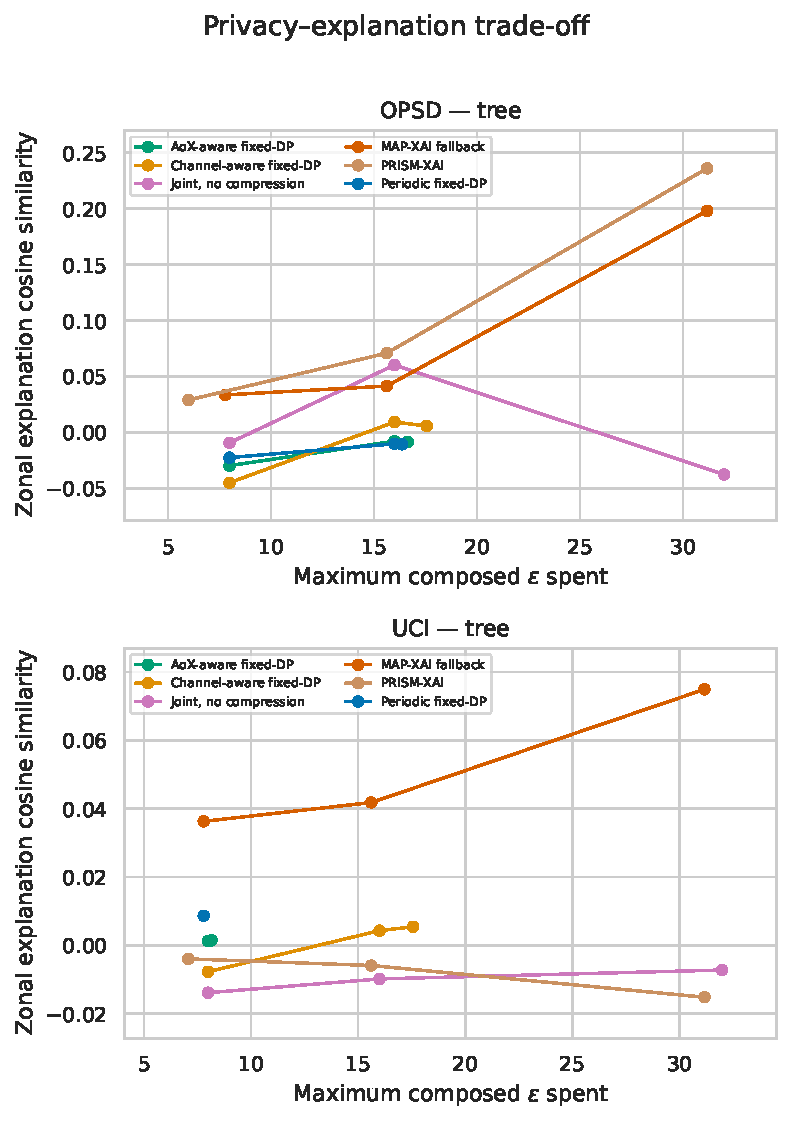
\includegraphics[width=.96\textwidth,height=.82\textheight,keepaspectratio]{../../SERVICE_TRADEOFF_RESULTS/runs/thr_3_cap_16/privacy_fidelity.pdf}

\caption{Public-score threshold $\tau=3$, release cap $M=16$, Combined datasets: privacy--fidelity plane. This panel should be read with the setting-level quantitative interpretation and the complete tables immediately preceding the figure block.}

\end{figure*}

\clearpage

\begin{figure*}[p]

\centering

\includegraphics[width=.96\textwidth,height=.82\textheight,keepaspectratio]{../../SERVICE_TRADEOFF_RESULTS/runs/thr_3_cap_16/pareto_bits_fidelity.pdf}

\caption{Public-score threshold $\tau=3$, release cap $M=16$, Combined datasets: traffic--fidelity Pareto plane. This panel should be read with the setting-level quantitative interpretation and the complete tables immediately preceding the figure block.}

\end{figure*}

\clearpage

\begin{figure*}[p]

\centering

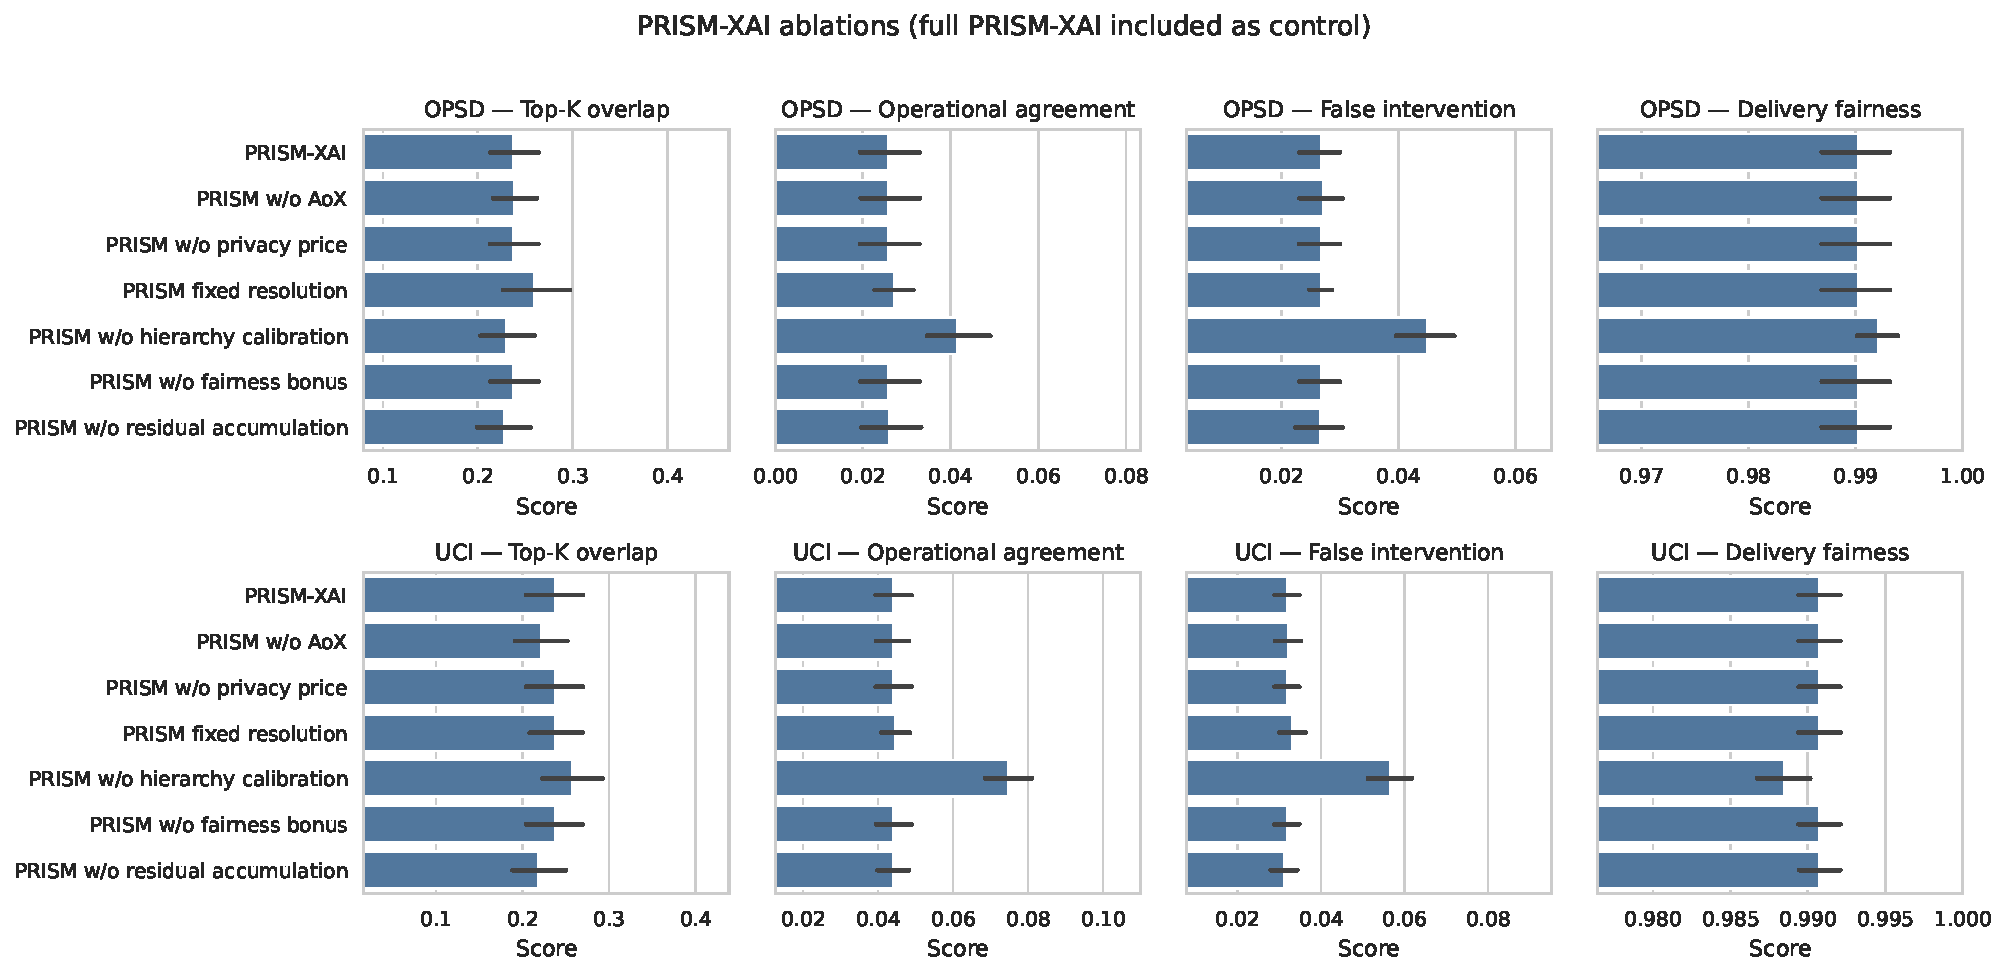
\includegraphics[width=.96\textwidth,height=.82\textheight,keepaspectratio]{../../SERVICE_TRADEOFF_RESULTS/runs/thr_3_cap_16/ablation_results.pdf}

\caption{Public-score threshold $\tau=3$, release cap $M=16$, Combined datasets: component ablation. This panel should be read with the setting-level quantitative interpretation and the complete tables immediately preceding the figure block.}

\end{figure*}

\clearpage

\paragraph{OPSD.} The three generated tables below report the full method means, all condition-level values, and paired differences. The five figures that follow provide the corresponding temporal, fairness, privacy, Pareto, and ablation views. Aggregate panels support the setting-level summary above; dataset panels reveal whether that summary is shared by OPSD and UCI rather than being driven by their different endpoint counts.

\begin{table*}[p]\centering\tiny

\caption{Public-score threshold $\tau=3$, release cap $M=16$, OPSD: complete generated method table.}

\label{tab:thr_3_cap_16:opsd:main}

\resizebox{\linewidth}{!}{% Values are means with 95% Student-t confidence intervals across seeds.
\begin{tabular}{lccccccccccccccc}
\toprule
Dataset & Model & $\epsilon_{\max}$ & Method & Top-$K$ & Cosine & Decision & Recall & Prec. & Abst. & P95 ms & kbit & Spent $\epsilon$ & False int. & bit/correct & Fairness \\
\midrule
OPSD & Tree & 8 & AoX-aware fixed-DP & 0.234 $\pm$ 0.048 & -0.033 $\pm$ 0.028 & 0.119 $\pm$ 0.028 & 0.119 $\pm$ 0.028 & 0.198 $\pm$ 0.054 & 0.721 $\pm$ 0.005 & 6.903 $\pm$ 1.126 & 1560.564 $\pm$ 0.000 & 7.990 $\pm$ 0.000 & 0.183 $\pm$ 0.020 & 35567.482 $\pm$ 10569.818 & 0.999 $\pm$ 0.000 \\
OPSD & Tree & 8 & AoX-aware fixed-DP & 0.238 $\pm$ 0.049 & -0.026 $\pm$ 0.055 & 0.121 $\pm$ 0.026 & 0.121 $\pm$ 0.026 & 0.205 $\pm$ 0.053 & 0.721 $\pm$ 0.005 & 6.903 $\pm$ 1.126 & 1560.564 $\pm$ 0.000 & 7.990 $\pm$ 0.000 & 0.179 $\pm$ 0.023 & 34123.214 $\pm$ 8376.542 & 0.999 $\pm$ 0.000 \\
OPSD & Tree & 8 & Channel-aware fixed-DP & 0.292 $\pm$ 0.037 & -0.041 $\pm$ 0.051 & 0.107 $\pm$ 0.026 & 0.107 $\pm$ 0.026 & 0.217 $\pm$ 0.068 & 0.779 $\pm$ 0.011 & 5.571 $\pm$ 1.784 & 1560.564 $\pm$ 0.000 & 7.990 $\pm$ 0.000 & 0.154 $\pm$ 0.029 & 40860.756 $\pm$ 14126.920 & 0.999 $\pm$ 0.000 \\
OPSD & Tree & 8 & Channel-aware fixed-DP & 0.292 $\pm$ 0.054 & -0.049 $\pm$ 0.064 & 0.111 $\pm$ 0.023 & 0.111 $\pm$ 0.023 & 0.228 $\pm$ 0.066 & 0.779 $\pm$ 0.011 & 5.571 $\pm$ 1.784 & 1560.564 $\pm$ 0.000 & 7.990 $\pm$ 0.000 & 0.149 $\pm$ 0.026 & 37980.855 $\pm$ 12338.094 & 0.999 $\pm$ 0.000 \\
OPSD & Tree & 8 & Joint, no compression & 0.288 $\pm$ 0.064 & -0.030 $\pm$ 0.079 & 0.016 $\pm$ 0.005 & 0.016 $\pm$ 0.005 & 0.193 $\pm$ 0.059 & 0.957 $\pm$ 0.003 & 4.560 $\pm$ 1.811 & 189.900 $\pm$ 0.554 & 7.990 $\pm$ 0.000 & 0.027 $\pm$ 0.005 & 32490.357 $\pm$ 10149.755 & 0.996 $\pm$ 0.002 \\
OPSD & Tree & 8 & Joint, no compression & 0.258 $\pm$ 0.055 & 0.011 $\pm$ 0.094 & 0.019 $\pm$ 0.004 & 0.019 $\pm$ 0.004 & 0.224 $\pm$ 0.044 & 0.957 $\pm$ 0.003 & 4.562 $\pm$ 1.809 & 189.750 $\pm$ 0.566 & 7.990 $\pm$ 0.000 & 0.025 $\pm$ 0.003 & 26079.167 $\pm$ 6335.386 & 0.996 $\pm$ 0.002 \\
OPSD & Tree & 8 & Periodic fixed-DP & 0.241 $\pm$ 0.049 & -0.019 $\pm$ 0.061 & 0.125 $\pm$ 0.020 & 0.125 $\pm$ 0.020 & 0.209 $\pm$ 0.044 & 0.722 $\pm$ 0.006 & 6.303 $\pm$ 1.438 & 1560.564 $\pm$ 0.000 & 7.990 $\pm$ 0.000 & 0.181 $\pm$ 0.021 & 31183.082 $\pm$ 4356.378 & 0.999 $\pm$ 0.000 \\
OPSD & Tree & 8 & Periodic fixed-DP & 0.242 $\pm$ 0.048 & -0.026 $\pm$ 0.082 & 0.135 $\pm$ 0.016 & 0.135 $\pm$ 0.016 & 0.231 $\pm$ 0.037 & 0.722 $\pm$ 0.006 & 6.303 $\pm$ 1.438 & 1560.564 $\pm$ 0.000 & 7.990 $\pm$ 0.000 & 0.169 $\pm$ 0.017 & 28520.235 $\pm$ 3511.595 & 0.999 $\pm$ 0.000 \\
OPSD & Tree & 8 & PRISM-XAI & 0.231 $\pm$ 0.042 & 0.028 $\pm$ 0.075 & 0.025 $\pm$ 0.011 & 0.025 $\pm$ 0.011 & 0.268 $\pm$ 0.127 & 0.929 $\pm$ 0.005 & 4.879 $\pm$ 1.736 & 88.444 $\pm$ 0.568 & 6.067 $\pm$ 0.212 & 0.026 $\pm$ 0.005 & 12196.035 $\pm$ 5705.209 & 0.990 $\pm$ 0.006 \\
OPSD & Tree & 8 & PRISM-XAI & 0.244 $\pm$ 0.039 & 0.030 $\pm$ 0.085 & 0.026 $\pm$ 0.012 & 0.026 $\pm$ 0.012 & 0.274 $\pm$ 0.138 & 0.929 $\pm$ 0.004 & 4.869 $\pm$ 1.744 & 87.922 $\pm$ 0.520 & 5.936 $\pm$ 0.213 & 0.027 $\pm$ 0.007 & 11503.042 $\pm$ 5462.280 & 0.990 $\pm$ 0.006 \\
OPSD & Tree & 8 & MAP-XAI fallback & 0.289 $\pm$ 0.065 & 0.023 $\pm$ 0.079 & 0.028 $\pm$ 0.008 & 0.028 $\pm$ 0.008 & 0.296 $\pm$ 0.082 & 0.929 $\pm$ 0.005 & 4.945 $\pm$ 1.699 & 106.298 $\pm$ 0.291 & 7.786 $\pm$ 0.000 & 0.025 $\pm$ 0.004 & 10222.108 $\pm$ 2661.883 & 0.990 $\pm$ 0.006 \\
OPSD & Tree & 8 & MAP-XAI fallback & 0.267 $\pm$ 0.070 & 0.045 $\pm$ 0.077 & 0.027 $\pm$ 0.007 & 0.027 $\pm$ 0.007 & 0.257 $\pm$ 0.051 & 0.929 $\pm$ 0.005 & 4.948 $\pm$ 1.696 & 106.157 $\pm$ 0.283 & 7.786 $\pm$ 0.000 & 0.028 $\pm$ 0.003 & 10802.437 $\pm$ 2867.714 & 0.990 $\pm$ 0.006 \\
\bottomrule
\end{tabular}
}

\end{table*}\clearpage

\begin{table*}[p]\centering\tiny

\caption{Public-score threshold $\tau=3$, release cap $M=16$, OPSD: complete condition-level generated table.}

\label{tab:thr_3_cap_16:opsd:conditions}

\resizebox{\textwidth}{!}{\begin{tabular}{llllccccccccccc}
\toprule
Dataset & Model & $\epsilon_{\max}$ & Method & kbit & Top-$K$ & Random Top-$K$ & Cosine & Decision & Recall & Precision & Coverage & Abstain & False int. & Spent $\epsilon$ \\
\midrule
OPSD & Tree & 8 & Joint, no compression & 189.900 $\pm$ 0.554 & 0.288 $\pm$ 0.064 & 0.250 $\pm$ 0.000 & -0.030 $\pm$ 0.079 & 0.016 $\pm$ 0.005 & 0.016 $\pm$ 0.005 & 0.193 $\pm$ 0.059 & 0.043 $\pm$ 0.003 & 0.957 $\pm$ 0.003 & 0.027 $\pm$ 0.005 & 7.990 $\pm$ 0.000 \\
OPSD & Tree & 8 & Joint, no compression & 189.750 $\pm$ 0.566 & 0.258 $\pm$ 0.055 & 0.250 $\pm$ 0.000 & 0.011 $\pm$ 0.094 & 0.019 $\pm$ 0.004 & 0.019 $\pm$ 0.004 & 0.224 $\pm$ 0.044 & 0.043 $\pm$ 0.003 & 0.957 $\pm$ 0.003 & 0.025 $\pm$ 0.003 & 7.990 $\pm$ 0.000 \\
OPSD & Tree & 8 & Periodic fixed-DP & 1560.564 $\pm$ 0.000 & 0.241 $\pm$ 0.049 & 0.250 $\pm$ 0.000 & -0.019 $\pm$ 0.061 & 0.125 $\pm$ 0.020 & 0.125 $\pm$ 0.020 & 0.209 $\pm$ 0.044 & 0.278 $\pm$ 0.006 & 0.722 $\pm$ 0.006 & 0.181 $\pm$ 0.021 & 7.990 $\pm$ 0.000 \\
OPSD & Tree & 8 & Periodic fixed-DP & 1560.564 $\pm$ 0.000 & 0.242 $\pm$ 0.048 & 0.250 $\pm$ 0.000 & -0.026 $\pm$ 0.082 & 0.135 $\pm$ 0.016 & 0.135 $\pm$ 0.016 & 0.231 $\pm$ 0.037 & 0.278 $\pm$ 0.006 & 0.722 $\pm$ 0.006 & 0.169 $\pm$ 0.017 & 7.990 $\pm$ 0.000 \\
OPSD & Tree & 8 & PRISM-XAI & 88.444 $\pm$ 0.568 & 0.231 $\pm$ 0.042 & 0.250 $\pm$ 0.000 & 0.028 $\pm$ 0.075 & 0.025 $\pm$ 0.011 & 0.025 $\pm$ 0.011 & 0.268 $\pm$ 0.127 & 0.071 $\pm$ 0.005 & 0.929 $\pm$ 0.005 & 0.026 $\pm$ 0.005 & 6.067 $\pm$ 0.212 \\
OPSD & Tree & 8 & PRISM-XAI & 87.922 $\pm$ 0.520 & 0.244 $\pm$ 0.039 & 0.250 $\pm$ 0.000 & 0.030 $\pm$ 0.085 & 0.026 $\pm$ 0.012 & 0.026 $\pm$ 0.012 & 0.274 $\pm$ 0.138 & 0.071 $\pm$ 0.004 & 0.929 $\pm$ 0.004 & 0.027 $\pm$ 0.007 & 5.936 $\pm$ 0.213 \\
OPSD & Tree & 16 & Joint, no compression & 459.900 $\pm$ 0.750 & 0.232 $\pm$ 0.065 & 0.250 $\pm$ 0.000 & 0.059 $\pm$ 0.048 & 0.038 $\pm$ 0.009 & 0.038 $\pm$ 0.009 & 0.222 $\pm$ 0.049 & 0.088 $\pm$ 0.004 & 0.912 $\pm$ 0.004 & 0.049 $\pm$ 0.005 & 15.997 $\pm$ 0.000 \\
OPSD & Tree & 16 & Joint, no compression & 460.050 $\pm$ 0.724 & 0.241 $\pm$ 0.055 & 0.250 $\pm$ 0.000 & 0.061 $\pm$ 0.052 & 0.039 $\pm$ 0.008 & 0.039 $\pm$ 0.008 & 0.241 $\pm$ 0.042 & 0.088 $\pm$ 0.004 & 0.912 $\pm$ 0.004 & 0.045 $\pm$ 0.004 & 15.997 $\pm$ 0.000 \\
OPSD & Tree & 16 & Periodic fixed-DP & 5112.594 $\pm$ 0.000 & 0.249 $\pm$ 0.022 & 0.250 $\pm$ 0.000 & -0.009 $\pm$ 0.045 & 0.450 $\pm$ 0.062 & 0.450 $\pm$ 0.062 & 0.237 $\pm$ 0.042 & 0.985 $\pm$ 0.002 & 0.015 $\pm$ 0.002 & 0.551 $\pm$ 0.057 & 15.997 $\pm$ 0.000 \\
OPSD & Tree & 16 & Periodic fixed-DP & 5112.594 $\pm$ 0.000 & 0.243 $\pm$ 0.019 & 0.250 $\pm$ 0.000 & -0.012 $\pm$ 0.050 & 0.463 $\pm$ 0.047 & 0.463 $\pm$ 0.047 & 0.240 $\pm$ 0.028 & 0.985 $\pm$ 0.002 & 0.015 $\pm$ 0.002 & 0.547 $\pm$ 0.036 & 15.997 $\pm$ 0.000 \\
OPSD & Tree & 16 & PRISM-XAI & 177.011 $\pm$ 0.621 & 0.255 $\pm$ 0.065 & 0.250 $\pm$ 0.000 & 0.062 $\pm$ 0.075 & 0.049 $\pm$ 0.016 & 0.049 $\pm$ 0.016 & 0.290 $\pm$ 0.110 & 0.133 $\pm$ 0.003 & 0.867 $\pm$ 0.003 & 0.047 $\pm$ 0.010 & 15.620 $\pm$ 0.000 \\
OPSD & Tree & 16 & PRISM-XAI & 176.182 $\pm$ 0.595 & 0.244 $\pm$ 0.039 & 0.250 $\pm$ 0.000 & 0.080 $\pm$ 0.081 & 0.049 $\pm$ 0.013 & 0.049 $\pm$ 0.013 & 0.287 $\pm$ 0.097 & 0.132 $\pm$ 0.004 & 0.868 $\pm$ 0.004 & 0.048 $\pm$ 0.009 & 15.620 $\pm$ 0.000 \\
OPSD & Tree & 32 & Joint, no compression & 1140.900 $\pm$ 7.953 & 0.235 $\pm$ 0.064 & 0.250 $\pm$ 0.000 & -0.031 $\pm$ 0.089 & 0.074 $\pm$ 0.015 & 0.074 $\pm$ 0.015 & 0.205 $\pm$ 0.039 & 0.157 $\pm$ 0.006 & 0.843 $\pm$ 0.006 & 0.107 $\pm$ 0.009 & 31.999 $\pm$ 0.000 \\
OPSD & Tree & 32 & Joint, no compression & 1140.900 $\pm$ 7.953 & 0.282 $\pm$ 0.054 & 0.250 $\pm$ 0.000 & -0.044 $\pm$ 0.076 & 0.080 $\pm$ 0.011 & 0.080 $\pm$ 0.011 & 0.227 $\pm$ 0.052 & 0.158 $\pm$ 0.006 & 0.842 $\pm$ 0.006 & 0.105 $\pm$ 0.015 & 31.999 $\pm$ 0.000 \\
OPSD & Tree & 32 & Periodic fixed-DP & 5299.836 $\pm$ 0.625 & 0.249 $\pm$ 0.022 & 0.250 $\pm$ 0.000 & -0.009 $\pm$ 0.044 & 0.458 $\pm$ 0.066 & 0.458 $\pm$ 0.066 & 0.237 $\pm$ 0.045 & 1.000 $\pm$ 0.000 & 0.000 $\pm$ 0.000 & 0.562 $\pm$ 0.062 & 16.371 $\pm$ 0.000 \\
OPSD & Tree & 32 & Periodic fixed-DP & 5299.836 $\pm$ 0.625 & 0.244 $\pm$ 0.019 & 0.250 $\pm$ 0.000 & -0.012 $\pm$ 0.050 & 0.471 $\pm$ 0.049 & 0.471 $\pm$ 0.049 & 0.240 $\pm$ 0.029 & 1.000 $\pm$ 0.000 & 0.000 $\pm$ 0.000 & 0.559 $\pm$ 0.039 & 16.371 $\pm$ 0.000 \\
OPSD & Tree & 32 & PRISM-XAI & 176.950 $\pm$ 0.602 & 0.317 $\pm$ 0.078 & 0.250 $\pm$ 0.000 & 0.217 $\pm$ 0.056 & 0.065 $\pm$ 0.016 & 0.065 $\pm$ 0.016 & 0.389 $\pm$ 0.094 & 0.133 $\pm$ 0.003 & 0.867 $\pm$ 0.003 & 0.038 $\pm$ 0.005 & 31.175 $\pm$ 0.000 \\
OPSD & Tree & 32 & PRISM-XAI & 175.967 $\pm$ 0.530 & 0.283 $\pm$ 0.060 & 0.250 $\pm$ 0.000 & 0.255 $\pm$ 0.060 & 0.069 $\pm$ 0.013 & 0.069 $\pm$ 0.013 & 0.404 $\pm$ 0.078 & 0.132 $\pm$ 0.004 & 0.868 $\pm$ 0.004 & 0.038 $\pm$ 0.006 & 31.175 $\pm$ 0.000 \\
\bottomrule
\end{tabular}
}

\end{table*}\clearpage

\begin{table*}[p]\centering\tiny

\caption{Public-score threshold $\tau=3$, release cap $M=16$, OPSD: complete generated paired comparisons.}

\label{tab:thr_3_cap_16:opsd:paired}

\resizebox{\textwidth}{!}{\begin{tabular}{llcccc}
\toprule
Dataset & Baseline & Delta kbit & Delta Top-$K$ & Delta recall & Delta fairness \\
\midrule
OPSD & AoX-aware fixed-DP & -1472.120 $\pm$ 0.568 & -0.002 $\pm$ 0.037 & -0.094 $\pm$ 0.036 & -0.009 $\pm$ 0.005 \\
OPSD & AoX-aware fixed-DP & -4922.902 $\pm$ 5.453 & 0.002 $\pm$ 0.065 & -0.353 $\pm$ 0.085 & -0.004 $\pm$ 0.002 \\
OPSD & AoX-aware fixed-DP & -5123.274 $\pm$ 0.602 & 0.064 $\pm$ 0.095 & -0.348 $\pm$ 0.082 & -0.004 $\pm$ 0.002 \\
OPSD & AoX-aware fixed-DP & -1472.642 $\pm$ 0.520 & 0.006 $\pm$ 0.074 & -0.094 $\pm$ 0.032 & -0.009 $\pm$ 0.005 \\
OPSD & AoX-aware fixed-DP & -4923.731 $\pm$ 5.465 & -0.009 $\pm$ 0.028 & -0.365 $\pm$ 0.064 & -0.004 $\pm$ 0.002 \\
OPSD & AoX-aware fixed-DP & -5124.257 $\pm$ 0.530 & 0.031 $\pm$ 0.068 & -0.356 $\pm$ 0.063 & -0.004 $\pm$ 0.002 \\
OPSD & Channel-aware fixed-DP & -1472.120 $\pm$ 0.568 & -0.061 $\pm$ 0.040 & -0.082 $\pm$ 0.032 & -0.009 $\pm$ 0.006 \\
OPSD & Channel-aware fixed-DP & -4509.598 $\pm$ 13.076 & -0.006 $\pm$ 0.066 & -0.353 $\pm$ 0.099 & 0.058 $\pm$ 0.005 \\
OPSD & Channel-aware fixed-DP & -5123.274 $\pm$ 0.602 & 0.059 $\pm$ 0.086 & -0.370 $\pm$ 0.105 & 0.089 $\pm$ 0.006 \\
OPSD & Channel-aware fixed-DP & -1472.642 $\pm$ 0.520 & -0.048 $\pm$ 0.081 & -0.085 $\pm$ 0.029 & -0.009 $\pm$ 0.006 \\
OPSD & Channel-aware fixed-DP & -4510.427 $\pm$ 13.230 & -0.014 $\pm$ 0.034 & -0.370 $\pm$ 0.095 & 0.058 $\pm$ 0.005 \\
OPSD & Channel-aware fixed-DP & -5124.257 $\pm$ 0.530 & 0.026 $\pm$ 0.060 & -0.387 $\pm$ 0.094 & 0.089 $\pm$ 0.006 \\
OPSD & Joint, no compression & -101.456 $\pm$ 0.717 & -0.057 $\pm$ 0.086 & 0.009 $\pm$ 0.011 & -0.005 $\pm$ 0.005 \\
OPSD & Joint, no compression & -282.889 $\pm$ 1.277 & 0.024 $\pm$ 0.088 & 0.011 $\pm$ 0.020 & -0.002 $\pm$ 0.002 \\
OPSD & Joint, no compression & -963.950 $\pm$ 8.300 & 0.081 $\pm$ 0.110 & -0.009 $\pm$ 0.026 & -0.003 $\pm$ 0.002 \\
OPSD & Joint, no compression & -101.828 $\pm$ 0.658 & -0.014 $\pm$ 0.072 & 0.007 $\pm$ 0.012 & -0.006 $\pm$ 0.005 \\
OPSD & Joint, no compression & -283.868 $\pm$ 1.164 & 0.003 $\pm$ 0.051 & 0.011 $\pm$ 0.015 & -0.002 $\pm$ 0.002 \\
OPSD & Joint, no compression & -964.933 $\pm$ 8.317 & 0.001 $\pm$ 0.091 & -0.011 $\pm$ 0.019 & -0.003 $\pm$ 0.002 \\
OPSD & Periodic fixed-DP & -1472.120 $\pm$ 0.568 & -0.009 $\pm$ 0.039 & -0.100 $\pm$ 0.027 & -0.009 $\pm$ 0.006 \\
OPSD & Periodic fixed-DP & -4935.583 $\pm$ 0.621 & 0.006 $\pm$ 0.073 & -0.402 $\pm$ 0.071 & -0.004 $\pm$ 0.002 \\
OPSD & Periodic fixed-DP & -5122.886 $\pm$ 0.681 & 0.068 $\pm$ 0.082 & -0.393 $\pm$ 0.071 & -0.004 $\pm$ 0.002 \\
OPSD & Periodic fixed-DP & -1472.642 $\pm$ 0.520 & 0.002 $\pm$ 0.063 & -0.108 $\pm$ 0.022 & -0.009 $\pm$ 0.006 \\
OPSD & Periodic fixed-DP & -4936.412 $\pm$ 0.595 & 0.001 $\pm$ 0.039 & -0.413 $\pm$ 0.054 & -0.004 $\pm$ 0.002 \\
OPSD & Periodic fixed-DP & -5123.869 $\pm$ 0.738 & 0.039 $\pm$ 0.068 & -0.402 $\pm$ 0.053 & -0.004 $\pm$ 0.002 \\
OPSD & MAP-XAI fallback & -17.854 $\pm$ 0.558 & -0.058 $\pm$ 0.062 & -0.003 $\pm$ 0.007 & 0.000 $\pm$ 0.000 \\
OPSD & MAP-XAI fallback & -37.287 $\pm$ 0.637 & 0.025 $\pm$ 0.049 & 0.001 $\pm$ 0.008 & 0.000 $\pm$ 0.000 \\
OPSD & MAP-XAI fallback & -37.328 $\pm$ 0.611 & 0.037 $\pm$ 0.050 & 0.007 $\pm$ 0.010 & 0.000 $\pm$ 0.000 \\
OPSD & MAP-XAI fallback & -18.235 $\pm$ 0.524 & -0.023 $\pm$ 0.076 & -0.000 $\pm$ 0.008 & 0.000 $\pm$ 0.000 \\
OPSD & MAP-XAI fallback & -37.954 $\pm$ 0.593 & 0.018 $\pm$ 0.059 & 0.003 $\pm$ 0.008 & 0.000 $\pm$ 0.000 \\
OPSD & MAP-XAI fallback & -38.087 $\pm$ 0.533 & 0.046 $\pm$ 0.041 & 0.011 $\pm$ 0.010 & 0.000 $\pm$ 0.000 \\
\bottomrule
\end{tabular}
}

\end{table*}\clearpage

\begin{figure*}[p]

\centering

\includegraphics[width=.96\textwidth,height=.82\textheight,keepaspectratio]{../../SERVICE_TRADEOFF_RESULTS/runs/thr_3_cap_16/opsd/regime_trace.pdf}

\caption{Public-score threshold $\tau=3$, release cap $M=16$, OPSD: representative regime trace. This panel should be read with the setting-level quantitative interpretation and the complete tables immediately preceding the figure block.}

\end{figure*}

\clearpage

\begin{figure*}[p]

\centering

\includegraphics[width=.96\textwidth,height=.82\textheight,keepaspectratio]{../../SERVICE_TRADEOFF_RESULTS/runs/thr_3_cap_16/opsd/fairness_reliability.pdf}

\caption{Public-score threshold $\tau=3$, release cap $M=16$, OPSD: fairness--reliability plane. This panel should be read with the setting-level quantitative interpretation and the complete tables immediately preceding the figure block.}

\end{figure*}

\clearpage

\begin{figure*}[p]

\centering

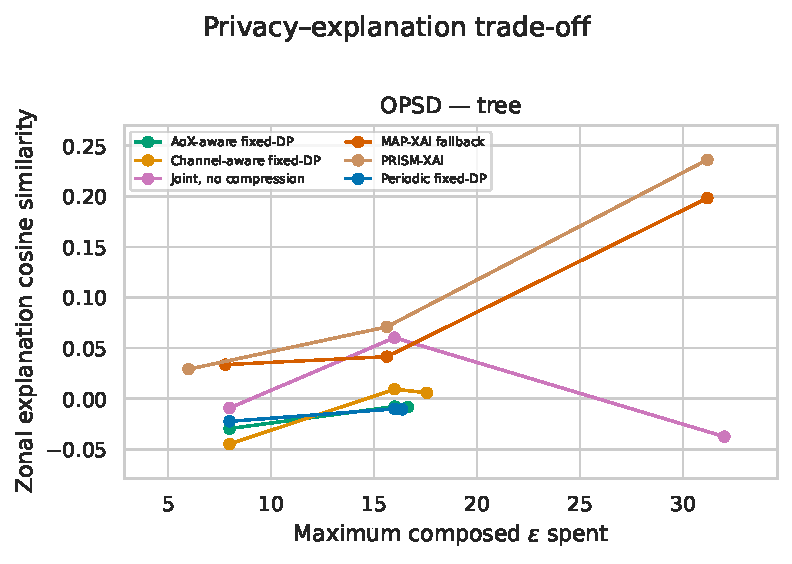
\includegraphics[width=.96\textwidth,height=.82\textheight,keepaspectratio]{../../SERVICE_TRADEOFF_RESULTS/runs/thr_3_cap_16/opsd/privacy_fidelity.pdf}

\caption{Public-score threshold $\tau=3$, release cap $M=16$, OPSD: privacy--fidelity plane. This panel should be read with the setting-level quantitative interpretation and the complete tables immediately preceding the figure block.}

\end{figure*}

\clearpage

\begin{figure*}[p]

\centering

\includegraphics[width=.96\textwidth,height=.82\textheight,keepaspectratio]{../../SERVICE_TRADEOFF_RESULTS/runs/thr_3_cap_16/opsd/pareto_bits_fidelity.pdf}

\caption{Public-score threshold $\tau=3$, release cap $M=16$, OPSD: traffic--fidelity Pareto plane. This panel should be read with the setting-level quantitative interpretation and the complete tables immediately preceding the figure block.}

\end{figure*}

\clearpage

\begin{figure*}[p]

\centering

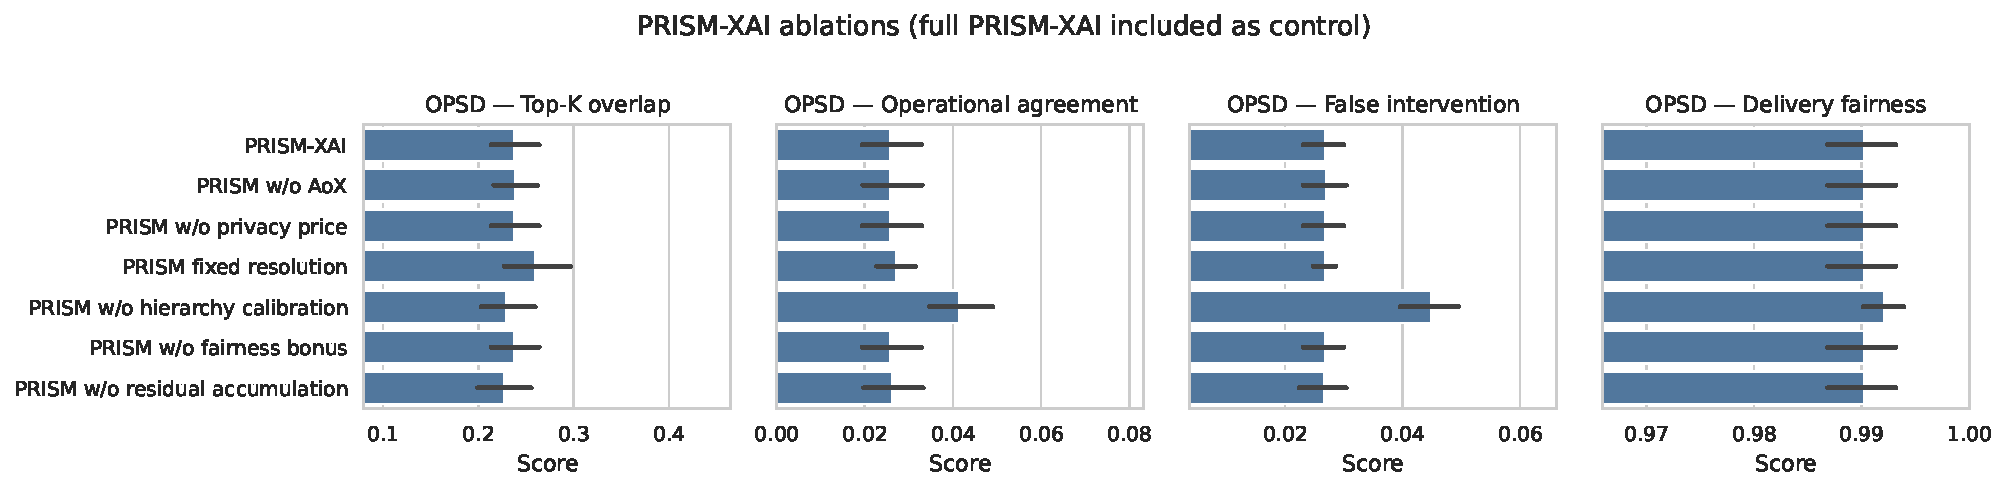
\includegraphics[width=.96\textwidth,height=.82\textheight,keepaspectratio]{../../SERVICE_TRADEOFF_RESULTS/runs/thr_3_cap_16/opsd/ablation_results.pdf}

\caption{Public-score threshold $\tau=3$, release cap $M=16$, OPSD: component ablation. This panel should be read with the setting-level quantitative interpretation and the complete tables immediately preceding the figure block.}

\end{figure*}

\clearpage

\paragraph{UCI.} The three generated tables below report the full method means, all condition-level values, and paired differences. The five figures that follow provide the corresponding temporal, fairness, privacy, Pareto, and ablation views. Aggregate panels support the setting-level summary above; dataset panels reveal whether that summary is shared by OPSD and UCI rather than being driven by their different endpoint counts.

\begin{table*}[p]\centering\tiny

\caption{Public-score threshold $\tau=3$, release cap $M=16$, UCI: complete generated method table.}

\label{tab:thr_3_cap_16:uci:main}

\resizebox{\linewidth}{!}{% Values are means with 95% Student-t confidence intervals across seeds.
\begin{tabular}{lccccccccccccccc}
\toprule
Dataset & Model & $\epsilon_{\max}$ & Method & Top-$K$ & Cosine & Decision & Recall & Prec. & Abst. & P95 ms & kbit & Spent $\epsilon$ & False int. & bit/correct & Fairness \\
\midrule
UCI & Tree & 8 & AoX-aware fixed-DP & 0.263 $\pm$ 0.041 & -0.007 $\pm$ 0.009 & 0.457 $\pm$ 0.031 & 0.457 $\pm$ 0.031 & 0.362 $\pm$ 0.024 & 0.003 $\pm$ 0.001 & 7.500 $\pm$ 0.000 & 5300.224 $\pm$ 0.000 & 7.990 $\pm$ 0.000 & 0.557 $\pm$ 0.025 & 14002.896 $\pm$ 1040.243 & 0.999 $\pm$ 0.000 \\
UCI & Tree & 8 & AoX-aware fixed-DP & 0.260 $\pm$ 0.022 & 0.010 $\pm$ 0.055 & 0.455 $\pm$ 0.047 & 0.455 $\pm$ 0.047 & 0.361 $\pm$ 0.038 & 0.003 $\pm$ 0.001 & 7.500 $\pm$ 0.000 & 5300.224 $\pm$ 0.000 & 7.990 $\pm$ 0.000 & 0.557 $\pm$ 0.048 & 14198.303 $\pm$ 1508.274 & 0.999 $\pm$ 0.000 \\
UCI & Tree & 8 & Channel-aware fixed-DP & 0.248 $\pm$ 0.031 & 0.004 $\pm$ 0.012 & 0.001 $\pm$ 0.001 & 0.001 $\pm$ 0.001 & 0.150 $\pm$ 0.151 & 0.999 $\pm$ 0.001 & 4.609 $\pm$ 1.781 & 5295.177 $\pm$ 3.740 & 7.990 $\pm$ 0.000 & 0.001 $\pm$ 0.001 & 4632196.500 $\pm$ 2102650.252 & 0.991 $\pm$ 0.001 \\
UCI & Tree & 8 & Channel-aware fixed-DP & 0.239 $\pm$ 0.030 & -0.020 $\pm$ 0.055 & 0.000 $\pm$ 0.000 & 0.000 $\pm$ 0.000 & 0.117 $\pm$ 0.225 & 0.999 $\pm$ 0.001 & 4.609 $\pm$ 1.781 & 5295.177 $\pm$ 3.740 & 7.990 $\pm$ 0.000 & 0.001 $\pm$ 0.001 & 5296989.000 $\pm$ 41104.572 & 0.991 $\pm$ 0.001 \\
UCI & Tree & 8 & Joint, no compression & 0.286 $\pm$ 0.045 & 0.004 $\pm$ 0.020 & 0.052 $\pm$ 0.005 & 0.052 $\pm$ 0.005 & 0.406 $\pm$ 0.037 & 0.875 $\pm$ 0.003 & 5.123 $\pm$ 1.792 & 672.300 $\pm$ 0.452 & 7.990 $\pm$ 0.000 & 0.053 $\pm$ 0.004 & 15676.175 $\pm$ 1475.621 & 0.994 $\pm$ 0.003 \\
UCI & Tree & 8 & Joint, no compression & 0.229 $\pm$ 0.052 & -0.032 $\pm$ 0.050 & 0.057 $\pm$ 0.007 & 0.057 $\pm$ 0.007 & 0.428 $\pm$ 0.041 & 0.875 $\pm$ 0.003 & 5.131 $\pm$ 1.787 & 672.300 $\pm$ 0.452 & 7.990 $\pm$ 0.000 & 0.052 $\pm$ 0.004 & 14702.786 $\pm$ 2334.488 & 0.994 $\pm$ 0.003 \\
UCI & Tree & 8 & Periodic fixed-DP & 0.259 $\pm$ 0.060 & -0.005 $\pm$ 0.008 & 0.006 $\pm$ 0.001 & 0.006 $\pm$ 0.001 & 0.244 $\pm$ 0.049 & 0.989 $\pm$ 0.001 & 4.596 $\pm$ 1.788 & 5299.318 $\pm$ 1.451 & 7.786 $\pm$ 0.000 & 0.013 $\pm$ 0.002 & 1215103.896 $\pm$ 390671.319 & 0.999 $\pm$ 0.000 \\
UCI & Tree & 8 & Periodic fixed-DP & 0.260 $\pm$ 0.044 & 0.022 $\pm$ 0.070 & 0.005 $\pm$ 0.001 & 0.005 $\pm$ 0.001 & 0.195 $\pm$ 0.050 & 0.989 $\pm$ 0.001 & 4.596 $\pm$ 1.788 & 5299.318 $\pm$ 1.451 & 7.786 $\pm$ 0.000 & 0.015 $\pm$ 0.002 & 1555837.203 $\pm$ 955472.503 & 0.999 $\pm$ 0.000 \\
UCI & Tree & 8 & PRISM-XAI & 0.231 $\pm$ 0.061 & -0.001 $\pm$ 0.013 & 0.043 $\pm$ 0.009 & 0.043 $\pm$ 0.009 & 0.466 $\pm$ 0.081 & 0.909 $\pm$ 0.005 & 5.656 $\pm$ 1.725 & 328.663 $\pm$ 1.360 & 7.081 $\pm$ 0.177 & 0.033 $\pm$ 0.005 & 10019.834 $\pm$ 2488.756 & 0.990 $\pm$ 0.003 \\
UCI & Tree & 8 & PRISM-XAI & 0.245 $\pm$ 0.047 & -0.007 $\pm$ 0.082 & 0.045 $\pm$ 0.007 & 0.045 $\pm$ 0.007 & 0.507 $\pm$ 0.071 & 0.910 $\pm$ 0.005 & 5.163 $\pm$ 1.785 & 325.833 $\pm$ 1.364 & 7.052 $\pm$ 0.147 & 0.030 $\pm$ 0.006 & 9029.695 $\pm$ 1367.291 & 0.991 $\pm$ 0.002 \\
UCI & Tree & 8 & MAP-XAI fallback & 0.202 $\pm$ 0.058 & 0.011 $\pm$ 0.012 & 0.041 $\pm$ 0.005 & 0.041 $\pm$ 0.005 & 0.453 $\pm$ 0.045 & 0.909 $\pm$ 0.005 & 5.677 $\pm$ 1.704 & 381.702 $\pm$ 0.092 & 7.786 $\pm$ 0.000 & 0.034 $\pm$ 0.003 & 11391.295 $\pm$ 1487.072 & 0.990 $\pm$ 0.003 \\
UCI & Tree & 8 & MAP-XAI fallback & 0.206 $\pm$ 0.051 & 0.062 $\pm$ 0.058 & 0.048 $\pm$ 0.010 & 0.048 $\pm$ 0.010 & 0.505 $\pm$ 0.102 & 0.910 $\pm$ 0.005 & 4.861 $\pm$ 1.663 & 381.256 $\pm$ 0.293 & 7.786 $\pm$ 0.000 & 0.033 $\pm$ 0.007 & 10444.880 $\pm$ 2673.464 & 0.991 $\pm$ 0.002 \\
\bottomrule
\end{tabular}
}

\end{table*}\clearpage

\begin{table*}[p]\centering\tiny

\caption{Public-score threshold $\tau=3$, release cap $M=16$, UCI: complete condition-level generated table.}

\label{tab:thr_3_cap_16:uci:conditions}

\resizebox{\textwidth}{!}{\begin{tabular}{llllccccccccccc}
\toprule
Dataset & Model & $\epsilon_{\max}$ & Method & kbit & Top-$K$ & Random Top-$K$ & Cosine & Decision & Recall & Precision & Coverage & Abstain & False int. & Spent $\epsilon$ \\
\midrule
UCI & Tree & 8 & Joint, no compression & 672.300 $\pm$ 0.452 & 0.286 $\pm$ 0.045 & 0.250 $\pm$ 0.000 & 0.004 $\pm$ 0.020 & 0.052 $\pm$ 0.005 & 0.052 $\pm$ 0.005 & 0.406 $\pm$ 0.037 & 0.125 $\pm$ 0.003 & 0.875 $\pm$ 0.003 & 0.053 $\pm$ 0.004 & 7.990 $\pm$ 0.000 \\
UCI & Tree & 8 & Joint, no compression & 672.300 $\pm$ 0.452 & 0.229 $\pm$ 0.052 & 0.250 $\pm$ 0.000 & -0.032 $\pm$ 0.050 & 0.057 $\pm$ 0.007 & 0.057 $\pm$ 0.007 & 0.428 $\pm$ 0.041 & 0.125 $\pm$ 0.003 & 0.875 $\pm$ 0.003 & 0.052 $\pm$ 0.004 & 7.990 $\pm$ 0.000 \\
UCI & Tree & 8 & Periodic fixed-DP & 5299.318 $\pm$ 1.451 & 0.259 $\pm$ 0.060 & 0.250 $\pm$ 0.000 & -0.005 $\pm$ 0.008 & 0.006 $\pm$ 0.001 & 0.006 $\pm$ 0.001 & 0.244 $\pm$ 0.049 & 0.011 $\pm$ 0.001 & 0.989 $\pm$ 0.001 & 0.013 $\pm$ 0.002 & 7.786 $\pm$ 0.000 \\
UCI & Tree & 8 & Periodic fixed-DP & 5299.318 $\pm$ 1.451 & 0.260 $\pm$ 0.044 & 0.250 $\pm$ 0.000 & 0.022 $\pm$ 0.070 & 0.005 $\pm$ 0.001 & 0.005 $\pm$ 0.001 & 0.195 $\pm$ 0.050 & 0.011 $\pm$ 0.001 & 0.989 $\pm$ 0.001 & 0.015 $\pm$ 0.002 & 7.786 $\pm$ 0.000 \\
UCI & Tree & 8 & PRISM-XAI & 328.663 $\pm$ 1.360 & 0.231 $\pm$ 0.061 & 0.250 $\pm$ 0.000 & -0.001 $\pm$ 0.013 & 0.043 $\pm$ 0.009 & 0.043 $\pm$ 0.009 & 0.466 $\pm$ 0.081 & 0.091 $\pm$ 0.005 & 0.909 $\pm$ 0.005 & 0.033 $\pm$ 0.005 & 7.081 $\pm$ 0.177 \\
UCI & Tree & 8 & PRISM-XAI & 325.833 $\pm$ 1.364 & 0.245 $\pm$ 0.047 & 0.250 $\pm$ 0.000 & -0.007 $\pm$ 0.082 & 0.045 $\pm$ 0.007 & 0.045 $\pm$ 0.007 & 0.507 $\pm$ 0.071 & 0.090 $\pm$ 0.005 & 0.910 $\pm$ 0.005 & 0.030 $\pm$ 0.006 & 7.052 $\pm$ 0.147 \\
UCI & Tree & 16 & Joint, no compression & 1632.150 $\pm$ 0.339 & 0.216 $\pm$ 0.041 & 0.250 $\pm$ 0.000 & 0.001 $\pm$ 0.012 & 0.094 $\pm$ 0.005 & 0.094 $\pm$ 0.005 & 0.330 $\pm$ 0.024 & 0.228 $\pm$ 0.005 & 0.772 $\pm$ 0.005 & 0.133 $\pm$ 0.010 & 15.997 $\pm$ 0.000 \\
UCI & Tree & 16 & Joint, no compression & 1632.600 $\pm$ 0.554 & 0.204 $\pm$ 0.011 & 0.250 $\pm$ 0.000 & -0.021 $\pm$ 0.033 & 0.099 $\pm$ 0.016 & 0.099 $\pm$ 0.016 & 0.347 $\pm$ 0.054 & 0.228 $\pm$ 0.005 & 0.772 $\pm$ 0.005 & 0.128 $\pm$ 0.011 & 15.997 $\pm$ 0.000 \\
UCI & Tree & 16 & Periodic fixed-DP & 5299.318 $\pm$ 1.451 & 0.259 $\pm$ 0.060 & 0.250 $\pm$ 0.000 & -0.005 $\pm$ 0.008 & 0.006 $\pm$ 0.001 & 0.006 $\pm$ 0.001 & 0.244 $\pm$ 0.049 & 0.011 $\pm$ 0.001 & 0.989 $\pm$ 0.001 & 0.013 $\pm$ 0.002 & 7.786 $\pm$ 0.000 \\
UCI & Tree & 16 & Periodic fixed-DP & 5299.318 $\pm$ 1.451 & 0.260 $\pm$ 0.044 & 0.250 $\pm$ 0.000 & 0.022 $\pm$ 0.070 & 0.005 $\pm$ 0.001 & 0.005 $\pm$ 0.001 & 0.195 $\pm$ 0.050 & 0.011 $\pm$ 0.001 & 0.989 $\pm$ 0.001 & 0.015 $\pm$ 0.002 & 7.786 $\pm$ 0.000 \\
UCI & Tree & 16 & PRISM-XAI & 656.329 $\pm$ 1.493 & 0.313 $\pm$ 0.040 & 0.250 $\pm$ 0.000 & 0.015 $\pm$ 0.023 & 0.081 $\pm$ 0.007 & 0.081 $\pm$ 0.007 & 0.445 $\pm$ 0.042 & 0.183 $\pm$ 0.005 & 0.817 $\pm$ 0.005 & 0.070 $\pm$ 0.007 & 15.620 $\pm$ 0.000 \\
UCI & Tree & 16 & PRISM-XAI & 648.965 $\pm$ 1.563 & 0.238 $\pm$ 0.050 & 0.250 $\pm$ 0.000 & -0.027 $\pm$ 0.047 & 0.082 $\pm$ 0.013 & 0.082 $\pm$ 0.013 & 0.471 $\pm$ 0.071 & 0.182 $\pm$ 0.004 & 0.818 $\pm$ 0.004 & 0.064 $\pm$ 0.010 & 15.620 $\pm$ 0.000 \\
UCI & Tree & 32 & Joint, no compression & 4034.550 $\pm$ 5.034 & 0.246 $\pm$ 0.031 & 0.250 $\pm$ 0.000 & -0.002 $\pm$ 0.015 & 0.228 $\pm$ 0.013 & 0.228 $\pm$ 0.013 & 0.361 $\pm$ 0.028 & 0.537 $\pm$ 0.009 & 0.463 $\pm$ 0.009 & 0.279 $\pm$ 0.017 & 31.999 $\pm$ 0.000 \\
UCI & Tree & 32 & Joint, no compression & 4034.550 $\pm$ 5.034 & 0.241 $\pm$ 0.033 & 0.250 $\pm$ 0.000 & -0.012 $\pm$ 0.030 & 0.228 $\pm$ 0.028 & 0.228 $\pm$ 0.028 & 0.360 $\pm$ 0.047 & 0.530 $\pm$ 0.010 & 0.470 $\pm$ 0.010 & 0.280 $\pm$ 0.026 & 31.999 $\pm$ 0.000 \\
UCI & Tree & 32 & Periodic fixed-DP & 5299.318 $\pm$ 1.451 & 0.259 $\pm$ 0.060 & 0.250 $\pm$ 0.000 & -0.005 $\pm$ 0.008 & 0.006 $\pm$ 0.001 & 0.006 $\pm$ 0.001 & 0.244 $\pm$ 0.049 & 0.011 $\pm$ 0.001 & 0.989 $\pm$ 0.001 & 0.013 $\pm$ 0.002 & 7.786 $\pm$ 0.000 \\
UCI & Tree & 32 & Periodic fixed-DP & 5299.318 $\pm$ 1.451 & 0.260 $\pm$ 0.044 & 0.250 $\pm$ 0.000 & 0.022 $\pm$ 0.070 & 0.005 $\pm$ 0.001 & 0.005 $\pm$ 0.001 & 0.195 $\pm$ 0.050 & 0.011 $\pm$ 0.001 & 0.989 $\pm$ 0.001 & 0.015 $\pm$ 0.002 & 7.786 $\pm$ 0.000 \\
UCI & Tree & 32 & PRISM-XAI & 654.773 $\pm$ 1.193 & 0.343 $\pm$ 0.070 & 0.250 $\pm$ 0.000 & 0.019 $\pm$ 0.021 & 0.085 $\pm$ 0.008 & 0.085 $\pm$ 0.008 & 0.556 $\pm$ 0.045 & 0.181 $\pm$ 0.003 & 0.819 $\pm$ 0.003 & 0.048 $\pm$ 0.007 & 31.175 $\pm$ 0.000 \\
UCI & Tree & 32 & PRISM-XAI & 648.024 $\pm$ 1.912 & 0.281 $\pm$ 0.061 & 0.250 $\pm$ 0.000 & -0.049 $\pm$ 0.057 & 0.092 $\pm$ 0.010 & 0.092 $\pm$ 0.010 & 0.595 $\pm$ 0.069 & 0.176 $\pm$ 0.005 & 0.824 $\pm$ 0.005 & 0.044 $\pm$ 0.009 & 31.175 $\pm$ 0.000 \\
\bottomrule
\end{tabular}
}

\end{table*}\clearpage

\begin{table*}[p]\centering\tiny

\caption{Public-score threshold $\tau=3$, release cap $M=16$, UCI: complete generated paired comparisons.}

\label{tab:thr_3_cap_16:uci:paired}

\resizebox{\textwidth}{!}{\begin{tabular}{llcccc}
\toprule
Dataset & Baseline & Delta kbit & Delta Top-$K$ & Delta recall & Delta fairness \\
\midrule
UCI & AoX-aware fixed-DP & -4971.561 $\pm$ 1.360 & -0.033 $\pm$ 0.085 & -0.414 $\pm$ 0.028 & -0.009 $\pm$ 0.003 \\
UCI & AoX-aware fixed-DP & -4643.895 $\pm$ 1.493 & 0.049 $\pm$ 0.050 & -0.376 $\pm$ 0.029 & -0.003 $\pm$ 0.001 \\
UCI & AoX-aware fixed-DP & -4645.451 $\pm$ 1.193 & 0.079 $\pm$ 0.059 & -0.372 $\pm$ 0.030 & -0.003 $\pm$ 0.001 \\
UCI & AoX-aware fixed-DP & -4974.391 $\pm$ 1.364 & -0.016 $\pm$ 0.045 & -0.410 $\pm$ 0.049 & -0.008 $\pm$ 0.002 \\
UCI & AoX-aware fixed-DP & -4651.259 $\pm$ 1.563 & -0.023 $\pm$ 0.046 & -0.372 $\pm$ 0.044 & -0.003 $\pm$ 0.001 \\
UCI & AoX-aware fixed-DP & -4652.200 $\pm$ 1.912 & 0.020 $\pm$ 0.052 & -0.362 $\pm$ 0.051 & -0.003 $\pm$ 0.001 \\
UCI & Channel-aware fixed-DP & -4966.514 $\pm$ 3.919 & -0.018 $\pm$ 0.079 & 0.042 $\pm$ 0.009 & -0.000 $\pm$ 0.002 \\
UCI & Channel-aware fixed-DP & -4643.895 $\pm$ 1.493 & 0.045 $\pm$ 0.059 & 0.080 $\pm$ 0.007 & 0.665 $\pm$ 0.001 \\
UCI & Channel-aware fixed-DP & -4645.451 $\pm$ 1.193 & 0.074 $\pm$ 0.071 & 0.085 $\pm$ 0.009 & 0.741 $\pm$ 0.001 \\
UCI & Channel-aware fixed-DP & -4969.344 $\pm$ 4.185 & 0.006 $\pm$ 0.055 & 0.045 $\pm$ 0.007 & 0.000 $\pm$ 0.002 \\
UCI & Channel-aware fixed-DP & -4651.259 $\pm$ 1.563 & -0.022 $\pm$ 0.058 & 0.082 $\pm$ 0.013 & 0.666 $\pm$ 0.001 \\
UCI & Channel-aware fixed-DP & -4652.200 $\pm$ 1.912 & 0.021 $\pm$ 0.068 & 0.092 $\pm$ 0.011 & 0.741 $\pm$ 0.001 \\
UCI & Joint, no compression & -343.637 $\pm$ 1.641 & -0.055 $\pm$ 0.093 & -0.009 $\pm$ 0.010 & -0.003 $\pm$ 0.003 \\
UCI & Joint, no compression & -975.821 $\pm$ 1.564 & 0.096 $\pm$ 0.035 & -0.013 $\pm$ 0.007 & -0.002 $\pm$ 0.001 \\
UCI & Joint, no compression & -3379.777 $\pm$ 5.671 & 0.097 $\pm$ 0.081 & -0.142 $\pm$ 0.012 & -0.003 $\pm$ 0.001 \\
UCI & Joint, no compression & -346.467 $\pm$ 1.610 & 0.015 $\pm$ 0.070 & -0.012 $\pm$ 0.010 & -0.003 $\pm$ 0.003 \\
UCI & Joint, no compression & -983.635 $\pm$ 1.427 & 0.034 $\pm$ 0.053 & -0.017 $\pm$ 0.024 & -0.002 $\pm$ 0.001 \\
UCI & Joint, no compression & -3386.526 $\pm$ 6.147 & 0.040 $\pm$ 0.071 & -0.135 $\pm$ 0.029 & -0.003 $\pm$ 0.001 \\
UCI & Periodic fixed-DP & -4970.655 $\pm$ 1.984 & -0.029 $\pm$ 0.088 & 0.037 $\pm$ 0.010 & -0.009 $\pm$ 0.003 \\
UCI & Periodic fixed-DP & -4642.989 $\pm$ 2.460 & 0.053 $\pm$ 0.059 & 0.075 $\pm$ 0.007 & -0.003 $\pm$ 0.001 \\
UCI & Periodic fixed-DP & -4644.545 $\pm$ 2.331 & 0.083 $\pm$ 0.082 & 0.080 $\pm$ 0.008 & -0.003 $\pm$ 0.001 \\
UCI & Periodic fixed-DP & -4973.485 $\pm$ 1.727 & -0.016 $\pm$ 0.075 & 0.040 $\pm$ 0.006 & -0.008 $\pm$ 0.002 \\
UCI & Periodic fixed-DP & -4650.353 $\pm$ 1.894 & -0.022 $\pm$ 0.038 & 0.077 $\pm$ 0.012 & -0.003 $\pm$ 0.001 \\
UCI & Periodic fixed-DP & -4651.295 $\pm$ 2.358 & 0.020 $\pm$ 0.078 & 0.087 $\pm$ 0.009 & -0.003 $\pm$ 0.001 \\
UCI & MAP-XAI fallback & -53.039 $\pm$ 1.350 & 0.029 $\pm$ 0.074 & 0.002 $\pm$ 0.006 & 0.000 $\pm$ 0.000 \\
UCI & MAP-XAI fallback & -109.291 $\pm$ 1.508 & 0.053 $\pm$ 0.050 & -0.000 $\pm$ 0.005 & 0.000 $\pm$ 0.000 \\
UCI & MAP-XAI fallback & -110.785 $\pm$ 1.251 & 0.052 $\pm$ 0.090 & 0.001 $\pm$ 0.009 & 0.000 $\pm$ 0.000 \\
UCI & MAP-XAI fallback & -55.422 $\pm$ 1.449 & 0.039 $\pm$ 0.039 & -0.003 $\pm$ 0.007 & 0.000 $\pm$ 0.000 \\
UCI & MAP-XAI fallback & -116.127 $\pm$ 1.715 & 0.008 $\pm$ 0.046 & -0.002 $\pm$ 0.009 & 0.000 $\pm$ 0.000 \\
UCI & MAP-XAI fallback & -116.946 $\pm$ 2.015 & 0.012 $\pm$ 0.040 & 0.014 $\pm$ 0.012 & -0.000 $\pm$ 0.001 \\
\bottomrule
\end{tabular}
}

\end{table*}\clearpage

\begin{figure*}[p]

\centering

\includegraphics[width=.96\textwidth,height=.82\textheight,keepaspectratio]{../../SERVICE_TRADEOFF_RESULTS/runs/thr_3_cap_16/uci/regime_trace.pdf}

\caption{Public-score threshold $\tau=3$, release cap $M=16$, UCI: representative regime trace. This panel should be read with the setting-level quantitative interpretation and the complete tables immediately preceding the figure block.}

\end{figure*}

\clearpage

\begin{figure*}[p]

\centering

\includegraphics[width=.96\textwidth,height=.82\textheight,keepaspectratio]{../../SERVICE_TRADEOFF_RESULTS/runs/thr_3_cap_16/uci/fairness_reliability.pdf}

\caption{Public-score threshold $\tau=3$, release cap $M=16$, UCI: fairness--reliability plane. This panel should be read with the setting-level quantitative interpretation and the complete tables immediately preceding the figure block.}

\end{figure*}

\clearpage

\begin{figure*}[p]

\centering

\includegraphics[width=.96\textwidth,height=.82\textheight,keepaspectratio]{../../SERVICE_TRADEOFF_RESULTS/runs/thr_3_cap_16/uci/privacy_fidelity.pdf}

\caption{Public-score threshold $\tau=3$, release cap $M=16$, UCI: privacy--fidelity plane. This panel should be read with the setting-level quantitative interpretation and the complete tables immediately preceding the figure block.}

\end{figure*}

\clearpage

\begin{figure*}[p]

\centering

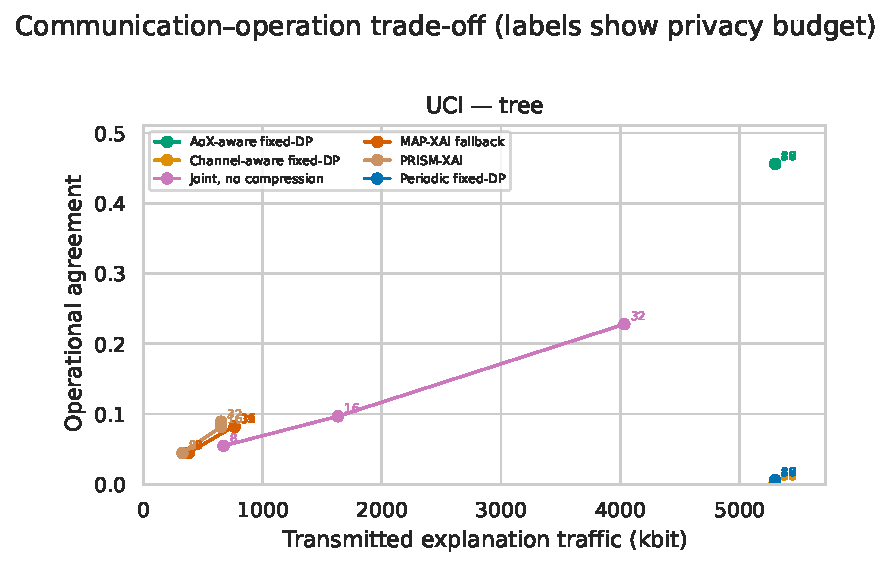
\includegraphics[width=.96\textwidth,height=.82\textheight,keepaspectratio]{../../SERVICE_TRADEOFF_RESULTS/runs/thr_3_cap_16/uci/pareto_bits_fidelity.pdf}

\caption{Public-score threshold $\tau=3$, release cap $M=16$, UCI: traffic--fidelity Pareto plane. This panel should be read with the setting-level quantitative interpretation and the complete tables immediately preceding the figure block.}

\end{figure*}

\clearpage

\begin{figure*}[p]

\centering

\includegraphics[width=.96\textwidth,height=.82\textheight,keepaspectratio]{../../SERVICE_TRADEOFF_RESULTS/runs/thr_3_cap_16/uci/ablation_results.pdf}

\caption{Public-score threshold $\tau=3$, release cap $M=16$, UCI: component ablation. This panel should be read with the setting-level quantitative interpretation and the complete tables immediately preceding the figure block.}

\end{figure*}

\clearpage

\subsubsection{Public-score threshold $\tau=1$, release cap $M=32$}

At this operating point, PRISM-XAI transmits 574.63~kbit versus 688.64~kbit for MAP-XAI-only (aggregate-mean ratio saving 16.56\%). The paired difference is -114.01$\pm$15.13~kbit. PRISM coverage is 0.1402, critical-event recall is 0.0638, and maximum recorded expenditure is 17.196. Relative to MAP-XAI-only, the paired coverage change is -0.00060$\pm$0.00111 and recall change is +0.00153$\pm$0.00178. The descriptive overlap rule holds in 4 of 12 cells. Accordingly, this point is read as a sensitivity point on the service frontier, not a complete matched-service confirmation.

\paragraph{Combined datasets.} The three generated tables below report the full method means, all condition-level values, and paired differences. The five figures that follow provide the corresponding temporal, fairness, privacy, Pareto, and ablation views. Aggregate panels support the setting-level summary above; dataset panels reveal whether that summary is shared by OPSD and UCI rather than being driven by their different endpoint counts.

\begin{table*}[p]\centering\tiny

\caption{Public-score threshold $\tau=1$, release cap $M=32$, Combined datasets: complete generated method table.}

\label{tab:thr_1_cap_32:combined:main}

\resizebox{\linewidth}{!}{% Values are means with 95% Student-t confidence intervals across seeds.
\begin{tabular}{lccccccccccccccc}
\toprule
Dataset & Model & $\epsilon_{\max}$ & Method & Top-$K$ & Cosine & Decision & Recall & Prec. & Abst. & P95 ms & kbit & Spent $\epsilon$ & False int. & bit/correct & Fairness \\
\midrule
OPSD & Tree & 8 & AoX-aware fixed-DP & 0.234 $\pm$ 0.048 & -0.033 $\pm$ 0.028 & 0.119 $\pm$ 0.028 & 0.119 $\pm$ 0.028 & 0.198 $\pm$ 0.054 & 0.721 $\pm$ 0.005 & 6.903 $\pm$ 1.126 & 1560.564 $\pm$ 0.000 & 7.990 $\pm$ 0.000 & 0.183 $\pm$ 0.020 & 35567.482 $\pm$ 10569.818 & 0.999 $\pm$ 0.000 \\
OPSD & Tree & 8 & AoX-aware fixed-DP & 0.238 $\pm$ 0.049 & -0.026 $\pm$ 0.055 & 0.121 $\pm$ 0.026 & 0.121 $\pm$ 0.026 & 0.205 $\pm$ 0.053 & 0.721 $\pm$ 0.005 & 6.903 $\pm$ 1.126 & 1560.564 $\pm$ 0.000 & 7.990 $\pm$ 0.000 & 0.179 $\pm$ 0.023 & 34123.214 $\pm$ 8376.542 & 0.999 $\pm$ 0.000 \\
OPSD & Tree & 8 & Channel-aware fixed-DP & 0.292 $\pm$ 0.037 & -0.041 $\pm$ 0.051 & 0.107 $\pm$ 0.026 & 0.107 $\pm$ 0.026 & 0.217 $\pm$ 0.068 & 0.779 $\pm$ 0.011 & 5.571 $\pm$ 1.784 & 1560.564 $\pm$ 0.000 & 7.990 $\pm$ 0.000 & 0.154 $\pm$ 0.029 & 40860.756 $\pm$ 14126.920 & 0.999 $\pm$ 0.000 \\
OPSD & Tree & 8 & Channel-aware fixed-DP & 0.292 $\pm$ 0.054 & -0.049 $\pm$ 0.064 & 0.111 $\pm$ 0.023 & 0.111 $\pm$ 0.023 & 0.228 $\pm$ 0.066 & 0.779 $\pm$ 0.011 & 5.571 $\pm$ 1.784 & 1560.564 $\pm$ 0.000 & 7.990 $\pm$ 0.000 & 0.149 $\pm$ 0.026 & 37980.855 $\pm$ 12338.094 & 0.999 $\pm$ 0.000 \\
OPSD & Tree & 8 & Joint, no compression & 0.288 $\pm$ 0.064 & -0.030 $\pm$ 0.079 & 0.016 $\pm$ 0.005 & 0.016 $\pm$ 0.005 & 0.193 $\pm$ 0.059 & 0.957 $\pm$ 0.003 & 4.560 $\pm$ 1.811 & 189.900 $\pm$ 0.554 & 7.990 $\pm$ 0.000 & 0.027 $\pm$ 0.005 & 32490.357 $\pm$ 10149.755 & 0.996 $\pm$ 0.002 \\
OPSD & Tree & 8 & Joint, no compression & 0.258 $\pm$ 0.055 & 0.011 $\pm$ 0.094 & 0.019 $\pm$ 0.004 & 0.019 $\pm$ 0.004 & 0.224 $\pm$ 0.044 & 0.957 $\pm$ 0.003 & 4.562 $\pm$ 1.809 & 189.750 $\pm$ 0.566 & 7.990 $\pm$ 0.000 & 0.025 $\pm$ 0.003 & 26079.167 $\pm$ 6335.386 & 0.996 $\pm$ 0.002 \\
OPSD & Tree & 8 & Periodic fixed-DP & 0.241 $\pm$ 0.049 & -0.019 $\pm$ 0.061 & 0.125 $\pm$ 0.020 & 0.125 $\pm$ 0.020 & 0.209 $\pm$ 0.044 & 0.722 $\pm$ 0.006 & 6.303 $\pm$ 1.438 & 1560.564 $\pm$ 0.000 & 7.990 $\pm$ 0.000 & 0.181 $\pm$ 0.021 & 31183.082 $\pm$ 4356.378 & 0.999 $\pm$ 0.000 \\
OPSD & Tree & 8 & Periodic fixed-DP & 0.242 $\pm$ 0.048 & -0.026 $\pm$ 0.082 & 0.135 $\pm$ 0.016 & 0.135 $\pm$ 0.016 & 0.231 $\pm$ 0.037 & 0.722 $\pm$ 0.006 & 6.303 $\pm$ 1.438 & 1560.564 $\pm$ 0.000 & 7.990 $\pm$ 0.000 & 0.169 $\pm$ 0.017 & 28520.235 $\pm$ 3511.595 & 0.999 $\pm$ 0.000 \\
OPSD & Tree & 8 & PRISM-XAI & 0.261 $\pm$ 0.053 & -0.019 $\pm$ 0.080 & 0.021 $\pm$ 0.005 & 0.021 $\pm$ 0.005 & 0.246 $\pm$ 0.094 & 0.947 $\pm$ 0.003 & 4.452 $\pm$ 1.878 & 97.640 $\pm$ 0.539 & 5.377 $\pm$ 0.416 & 0.027 $\pm$ 0.007 & 13250.048 $\pm$ 5126.243 & 0.994 $\pm$ 0.003 \\
OPSD & Tree & 8 & PRISM-XAI & 0.284 $\pm$ 0.064 & -0.006 $\pm$ 0.076 & 0.022 $\pm$ 0.005 & 0.022 $\pm$ 0.005 & 0.253 $\pm$ 0.080 & 0.947 $\pm$ 0.003 & 4.452 $\pm$ 1.878 & 97.251 $\pm$ 0.416 & 5.108 $\pm$ 0.367 & 0.026 $\pm$ 0.006 & 12180.416 $\pm$ 3594.328 & 0.994 $\pm$ 0.003 \\
OPSD & Tree & 8 & MAP-XAI fallback & 0.249 $\pm$ 0.062 & -0.025 $\pm$ 0.053 & 0.019 $\pm$ 0.007 & 0.019 $\pm$ 0.007 & 0.212 $\pm$ 0.098 & 0.947 $\pm$ 0.003 & 4.568 $\pm$ 1.808 & 117.817 $\pm$ 0.049 & 7.924 $\pm$ 0.000 & 0.030 $\pm$ 0.007 & 25854.893 $\pm$ 23642.714 & 0.994 $\pm$ 0.003 \\
OPSD & Tree & 8 & MAP-XAI fallback & 0.233 $\pm$ 0.051 & 0.005 $\pm$ 0.068 & 0.022 $\pm$ 0.007 & 0.022 $\pm$ 0.007 & 0.257 $\pm$ 0.098 & 0.947 $\pm$ 0.003 & 4.568 $\pm$ 1.808 & 117.675 $\pm$ 0.049 & 7.924 $\pm$ 0.000 & 0.026 $\pm$ 0.007 & 18081.688 $\pm$ 11158.136 & 0.994 $\pm$ 0.003 \\
UCI & Tree & 8 & AoX-aware fixed-DP & 0.263 $\pm$ 0.041 & -0.007 $\pm$ 0.009 & 0.457 $\pm$ 0.031 & 0.457 $\pm$ 0.031 & 0.362 $\pm$ 0.024 & 0.003 $\pm$ 0.001 & 7.500 $\pm$ 0.000 & 5300.224 $\pm$ 0.000 & 7.990 $\pm$ 0.000 & 0.557 $\pm$ 0.025 & 14002.896 $\pm$ 1040.243 & 0.999 $\pm$ 0.000 \\
UCI & Tree & 8 & AoX-aware fixed-DP & 0.260 $\pm$ 0.022 & 0.010 $\pm$ 0.055 & 0.455 $\pm$ 0.047 & 0.455 $\pm$ 0.047 & 0.361 $\pm$ 0.038 & 0.003 $\pm$ 0.001 & 7.500 $\pm$ 0.000 & 5300.224 $\pm$ 0.000 & 7.990 $\pm$ 0.000 & 0.557 $\pm$ 0.048 & 14198.303 $\pm$ 1508.274 & 0.999 $\pm$ 0.000 \\
UCI & Tree & 8 & Channel-aware fixed-DP & 0.248 $\pm$ 0.031 & 0.004 $\pm$ 0.012 & 0.001 $\pm$ 0.001 & 0.001 $\pm$ 0.001 & 0.150 $\pm$ 0.151 & 0.999 $\pm$ 0.001 & 4.609 $\pm$ 1.781 & 5295.177 $\pm$ 3.740 & 7.990 $\pm$ 0.000 & 0.001 $\pm$ 0.001 & 4632196.500 $\pm$ 2102650.252 & 0.991 $\pm$ 0.001 \\
UCI & Tree & 8 & Channel-aware fixed-DP & 0.239 $\pm$ 0.030 & -0.020 $\pm$ 0.055 & 0.000 $\pm$ 0.000 & 0.000 $\pm$ 0.000 & 0.117 $\pm$ 0.225 & 0.999 $\pm$ 0.001 & 4.609 $\pm$ 1.781 & 5295.177 $\pm$ 3.740 & 7.990 $\pm$ 0.000 & 0.001 $\pm$ 0.001 & 5296989.000 $\pm$ 41104.572 & 0.991 $\pm$ 0.001 \\
UCI & Tree & 8 & Joint, no compression & 0.286 $\pm$ 0.045 & 0.004 $\pm$ 0.020 & 0.052 $\pm$ 0.005 & 0.052 $\pm$ 0.005 & 0.406 $\pm$ 0.037 & 0.875 $\pm$ 0.003 & 5.123 $\pm$ 1.792 & 672.300 $\pm$ 0.452 & 7.990 $\pm$ 0.000 & 0.053 $\pm$ 0.004 & 15676.175 $\pm$ 1475.621 & 0.994 $\pm$ 0.003 \\
UCI & Tree & 8 & Joint, no compression & 0.229 $\pm$ 0.052 & -0.032 $\pm$ 0.050 & 0.057 $\pm$ 0.007 & 0.057 $\pm$ 0.007 & 0.428 $\pm$ 0.041 & 0.875 $\pm$ 0.003 & 5.131 $\pm$ 1.787 & 672.300 $\pm$ 0.452 & 7.990 $\pm$ 0.000 & 0.052 $\pm$ 0.004 & 14702.786 $\pm$ 2334.488 & 0.994 $\pm$ 0.003 \\
UCI & Tree & 8 & Periodic fixed-DP & 0.259 $\pm$ 0.060 & -0.005 $\pm$ 0.008 & 0.006 $\pm$ 0.001 & 0.006 $\pm$ 0.001 & 0.244 $\pm$ 0.049 & 0.989 $\pm$ 0.001 & 4.596 $\pm$ 1.788 & 5299.318 $\pm$ 1.451 & 7.786 $\pm$ 0.000 & 0.013 $\pm$ 0.002 & 1215103.896 $\pm$ 390671.319 & 0.999 $\pm$ 0.000 \\
UCI & Tree & 8 & Periodic fixed-DP & 0.260 $\pm$ 0.044 & 0.022 $\pm$ 0.070 & 0.005 $\pm$ 0.001 & 0.005 $\pm$ 0.001 & 0.195 $\pm$ 0.050 & 0.989 $\pm$ 0.001 & 4.596 $\pm$ 1.788 & 5299.318 $\pm$ 1.451 & 7.786 $\pm$ 0.000 & 0.015 $\pm$ 0.002 & 1555837.203 $\pm$ 955472.503 & 0.999 $\pm$ 0.000 \\
UCI & Tree & 8 & PRISM-XAI & 0.270 $\pm$ 0.078 & -0.004 $\pm$ 0.021 & 0.029 $\pm$ 0.006 & 0.029 $\pm$ 0.006 & 0.346 $\pm$ 0.060 & 0.928 $\pm$ 0.003 & 5.789 $\pm$ 1.601 & 333.552 $\pm$ 0.722 & 6.549 $\pm$ 0.228 & 0.037 $\pm$ 0.005 & 15343.847 $\pm$ 4327.572 & 0.989 $\pm$ 0.003 \\
UCI & Tree & 8 & PRISM-XAI & 0.262 $\pm$ 0.032 & -0.011 $\pm$ 0.061 & 0.031 $\pm$ 0.004 & 0.031 $\pm$ 0.004 & 0.416 $\pm$ 0.078 & 0.931 $\pm$ 0.004 & 4.104 $\pm$ 1.678 & 331.348 $\pm$ 1.358 & 6.250 $\pm$ 0.232 & 0.031 $\pm$ 0.006 & 13176.006 $\pm$ 1853.692 & 0.988 $\pm$ 0.003 \\
UCI & Tree & 8 & MAP-XAI fallback & 0.256 $\pm$ 0.104 & -0.001 $\pm$ 0.023 & 0.030 $\pm$ 0.005 & 0.030 $\pm$ 0.005 & 0.390 $\pm$ 0.058 & 0.929 $\pm$ 0.004 & 5.428 $\pm$ 1.682 & 394.757 $\pm$ 0.724 & 7.924 $\pm$ 0.000 & 0.033 $\pm$ 0.004 & 17064.051 $\pm$ 5665.496 & 0.990 $\pm$ 0.003 \\
UCI & Tree & 8 & MAP-XAI fallback & 0.215 $\pm$ 0.046 & 0.034 $\pm$ 0.038 & 0.031 $\pm$ 0.003 & 0.031 $\pm$ 0.003 & 0.437 $\pm$ 0.060 & 0.932 $\pm$ 0.004 & 5.132 $\pm$ 1.788 & 393.884 $\pm$ 0.595 & 7.924 $\pm$ 0.000 & 0.029 $\pm$ 0.006 & 15461.186 $\pm$ 1718.511 & 0.988 $\pm$ 0.003 \\
\bottomrule
\end{tabular}
}

\end{table*}\clearpage

\begin{table*}[p]\centering\tiny

\caption{Public-score threshold $\tau=1$, release cap $M=32$, Combined datasets: complete condition-level generated table.}

\label{tab:thr_1_cap_32:combined:conditions}

\resizebox{\textwidth}{!}{\begin{tabular}{llllccccccccccc}
\toprule
Dataset & Model & $\epsilon_{\max}$ & Method & kbit & Top-$K$ & Random Top-$K$ & Cosine & Decision & Recall & Precision & Coverage & Abstain & False int. & Spent $\epsilon$ \\
\midrule
OPSD & Tree & 8 & Joint, no compression & 189.900 $\pm$ 0.554 & 0.288 $\pm$ 0.064 & 0.250 $\pm$ 0.000 & -0.030 $\pm$ 0.079 & 0.016 $\pm$ 0.005 & 0.016 $\pm$ 0.005 & 0.193 $\pm$ 0.059 & 0.043 $\pm$ 0.003 & 0.957 $\pm$ 0.003 & 0.027 $\pm$ 0.005 & 7.990 $\pm$ 0.000 \\
OPSD & Tree & 8 & Joint, no compression & 189.750 $\pm$ 0.566 & 0.258 $\pm$ 0.055 & 0.250 $\pm$ 0.000 & 0.011 $\pm$ 0.094 & 0.019 $\pm$ 0.004 & 0.019 $\pm$ 0.004 & 0.224 $\pm$ 0.044 & 0.043 $\pm$ 0.003 & 0.957 $\pm$ 0.003 & 0.025 $\pm$ 0.003 & 7.990 $\pm$ 0.000 \\
OPSD & Tree & 8 & Periodic fixed-DP & 1560.564 $\pm$ 0.000 & 0.241 $\pm$ 0.049 & 0.250 $\pm$ 0.000 & -0.019 $\pm$ 0.061 & 0.125 $\pm$ 0.020 & 0.125 $\pm$ 0.020 & 0.209 $\pm$ 0.044 & 0.278 $\pm$ 0.006 & 0.722 $\pm$ 0.006 & 0.181 $\pm$ 0.021 & 7.990 $\pm$ 0.000 \\
OPSD & Tree & 8 & Periodic fixed-DP & 1560.564 $\pm$ 0.000 & 0.242 $\pm$ 0.048 & 0.250 $\pm$ 0.000 & -0.026 $\pm$ 0.082 & 0.135 $\pm$ 0.016 & 0.135 $\pm$ 0.016 & 0.231 $\pm$ 0.037 & 0.278 $\pm$ 0.006 & 0.722 $\pm$ 0.006 & 0.169 $\pm$ 0.017 & 7.990 $\pm$ 0.000 \\
OPSD & Tree & 8 & PRISM-XAI & 97.640 $\pm$ 0.539 & 0.261 $\pm$ 0.053 & 0.250 $\pm$ 0.000 & -0.019 $\pm$ 0.080 & 0.021 $\pm$ 0.005 & 0.021 $\pm$ 0.005 & 0.246 $\pm$ 0.094 & 0.053 $\pm$ 0.003 & 0.947 $\pm$ 0.003 & 0.027 $\pm$ 0.007 & 5.377 $\pm$ 0.416 \\
OPSD & Tree & 8 & PRISM-XAI & 97.251 $\pm$ 0.416 & 0.284 $\pm$ 0.064 & 0.250 $\pm$ 0.000 & -0.006 $\pm$ 0.076 & 0.022 $\pm$ 0.005 & 0.022 $\pm$ 0.005 & 0.253 $\pm$ 0.080 & 0.053 $\pm$ 0.003 & 0.947 $\pm$ 0.003 & 0.026 $\pm$ 0.006 & 5.108 $\pm$ 0.367 \\
OPSD & Tree & 16 & Joint, no compression & 459.900 $\pm$ 0.750 & 0.232 $\pm$ 0.065 & 0.250 $\pm$ 0.000 & 0.059 $\pm$ 0.048 & 0.038 $\pm$ 0.009 & 0.038 $\pm$ 0.009 & 0.222 $\pm$ 0.049 & 0.088 $\pm$ 0.004 & 0.912 $\pm$ 0.004 & 0.049 $\pm$ 0.005 & 15.997 $\pm$ 0.000 \\
OPSD & Tree & 16 & Joint, no compression & 460.050 $\pm$ 0.724 & 0.241 $\pm$ 0.055 & 0.250 $\pm$ 0.000 & 0.061 $\pm$ 0.052 & 0.039 $\pm$ 0.008 & 0.039 $\pm$ 0.008 & 0.241 $\pm$ 0.042 & 0.088 $\pm$ 0.004 & 0.912 $\pm$ 0.004 & 0.045 $\pm$ 0.004 & 15.997 $\pm$ 0.000 \\
OPSD & Tree & 16 & Periodic fixed-DP & 5112.594 $\pm$ 0.000 & 0.249 $\pm$ 0.022 & 0.250 $\pm$ 0.000 & -0.009 $\pm$ 0.045 & 0.450 $\pm$ 0.062 & 0.450 $\pm$ 0.062 & 0.237 $\pm$ 0.042 & 0.985 $\pm$ 0.002 & 0.015 $\pm$ 0.002 & 0.551 $\pm$ 0.057 & 15.997 $\pm$ 0.000 \\
OPSD & Tree & 16 & Periodic fixed-DP & 5112.594 $\pm$ 0.000 & 0.243 $\pm$ 0.019 & 0.250 $\pm$ 0.000 & -0.012 $\pm$ 0.050 & 0.463 $\pm$ 0.047 & 0.463 $\pm$ 0.047 & 0.240 $\pm$ 0.028 & 0.985 $\pm$ 0.002 & 0.015 $\pm$ 0.002 & 0.547 $\pm$ 0.036 & 15.997 $\pm$ 0.000 \\
OPSD & Tree & 16 & PRISM-XAI & 296.336 $\pm$ 0.924 & 0.239 $\pm$ 0.051 & 0.250 $\pm$ 0.000 & 0.018 $\pm$ 0.080 & 0.059 $\pm$ 0.016 & 0.059 $\pm$ 0.016 & 0.259 $\pm$ 0.080 & 0.134 $\pm$ 0.004 & 0.866 $\pm$ 0.004 & 0.066 $\pm$ 0.012 & 14.393 $\pm$ 0.046 \\
OPSD & Tree & 16 & PRISM-XAI & 295.240 $\pm$ 0.855 & 0.226 $\pm$ 0.027 & 0.250 $\pm$ 0.000 & 0.001 $\pm$ 0.087 & 0.061 $\pm$ 0.015 & 0.061 $\pm$ 0.015 & 0.274 $\pm$ 0.080 & 0.134 $\pm$ 0.004 & 0.866 $\pm$ 0.004 & 0.065 $\pm$ 0.014 & 14.360 $\pm$ 0.035 \\
OPSD & Tree & 32 & Joint, no compression & 1140.900 $\pm$ 7.953 & 0.235 $\pm$ 0.064 & 0.250 $\pm$ 0.000 & -0.031 $\pm$ 0.089 & 0.074 $\pm$ 0.015 & 0.074 $\pm$ 0.015 & 0.205 $\pm$ 0.039 & 0.157 $\pm$ 0.006 & 0.843 $\pm$ 0.006 & 0.107 $\pm$ 0.009 & 31.999 $\pm$ 0.000 \\
OPSD & Tree & 32 & Joint, no compression & 1140.900 $\pm$ 7.953 & 0.282 $\pm$ 0.054 & 0.250 $\pm$ 0.000 & -0.044 $\pm$ 0.076 & 0.080 $\pm$ 0.011 & 0.080 $\pm$ 0.011 & 0.227 $\pm$ 0.052 & 0.158 $\pm$ 0.006 & 0.842 $\pm$ 0.006 & 0.105 $\pm$ 0.015 & 31.999 $\pm$ 0.000 \\
OPSD & Tree & 32 & Periodic fixed-DP & 5299.836 $\pm$ 0.625 & 0.249 $\pm$ 0.022 & 0.250 $\pm$ 0.000 & -0.009 $\pm$ 0.044 & 0.458 $\pm$ 0.066 & 0.458 $\pm$ 0.066 & 0.237 $\pm$ 0.045 & 1.000 $\pm$ 0.000 & 0.000 $\pm$ 0.000 & 0.562 $\pm$ 0.062 & 16.371 $\pm$ 0.000 \\
OPSD & Tree & 32 & Periodic fixed-DP & 5299.836 $\pm$ 0.625 & 0.244 $\pm$ 0.019 & 0.250 $\pm$ 0.000 & -0.012 $\pm$ 0.050 & 0.471 $\pm$ 0.049 & 0.471 $\pm$ 0.049 & 0.240 $\pm$ 0.029 & 1.000 $\pm$ 0.000 & 0.000 $\pm$ 0.000 & 0.559 $\pm$ 0.039 & 16.371 $\pm$ 0.000 \\
OPSD & Tree & 32 & PRISM-XAI & 350.911 $\pm$ 0.837 & 0.222 $\pm$ 0.050 & 0.250 $\pm$ 0.000 & 0.012 $\pm$ 0.068 & 0.062 $\pm$ 0.017 & 0.062 $\pm$ 0.017 & 0.228 $\pm$ 0.070 & 0.140 $\pm$ 0.005 & 0.860 $\pm$ 0.005 & 0.082 $\pm$ 0.015 & 31.175 $\pm$ 0.000 \\
OPSD & Tree & 32 & PRISM-XAI & 349.693 $\pm$ 0.728 & 0.243 $\pm$ 0.064 & 0.250 $\pm$ 0.000 & 0.019 $\pm$ 0.085 & 0.060 $\pm$ 0.016 & 0.060 $\pm$ 0.016 & 0.233 $\pm$ 0.084 & 0.140 $\pm$ 0.005 & 0.860 $\pm$ 0.005 & 0.081 $\pm$ 0.019 & 31.175 $\pm$ 0.000 \\
UCI & Tree & 8 & Joint, no compression & 672.300 $\pm$ 0.452 & 0.286 $\pm$ 0.045 & 0.250 $\pm$ 0.000 & 0.004 $\pm$ 0.020 & 0.052 $\pm$ 0.005 & 0.052 $\pm$ 0.005 & 0.406 $\pm$ 0.037 & 0.125 $\pm$ 0.003 & 0.875 $\pm$ 0.003 & 0.053 $\pm$ 0.004 & 7.990 $\pm$ 0.000 \\
UCI & Tree & 8 & Joint, no compression & 672.300 $\pm$ 0.452 & 0.229 $\pm$ 0.052 & 0.250 $\pm$ 0.000 & -0.032 $\pm$ 0.050 & 0.057 $\pm$ 0.007 & 0.057 $\pm$ 0.007 & 0.428 $\pm$ 0.041 & 0.125 $\pm$ 0.003 & 0.875 $\pm$ 0.003 & 0.052 $\pm$ 0.004 & 7.990 $\pm$ 0.000 \\
UCI & Tree & 8 & Periodic fixed-DP & 5299.318 $\pm$ 1.451 & 0.259 $\pm$ 0.060 & 0.250 $\pm$ 0.000 & -0.005 $\pm$ 0.008 & 0.006 $\pm$ 0.001 & 0.006 $\pm$ 0.001 & 0.244 $\pm$ 0.049 & 0.011 $\pm$ 0.001 & 0.989 $\pm$ 0.001 & 0.013 $\pm$ 0.002 & 7.786 $\pm$ 0.000 \\
UCI & Tree & 8 & Periodic fixed-DP & 5299.318 $\pm$ 1.451 & 0.260 $\pm$ 0.044 & 0.250 $\pm$ 0.000 & 0.022 $\pm$ 0.070 & 0.005 $\pm$ 0.001 & 0.005 $\pm$ 0.001 & 0.195 $\pm$ 0.050 & 0.011 $\pm$ 0.001 & 0.989 $\pm$ 0.001 & 0.015 $\pm$ 0.002 & 7.786 $\pm$ 0.000 \\
UCI & Tree & 8 & PRISM-XAI & 333.552 $\pm$ 0.722 & 0.270 $\pm$ 0.078 & 0.250 $\pm$ 0.000 & -0.004 $\pm$ 0.021 & 0.029 $\pm$ 0.006 & 0.029 $\pm$ 0.006 & 0.346 $\pm$ 0.060 & 0.072 $\pm$ 0.003 & 0.928 $\pm$ 0.003 & 0.037 $\pm$ 0.005 & 6.549 $\pm$ 0.228 \\
UCI & Tree & 8 & PRISM-XAI & 331.348 $\pm$ 1.358 & 0.262 $\pm$ 0.032 & 0.250 $\pm$ 0.000 & -0.011 $\pm$ 0.061 & 0.031 $\pm$ 0.004 & 0.031 $\pm$ 0.004 & 0.416 $\pm$ 0.078 & 0.069 $\pm$ 0.004 & 0.931 $\pm$ 0.004 & 0.031 $\pm$ 0.006 & 6.250 $\pm$ 0.232 \\
UCI & Tree & 16 & Joint, no compression & 1632.150 $\pm$ 0.339 & 0.216 $\pm$ 0.041 & 0.250 $\pm$ 0.000 & 0.001 $\pm$ 0.012 & 0.094 $\pm$ 0.005 & 0.094 $\pm$ 0.005 & 0.330 $\pm$ 0.024 & 0.228 $\pm$ 0.005 & 0.772 $\pm$ 0.005 & 0.133 $\pm$ 0.010 & 15.997 $\pm$ 0.000 \\
UCI & Tree & 16 & Joint, no compression & 1632.600 $\pm$ 0.554 & 0.204 $\pm$ 0.011 & 0.250 $\pm$ 0.000 & -0.021 $\pm$ 0.033 & 0.099 $\pm$ 0.016 & 0.099 $\pm$ 0.016 & 0.347 $\pm$ 0.054 & 0.228 $\pm$ 0.005 & 0.772 $\pm$ 0.005 & 0.128 $\pm$ 0.011 & 15.997 $\pm$ 0.000 \\
UCI & Tree & 16 & Periodic fixed-DP & 5299.318 $\pm$ 1.451 & 0.259 $\pm$ 0.060 & 0.250 $\pm$ 0.000 & -0.005 $\pm$ 0.008 & 0.006 $\pm$ 0.001 & 0.006 $\pm$ 0.001 & 0.244 $\pm$ 0.049 & 0.011 $\pm$ 0.001 & 0.989 $\pm$ 0.001 & 0.013 $\pm$ 0.002 & 7.786 $\pm$ 0.000 \\
UCI & Tree & 16 & Periodic fixed-DP & 5299.318 $\pm$ 1.451 & 0.260 $\pm$ 0.044 & 0.250 $\pm$ 0.000 & 0.022 $\pm$ 0.070 & 0.005 $\pm$ 0.001 & 0.005 $\pm$ 0.001 & 0.195 $\pm$ 0.050 & 0.011 $\pm$ 0.001 & 0.989 $\pm$ 0.001 & 0.015 $\pm$ 0.002 & 7.786 $\pm$ 0.000 \\
UCI & Tree & 16 & PRISM-XAI & 1088.410 $\pm$ 2.255 & 0.252 $\pm$ 0.062 & 0.250 $\pm$ 0.000 & 0.007 $\pm$ 0.013 & 0.106 $\pm$ 0.014 & 0.106 $\pm$ 0.014 & 0.397 $\pm$ 0.042 & 0.218 $\pm$ 0.007 & 0.782 $\pm$ 0.007 & 0.110 $\pm$ 0.007 & 14.811 $\pm$ 0.029 \\
UCI & Tree & 16 & PRISM-XAI & 1081.416 $\pm$ 2.529 & 0.236 $\pm$ 0.022 & 0.250 $\pm$ 0.000 & 0.006 $\pm$ 0.081 & 0.098 $\pm$ 0.011 & 0.098 $\pm$ 0.011 & 0.394 $\pm$ 0.027 & 0.208 $\pm$ 0.013 & 0.792 $\pm$ 0.013 & 0.104 $\pm$ 0.012 & 14.805 $\pm$ 0.044 \\
UCI & Tree & 32 & Joint, no compression & 4034.550 $\pm$ 5.034 & 0.246 $\pm$ 0.031 & 0.250 $\pm$ 0.000 & -0.002 $\pm$ 0.015 & 0.228 $\pm$ 0.013 & 0.228 $\pm$ 0.013 & 0.361 $\pm$ 0.028 & 0.537 $\pm$ 0.009 & 0.463 $\pm$ 0.009 & 0.279 $\pm$ 0.017 & 31.999 $\pm$ 0.000 \\
UCI & Tree & 32 & Joint, no compression & 4034.550 $\pm$ 5.034 & 0.241 $\pm$ 0.033 & 0.250 $\pm$ 0.000 & -0.012 $\pm$ 0.030 & 0.228 $\pm$ 0.028 & 0.228 $\pm$ 0.028 & 0.360 $\pm$ 0.047 & 0.530 $\pm$ 0.010 & 0.470 $\pm$ 0.010 & 0.280 $\pm$ 0.026 & 31.999 $\pm$ 0.000 \\
UCI & Tree & 32 & Periodic fixed-DP & 5299.318 $\pm$ 1.451 & 0.259 $\pm$ 0.060 & 0.250 $\pm$ 0.000 & -0.005 $\pm$ 0.008 & 0.006 $\pm$ 0.001 & 0.006 $\pm$ 0.001 & 0.244 $\pm$ 0.049 & 0.011 $\pm$ 0.001 & 0.989 $\pm$ 0.001 & 0.013 $\pm$ 0.002 & 7.786 $\pm$ 0.000 \\
UCI & Tree & 32 & Periodic fixed-DP & 5299.318 $\pm$ 1.451 & 0.260 $\pm$ 0.044 & 0.250 $\pm$ 0.000 & 0.022 $\pm$ 0.070 & 0.005 $\pm$ 0.001 & 0.005 $\pm$ 0.001 & 0.195 $\pm$ 0.050 & 0.011 $\pm$ 0.001 & 0.989 $\pm$ 0.001 & 0.015 $\pm$ 0.002 & 7.786 $\pm$ 0.000 \\
UCI & Tree & 32 & PRISM-XAI & 1289.912 $\pm$ 2.162 & 0.259 $\pm$ 0.042 & 0.250 $\pm$ 0.000 & 0.016 $\pm$ 0.015 & 0.118 $\pm$ 0.011 & 0.118 $\pm$ 0.011 & 0.389 $\pm$ 0.026 & 0.247 $\pm$ 0.009 & 0.753 $\pm$ 0.009 & 0.128 $\pm$ 0.011 & 31.175 $\pm$ 0.000 \\
UCI & Tree & 32 & PRISM-XAI & 1283.870 $\pm$ 3.710 & 0.235 $\pm$ 0.035 & 0.250 $\pm$ 0.000 & 0.020 $\pm$ 0.034 & 0.100 $\pm$ 0.015 & 0.100 $\pm$ 0.015 & 0.395 $\pm$ 0.041 & 0.216 $\pm$ 0.019 & 0.784 $\pm$ 0.019 & 0.105 $\pm$ 0.010 & 31.175 $\pm$ 0.000 \\
\bottomrule
\end{tabular}
}

\end{table*}\clearpage

\begin{table*}[p]\centering\tiny

\caption{Public-score threshold $\tau=1$, release cap $M=32$, Combined datasets: complete generated paired comparisons.}

\label{tab:thr_1_cap_32:combined:paired}

\resizebox{\textwidth}{!}{\begin{tabular}{llcccc}
\toprule
Dataset & Baseline & Delta kbit & Delta Top-$K$ & Delta recall & Delta fairness \\
\midrule
OPSD & AoX-aware fixed-DP & -1462.924 $\pm$ 0.539 & 0.027 $\pm$ 0.083 & -0.099 $\pm$ 0.029 & -0.006 $\pm$ 0.003 \\
OPSD & AoX-aware fixed-DP & -4803.577 $\pm$ 5.551 & -0.015 $\pm$ 0.045 & -0.343 $\pm$ 0.075 & -0.003 $\pm$ 0.002 \\
OPSD & AoX-aware fixed-DP & -4949.313 $\pm$ 0.837 & -0.030 $\pm$ 0.066 & -0.350 $\pm$ 0.078 & -0.002 $\pm$ 0.001 \\
OPSD & AoX-aware fixed-DP & -1463.313 $\pm$ 0.416 & 0.046 $\pm$ 0.054 & -0.099 $\pm$ 0.026 & -0.006 $\pm$ 0.003 \\
OPSD & AoX-aware fixed-DP & -4804.672 $\pm$ 5.519 & -0.026 $\pm$ 0.034 & -0.353 $\pm$ 0.061 & -0.003 $\pm$ 0.002 \\
OPSD & AoX-aware fixed-DP & -4950.531 $\pm$ 0.728 & -0.009 $\pm$ 0.071 & -0.365 $\pm$ 0.060 & -0.002 $\pm$ 0.001 \\
OPSD & Channel-aware fixed-DP & -1462.924 $\pm$ 0.539 & -0.032 $\pm$ 0.060 & -0.086 $\pm$ 0.026 & -0.006 $\pm$ 0.003 \\
OPSD & Channel-aware fixed-DP & -4390.274 $\pm$ 13.308 & -0.023 $\pm$ 0.044 & -0.343 $\pm$ 0.094 & 0.060 $\pm$ 0.005 \\
OPSD & Channel-aware fixed-DP & -4949.313 $\pm$ 0.837 & -0.035 $\pm$ 0.059 & -0.372 $\pm$ 0.099 & 0.091 $\pm$ 0.005 \\
OPSD & Channel-aware fixed-DP & -1463.313 $\pm$ 0.416 & -0.008 $\pm$ 0.077 & -0.090 $\pm$ 0.024 & -0.006 $\pm$ 0.003 \\
OPSD & Channel-aware fixed-DP & -4391.369 $\pm$ 13.318 & -0.032 $\pm$ 0.032 & -0.358 $\pm$ 0.092 & 0.060 $\pm$ 0.005 \\
OPSD & Channel-aware fixed-DP & -4950.531 $\pm$ 0.728 & -0.014 $\pm$ 0.068 & -0.396 $\pm$ 0.091 & 0.091 $\pm$ 0.005 \\
OPSD & Joint, no compression & -92.260 $\pm$ 0.532 & -0.027 $\pm$ 0.058 & 0.004 $\pm$ 0.006 & -0.002 $\pm$ 0.002 \\
OPSD & Joint, no compression & -163.565 $\pm$ 1.527 & 0.007 $\pm$ 0.064 & 0.021 $\pm$ 0.012 & 0.000 $\pm$ 0.001 \\
OPSD & Joint, no compression & -789.989 $\pm$ 8.405 & -0.013 $\pm$ 0.095 & -0.012 $\pm$ 0.017 & -0.001 $\pm$ 0.001 \\
OPSD & Joint, no compression & -92.499 $\pm$ 0.556 & 0.026 $\pm$ 0.104 & 0.003 $\pm$ 0.003 & -0.002 $\pm$ 0.002 \\
OPSD & Joint, no compression & -164.810 $\pm$ 1.425 & -0.014 $\pm$ 0.044 & 0.022 $\pm$ 0.014 & 0.000 $\pm$ 0.001 \\
OPSD & Joint, no compression & -791.207 $\pm$ 8.350 & -0.039 $\pm$ 0.094 & -0.020 $\pm$ 0.015 & -0.001 $\pm$ 0.001 \\
OPSD & Periodic fixed-DP & -1462.924 $\pm$ 0.539 & 0.020 $\pm$ 0.076 & -0.104 $\pm$ 0.021 & -0.006 $\pm$ 0.003 \\
OPSD & Periodic fixed-DP & -4816.259 $\pm$ 0.924 & -0.011 $\pm$ 0.051 & -0.392 $\pm$ 0.064 & -0.003 $\pm$ 0.002 \\
OPSD & Periodic fixed-DP & -4948.925 $\pm$ 0.865 & -0.027 $\pm$ 0.061 & -0.396 $\pm$ 0.066 & -0.002 $\pm$ 0.001 \\
OPSD & Periodic fixed-DP & -1463.313 $\pm$ 0.416 & 0.043 $\pm$ 0.057 & -0.113 $\pm$ 0.016 & -0.006 $\pm$ 0.003 \\
OPSD & Periodic fixed-DP & -4817.354 $\pm$ 0.855 & -0.017 $\pm$ 0.029 & -0.402 $\pm$ 0.055 & -0.003 $\pm$ 0.002 \\
OPSD & Periodic fixed-DP & -4950.143 $\pm$ 0.776 & -0.000 $\pm$ 0.065 & -0.411 $\pm$ 0.052 & -0.002 $\pm$ 0.001 \\
OPSD & MAP-XAI fallback & -20.177 $\pm$ 0.549 & 0.012 $\pm$ 0.081 & 0.001 $\pm$ 0.005 & 0.000 $\pm$ 0.000 \\
OPSD & MAP-XAI fallback & -65.981 $\pm$ 0.926 & 0.031 $\pm$ 0.045 & 0.002 $\pm$ 0.004 & 0.000 $\pm$ 0.000 \\
OPSD & MAP-XAI fallback & -78.906 $\pm$ 0.839 & 0.007 $\pm$ 0.030 & 0.002 $\pm$ 0.009 & 0.000 $\pm$ 0.000 \\
OPSD & MAP-XAI fallback & -20.424 $\pm$ 0.409 & 0.051 $\pm$ 0.064 & -0.000 $\pm$ 0.006 & 0.000 $\pm$ 0.000 \\
OPSD & MAP-XAI fallback & -66.935 $\pm$ 0.867 & 0.017 $\pm$ 0.028 & 0.005 $\pm$ 0.005 & 0.000 $\pm$ 0.000 \\
OPSD & MAP-XAI fallback & -79.982 $\pm$ 0.736 & 0.019 $\pm$ 0.017 & 0.001 $\pm$ 0.009 & 0.000 $\pm$ 0.000 \\
UCI & AoX-aware fixed-DP & -4966.672 $\pm$ 0.722 & 0.007 $\pm$ 0.099 & -0.428 $\pm$ 0.034 & -0.010 $\pm$ 0.003 \\
UCI & AoX-aware fixed-DP & -4211.814 $\pm$ 2.255 & -0.012 $\pm$ 0.049 & -0.351 $\pm$ 0.042 & -0.002 $\pm$ 0.001 \\
UCI & AoX-aware fixed-DP & -4010.312 $\pm$ 2.162 & -0.004 $\pm$ 0.066 & -0.339 $\pm$ 0.039 & -0.001 $\pm$ 0.000 \\
UCI & AoX-aware fixed-DP & -4968.876 $\pm$ 1.358 & 0.002 $\pm$ 0.043 & -0.424 $\pm$ 0.048 & -0.011 $\pm$ 0.003 \\
UCI & AoX-aware fixed-DP & -4218.808 $\pm$ 2.529 & -0.024 $\pm$ 0.028 & -0.357 $\pm$ 0.049 & -0.002 $\pm$ 0.001 \\
UCI & AoX-aware fixed-DP & -4016.354 $\pm$ 3.710 & -0.025 $\pm$ 0.048 & -0.354 $\pm$ 0.051 & -0.001 $\pm$ 0.001 \\
UCI & Channel-aware fixed-DP & -4961.625 $\pm$ 3.959 & 0.022 $\pm$ 0.103 & 0.028 $\pm$ 0.006 & -0.001 $\pm$ 0.002 \\
UCI & Channel-aware fixed-DP & -4211.814 $\pm$ 2.255 & -0.016 $\pm$ 0.045 & 0.105 $\pm$ 0.014 & 0.667 $\pm$ 0.001 \\
UCI & Channel-aware fixed-DP & -4010.312 $\pm$ 2.162 & -0.009 $\pm$ 0.044 & 0.117 $\pm$ 0.011 & 0.743 $\pm$ 0.001 \\
UCI & Channel-aware fixed-DP & -4963.829 $\pm$ 4.621 & 0.023 $\pm$ 0.025 & 0.031 $\pm$ 0.004 & -0.003 $\pm$ 0.003 \\
UCI & Channel-aware fixed-DP & -4218.808 $\pm$ 2.529 & -0.024 $\pm$ 0.023 & 0.097 $\pm$ 0.011 & 0.667 $\pm$ 0.001 \\
UCI & Channel-aware fixed-DP & -4016.354 $\pm$ 3.710 & -0.024 $\pm$ 0.030 & 0.100 $\pm$ 0.015 & 0.743 $\pm$ 0.001 \\
UCI & Joint, no compression & -338.748 $\pm$ 0.953 & -0.016 $\pm$ 0.089 & -0.024 $\pm$ 0.007 & -0.004 $\pm$ 0.004 \\
UCI & Joint, no compression & -543.740 $\pm$ 2.301 & 0.035 $\pm$ 0.083 & 0.012 $\pm$ 0.013 & -0.000 $\pm$ 0.000 \\
UCI & Joint, no compression & -2744.638 $\pm$ 6.413 & 0.013 $\pm$ 0.055 & -0.110 $\pm$ 0.017 & -0.001 $\pm$ 0.001 \\
UCI & Joint, no compression & -340.952 $\pm$ 1.422 & 0.033 $\pm$ 0.058 & -0.026 $\pm$ 0.008 & -0.006 $\pm$ 0.004 \\
UCI & Joint, no compression & -551.184 $\pm$ 2.335 & 0.032 $\pm$ 0.017 & -0.001 $\pm$ 0.022 & -0.000 $\pm$ 0.000 \\
UCI & Joint, no compression & -2750.680 $\pm$ 6.897 & -0.006 $\pm$ 0.045 & -0.127 $\pm$ 0.025 & -0.001 $\pm$ 0.001 \\
UCI & Periodic fixed-DP & -4965.766 $\pm$ 1.640 & 0.010 $\pm$ 0.116 & 0.023 $\pm$ 0.006 & -0.010 $\pm$ 0.003 \\
UCI & Periodic fixed-DP & -4210.908 $\pm$ 2.896 & -0.008 $\pm$ 0.088 & 0.100 $\pm$ 0.014 & -0.002 $\pm$ 0.000 \\
UCI & Periodic fixed-DP & -4009.406 $\pm$ 2.846 & -0.000 $\pm$ 0.080 & 0.112 $\pm$ 0.011 & -0.002 $\pm$ 0.000 \\
UCI & Periodic fixed-DP & -4967.970 $\pm$ 2.045 & 0.002 $\pm$ 0.046 & 0.026 $\pm$ 0.005 & -0.012 $\pm$ 0.003 \\
UCI & Periodic fixed-DP & -4217.902 $\pm$ 2.998 & -0.024 $\pm$ 0.056 & 0.092 $\pm$ 0.011 & -0.002 $\pm$ 0.001 \\
UCI & Periodic fixed-DP & -4015.448 $\pm$ 4.177 & -0.025 $\pm$ 0.069 & 0.095 $\pm$ 0.015 & -0.002 $\pm$ 0.001 \\
UCI & MAP-XAI fallback & -61.204 $\pm$ 1.019 & 0.014 $\pm$ 0.094 & -0.002 $\pm$ 0.004 & -0.000 $\pm$ 0.001 \\
UCI & MAP-XAI fallback & -205.689 $\pm$ 2.231 & -0.053 $\pm$ 0.065 & 0.006 $\pm$ 0.009 & -0.000 $\pm$ 0.000 \\
UCI & MAP-XAI fallback & -244.248 $\pm$ 2.169 & 0.031 $\pm$ 0.072 & 0.001 $\pm$ 0.004 & 0.000 $\pm$ 0.000 \\
UCI & MAP-XAI fallback & -62.535 $\pm$ 1.585 & 0.047 $\pm$ 0.049 & -0.000 $\pm$ 0.003 & -0.000 $\pm$ 0.002 \\
UCI & MAP-XAI fallback & -212.229 $\pm$ 2.556 & -0.010 $\pm$ 0.038 & 0.000 $\pm$ 0.008 & -0.000 $\pm$ 0.000 \\
UCI & MAP-XAI fallback & -249.775 $\pm$ 3.761 & -0.032 $\pm$ 0.052 & 0.001 $\pm$ 0.013 & 0.000 $\pm$ 0.000 \\
\bottomrule
\end{tabular}
}

\end{table*}\clearpage

\begin{figure*}[p]

\centering

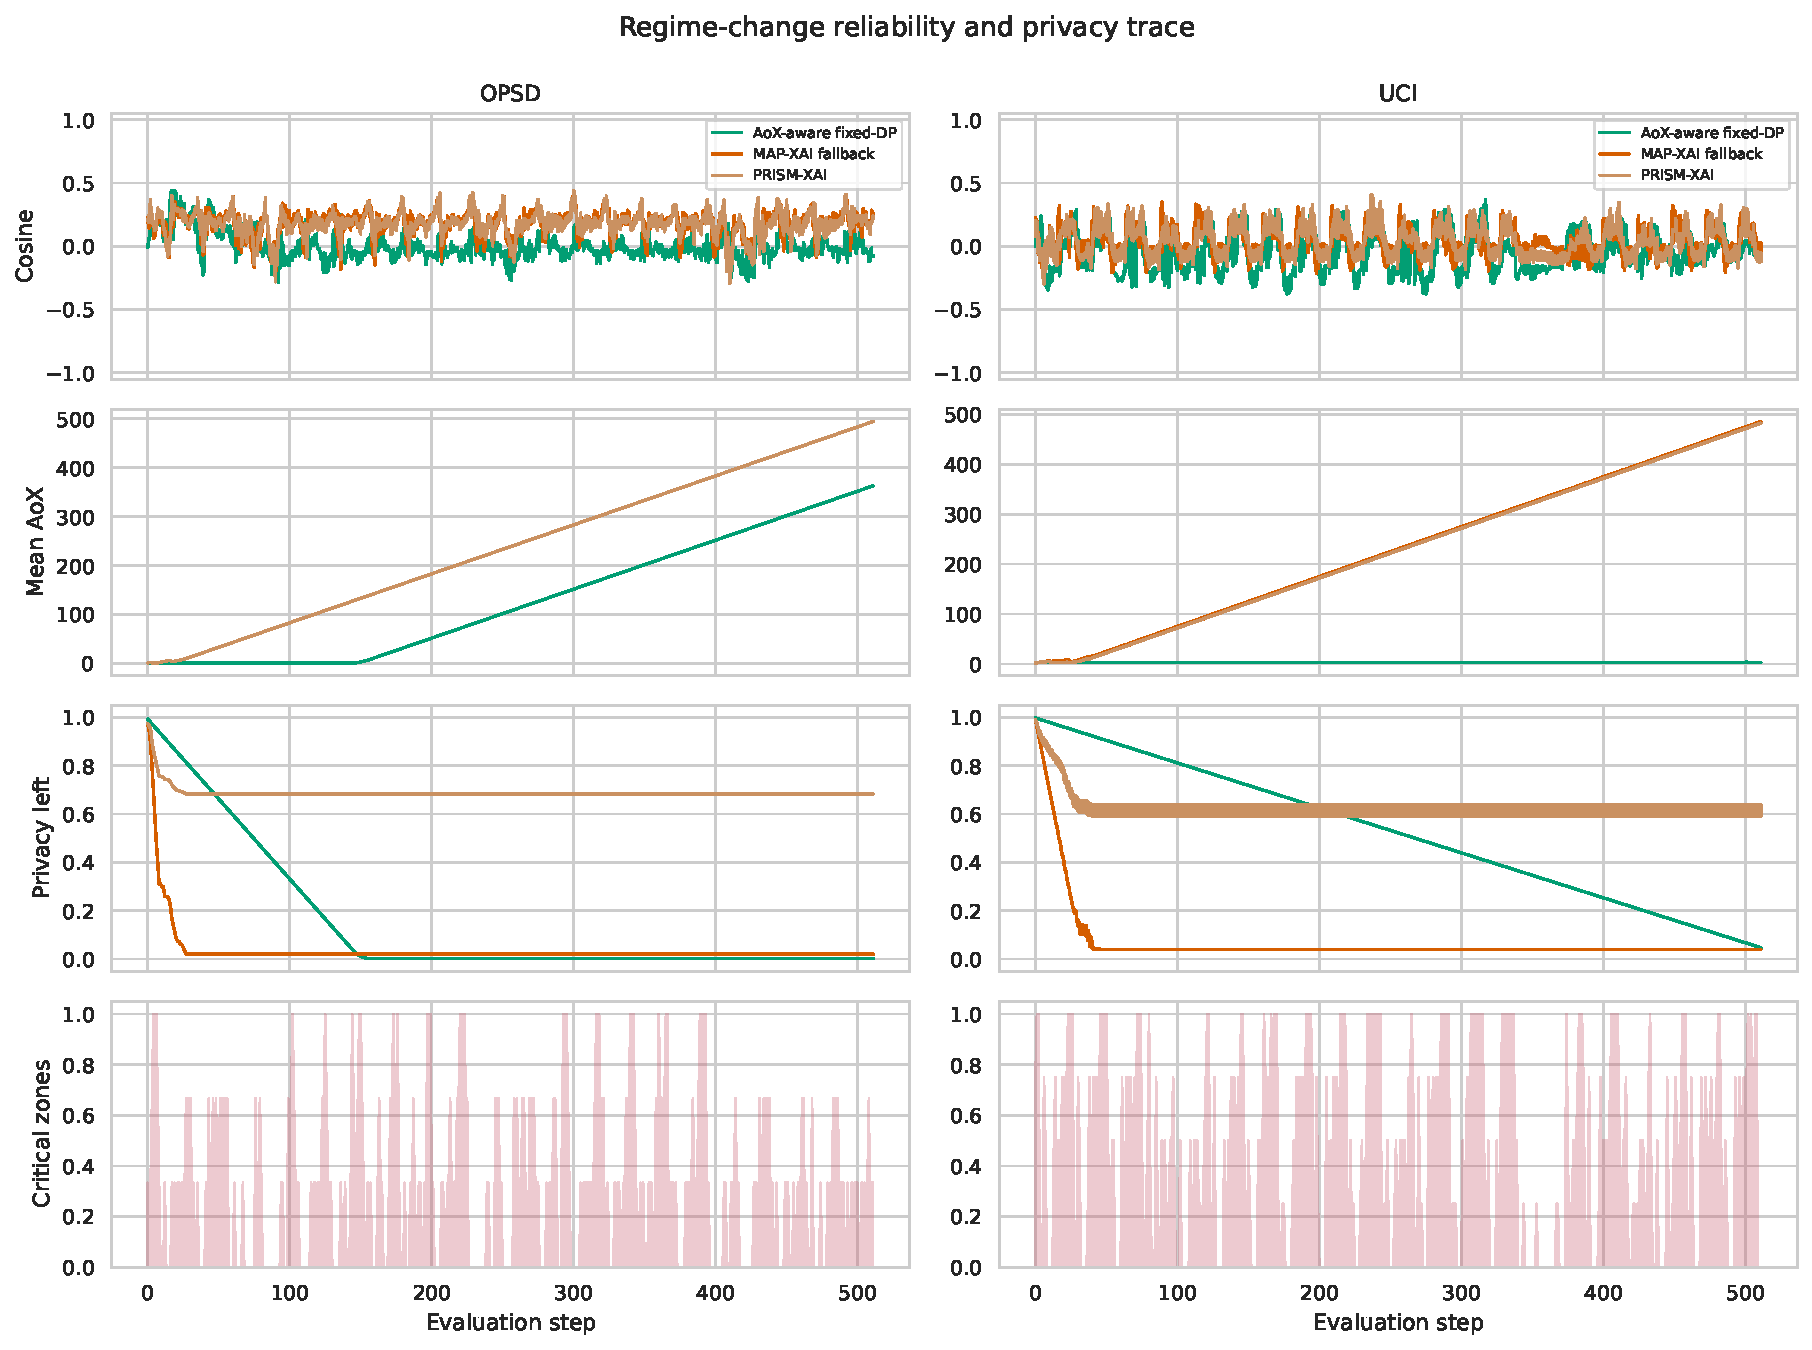
\includegraphics[width=.96\textwidth,height=.82\textheight,keepaspectratio]{../../SERVICE_TRADEOFF_RESULTS/runs/thr_1_cap_32/regime_trace.pdf}

\caption{Public-score threshold $\tau=1$, release cap $M=32$, Combined datasets: representative regime trace. This panel should be read with the setting-level quantitative interpretation and the complete tables immediately preceding the figure block.}

\end{figure*}

\clearpage

\begin{figure*}[p]

\centering

\includegraphics[width=.96\textwidth,height=.82\textheight,keepaspectratio]{../../SERVICE_TRADEOFF_RESULTS/runs/thr_1_cap_32/fairness_reliability.pdf}

\caption{Public-score threshold $\tau=1$, release cap $M=32$, Combined datasets: fairness--reliability plane. This panel should be read with the setting-level quantitative interpretation and the complete tables immediately preceding the figure block.}

\end{figure*}

\clearpage

\begin{figure*}[p]

\centering

\includegraphics[width=.96\textwidth,height=.82\textheight,keepaspectratio]{../../SERVICE_TRADEOFF_RESULTS/runs/thr_1_cap_32/privacy_fidelity.pdf}

\caption{Public-score threshold $\tau=1$, release cap $M=32$, Combined datasets: privacy--fidelity plane. This panel should be read with the setting-level quantitative interpretation and the complete tables immediately preceding the figure block.}

\end{figure*}

\clearpage

\begin{figure*}[p]

\centering

\includegraphics[width=.96\textwidth,height=.82\textheight,keepaspectratio]{../../SERVICE_TRADEOFF_RESULTS/runs/thr_1_cap_32/pareto_bits_fidelity.pdf}

\caption{Public-score threshold $\tau=1$, release cap $M=32$, Combined datasets: traffic--fidelity Pareto plane. This panel should be read with the setting-level quantitative interpretation and the complete tables immediately preceding the figure block.}

\end{figure*}

\clearpage

\begin{figure*}[p]

\centering

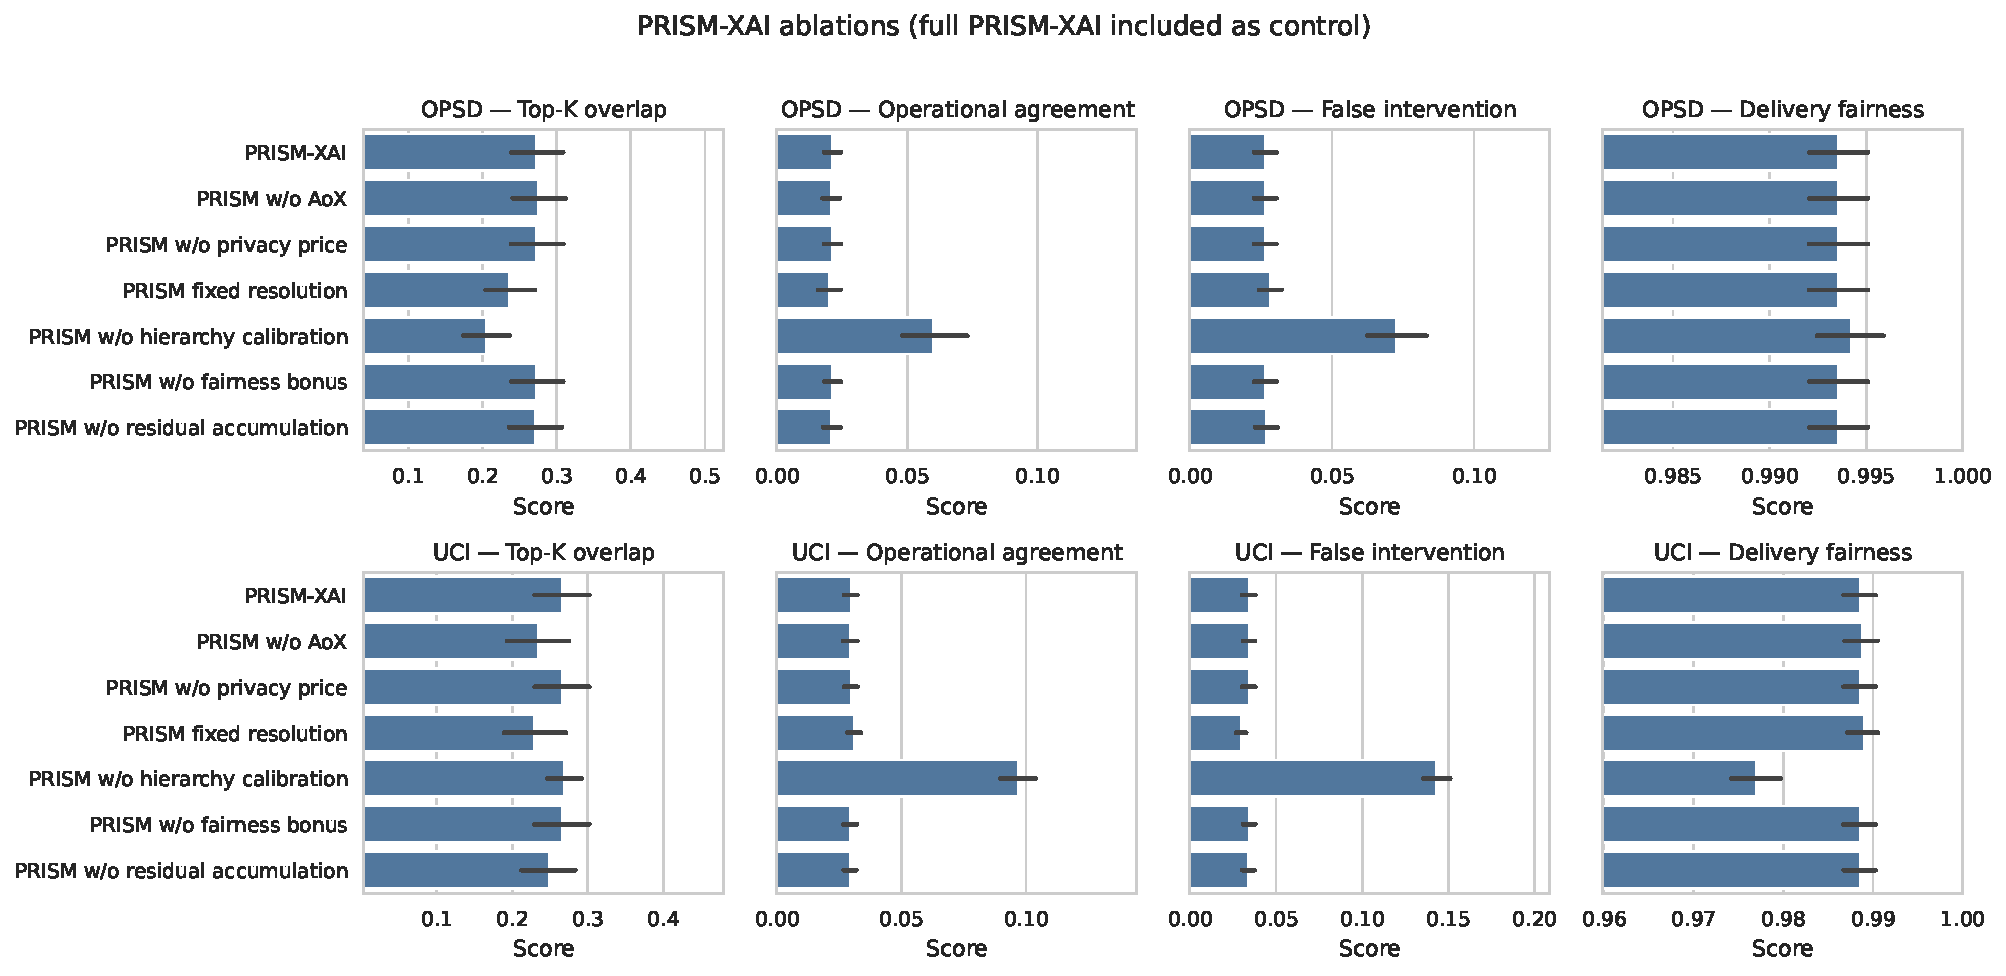
\includegraphics[width=.96\textwidth,height=.82\textheight,keepaspectratio]{../../SERVICE_TRADEOFF_RESULTS/runs/thr_1_cap_32/ablation_results.pdf}

\caption{Public-score threshold $\tau=1$, release cap $M=32$, Combined datasets: component ablation. This panel should be read with the setting-level quantitative interpretation and the complete tables immediately preceding the figure block.}

\end{figure*}

\clearpage

\paragraph{OPSD.} The three generated tables below report the full method means, all condition-level values, and paired differences. The five figures that follow provide the corresponding temporal, fairness, privacy, Pareto, and ablation views. Aggregate panels support the setting-level summary above; dataset panels reveal whether that summary is shared by OPSD and UCI rather than being driven by their different endpoint counts.

\begin{table*}[p]\centering\tiny

\caption{Public-score threshold $\tau=1$, release cap $M=32$, OPSD: complete generated method table.}

\label{tab:thr_1_cap_32:opsd:main}

\resizebox{\linewidth}{!}{% Values are means with 95% Student-t confidence intervals across seeds.
\begin{tabular}{lccccccccccccccc}
\toprule
Dataset & Model & $\epsilon_{\max}$ & Method & Top-$K$ & Cosine & Decision & Recall & Prec. & Abst. & P95 ms & kbit & Spent $\epsilon$ & False int. & bit/correct & Fairness \\
\midrule
OPSD & Tree & 8 & AoX-aware fixed-DP & 0.234 $\pm$ 0.048 & -0.033 $\pm$ 0.028 & 0.119 $\pm$ 0.028 & 0.119 $\pm$ 0.028 & 0.198 $\pm$ 0.054 & 0.721 $\pm$ 0.005 & 6.903 $\pm$ 1.126 & 1560.564 $\pm$ 0.000 & 7.990 $\pm$ 0.000 & 0.183 $\pm$ 0.020 & 35567.482 $\pm$ 10569.818 & 0.999 $\pm$ 0.000 \\
OPSD & Tree & 8 & AoX-aware fixed-DP & 0.238 $\pm$ 0.049 & -0.026 $\pm$ 0.055 & 0.121 $\pm$ 0.026 & 0.121 $\pm$ 0.026 & 0.205 $\pm$ 0.053 & 0.721 $\pm$ 0.005 & 6.903 $\pm$ 1.126 & 1560.564 $\pm$ 0.000 & 7.990 $\pm$ 0.000 & 0.179 $\pm$ 0.023 & 34123.214 $\pm$ 8376.542 & 0.999 $\pm$ 0.000 \\
OPSD & Tree & 8 & Channel-aware fixed-DP & 0.292 $\pm$ 0.037 & -0.041 $\pm$ 0.051 & 0.107 $\pm$ 0.026 & 0.107 $\pm$ 0.026 & 0.217 $\pm$ 0.068 & 0.779 $\pm$ 0.011 & 5.571 $\pm$ 1.784 & 1560.564 $\pm$ 0.000 & 7.990 $\pm$ 0.000 & 0.154 $\pm$ 0.029 & 40860.756 $\pm$ 14126.920 & 0.999 $\pm$ 0.000 \\
OPSD & Tree & 8 & Channel-aware fixed-DP & 0.292 $\pm$ 0.054 & -0.049 $\pm$ 0.064 & 0.111 $\pm$ 0.023 & 0.111 $\pm$ 0.023 & 0.228 $\pm$ 0.066 & 0.779 $\pm$ 0.011 & 5.571 $\pm$ 1.784 & 1560.564 $\pm$ 0.000 & 7.990 $\pm$ 0.000 & 0.149 $\pm$ 0.026 & 37980.855 $\pm$ 12338.094 & 0.999 $\pm$ 0.000 \\
OPSD & Tree & 8 & Joint, no compression & 0.288 $\pm$ 0.064 & -0.030 $\pm$ 0.079 & 0.016 $\pm$ 0.005 & 0.016 $\pm$ 0.005 & 0.193 $\pm$ 0.059 & 0.957 $\pm$ 0.003 & 4.560 $\pm$ 1.811 & 189.900 $\pm$ 0.554 & 7.990 $\pm$ 0.000 & 0.027 $\pm$ 0.005 & 32490.357 $\pm$ 10149.755 & 0.996 $\pm$ 0.002 \\
OPSD & Tree & 8 & Joint, no compression & 0.258 $\pm$ 0.055 & 0.011 $\pm$ 0.094 & 0.019 $\pm$ 0.004 & 0.019 $\pm$ 0.004 & 0.224 $\pm$ 0.044 & 0.957 $\pm$ 0.003 & 4.562 $\pm$ 1.809 & 189.750 $\pm$ 0.566 & 7.990 $\pm$ 0.000 & 0.025 $\pm$ 0.003 & 26079.167 $\pm$ 6335.386 & 0.996 $\pm$ 0.002 \\
OPSD & Tree & 8 & Periodic fixed-DP & 0.241 $\pm$ 0.049 & -0.019 $\pm$ 0.061 & 0.125 $\pm$ 0.020 & 0.125 $\pm$ 0.020 & 0.209 $\pm$ 0.044 & 0.722 $\pm$ 0.006 & 6.303 $\pm$ 1.438 & 1560.564 $\pm$ 0.000 & 7.990 $\pm$ 0.000 & 0.181 $\pm$ 0.021 & 31183.082 $\pm$ 4356.378 & 0.999 $\pm$ 0.000 \\
OPSD & Tree & 8 & Periodic fixed-DP & 0.242 $\pm$ 0.048 & -0.026 $\pm$ 0.082 & 0.135 $\pm$ 0.016 & 0.135 $\pm$ 0.016 & 0.231 $\pm$ 0.037 & 0.722 $\pm$ 0.006 & 6.303 $\pm$ 1.438 & 1560.564 $\pm$ 0.000 & 7.990 $\pm$ 0.000 & 0.169 $\pm$ 0.017 & 28520.235 $\pm$ 3511.595 & 0.999 $\pm$ 0.000 \\
OPSD & Tree & 8 & PRISM-XAI & 0.261 $\pm$ 0.053 & -0.019 $\pm$ 0.080 & 0.021 $\pm$ 0.005 & 0.021 $\pm$ 0.005 & 0.246 $\pm$ 0.094 & 0.947 $\pm$ 0.003 & 4.452 $\pm$ 1.878 & 97.640 $\pm$ 0.539 & 5.377 $\pm$ 0.416 & 0.027 $\pm$ 0.007 & 13250.048 $\pm$ 5126.243 & 0.994 $\pm$ 0.003 \\
OPSD & Tree & 8 & PRISM-XAI & 0.284 $\pm$ 0.064 & -0.006 $\pm$ 0.076 & 0.022 $\pm$ 0.005 & 0.022 $\pm$ 0.005 & 0.253 $\pm$ 0.080 & 0.947 $\pm$ 0.003 & 4.452 $\pm$ 1.878 & 97.251 $\pm$ 0.416 & 5.108 $\pm$ 0.367 & 0.026 $\pm$ 0.006 & 12180.416 $\pm$ 3594.328 & 0.994 $\pm$ 0.003 \\
OPSD & Tree & 8 & MAP-XAI fallback & 0.249 $\pm$ 0.062 & -0.025 $\pm$ 0.053 & 0.019 $\pm$ 0.007 & 0.019 $\pm$ 0.007 & 0.212 $\pm$ 0.098 & 0.947 $\pm$ 0.003 & 4.568 $\pm$ 1.808 & 117.817 $\pm$ 0.049 & 7.924 $\pm$ 0.000 & 0.030 $\pm$ 0.007 & 25854.893 $\pm$ 23642.714 & 0.994 $\pm$ 0.003 \\
OPSD & Tree & 8 & MAP-XAI fallback & 0.233 $\pm$ 0.051 & 0.005 $\pm$ 0.068 & 0.022 $\pm$ 0.007 & 0.022 $\pm$ 0.007 & 0.257 $\pm$ 0.098 & 0.947 $\pm$ 0.003 & 4.568 $\pm$ 1.808 & 117.675 $\pm$ 0.049 & 7.924 $\pm$ 0.000 & 0.026 $\pm$ 0.007 & 18081.688 $\pm$ 11158.136 & 0.994 $\pm$ 0.003 \\
\bottomrule
\end{tabular}
}

\end{table*}\clearpage

\begin{table*}[p]\centering\tiny

\caption{Public-score threshold $\tau=1$, release cap $M=32$, OPSD: complete condition-level generated table.}

\label{tab:thr_1_cap_32:opsd:conditions}

\resizebox{\textwidth}{!}{\begin{tabular}{llllccccccccccc}
\toprule
Dataset & Model & $\epsilon_{\max}$ & Method & kbit & Top-$K$ & Random Top-$K$ & Cosine & Decision & Recall & Precision & Coverage & Abstain & False int. & Spent $\epsilon$ \\
\midrule
OPSD & Tree & 8 & Joint, no compression & 189.900 $\pm$ 0.554 & 0.288 $\pm$ 0.064 & 0.250 $\pm$ 0.000 & -0.030 $\pm$ 0.079 & 0.016 $\pm$ 0.005 & 0.016 $\pm$ 0.005 & 0.193 $\pm$ 0.059 & 0.043 $\pm$ 0.003 & 0.957 $\pm$ 0.003 & 0.027 $\pm$ 0.005 & 7.990 $\pm$ 0.000 \\
OPSD & Tree & 8 & Joint, no compression & 189.750 $\pm$ 0.566 & 0.258 $\pm$ 0.055 & 0.250 $\pm$ 0.000 & 0.011 $\pm$ 0.094 & 0.019 $\pm$ 0.004 & 0.019 $\pm$ 0.004 & 0.224 $\pm$ 0.044 & 0.043 $\pm$ 0.003 & 0.957 $\pm$ 0.003 & 0.025 $\pm$ 0.003 & 7.990 $\pm$ 0.000 \\
OPSD & Tree & 8 & Periodic fixed-DP & 1560.564 $\pm$ 0.000 & 0.241 $\pm$ 0.049 & 0.250 $\pm$ 0.000 & -0.019 $\pm$ 0.061 & 0.125 $\pm$ 0.020 & 0.125 $\pm$ 0.020 & 0.209 $\pm$ 0.044 & 0.278 $\pm$ 0.006 & 0.722 $\pm$ 0.006 & 0.181 $\pm$ 0.021 & 7.990 $\pm$ 0.000 \\
OPSD & Tree & 8 & Periodic fixed-DP & 1560.564 $\pm$ 0.000 & 0.242 $\pm$ 0.048 & 0.250 $\pm$ 0.000 & -0.026 $\pm$ 0.082 & 0.135 $\pm$ 0.016 & 0.135 $\pm$ 0.016 & 0.231 $\pm$ 0.037 & 0.278 $\pm$ 0.006 & 0.722 $\pm$ 0.006 & 0.169 $\pm$ 0.017 & 7.990 $\pm$ 0.000 \\
OPSD & Tree & 8 & PRISM-XAI & 97.640 $\pm$ 0.539 & 0.261 $\pm$ 0.053 & 0.250 $\pm$ 0.000 & -0.019 $\pm$ 0.080 & 0.021 $\pm$ 0.005 & 0.021 $\pm$ 0.005 & 0.246 $\pm$ 0.094 & 0.053 $\pm$ 0.003 & 0.947 $\pm$ 0.003 & 0.027 $\pm$ 0.007 & 5.377 $\pm$ 0.416 \\
OPSD & Tree & 8 & PRISM-XAI & 97.251 $\pm$ 0.416 & 0.284 $\pm$ 0.064 & 0.250 $\pm$ 0.000 & -0.006 $\pm$ 0.076 & 0.022 $\pm$ 0.005 & 0.022 $\pm$ 0.005 & 0.253 $\pm$ 0.080 & 0.053 $\pm$ 0.003 & 0.947 $\pm$ 0.003 & 0.026 $\pm$ 0.006 & 5.108 $\pm$ 0.367 \\
OPSD & Tree & 16 & Joint, no compression & 459.900 $\pm$ 0.750 & 0.232 $\pm$ 0.065 & 0.250 $\pm$ 0.000 & 0.059 $\pm$ 0.048 & 0.038 $\pm$ 0.009 & 0.038 $\pm$ 0.009 & 0.222 $\pm$ 0.049 & 0.088 $\pm$ 0.004 & 0.912 $\pm$ 0.004 & 0.049 $\pm$ 0.005 & 15.997 $\pm$ 0.000 \\
OPSD & Tree & 16 & Joint, no compression & 460.050 $\pm$ 0.724 & 0.241 $\pm$ 0.055 & 0.250 $\pm$ 0.000 & 0.061 $\pm$ 0.052 & 0.039 $\pm$ 0.008 & 0.039 $\pm$ 0.008 & 0.241 $\pm$ 0.042 & 0.088 $\pm$ 0.004 & 0.912 $\pm$ 0.004 & 0.045 $\pm$ 0.004 & 15.997 $\pm$ 0.000 \\
OPSD & Tree & 16 & Periodic fixed-DP & 5112.594 $\pm$ 0.000 & 0.249 $\pm$ 0.022 & 0.250 $\pm$ 0.000 & -0.009 $\pm$ 0.045 & 0.450 $\pm$ 0.062 & 0.450 $\pm$ 0.062 & 0.237 $\pm$ 0.042 & 0.985 $\pm$ 0.002 & 0.015 $\pm$ 0.002 & 0.551 $\pm$ 0.057 & 15.997 $\pm$ 0.000 \\
OPSD & Tree & 16 & Periodic fixed-DP & 5112.594 $\pm$ 0.000 & 0.243 $\pm$ 0.019 & 0.250 $\pm$ 0.000 & -0.012 $\pm$ 0.050 & 0.463 $\pm$ 0.047 & 0.463 $\pm$ 0.047 & 0.240 $\pm$ 0.028 & 0.985 $\pm$ 0.002 & 0.015 $\pm$ 0.002 & 0.547 $\pm$ 0.036 & 15.997 $\pm$ 0.000 \\
OPSD & Tree & 16 & PRISM-XAI & 296.336 $\pm$ 0.924 & 0.239 $\pm$ 0.051 & 0.250 $\pm$ 0.000 & 0.018 $\pm$ 0.080 & 0.059 $\pm$ 0.016 & 0.059 $\pm$ 0.016 & 0.259 $\pm$ 0.080 & 0.134 $\pm$ 0.004 & 0.866 $\pm$ 0.004 & 0.066 $\pm$ 0.012 & 14.393 $\pm$ 0.046 \\
OPSD & Tree & 16 & PRISM-XAI & 295.240 $\pm$ 0.855 & 0.226 $\pm$ 0.027 & 0.250 $\pm$ 0.000 & 0.001 $\pm$ 0.087 & 0.061 $\pm$ 0.015 & 0.061 $\pm$ 0.015 & 0.274 $\pm$ 0.080 & 0.134 $\pm$ 0.004 & 0.866 $\pm$ 0.004 & 0.065 $\pm$ 0.014 & 14.360 $\pm$ 0.035 \\
OPSD & Tree & 32 & Joint, no compression & 1140.900 $\pm$ 7.953 & 0.235 $\pm$ 0.064 & 0.250 $\pm$ 0.000 & -0.031 $\pm$ 0.089 & 0.074 $\pm$ 0.015 & 0.074 $\pm$ 0.015 & 0.205 $\pm$ 0.039 & 0.157 $\pm$ 0.006 & 0.843 $\pm$ 0.006 & 0.107 $\pm$ 0.009 & 31.999 $\pm$ 0.000 \\
OPSD & Tree & 32 & Joint, no compression & 1140.900 $\pm$ 7.953 & 0.282 $\pm$ 0.054 & 0.250 $\pm$ 0.000 & -0.044 $\pm$ 0.076 & 0.080 $\pm$ 0.011 & 0.080 $\pm$ 0.011 & 0.227 $\pm$ 0.052 & 0.158 $\pm$ 0.006 & 0.842 $\pm$ 0.006 & 0.105 $\pm$ 0.015 & 31.999 $\pm$ 0.000 \\
OPSD & Tree & 32 & Periodic fixed-DP & 5299.836 $\pm$ 0.625 & 0.249 $\pm$ 0.022 & 0.250 $\pm$ 0.000 & -0.009 $\pm$ 0.044 & 0.458 $\pm$ 0.066 & 0.458 $\pm$ 0.066 & 0.237 $\pm$ 0.045 & 1.000 $\pm$ 0.000 & 0.000 $\pm$ 0.000 & 0.562 $\pm$ 0.062 & 16.371 $\pm$ 0.000 \\
OPSD & Tree & 32 & Periodic fixed-DP & 5299.836 $\pm$ 0.625 & 0.244 $\pm$ 0.019 & 0.250 $\pm$ 0.000 & -0.012 $\pm$ 0.050 & 0.471 $\pm$ 0.049 & 0.471 $\pm$ 0.049 & 0.240 $\pm$ 0.029 & 1.000 $\pm$ 0.000 & 0.000 $\pm$ 0.000 & 0.559 $\pm$ 0.039 & 16.371 $\pm$ 0.000 \\
OPSD & Tree & 32 & PRISM-XAI & 350.911 $\pm$ 0.837 & 0.222 $\pm$ 0.050 & 0.250 $\pm$ 0.000 & 0.012 $\pm$ 0.068 & 0.062 $\pm$ 0.017 & 0.062 $\pm$ 0.017 & 0.228 $\pm$ 0.070 & 0.140 $\pm$ 0.005 & 0.860 $\pm$ 0.005 & 0.082 $\pm$ 0.015 & 31.175 $\pm$ 0.000 \\
OPSD & Tree & 32 & PRISM-XAI & 349.693 $\pm$ 0.728 & 0.243 $\pm$ 0.064 & 0.250 $\pm$ 0.000 & 0.019 $\pm$ 0.085 & 0.060 $\pm$ 0.016 & 0.060 $\pm$ 0.016 & 0.233 $\pm$ 0.084 & 0.140 $\pm$ 0.005 & 0.860 $\pm$ 0.005 & 0.081 $\pm$ 0.019 & 31.175 $\pm$ 0.000 \\
\bottomrule
\end{tabular}
}

\end{table*}\clearpage

\begin{table*}[p]\centering\tiny

\caption{Public-score threshold $\tau=1$, release cap $M=32$, OPSD: complete generated paired comparisons.}

\label{tab:thr_1_cap_32:opsd:paired}

\resizebox{\textwidth}{!}{\begin{tabular}{llcccc}
\toprule
Dataset & Baseline & Delta kbit & Delta Top-$K$ & Delta recall & Delta fairness \\
\midrule
OPSD & AoX-aware fixed-DP & -1462.924 $\pm$ 0.539 & 0.027 $\pm$ 0.083 & -0.099 $\pm$ 0.029 & -0.006 $\pm$ 0.003 \\
OPSD & AoX-aware fixed-DP & -4803.577 $\pm$ 5.551 & -0.015 $\pm$ 0.045 & -0.343 $\pm$ 0.075 & -0.003 $\pm$ 0.002 \\
OPSD & AoX-aware fixed-DP & -4949.313 $\pm$ 0.837 & -0.030 $\pm$ 0.066 & -0.350 $\pm$ 0.078 & -0.002 $\pm$ 0.001 \\
OPSD & AoX-aware fixed-DP & -1463.313 $\pm$ 0.416 & 0.046 $\pm$ 0.054 & -0.099 $\pm$ 0.026 & -0.006 $\pm$ 0.003 \\
OPSD & AoX-aware fixed-DP & -4804.672 $\pm$ 5.519 & -0.026 $\pm$ 0.034 & -0.353 $\pm$ 0.061 & -0.003 $\pm$ 0.002 \\
OPSD & AoX-aware fixed-DP & -4950.531 $\pm$ 0.728 & -0.009 $\pm$ 0.071 & -0.365 $\pm$ 0.060 & -0.002 $\pm$ 0.001 \\
OPSD & Channel-aware fixed-DP & -1462.924 $\pm$ 0.539 & -0.032 $\pm$ 0.060 & -0.086 $\pm$ 0.026 & -0.006 $\pm$ 0.003 \\
OPSD & Channel-aware fixed-DP & -4390.274 $\pm$ 13.308 & -0.023 $\pm$ 0.044 & -0.343 $\pm$ 0.094 & 0.060 $\pm$ 0.005 \\
OPSD & Channel-aware fixed-DP & -4949.313 $\pm$ 0.837 & -0.035 $\pm$ 0.059 & -0.372 $\pm$ 0.099 & 0.091 $\pm$ 0.005 \\
OPSD & Channel-aware fixed-DP & -1463.313 $\pm$ 0.416 & -0.008 $\pm$ 0.077 & -0.090 $\pm$ 0.024 & -0.006 $\pm$ 0.003 \\
OPSD & Channel-aware fixed-DP & -4391.369 $\pm$ 13.318 & -0.032 $\pm$ 0.032 & -0.358 $\pm$ 0.092 & 0.060 $\pm$ 0.005 \\
OPSD & Channel-aware fixed-DP & -4950.531 $\pm$ 0.728 & -0.014 $\pm$ 0.068 & -0.396 $\pm$ 0.091 & 0.091 $\pm$ 0.005 \\
OPSD & Joint, no compression & -92.260 $\pm$ 0.532 & -0.027 $\pm$ 0.058 & 0.004 $\pm$ 0.006 & -0.002 $\pm$ 0.002 \\
OPSD & Joint, no compression & -163.565 $\pm$ 1.527 & 0.007 $\pm$ 0.064 & 0.021 $\pm$ 0.012 & 0.000 $\pm$ 0.001 \\
OPSD & Joint, no compression & -789.989 $\pm$ 8.405 & -0.013 $\pm$ 0.095 & -0.012 $\pm$ 0.017 & -0.001 $\pm$ 0.001 \\
OPSD & Joint, no compression & -92.499 $\pm$ 0.556 & 0.026 $\pm$ 0.104 & 0.003 $\pm$ 0.003 & -0.002 $\pm$ 0.002 \\
OPSD & Joint, no compression & -164.810 $\pm$ 1.425 & -0.014 $\pm$ 0.044 & 0.022 $\pm$ 0.014 & 0.000 $\pm$ 0.001 \\
OPSD & Joint, no compression & -791.207 $\pm$ 8.350 & -0.039 $\pm$ 0.094 & -0.020 $\pm$ 0.015 & -0.001 $\pm$ 0.001 \\
OPSD & Periodic fixed-DP & -1462.924 $\pm$ 0.539 & 0.020 $\pm$ 0.076 & -0.104 $\pm$ 0.021 & -0.006 $\pm$ 0.003 \\
OPSD & Periodic fixed-DP & -4816.259 $\pm$ 0.924 & -0.011 $\pm$ 0.051 & -0.392 $\pm$ 0.064 & -0.003 $\pm$ 0.002 \\
OPSD & Periodic fixed-DP & -4948.925 $\pm$ 0.865 & -0.027 $\pm$ 0.061 & -0.396 $\pm$ 0.066 & -0.002 $\pm$ 0.001 \\
OPSD & Periodic fixed-DP & -1463.313 $\pm$ 0.416 & 0.043 $\pm$ 0.057 & -0.113 $\pm$ 0.016 & -0.006 $\pm$ 0.003 \\
OPSD & Periodic fixed-DP & -4817.354 $\pm$ 0.855 & -0.017 $\pm$ 0.029 & -0.402 $\pm$ 0.055 & -0.003 $\pm$ 0.002 \\
OPSD & Periodic fixed-DP & -4950.143 $\pm$ 0.776 & -0.000 $\pm$ 0.065 & -0.411 $\pm$ 0.052 & -0.002 $\pm$ 0.001 \\
OPSD & MAP-XAI fallback & -20.177 $\pm$ 0.549 & 0.012 $\pm$ 0.081 & 0.001 $\pm$ 0.005 & 0.000 $\pm$ 0.000 \\
OPSD & MAP-XAI fallback & -65.981 $\pm$ 0.926 & 0.031 $\pm$ 0.045 & 0.002 $\pm$ 0.004 & 0.000 $\pm$ 0.000 \\
OPSD & MAP-XAI fallback & -78.906 $\pm$ 0.839 & 0.007 $\pm$ 0.030 & 0.002 $\pm$ 0.009 & 0.000 $\pm$ 0.000 \\
OPSD & MAP-XAI fallback & -20.424 $\pm$ 0.409 & 0.051 $\pm$ 0.064 & -0.000 $\pm$ 0.006 & 0.000 $\pm$ 0.000 \\
OPSD & MAP-XAI fallback & -66.935 $\pm$ 0.867 & 0.017 $\pm$ 0.028 & 0.005 $\pm$ 0.005 & 0.000 $\pm$ 0.000 \\
OPSD & MAP-XAI fallback & -79.982 $\pm$ 0.736 & 0.019 $\pm$ 0.017 & 0.001 $\pm$ 0.009 & 0.000 $\pm$ 0.000 \\
\bottomrule
\end{tabular}
}

\end{table*}\clearpage

\begin{figure*}[p]

\centering

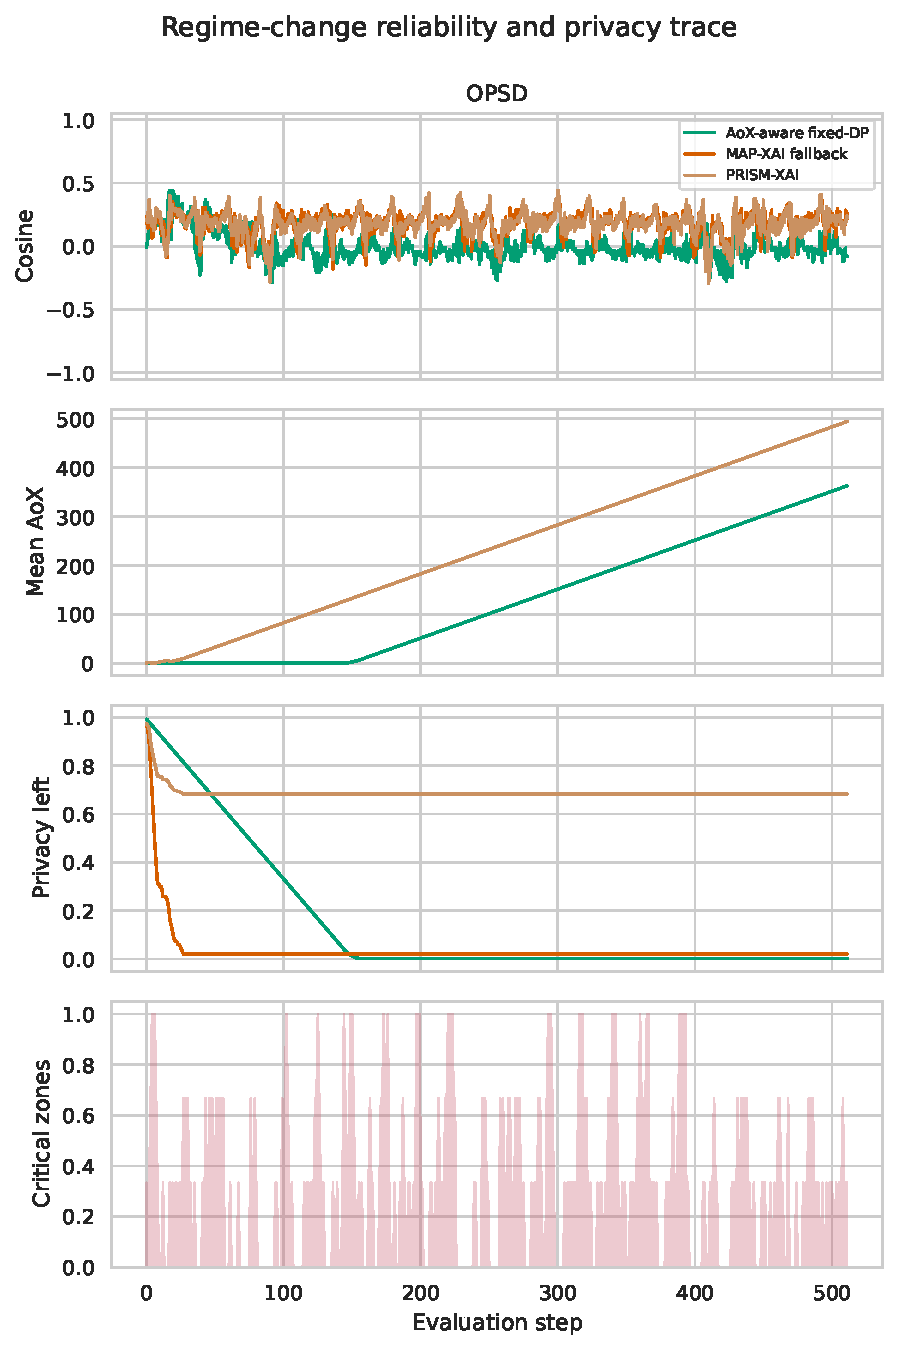
\includegraphics[width=.96\textwidth,height=.82\textheight,keepaspectratio]{../../SERVICE_TRADEOFF_RESULTS/runs/thr_1_cap_32/opsd/regime_trace.pdf}

\caption{Public-score threshold $\tau=1$, release cap $M=32$, OPSD: representative regime trace. This panel should be read with the setting-level quantitative interpretation and the complete tables immediately preceding the figure block.}

\end{figure*}

\clearpage

\begin{figure*}[p]

\centering

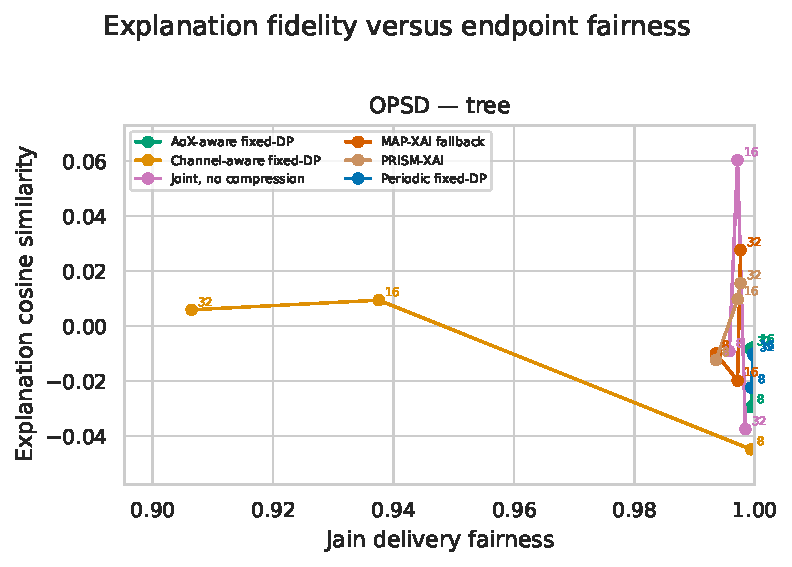
\includegraphics[width=.96\textwidth,height=.82\textheight,keepaspectratio]{../../SERVICE_TRADEOFF_RESULTS/runs/thr_1_cap_32/opsd/fairness_reliability.pdf}

\caption{Public-score threshold $\tau=1$, release cap $M=32$, OPSD: fairness--reliability plane. This panel should be read with the setting-level quantitative interpretation and the complete tables immediately preceding the figure block.}

\end{figure*}

\clearpage

\begin{figure*}[p]

\centering

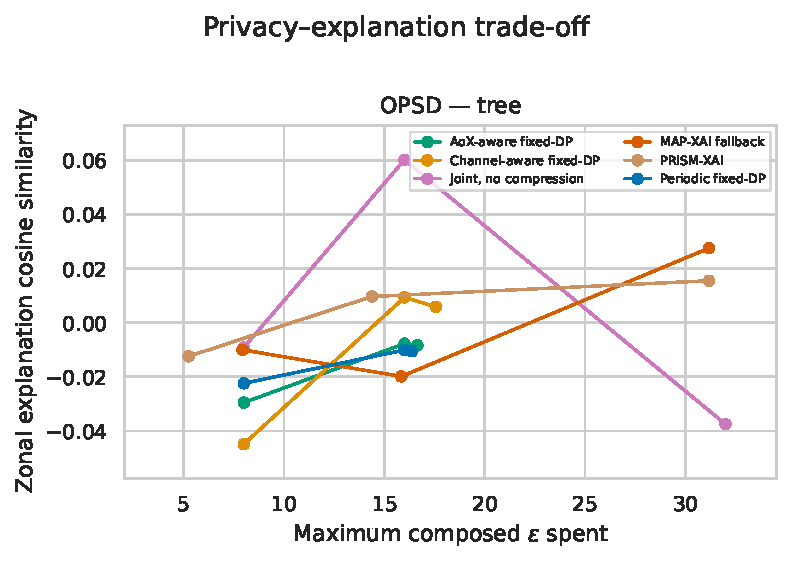
\includegraphics[width=.96\textwidth,height=.82\textheight,keepaspectratio]{../../SERVICE_TRADEOFF_RESULTS/runs/thr_1_cap_32/opsd/privacy_fidelity.pdf}

\caption{Public-score threshold $\tau=1$, release cap $M=32$, OPSD: privacy--fidelity plane. This panel should be read with the setting-level quantitative interpretation and the complete tables immediately preceding the figure block.}

\end{figure*}

\clearpage

\begin{figure*}[p]

\centering

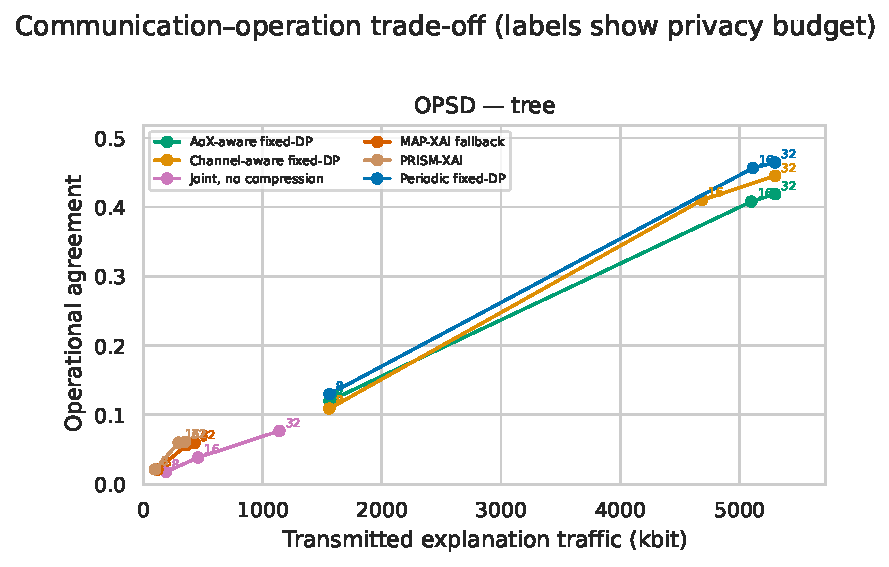
\includegraphics[width=.96\textwidth,height=.82\textheight,keepaspectratio]{../../SERVICE_TRADEOFF_RESULTS/runs/thr_1_cap_32/opsd/pareto_bits_fidelity.pdf}

\caption{Public-score threshold $\tau=1$, release cap $M=32$, OPSD: traffic--fidelity Pareto plane. This panel should be read with the setting-level quantitative interpretation and the complete tables immediately preceding the figure block.}

\end{figure*}

\clearpage

\begin{figure*}[p]

\centering

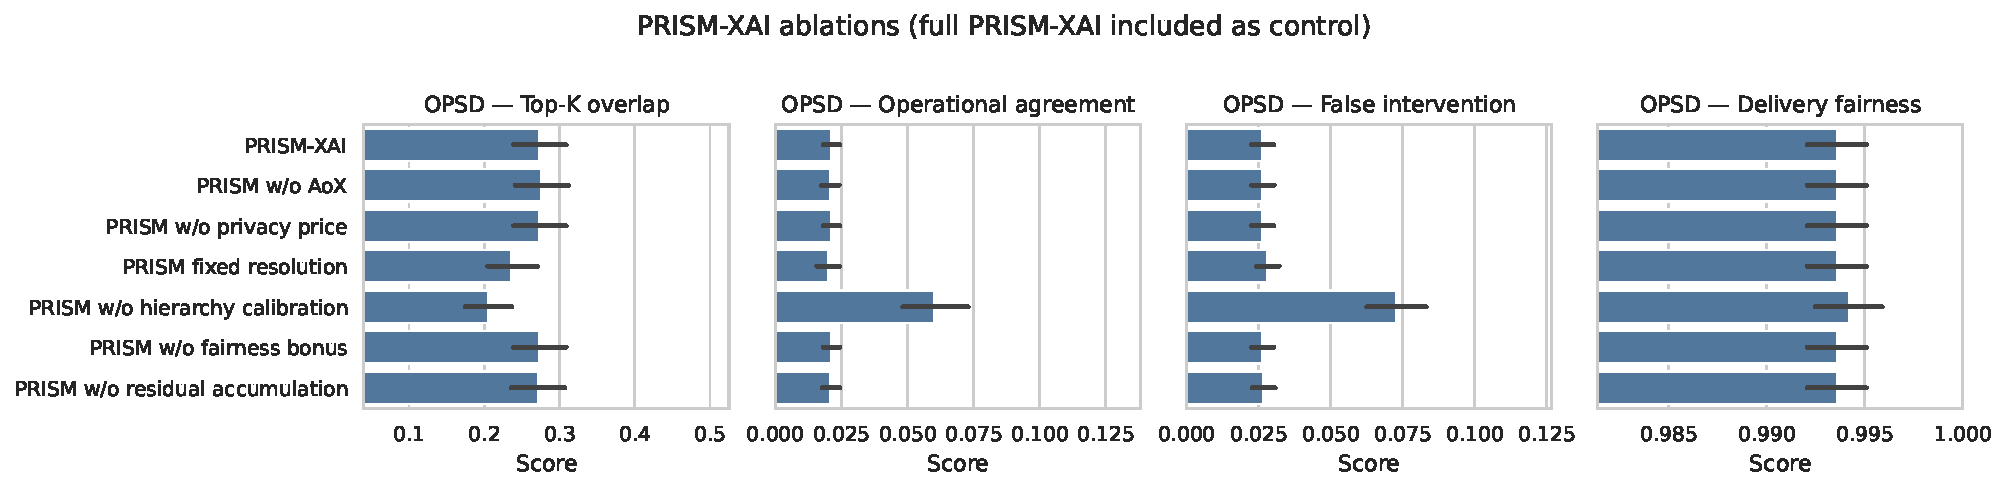
\includegraphics[width=.96\textwidth,height=.82\textheight,keepaspectratio]{../../SERVICE_TRADEOFF_RESULTS/runs/thr_1_cap_32/opsd/ablation_results.pdf}

\caption{Public-score threshold $\tau=1$, release cap $M=32$, OPSD: component ablation. This panel should be read with the setting-level quantitative interpretation and the complete tables immediately preceding the figure block.}

\end{figure*}

\clearpage

\paragraph{UCI.} The three generated tables below report the full method means, all condition-level values, and paired differences. The five figures that follow provide the corresponding temporal, fairness, privacy, Pareto, and ablation views. Aggregate panels support the setting-level summary above; dataset panels reveal whether that summary is shared by OPSD and UCI rather than being driven by their different endpoint counts.

\begin{table*}[p]\centering\tiny

\caption{Public-score threshold $\tau=1$, release cap $M=32$, UCI: complete generated method table.}

\label{tab:thr_1_cap_32:uci:main}

\resizebox{\linewidth}{!}{% Values are means with 95% Student-t confidence intervals across seeds.
\begin{tabular}{lccccccccccccccc}
\toprule
Dataset & Model & $\epsilon_{\max}$ & Method & Top-$K$ & Cosine & Decision & Recall & Prec. & Abst. & P95 ms & kbit & Spent $\epsilon$ & False int. & bit/correct & Fairness \\
\midrule
UCI & Tree & 8 & AoX-aware fixed-DP & 0.263 $\pm$ 0.041 & -0.007 $\pm$ 0.009 & 0.457 $\pm$ 0.031 & 0.457 $\pm$ 0.031 & 0.362 $\pm$ 0.024 & 0.003 $\pm$ 0.001 & 7.500 $\pm$ 0.000 & 5300.224 $\pm$ 0.000 & 7.990 $\pm$ 0.000 & 0.557 $\pm$ 0.025 & 14002.896 $\pm$ 1040.243 & 0.999 $\pm$ 0.000 \\
UCI & Tree & 8 & AoX-aware fixed-DP & 0.260 $\pm$ 0.022 & 0.010 $\pm$ 0.055 & 0.455 $\pm$ 0.047 & 0.455 $\pm$ 0.047 & 0.361 $\pm$ 0.038 & 0.003 $\pm$ 0.001 & 7.500 $\pm$ 0.000 & 5300.224 $\pm$ 0.000 & 7.990 $\pm$ 0.000 & 0.557 $\pm$ 0.048 & 14198.303 $\pm$ 1508.274 & 0.999 $\pm$ 0.000 \\
UCI & Tree & 8 & Channel-aware fixed-DP & 0.248 $\pm$ 0.031 & 0.004 $\pm$ 0.012 & 0.001 $\pm$ 0.001 & 0.001 $\pm$ 0.001 & 0.150 $\pm$ 0.151 & 0.999 $\pm$ 0.001 & 4.609 $\pm$ 1.781 & 5295.177 $\pm$ 3.740 & 7.990 $\pm$ 0.000 & 0.001 $\pm$ 0.001 & 4632196.500 $\pm$ 2102650.252 & 0.991 $\pm$ 0.001 \\
UCI & Tree & 8 & Channel-aware fixed-DP & 0.239 $\pm$ 0.030 & -0.020 $\pm$ 0.055 & 0.000 $\pm$ 0.000 & 0.000 $\pm$ 0.000 & 0.117 $\pm$ 0.225 & 0.999 $\pm$ 0.001 & 4.609 $\pm$ 1.781 & 5295.177 $\pm$ 3.740 & 7.990 $\pm$ 0.000 & 0.001 $\pm$ 0.001 & 5296989.000 $\pm$ 41104.572 & 0.991 $\pm$ 0.001 \\
UCI & Tree & 8 & Joint, no compression & 0.286 $\pm$ 0.045 & 0.004 $\pm$ 0.020 & 0.052 $\pm$ 0.005 & 0.052 $\pm$ 0.005 & 0.406 $\pm$ 0.037 & 0.875 $\pm$ 0.003 & 5.123 $\pm$ 1.792 & 672.300 $\pm$ 0.452 & 7.990 $\pm$ 0.000 & 0.053 $\pm$ 0.004 & 15676.175 $\pm$ 1475.621 & 0.994 $\pm$ 0.003 \\
UCI & Tree & 8 & Joint, no compression & 0.229 $\pm$ 0.052 & -0.032 $\pm$ 0.050 & 0.057 $\pm$ 0.007 & 0.057 $\pm$ 0.007 & 0.428 $\pm$ 0.041 & 0.875 $\pm$ 0.003 & 5.131 $\pm$ 1.787 & 672.300 $\pm$ 0.452 & 7.990 $\pm$ 0.000 & 0.052 $\pm$ 0.004 & 14702.786 $\pm$ 2334.488 & 0.994 $\pm$ 0.003 \\
UCI & Tree & 8 & Periodic fixed-DP & 0.259 $\pm$ 0.060 & -0.005 $\pm$ 0.008 & 0.006 $\pm$ 0.001 & 0.006 $\pm$ 0.001 & 0.244 $\pm$ 0.049 & 0.989 $\pm$ 0.001 & 4.596 $\pm$ 1.788 & 5299.318 $\pm$ 1.451 & 7.786 $\pm$ 0.000 & 0.013 $\pm$ 0.002 & 1215103.896 $\pm$ 390671.319 & 0.999 $\pm$ 0.000 \\
UCI & Tree & 8 & Periodic fixed-DP & 0.260 $\pm$ 0.044 & 0.022 $\pm$ 0.070 & 0.005 $\pm$ 0.001 & 0.005 $\pm$ 0.001 & 0.195 $\pm$ 0.050 & 0.989 $\pm$ 0.001 & 4.596 $\pm$ 1.788 & 5299.318 $\pm$ 1.451 & 7.786 $\pm$ 0.000 & 0.015 $\pm$ 0.002 & 1555837.203 $\pm$ 955472.503 & 0.999 $\pm$ 0.000 \\
UCI & Tree & 8 & PRISM-XAI & 0.270 $\pm$ 0.078 & -0.004 $\pm$ 0.021 & 0.029 $\pm$ 0.006 & 0.029 $\pm$ 0.006 & 0.346 $\pm$ 0.060 & 0.928 $\pm$ 0.003 & 5.789 $\pm$ 1.601 & 333.552 $\pm$ 0.722 & 6.549 $\pm$ 0.228 & 0.037 $\pm$ 0.005 & 15343.847 $\pm$ 4327.572 & 0.989 $\pm$ 0.003 \\
UCI & Tree & 8 & PRISM-XAI & 0.262 $\pm$ 0.032 & -0.011 $\pm$ 0.061 & 0.031 $\pm$ 0.004 & 0.031 $\pm$ 0.004 & 0.416 $\pm$ 0.078 & 0.931 $\pm$ 0.004 & 4.104 $\pm$ 1.678 & 331.348 $\pm$ 1.358 & 6.250 $\pm$ 0.232 & 0.031 $\pm$ 0.006 & 13176.006 $\pm$ 1853.692 & 0.988 $\pm$ 0.003 \\
UCI & Tree & 8 & MAP-XAI fallback & 0.256 $\pm$ 0.104 & -0.001 $\pm$ 0.023 & 0.030 $\pm$ 0.005 & 0.030 $\pm$ 0.005 & 0.390 $\pm$ 0.058 & 0.929 $\pm$ 0.004 & 5.428 $\pm$ 1.682 & 394.757 $\pm$ 0.724 & 7.924 $\pm$ 0.000 & 0.033 $\pm$ 0.004 & 17064.051 $\pm$ 5665.496 & 0.990 $\pm$ 0.003 \\
UCI & Tree & 8 & MAP-XAI fallback & 0.215 $\pm$ 0.046 & 0.034 $\pm$ 0.038 & 0.031 $\pm$ 0.003 & 0.031 $\pm$ 0.003 & 0.437 $\pm$ 0.060 & 0.932 $\pm$ 0.004 & 5.132 $\pm$ 1.788 & 393.884 $\pm$ 0.595 & 7.924 $\pm$ 0.000 & 0.029 $\pm$ 0.006 & 15461.186 $\pm$ 1718.511 & 0.988 $\pm$ 0.003 \\
\bottomrule
\end{tabular}
}

\end{table*}\clearpage

\begin{table*}[p]\centering\tiny

\caption{Public-score threshold $\tau=1$, release cap $M=32$, UCI: complete condition-level generated table.}

\label{tab:thr_1_cap_32:uci:conditions}

\resizebox{\textwidth}{!}{\begin{tabular}{llllccccccccccc}
\toprule
Dataset & Model & $\epsilon_{\max}$ & Method & kbit & Top-$K$ & Random Top-$K$ & Cosine & Decision & Recall & Precision & Coverage & Abstain & False int. & Spent $\epsilon$ \\
\midrule
UCI & Tree & 8 & Joint, no compression & 672.300 $\pm$ 0.452 & 0.286 $\pm$ 0.045 & 0.250 $\pm$ 0.000 & 0.004 $\pm$ 0.020 & 0.052 $\pm$ 0.005 & 0.052 $\pm$ 0.005 & 0.406 $\pm$ 0.037 & 0.125 $\pm$ 0.003 & 0.875 $\pm$ 0.003 & 0.053 $\pm$ 0.004 & 7.990 $\pm$ 0.000 \\
UCI & Tree & 8 & Joint, no compression & 672.300 $\pm$ 0.452 & 0.229 $\pm$ 0.052 & 0.250 $\pm$ 0.000 & -0.032 $\pm$ 0.050 & 0.057 $\pm$ 0.007 & 0.057 $\pm$ 0.007 & 0.428 $\pm$ 0.041 & 0.125 $\pm$ 0.003 & 0.875 $\pm$ 0.003 & 0.052 $\pm$ 0.004 & 7.990 $\pm$ 0.000 \\
UCI & Tree & 8 & Periodic fixed-DP & 5299.318 $\pm$ 1.451 & 0.259 $\pm$ 0.060 & 0.250 $\pm$ 0.000 & -0.005 $\pm$ 0.008 & 0.006 $\pm$ 0.001 & 0.006 $\pm$ 0.001 & 0.244 $\pm$ 0.049 & 0.011 $\pm$ 0.001 & 0.989 $\pm$ 0.001 & 0.013 $\pm$ 0.002 & 7.786 $\pm$ 0.000 \\
UCI & Tree & 8 & Periodic fixed-DP & 5299.318 $\pm$ 1.451 & 0.260 $\pm$ 0.044 & 0.250 $\pm$ 0.000 & 0.022 $\pm$ 0.070 & 0.005 $\pm$ 0.001 & 0.005 $\pm$ 0.001 & 0.195 $\pm$ 0.050 & 0.011 $\pm$ 0.001 & 0.989 $\pm$ 0.001 & 0.015 $\pm$ 0.002 & 7.786 $\pm$ 0.000 \\
UCI & Tree & 8 & PRISM-XAI & 333.552 $\pm$ 0.722 & 0.270 $\pm$ 0.078 & 0.250 $\pm$ 0.000 & -0.004 $\pm$ 0.021 & 0.029 $\pm$ 0.006 & 0.029 $\pm$ 0.006 & 0.346 $\pm$ 0.060 & 0.072 $\pm$ 0.003 & 0.928 $\pm$ 0.003 & 0.037 $\pm$ 0.005 & 6.549 $\pm$ 0.228 \\
UCI & Tree & 8 & PRISM-XAI & 331.348 $\pm$ 1.358 & 0.262 $\pm$ 0.032 & 0.250 $\pm$ 0.000 & -0.011 $\pm$ 0.061 & 0.031 $\pm$ 0.004 & 0.031 $\pm$ 0.004 & 0.416 $\pm$ 0.078 & 0.069 $\pm$ 0.004 & 0.931 $\pm$ 0.004 & 0.031 $\pm$ 0.006 & 6.250 $\pm$ 0.232 \\
UCI & Tree & 16 & Joint, no compression & 1632.150 $\pm$ 0.339 & 0.216 $\pm$ 0.041 & 0.250 $\pm$ 0.000 & 0.001 $\pm$ 0.012 & 0.094 $\pm$ 0.005 & 0.094 $\pm$ 0.005 & 0.330 $\pm$ 0.024 & 0.228 $\pm$ 0.005 & 0.772 $\pm$ 0.005 & 0.133 $\pm$ 0.010 & 15.997 $\pm$ 0.000 \\
UCI & Tree & 16 & Joint, no compression & 1632.600 $\pm$ 0.554 & 0.204 $\pm$ 0.011 & 0.250 $\pm$ 0.000 & -0.021 $\pm$ 0.033 & 0.099 $\pm$ 0.016 & 0.099 $\pm$ 0.016 & 0.347 $\pm$ 0.054 & 0.228 $\pm$ 0.005 & 0.772 $\pm$ 0.005 & 0.128 $\pm$ 0.011 & 15.997 $\pm$ 0.000 \\
UCI & Tree & 16 & Periodic fixed-DP & 5299.318 $\pm$ 1.451 & 0.259 $\pm$ 0.060 & 0.250 $\pm$ 0.000 & -0.005 $\pm$ 0.008 & 0.006 $\pm$ 0.001 & 0.006 $\pm$ 0.001 & 0.244 $\pm$ 0.049 & 0.011 $\pm$ 0.001 & 0.989 $\pm$ 0.001 & 0.013 $\pm$ 0.002 & 7.786 $\pm$ 0.000 \\
UCI & Tree & 16 & Periodic fixed-DP & 5299.318 $\pm$ 1.451 & 0.260 $\pm$ 0.044 & 0.250 $\pm$ 0.000 & 0.022 $\pm$ 0.070 & 0.005 $\pm$ 0.001 & 0.005 $\pm$ 0.001 & 0.195 $\pm$ 0.050 & 0.011 $\pm$ 0.001 & 0.989 $\pm$ 0.001 & 0.015 $\pm$ 0.002 & 7.786 $\pm$ 0.000 \\
UCI & Tree & 16 & PRISM-XAI & 1088.410 $\pm$ 2.255 & 0.252 $\pm$ 0.062 & 0.250 $\pm$ 0.000 & 0.007 $\pm$ 0.013 & 0.106 $\pm$ 0.014 & 0.106 $\pm$ 0.014 & 0.397 $\pm$ 0.042 & 0.218 $\pm$ 0.007 & 0.782 $\pm$ 0.007 & 0.110 $\pm$ 0.007 & 14.811 $\pm$ 0.029 \\
UCI & Tree & 16 & PRISM-XAI & 1081.416 $\pm$ 2.529 & 0.236 $\pm$ 0.022 & 0.250 $\pm$ 0.000 & 0.006 $\pm$ 0.081 & 0.098 $\pm$ 0.011 & 0.098 $\pm$ 0.011 & 0.394 $\pm$ 0.027 & 0.208 $\pm$ 0.013 & 0.792 $\pm$ 0.013 & 0.104 $\pm$ 0.012 & 14.805 $\pm$ 0.044 \\
UCI & Tree & 32 & Joint, no compression & 4034.550 $\pm$ 5.034 & 0.246 $\pm$ 0.031 & 0.250 $\pm$ 0.000 & -0.002 $\pm$ 0.015 & 0.228 $\pm$ 0.013 & 0.228 $\pm$ 0.013 & 0.361 $\pm$ 0.028 & 0.537 $\pm$ 0.009 & 0.463 $\pm$ 0.009 & 0.279 $\pm$ 0.017 & 31.999 $\pm$ 0.000 \\
UCI & Tree & 32 & Joint, no compression & 4034.550 $\pm$ 5.034 & 0.241 $\pm$ 0.033 & 0.250 $\pm$ 0.000 & -0.012 $\pm$ 0.030 & 0.228 $\pm$ 0.028 & 0.228 $\pm$ 0.028 & 0.360 $\pm$ 0.047 & 0.530 $\pm$ 0.010 & 0.470 $\pm$ 0.010 & 0.280 $\pm$ 0.026 & 31.999 $\pm$ 0.000 \\
UCI & Tree & 32 & Periodic fixed-DP & 5299.318 $\pm$ 1.451 & 0.259 $\pm$ 0.060 & 0.250 $\pm$ 0.000 & -0.005 $\pm$ 0.008 & 0.006 $\pm$ 0.001 & 0.006 $\pm$ 0.001 & 0.244 $\pm$ 0.049 & 0.011 $\pm$ 0.001 & 0.989 $\pm$ 0.001 & 0.013 $\pm$ 0.002 & 7.786 $\pm$ 0.000 \\
UCI & Tree & 32 & Periodic fixed-DP & 5299.318 $\pm$ 1.451 & 0.260 $\pm$ 0.044 & 0.250 $\pm$ 0.000 & 0.022 $\pm$ 0.070 & 0.005 $\pm$ 0.001 & 0.005 $\pm$ 0.001 & 0.195 $\pm$ 0.050 & 0.011 $\pm$ 0.001 & 0.989 $\pm$ 0.001 & 0.015 $\pm$ 0.002 & 7.786 $\pm$ 0.000 \\
UCI & Tree & 32 & PRISM-XAI & 1289.912 $\pm$ 2.162 & 0.259 $\pm$ 0.042 & 0.250 $\pm$ 0.000 & 0.016 $\pm$ 0.015 & 0.118 $\pm$ 0.011 & 0.118 $\pm$ 0.011 & 0.389 $\pm$ 0.026 & 0.247 $\pm$ 0.009 & 0.753 $\pm$ 0.009 & 0.128 $\pm$ 0.011 & 31.175 $\pm$ 0.000 \\
UCI & Tree & 32 & PRISM-XAI & 1283.870 $\pm$ 3.710 & 0.235 $\pm$ 0.035 & 0.250 $\pm$ 0.000 & 0.020 $\pm$ 0.034 & 0.100 $\pm$ 0.015 & 0.100 $\pm$ 0.015 & 0.395 $\pm$ 0.041 & 0.216 $\pm$ 0.019 & 0.784 $\pm$ 0.019 & 0.105 $\pm$ 0.010 & 31.175 $\pm$ 0.000 \\
\bottomrule
\end{tabular}
}

\end{table*}\clearpage

\begin{table*}[p]\centering\tiny

\caption{Public-score threshold $\tau=1$, release cap $M=32$, UCI: complete generated paired comparisons.}

\label{tab:thr_1_cap_32:uci:paired}

\resizebox{\textwidth}{!}{\begin{tabular}{llcccc}
\toprule
Dataset & Baseline & Delta kbit & Delta Top-$K$ & Delta recall & Delta fairness \\
\midrule
UCI & AoX-aware fixed-DP & -4966.672 $\pm$ 0.722 & 0.007 $\pm$ 0.099 & -0.428 $\pm$ 0.034 & -0.010 $\pm$ 0.003 \\
UCI & AoX-aware fixed-DP & -4211.814 $\pm$ 2.255 & -0.012 $\pm$ 0.049 & -0.351 $\pm$ 0.042 & -0.002 $\pm$ 0.001 \\
UCI & AoX-aware fixed-DP & -4010.312 $\pm$ 2.162 & -0.004 $\pm$ 0.066 & -0.339 $\pm$ 0.039 & -0.001 $\pm$ 0.000 \\
UCI & AoX-aware fixed-DP & -4968.876 $\pm$ 1.358 & 0.002 $\pm$ 0.043 & -0.424 $\pm$ 0.048 & -0.011 $\pm$ 0.003 \\
UCI & AoX-aware fixed-DP & -4218.808 $\pm$ 2.529 & -0.024 $\pm$ 0.028 & -0.357 $\pm$ 0.049 & -0.002 $\pm$ 0.001 \\
UCI & AoX-aware fixed-DP & -4016.354 $\pm$ 3.710 & -0.025 $\pm$ 0.048 & -0.354 $\pm$ 0.051 & -0.001 $\pm$ 0.001 \\
UCI & Channel-aware fixed-DP & -4961.625 $\pm$ 3.959 & 0.022 $\pm$ 0.103 & 0.028 $\pm$ 0.006 & -0.001 $\pm$ 0.002 \\
UCI & Channel-aware fixed-DP & -4211.814 $\pm$ 2.255 & -0.016 $\pm$ 0.045 & 0.105 $\pm$ 0.014 & 0.667 $\pm$ 0.001 \\
UCI & Channel-aware fixed-DP & -4010.312 $\pm$ 2.162 & -0.009 $\pm$ 0.044 & 0.117 $\pm$ 0.011 & 0.743 $\pm$ 0.001 \\
UCI & Channel-aware fixed-DP & -4963.829 $\pm$ 4.621 & 0.023 $\pm$ 0.025 & 0.031 $\pm$ 0.004 & -0.003 $\pm$ 0.003 \\
UCI & Channel-aware fixed-DP & -4218.808 $\pm$ 2.529 & -0.024 $\pm$ 0.023 & 0.097 $\pm$ 0.011 & 0.667 $\pm$ 0.001 \\
UCI & Channel-aware fixed-DP & -4016.354 $\pm$ 3.710 & -0.024 $\pm$ 0.030 & 0.100 $\pm$ 0.015 & 0.743 $\pm$ 0.001 \\
UCI & Joint, no compression & -338.748 $\pm$ 0.953 & -0.016 $\pm$ 0.089 & -0.024 $\pm$ 0.007 & -0.004 $\pm$ 0.004 \\
UCI & Joint, no compression & -543.740 $\pm$ 2.301 & 0.035 $\pm$ 0.083 & 0.012 $\pm$ 0.013 & -0.000 $\pm$ 0.000 \\
UCI & Joint, no compression & -2744.638 $\pm$ 6.413 & 0.013 $\pm$ 0.055 & -0.110 $\pm$ 0.017 & -0.001 $\pm$ 0.001 \\
UCI & Joint, no compression & -340.952 $\pm$ 1.422 & 0.033 $\pm$ 0.058 & -0.026 $\pm$ 0.008 & -0.006 $\pm$ 0.004 \\
UCI & Joint, no compression & -551.184 $\pm$ 2.335 & 0.032 $\pm$ 0.017 & -0.001 $\pm$ 0.022 & -0.000 $\pm$ 0.000 \\
UCI & Joint, no compression & -2750.680 $\pm$ 6.897 & -0.006 $\pm$ 0.045 & -0.127 $\pm$ 0.025 & -0.001 $\pm$ 0.001 \\
UCI & Periodic fixed-DP & -4965.766 $\pm$ 1.640 & 0.010 $\pm$ 0.116 & 0.023 $\pm$ 0.006 & -0.010 $\pm$ 0.003 \\
UCI & Periodic fixed-DP & -4210.908 $\pm$ 2.896 & -0.008 $\pm$ 0.088 & 0.100 $\pm$ 0.014 & -0.002 $\pm$ 0.000 \\
UCI & Periodic fixed-DP & -4009.406 $\pm$ 2.846 & -0.000 $\pm$ 0.080 & 0.112 $\pm$ 0.011 & -0.002 $\pm$ 0.000 \\
UCI & Periodic fixed-DP & -4967.970 $\pm$ 2.045 & 0.002 $\pm$ 0.046 & 0.026 $\pm$ 0.005 & -0.012 $\pm$ 0.003 \\
UCI & Periodic fixed-DP & -4217.902 $\pm$ 2.998 & -0.024 $\pm$ 0.056 & 0.092 $\pm$ 0.011 & -0.002 $\pm$ 0.001 \\
UCI & Periodic fixed-DP & -4015.448 $\pm$ 4.177 & -0.025 $\pm$ 0.069 & 0.095 $\pm$ 0.015 & -0.002 $\pm$ 0.001 \\
UCI & MAP-XAI fallback & -61.204 $\pm$ 1.019 & 0.014 $\pm$ 0.094 & -0.002 $\pm$ 0.004 & -0.000 $\pm$ 0.001 \\
UCI & MAP-XAI fallback & -205.689 $\pm$ 2.231 & -0.053 $\pm$ 0.065 & 0.006 $\pm$ 0.009 & -0.000 $\pm$ 0.000 \\
UCI & MAP-XAI fallback & -244.248 $\pm$ 2.169 & 0.031 $\pm$ 0.072 & 0.001 $\pm$ 0.004 & 0.000 $\pm$ 0.000 \\
UCI & MAP-XAI fallback & -62.535 $\pm$ 1.585 & 0.047 $\pm$ 0.049 & -0.000 $\pm$ 0.003 & -0.000 $\pm$ 0.002 \\
UCI & MAP-XAI fallback & -212.229 $\pm$ 2.556 & -0.010 $\pm$ 0.038 & 0.000 $\pm$ 0.008 & -0.000 $\pm$ 0.000 \\
UCI & MAP-XAI fallback & -249.775 $\pm$ 3.761 & -0.032 $\pm$ 0.052 & 0.001 $\pm$ 0.013 & 0.000 $\pm$ 0.000 \\
\bottomrule
\end{tabular}
}

\end{table*}\clearpage

\begin{figure*}[p]

\centering

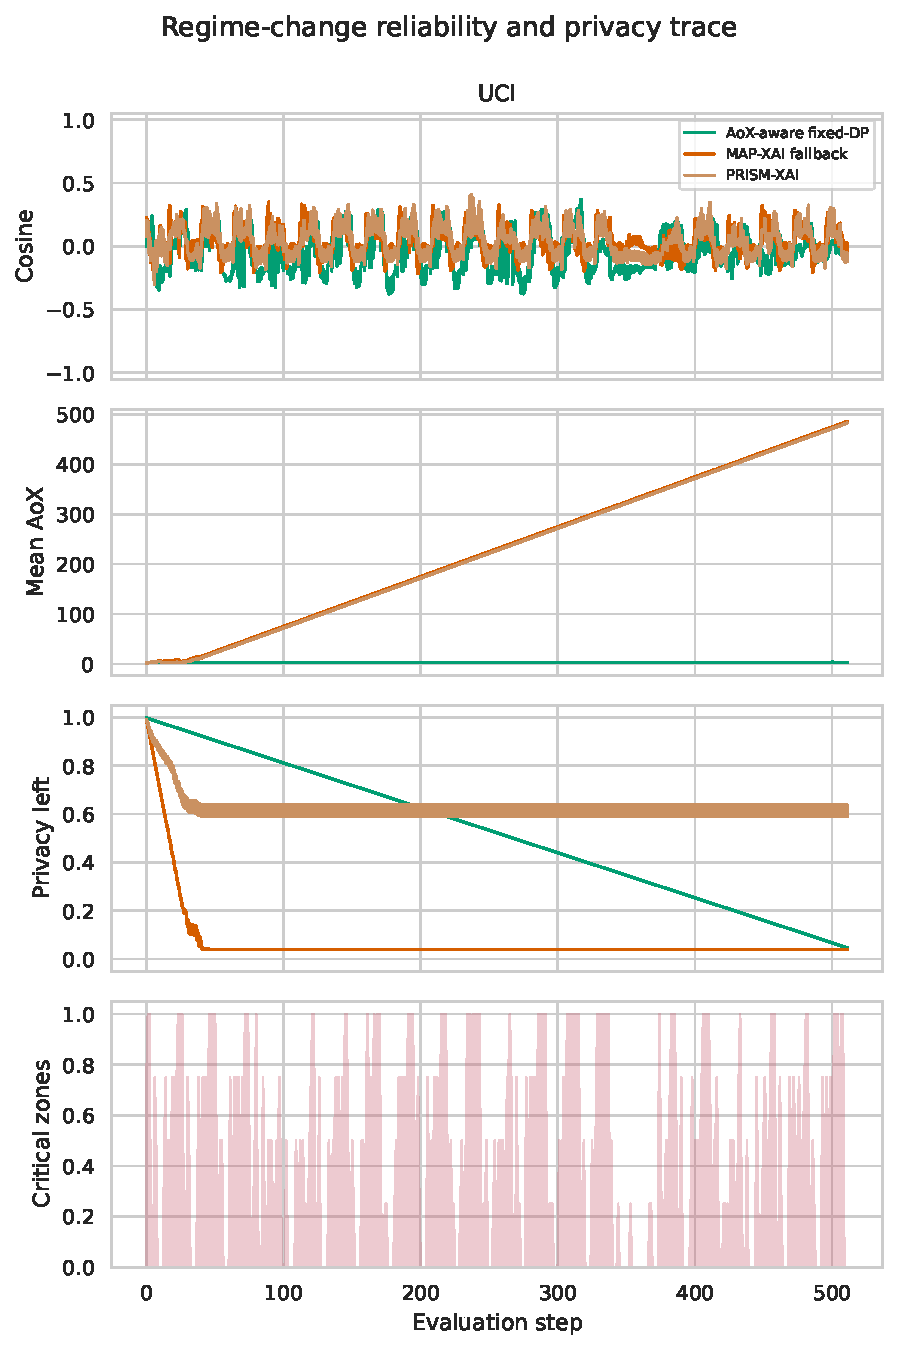
\includegraphics[width=.96\textwidth,height=.82\textheight,keepaspectratio]{../../SERVICE_TRADEOFF_RESULTS/runs/thr_1_cap_32/uci/regime_trace.pdf}

\caption{Public-score threshold $\tau=1$, release cap $M=32$, UCI: representative regime trace. This panel should be read with the setting-level quantitative interpretation and the complete tables immediately preceding the figure block.}

\end{figure*}

\clearpage

\begin{figure*}[p]

\centering

\includegraphics[width=.96\textwidth,height=.82\textheight,keepaspectratio]{../../SERVICE_TRADEOFF_RESULTS/runs/thr_1_cap_32/uci/fairness_reliability.pdf}

\caption{Public-score threshold $\tau=1$, release cap $M=32$, UCI: fairness--reliability plane. This panel should be read with the setting-level quantitative interpretation and the complete tables immediately preceding the figure block.}

\end{figure*}

\clearpage

\begin{figure*}[p]

\centering

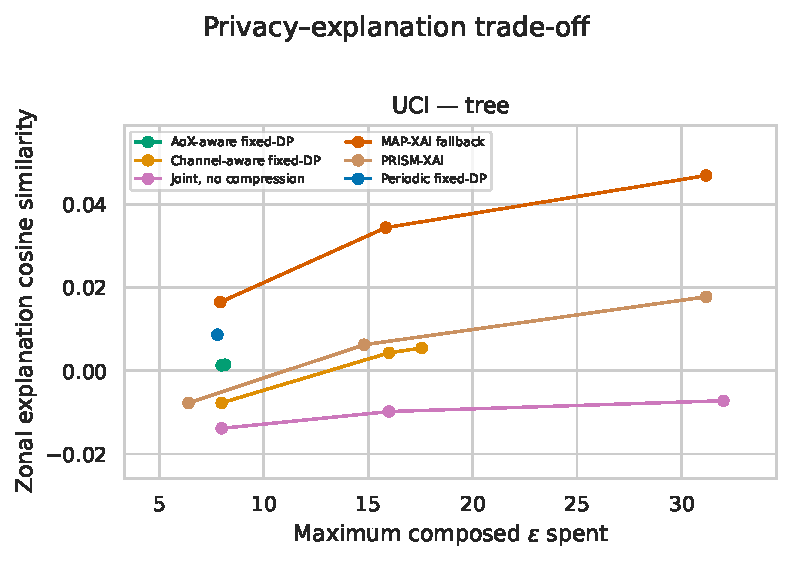
\includegraphics[width=.96\textwidth,height=.82\textheight,keepaspectratio]{../../SERVICE_TRADEOFF_RESULTS/runs/thr_1_cap_32/uci/privacy_fidelity.pdf}

\caption{Public-score threshold $\tau=1$, release cap $M=32$, UCI: privacy--fidelity plane. This panel should be read with the setting-level quantitative interpretation and the complete tables immediately preceding the figure block.}

\end{figure*}

\clearpage

\begin{figure*}[p]

\centering

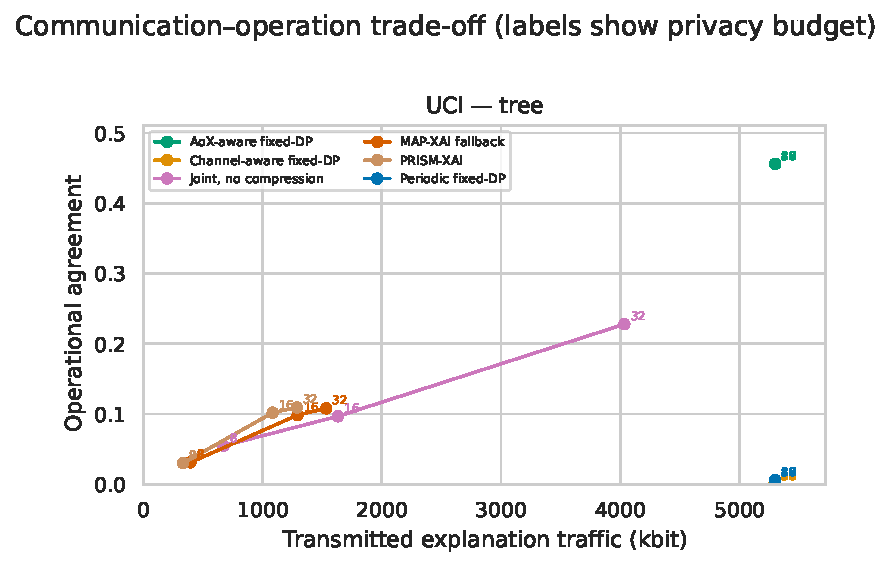
\includegraphics[width=.96\textwidth,height=.82\textheight,keepaspectratio]{../../SERVICE_TRADEOFF_RESULTS/runs/thr_1_cap_32/uci/pareto_bits_fidelity.pdf}

\caption{Public-score threshold $\tau=1$, release cap $M=32$, UCI: traffic--fidelity Pareto plane. This panel should be read with the setting-level quantitative interpretation and the complete tables immediately preceding the figure block.}

\end{figure*}

\clearpage

\begin{figure*}[p]

\centering

\includegraphics[width=.96\textwidth,height=.82\textheight,keepaspectratio]{../../SERVICE_TRADEOFF_RESULTS/runs/thr_1_cap_32/uci/ablation_results.pdf}

\caption{Public-score threshold $\tau=1$, release cap $M=32$, UCI: component ablation. This panel should be read with the setting-level quantitative interpretation and the complete tables immediately preceding the figure block.}

\end{figure*}

\clearpage

\subsubsection{Public-score threshold $\tau=3$, release cap $M=32$}

At this operating point, PRISM-XAI transmits 584.33~kbit versus 688.42~kbit for MAP-XAI-only (aggregate-mean ratio saving 15.12\%). The paired difference is -104.09$\pm$13.56~kbit. PRISM coverage is 0.2064, critical-event recall is 0.0852, and maximum recorded expenditure is 17.301. Relative to MAP-XAI-only, the paired coverage change is -0.00010$\pm$0.00026 and recall change is +0.00124$\pm$0.00307. The descriptive overlap rule holds in 5 of 12 cells. Accordingly, this point is read as a sensitivity point on the service frontier, not a complete matched-service confirmation.

\paragraph{Combined datasets.} The three generated tables below report the full method means, all condition-level values, and paired differences. The five figures that follow provide the corresponding temporal, fairness, privacy, Pareto, and ablation views. Aggregate panels support the setting-level summary above; dataset panels reveal whether that summary is shared by OPSD and UCI rather than being driven by their different endpoint counts.

\begin{table*}[p]\centering\tiny

\caption{Public-score threshold $\tau=3$, release cap $M=32$, Combined datasets: complete generated method table.}

\label{tab:thr_3_cap_32:combined:main}

\resizebox{\linewidth}{!}{% Values are means with 95% Student-t confidence intervals across seeds.
\begin{tabular}{lccccccccccccccc}
\toprule
Dataset & Model & $\epsilon_{\max}$ & Method & Top-$K$ & Cosine & Decision & Recall & Prec. & Abst. & P95 ms & kbit & Spent $\epsilon$ & False int. & bit/correct & Fairness \\
\midrule
OPSD & Tree & 8 & AoX-aware fixed-DP & 0.234 $\pm$ 0.048 & -0.033 $\pm$ 0.028 & 0.119 $\pm$ 0.028 & 0.119 $\pm$ 0.028 & 0.198 $\pm$ 0.054 & 0.721 $\pm$ 0.005 & 6.903 $\pm$ 1.126 & 1560.564 $\pm$ 0.000 & 7.990 $\pm$ 0.000 & 0.183 $\pm$ 0.020 & 35567.482 $\pm$ 10569.818 & 0.999 $\pm$ 0.000 \\
OPSD & Tree & 8 & AoX-aware fixed-DP & 0.238 $\pm$ 0.049 & -0.026 $\pm$ 0.055 & 0.121 $\pm$ 0.026 & 0.121 $\pm$ 0.026 & 0.205 $\pm$ 0.053 & 0.721 $\pm$ 0.005 & 6.903 $\pm$ 1.126 & 1560.564 $\pm$ 0.000 & 7.990 $\pm$ 0.000 & 0.179 $\pm$ 0.023 & 34123.214 $\pm$ 8376.542 & 0.999 $\pm$ 0.000 \\
OPSD & Tree & 8 & Channel-aware fixed-DP & 0.292 $\pm$ 0.037 & -0.041 $\pm$ 0.051 & 0.107 $\pm$ 0.026 & 0.107 $\pm$ 0.026 & 0.217 $\pm$ 0.068 & 0.779 $\pm$ 0.011 & 5.571 $\pm$ 1.784 & 1560.564 $\pm$ 0.000 & 7.990 $\pm$ 0.000 & 0.154 $\pm$ 0.029 & 40860.756 $\pm$ 14126.920 & 0.999 $\pm$ 0.000 \\
OPSD & Tree & 8 & Channel-aware fixed-DP & 0.292 $\pm$ 0.054 & -0.049 $\pm$ 0.064 & 0.111 $\pm$ 0.023 & 0.111 $\pm$ 0.023 & 0.228 $\pm$ 0.066 & 0.779 $\pm$ 0.011 & 5.571 $\pm$ 1.784 & 1560.564 $\pm$ 0.000 & 7.990 $\pm$ 0.000 & 0.149 $\pm$ 0.026 & 37980.855 $\pm$ 12338.094 & 0.999 $\pm$ 0.000 \\
OPSD & Tree & 8 & Joint, no compression & 0.288 $\pm$ 0.064 & -0.030 $\pm$ 0.079 & 0.016 $\pm$ 0.005 & 0.016 $\pm$ 0.005 & 0.193 $\pm$ 0.059 & 0.957 $\pm$ 0.003 & 4.560 $\pm$ 1.811 & 189.900 $\pm$ 0.554 & 7.990 $\pm$ 0.000 & 0.027 $\pm$ 0.005 & 32490.357 $\pm$ 10149.755 & 0.996 $\pm$ 0.002 \\
OPSD & Tree & 8 & Joint, no compression & 0.258 $\pm$ 0.055 & 0.011 $\pm$ 0.094 & 0.019 $\pm$ 0.004 & 0.019 $\pm$ 0.004 & 0.224 $\pm$ 0.044 & 0.957 $\pm$ 0.003 & 4.562 $\pm$ 1.809 & 189.750 $\pm$ 0.566 & 7.990 $\pm$ 0.000 & 0.025 $\pm$ 0.003 & 26079.167 $\pm$ 6335.386 & 0.996 $\pm$ 0.002 \\
OPSD & Tree & 8 & Periodic fixed-DP & 0.241 $\pm$ 0.049 & -0.019 $\pm$ 0.061 & 0.125 $\pm$ 0.020 & 0.125 $\pm$ 0.020 & 0.209 $\pm$ 0.044 & 0.722 $\pm$ 0.006 & 6.303 $\pm$ 1.438 & 1560.564 $\pm$ 0.000 & 7.990 $\pm$ 0.000 & 0.181 $\pm$ 0.021 & 31183.082 $\pm$ 4356.378 & 0.999 $\pm$ 0.000 \\
OPSD & Tree & 8 & Periodic fixed-DP & 0.242 $\pm$ 0.048 & -0.026 $\pm$ 0.082 & 0.135 $\pm$ 0.016 & 0.135 $\pm$ 0.016 & 0.231 $\pm$ 0.037 & 0.722 $\pm$ 0.006 & 6.303 $\pm$ 1.438 & 1560.564 $\pm$ 0.000 & 7.990 $\pm$ 0.000 & 0.169 $\pm$ 0.017 & 28520.235 $\pm$ 3511.595 & 0.999 $\pm$ 0.000 \\
OPSD & Tree & 8 & PRISM-XAI & 0.257 $\pm$ 0.067 & 0.028 $\pm$ 0.059 & 0.028 $\pm$ 0.011 & 0.028 $\pm$ 0.011 & 0.273 $\pm$ 0.131 & 0.923 $\pm$ 0.004 & 4.713 $\pm$ 1.733 & 96.298 $\pm$ 1.228 & 5.340 $\pm$ 0.419 & 0.030 $\pm$ 0.007 & 11906.519 $\pm$ 6206.672 & 0.989 $\pm$ 0.004 \\
OPSD & Tree & 8 & PRISM-XAI & 0.220 $\pm$ 0.047 & 0.027 $\pm$ 0.062 & 0.029 $\pm$ 0.013 & 0.029 $\pm$ 0.013 & 0.278 $\pm$ 0.137 & 0.923 $\pm$ 0.004 & 4.708 $\pm$ 1.737 & 95.592 $\pm$ 1.248 & 5.012 $\pm$ 0.388 & 0.030 $\pm$ 0.007 & 13471.090 $\pm$ 9725.652 & 0.989 $\pm$ 0.004 \\
OPSD & Tree & 8 & MAP-XAI fallback & 0.240 $\pm$ 0.060 & 0.022 $\pm$ 0.057 & 0.030 $\pm$ 0.008 & 0.030 $\pm$ 0.008 & 0.271 $\pm$ 0.091 & 0.923 $\pm$ 0.004 & 4.795 $\pm$ 1.684 & 115.748 $\pm$ 1.149 & 7.924 $\pm$ 0.000 & 0.031 $\pm$ 0.006 & 10380.916 $\pm$ 2295.453 & 0.989 $\pm$ 0.004 \\
OPSD & Tree & 8 & MAP-XAI fallback & 0.242 $\pm$ 0.055 & 0.038 $\pm$ 0.059 & 0.028 $\pm$ 0.007 & 0.028 $\pm$ 0.007 & 0.248 $\pm$ 0.070 & 0.923 $\pm$ 0.004 & 4.795 $\pm$ 1.684 & 115.607 $\pm$ 1.156 & 7.924 $\pm$ 0.000 & 0.032 $\pm$ 0.005 & 11185.765 $\pm$ 2730.237 & 0.989 $\pm$ 0.004 \\
UCI & Tree & 8 & AoX-aware fixed-DP & 0.263 $\pm$ 0.041 & -0.007 $\pm$ 0.009 & 0.457 $\pm$ 0.031 & 0.457 $\pm$ 0.031 & 0.362 $\pm$ 0.024 & 0.003 $\pm$ 0.001 & 7.500 $\pm$ 0.000 & 5300.224 $\pm$ 0.000 & 7.990 $\pm$ 0.000 & 0.557 $\pm$ 0.025 & 14002.896 $\pm$ 1040.243 & 0.999 $\pm$ 0.000 \\
UCI & Tree & 8 & AoX-aware fixed-DP & 0.260 $\pm$ 0.022 & 0.010 $\pm$ 0.055 & 0.455 $\pm$ 0.047 & 0.455 $\pm$ 0.047 & 0.361 $\pm$ 0.038 & 0.003 $\pm$ 0.001 & 7.500 $\pm$ 0.000 & 5300.224 $\pm$ 0.000 & 7.990 $\pm$ 0.000 & 0.557 $\pm$ 0.048 & 14198.303 $\pm$ 1508.274 & 0.999 $\pm$ 0.000 \\
UCI & Tree & 8 & Channel-aware fixed-DP & 0.248 $\pm$ 0.031 & 0.004 $\pm$ 0.012 & 0.001 $\pm$ 0.001 & 0.001 $\pm$ 0.001 & 0.150 $\pm$ 0.151 & 0.999 $\pm$ 0.001 & 4.609 $\pm$ 1.781 & 5295.177 $\pm$ 3.740 & 7.990 $\pm$ 0.000 & 0.001 $\pm$ 0.001 & 4632196.500 $\pm$ 2102650.252 & 0.991 $\pm$ 0.001 \\
UCI & Tree & 8 & Channel-aware fixed-DP & 0.239 $\pm$ 0.030 & -0.020 $\pm$ 0.055 & 0.000 $\pm$ 0.000 & 0.000 $\pm$ 0.000 & 0.117 $\pm$ 0.225 & 0.999 $\pm$ 0.001 & 4.609 $\pm$ 1.781 & 5295.177 $\pm$ 3.740 & 7.990 $\pm$ 0.000 & 0.001 $\pm$ 0.001 & 5296989.000 $\pm$ 41104.572 & 0.991 $\pm$ 0.001 \\
UCI & Tree & 8 & Joint, no compression & 0.286 $\pm$ 0.045 & 0.004 $\pm$ 0.020 & 0.052 $\pm$ 0.005 & 0.052 $\pm$ 0.005 & 0.406 $\pm$ 0.037 & 0.875 $\pm$ 0.003 & 5.123 $\pm$ 1.792 & 672.300 $\pm$ 0.452 & 7.990 $\pm$ 0.000 & 0.053 $\pm$ 0.004 & 15676.175 $\pm$ 1475.621 & 0.994 $\pm$ 0.003 \\
UCI & Tree & 8 & Joint, no compression & 0.229 $\pm$ 0.052 & -0.032 $\pm$ 0.050 & 0.057 $\pm$ 0.007 & 0.057 $\pm$ 0.007 & 0.428 $\pm$ 0.041 & 0.875 $\pm$ 0.003 & 5.131 $\pm$ 1.787 & 672.300 $\pm$ 0.452 & 7.990 $\pm$ 0.000 & 0.052 $\pm$ 0.004 & 14702.786 $\pm$ 2334.488 & 0.994 $\pm$ 0.003 \\
UCI & Tree & 8 & Periodic fixed-DP & 0.259 $\pm$ 0.060 & -0.005 $\pm$ 0.008 & 0.006 $\pm$ 0.001 & 0.006 $\pm$ 0.001 & 0.244 $\pm$ 0.049 & 0.989 $\pm$ 0.001 & 4.596 $\pm$ 1.788 & 5299.318 $\pm$ 1.451 & 7.786 $\pm$ 0.000 & 0.013 $\pm$ 0.002 & 1215103.896 $\pm$ 390671.319 & 0.999 $\pm$ 0.000 \\
UCI & Tree & 8 & Periodic fixed-DP & 0.260 $\pm$ 0.044 & 0.022 $\pm$ 0.070 & 0.005 $\pm$ 0.001 & 0.005 $\pm$ 0.001 & 0.195 $\pm$ 0.050 & 0.989 $\pm$ 0.001 & 4.596 $\pm$ 1.788 & 5299.318 $\pm$ 1.451 & 7.786 $\pm$ 0.000 & 0.015 $\pm$ 0.002 & 1555837.203 $\pm$ 955472.503 & 0.999 $\pm$ 0.000 \\
UCI & Tree & 8 & PRISM-XAI & 0.207 $\pm$ 0.052 & 0.004 $\pm$ 0.012 & 0.046 $\pm$ 0.010 & 0.046 $\pm$ 0.010 & 0.469 $\pm$ 0.081 & 0.901 $\pm$ 0.005 & 5.035 $\pm$ 1.860 & 341.133 $\pm$ 1.293 & 6.779 $\pm$ 0.208 & 0.035 $\pm$ 0.005 & 9780.191 $\pm$ 2585.599 & 0.988 $\pm$ 0.003 \\
UCI & Tree & 8 & PRISM-XAI & 0.256 $\pm$ 0.043 & 0.000 $\pm$ 0.081 & 0.047 $\pm$ 0.008 & 0.047 $\pm$ 0.008 & 0.503 $\pm$ 0.086 & 0.902 $\pm$ 0.005 & 5.524 $\pm$ 1.825 & 338.064 $\pm$ 2.047 & 6.657 $\pm$ 0.214 & 0.032 $\pm$ 0.007 & 9159.950 $\pm$ 1670.303 & 0.989 $\pm$ 0.003 \\
UCI & Tree & 8 & MAP-XAI fallback & 0.193 $\pm$ 0.046 & 0.014 $\pm$ 0.010 & 0.046 $\pm$ 0.007 & 0.046 $\pm$ 0.007 & 0.479 $\pm$ 0.053 & 0.901 $\pm$ 0.005 & 5.106 $\pm$ 1.806 & 395.052 $\pm$ 0.314 & 7.924 $\pm$ 0.000 & 0.035 $\pm$ 0.004 & 10596.392 $\pm$ 1554.907 & 0.988 $\pm$ 0.003 \\
UCI & Tree & 8 & MAP-XAI fallback & 0.246 $\pm$ 0.061 & 0.064 $\pm$ 0.067 & 0.049 $\pm$ 0.007 & 0.049 $\pm$ 0.007 & 0.510 $\pm$ 0.076 & 0.902 $\pm$ 0.005 & 5.409 $\pm$ 1.720 & 395.226 $\pm$ 1.353 & 7.924 $\pm$ 0.000 & 0.033 $\pm$ 0.007 & 10216.728 $\pm$ 2063.280 & 0.989 $\pm$ 0.003 \\
\bottomrule
\end{tabular}
}

\end{table*}\clearpage

\begin{table*}[p]\centering\tiny

\caption{Public-score threshold $\tau=3$, release cap $M=32$, Combined datasets: complete condition-level generated table.}

\label{tab:thr_3_cap_32:combined:conditions}

\resizebox{\textwidth}{!}{\begin{tabular}{llllccccccccccc}
\toprule
Dataset & Model & $\epsilon_{\max}$ & Method & kbit & Top-$K$ & Random Top-$K$ & Cosine & Decision & Recall & Precision & Coverage & Abstain & False int. & Spent $\epsilon$ \\
\midrule
OPSD & Tree & 8 & Joint, no compression & 189.900 $\pm$ 0.554 & 0.288 $\pm$ 0.064 & 0.250 $\pm$ 0.000 & -0.030 $\pm$ 0.079 & 0.016 $\pm$ 0.005 & 0.016 $\pm$ 0.005 & 0.193 $\pm$ 0.059 & 0.043 $\pm$ 0.003 & 0.957 $\pm$ 0.003 & 0.027 $\pm$ 0.005 & 7.990 $\pm$ 0.000 \\
OPSD & Tree & 8 & Joint, no compression & 189.750 $\pm$ 0.566 & 0.258 $\pm$ 0.055 & 0.250 $\pm$ 0.000 & 0.011 $\pm$ 0.094 & 0.019 $\pm$ 0.004 & 0.019 $\pm$ 0.004 & 0.224 $\pm$ 0.044 & 0.043 $\pm$ 0.003 & 0.957 $\pm$ 0.003 & 0.025 $\pm$ 0.003 & 7.990 $\pm$ 0.000 \\
OPSD & Tree & 8 & Periodic fixed-DP & 1560.564 $\pm$ 0.000 & 0.241 $\pm$ 0.049 & 0.250 $\pm$ 0.000 & -0.019 $\pm$ 0.061 & 0.125 $\pm$ 0.020 & 0.125 $\pm$ 0.020 & 0.209 $\pm$ 0.044 & 0.278 $\pm$ 0.006 & 0.722 $\pm$ 0.006 & 0.181 $\pm$ 0.021 & 7.990 $\pm$ 0.000 \\
OPSD & Tree & 8 & Periodic fixed-DP & 1560.564 $\pm$ 0.000 & 0.242 $\pm$ 0.048 & 0.250 $\pm$ 0.000 & -0.026 $\pm$ 0.082 & 0.135 $\pm$ 0.016 & 0.135 $\pm$ 0.016 & 0.231 $\pm$ 0.037 & 0.278 $\pm$ 0.006 & 0.722 $\pm$ 0.006 & 0.169 $\pm$ 0.017 & 7.990 $\pm$ 0.000 \\
OPSD & Tree & 8 & PRISM-XAI & 96.298 $\pm$ 1.228 & 0.257 $\pm$ 0.067 & 0.250 $\pm$ 0.000 & 0.028 $\pm$ 0.059 & 0.028 $\pm$ 0.011 & 0.028 $\pm$ 0.011 & 0.273 $\pm$ 0.131 & 0.077 $\pm$ 0.004 & 0.923 $\pm$ 0.004 & 0.030 $\pm$ 0.007 & 5.340 $\pm$ 0.419 \\
OPSD & Tree & 8 & PRISM-XAI & 95.592 $\pm$ 1.248 & 0.220 $\pm$ 0.047 & 0.250 $\pm$ 0.000 & 0.027 $\pm$ 0.062 & 0.029 $\pm$ 0.013 & 0.029 $\pm$ 0.013 & 0.278 $\pm$ 0.137 & 0.077 $\pm$ 0.004 & 0.923 $\pm$ 0.004 & 0.030 $\pm$ 0.007 & 5.012 $\pm$ 0.388 \\
OPSD & Tree & 16 & Joint, no compression & 459.900 $\pm$ 0.750 & 0.232 $\pm$ 0.065 & 0.250 $\pm$ 0.000 & 0.059 $\pm$ 0.048 & 0.038 $\pm$ 0.009 & 0.038 $\pm$ 0.009 & 0.222 $\pm$ 0.049 & 0.088 $\pm$ 0.004 & 0.912 $\pm$ 0.004 & 0.049 $\pm$ 0.005 & 15.997 $\pm$ 0.000 \\
OPSD & Tree & 16 & Joint, no compression & 460.050 $\pm$ 0.724 & 0.241 $\pm$ 0.055 & 0.250 $\pm$ 0.000 & 0.061 $\pm$ 0.052 & 0.039 $\pm$ 0.008 & 0.039 $\pm$ 0.008 & 0.241 $\pm$ 0.042 & 0.088 $\pm$ 0.004 & 0.912 $\pm$ 0.004 & 0.045 $\pm$ 0.004 & 15.997 $\pm$ 0.000 \\
OPSD & Tree & 16 & Periodic fixed-DP & 5112.594 $\pm$ 0.000 & 0.249 $\pm$ 0.022 & 0.250 $\pm$ 0.000 & -0.009 $\pm$ 0.045 & 0.450 $\pm$ 0.062 & 0.450 $\pm$ 0.062 & 0.237 $\pm$ 0.042 & 0.985 $\pm$ 0.002 & 0.015 $\pm$ 0.002 & 0.551 $\pm$ 0.057 & 15.997 $\pm$ 0.000 \\
OPSD & Tree & 16 & Periodic fixed-DP & 5112.594 $\pm$ 0.000 & 0.243 $\pm$ 0.019 & 0.250 $\pm$ 0.000 & -0.012 $\pm$ 0.050 & 0.463 $\pm$ 0.047 & 0.463 $\pm$ 0.047 & 0.240 $\pm$ 0.028 & 0.985 $\pm$ 0.002 & 0.015 $\pm$ 0.002 & 0.547 $\pm$ 0.036 & 15.997 $\pm$ 0.000 \\
OPSD & Tree & 16 & PRISM-XAI & 300.705 $\pm$ 0.565 & 0.278 $\pm$ 0.056 & 0.250 $\pm$ 0.000 & 0.047 $\pm$ 0.080 & 0.066 $\pm$ 0.020 & 0.066 $\pm$ 0.020 & 0.224 $\pm$ 0.088 & 0.200 $\pm$ 0.005 & 0.800 $\pm$ 0.005 & 0.090 $\pm$ 0.015 & 14.564 $\pm$ 0.022 \\
OPSD & Tree & 16 & PRISM-XAI & 298.955 $\pm$ 0.657 & 0.289 $\pm$ 0.047 & 0.250 $\pm$ 0.000 & 0.055 $\pm$ 0.090 & 0.063 $\pm$ 0.021 & 0.063 $\pm$ 0.021 & 0.207 $\pm$ 0.090 & 0.199 $\pm$ 0.004 & 0.801 $\pm$ 0.004 & 0.097 $\pm$ 0.018 & 14.498 $\pm$ 0.044 \\
OPSD & Tree & 32 & Joint, no compression & 1140.900 $\pm$ 7.953 & 0.235 $\pm$ 0.064 & 0.250 $\pm$ 0.000 & -0.031 $\pm$ 0.089 & 0.074 $\pm$ 0.015 & 0.074 $\pm$ 0.015 & 0.205 $\pm$ 0.039 & 0.157 $\pm$ 0.006 & 0.843 $\pm$ 0.006 & 0.107 $\pm$ 0.009 & 31.999 $\pm$ 0.000 \\
OPSD & Tree & 32 & Joint, no compression & 1140.900 $\pm$ 7.953 & 0.282 $\pm$ 0.054 & 0.250 $\pm$ 0.000 & -0.044 $\pm$ 0.076 & 0.080 $\pm$ 0.011 & 0.080 $\pm$ 0.011 & 0.227 $\pm$ 0.052 & 0.158 $\pm$ 0.006 & 0.842 $\pm$ 0.006 & 0.105 $\pm$ 0.015 & 31.999 $\pm$ 0.000 \\
OPSD & Tree & 32 & Periodic fixed-DP & 5299.836 $\pm$ 0.625 & 0.249 $\pm$ 0.022 & 0.250 $\pm$ 0.000 & -0.009 $\pm$ 0.044 & 0.458 $\pm$ 0.066 & 0.458 $\pm$ 0.066 & 0.237 $\pm$ 0.045 & 1.000 $\pm$ 0.000 & 0.000 $\pm$ 0.000 & 0.562 $\pm$ 0.062 & 16.371 $\pm$ 0.000 \\
OPSD & Tree & 32 & Periodic fixed-DP & 5299.836 $\pm$ 0.625 & 0.244 $\pm$ 0.019 & 0.250 $\pm$ 0.000 & -0.012 $\pm$ 0.050 & 0.471 $\pm$ 0.049 & 0.471 $\pm$ 0.049 & 0.240 $\pm$ 0.029 & 1.000 $\pm$ 0.000 & 0.000 $\pm$ 0.000 & 0.559 $\pm$ 0.039 & 16.371 $\pm$ 0.000 \\
OPSD & Tree & 32 & PRISM-XAI & 356.570 $\pm$ 0.841 & 0.321 $\pm$ 0.068 & 0.250 $\pm$ 0.000 & 0.150 $\pm$ 0.077 & 0.105 $\pm$ 0.023 & 0.105 $\pm$ 0.023 & 0.301 $\pm$ 0.084 & 0.243 $\pm$ 0.007 & 0.757 $\pm$ 0.007 & 0.094 $\pm$ 0.017 & 31.175 $\pm$ 0.000 \\
OPSD & Tree & 32 & PRISM-XAI & 354.636 $\pm$ 0.782 & 0.326 $\pm$ 0.048 & 0.250 $\pm$ 0.000 & 0.146 $\pm$ 0.091 & 0.101 $\pm$ 0.022 & 0.101 $\pm$ 0.022 & 0.283 $\pm$ 0.077 & 0.243 $\pm$ 0.008 & 0.757 $\pm$ 0.008 & 0.099 $\pm$ 0.016 & 31.175 $\pm$ 0.000 \\
UCI & Tree & 8 & Joint, no compression & 672.300 $\pm$ 0.452 & 0.286 $\pm$ 0.045 & 0.250 $\pm$ 0.000 & 0.004 $\pm$ 0.020 & 0.052 $\pm$ 0.005 & 0.052 $\pm$ 0.005 & 0.406 $\pm$ 0.037 & 0.125 $\pm$ 0.003 & 0.875 $\pm$ 0.003 & 0.053 $\pm$ 0.004 & 7.990 $\pm$ 0.000 \\
UCI & Tree & 8 & Joint, no compression & 672.300 $\pm$ 0.452 & 0.229 $\pm$ 0.052 & 0.250 $\pm$ 0.000 & -0.032 $\pm$ 0.050 & 0.057 $\pm$ 0.007 & 0.057 $\pm$ 0.007 & 0.428 $\pm$ 0.041 & 0.125 $\pm$ 0.003 & 0.875 $\pm$ 0.003 & 0.052 $\pm$ 0.004 & 7.990 $\pm$ 0.000 \\
UCI & Tree & 8 & Periodic fixed-DP & 5299.318 $\pm$ 1.451 & 0.259 $\pm$ 0.060 & 0.250 $\pm$ 0.000 & -0.005 $\pm$ 0.008 & 0.006 $\pm$ 0.001 & 0.006 $\pm$ 0.001 & 0.244 $\pm$ 0.049 & 0.011 $\pm$ 0.001 & 0.989 $\pm$ 0.001 & 0.013 $\pm$ 0.002 & 7.786 $\pm$ 0.000 \\
UCI & Tree & 8 & Periodic fixed-DP & 5299.318 $\pm$ 1.451 & 0.260 $\pm$ 0.044 & 0.250 $\pm$ 0.000 & 0.022 $\pm$ 0.070 & 0.005 $\pm$ 0.001 & 0.005 $\pm$ 0.001 & 0.195 $\pm$ 0.050 & 0.011 $\pm$ 0.001 & 0.989 $\pm$ 0.001 & 0.015 $\pm$ 0.002 & 7.786 $\pm$ 0.000 \\
UCI & Tree & 8 & PRISM-XAI & 341.133 $\pm$ 1.293 & 0.207 $\pm$ 0.052 & 0.250 $\pm$ 0.000 & 0.004 $\pm$ 0.012 & 0.046 $\pm$ 0.010 & 0.046 $\pm$ 0.010 & 0.469 $\pm$ 0.081 & 0.099 $\pm$ 0.005 & 0.901 $\pm$ 0.005 & 0.035 $\pm$ 0.005 & 6.779 $\pm$ 0.208 \\
UCI & Tree & 8 & PRISM-XAI & 338.064 $\pm$ 2.047 & 0.256 $\pm$ 0.043 & 0.250 $\pm$ 0.000 & 0.000 $\pm$ 0.081 & 0.047 $\pm$ 0.008 & 0.047 $\pm$ 0.008 & 0.503 $\pm$ 0.086 & 0.098 $\pm$ 0.005 & 0.902 $\pm$ 0.005 & 0.032 $\pm$ 0.007 & 6.657 $\pm$ 0.214 \\
UCI & Tree & 16 & Joint, no compression & 1632.150 $\pm$ 0.339 & 0.216 $\pm$ 0.041 & 0.250 $\pm$ 0.000 & 0.001 $\pm$ 0.012 & 0.094 $\pm$ 0.005 & 0.094 $\pm$ 0.005 & 0.330 $\pm$ 0.024 & 0.228 $\pm$ 0.005 & 0.772 $\pm$ 0.005 & 0.133 $\pm$ 0.010 & 15.997 $\pm$ 0.000 \\
UCI & Tree & 16 & Joint, no compression & 1632.600 $\pm$ 0.554 & 0.204 $\pm$ 0.011 & 0.250 $\pm$ 0.000 & -0.021 $\pm$ 0.033 & 0.099 $\pm$ 0.016 & 0.099 $\pm$ 0.016 & 0.347 $\pm$ 0.054 & 0.228 $\pm$ 0.005 & 0.772 $\pm$ 0.005 & 0.128 $\pm$ 0.011 & 15.997 $\pm$ 0.000 \\
UCI & Tree & 16 & Periodic fixed-DP & 5299.318 $\pm$ 1.451 & 0.259 $\pm$ 0.060 & 0.250 $\pm$ 0.000 & -0.005 $\pm$ 0.008 & 0.006 $\pm$ 0.001 & 0.006 $\pm$ 0.001 & 0.244 $\pm$ 0.049 & 0.011 $\pm$ 0.001 & 0.989 $\pm$ 0.001 & 0.013 $\pm$ 0.002 & 7.786 $\pm$ 0.000 \\
UCI & Tree & 16 & Periodic fixed-DP & 5299.318 $\pm$ 1.451 & 0.260 $\pm$ 0.044 & 0.250 $\pm$ 0.000 & 0.022 $\pm$ 0.070 & 0.005 $\pm$ 0.001 & 0.005 $\pm$ 0.001 & 0.195 $\pm$ 0.050 & 0.011 $\pm$ 0.001 & 0.989 $\pm$ 0.001 & 0.015 $\pm$ 0.002 & 7.786 $\pm$ 0.000 \\
UCI & Tree & 16 & PRISM-XAI & 1110.802 $\pm$ 3.293 & 0.269 $\pm$ 0.046 & 0.250 $\pm$ 0.000 & 0.018 $\pm$ 0.010 & 0.126 $\pm$ 0.013 & 0.126 $\pm$ 0.013 & 0.407 $\pm$ 0.047 & 0.285 $\pm$ 0.006 & 0.715 $\pm$ 0.006 & 0.127 $\pm$ 0.012 & 15.063 $\pm$ 0.065 \\
UCI & Tree & 16 & PRISM-XAI & 1099.581 $\pm$ 2.815 & 0.240 $\pm$ 0.048 & 0.250 $\pm$ 0.000 & -0.063 $\pm$ 0.054 & 0.115 $\pm$ 0.016 & 0.115 $\pm$ 0.016 & 0.379 $\pm$ 0.064 & 0.282 $\pm$ 0.007 & 0.718 $\pm$ 0.007 & 0.132 $\pm$ 0.019 & 14.998 $\pm$ 0.062 \\
UCI & Tree & 32 & Joint, no compression & 4034.550 $\pm$ 5.034 & 0.246 $\pm$ 0.031 & 0.250 $\pm$ 0.000 & -0.002 $\pm$ 0.015 & 0.228 $\pm$ 0.013 & 0.228 $\pm$ 0.013 & 0.361 $\pm$ 0.028 & 0.537 $\pm$ 0.009 & 0.463 $\pm$ 0.009 & 0.279 $\pm$ 0.017 & 31.999 $\pm$ 0.000 \\
UCI & Tree & 32 & Joint, no compression & 4034.550 $\pm$ 5.034 & 0.241 $\pm$ 0.033 & 0.250 $\pm$ 0.000 & -0.012 $\pm$ 0.030 & 0.228 $\pm$ 0.028 & 0.228 $\pm$ 0.028 & 0.360 $\pm$ 0.047 & 0.530 $\pm$ 0.010 & 0.470 $\pm$ 0.010 & 0.280 $\pm$ 0.026 & 31.999 $\pm$ 0.000 \\
UCI & Tree & 32 & Periodic fixed-DP & 5299.318 $\pm$ 1.451 & 0.259 $\pm$ 0.060 & 0.250 $\pm$ 0.000 & -0.005 $\pm$ 0.008 & 0.006 $\pm$ 0.001 & 0.006 $\pm$ 0.001 & 0.244 $\pm$ 0.049 & 0.011 $\pm$ 0.001 & 0.989 $\pm$ 0.001 & 0.013 $\pm$ 0.002 & 7.786 $\pm$ 0.000 \\
UCI & Tree & 32 & Periodic fixed-DP & 5299.318 $\pm$ 1.451 & 0.260 $\pm$ 0.044 & 0.250 $\pm$ 0.000 & 0.022 $\pm$ 0.070 & 0.005 $\pm$ 0.001 & 0.005 $\pm$ 0.001 & 0.195 $\pm$ 0.050 & 0.011 $\pm$ 0.001 & 0.989 $\pm$ 0.001 & 0.015 $\pm$ 0.002 & 7.786 $\pm$ 0.000 \\
UCI & Tree & 32 & PRISM-XAI & 1317.135 $\pm$ 2.878 & 0.286 $\pm$ 0.041 & 0.250 $\pm$ 0.000 & 0.016 $\pm$ 0.014 & 0.150 $\pm$ 0.019 & 0.150 $\pm$ 0.019 & 0.423 $\pm$ 0.062 & 0.338 $\pm$ 0.007 & 0.662 $\pm$ 0.007 & 0.143 $\pm$ 0.016 & 31.175 $\pm$ 0.000 \\
UCI & Tree & 32 & PRISM-XAI & 1302.454 $\pm$ 3.178 & 0.249 $\pm$ 0.044 & 0.250 $\pm$ 0.000 & -0.087 $\pm$ 0.048 & 0.148 $\pm$ 0.011 & 0.148 $\pm$ 0.011 & 0.437 $\pm$ 0.045 & 0.335 $\pm$ 0.007 & 0.665 $\pm$ 0.007 & 0.132 $\pm$ 0.013 & 31.175 $\pm$ 0.000 \\
\bottomrule
\end{tabular}
}

\end{table*}\clearpage

\begin{table*}[p]\centering\tiny

\caption{Public-score threshold $\tau=3$, release cap $M=32$, Combined datasets: complete generated paired comparisons.}

\label{tab:thr_3_cap_32:combined:paired}

\resizebox{\textwidth}{!}{\begin{tabular}{llcccc}
\toprule
Dataset & Baseline & Delta kbit & Delta Top-$K$ & Delta recall & Delta fairness \\
\midrule
OPSD & AoX-aware fixed-DP & -1464.266 $\pm$ 1.228 & 0.024 $\pm$ 0.053 & -0.092 $\pm$ 0.036 & -0.010 $\pm$ 0.004 \\
OPSD & AoX-aware fixed-DP & -4799.207 $\pm$ 5.399 & 0.025 $\pm$ 0.072 & -0.335 $\pm$ 0.087 & -0.002 $\pm$ 0.001 \\
OPSD & AoX-aware fixed-DP & -4943.654 $\pm$ 0.841 & 0.068 $\pm$ 0.080 & -0.308 $\pm$ 0.086 & -0.002 $\pm$ 0.001 \\
OPSD & AoX-aware fixed-DP & -1464.972 $\pm$ 1.248 & -0.018 $\pm$ 0.064 & -0.092 $\pm$ 0.035 & -0.010 $\pm$ 0.004 \\
OPSD & AoX-aware fixed-DP & -4800.957 $\pm$ 5.327 & 0.036 $\pm$ 0.052 & -0.351 $\pm$ 0.071 & -0.002 $\pm$ 0.001 \\
OPSD & AoX-aware fixed-DP & -4945.588 $\pm$ 0.782 & 0.074 $\pm$ 0.055 & -0.325 $\pm$ 0.067 & -0.002 $\pm$ 0.001 \\
OPSD & Channel-aware fixed-DP & -1464.266 $\pm$ 1.228 & -0.035 $\pm$ 0.061 & -0.079 $\pm$ 0.032 & -0.010 $\pm$ 0.004 \\
OPSD & Channel-aware fixed-DP & -4385.904 $\pm$ 13.238 & 0.016 $\pm$ 0.064 & -0.335 $\pm$ 0.100 & 0.060 $\pm$ 0.005 \\
OPSD & Channel-aware fixed-DP & -4943.654 $\pm$ 0.841 & 0.063 $\pm$ 0.076 & -0.330 $\pm$ 0.104 & 0.091 $\pm$ 0.005 \\
OPSD & Channel-aware fixed-DP & -1464.972 $\pm$ 1.248 & -0.072 $\pm$ 0.074 & -0.082 $\pm$ 0.031 & -0.010 $\pm$ 0.004 \\
OPSD & Channel-aware fixed-DP & -4387.654 $\pm$ 13.405 & 0.031 $\pm$ 0.047 & -0.356 $\pm$ 0.098 & 0.060 $\pm$ 0.005 \\
OPSD & Channel-aware fixed-DP & -4945.588 $\pm$ 0.782 & 0.069 $\pm$ 0.051 & -0.355 $\pm$ 0.094 & 0.091 $\pm$ 0.005 \\
OPSD & Joint, no compression & -93.602 $\pm$ 1.154 & -0.031 $\pm$ 0.103 & 0.011 $\pm$ 0.012 & -0.007 $\pm$ 0.004 \\
OPSD & Joint, no compression & -159.195 $\pm$ 1.122 & 0.047 $\pm$ 0.099 & 0.028 $\pm$ 0.023 & 0.000 $\pm$ 0.001 \\
OPSD & Joint, no compression & -784.330 $\pm$ 7.944 & 0.086 $\pm$ 0.101 & 0.031 $\pm$ 0.032 & -0.001 $\pm$ 0.001 \\
OPSD & Joint, no compression & -94.158 $\pm$ 1.241 & -0.038 $\pm$ 0.069 & 0.010 $\pm$ 0.013 & -0.007 $\pm$ 0.004 \\
OPSD & Joint, no compression & -161.095 $\pm$ 1.115 & 0.048 $\pm$ 0.086 & 0.025 $\pm$ 0.021 & 0.000 $\pm$ 0.001 \\
OPSD & Joint, no compression & -786.264 $\pm$ 8.092 & 0.044 $\pm$ 0.080 & 0.021 $\pm$ 0.024 & -0.001 $\pm$ 0.001 \\
OPSD & Periodic fixed-DP & -1464.266 $\pm$ 1.228 & 0.017 $\pm$ 0.044 & -0.097 $\pm$ 0.025 & -0.010 $\pm$ 0.004 \\
OPSD & Periodic fixed-DP & -4811.889 $\pm$ 0.565 & 0.029 $\pm$ 0.053 & -0.384 $\pm$ 0.072 & -0.002 $\pm$ 0.001 \\
OPSD & Periodic fixed-DP & -4943.266 $\pm$ 0.807 & 0.072 $\pm$ 0.074 & -0.353 $\pm$ 0.071 & -0.002 $\pm$ 0.001 \\
OPSD & Periodic fixed-DP & -1464.972 $\pm$ 1.248 & -0.022 $\pm$ 0.054 & -0.106 $\pm$ 0.022 & -0.010 $\pm$ 0.004 \\
OPSD & Periodic fixed-DP & -4813.639 $\pm$ 0.657 & 0.046 $\pm$ 0.040 & -0.399 $\pm$ 0.060 & -0.002 $\pm$ 0.001 \\
OPSD & Periodic fixed-DP & -4945.200 $\pm$ 0.800 & 0.082 $\pm$ 0.043 & -0.370 $\pm$ 0.053 & -0.002 $\pm$ 0.001 \\
OPSD & MAP-XAI fallback & -19.450 $\pm$ 0.713 & 0.017 $\pm$ 0.052 & -0.002 $\pm$ 0.006 & 0.000 $\pm$ 0.000 \\
OPSD & MAP-XAI fallback & -62.093 $\pm$ 0.598 & -0.013 $\pm$ 0.032 & 0.003 $\pm$ 0.015 & 0.000 $\pm$ 0.000 \\
OPSD & MAP-XAI fallback & -73.728 $\pm$ 0.773 & -0.007 $\pm$ 0.048 & 0.011 $\pm$ 0.016 & 0.000 $\pm$ 0.000 \\
OPSD & MAP-XAI fallback & -20.015 $\pm$ 0.643 & -0.022 $\pm$ 0.056 & 0.001 $\pm$ 0.007 & 0.000 $\pm$ 0.000 \\
OPSD & MAP-XAI fallback & -63.701 $\pm$ 0.679 & -0.004 $\pm$ 0.046 & -0.001 $\pm$ 0.018 & 0.000 $\pm$ 0.000 \\
OPSD & MAP-XAI fallback & -75.500 $\pm$ 0.722 & 0.005 $\pm$ 0.038 & 0.012 $\pm$ 0.013 & 0.000 $\pm$ 0.000 \\
UCI & AoX-aware fixed-DP & -4959.091 $\pm$ 1.293 & -0.056 $\pm$ 0.063 & -0.411 $\pm$ 0.026 & -0.011 $\pm$ 0.003 \\
UCI & AoX-aware fixed-DP & -4189.422 $\pm$ 3.293 & 0.005 $\pm$ 0.058 & -0.332 $\pm$ 0.035 & -0.002 $\pm$ 0.001 \\
UCI & AoX-aware fixed-DP & -3983.089 $\pm$ 2.878 & 0.023 $\pm$ 0.064 & -0.307 $\pm$ 0.043 & -0.001 $\pm$ 0.001 \\
UCI & AoX-aware fixed-DP & -4962.160 $\pm$ 2.047 & -0.004 $\pm$ 0.042 & -0.409 $\pm$ 0.046 & -0.010 $\pm$ 0.003 \\
UCI & AoX-aware fixed-DP & -4200.643 $\pm$ 2.815 & -0.020 $\pm$ 0.050 & -0.340 $\pm$ 0.048 & -0.002 $\pm$ 0.001 \\
UCI & AoX-aware fixed-DP & -3997.770 $\pm$ 3.178 & -0.012 $\pm$ 0.032 & -0.307 $\pm$ 0.052 & -0.001 $\pm$ 0.001 \\
UCI & Channel-aware fixed-DP & -4954.044 $\pm$ 4.047 & -0.041 $\pm$ 0.066 & 0.046 $\pm$ 0.010 & -0.002 $\pm$ 0.003 \\
UCI & Channel-aware fixed-DP & -4189.422 $\pm$ 3.293 & 0.001 $\pm$ 0.058 & 0.125 $\pm$ 0.013 & 0.667 $\pm$ 0.001 \\
UCI & Channel-aware fixed-DP & -3983.089 $\pm$ 2.878 & 0.018 $\pm$ 0.049 & 0.150 $\pm$ 0.019 & 0.743 $\pm$ 0.001 \\
UCI & Channel-aware fixed-DP & -4957.113 $\pm$ 4.745 & 0.017 $\pm$ 0.045 & 0.046 $\pm$ 0.008 & -0.002 $\pm$ 0.003 \\
UCI & Channel-aware fixed-DP & -4200.643 $\pm$ 2.815 & -0.020 $\pm$ 0.052 & 0.115 $\pm$ 0.016 & 0.667 $\pm$ 0.001 \\
UCI & Channel-aware fixed-DP & -3997.770 $\pm$ 3.178 & -0.011 $\pm$ 0.043 & 0.148 $\pm$ 0.011 & 0.743 $\pm$ 0.001 \\
UCI & Joint, no compression & -331.167 $\pm$ 1.523 & -0.079 $\pm$ 0.085 & -0.006 $\pm$ 0.011 & -0.006 $\pm$ 0.003 \\
UCI & Joint, no compression & -521.348 $\pm$ 3.369 & 0.052 $\pm$ 0.038 & 0.031 $\pm$ 0.015 & -0.000 $\pm$ 0.001 \\
UCI & Joint, no compression & -2717.415 $\pm$ 6.000 & 0.040 $\pm$ 0.049 & -0.077 $\pm$ 0.014 & -0.001 $\pm$ 0.001 \\
UCI & Joint, no compression & -334.236 $\pm$ 2.296 & 0.026 $\pm$ 0.066 & -0.010 $\pm$ 0.011 & -0.005 $\pm$ 0.003 \\
UCI & Joint, no compression & -533.019 $\pm$ 2.619 & 0.037 $\pm$ 0.048 & 0.016 $\pm$ 0.022 & -0.000 $\pm$ 0.001 \\
UCI & Joint, no compression & -2732.096 $\pm$ 5.519 & 0.007 $\pm$ 0.058 & -0.080 $\pm$ 0.032 & -0.001 $\pm$ 0.001 \\
UCI & Periodic fixed-DP & -4958.185 $\pm$ 2.040 & -0.053 $\pm$ 0.077 & 0.040 $\pm$ 0.010 & -0.011 $\pm$ 0.003 \\
UCI & Periodic fixed-DP & -4188.516 $\pm$ 3.590 & 0.009 $\pm$ 0.089 & 0.120 $\pm$ 0.014 & -0.002 $\pm$ 0.001 \\
UCI & Periodic fixed-DP & -3982.184 $\pm$ 3.108 & 0.027 $\pm$ 0.068 & 0.145 $\pm$ 0.020 & -0.002 $\pm$ 0.001 \\
UCI & Periodic fixed-DP & -4961.254 $\pm$ 2.973 & -0.005 $\pm$ 0.068 & 0.041 $\pm$ 0.007 & -0.011 $\pm$ 0.003 \\
UCI & Periodic fixed-DP & -4199.738 $\pm$ 3.048 & -0.020 $\pm$ 0.078 & 0.109 $\pm$ 0.015 & -0.002 $\pm$ 0.001 \\
UCI & Periodic fixed-DP & -3996.864 $\pm$ 3.261 & -0.012 $\pm$ 0.073 & 0.142 $\pm$ 0.011 & -0.002 $\pm$ 0.001 \\
UCI & MAP-XAI fallback & -53.919 $\pm$ 1.196 & 0.014 $\pm$ 0.036 & -0.000 $\pm$ 0.005 & 0.000 $\pm$ 0.000 \\
UCI & MAP-XAI fallback & -182.879 $\pm$ 3.287 & 0.006 $\pm$ 0.059 & -0.002 $\pm$ 0.010 & 0.000 $\pm$ 0.000 \\
UCI & MAP-XAI fallback & -216.465 $\pm$ 2.875 & 0.076 $\pm$ 0.044 & 0.002 $\pm$ 0.015 & 0.000 $\pm$ 0.000 \\
UCI & MAP-XAI fallback & -57.162 $\pm$ 1.160 & 0.010 $\pm$ 0.051 & -0.002 $\pm$ 0.008 & -0.000 $\pm$ 0.001 \\
UCI & MAP-XAI fallback & -193.593 $\pm$ 2.996 & 0.006 $\pm$ 0.034 & -0.010 $\pm$ 0.011 & -0.000 $\pm$ 0.000 \\
UCI & MAP-XAI fallback & -230.577 $\pm$ 3.247 & 0.018 $\pm$ 0.059 & 0.003 $\pm$ 0.011 & -0.000 $\pm$ 0.000 \\
\bottomrule
\end{tabular}
}

\end{table*}\clearpage

\begin{figure*}[p]

\centering

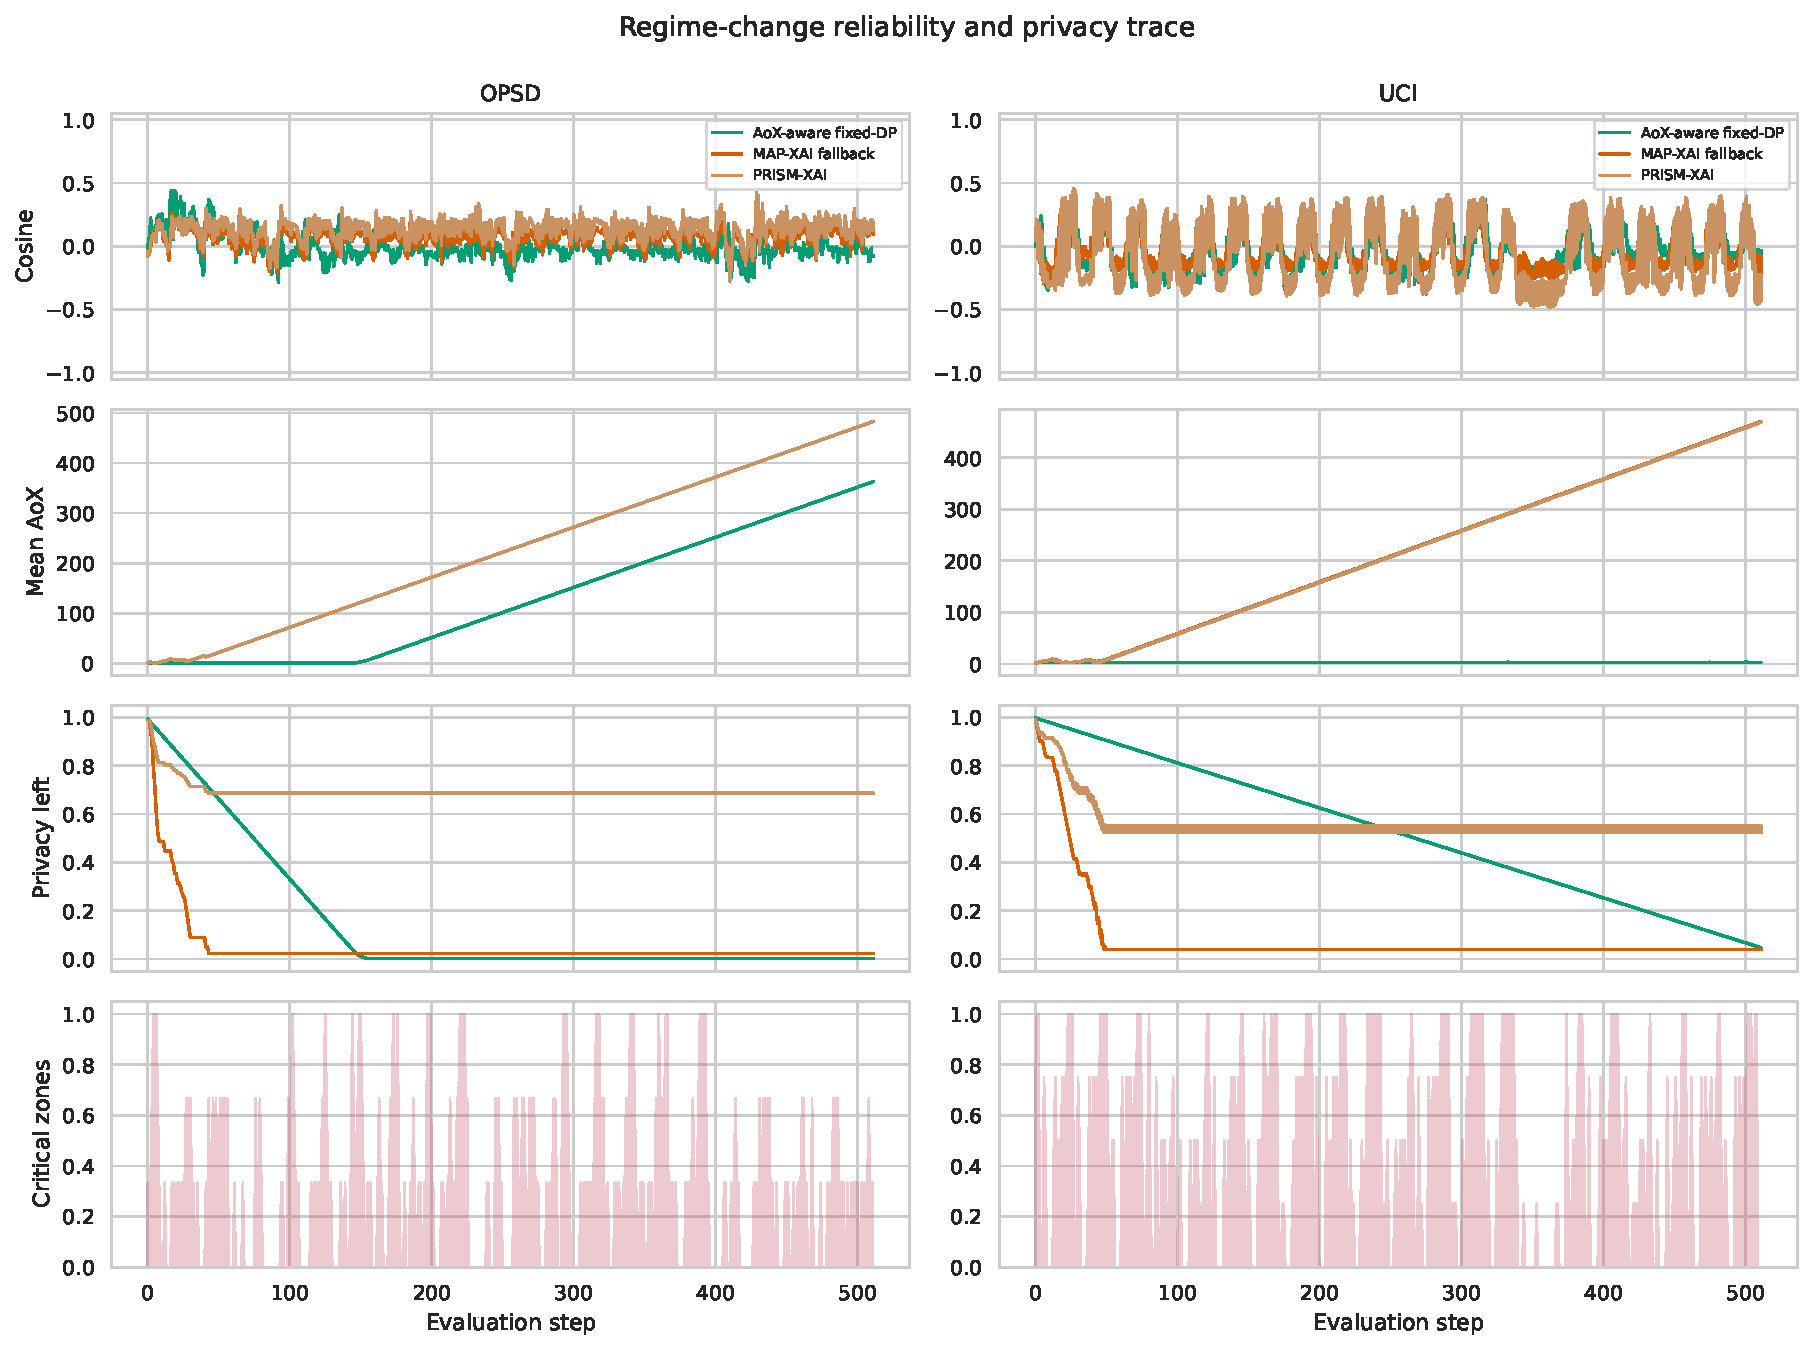
\includegraphics[width=.96\textwidth,height=.82\textheight,keepaspectratio]{../../SERVICE_TRADEOFF_RESULTS/runs/thr_3_cap_32/regime_trace.pdf}

\caption{Public-score threshold $\tau=3$, release cap $M=32$, Combined datasets: representative regime trace. This panel should be read with the setting-level quantitative interpretation and the complete tables immediately preceding the figure block.}

\end{figure*}

\clearpage

\begin{figure*}[p]

\centering

\includegraphics[width=.96\textwidth,height=.82\textheight,keepaspectratio]{../../SERVICE_TRADEOFF_RESULTS/runs/thr_3_cap_32/fairness_reliability.pdf}

\caption{Public-score threshold $\tau=3$, release cap $M=32$, Combined datasets: fairness--reliability plane. This panel should be read with the setting-level quantitative interpretation and the complete tables immediately preceding the figure block.}

\end{figure*}

\clearpage

\begin{figure*}[p]

\centering

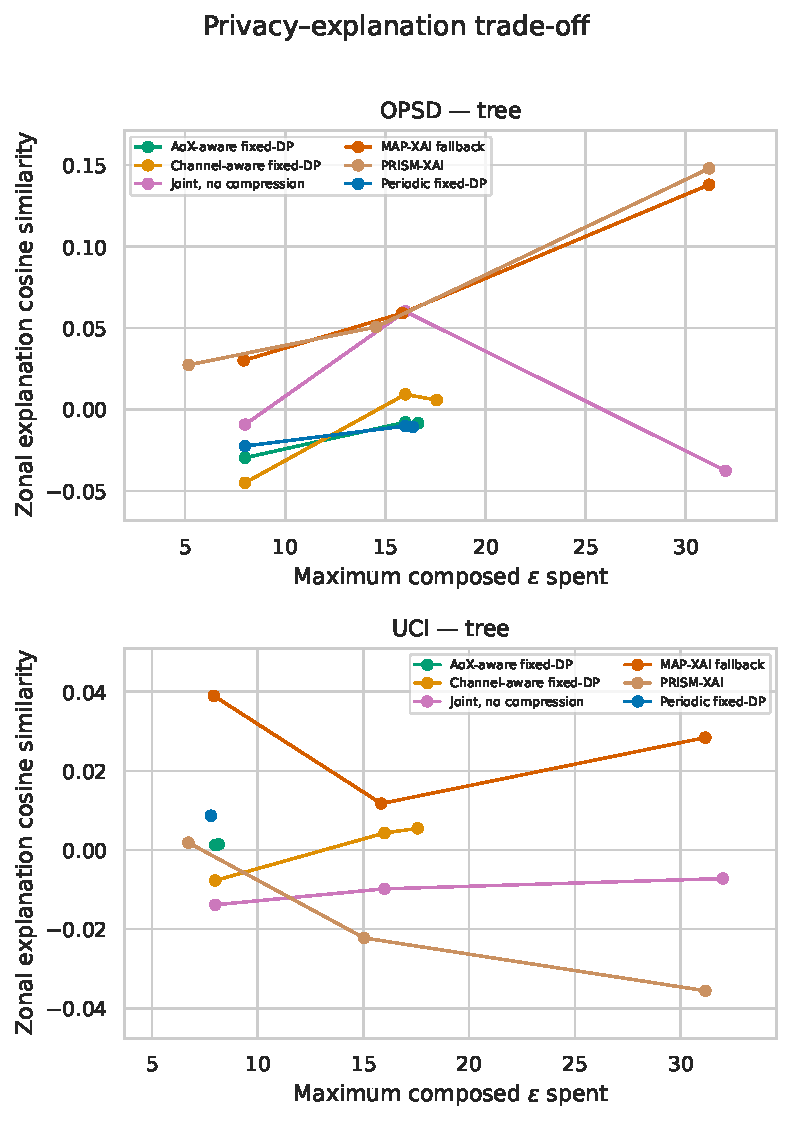
\includegraphics[width=.96\textwidth,height=.82\textheight,keepaspectratio]{../../SERVICE_TRADEOFF_RESULTS/runs/thr_3_cap_32/privacy_fidelity.pdf}

\caption{Public-score threshold $\tau=3$, release cap $M=32$, Combined datasets: privacy--fidelity plane. This panel should be read with the setting-level quantitative interpretation and the complete tables immediately preceding the figure block.}

\end{figure*}

\clearpage

\begin{figure*}[p]

\centering

\includegraphics[width=.96\textwidth,height=.82\textheight,keepaspectratio]{../../SERVICE_TRADEOFF_RESULTS/runs/thr_3_cap_32/pareto_bits_fidelity.pdf}

\caption{Public-score threshold $\tau=3$, release cap $M=32$, Combined datasets: traffic--fidelity Pareto plane. This panel should be read with the setting-level quantitative interpretation and the complete tables immediately preceding the figure block.}

\end{figure*}

\clearpage

\begin{figure*}[p]

\centering

\includegraphics[width=.96\textwidth,height=.82\textheight,keepaspectratio]{../../SERVICE_TRADEOFF_RESULTS/runs/thr_3_cap_32/ablation_results.pdf}

\caption{Public-score threshold $\tau=3$, release cap $M=32$, Combined datasets: component ablation. This panel should be read with the setting-level quantitative interpretation and the complete tables immediately preceding the figure block.}

\end{figure*}

\clearpage

\paragraph{OPSD.} The three generated tables below report the full method means, all condition-level values, and paired differences. The five figures that follow provide the corresponding temporal, fairness, privacy, Pareto, and ablation views. Aggregate panels support the setting-level summary above; dataset panels reveal whether that summary is shared by OPSD and UCI rather than being driven by their different endpoint counts.

\begin{table*}[p]\centering\tiny

\caption{Public-score threshold $\tau=3$, release cap $M=32$, OPSD: complete generated method table.}

\label{tab:thr_3_cap_32:opsd:main}

\resizebox{\linewidth}{!}{% Values are means with 95% Student-t confidence intervals across seeds.
\begin{tabular}{lccccccccccccccc}
\toprule
Dataset & Model & $\epsilon_{\max}$ & Method & Top-$K$ & Cosine & Decision & Recall & Prec. & Abst. & P95 ms & kbit & Spent $\epsilon$ & False int. & bit/correct & Fairness \\
\midrule
OPSD & Tree & 8 & AoX-aware fixed-DP & 0.234 $\pm$ 0.048 & -0.033 $\pm$ 0.028 & 0.119 $\pm$ 0.028 & 0.119 $\pm$ 0.028 & 0.198 $\pm$ 0.054 & 0.721 $\pm$ 0.005 & 6.903 $\pm$ 1.126 & 1560.564 $\pm$ 0.000 & 7.990 $\pm$ 0.000 & 0.183 $\pm$ 0.020 & 35567.482 $\pm$ 10569.818 & 0.999 $\pm$ 0.000 \\
OPSD & Tree & 8 & AoX-aware fixed-DP & 0.238 $\pm$ 0.049 & -0.026 $\pm$ 0.055 & 0.121 $\pm$ 0.026 & 0.121 $\pm$ 0.026 & 0.205 $\pm$ 0.053 & 0.721 $\pm$ 0.005 & 6.903 $\pm$ 1.126 & 1560.564 $\pm$ 0.000 & 7.990 $\pm$ 0.000 & 0.179 $\pm$ 0.023 & 34123.214 $\pm$ 8376.542 & 0.999 $\pm$ 0.000 \\
OPSD & Tree & 8 & Channel-aware fixed-DP & 0.292 $\pm$ 0.037 & -0.041 $\pm$ 0.051 & 0.107 $\pm$ 0.026 & 0.107 $\pm$ 0.026 & 0.217 $\pm$ 0.068 & 0.779 $\pm$ 0.011 & 5.571 $\pm$ 1.784 & 1560.564 $\pm$ 0.000 & 7.990 $\pm$ 0.000 & 0.154 $\pm$ 0.029 & 40860.756 $\pm$ 14126.920 & 0.999 $\pm$ 0.000 \\
OPSD & Tree & 8 & Channel-aware fixed-DP & 0.292 $\pm$ 0.054 & -0.049 $\pm$ 0.064 & 0.111 $\pm$ 0.023 & 0.111 $\pm$ 0.023 & 0.228 $\pm$ 0.066 & 0.779 $\pm$ 0.011 & 5.571 $\pm$ 1.784 & 1560.564 $\pm$ 0.000 & 7.990 $\pm$ 0.000 & 0.149 $\pm$ 0.026 & 37980.855 $\pm$ 12338.094 & 0.999 $\pm$ 0.000 \\
OPSD & Tree & 8 & Joint, no compression & 0.288 $\pm$ 0.064 & -0.030 $\pm$ 0.079 & 0.016 $\pm$ 0.005 & 0.016 $\pm$ 0.005 & 0.193 $\pm$ 0.059 & 0.957 $\pm$ 0.003 & 4.560 $\pm$ 1.811 & 189.900 $\pm$ 0.554 & 7.990 $\pm$ 0.000 & 0.027 $\pm$ 0.005 & 32490.357 $\pm$ 10149.755 & 0.996 $\pm$ 0.002 \\
OPSD & Tree & 8 & Joint, no compression & 0.258 $\pm$ 0.055 & 0.011 $\pm$ 0.094 & 0.019 $\pm$ 0.004 & 0.019 $\pm$ 0.004 & 0.224 $\pm$ 0.044 & 0.957 $\pm$ 0.003 & 4.562 $\pm$ 1.809 & 189.750 $\pm$ 0.566 & 7.990 $\pm$ 0.000 & 0.025 $\pm$ 0.003 & 26079.167 $\pm$ 6335.386 & 0.996 $\pm$ 0.002 \\
OPSD & Tree & 8 & Periodic fixed-DP & 0.241 $\pm$ 0.049 & -0.019 $\pm$ 0.061 & 0.125 $\pm$ 0.020 & 0.125 $\pm$ 0.020 & 0.209 $\pm$ 0.044 & 0.722 $\pm$ 0.006 & 6.303 $\pm$ 1.438 & 1560.564 $\pm$ 0.000 & 7.990 $\pm$ 0.000 & 0.181 $\pm$ 0.021 & 31183.082 $\pm$ 4356.378 & 0.999 $\pm$ 0.000 \\
OPSD & Tree & 8 & Periodic fixed-DP & 0.242 $\pm$ 0.048 & -0.026 $\pm$ 0.082 & 0.135 $\pm$ 0.016 & 0.135 $\pm$ 0.016 & 0.231 $\pm$ 0.037 & 0.722 $\pm$ 0.006 & 6.303 $\pm$ 1.438 & 1560.564 $\pm$ 0.000 & 7.990 $\pm$ 0.000 & 0.169 $\pm$ 0.017 & 28520.235 $\pm$ 3511.595 & 0.999 $\pm$ 0.000 \\
OPSD & Tree & 8 & PRISM-XAI & 0.257 $\pm$ 0.067 & 0.028 $\pm$ 0.059 & 0.028 $\pm$ 0.011 & 0.028 $\pm$ 0.011 & 0.273 $\pm$ 0.131 & 0.923 $\pm$ 0.004 & 4.713 $\pm$ 1.733 & 96.298 $\pm$ 1.228 & 5.340 $\pm$ 0.419 & 0.030 $\pm$ 0.007 & 11906.519 $\pm$ 6206.672 & 0.989 $\pm$ 0.004 \\
OPSD & Tree & 8 & PRISM-XAI & 0.220 $\pm$ 0.047 & 0.027 $\pm$ 0.062 & 0.029 $\pm$ 0.013 & 0.029 $\pm$ 0.013 & 0.278 $\pm$ 0.137 & 0.923 $\pm$ 0.004 & 4.708 $\pm$ 1.737 & 95.592 $\pm$ 1.248 & 5.012 $\pm$ 0.388 & 0.030 $\pm$ 0.007 & 13471.090 $\pm$ 9725.652 & 0.989 $\pm$ 0.004 \\
OPSD & Tree & 8 & MAP-XAI fallback & 0.240 $\pm$ 0.060 & 0.022 $\pm$ 0.057 & 0.030 $\pm$ 0.008 & 0.030 $\pm$ 0.008 & 0.271 $\pm$ 0.091 & 0.923 $\pm$ 0.004 & 4.795 $\pm$ 1.684 & 115.748 $\pm$ 1.149 & 7.924 $\pm$ 0.000 & 0.031 $\pm$ 0.006 & 10380.916 $\pm$ 2295.453 & 0.989 $\pm$ 0.004 \\
OPSD & Tree & 8 & MAP-XAI fallback & 0.242 $\pm$ 0.055 & 0.038 $\pm$ 0.059 & 0.028 $\pm$ 0.007 & 0.028 $\pm$ 0.007 & 0.248 $\pm$ 0.070 & 0.923 $\pm$ 0.004 & 4.795 $\pm$ 1.684 & 115.607 $\pm$ 1.156 & 7.924 $\pm$ 0.000 & 0.032 $\pm$ 0.005 & 11185.765 $\pm$ 2730.237 & 0.989 $\pm$ 0.004 \\
\bottomrule
\end{tabular}
}

\end{table*}\clearpage

\begin{table*}[p]\centering\tiny

\caption{Public-score threshold $\tau=3$, release cap $M=32$, OPSD: complete condition-level generated table.}

\label{tab:thr_3_cap_32:opsd:conditions}

\resizebox{\textwidth}{!}{\begin{tabular}{llllccccccccccc}
\toprule
Dataset & Model & $\epsilon_{\max}$ & Method & kbit & Top-$K$ & Random Top-$K$ & Cosine & Decision & Recall & Precision & Coverage & Abstain & False int. & Spent $\epsilon$ \\
\midrule
OPSD & Tree & 8 & Joint, no compression & 189.900 $\pm$ 0.554 & 0.288 $\pm$ 0.064 & 0.250 $\pm$ 0.000 & -0.030 $\pm$ 0.079 & 0.016 $\pm$ 0.005 & 0.016 $\pm$ 0.005 & 0.193 $\pm$ 0.059 & 0.043 $\pm$ 0.003 & 0.957 $\pm$ 0.003 & 0.027 $\pm$ 0.005 & 7.990 $\pm$ 0.000 \\
OPSD & Tree & 8 & Joint, no compression & 189.750 $\pm$ 0.566 & 0.258 $\pm$ 0.055 & 0.250 $\pm$ 0.000 & 0.011 $\pm$ 0.094 & 0.019 $\pm$ 0.004 & 0.019 $\pm$ 0.004 & 0.224 $\pm$ 0.044 & 0.043 $\pm$ 0.003 & 0.957 $\pm$ 0.003 & 0.025 $\pm$ 0.003 & 7.990 $\pm$ 0.000 \\
OPSD & Tree & 8 & Periodic fixed-DP & 1560.564 $\pm$ 0.000 & 0.241 $\pm$ 0.049 & 0.250 $\pm$ 0.000 & -0.019 $\pm$ 0.061 & 0.125 $\pm$ 0.020 & 0.125 $\pm$ 0.020 & 0.209 $\pm$ 0.044 & 0.278 $\pm$ 0.006 & 0.722 $\pm$ 0.006 & 0.181 $\pm$ 0.021 & 7.990 $\pm$ 0.000 \\
OPSD & Tree & 8 & Periodic fixed-DP & 1560.564 $\pm$ 0.000 & 0.242 $\pm$ 0.048 & 0.250 $\pm$ 0.000 & -0.026 $\pm$ 0.082 & 0.135 $\pm$ 0.016 & 0.135 $\pm$ 0.016 & 0.231 $\pm$ 0.037 & 0.278 $\pm$ 0.006 & 0.722 $\pm$ 0.006 & 0.169 $\pm$ 0.017 & 7.990 $\pm$ 0.000 \\
OPSD & Tree & 8 & PRISM-XAI & 96.298 $\pm$ 1.228 & 0.257 $\pm$ 0.067 & 0.250 $\pm$ 0.000 & 0.028 $\pm$ 0.059 & 0.028 $\pm$ 0.011 & 0.028 $\pm$ 0.011 & 0.273 $\pm$ 0.131 & 0.077 $\pm$ 0.004 & 0.923 $\pm$ 0.004 & 0.030 $\pm$ 0.007 & 5.340 $\pm$ 0.419 \\
OPSD & Tree & 8 & PRISM-XAI & 95.592 $\pm$ 1.248 & 0.220 $\pm$ 0.047 & 0.250 $\pm$ 0.000 & 0.027 $\pm$ 0.062 & 0.029 $\pm$ 0.013 & 0.029 $\pm$ 0.013 & 0.278 $\pm$ 0.137 & 0.077 $\pm$ 0.004 & 0.923 $\pm$ 0.004 & 0.030 $\pm$ 0.007 & 5.012 $\pm$ 0.388 \\
OPSD & Tree & 16 & Joint, no compression & 459.900 $\pm$ 0.750 & 0.232 $\pm$ 0.065 & 0.250 $\pm$ 0.000 & 0.059 $\pm$ 0.048 & 0.038 $\pm$ 0.009 & 0.038 $\pm$ 0.009 & 0.222 $\pm$ 0.049 & 0.088 $\pm$ 0.004 & 0.912 $\pm$ 0.004 & 0.049 $\pm$ 0.005 & 15.997 $\pm$ 0.000 \\
OPSD & Tree & 16 & Joint, no compression & 460.050 $\pm$ 0.724 & 0.241 $\pm$ 0.055 & 0.250 $\pm$ 0.000 & 0.061 $\pm$ 0.052 & 0.039 $\pm$ 0.008 & 0.039 $\pm$ 0.008 & 0.241 $\pm$ 0.042 & 0.088 $\pm$ 0.004 & 0.912 $\pm$ 0.004 & 0.045 $\pm$ 0.004 & 15.997 $\pm$ 0.000 \\
OPSD & Tree & 16 & Periodic fixed-DP & 5112.594 $\pm$ 0.000 & 0.249 $\pm$ 0.022 & 0.250 $\pm$ 0.000 & -0.009 $\pm$ 0.045 & 0.450 $\pm$ 0.062 & 0.450 $\pm$ 0.062 & 0.237 $\pm$ 0.042 & 0.985 $\pm$ 0.002 & 0.015 $\pm$ 0.002 & 0.551 $\pm$ 0.057 & 15.997 $\pm$ 0.000 \\
OPSD & Tree & 16 & Periodic fixed-DP & 5112.594 $\pm$ 0.000 & 0.243 $\pm$ 0.019 & 0.250 $\pm$ 0.000 & -0.012 $\pm$ 0.050 & 0.463 $\pm$ 0.047 & 0.463 $\pm$ 0.047 & 0.240 $\pm$ 0.028 & 0.985 $\pm$ 0.002 & 0.015 $\pm$ 0.002 & 0.547 $\pm$ 0.036 & 15.997 $\pm$ 0.000 \\
OPSD & Tree & 16 & PRISM-XAI & 300.705 $\pm$ 0.565 & 0.278 $\pm$ 0.056 & 0.250 $\pm$ 0.000 & 0.047 $\pm$ 0.080 & 0.066 $\pm$ 0.020 & 0.066 $\pm$ 0.020 & 0.224 $\pm$ 0.088 & 0.200 $\pm$ 0.005 & 0.800 $\pm$ 0.005 & 0.090 $\pm$ 0.015 & 14.564 $\pm$ 0.022 \\
OPSD & Tree & 16 & PRISM-XAI & 298.955 $\pm$ 0.657 & 0.289 $\pm$ 0.047 & 0.250 $\pm$ 0.000 & 0.055 $\pm$ 0.090 & 0.063 $\pm$ 0.021 & 0.063 $\pm$ 0.021 & 0.207 $\pm$ 0.090 & 0.199 $\pm$ 0.004 & 0.801 $\pm$ 0.004 & 0.097 $\pm$ 0.018 & 14.498 $\pm$ 0.044 \\
OPSD & Tree & 32 & Joint, no compression & 1140.900 $\pm$ 7.953 & 0.235 $\pm$ 0.064 & 0.250 $\pm$ 0.000 & -0.031 $\pm$ 0.089 & 0.074 $\pm$ 0.015 & 0.074 $\pm$ 0.015 & 0.205 $\pm$ 0.039 & 0.157 $\pm$ 0.006 & 0.843 $\pm$ 0.006 & 0.107 $\pm$ 0.009 & 31.999 $\pm$ 0.000 \\
OPSD & Tree & 32 & Joint, no compression & 1140.900 $\pm$ 7.953 & 0.282 $\pm$ 0.054 & 0.250 $\pm$ 0.000 & -0.044 $\pm$ 0.076 & 0.080 $\pm$ 0.011 & 0.080 $\pm$ 0.011 & 0.227 $\pm$ 0.052 & 0.158 $\pm$ 0.006 & 0.842 $\pm$ 0.006 & 0.105 $\pm$ 0.015 & 31.999 $\pm$ 0.000 \\
OPSD & Tree & 32 & Periodic fixed-DP & 5299.836 $\pm$ 0.625 & 0.249 $\pm$ 0.022 & 0.250 $\pm$ 0.000 & -0.009 $\pm$ 0.044 & 0.458 $\pm$ 0.066 & 0.458 $\pm$ 0.066 & 0.237 $\pm$ 0.045 & 1.000 $\pm$ 0.000 & 0.000 $\pm$ 0.000 & 0.562 $\pm$ 0.062 & 16.371 $\pm$ 0.000 \\
OPSD & Tree & 32 & Periodic fixed-DP & 5299.836 $\pm$ 0.625 & 0.244 $\pm$ 0.019 & 0.250 $\pm$ 0.000 & -0.012 $\pm$ 0.050 & 0.471 $\pm$ 0.049 & 0.471 $\pm$ 0.049 & 0.240 $\pm$ 0.029 & 1.000 $\pm$ 0.000 & 0.000 $\pm$ 0.000 & 0.559 $\pm$ 0.039 & 16.371 $\pm$ 0.000 \\
OPSD & Tree & 32 & PRISM-XAI & 356.570 $\pm$ 0.841 & 0.321 $\pm$ 0.068 & 0.250 $\pm$ 0.000 & 0.150 $\pm$ 0.077 & 0.105 $\pm$ 0.023 & 0.105 $\pm$ 0.023 & 0.301 $\pm$ 0.084 & 0.243 $\pm$ 0.007 & 0.757 $\pm$ 0.007 & 0.094 $\pm$ 0.017 & 31.175 $\pm$ 0.000 \\
OPSD & Tree & 32 & PRISM-XAI & 354.636 $\pm$ 0.782 & 0.326 $\pm$ 0.048 & 0.250 $\pm$ 0.000 & 0.146 $\pm$ 0.091 & 0.101 $\pm$ 0.022 & 0.101 $\pm$ 0.022 & 0.283 $\pm$ 0.077 & 0.243 $\pm$ 0.008 & 0.757 $\pm$ 0.008 & 0.099 $\pm$ 0.016 & 31.175 $\pm$ 0.000 \\
\bottomrule
\end{tabular}
}

\end{table*}\clearpage

\begin{table*}[p]\centering\tiny

\caption{Public-score threshold $\tau=3$, release cap $M=32$, OPSD: complete generated paired comparisons.}

\label{tab:thr_3_cap_32:opsd:paired}

\resizebox{\textwidth}{!}{\begin{tabular}{llcccc}
\toprule
Dataset & Baseline & Delta kbit & Delta Top-$K$ & Delta recall & Delta fairness \\
\midrule
OPSD & AoX-aware fixed-DP & -1464.266 $\pm$ 1.228 & 0.024 $\pm$ 0.053 & -0.092 $\pm$ 0.036 & -0.010 $\pm$ 0.004 \\
OPSD & AoX-aware fixed-DP & -4799.207 $\pm$ 5.399 & 0.025 $\pm$ 0.072 & -0.335 $\pm$ 0.087 & -0.002 $\pm$ 0.001 \\
OPSD & AoX-aware fixed-DP & -4943.654 $\pm$ 0.841 & 0.068 $\pm$ 0.080 & -0.308 $\pm$ 0.086 & -0.002 $\pm$ 0.001 \\
OPSD & AoX-aware fixed-DP & -1464.972 $\pm$ 1.248 & -0.018 $\pm$ 0.064 & -0.092 $\pm$ 0.035 & -0.010 $\pm$ 0.004 \\
OPSD & AoX-aware fixed-DP & -4800.957 $\pm$ 5.327 & 0.036 $\pm$ 0.052 & -0.351 $\pm$ 0.071 & -0.002 $\pm$ 0.001 \\
OPSD & AoX-aware fixed-DP & -4945.588 $\pm$ 0.782 & 0.074 $\pm$ 0.055 & -0.325 $\pm$ 0.067 & -0.002 $\pm$ 0.001 \\
OPSD & Channel-aware fixed-DP & -1464.266 $\pm$ 1.228 & -0.035 $\pm$ 0.061 & -0.079 $\pm$ 0.032 & -0.010 $\pm$ 0.004 \\
OPSD & Channel-aware fixed-DP & -4385.904 $\pm$ 13.238 & 0.016 $\pm$ 0.064 & -0.335 $\pm$ 0.100 & 0.060 $\pm$ 0.005 \\
OPSD & Channel-aware fixed-DP & -4943.654 $\pm$ 0.841 & 0.063 $\pm$ 0.076 & -0.330 $\pm$ 0.104 & 0.091 $\pm$ 0.005 \\
OPSD & Channel-aware fixed-DP & -1464.972 $\pm$ 1.248 & -0.072 $\pm$ 0.074 & -0.082 $\pm$ 0.031 & -0.010 $\pm$ 0.004 \\
OPSD & Channel-aware fixed-DP & -4387.654 $\pm$ 13.405 & 0.031 $\pm$ 0.047 & -0.356 $\pm$ 0.098 & 0.060 $\pm$ 0.005 \\
OPSD & Channel-aware fixed-DP & -4945.588 $\pm$ 0.782 & 0.069 $\pm$ 0.051 & -0.355 $\pm$ 0.094 & 0.091 $\pm$ 0.005 \\
OPSD & Joint, no compression & -93.602 $\pm$ 1.154 & -0.031 $\pm$ 0.103 & 0.011 $\pm$ 0.012 & -0.007 $\pm$ 0.004 \\
OPSD & Joint, no compression & -159.195 $\pm$ 1.122 & 0.047 $\pm$ 0.099 & 0.028 $\pm$ 0.023 & 0.000 $\pm$ 0.001 \\
OPSD & Joint, no compression & -784.330 $\pm$ 7.944 & 0.086 $\pm$ 0.101 & 0.031 $\pm$ 0.032 & -0.001 $\pm$ 0.001 \\
OPSD & Joint, no compression & -94.158 $\pm$ 1.241 & -0.038 $\pm$ 0.069 & 0.010 $\pm$ 0.013 & -0.007 $\pm$ 0.004 \\
OPSD & Joint, no compression & -161.095 $\pm$ 1.115 & 0.048 $\pm$ 0.086 & 0.025 $\pm$ 0.021 & 0.000 $\pm$ 0.001 \\
OPSD & Joint, no compression & -786.264 $\pm$ 8.092 & 0.044 $\pm$ 0.080 & 0.021 $\pm$ 0.024 & -0.001 $\pm$ 0.001 \\
OPSD & Periodic fixed-DP & -1464.266 $\pm$ 1.228 & 0.017 $\pm$ 0.044 & -0.097 $\pm$ 0.025 & -0.010 $\pm$ 0.004 \\
OPSD & Periodic fixed-DP & -4811.889 $\pm$ 0.565 & 0.029 $\pm$ 0.053 & -0.384 $\pm$ 0.072 & -0.002 $\pm$ 0.001 \\
OPSD & Periodic fixed-DP & -4943.266 $\pm$ 0.807 & 0.072 $\pm$ 0.074 & -0.353 $\pm$ 0.071 & -0.002 $\pm$ 0.001 \\
OPSD & Periodic fixed-DP & -1464.972 $\pm$ 1.248 & -0.022 $\pm$ 0.054 & -0.106 $\pm$ 0.022 & -0.010 $\pm$ 0.004 \\
OPSD & Periodic fixed-DP & -4813.639 $\pm$ 0.657 & 0.046 $\pm$ 0.040 & -0.399 $\pm$ 0.060 & -0.002 $\pm$ 0.001 \\
OPSD & Periodic fixed-DP & -4945.200 $\pm$ 0.800 & 0.082 $\pm$ 0.043 & -0.370 $\pm$ 0.053 & -0.002 $\pm$ 0.001 \\
OPSD & MAP-XAI fallback & -19.450 $\pm$ 0.713 & 0.017 $\pm$ 0.052 & -0.002 $\pm$ 0.006 & 0.000 $\pm$ 0.000 \\
OPSD & MAP-XAI fallback & -62.093 $\pm$ 0.598 & -0.013 $\pm$ 0.032 & 0.003 $\pm$ 0.015 & 0.000 $\pm$ 0.000 \\
OPSD & MAP-XAI fallback & -73.728 $\pm$ 0.773 & -0.007 $\pm$ 0.048 & 0.011 $\pm$ 0.016 & 0.000 $\pm$ 0.000 \\
OPSD & MAP-XAI fallback & -20.015 $\pm$ 0.643 & -0.022 $\pm$ 0.056 & 0.001 $\pm$ 0.007 & 0.000 $\pm$ 0.000 \\
OPSD & MAP-XAI fallback & -63.701 $\pm$ 0.679 & -0.004 $\pm$ 0.046 & -0.001 $\pm$ 0.018 & 0.000 $\pm$ 0.000 \\
OPSD & MAP-XAI fallback & -75.500 $\pm$ 0.722 & 0.005 $\pm$ 0.038 & 0.012 $\pm$ 0.013 & 0.000 $\pm$ 0.000 \\
\bottomrule
\end{tabular}
}

\end{table*}\clearpage

\begin{figure*}[p]

\centering

\includegraphics[width=.96\textwidth,height=.82\textheight,keepaspectratio]{../../SERVICE_TRADEOFF_RESULTS/runs/thr_3_cap_32/opsd/regime_trace.pdf}

\caption{Public-score threshold $\tau=3$, release cap $M=32$, OPSD: representative regime trace. This panel should be read with the setting-level quantitative interpretation and the complete tables immediately preceding the figure block.}

\end{figure*}

\clearpage

\begin{figure*}[p]

\centering

\includegraphics[width=.96\textwidth,height=.82\textheight,keepaspectratio]{../../SERVICE_TRADEOFF_RESULTS/runs/thr_3_cap_32/opsd/fairness_reliability.pdf}

\caption{Public-score threshold $\tau=3$, release cap $M=32$, OPSD: fairness--reliability plane. This panel should be read with the setting-level quantitative interpretation and the complete tables immediately preceding the figure block.}

\end{figure*}

\clearpage

\begin{figure*}[p]

\centering

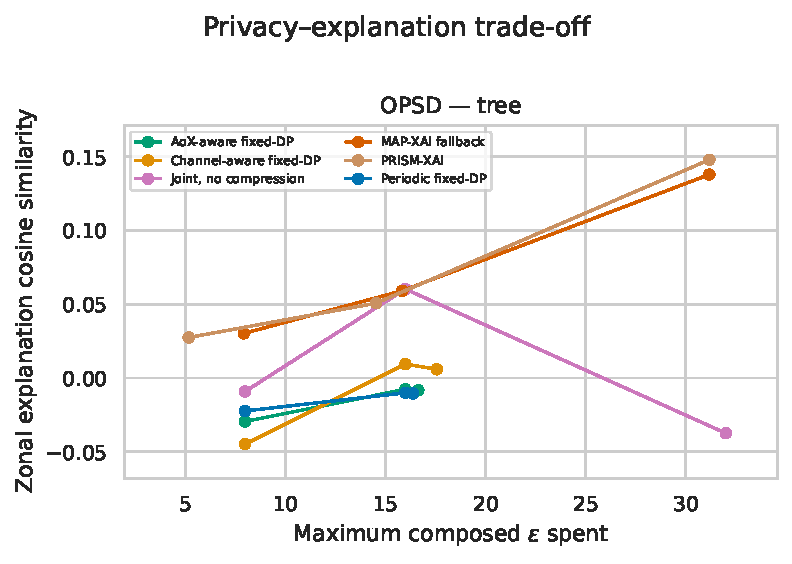
\includegraphics[width=.96\textwidth,height=.82\textheight,keepaspectratio]{../../SERVICE_TRADEOFF_RESULTS/runs/thr_3_cap_32/opsd/privacy_fidelity.pdf}

\caption{Public-score threshold $\tau=3$, release cap $M=32$, OPSD: privacy--fidelity plane. This panel should be read with the setting-level quantitative interpretation and the complete tables immediately preceding the figure block.}

\end{figure*}

\clearpage

\begin{figure*}[p]

\centering

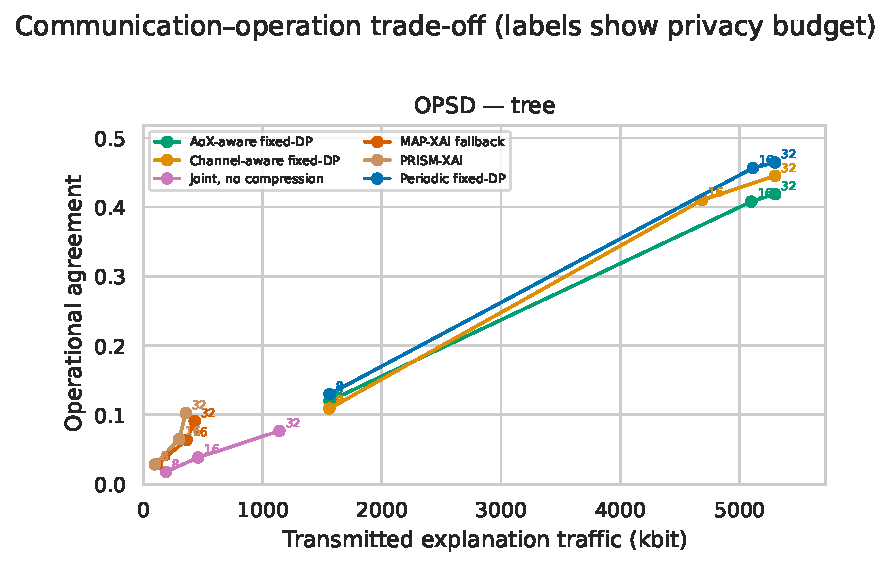
\includegraphics[width=.96\textwidth,height=.82\textheight,keepaspectratio]{../../SERVICE_TRADEOFF_RESULTS/runs/thr_3_cap_32/opsd/pareto_bits_fidelity.pdf}

\caption{Public-score threshold $\tau=3$, release cap $M=32$, OPSD: traffic--fidelity Pareto plane. This panel should be read with the setting-level quantitative interpretation and the complete tables immediately preceding the figure block.}

\end{figure*}

\clearpage

\begin{figure*}[p]

\centering

\includegraphics[width=.96\textwidth,height=.82\textheight,keepaspectratio]{../../SERVICE_TRADEOFF_RESULTS/runs/thr_3_cap_32/opsd/ablation_results.pdf}

\caption{Public-score threshold $\tau=3$, release cap $M=32$, OPSD: component ablation. This panel should be read with the setting-level quantitative interpretation and the complete tables immediately preceding the figure block.}

\end{figure*}

\clearpage

\paragraph{UCI.} The three generated tables below report the full method means, all condition-level values, and paired differences. The five figures that follow provide the corresponding temporal, fairness, privacy, Pareto, and ablation views. Aggregate panels support the setting-level summary above; dataset panels reveal whether that summary is shared by OPSD and UCI rather than being driven by their different endpoint counts.

\begin{table*}[p]\centering\tiny

\caption{Public-score threshold $\tau=3$, release cap $M=32$, UCI: complete generated method table.}

\label{tab:thr_3_cap_32:uci:main}

\resizebox{\linewidth}{!}{% Values are means with 95% Student-t confidence intervals across seeds.
\begin{tabular}{lccccccccccccccc}
\toprule
Dataset & Model & $\epsilon_{\max}$ & Method & Top-$K$ & Cosine & Decision & Recall & Prec. & Abst. & P95 ms & kbit & Spent $\epsilon$ & False int. & bit/correct & Fairness \\
\midrule
UCI & Tree & 8 & AoX-aware fixed-DP & 0.263 $\pm$ 0.041 & -0.007 $\pm$ 0.009 & 0.457 $\pm$ 0.031 & 0.457 $\pm$ 0.031 & 0.362 $\pm$ 0.024 & 0.003 $\pm$ 0.001 & 7.500 $\pm$ 0.000 & 5300.224 $\pm$ 0.000 & 7.990 $\pm$ 0.000 & 0.557 $\pm$ 0.025 & 14002.896 $\pm$ 1040.243 & 0.999 $\pm$ 0.000 \\
UCI & Tree & 8 & AoX-aware fixed-DP & 0.260 $\pm$ 0.022 & 0.010 $\pm$ 0.055 & 0.455 $\pm$ 0.047 & 0.455 $\pm$ 0.047 & 0.361 $\pm$ 0.038 & 0.003 $\pm$ 0.001 & 7.500 $\pm$ 0.000 & 5300.224 $\pm$ 0.000 & 7.990 $\pm$ 0.000 & 0.557 $\pm$ 0.048 & 14198.303 $\pm$ 1508.274 & 0.999 $\pm$ 0.000 \\
UCI & Tree & 8 & Channel-aware fixed-DP & 0.248 $\pm$ 0.031 & 0.004 $\pm$ 0.012 & 0.001 $\pm$ 0.001 & 0.001 $\pm$ 0.001 & 0.150 $\pm$ 0.151 & 0.999 $\pm$ 0.001 & 4.609 $\pm$ 1.781 & 5295.177 $\pm$ 3.740 & 7.990 $\pm$ 0.000 & 0.001 $\pm$ 0.001 & 4632196.500 $\pm$ 2102650.252 & 0.991 $\pm$ 0.001 \\
UCI & Tree & 8 & Channel-aware fixed-DP & 0.239 $\pm$ 0.030 & -0.020 $\pm$ 0.055 & 0.000 $\pm$ 0.000 & 0.000 $\pm$ 0.000 & 0.117 $\pm$ 0.225 & 0.999 $\pm$ 0.001 & 4.609 $\pm$ 1.781 & 5295.177 $\pm$ 3.740 & 7.990 $\pm$ 0.000 & 0.001 $\pm$ 0.001 & 5296989.000 $\pm$ 41104.572 & 0.991 $\pm$ 0.001 \\
UCI & Tree & 8 & Joint, no compression & 0.286 $\pm$ 0.045 & 0.004 $\pm$ 0.020 & 0.052 $\pm$ 0.005 & 0.052 $\pm$ 0.005 & 0.406 $\pm$ 0.037 & 0.875 $\pm$ 0.003 & 5.123 $\pm$ 1.792 & 672.300 $\pm$ 0.452 & 7.990 $\pm$ 0.000 & 0.053 $\pm$ 0.004 & 15676.175 $\pm$ 1475.621 & 0.994 $\pm$ 0.003 \\
UCI & Tree & 8 & Joint, no compression & 0.229 $\pm$ 0.052 & -0.032 $\pm$ 0.050 & 0.057 $\pm$ 0.007 & 0.057 $\pm$ 0.007 & 0.428 $\pm$ 0.041 & 0.875 $\pm$ 0.003 & 5.131 $\pm$ 1.787 & 672.300 $\pm$ 0.452 & 7.990 $\pm$ 0.000 & 0.052 $\pm$ 0.004 & 14702.786 $\pm$ 2334.488 & 0.994 $\pm$ 0.003 \\
UCI & Tree & 8 & Periodic fixed-DP & 0.259 $\pm$ 0.060 & -0.005 $\pm$ 0.008 & 0.006 $\pm$ 0.001 & 0.006 $\pm$ 0.001 & 0.244 $\pm$ 0.049 & 0.989 $\pm$ 0.001 & 4.596 $\pm$ 1.788 & 5299.318 $\pm$ 1.451 & 7.786 $\pm$ 0.000 & 0.013 $\pm$ 0.002 & 1215103.896 $\pm$ 390671.319 & 0.999 $\pm$ 0.000 \\
UCI & Tree & 8 & Periodic fixed-DP & 0.260 $\pm$ 0.044 & 0.022 $\pm$ 0.070 & 0.005 $\pm$ 0.001 & 0.005 $\pm$ 0.001 & 0.195 $\pm$ 0.050 & 0.989 $\pm$ 0.001 & 4.596 $\pm$ 1.788 & 5299.318 $\pm$ 1.451 & 7.786 $\pm$ 0.000 & 0.015 $\pm$ 0.002 & 1555837.203 $\pm$ 955472.503 & 0.999 $\pm$ 0.000 \\
UCI & Tree & 8 & PRISM-XAI & 0.207 $\pm$ 0.052 & 0.004 $\pm$ 0.012 & 0.046 $\pm$ 0.010 & 0.046 $\pm$ 0.010 & 0.469 $\pm$ 0.081 & 0.901 $\pm$ 0.005 & 5.035 $\pm$ 1.860 & 341.133 $\pm$ 1.293 & 6.779 $\pm$ 0.208 & 0.035 $\pm$ 0.005 & 9780.191 $\pm$ 2585.599 & 0.988 $\pm$ 0.003 \\
UCI & Tree & 8 & PRISM-XAI & 0.256 $\pm$ 0.043 & 0.000 $\pm$ 0.081 & 0.047 $\pm$ 0.008 & 0.047 $\pm$ 0.008 & 0.503 $\pm$ 0.086 & 0.902 $\pm$ 0.005 & 5.524 $\pm$ 1.825 & 338.064 $\pm$ 2.047 & 6.657 $\pm$ 0.214 & 0.032 $\pm$ 0.007 & 9159.950 $\pm$ 1670.303 & 0.989 $\pm$ 0.003 \\
UCI & Tree & 8 & MAP-XAI fallback & 0.193 $\pm$ 0.046 & 0.014 $\pm$ 0.010 & 0.046 $\pm$ 0.007 & 0.046 $\pm$ 0.007 & 0.479 $\pm$ 0.053 & 0.901 $\pm$ 0.005 & 5.106 $\pm$ 1.806 & 395.052 $\pm$ 0.314 & 7.924 $\pm$ 0.000 & 0.035 $\pm$ 0.004 & 10596.392 $\pm$ 1554.907 & 0.988 $\pm$ 0.003 \\
UCI & Tree & 8 & MAP-XAI fallback & 0.246 $\pm$ 0.061 & 0.064 $\pm$ 0.067 & 0.049 $\pm$ 0.007 & 0.049 $\pm$ 0.007 & 0.510 $\pm$ 0.076 & 0.902 $\pm$ 0.005 & 5.409 $\pm$ 1.720 & 395.226 $\pm$ 1.353 & 7.924 $\pm$ 0.000 & 0.033 $\pm$ 0.007 & 10216.728 $\pm$ 2063.280 & 0.989 $\pm$ 0.003 \\
\bottomrule
\end{tabular}
}

\end{table*}\clearpage

\begin{table*}[p]\centering\tiny

\caption{Public-score threshold $\tau=3$, release cap $M=32$, UCI: complete condition-level generated table.}

\label{tab:thr_3_cap_32:uci:conditions}

\resizebox{\textwidth}{!}{\begin{tabular}{llllccccccccccc}
\toprule
Dataset & Model & $\epsilon_{\max}$ & Method & kbit & Top-$K$ & Random Top-$K$ & Cosine & Decision & Recall & Precision & Coverage & Abstain & False int. & Spent $\epsilon$ \\
\midrule
UCI & Tree & 8 & Joint, no compression & 672.300 $\pm$ 0.452 & 0.286 $\pm$ 0.045 & 0.250 $\pm$ 0.000 & 0.004 $\pm$ 0.020 & 0.052 $\pm$ 0.005 & 0.052 $\pm$ 0.005 & 0.406 $\pm$ 0.037 & 0.125 $\pm$ 0.003 & 0.875 $\pm$ 0.003 & 0.053 $\pm$ 0.004 & 7.990 $\pm$ 0.000 \\
UCI & Tree & 8 & Joint, no compression & 672.300 $\pm$ 0.452 & 0.229 $\pm$ 0.052 & 0.250 $\pm$ 0.000 & -0.032 $\pm$ 0.050 & 0.057 $\pm$ 0.007 & 0.057 $\pm$ 0.007 & 0.428 $\pm$ 0.041 & 0.125 $\pm$ 0.003 & 0.875 $\pm$ 0.003 & 0.052 $\pm$ 0.004 & 7.990 $\pm$ 0.000 \\
UCI & Tree & 8 & Periodic fixed-DP & 5299.318 $\pm$ 1.451 & 0.259 $\pm$ 0.060 & 0.250 $\pm$ 0.000 & -0.005 $\pm$ 0.008 & 0.006 $\pm$ 0.001 & 0.006 $\pm$ 0.001 & 0.244 $\pm$ 0.049 & 0.011 $\pm$ 0.001 & 0.989 $\pm$ 0.001 & 0.013 $\pm$ 0.002 & 7.786 $\pm$ 0.000 \\
UCI & Tree & 8 & Periodic fixed-DP & 5299.318 $\pm$ 1.451 & 0.260 $\pm$ 0.044 & 0.250 $\pm$ 0.000 & 0.022 $\pm$ 0.070 & 0.005 $\pm$ 0.001 & 0.005 $\pm$ 0.001 & 0.195 $\pm$ 0.050 & 0.011 $\pm$ 0.001 & 0.989 $\pm$ 0.001 & 0.015 $\pm$ 0.002 & 7.786 $\pm$ 0.000 \\
UCI & Tree & 8 & PRISM-XAI & 341.133 $\pm$ 1.293 & 0.207 $\pm$ 0.052 & 0.250 $\pm$ 0.000 & 0.004 $\pm$ 0.012 & 0.046 $\pm$ 0.010 & 0.046 $\pm$ 0.010 & 0.469 $\pm$ 0.081 & 0.099 $\pm$ 0.005 & 0.901 $\pm$ 0.005 & 0.035 $\pm$ 0.005 & 6.779 $\pm$ 0.208 \\
UCI & Tree & 8 & PRISM-XAI & 338.064 $\pm$ 2.047 & 0.256 $\pm$ 0.043 & 0.250 $\pm$ 0.000 & 0.000 $\pm$ 0.081 & 0.047 $\pm$ 0.008 & 0.047 $\pm$ 0.008 & 0.503 $\pm$ 0.086 & 0.098 $\pm$ 0.005 & 0.902 $\pm$ 0.005 & 0.032 $\pm$ 0.007 & 6.657 $\pm$ 0.214 \\
UCI & Tree & 16 & Joint, no compression & 1632.150 $\pm$ 0.339 & 0.216 $\pm$ 0.041 & 0.250 $\pm$ 0.000 & 0.001 $\pm$ 0.012 & 0.094 $\pm$ 0.005 & 0.094 $\pm$ 0.005 & 0.330 $\pm$ 0.024 & 0.228 $\pm$ 0.005 & 0.772 $\pm$ 0.005 & 0.133 $\pm$ 0.010 & 15.997 $\pm$ 0.000 \\
UCI & Tree & 16 & Joint, no compression & 1632.600 $\pm$ 0.554 & 0.204 $\pm$ 0.011 & 0.250 $\pm$ 0.000 & -0.021 $\pm$ 0.033 & 0.099 $\pm$ 0.016 & 0.099 $\pm$ 0.016 & 0.347 $\pm$ 0.054 & 0.228 $\pm$ 0.005 & 0.772 $\pm$ 0.005 & 0.128 $\pm$ 0.011 & 15.997 $\pm$ 0.000 \\
UCI & Tree & 16 & Periodic fixed-DP & 5299.318 $\pm$ 1.451 & 0.259 $\pm$ 0.060 & 0.250 $\pm$ 0.000 & -0.005 $\pm$ 0.008 & 0.006 $\pm$ 0.001 & 0.006 $\pm$ 0.001 & 0.244 $\pm$ 0.049 & 0.011 $\pm$ 0.001 & 0.989 $\pm$ 0.001 & 0.013 $\pm$ 0.002 & 7.786 $\pm$ 0.000 \\
UCI & Tree & 16 & Periodic fixed-DP & 5299.318 $\pm$ 1.451 & 0.260 $\pm$ 0.044 & 0.250 $\pm$ 0.000 & 0.022 $\pm$ 0.070 & 0.005 $\pm$ 0.001 & 0.005 $\pm$ 0.001 & 0.195 $\pm$ 0.050 & 0.011 $\pm$ 0.001 & 0.989 $\pm$ 0.001 & 0.015 $\pm$ 0.002 & 7.786 $\pm$ 0.000 \\
UCI & Tree & 16 & PRISM-XAI & 1110.802 $\pm$ 3.293 & 0.269 $\pm$ 0.046 & 0.250 $\pm$ 0.000 & 0.018 $\pm$ 0.010 & 0.126 $\pm$ 0.013 & 0.126 $\pm$ 0.013 & 0.407 $\pm$ 0.047 & 0.285 $\pm$ 0.006 & 0.715 $\pm$ 0.006 & 0.127 $\pm$ 0.012 & 15.063 $\pm$ 0.065 \\
UCI & Tree & 16 & PRISM-XAI & 1099.581 $\pm$ 2.815 & 0.240 $\pm$ 0.048 & 0.250 $\pm$ 0.000 & -0.063 $\pm$ 0.054 & 0.115 $\pm$ 0.016 & 0.115 $\pm$ 0.016 & 0.379 $\pm$ 0.064 & 0.282 $\pm$ 0.007 & 0.718 $\pm$ 0.007 & 0.132 $\pm$ 0.019 & 14.998 $\pm$ 0.062 \\
UCI & Tree & 32 & Joint, no compression & 4034.550 $\pm$ 5.034 & 0.246 $\pm$ 0.031 & 0.250 $\pm$ 0.000 & -0.002 $\pm$ 0.015 & 0.228 $\pm$ 0.013 & 0.228 $\pm$ 0.013 & 0.361 $\pm$ 0.028 & 0.537 $\pm$ 0.009 & 0.463 $\pm$ 0.009 & 0.279 $\pm$ 0.017 & 31.999 $\pm$ 0.000 \\
UCI & Tree & 32 & Joint, no compression & 4034.550 $\pm$ 5.034 & 0.241 $\pm$ 0.033 & 0.250 $\pm$ 0.000 & -0.012 $\pm$ 0.030 & 0.228 $\pm$ 0.028 & 0.228 $\pm$ 0.028 & 0.360 $\pm$ 0.047 & 0.530 $\pm$ 0.010 & 0.470 $\pm$ 0.010 & 0.280 $\pm$ 0.026 & 31.999 $\pm$ 0.000 \\
UCI & Tree & 32 & Periodic fixed-DP & 5299.318 $\pm$ 1.451 & 0.259 $\pm$ 0.060 & 0.250 $\pm$ 0.000 & -0.005 $\pm$ 0.008 & 0.006 $\pm$ 0.001 & 0.006 $\pm$ 0.001 & 0.244 $\pm$ 0.049 & 0.011 $\pm$ 0.001 & 0.989 $\pm$ 0.001 & 0.013 $\pm$ 0.002 & 7.786 $\pm$ 0.000 \\
UCI & Tree & 32 & Periodic fixed-DP & 5299.318 $\pm$ 1.451 & 0.260 $\pm$ 0.044 & 0.250 $\pm$ 0.000 & 0.022 $\pm$ 0.070 & 0.005 $\pm$ 0.001 & 0.005 $\pm$ 0.001 & 0.195 $\pm$ 0.050 & 0.011 $\pm$ 0.001 & 0.989 $\pm$ 0.001 & 0.015 $\pm$ 0.002 & 7.786 $\pm$ 0.000 \\
UCI & Tree & 32 & PRISM-XAI & 1317.135 $\pm$ 2.878 & 0.286 $\pm$ 0.041 & 0.250 $\pm$ 0.000 & 0.016 $\pm$ 0.014 & 0.150 $\pm$ 0.019 & 0.150 $\pm$ 0.019 & 0.423 $\pm$ 0.062 & 0.338 $\pm$ 0.007 & 0.662 $\pm$ 0.007 & 0.143 $\pm$ 0.016 & 31.175 $\pm$ 0.000 \\
UCI & Tree & 32 & PRISM-XAI & 1302.454 $\pm$ 3.178 & 0.249 $\pm$ 0.044 & 0.250 $\pm$ 0.000 & -0.087 $\pm$ 0.048 & 0.148 $\pm$ 0.011 & 0.148 $\pm$ 0.011 & 0.437 $\pm$ 0.045 & 0.335 $\pm$ 0.007 & 0.665 $\pm$ 0.007 & 0.132 $\pm$ 0.013 & 31.175 $\pm$ 0.000 \\
\bottomrule
\end{tabular}
}

\end{table*}\clearpage

\begin{table*}[p]\centering\tiny

\caption{Public-score threshold $\tau=3$, release cap $M=32$, UCI: complete generated paired comparisons.}

\label{tab:thr_3_cap_32:uci:paired}

\resizebox{\textwidth}{!}{\begin{tabular}{llcccc}
\toprule
Dataset & Baseline & Delta kbit & Delta Top-$K$ & Delta recall & Delta fairness \\
\midrule
UCI & AoX-aware fixed-DP & -4959.091 $\pm$ 1.293 & -0.056 $\pm$ 0.063 & -0.411 $\pm$ 0.026 & -0.011 $\pm$ 0.003 \\
UCI & AoX-aware fixed-DP & -4189.422 $\pm$ 3.293 & 0.005 $\pm$ 0.058 & -0.332 $\pm$ 0.035 & -0.002 $\pm$ 0.001 \\
UCI & AoX-aware fixed-DP & -3983.089 $\pm$ 2.878 & 0.023 $\pm$ 0.064 & -0.307 $\pm$ 0.043 & -0.001 $\pm$ 0.001 \\
UCI & AoX-aware fixed-DP & -4962.160 $\pm$ 2.047 & -0.004 $\pm$ 0.042 & -0.409 $\pm$ 0.046 & -0.010 $\pm$ 0.003 \\
UCI & AoX-aware fixed-DP & -4200.643 $\pm$ 2.815 & -0.020 $\pm$ 0.050 & -0.340 $\pm$ 0.048 & -0.002 $\pm$ 0.001 \\
UCI & AoX-aware fixed-DP & -3997.770 $\pm$ 3.178 & -0.012 $\pm$ 0.032 & -0.307 $\pm$ 0.052 & -0.001 $\pm$ 0.001 \\
UCI & Channel-aware fixed-DP & -4954.044 $\pm$ 4.047 & -0.041 $\pm$ 0.066 & 0.046 $\pm$ 0.010 & -0.002 $\pm$ 0.003 \\
UCI & Channel-aware fixed-DP & -4189.422 $\pm$ 3.293 & 0.001 $\pm$ 0.058 & 0.125 $\pm$ 0.013 & 0.667 $\pm$ 0.001 \\
UCI & Channel-aware fixed-DP & -3983.089 $\pm$ 2.878 & 0.018 $\pm$ 0.049 & 0.150 $\pm$ 0.019 & 0.743 $\pm$ 0.001 \\
UCI & Channel-aware fixed-DP & -4957.113 $\pm$ 4.745 & 0.017 $\pm$ 0.045 & 0.046 $\pm$ 0.008 & -0.002 $\pm$ 0.003 \\
UCI & Channel-aware fixed-DP & -4200.643 $\pm$ 2.815 & -0.020 $\pm$ 0.052 & 0.115 $\pm$ 0.016 & 0.667 $\pm$ 0.001 \\
UCI & Channel-aware fixed-DP & -3997.770 $\pm$ 3.178 & -0.011 $\pm$ 0.043 & 0.148 $\pm$ 0.011 & 0.743 $\pm$ 0.001 \\
UCI & Joint, no compression & -331.167 $\pm$ 1.523 & -0.079 $\pm$ 0.085 & -0.006 $\pm$ 0.011 & -0.006 $\pm$ 0.003 \\
UCI & Joint, no compression & -521.348 $\pm$ 3.369 & 0.052 $\pm$ 0.038 & 0.031 $\pm$ 0.015 & -0.000 $\pm$ 0.001 \\
UCI & Joint, no compression & -2717.415 $\pm$ 6.000 & 0.040 $\pm$ 0.049 & -0.077 $\pm$ 0.014 & -0.001 $\pm$ 0.001 \\
UCI & Joint, no compression & -334.236 $\pm$ 2.296 & 0.026 $\pm$ 0.066 & -0.010 $\pm$ 0.011 & -0.005 $\pm$ 0.003 \\
UCI & Joint, no compression & -533.019 $\pm$ 2.619 & 0.037 $\pm$ 0.048 & 0.016 $\pm$ 0.022 & -0.000 $\pm$ 0.001 \\
UCI & Joint, no compression & -2732.096 $\pm$ 5.519 & 0.007 $\pm$ 0.058 & -0.080 $\pm$ 0.032 & -0.001 $\pm$ 0.001 \\
UCI & Periodic fixed-DP & -4958.185 $\pm$ 2.040 & -0.053 $\pm$ 0.077 & 0.040 $\pm$ 0.010 & -0.011 $\pm$ 0.003 \\
UCI & Periodic fixed-DP & -4188.516 $\pm$ 3.590 & 0.009 $\pm$ 0.089 & 0.120 $\pm$ 0.014 & -0.002 $\pm$ 0.001 \\
UCI & Periodic fixed-DP & -3982.184 $\pm$ 3.108 & 0.027 $\pm$ 0.068 & 0.145 $\pm$ 0.020 & -0.002 $\pm$ 0.001 \\
UCI & Periodic fixed-DP & -4961.254 $\pm$ 2.973 & -0.005 $\pm$ 0.068 & 0.041 $\pm$ 0.007 & -0.011 $\pm$ 0.003 \\
UCI & Periodic fixed-DP & -4199.738 $\pm$ 3.048 & -0.020 $\pm$ 0.078 & 0.109 $\pm$ 0.015 & -0.002 $\pm$ 0.001 \\
UCI & Periodic fixed-DP & -3996.864 $\pm$ 3.261 & -0.012 $\pm$ 0.073 & 0.142 $\pm$ 0.011 & -0.002 $\pm$ 0.001 \\
UCI & MAP-XAI fallback & -53.919 $\pm$ 1.196 & 0.014 $\pm$ 0.036 & -0.000 $\pm$ 0.005 & 0.000 $\pm$ 0.000 \\
UCI & MAP-XAI fallback & -182.879 $\pm$ 3.287 & 0.006 $\pm$ 0.059 & -0.002 $\pm$ 0.010 & 0.000 $\pm$ 0.000 \\
UCI & MAP-XAI fallback & -216.465 $\pm$ 2.875 & 0.076 $\pm$ 0.044 & 0.002 $\pm$ 0.015 & 0.000 $\pm$ 0.000 \\
UCI & MAP-XAI fallback & -57.162 $\pm$ 1.160 & 0.010 $\pm$ 0.051 & -0.002 $\pm$ 0.008 & -0.000 $\pm$ 0.001 \\
UCI & MAP-XAI fallback & -193.593 $\pm$ 2.996 & 0.006 $\pm$ 0.034 & -0.010 $\pm$ 0.011 & -0.000 $\pm$ 0.000 \\
UCI & MAP-XAI fallback & -230.577 $\pm$ 3.247 & 0.018 $\pm$ 0.059 & 0.003 $\pm$ 0.011 & -0.000 $\pm$ 0.000 \\
\bottomrule
\end{tabular}
}

\end{table*}\clearpage

\begin{figure*}[p]

\centering

\includegraphics[width=.96\textwidth,height=.82\textheight,keepaspectratio]{../../SERVICE_TRADEOFF_RESULTS/runs/thr_3_cap_32/uci/regime_trace.pdf}

\caption{Public-score threshold $\tau=3$, release cap $M=32$, UCI: representative regime trace. This panel should be read with the setting-level quantitative interpretation and the complete tables immediately preceding the figure block.}

\end{figure*}

\clearpage

\begin{figure*}[p]

\centering

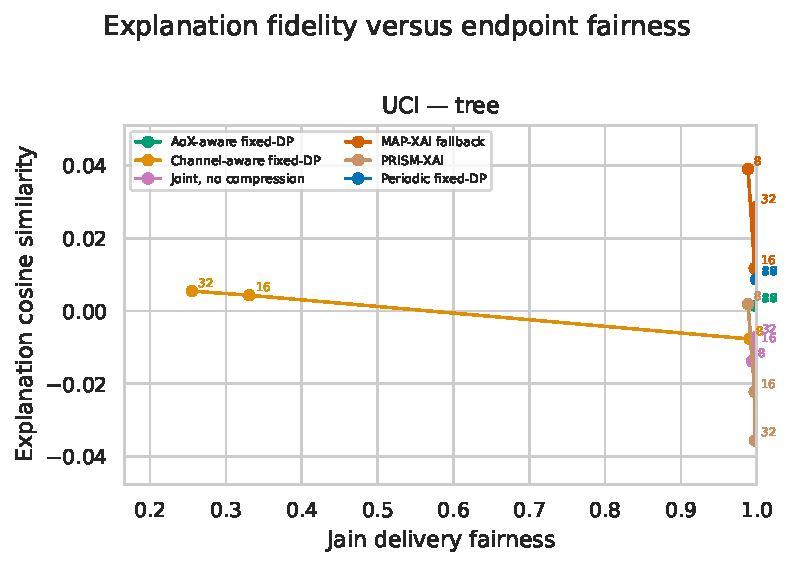
\includegraphics[width=.96\textwidth,height=.82\textheight,keepaspectratio]{../../SERVICE_TRADEOFF_RESULTS/runs/thr_3_cap_32/uci/fairness_reliability.pdf}

\caption{Public-score threshold $\tau=3$, release cap $M=32$, UCI: fairness--reliability plane. This panel should be read with the setting-level quantitative interpretation and the complete tables immediately preceding the figure block.}

\end{figure*}

\clearpage

\begin{figure*}[p]

\centering

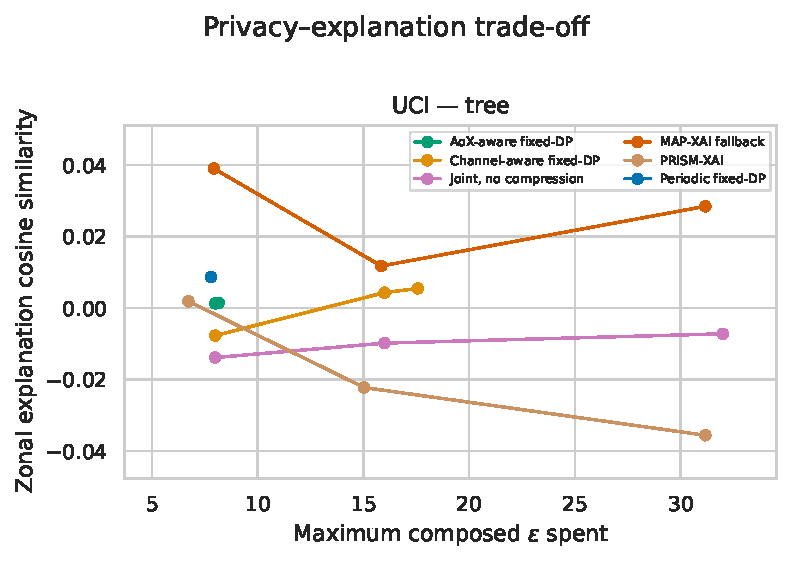
\includegraphics[width=.96\textwidth,height=.82\textheight,keepaspectratio]{../../SERVICE_TRADEOFF_RESULTS/runs/thr_3_cap_32/uci/privacy_fidelity.pdf}

\caption{Public-score threshold $\tau=3$, release cap $M=32$, UCI: privacy--fidelity plane. This panel should be read with the setting-level quantitative interpretation and the complete tables immediately preceding the figure block.}

\end{figure*}

\clearpage

\begin{figure*}[p]

\centering

\includegraphics[width=.96\textwidth,height=.82\textheight,keepaspectratio]{../../SERVICE_TRADEOFF_RESULTS/runs/thr_3_cap_32/uci/pareto_bits_fidelity.pdf}

\caption{Public-score threshold $\tau=3$, release cap $M=32$, UCI: traffic--fidelity Pareto plane. This panel should be read with the setting-level quantitative interpretation and the complete tables immediately preceding the figure block.}

\end{figure*}

\clearpage

\begin{figure*}[p]

\centering

\includegraphics[width=.96\textwidth,height=.82\textheight,keepaspectratio]{../../SERVICE_TRADEOFF_RESULTS/runs/thr_3_cap_32/uci/ablation_results.pdf}

\caption{Public-score threshold $\tau=3$, release cap $M=32$, UCI: component ablation. This panel should be read with the setting-level quantitative interpretation and the complete tables immediately preceding the figure block.}

\end{figure*}

\clearpage

\FloatBarrier

\subsection{What the complete sweep establishes}

The threshold and release cap have different roles. At fixed $M=8$, raising $\tau$ primarily moves coverage and recall while traffic remains near 205--209~kbit. Raising $M$ changes the available service region more strongly and increases traffic. PRISM-XAI remains below MAP-XAI-only traffic throughout the observed grid, with aggregate-mean ratio savings between 14.35\% and 16.56\%. The complete matched-region condition, however, is preserved across all cells only at $M=8$; conclusions at larger caps are therefore descriptive trade-off results. The fidelity and fairness panels add diagnostic context but do not convert the service proxies into evidence of operational grid benefit. Together, the sweep supports a configurable communication scheduler whose operating point must be chosen from an explicit traffic--service requirement rather than from traffic alone.
